\PassOptionsToPackage{unicode=true}{hyperref} % options for packages loaded elsewhere
\PassOptionsToPackage{hyphens}{url}
\PassOptionsToPackage{shortlabels}{enumitem}
\documentclass[b5paper,11pt,twoside,openright]{book}

\usepackage{ifxetex}
\ifxetex{}
\else
\errmessage{Must be built with XeLaTeX}
\fi

\usepackage{amsmath}
\usepackage{fontspec}
\usepackage{fourier-otf} % erewhon-math
\setmonofont{iosevka-type-slab-regular}[
  Path=../common/iosevka-type-slab/,
  Extension=.ttf,
  BoldFont=iosevka-type-slab-bold,
  ItalicFont=iosevka-type-slab-italic,
  BoldItalicFont=iosevka-type-slab-bolditalic,
  Scale=MatchLowercase,
]

% Math
\usepackage[binary-units]{siunitx}

\usepackage{caption}
\usepackage{authblk}
\usepackage{enumitem}
\usepackage{footnote}

% Table
\usepackage{tabu}
\usepackage{longtable}
\usepackage{booktabs}
\usepackage{multirow}

% Verbatim & Source code
\usepackage{fancyvrb}
\usepackage{minted}

% Beauty
\usepackage[protrusion]{microtype}
\usepackage[defaultlines=3]{nowidow}
\usepackage{upquote}
\usepackage{parskip}
\usepackage[strict]{changepage}

\usepackage{hyperref}

% Graph
\usepackage{graphicx}
\usepackage{grffile}
\usepackage{tikz}

\usepackage{alltt}
\usepackage{enumitem}
\usepackage{fixltx2e}
\usepackage{multicol}
\usepackage{pdfpages} % include cover page
\usepackage{ragged2e}
\usepackage{rotating}
\usepackage{tocstyle}
\hypersetup{
  bookmarksnumbered,
  pdfborder={0 0 0},
  pdfpagemode=UseNone,
  pdfstartview=FitH,
  breaklinks=true}
\urlstyle{same}  % don't use monospace font for urls

\usetikzlibrary{arrows.meta,calc,shapes.geometric,shapes.misc}

\setminted{
  autogobble,
  breakbytokenanywhere,
  breaklines,
  fontsize=\footnotesize,
}
\setmintedinline{
  autogobble,
  breakbytokenanywhere,
  breaklines,
  fontsize=\footnotesize,
}

\makeatletter
\def\maxwidth{\ifdim\Gin@nat@width>\linewidth\linewidth\else\Gin@nat@width\fi}
\def\maxheight{\ifdim\Gin@nat@height>\textheight\textheight\else\Gin@nat@height\fi}
\makeatother

% Scale images if necessary, so that they will not overflow the page
% margins by default, and it is still possible to overwrite the defaults
% using explicit options in \includegraphics[width, height, ...]{}
\setkeys{Gin}{width=\maxwidth,height=\maxheight,keepaspectratio}
\setlength{\emergencystretch}{3em}  % prevent overfull lines
\setcounter{secnumdepth}{3}

% Redefines (sub)paragraphs to behave more like sections
\ifx\paragraph\undefined\else
\let\oldparagraph\paragraph{}
\renewcommand{\paragraph}[1]{\oldparagraph{#1}\mbox{}}
\fi
\ifx\subparagraph\undefined\else
\let\oldsubparagraph\subparagraph{}
\renewcommand{\subparagraph}[1]{\oldsubparagraph{#1}\mbox{}}
\fi

% set default figure placement to htbp
\makeatletter
\def\fps@figure{htbp}
\makeatother

\setlist{noitemsep}
\usetocstyle{standard}

\usetikzlibrary{calc,shapes.multipart,chains,arrows,matrix}
\tikzset{>=latex'}
\tikzstyle{list}=[
	 rectangle split,
	 rectangle split parts=2, draw,
	 rectangle split horizontal,
	 rectangle split part align=base,
	 text width=3ex, text centered
    ]

\newcommand{\pFF}[2]{\draw[->] let \p1 = (#1.one), \p2 = (#1.center), \p3 = (#2.one), \p4 = (#2.north) in (\x1,\y2) -- (\x3,\y4)}
\newcommand{\pSF}[2]{\draw[->] let \p1 = (#1.two), \p2 = (#1.center), \p3 = (#2.west), \p4 = (#2.center) in (\x1,\y2) -- (\x3,\y4)}

\newcolumntype{L}{>{\RaggedRight}X}

\newcommand{\SpecialChapter}[1]{%
  \chapter*{#1}%
  \addcontentsline{toc}{chapter}{#1}%
  \markboth{\MakeUppercase{#1}}{\MakeUppercase{#1}}
}

\begin{document}

\pagestyle{empty}

\pdfbookmark[0]{Cover}{cover}
\includepdf[fitpaper]{canned/cover-A4}

\cleardoublepage{}

\pagestyle{headings}

\setcounter{page}{1}
\pagenumbering{roman}
\pdfbookmark{\contentsname}{toc}
\tableofcontents

\SpecialChapter{Preface}

\label{preface_h0}




Scheme was introduced in 1975 by Gerald J. Sussman
and
Guy L. Steele Jr. [\hyperref[bibliography_g246]{28},\hyperref[bibliography_g247]{29}],
and was the
first dialect of \label{preface_s0}Lisp to fully support lexical scoping, first-class
procedures, and continuations.
In its earliest form it was a small language intended primarily
for research and teaching, supporting only a handful of predefined
syntactic forms and procedures.
Scheme is now a complete general-purpose programming language,
though it still derives its power from a small set of key concepts.
Early implementations of the language were interpreter-based
and slow, but some current Scheme implementations boast sophisticated
compilers that generate code on par with code generated by the best
optimizing compilers for lower-level languages such as C and Fortran.


This book is intended to provide an introduction to the Scheme programming language
but not an introduction to programming in general.
The reader is expected to have had some experience programming and
to be familiar with terms commonly associated with computers and
programming languages.
Readers unfamiliar with Scheme or Lisp should
also consider reading \textit{The Little Schemer} [\hyperref[bibliography_g231]{13}] to become familiar with
the concepts of list processing and recursion.
Readers new to programming should begin with an introductory text on
programming.


Scheme has been standardized both formally and informally.
The \label{preface_s1}\textit{IEEE Standard for the Scheme Programming
Language} [\hyperref[bibliography_g236]{18}], describes a formal
ANSI/IEEE Standard for Scheme but dates back to 1991.
A related series of reports, the "\label{preface_s2}Revised Reports on the
Algorithmic Language Scheme," document an evolving informal standard that
most implementations support.
The current report in this series is the "Revised\textsuperscript{6} Report on the
Algorithmic Language Scheme" [\hyperref[bibliography_g242]{24}], which was completed in 2007.


This book covers the language of the Revised\textsuperscript{6} Report.
It is not intended to supplant the Revised\textsuperscript{6} Report but rather to
provide a more comprehensive introduction and reference
manual for the language, with more explanatory text and examples,
suitable more for users than for implementors.
Features specific to particular implementations of Scheme are not included.
In particular, features specific to the author's
\label{preface_s3}Chez Scheme and
\label{preface_s4}Petite Chez Scheme implementations are described separately
in the \textit{Chez Scheme User's Guide} [\hyperref[bibliography_g227]{9}].
On the other hand, no book on Scheme would be complete without some coverage
of the interactive top level, since nearly every Scheme system supports interactive
use in one form or another, even though the behavior is not standardized by the
Revised\textsuperscript{6} Report.
Chapters 2 and 3 are thus written assuming that the reader has available a Scheme
implementation that supports an interactive top level, with behavior consistent
with the description of the top-level environment in earlier reports and the
IEEE/ANSI standard.


A large number of small- to medium-sized examples are spread throughout
the text, and one entire chapter is dedicated to the presentation of a
set of longer examples.
Many of the examples show how a standard Scheme syntactic form or
procedure might be implemented;
others implement useful extensions.
All of the examples can
be entered directly from the keyboard into an interactive Scheme
session.


This book is organized into twelve chapters, plus back matter.
Chapter \ref{intro_g0} describes the properties and features of
Scheme that make it a useful and enjoyable language to use.
Chapter \ref{intro_g0} also describes Scheme's notational conventions and the
typographical conventions employed in this book.


Chapter \ref{start_g4} is an introduction to Scheme programming
for the novice Scheme
programmer that leads the reader through a series of examples, beginning with
simple Scheme expressions and working toward progressively more
difficult ones.
Each section of Chapter \ref{start_g4} introduces
a small set of related features, and
the end of each section contains a set of exercises for further practice.
The reader will learn the most from Chapter \ref{start_g4} by
sitting at the keyboard
and typing in the examples and trying the exercises.


Chapter \ref{further_g49} continues the introduction but covers
more advanced features and concepts.
Even readers with prior Scheme experience may wish to work
through the examples and exercises found there.


Chapters \ref{binding_g88} through \hyperref[exceptions_g147]{11} make up the reference
portion of the text.
They present each of Scheme's primitive procedures and syntactic
forms in turn, grouping them into short sections of related procedures
and forms.
Chapter \ref{binding_g88} describes operations for creating procedures
and variable bindings;
Chapter \ref{control_g96}, program control operations;
Chapter \ref{objects_g106}, operations on the various object types
(including lists, numbers, and strings);
Chapter \ref{io_g121}, input and output operations;
Chapter \ref{syntax_g133}, syntactic extension;
Chapter \ref{records_g138}, record-type definitions;
Chapter \ref{libraries_g142}, libraries and top-level programs; and
Chapter \ref{exceptions_g147}, exceptions and conditions.


Chapter \ref{examples_g151} contains a collection of example procedures,
libraries, and programs, each with a short overview, some examples of
its use, the implementation with brief explanation, and a set of
exercises for further work.
Each of these programs demonstrates a particular set of features,
and together they illustrate an appropriate style for
programming in Scheme.


Following Chapter \ref{examples_g151} are
bibliographical references,
answers to selected exercises,
a detailed description of the formal syntax of Scheme programs and data,
a concise summary of Scheme syntactic forms and procedures,
and
the index.
The summary of forms and procedures is a useful first stop for
programmers unsure of the structure of a syntactic form or the
arguments expected by a primitive procedure.
The page numbers appearing in the summary of forms and procedures and
the italicized page numbers appearing in the index indicate the
locations in the text where forms and procedures are defined.


Because the reference portion describes a number of aspects of the
language not covered by the introductory chapters along with a number
of interesting short examples,
most readers will find it profitable to read through most of the
material to become familiar with each feature and how it relates to
other features.
Chapter \ref{objects_g106} is lengthy, however, and may be skimmed
and later referenced as needed.


An online version of this book is available at \href{http://www.scheme.com/tspl/}{\textit{http://www.scheme.com/tspl/}}.
The summary of forms and index in the online edition include page
numbers for the printed version and are thus useful as searchable
indexes.


\textit{About the illustrations:}
The cover illustration and the illustration at the front of each chapter
are algorithmic line fields created by artist Jean-Pierre Hébert, based
on an idea inspired by the writings of John Cage.
Each line field is created by the composition of any number of grids of
parallel lines.
The grids are regular, but they are not.
For instance, the lines are of irregular length, which creates ragged
edges.
Their tone and thickness vary slightly.
They are not exactly equidistant.
They intersect with each other at a certain angle. 
When this angle is small, patterns of interference develop.
The lines are first steeped into various scalar fields that perturb their
original straight shape, then projected on the plane of the paper.
Masks introduce holes in some layers. 
For the cover illustration, the grids are colored in different hues.


All the images are created by a single Scheme program that makes most of
the decisions, based heavily on chance.
The artist controls only canvas size, aspect ratio, the overall palette of
colors, and levels of chance and fuzziness. 
The task of the artist is to introduce just enough chance at the right
place so that the results are at the same time surprising, interesting,
and in line with the artist's sense of aesthetics. 
This is a game of uncertainty, chaos, and harmony.


\textit{Acknowledgments:}
Many individuals contributed in one way
or another to the preparation of one or more editions
of this book, including
Bruce Smith,
Eugene Kohlbecker,
Matthias Felleisen,
Dan Friedman,
Bruce Duba,
Phil Dybvig,
Guy Steele,
Bob Hieb,
Chris Haynes,
Dave Plaisted,
Joan Curry,
Frank Silbermann,
Pavel Curtis,
John Wait,
Carl Bruggeman,
Sam Daniel,
Oscar Waddell,
Mike Ashley,
John LaLonde,
John Zuckerman,
John Simmons,
Bob Prior,
Bob Burger,
and
Aziz Ghuloum.
Many others have offered minor corrections and suggestions.
Oscar Waddell helped create the typesetting system used to
format the printed and online versions of this book.
A small amount of text and a few examples have been adapted from
the Revised\textsuperscript{6} Report for this book, for which credit goes to the
editors of that report and many others who contributed to it.
Finally and most importantly, my wife, Susan Dybvig, suggested that
I write this book in the first place and lent her expertise and
assistance to the production and publication of this and the
previous editions.




\setcounter{page}{1}
\pagenumbering{arabic}
\chapter{Introduction\label{intro_CHPTINTRO}}
\label{intro_g0}
\label{intro_h0}
\begin{figure}[H]
\centering
\setlength{\fboxrule}{3pt}
\fbox{
\includegraphics[width=0.9\textwidth]{canned/ch1.png}
\begin{rotate}{90}
\copyright~2009 Jean-Pierre H\'{e}bert
\end{rotate}}
\end{figure}
\clearpage





Scheme is a general-purpose computer programming language.
It is a high-level language, supporting operations on structured
data such as strings, lists, and vectors, as well as operations on
more traditional data such as numbers and characters.
While Scheme is often identified with symbolic
applications, its rich set of data types and flexible
control structures make it a truly versatile language.
Scheme has been employed to write text editors, optimizing
compilers, operating systems, graphics packages, expert systems,
numerical applications, financial analysis packages,
virtual reality systems,
and practically every other type of application imaginable.
Scheme is a fairly simple language to learn, since it is based
on a handful of syntactic forms and semantic concepts and
since the interactive nature of most implementations encourages
experimentation.
Scheme is a challenging language to understand fully, however;
developing the ability to use its full potential requires careful study
and practice.


Scheme programs are highly portable across versions of
the same Scheme implementation on different machines, because machine
dependencies are almost completely hidden from the programmer.
They are also portable across different implementations because of the
efforts of a group of Scheme language designers who have published
a series of reports,
the "\label{intro_s0}Revised Reports" on Scheme.
The most recent, the 
"Revised\textsuperscript{6} Report" [\hyperref[bibliography_g242]{24}], emphasizes portability
through a set of standard libraries and a standard mechanism for
defining new portable libraries and top-level programs.


Although some early Scheme systems were inefficient and slow,
many newer compiler-based implementations are fast, with programs
running on par with equivalent programs written in
lower-level languages.
The relative inefficiency that sometimes remains results from run-time
checks that support generic arithmetic and help programmers
detect and correct various common
programming errors.
These checks may be disabled in many implementations.


Scheme supports many types of data values, or
\label{intro_s1}\textit{objects}, including characters, strings, symbols,
lists or vectors of objects, and a full set of numeric data types,
including complex, real, and arbitrary-precision rational numbers.


The storage required to hold the contents of an object is
\label{intro_s2}dynamically allocated as
necessary and retained until no longer needed, then automatically
deallocated, typically by a
\label{intro_s3}\textit{garbage collector} that
periodically recovers the storage used by inaccessible objects.
Simple atomic values, such as small integers, characters, booleans,
and the empty list, are typically represented as immediate values and
thus incur no allocation or deallocation overhead.


Regardless of representation,
all objects are \label{intro_s4}\textit{first-class} data values;
because they are retained indefinitely, they may be passed freely
as arguments to procedures, returned as values from procedures, and
combined to form new objects.
This is in contrast with many other languages where composite data
values such as arrays are either statically allocated and never
deallocated, allocated on entry to a block of code and unconditionally
deallocated on exit from the block, or explicitly allocated \textit{and}
deallocated by the programmer.


Scheme is a call-by-value language, but for at least mutable objects (objects
that can be modified), the values are \label{intro_s5}pointers
to the actual storage.
These pointers remain behind the scenes, however, and programmers need
not be conscious of them except to understand that the storage for an
object is not copied when an object is passed to or returned from
a procedure.


\label{intro_s6}At the heart of the Scheme language is a
small core of syntactic forms from which all other forms are built.
These core forms, a set of extended syntactic forms derived from
them, and a set of \label{intro_s7}primitive procedures
make up the full Scheme language.
An \label{intro_s8}interpreter or \label{intro_s9}compiler for Scheme
can be quite small and potentially fast and highly reliable.
The extended syntactic forms and many primitive procedures can be
defined in Scheme itself, simplifying the implementation and
increasing reliability.


Scheme programs share a common printed representation with Scheme
data structures.
As a result, any Scheme program has a natural and obvious internal
representation as a Scheme object.
For example, \label{intro_s10}variables and syntactic \label{intro_s11}keywords correspond to
symbols, while structured syntactic forms correspond to lists.
This representation is the basis for the syntactic extension
facilities
provided by Scheme for the definition of new syntactic
forms in terms of existing syntactic forms and procedures.
It also facilitates the implementation of interpreters, compilers, and
other program transformation tools for Scheme directly in Scheme, as
well as program transformation tools for other languages in Scheme.


Scheme variables and keywords are
\label{intro_s12}\textit{lexically scoped}, and
Scheme programs are
\label{intro_s13}\textit{block-structured}.
Identifiers may be imported into a program or library or bound locally
within a given block of code such as a library, program, or procedure
body.
A local \label{intro_s14}binding is visible only lexically, i.e., within the program text
that makes up the particular block of code.
An occurrence of an identifier of the same name outside this block
refers to a different binding; if no binding for the identifier
exists outside
the block, then the reference is invalid.
Blocks may be nested, and a binding in
one block may \label{intro_s15}\textit{shadow} a binding for an identifier
of the same name in a surrounding block.
The \textit{scope} of a binding is the block in which the bound identifier
is visible
minus any portions of the block in which the identifier is
shadowed.
Block structure and lexical scoping help create
programs that are
modular, easy to read, easy to maintain, and reliable.
Efficient code for lexical scoping is possible because a compiler
can determine before program evaluation the scope of all bindings
and the binding to which each identifier reference resolves.
This does not mean, of course, that a compiler can determine the
values of all variables, since the actual values are not computed
in most cases until the program executes.


In most languages, a \label{intro_s16}procedure definition is simply the association
of a name with a block of code.
Certain variables local to the block are the parameters of the
procedure.
In some languages, a procedure definition may appear within another
block or procedure so long as the procedure is invoked only during
execution of the enclosing block.
In others, procedures can be defined only at top level.
In Scheme, a procedure definition may appear within another block or
procedure, and the procedure may be invoked at any time thereafter,
even if the enclosing block has completed its execution.
To support \label{intro_s17}lexical scoping, a procedure carries the lexical context
(environment) along with its code.


Furthermore, Scheme procedures are not always named.
Instead, procedures are \label{intro_s18}first-class data
objects like strings
or numbers, and variables are bound to procedures in the same way they
are bound to other objects.


As with procedures in most other languages, Scheme procedures may
be recursive.
That is, any procedure may invoke itself directly or indirectly.
Many algorithms are most elegantly or efficiently specified recursively.
A special case of \label{intro_s19}recursion, called \label{intro_s20}tail recursion, is used to
express \label{intro_s21}iteration, or \label{intro_s22}looping.
A \label{intro_s23}\textit{tail call} occurs when one procedure directly returns the result of
invoking another procedure; \textit{tail recursion} occurs when
a procedure recursively tail-calls itself, directly or indirectly.
Scheme implementations are required to implement tail calls as
jumps (gotos), so the storage overhead normally associated with recursion
is avoided.
As a result, Scheme programmers need master only simple procedure calls
and recursion and need not be burdened with the usual assortment
of looping constructs.


Scheme supports the definition of arbitrary control structures with
\label{intro_s24}\textit{continuations}.
A continuation is a procedure that embodies the remainder of a program
at a given point in the program.
A continuation may be obtained at any time during the execution of a
program.
As with other procedures, a continuation is a first-class object and
may be invoked at any time after its creation.
Whenever it is invoked, the program immediately continues from the
point where the continuation was obtained.
Continuations allow the implementation of complex control mechanisms
including explicit backtracking, multithreading, and coroutines.


\label{intro_s25}Scheme also allows programmers to define new syntactic forms, or
\textit{syntactic extensions}, by writing transformation procedures that
determine how each new syntactic form maps to existing syntactic forms.
These transformation procedures are themselves expressed in Scheme
with the help of a convenient high-level pattern language that automates
syntax checking, input deconstruction, and output reconstruction.
By default, lexical scoping is maintained through the transformation
process, but the programmer can exercise control over the scope of all
identifiers appearing in the output of a transformer.
Syntactic extensions are useful for defining new language constructs,
for emulating language constructs found in other languages, for
achieving the effects of in-line code expansion, and even for
emulating entire languages in Scheme.
Most large Scheme programs are built from a mix of
syntactic extensions and procedure definitions.


Scheme evolved from the \label{intro_s26}Lisp language and is considered to be a
dialect of Lisp.
Scheme inherited from Lisp the treatment of values as first-class
objects, several important data types, including symbols and lists,
and the representation of programs as objects, among other things.
Lexical scoping and block structure are features taken from
\label{intro_s27}Algol 60 [\hyperref[bibliography_g239]{21}].
Scheme was the first Lisp dialect to adopt lexical scoping and block
structure, first-class procedures, the treatment of tail
calls as jumps, continuations, and lexically scoped syntactic
extensions.


\label{intro_s28}Common Lisp [\hyperref[bibliography_g245]{27}] and Scheme are both contemporary Lisp
languages, and the development of each has been influenced by the other.
Like Scheme but unlike earlier Lisp languages, Common Lisp
adopted lexical scoping and first-class procedures, although
Common Lisp's syntactic extension facility does not
respect lexical scoping.
Common Lisp's evaluation rules for procedures are different
from the evaluation rules for other objects, however, and it maintains a
separate namespace for procedure variables, thereby inhibiting
the use of procedures as first-class objects.
Also, Common Lisp does not support continuations or require proper
treatment of tail calls,
but it does support several less general control structures not found
in Scheme.
While the two languages are similar, Common
Lisp includes more specialized constructs, while Scheme includes
more general-purpose building blocks out of which such constructs (and
others) may be built.


The remainder of this chapter describes Scheme's syntax and naming
conventions and the typographical conventions used throughout this
book.


\section{\label{intro_g1}\label{intro_h1}Scheme Syntax\label{intro_SECTINTROSYNTAX}}



Scheme programs are made up of keywords, variables, \label{intro_s29}structured forms,
constant data (numbers, characters, strings, quoted vectors, quoted
lists, quoted symbols, etc.), whitespace, and comments.


Keywords, variables, and symbols are collectively called
\label{intro_s30}identifiers.
Identifiers may be formed from letters, digits, and certain special
characters, including \texttt{?}, \texttt{!}, \texttt{.}, \texttt{+},
\texttt{-}, \texttt{*}, \texttt{/}, \texttt{\textless{}}, \texttt{=}, \texttt{\textgreater{}},
\texttt{:}, \texttt{\${}}, \texttt{\%{}}, \texttt{\^{}}, \texttt{\&{}}, \texttt{\_{}},
\texttt{\~{}}, and \texttt{\@{}}, as well as a set of additional Unicode
characters.
Identifiers cannot start with an at sign ( \texttt{\@{}} ) and
normally cannot start with any character that can start
a number, i.e., a digit, plus sign ( \texttt{+} ), minus sign ( \texttt{-} ), or
decimal point ( \texttt{.} ).
Exceptions are \texttt{+}, \texttt{-}, and \texttt{...}, which are valid identifiers,
and any identifier starting with \texttt{-\textgreater{}}.
For example, \texttt{hi}, \texttt{Hello}, \texttt{n}, \texttt{x}, \texttt{x3}, \texttt{x+2}, and \texttt{?\${}\&{}*!!!} are all
identifiers.
Identifiers are delimited by whitespace, comments, parentheses, brackets, string
(double) quotes ( \texttt{"} ), and hash marks( \texttt{\#{}} ).
A delimiter or any other Unicode character may be included anywhere within the
name of an identifier as an escape of the form \texttt{\textbackslash{}x\textit{sv};},
where \texttt{\textit{sv}} is the scalar value of the character in hexadecimal
notation.


There is no inherent limit on the length of a Scheme identifier;
programmers may use as many characters as necessary.
Long identifiers are no substitute for comments, however, and
frequent use of long identifiers can make a program difficult to
format and consequently difficult to read.  
A good rule is to use short identifiers when the scope of the identifier
is small and longer identifiers when the scope is larger.


Identifiers may be written in any mix of upper- and lower-case letters,
and case is significant, i.e., two identifiers are different even if
they differ only in case.
For example, \texttt{abcde}, \texttt{Abcde}, \texttt{AbCdE}, and \texttt{ABCDE}
all refer to different identifiers.
This is a change from previous versions of the Revised Report.


Structured forms and \label{intro_s31}list constants are enclosed
within parentheses, e.g., \texttt{(a b c)} or \texttt{(* (- x 2) y)}.
The \label{intro_s32}empty list is written \label{intro_s33}\texttt{()}.
\label{intro_s34}Matched sets of brackets
( \texttt{[} \texttt{]} ) may be used in place of parentheses and are
often used to set off the subexpressions of certain standard
syntactic forms for readability, as shown in examples throughout this book.
Vectors are written similarly to lists, except that they are
preceded by \texttt{\#{}(} and terminated by \texttt{)}, e.g.,
\texttt{\#{}(this is a vector of symbols)}.
Bytevectors are written as sequences of unsigned byte values (exact
integers in the range 0 through 255) bracketed by \texttt{\#{}vu8(} and
\texttt{)}, e.g., \texttt{\#{}vu8(3 250 45 73)}.


Strings are enclosed in double quotation marks, e.g.,
\texttt{"I am a string"}.
Characters are preceded by \texttt{\#{}\textbackslash{}}, e.g., \texttt{\#{}\textbackslash{}a}.
Case is important within character and string constants, as within
identifiers.
Numbers may be written as integers, e.g., -123, as ratios, e.g., 1/2,
in floating-point or scientific notation,
e.g., 1.3 or 1e23, or as complex numbers in rectangular or polar
notation, e.g., 1.3-2.7i or -1.2\@{}73.
Case is not important in the syntax of a number.
The \label{intro_s35}boolean values representing \label{intro_s36}\textit{true} and \label{intro_s37}\textit{false}
are written \label{intro_s38}\texttt{\#{}t} and \label{intro_s39}\texttt{\#{}f}.
Scheme conditional expressions actually treat \texttt{\#{}f} as false and all
other objects as true, so
\texttt{3}, \texttt{0}, \texttt{()}, \texttt{"false"}, and \texttt{nil} all count as true.


Details of the syntax for each type 
of constant data are given in the individual
sections of Chapter \ref{objects_g106} and in the formal syntax of
Scheme starting on page \pageref{grammar_APPENDIXFORMALSYNTAX}.


Scheme \label{intro_s40}expressions may span several lines, and no explicit
terminator is required.
Since the number of \label{intro_s41}whitespace characters (spaces and newlines)
between expressions is not
significant, Scheme programs should be indented to show the structure
of the code in a way that makes the code as readable as possible.
\label{intro_s42}Comments may appear on any line of a Scheme program, between
a \label{intro_s43}\label{intro_s44}semicolon ( \texttt{;} ) and the end of the line.
Comments explaining a particular Scheme expression are normally placed
at the same indentation level as the expression, on the line before
the expression.
Comments explaining a procedure or group of procedures are normally
placed before the procedures, without indentation.
Multiple comment characters are often used to set off the latter kind of
comment, e.g., \texttt{;;; The following procedures ...}.


Two other forms of comments are supported: block comments and datum comments.
Block comments are delimited by \texttt{\#{}\textbar{}} and \texttt{\textbar{}\#{}} pairs, and may be
nested.
A datum comment consists of a \texttt{\#{};} prefix and the datum (printed data value)
that follows it.
Datum comments are typically used to comment out individual definitions
or expressions.
For example, \texttt{(three \#{};(not four) element list)} is just what it says.
Datum comments may also be nested, though \texttt{\#{};\#{};(a)(b)} has the
somewhat nonobvious effect of commenting out both \texttt{(a)} and
\texttt{(b)}.


Some Scheme values, such as procedures and ports, do not have standard
printed representations and can thus never appear as a constant in the
printed syntax of a program.
This book uses the notation \texttt{\#{}\textless{}\textit{description}\textgreater{}} when showing the
output of an operation that returns such a value, e.g.,
\texttt{\#{}\textless{}procedure\textgreater{}} or \texttt{\#{}\textless{}port\textgreater{}}.


\section{\label{intro_g2}\label{intro_h2}Scheme Naming Conventions\label{intro_SECTINTRONAMING}}



Scheme's \label{intro_s45}naming conventions are designed to provide a high degree
of regularity.
The following is a list of these naming conventions:

\begin{itemize}
\item 
Predicate names end in a
\label{intro_s46}\label{intro_s47}question mark ( \texttt{?} ).
Predicates are procedures that return a true or false
answer, such as \texttt{eq?}, \texttt{zero?}, and \texttt{string=?}.
The common numeric comparators \texttt{=}, \texttt{\textless{}}, \texttt{\textgreater{}}, \texttt{\textless{}=},
and \texttt{\textgreater{}=} are exceptions to this naming convention.

\item 
Type \label{intro_s48}predicates, such as \texttt{pair?}, are created from
the name of the type, in this case \texttt{pair}, and the question mark.

\item 
The names of most character, string, and vector
procedures start with the prefix \texttt{char-}, \texttt{string-}, and
\texttt{vector-}, e.g., \texttt{string-append}.
(The names of some list procedures start with \texttt{list-}, but most
do not.)

\item 
The names of procedures that convert an object of
one type into an object of another type are written as
\label{intro_s49}\texttt{\textit{type\textsubscript{1}}-\textgreater{}\textit{type\textsubscript{2}}},
e.g., \texttt{vector-\textgreater{}list}.

\item 
The names of procedures and syntactic forms
that cause side effects end with an
\label{intro_s50}\label{intro_s51}exclamation point ( \texttt{!} ).
These include \texttt{set!} and \texttt{vector-set!}.
Procedures that perform input or output technically cause \label{intro_s52}side effects,
but their names are exceptions to this rule.

\end{itemize}


Programmers should employ these same conventions in their own code whenever
possible.



\section{\label{intro_g3}\label{intro_h3}Typographical and Notational Conventions\label{intro_SECTINTRONOTATION}}



A standard procedure or syntactic form whose sole purpose is to perform
some side effect is said to return \label{intro_s53}\textit{unspecified}.
This means that an implementation is free to return any number of
values, each of which can be any Scheme object,
as the value of the procedure or syntactic form.
Do not count on these values being the same across implementations, the
same across versions of the same implementation, or even the same across
two uses of the procedure or syntactic form.
Some Scheme systems routinely use a special object to represent
unspecified values.
Printing of this object is often suppressed by interactive Scheme
systems, so that the values of expressions returning unspecified values 
are not printed.


\label{intro_s54}While most standard procedures return a single value, the language
supports procedures that return zero, one, more than one, or even a
variable number of values via the mechanisms described in
Section \ref{control_g104}.
Some standard expressions can evaluate to multiple values if one of their
subexpressions evaluates to multiple values, e.g., by calling a procedure
that returns multiple values.
When this situation can occur, an expression is said to return "the
values`` rather than simply ''the value" of its subexpression.
Similarly, a standard procedure that returns the values resulting from a
call to a procedure argument is said to return the values returned by the
procedure argument.


\label{intro_s55}This book uses the words ``must'' and ``should'' to
describe program requirements, such as the requirement to provide an index
that is less than the length of the vector in a call to
\texttt{vector-ref}.
If the word ``must'' is used, it means that the requirement is enforced
by the implementation, i.e., an exception is raised, usually with
condition type \texttt{\&{}assertion}.
If the word ``should'' is used, an exception may or may not be raised,
and if not, the behavior of the program is undefined.


\label{intro_s56}The phrase ``syntax violation'' is used to
describe a situation in which a program is malformed.
Syntax violations are detected prior to program execution.
When a syntax violation is detected, an exception of type \texttt{\&{}syntax}
is raised and the program is not executed.


The typographical conventions used in this book are straightforward.
All Scheme objects are printed in a \texttt{typewriter} typeface, just as they
are to be typed at the keyboard.
This includes syntactic keywords, variables, constant
objects, Scheme expressions, and example programs.
An \textit{italic} typeface is used to set off syntax variables in
the descriptions of syntactic forms and arguments in the descriptions of
procedures.
Italics are also used to set off technical terms the first time they
appear.
In general, names of syntactic forms and procedures are never
capitalized, even at the beginning of a sentence.
The same is true for syntax variables written in italics.


In the description of a syntactic form or procedure, one or more prototype
patterns show the syntactic form or forms or the correct number or numbers
of arguments for an application of the procedure.
The keyword or procedure name is given in typewriter font,
as are parentheses.
The remaining pieces of the syntax or arguments are shown in italics,
using a name that implies the type of expression or argument expected
by the syntactic form or procedure.
Ellipses are used to specify
zero or more occurrences of a subexpression or argument.
For example, \texttt{(or \textit{expr} ...)} describes the \texttt{or}
syntactic form, which has zero or more subexpressions, and
\texttt{(member \textit{obj} \textit{list})} describes the \texttt{member}
procedure, which expects two arguments, an object and a list.


A syntax violation occurs if the structure of a syntactic form does
not match its prototype.
Similarly, an exception with condition type \texttt{\&{}assertion} is raised
if the number of arguments passed to a standard procedure does not match
what it is specified to receive.
An exception with condition type \texttt{\&{}assertion} is also raised if a
standard procedure receives an argument whose type is not the
type implied by its name or does not meet other criteria given in
the description of the procedure.
For example, the prototype for \texttt{vector-set!} is


\texttt{(vector-set! \textit{vector} \textit{n} \textit{obj})}

and the description says that
\texttt{\textit{n}} must be an exact nonnegative integer strictly less than
the length of \texttt{\textit{vector}}.
Thus, \texttt{vector-set!} must receive three arguments, the first
of which must be a vector, the second of which must be an exact nonnegative
integer less than the length of the vector, and the third of which may
be any Scheme value.
Otherwise, an exception with condition type \texttt{\&{}assertion} is
raised.


In most cases, the type of argument required is obvious, as with
\texttt{\textit{vector}}, \texttt{\textit{obj}}, or \texttt{\textit{binary-input-port}}.
In others, primarily within the descriptions of numeric routines,
abbreviations are used, such as \texttt{\textit{int}} for integer, \texttt{\textit{exint}}
for exact integer, and \texttt{\textit{fx}} for fixnum.
These abbreviations are explained at the start of the sections
containing the affected entries.




\chapter{Getting Started\label{start_CHPTGETTINGSTARTED}}
\label{start_g4}
\label{start_h0}
\begin{figure}[H]
\centering
\setlength{\fboxrule}{3pt}
\fbox{
\includegraphics[width=0.9\textwidth]{canned/ch2.png}
\begin{rotate}{90}
\copyright~2009 Jean-Pierre H\'{e}bert
\end{rotate}}
\end{figure}
\clearpage





This chapter is an introduction to Scheme for programmers who are new
to the language.
You will get more from this chapter if you are sitting in front of an
interactive Scheme system, trying out the examples as you go.


After reading this chapter and working the exercises, you should be
able to start using Scheme.
You will have learned the syntax of Scheme programs and how they are
executed, along with how to use simple data structures and control
mechanisms.



\section{\label{start_g5}\label{start_h1}Interacting with Scheme\label{start_SECTGSINTERACTING}}



Most Scheme systems provide an interactive programming environment
that simplifies program development and experimentation.
The simplest interaction with Scheme follows a ``read-evaluate-print''
cycle.
A program (often called a \textit{read-evaluate-print loop}, or REPL)
reads each expression you type at the keyboard,
evaluates it, and prints its value.


With an interactive Scheme system, you can type an expression at 
the keyboard and see its value immediately.
You can define a procedure and apply it to arguments to see how it works. 
You can even type in an entire program consisting of a set of procedure 
definitions and test it without leaving the system.
When your program starts getting longer, it will be more convenient to 
type it into a file (using a text editor), load the file
and test it interactively.
In most Scheme systems, a file may be loaded with the nonstandard
procedure \label{start_s0}\texttt{load}, which takes a string
argument naming the file.
Preparing your program in a file has several advantages: you have a 
chance to compose your program more carefully, you can correct errors 
without retyping the program, and you can retain a copy for later use.
Most Scheme implementations treat expressions loaded from a file the same as expressions 
typed at the keyboard.


While Scheme provides various input and output procedures, the REPL
takes care of reading expressions and printing their values.
This frees you to concentrate on writing your program without worrying 
about how its results will be displayed.


The examples in this chapter and in the rest of the book follow a
regular format.
An expression you might type from your keyboard is given first,
possibly spanning several lines.
The value of the expression is given
after the \(\Rightarrow\), to be read as ``evaluates to.''
The \(\Rightarrow\) is omitted for definitions and when the value of
an expression is unspecified.


The example programs are formatted in a style that ``looks nice''
and conveys the structure of the program.
The code is easy to read because the relationship between each
expression and its subexpressions is clearly shown.
Scheme ignores indentation and line breaks, however, so there is no
need to follow a particular style.
The important thing is to establish one style and keep to it.
Scheme sees each program as if it were on a single line, with its
subexpressions ordered from left to right.


If you have access to an interactive Scheme system, it might be a good idea to
start it up now and type in the examples as you read.
One of the simplest Scheme expressions is a \label{start_s1}string constant.
Try typing \texttt{"Hi Mom!"} (including the double quotes) in response
to the prompt.
The system should respond with \texttt{"Hi Mom!"}; the value of any
constant is the constant itself.


\texttt{"Hi Mom!" \(\Rightarrow\) "Hi Mom!"}

Here is a set of expressions, each with Scheme's response.
They are explained in later sections of this chapter, but for now
use them to practice interacting with Scheme.


\begin{alltt}
"hello" \(\Rightarrow\) "hello"
42 \(\Rightarrow\) 42
22/7 \(\Rightarrow\) 22/7
3.141592653 \(\Rightarrow\) 3.141592653
+ \(\Rightarrow\) \#{}\textless{}procedure\textgreater{}
(+ 76 31) \(\Rightarrow\) 107
(* -12 10) \(\Rightarrow\) -120
'(a b c d) \(\Rightarrow\) (a b c d)
\end{alltt}


Be careful not to miss any single quotes ( \texttt{'} ), double quotes, or
parentheses.
If you left off a single quote in the last
expression, you probably received a message indicating that an exception
has occurred.
Just try again.
If you left off a closing parenthesis or double quote, the system might
still be waiting for it.


Here are a few more expressions to try.  You can try to figure out on
your own what they mean or wait to find out later in the chapter.


\begin{alltt}
(car '(a b c)) \(\Rightarrow\) a
(cdr '(a b c)) \(\Rightarrow\) (b c)
(cons 'a '(b c)) \(\Rightarrow\) (a b c)
(cons (car '(a b c))
      (cdr '(d e f))) \(\Rightarrow\) (a e f)
\end{alltt}


As you can see, Scheme expressions may span more than one line.
The Scheme system knows when it has an entire expression by matching
double quotes and parentheses.


Next, let's try defining a procedure\label{start_s2}.


\begin{alltt}
(define square
  (lambda (n)
    (* n n)))
\end{alltt}


The procedure \texttt{square} computes the square \textit{n}\textsuperscript{2} of any number \textit{n}.
We say more about the expressions that make up this definition later in
this chapter.
For now it suffices to say that \texttt{define} establishes variable bindings,
\texttt{lambda} creates procedures, and \texttt{*} names the multiplication
procedure.
Note the form of these expressions.
All structured forms are enclosed in parentheses and written in
\label{start_s3}\textit{prefix notation}, i.e., the operator precedes the arguments.
As you can see, this is true even for simple arithmetic operations such
as \texttt{*}.


Try using \texttt{square}.


\begin{alltt}
(square 5) \(\Rightarrow\) 25
(square -200) \(\Rightarrow\) 40000
(square 0.5) \(\Rightarrow\) 0.25
(square -1/2) \(\Rightarrow\) 1/4
\end{alltt}


Even though the next definition is short, you might enter it into a file.
Let's assume you call the file ``reciprocal.ss.''


\begin{alltt}
(define reciprocal
  (lambda (n)
    (if (= n 0)
        "oops!"
        (/ 1 n))))
\end{alltt}


This procedure, \label{start_s4}\texttt{reciprocal}, computes the quantity 1/\textit{n} for any
number \textit{n} ≠ 0.
For \textit{n} = 0, \texttt{reciprocal} returns the string \texttt{"oops!"}.
Return to Scheme and try loading your file with the procedure \texttt{load}.


\texttt{(load "reciprocal.ss")}

Finally, try using the procedure we have just defined.


\begin{alltt}
(reciprocal 10) \(\Rightarrow\) 1/10
(reciprocal 1/10) \(\Rightarrow\) 10
(reciprocal 0) \(\Rightarrow\) "oops!"
(reciprocal (reciprocal 1/10)) \(\Rightarrow\) 1/10
\end{alltt}


In the next section we will discuss Scheme expressions in more detail.
Throughout this chapter, keep in mind that your Scheme system is one
of the most useful tools for learning Scheme.
Whenever you try one of the examples in the text, follow it up with
your own examples.
In an interactive Scheme system, the cost of trying something out
is relatively small---usually just the time to type it in.



\section{\label{start_g6}\label{start_h2}Simple Expressions\label{start_SECTGSSIMPLE}}



The simplest Scheme expressions are constant data objects, such as strings,
numbers, symbols, and lists.
Scheme supports other object types, but these four are enough for
many programs.
We saw some examples of strings and numbers in the preceding
section.


Let's discuss \label{start_s5}numbers in a little more detail.
Numbers are constants.
If you enter a number, Scheme echoes it back to you.
The following examples show that Scheme supports several types of
numbers.


\begin{alltt}
123456789987654321 \(\Rightarrow\) 123456789987654321
3/4 \(\Rightarrow\) 3/4
2.718281828 \(\Rightarrow\) 2.718281828
2.2+1.1i \(\Rightarrow\) 2.2+1.1i
\end{alltt}


Scheme numbers include exact and inexact integer, rational, real, and
complex numbers.
Exact integers and rational numbers have arbitrary precision, i.e., they
can be of arbitrary size.
Inexact numbers are usually represented internally using
IEEE standard floating-point representations.


Scheme provides the names \label{start_s6}\texttt{+}, \label{start_s7}\texttt{-}, \label{start_s8}\texttt{*}, and \label{start_s9}\texttt{/} for
the corresponding arithmetic procedures.
Each procedure accepts two numeric arguments.
The expressions below are called
\label{start_s10}\textit{procedure applications},
because they specify the application of a procedure to
a set of arguments.


\begin{alltt}
(+ 1/2 1/2) \(\Rightarrow\) 1
(- 1.5 1/2) \(\Rightarrow\) 1.0

(* 3 1/2) \(\Rightarrow\) 3/2
(/ 1.5 3/4) \(\Rightarrow\) 2.0
\end{alltt}


Scheme employs \label{start_s11}prefix notation even for common arithmetic operations.
Any procedure application, whether the procedure
takes zero, one, two, or more arguments, is written as
\texttt{(\textit{procedure} \textit{arg} ...)}.
This regularity simplifies the syntax of expressions; one notation is
employed regardless of the operation, and there are no complicated rules
regarding the \label{start_s12}precedence
or associativity of operators.


Procedure applications may be nested, in which case the innermost
values are computed first.
We can thus nest applications of the arithmetic procedures given above
to evaluate more complicated formulas. 


\begin{alltt}
(+ (+ 2 2) (+ 2 2)) \(\Rightarrow\) 8
(- 2 (* 4 1/3)) \(\Rightarrow\) 2/3
(* 2 (* 2 (* 2 (* 2 2)))) \(\Rightarrow\) 32
(/ (* 6/7 7/2) (- 4.5 1.5)) \(\Rightarrow\) 1.0
\end{alltt}


These examples demonstrate everything you need to use Scheme as a
four-function desk calculator.
While we will not discuss them in this chapter, Scheme supports
many other arithmetic procedures.
Now might be a good time to turn to Section \ref{objects_g110} and experiment
with some of them.


\label{start_s13}Simple numeric objects are sufficient for many tasks, but
sometimes aggregate data structures containing two or more values
are needed.
In many languages, the basic aggregate data structure is the array.
In Scheme, it is the \textit{list}.
Lists are written as sequences of objects surrounded by parentheses.
For instance, \texttt{(1 2 3 4 5)} is a list of numbers, and
\texttt{("this" "is" "a" "list")} is a list of strings.
Lists need not contain only one type of object, so
\texttt{(4.2 "hi")} is a valid list containing a number and a string.
Lists may be nested (may contain other lists), so \texttt{((1 2) (3 4))} is a
valid list with two
elements, each of which is a list of two elements.


You might notice that lists look just like procedure applications
and wonder how Scheme tells them apart.
That is, how does Scheme distinguish between a list of objects,
\texttt{(\textit{obj\textsubscript{1}} \textit{obj\textsubscript{2}} ...)},
and a \label{start_s14}procedure application,
\texttt{(\textit{procedure} \textit{arg} ...)}?


In some cases, the distinction might seem obvious.
The list of numbers \texttt{(1 2 3 4 5)} could hardly be confused with a
procedure application, since 1 is a number, not a procedure.
So, the answer might be that Scheme looks at the first element of the
list or procedure application and makes its decision based on whether
that first element is a procedure or not.
This answer is not good enough, since we might even want to treat a valid
procedure application such as \texttt{(+ 3 4)} as a list.
The answer is that we must tell Scheme explicitly to treat a list as
data rather than as a procedure application.
We do this with \label{start_s15}\label{start_s16}\texttt{quote}.


\begin{alltt}
(quote (1 2 3 4 5)) \(\Rightarrow\) (1 2 3 4 5)
(quote ("this" "is" "a" "list")) \(\Rightarrow\) ("this" "is" "a" "list")
(quote (+ 3 4)) \(\Rightarrow\) (+ 3 4)
\end{alltt}


The \texttt{quote} forces the list to be treated as data.
Try entering the above expressions without the quote; you will likely
receive a message indicating that an exception has occurred for the first
two and an incorrect answer (\texttt{7}) for the third.


Because \texttt{quote} is required fairly frequently in Scheme code, Scheme
recognizes a single quotation mark ( \texttt{'} ) preceding
an expression as an abbreviation for \texttt{quote}.


\begin{alltt}
'(1 2 3 4) \(\Rightarrow\) (1 2 3 4)
'((1 2) (3 4)) \(\Rightarrow\) ((1 2) (3 4))
'(/ (* 2 -1) 3) \(\Rightarrow\) (/ (* 2 -1) 3)
\end{alltt}


Both forms are referred to as \texttt{quote} expressions.
We often say an object is \textit{quoted} when it is enclosed in
a \texttt{quote} expression.


A \texttt{quote} expression is \textit{not} a procedure application, since
it inhibits the evaluation of its subexpression.
It is an entirely different syntactic form.
Scheme supports several other \label{start_s17}syntactic forms in addition to
procedure applications and \texttt{quote} expressions.
Each syntactic form is evaluated differently.
Fortunately, the number of different syntactic forms is small.
We will see more of them later in this chapter.


Not all \texttt{quote} expressions involve lists.
Try the following expression with and without the \texttt{quote}
wrapper.


\texttt{(quote hello) \(\Rightarrow\) hello}

The symbol \texttt{hello} must be quoted in order to prevent Scheme from
treating \texttt{hello} as a \textit{variable}.
Symbols and \label{start_s18}variables in Scheme are similar to \label{start_s19}symbols and
variables in mathematical expressions and equations.
When we evaluate the mathematical expression 1 - \textit{x} for some value of
\textit{x}, we think of \textit{x} as a variable.
On the other hand, when we consider the algebraic equation 
\textit{x}\textsuperscript{2} - 1 = (\textit{x} - 1)(\textit{x} + 1), we think of \textit{x} as a symbol (in fact, we
think of the whole equation symbolically).
Just as quoting a list tells Scheme to treat a parenthesized form as
a list rather than as a procedure application,
quoting an identifier tells Scheme to treat the identifier
as a symbol rather than as a variable.
While symbols are commonly used to represent variables in symbolic
representations of equations or programs,
symbols may
also be used, for example, as words in the representation of natural
language sentences.


You might wonder why applications and variables share notations with
lists and symbols.
The shared notation allows Scheme programs to be represented as Scheme
data, simplifying the writing
of interpreters, compilers, editors, and other tools in Scheme.
This is demonstrated by the Scheme interpreter given in
Section \ref{examples_g187},
which is itself written in Scheme.
Many people believe this to be one of the most important features of
Scheme.


Numbers and strings may be quoted, too.


\begin{alltt}
'2 \(\Rightarrow\) 2
'2/3 \(\Rightarrow\) 2/3
(quote "Hi Mom!") \(\Rightarrow\) "Hi Mom!"
\end{alltt}


Numbers and strings are treated as constants in any case, however,
so quoting them is unnecessary.


Now let's discuss some Scheme procedures for manipulating \label{start_s20}lists.
There are two basic procedures for taking lists apart: \label{start_s21}\texttt{car} and
\label{start_s22}\texttt{cdr} (pronounced \textit{could-er}).
\texttt{car} returns the first element of a list, and \texttt{cdr} returns
the remainder of the list.
(The names ``car'' and ``cdr'' are derived from operations
supported by the first computer
on which a Lisp language was implemented, the IBM 704.)
Each requires a nonempty list as its argument.


\begin{alltt}
(car '(a b c)) \(\Rightarrow\) a
(cdr '(a b c)) \(\Rightarrow\) (b c)
(cdr '(a)) \(\Rightarrow\) ()

(car (cdr '(a b c))) \(\Rightarrow\) b
(cdr (cdr '(a b c))) \(\Rightarrow\) (c)

(car '((a b) (c d))) \(\Rightarrow\) (a b)
(cdr '((a b) (c d))) \(\Rightarrow\) ((c d))
\end{alltt}


The first element of a list is often called the ``car'' of the
list, and the rest of the list is often called the ``cdr'' of
the list.
The cdr of a list with one element is \label{start_s23}\texttt{()}, the \label{start_s24}\textit{empty list}.


The procedure \label{start_s25}\texttt{cons} constructs lists.
It takes two arguments.
The second argument is usually a list, and in that case \texttt{cons}
returns a list.


\begin{alltt}
(cons 'a '()) \(\Rightarrow\) (a)
(cons 'a '(b c)) \(\Rightarrow\) (a b c)
(cons 'a (cons 'b (cons 'c '()))) \(\Rightarrow\) (a b c)
(cons '(a b) '(c d)) \(\Rightarrow\) ((a b) c d)

(car (cons 'a '(b c))) \(\Rightarrow\) a
(cdr (cons 'a '(b c))) \(\Rightarrow\) (b c)
(cons (car '(a b c))
      (cdr '(d e f))) \(\Rightarrow\) (a e f)
(cons (car '(a b c))
      (cdr '(a b c))) \(\Rightarrow\) (a b c)
\end{alltt}


Just as ``car'' and ``cdr'' are often used as nouns, ``cons'' is
often used as a verb.
Creating a new list by adding an element to the beginning of a list
is referred to as \label{start_s26}\textit{consing} the element onto the list.


Notice the word ``usually'' in the description of \texttt{cons}'s second
argument.
The procedure \texttt{cons} actually builds \label{start_s27}\textit{pairs}, and there is no
reason that the cdr of a pair must be a list.
A list is a sequence of pairs; each pair's cdr is the next pair in
the sequence.
\begin{figure}[H]
\centering
%\includegraphics{math/1.eps}
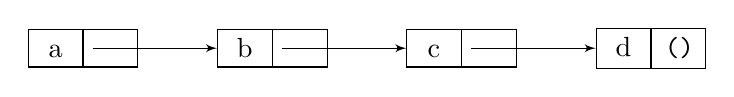
\begin{tikzpicture}[start chain]

\node[list,on chain] (A1) {a \nodepart{two} \phantom{null}};
\node[list,on chain] (A2) {b \nodepart{two} \phantom{null}};
\node[list,on chain] (A3) {c \nodepart{two} \phantom{null}};
\node[list,on chain] (A4) {d \nodepart{two} \texttt{()}};
  
\pSF{A1}{A2};
\pSF{A2}{A3};
\pSF{A3}{A4};

\end{tikzpicture}
\end{figure}

The cdr of the last pair in a \label{start_s28}\textit{proper list} is the empty list.
Otherwise, the sequence of pairs forms an \label{start_s29}\textit{improper list}.
More formally, the empty list is a proper list, and any pair whose cdr
is a proper list is a proper list.

An improper list is printed in \textit{dotted-pair notation}, with a
period, or \label{start_s30}\label{start_s31}\textit{dot},
preceding the final element of the list.


\begin{alltt}
(cons 'a 'b) \(\Rightarrow\) (a . b)
(cdr '(a . b)) \(\Rightarrow\) b
(cons 'a '(b . c)) \(\Rightarrow\) (a b . c)
\end{alltt}


Because of its printed notation, a pair whose cdr is not a list is
often called a \label{start_s32}\textit{dotted pair}.
Even pairs whose cdrs are lists can be written in dotted-pair
notation, however, although the printer always chooses to write
proper lists without dots.


\texttt{'(a . (b . (c . ()))) \(\Rightarrow\) (a b c)}

The procedure \label{start_s33}\texttt{list} is similar to \texttt{cons}, except that it takes
an arbitrary number of arguments and always builds a proper list.


\begin{alltt}
(list 'a 'b 'c) \(\Rightarrow\) (a b c)
(list 'a) \(\Rightarrow\) (a)
(list) \(\Rightarrow\) ()
\end{alltt}


Section \ref{objects_g109} provides more information on lists and the Scheme
procedures for manipulating them.
This might be a good time to turn to that section and familiarize
yourself with the other procedures given there.


\paragraph{Exercise \label{start_g7}2.2.1}


\label{start_s34}Convert the following arithmetic expressions into Scheme expressions
and evaluate them.


 
 \begin{enumerate}[\it a. ]
\item $1.2 \times (2 - 1/3) + -8.7$
\item $(2/3 + 4/9) \div (5/11 - 4/3)$
\item $1 + 1 \div (2 + 1 \div (1 + 1/2))$
\item $1 \times -2 \times 3 \times -4 \times 5 \times -6 \times 7$
\end{enumerate}




\paragraph{Exercise \label{start_g8}2.2.2}


\label{start_s35}Experiment with the procedures \texttt{+}, \texttt{-}, \texttt{*}, and \texttt{/}
to determine Scheme's rules for the type of value returned by
each when given different types of numeric arguments.




\paragraph{Exercise \label{start_g9}2.2.3}


\label{start_s36}\label{start_EXEXPRVALUE}Determine the values of the following expressions.
Use your Scheme system to verify your answers.


 
 \begin{enumerate}[\it a. ]
\item \texttt{(cons 'car 'cdr)}
\item \texttt{(list 'this '(is silly))}
\item \texttt{(cons 'is '(this silly?))}
\item \texttt{(quote (+ 2 3))}
\item \texttt{(cons '+ '(2 3))}
\item \texttt{(car '(+ 2 3))}
\item \texttt{(cdr '(+ 2 3))}
\item \texttt{cons}
\item \texttt{(quote cons)}
\item \texttt{(quote (quote cons))}
\item \texttt{(car (quote (quote cons)))}
\item \texttt{(+ 2 3)}
\item \texttt{(+ '2 '3)}
\item \texttt{(+ (car '(2 3)) (car (cdr '(2 3))))}
\item \texttt{((car (list + - * /)) 2 3)}
\end{enumerate}




\paragraph{Exercise \label{start_g10}2.2.4}


\label{start_s37}\texttt{(car (car '((a b) (c d))))} yields \texttt{a}.
Determine which compositions of \texttt{car} and \texttt{cdr} applied
to \texttt{((a b) (c d))} yield \texttt{b}, \texttt{c}, and
\texttt{d}.




\paragraph{Exercise \label{start_g11}2.2.5}


\label{start_s38}Write a Scheme expression that evaluates to the following internal
list structure.


\begin{figure}[H]
\centering
%\includegraphics{math/2.eps}
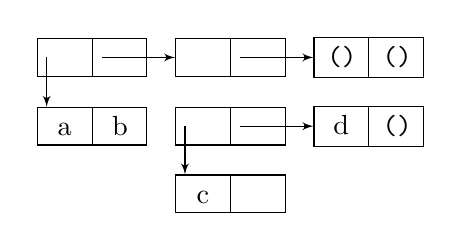
\begin{tikzpicture}

\matrix [row sep = 1em, column sep = 1em]
{
  \node[list] (A1) {\phantom{null} \nodepart{two} \phantom{null}}; & \node[list] (A2) {\phantom{null} \nodepart{two} \phantom{null}}; & \node[list] (A3) {\texttt{()} \nodepart{two} \texttt{()}}; \\
  \node[list] (B1) {a \nodepart{two} b}; & \node[list] (B2) {\phantom{null} \nodepart{two} \phantom{null}}; & \node[list] (B3) {d \nodepart{two} \texttt{()}}; \\
  & \node[list] (C1) {c \nodepart{two} \phantom{null}}; & \\
};
  
\pSF{A1}{A2};
\pSF{A2}{A3};
\pSF{B2}{B3};

\pFF{A1}{B1};
\pFF{B2}{C1};

\end{tikzpicture}
\end{figure}





\paragraph{Exercise \label{start_g12}2.2.6}


\label{start_s39}Draw the internal list structure produced by the expression below.


\texttt{(cons 1 (cons '(2 . ((3) . ())) (cons '(()) (cons 4 5))))}



\paragraph{Exercise \label{start_g13}2.2.7}


\label{start_s40}The behavior of
\texttt{(car (car (car '((a b) (c d)))))} is undefined because
\texttt{(car '((a b) (c d)))} is \texttt{(a b)},
\texttt{(car '(a b))} is \texttt{a},
and \texttt{(car 'a)} is undefined.
Determine all legal compositions of \texttt{car} and \texttt{cdr} applied
to \texttt{((a b) (c d))}.





\paragraph{Exercise \label{start_g14}2.2.8}


\label{start_s41}Try to explain how Scheme expressions are evaluated.
Does your explanation cover the last example in Exercise \hyperref[start_g9]{2.2.3}?




\section{\label{start_g15}\label{start_h3}Evaluating Scheme Expressions\label{start_SECTGSEVALUATING}}



Let's turn to a discussion of how Scheme evaluates the expressions
you type.
We have already established the rules for \label{start_s42}constant objects
such as strings and numbers: the object itself is the value.
You have probably also worked out in your mind a rule for evaluating
\label{start_s43}procedure applications of the form
\texttt{(\textit{procedure} \textit{arg\textsubscript{1}} ... \textit{arg\textsubscript{n}})}.
Here, \texttt{\textit{procedure}} is an expression representing a Scheme procedure,
and \texttt{\textit{arg\textsubscript{1}} ... \textit{arg\textsubscript{n}}} are expressions representing its
arguments.
One possibility is the following.

\begin{itemize}
\item 
Find the value of \texttt{\textit{procedure}}.

\item 
Find the value of \texttt{\textit{arg\textsubscript{1}}}.

\(\vdots\)
\item 
Find the value of \texttt{\textit{arg\textsubscript{n}}}.

\item 
Apply the value of \texttt{\textit{procedure}} to the values
of \texttt{\textit{arg\textsubscript{1}} ... \textit{arg\textsubscript{n}}}.

\end{itemize}


For example, consider the simple procedure application \texttt{(+ 3 4)}.
The value of \texttt{+} is the addition procedure, the value of 3
is the number 3, and the value of 4 is the number 4.
Applying the addition procedure to 3 and 4 yields 7, so our value
is the object 7.


By applying this process at each level, we can find the value of the
nested expression \texttt{(* (+ 3 4) 2)}.
The value of \texttt{*} is the multiplication procedure, the value of
\texttt{(+ 3 4)} we can determine to be the number 7, and the
value of 2 is the number 2.
Multiplying 7 by 2 we get 14, so our answer is 14.


This rule works for procedure applications but not
for
\label{start_s44}\label{start_s45}\texttt{quote} expressions
because the subexpressions of a procedure application are
evaluated, whereas the subexpression of a \texttt{quote} expression is
not.
The evaluation of a \texttt{quote} expression is more similar to the
evaluation of constant objects.
The value of a \texttt{quote} expression of the form
\texttt{(quote \textit{object})}
is simply \texttt{\textit{object}}.


Constant objects, procedure applications, and \texttt{quote} expressions
are only three of the many syntactic forms provided by Scheme.
Fortunately, only a few of the other syntactic forms need to be
understood directly by a Scheme programmer; these are referred to as
\textit{core} syntactic forms.
The remaining syntactic forms are \label{start_s46}\textit{syntactic extensions}
defined, ultimately, in terms of the \label{start_s47}core syntactic forms.
We will discuss the remaining core syntactic forms and a few
syntactic extensions in the remaining sections of this chapter.
Section \ref{further_g50} summarizes the core syntactic forms and introduces
the syntactic extension mechanism.


Before we go on to more syntactic forms and procedures,
two points related to the evaluation of procedure applications
are worthy of note.
\label{start_s48}First, the process given above is
overspecified, in that it requires the subexpressions to be evaluated
from left to right.
That is, \texttt{\textit{procedure}} is evaluated before \texttt{\textit{arg\textsubscript{1}}},
\texttt{\textit{arg\textsubscript{1}}} is evaluated before \texttt{\textit{arg\textsubscript{2}}}, and so on.
This need not be the case.
A Scheme evaluator is free to evaluate the expressions in
any order---left to right, right to left, or any other sequential
order.
In fact, the subexpressions may be evaluated in different orders
for different applications, even in the same implementation.


The second point is that \texttt{\textit{procedure}} is evaluated in the
same way as \texttt{\textit{arg\textsubscript{1}} ... \textit{arg\textsubscript{n}}}.
While \texttt{\textit{procedure}} is often a variable
that names a particular procedure, this need not be the case.
Exercise \hyperref[start_g9]{2.2.3} had you determine
the value of the expression \texttt{((car (list + - * /)) 2 3)}.
Here, \texttt{\textit{procedure}} is \texttt{(car (list + - * /))}.
The value of \texttt{(car (list + - * /))} is the addition procedure,
just as if \texttt{\textit{procedure}} were simply the variable
\texttt{+}.


\paragraph{Exercise \label{start_g16}2.3.1}


\label{start_s49}Write down the steps necessary to evaluate the expression below.


\texttt{((car (cdr (list + - * /))) 17 5)}


\section{\label{start_g17}\label{start_h4}Variables and Let Expressions\label{start_SECTGSIDENTIFIERS}}



\label{start_s50}Suppose \texttt{\textit{expr}} is a Scheme expression that contains
a variable \texttt{\textit{var}}.
Suppose, additionally, that we would like \texttt{\textit{var}} to have the value 
\texttt{\textit{val}} when we evaluate \texttt{\textit{expr}}.
For example, we might like \texttt{x} to have the value 2 when we 
evaluate \texttt{(+ x 3)}.
Or, we might want \texttt{y} to have the value 3 when we evaluate 
\texttt{(+ 2 y)}.
The following examples demonstrate how to do this using Scheme's
\label{start_s51}\texttt{let} syntactic form.


\begin{alltt}
(let ((x 2))
  (+ x 3)) \(\Rightarrow\) 5

(let ((y 3))
  (+ 2 y)) \(\Rightarrow\) 5

(let ((x 2) (y 3))
  (+ x y)) \(\Rightarrow\) 5
\end{alltt}


The \texttt{let} syntactic form includes a list of variable-expression pairs, 
along with a sequence of expressions referred to as the \textit{body} of the
\texttt{let}. 
The general form of a \texttt{let} expression is


\texttt{(let ((\textit{var} \textit{expr}) ...) \textit{body\textsubscript{1}} \textit{body\textsubscript{2}} ...)}

\label{start_s52}We say the variables are \textit{bound} to the
values by the \texttt{let}.
We refer to variables bound by \texttt{let} as
\label{start_s53}\texttt{let}-\textit{bound} variables.


A \texttt{let} expression is often used to simplify an expression that
would contain two identical subexpressions.
Doing so also ensures that the
value of the common subexpression is computed only once.


\begin{alltt}
(+ (* 4 4) (* 4 4)) \(\Rightarrow\) 32

(let ((a (* 4 4))) (+ a a)) \(\Rightarrow\) 32
\end{alltt}


Brackets are often used in place of parentheses to delimit the bindings of
a \texttt{let} expression.


\begin{alltt}
(let ([list1 '(a b c)] [list2 '(d e f)])
  (cons (cons (car list1)
              (car list2))
        (cons (car (cdr list1))
              (car (cdr list2))))) \(\Rightarrow\) ((a . d) b . e)
\end{alltt}


Scheme treats forms enclosed in brackets just like forms enclosed in
parentheses.
An open bracket must be matched by a close bracket, and an open
parenthesis must be matched by a close parenthesis.
We use brackets for \texttt{let} (and, as we'll see, several other
standard syntactic forms) to improve readability, especially when we might
otherwise have two or more consecutive open parentheses.


Since expressions in the first position of a procedure application
are evaluated no differently from other expressions, a \texttt{let}-bound
variable may be used there as well.


\begin{alltt}
(let ([f +])
  (f 2 3)) \(\Rightarrow\) 5

(let ([f +] [x 2])
  (f x 3)) \(\Rightarrow\) 5

(let ([f +] [x 2] [y 3])
  (f x y)) \(\Rightarrow\) 5
\end{alltt}


The variables bound by \texttt{let} are visible only within the body of 
the \texttt{let}.


\begin{alltt}
(let ([+ *])
  (+ 2 3)) \(\Rightarrow\) 6

(+ 2 3) \(\Rightarrow\) 5
\end{alltt}


This is fortunate, because we would not want the
value of \texttt{+} to be the multiplication procedure everywhere.


It is possible to nest \texttt{let} expressions.


\begin{alltt}
(let ([a 4] [b -3])
  (let ([a-squared (* a a)]
        [b-squared (* b b)])
    (+ a-squared b-squared))) \(\Rightarrow\) 25
\end{alltt}


When nested \texttt{let} expressions bind the same variable, only the 
binding created by the inner \texttt{let} is visible within its body.


\begin{alltt}
(let ([x 1])
  (let ([x (+ x 1)])
    (+ x x))) \(\Rightarrow\) 4
\end{alltt}


The outer \texttt{let} expression binds \texttt{x} to 1 within its
body, which is the second \texttt{let} expression.
The inner \texttt{let} expression binds \texttt{x} to \texttt{(+ x 1)} within
its body, which is the expression \texttt{(+ x x)}.
What is the value of \texttt{(+ x 1)}?
Since \texttt{(+ x 1)} appears within the body of the outer \texttt{let}
but not within the body of the inner \texttt{let}, the value of \texttt{x}
must be 1 and hence the value of \texttt{(+ x 1)} is 2.
What about \texttt{(+ x x)}?
It appears within the body of both \texttt{let} expressions.
Only the inner binding for \texttt{x} is visible, so \texttt{x} is 2
and \texttt{(+ x x)} is 4.



\label{start_s54}The inner binding for \texttt{x} is said to \textit{shadow} the
outer binding.
A \texttt{let}-bound variable is visible everywhere within the body of its
\texttt{let} expression except where it is shadowed.
The region where a variable binding is visible is called its
\label{start_s55}\textit{scope}.
The scope of the first \texttt{x} in the example above is the body of
the outer \texttt{let} expression minus the body of the inner \texttt{let}
expression, where it is shadowed by the second \texttt{x}.
This form of scoping is referred to as \label{start_s56}\textit{lexical scoping},
since the scope of each binding can be determined by a straightforward
textual analysis of the program.



Shadowing may be avoided by choosing different names
for variables.
The expression above could be rewritten so that the variable bound
by the inner \texttt{let} is \texttt{new-x}.


\begin{alltt}
(let ([x 1])
  (let ([new-x (+ x 1)])
    (+ new-x new-x))) \(\Rightarrow\) 4
\end{alltt}


Although choosing different names can sometimes prevent confusion,
shadowing can help prevent the accidental use of an
``old'' value.
For example, with the original version of the preceding example,
it would be impossible for us to mistakenly refer to the outer \texttt{x}
within the body of the inner \texttt{let}.


\paragraph{Exercise \label{start_g18}2.4.1}


\label{start_s57}Rewrite the following expressions, using \texttt{let} to remove common
subexpressions and to improve the structure of the code.
Do not perform any algebraic simplifications.


 
 \begin{enumerate}[\it a. ]
\item \texttt{(+ (- (* 3 a) b) (+ (* 3 a) b))}
\item \texttt{(cons (car (list a b c)) (cdr (list a b c)))}
\end{enumerate}




\paragraph{Exercise \label{start_g19}2.4.2}


\label{start_s58}Determine the value of the following expression.
Explain how you derived this value.


\begin{alltt}
(let ([x 9])
  (* x
     (let ([x (/ x 3)])
       (+ x x))))
\end{alltt}



\paragraph{Exercise \label{start_g20}2.4.3}


\label{start_s59}Rewrite the following expressions to give unique names to each different
\texttt{let}-bound variable so that none of the variables is shadowed.
Verify that the value of your expression is the same as that of the
original expression.


 
 \begin{enumerate}[\it a. ]
\item 
\begin{alltt}
(let ([x 'a] [y 'b])
  (list (let ([x 'c]) (cons x y))
        (let ([y 'd]) (cons x y))))
\end{alltt}

\item 
\begin{alltt}
(let ([x '((a b) c)])
  (cons (let ([x (cdr x)])
          (car x))
        (let ([x (car x)])
          (cons (let ([x (cdr x)])
                  (car x))
                (cons (let ([x (car x)])
                        x)
                      (cdr x))))))
\end{alltt}

\end{enumerate}




\section{\label{start_g21}\label{start_h5}Lambda Expressions\label{start_SECTGSLAMBDA}}



In the expression \texttt{(let ([x (* 3 4)]) (+ x x))}, the variable
\texttt{x} is bound to the value of \texttt{(* 3 4)}.
What if we would like the value of \texttt{(+ x x)} where \texttt{x} is
bound to the value of \texttt{(/ 99 11)}?
Where \texttt{x} is bound to the value of \texttt{(- 2 7)}?
In each case we need a different \texttt{let} expression.
When the body of the \texttt{let} is complicated, however, having to
repeat it can be inconvenient.


Instead, we can use the syntactic form \label{start_s60}\texttt{lambda} to create a new
\label{start_s61}procedure that has \texttt{x} as a parameter and has the same
body as the \texttt{let} expression.


\texttt{(lambda (x) (+ x x)) \(\Rightarrow\) \#{}\textless{}procedure\textgreater{}}

The general form of a \texttt{lambda} expression is


\texttt{(lambda (\textit{var} ...) \textit{body\textsubscript{1}} \textit{body\textsubscript{2}} ...)}

The variables \texttt{\textit{var} ...} are the \label{start_s62}\textit{formal parameters}
of the procedure, and the sequence of expressions
\texttt{\textit{body\textsubscript{1}} \textit{body\textsubscript{2}} ...} is its body.
(Actually, the true general form is somewhat more general than this,
as you will see later.)


A procedure is just as much an object as a number, string, symbol,
or pair.
It does not have any meaningful printed representation as
far as Scheme is concerned, however, so this book uses the notation
\texttt{\#{}\textless{}procedure\textgreater{}} to show that the value of an expression is a
procedure.


The most common operation to perform on a procedure is to apply it
to one or more values.


\texttt{((lambda (x) (+ x x)) (* 3 4)) \(\Rightarrow\) 24}

This is no different from any other \label{start_s63}procedure application.
The procedure is the value of \texttt{(lambda (x) (+ x x))}, and the
only argument is the value of \texttt{(* 3 4)}, or 12.
The argument values, or \label{start_s64}\textit{actual parameters}, are bound to the
formal parameters within the body of the \texttt{lambda} expression
in the same way as \texttt{let}-bound variables are bound to their values.
In this case, \texttt{x} is bound to 12, and
the value of \texttt{(+ x x)} is 24.
Thus, the result of applying the procedure to the value 12 is 24.


Because procedures are objects, we can establish
a procedure as the value of a variable and use the procedure more
than once.\label{start_s65}


\begin{alltt}
(let ([double (lambda (x) (+ x x))])
  (list (double (* 3 4))
        (double (/ 99 11))
        (double (- 2 7)))) \(\Rightarrow\) (24 18 -10)
\end{alltt}


Here, we establish a binding for \texttt{double} to a procedure, then
use this procedure to double three different values.


The procedure expects its actual parameter to be a number, since
it passes the actual parameter on to \texttt{+}.
In general, the actual parameter may be any sort of object.
Consider, for example, a similar procedure that uses \texttt{cons}
instead of \texttt{+}.\label{start_s66}


\begin{alltt}
(let ([double-cons (lambda (x) (cons x x))])
  (double-cons 'a)) \(\Rightarrow\) (a . a)
\end{alltt}


Noting the similarity between \texttt{double} and \texttt{double-cons},
you should not be surprised to learn that they may be collapsed
into a single procedure by adding an additional argument.


\begin{alltt}
(let ([double-any (lambda (f x) (f x x))])
  (list (double-any + 13)
        (double-any cons 'a))) \(\Rightarrow\) (26 (a . a))
\end{alltt}


This demonstrates that procedures may accept more than
one argument and that arguments passed to a procedure may
themselves be procedures.


As with \texttt{let} expressions, \texttt{lambda} expressions become
somewhat more interesting when they are nested within other
\texttt{lambda} or \texttt{let} expressions.


\begin{alltt}
(let ([x 'a])
  (let ([f (lambda (y) (list x y))])
    (f 'b))) \(\Rightarrow\) (a b)
\end{alltt}


The occurrence of \texttt{x} within the \texttt{lambda} expression
refers to the \texttt{x} outside the \texttt{lambda} that is bound by
the outer \texttt{let} expression.
The variable \texttt{x} is said to \label{start_s67}\textit{occur free}
in the \texttt{lambda} expression or to be a
\label{start_s68}\textit{free variable} of the \texttt{lambda} expression.
The variable \texttt{y} does not occur free in the \texttt{lambda}
expression since it is bound by the \texttt{lambda} expression.
A variable that occurs free in a \texttt{lambda} expression
should be bound, e.g., by an enclosing \texttt{lambda} or \texttt{let}
expression, unless the variable is (like the names of primitive
procedures) bound outside of the expression, as we discuss in
the following section.


What happens when the procedure is applied somewhere outside
the scope of the bindings for variables that occur free
within the procedure, as in the following expression?


\begin{alltt}
(let ([f (let ([x 'sam])
           (lambda (y z) (list x y z)))])
  (f 'i 'am)) \(\Rightarrow\) (sam i am)
\end{alltt}


The answer is that the same bindings that were in effect when
the procedure was created are in effect again when the procedure
is applied.
This is true even if another binding for \texttt{x}
is visible where the procedure is applied.


\begin{alltt}
(let ([f (let ([x 'sam])
           (lambda (y z) (list x y z)))])
  (let ([x 'not-sam])
    (f 'i 'am))) \(\Rightarrow\) (sam i am)
\end{alltt}


In both cases, the value of \texttt{x} within the procedure named
\texttt{f} is \texttt{sam}.



Incidentally, a \texttt{let} expression is nothing more than the
direct application of a \texttt{lambda} expression to a set of
argument expressions.
For example, the two expressions below are equivalent.


\texttt{(let ([x 'a]) (cons x x))} \(\equiv\) \texttt{((lambda (x) (cons x x)) 'a)}


In fact, a \label{start_s69}\texttt{let} expression is a syntactic extension defined
in terms of \texttt{lambda} and procedure application, which are
both core syntactic forms.
In general, any expression of the form


\texttt{(let ((\textit{var} \textit{expr}) ...) \textit{body\textsubscript{1}} \textit{body\textsubscript{2}} ...)}

is equivalent to the following.


\begin{alltt}
((lambda (\textit{var} ...) \textit{body\textsubscript{1}} \textit{body\textsubscript{2}} ...)
 \textit{expr} ...)
\end{alltt}


See Section \ref{further_g50} for more about core forms and syntactic
extensions.


As mentioned above, the general form of
\label{start_s70}\label{start_s71}\texttt{lambda} is a bit
more complicated than the form we saw earlier, in that the
formal parameter specification, \texttt{(\textit{var} ...)}, need not be a proper list,
or indeed even a list at all.
The formal parameter specification can be in any of the following three forms:

\begin{itemize}
\item 
a proper list of variables, \texttt{(\textit{var\textsubscript{1}} ... \textit{var\textsubscript{n}})}, such
as we have already seen,

\item 
a single variable, \texttt{\textit{var\textsubscript{r}}}, or

\item 
an improper list of variables,
\texttt{(\textit{var\textsubscript{1}} ... \textit{var\textsubscript{n}} . \textit{var\textsubscript{r}})}.

\end{itemize}


In the first case, exactly \textit{n} actual parameters must
be supplied, and
each variable is bound to the corresponding actual parameter.
In the second, any number of actual parameters is valid; all of the
actual parameters
are put into a single list and the single variable is bound to this
list.
The third case is a hybrid of the first two cases.
At least \textit{n} actual parameters must be supplied.
The variables \texttt{\textit{var\textsubscript{1}} ... \textit{var\textsubscript{n}}}
are bound to the corresponding actual parameters,
and the variable \texttt{\textit{var\textsubscript{r}}} is bound to a list containing
the remaining actual parameters.
In the second and third cases, \texttt{\textit{var\textsubscript{r}}} is sometimes referred to
as a ``rest'' parameter because it holds the rest of the actual
parameters beyond those that are individually named.


Let's consider a few examples to help clarify the more general
syntax of \texttt{lambda} expressions.


\begin{alltt}
(let ([f (lambda x x)])
  (f 1 2 3 4)) \(\Rightarrow\) (1 2 3 4)

(let ([f (lambda x x)])
  (f)) \(\Rightarrow\) ()

(let ([g (lambda (x . y) (list x y))])
  (g 1 2 3 4)) \(\Rightarrow\) (1 (2 3 4))

(let ([h (lambda (x y . z) (list x y z))])
  (h 'a 'b 'c 'd)) \(\Rightarrow\) (a b (c d))
\end{alltt}


In the first two examples, the procedure named \texttt{f} accepts any
number of arguments.
These arguments are automatically formed into a list to which the
variable \texttt{x} is bound; the value of \texttt{f} is this list.
In the first example, the arguments are 1, 2, 3,
and 4, so the answer is \texttt{(1 2 3 4)}.
In the second, there are no arguments, so the answer is the empty
list \texttt{()}.
The value of the procedure named \texttt{g} in the third example
is a list whose first element is the first argument and whose
second element is a list containing the remaining arguments.
The procedure named \texttt{h} is similar but separates out the
second argument.
While \texttt{f} accepts any number of arguments, \texttt{g} must receive
at least one and \texttt{h} must receive at least two.


\paragraph{Exercise \label{start_g22}2.5.1}


\label{start_s72}Determine the values of the expressions below.


 
 \begin{enumerate}[\it a. ]
\item 
\begin{alltt}
(let ([f (lambda (x) x)])
  (f 'a))
\end{alltt}

\item 
\begin{alltt}
(let ([f (lambda x x)])
  (f 'a))
\end{alltt}

\item 
\begin{alltt}
(let ([f (lambda (x . y) x)])
  (f 'a))
\end{alltt}

\item 
\begin{alltt}
(let ([f (lambda (x . y) y)])
  (f 'a))
\end{alltt}

\end{enumerate}




\paragraph{Exercise \label{start_g23}2.5.2}


\label{start_s73}How might the primitive procedure \texttt{list} be defined?




\paragraph{Exercise \label{start_g24}2.5.3}


\label{start_s74}List the variables that \label{start_s75}occur free in each of the \texttt{lambda}
expressions below.
Do not omit variables that name primitive procedures such as
\texttt{+} or \texttt{cons}.


 
 \begin{enumerate}[\it a. ]
\item \texttt{(lambda (f x) (f x))}
\item \texttt{(lambda (x) (+ x x))}
\item \texttt{(lambda (x y) (f x y))}
\item 
\begin{alltt}
(lambda (x)
  (cons x (f x y)))
\end{alltt}

\item 
\begin{alltt}
(lambda (x)
  (let ([z (cons x y)])
    (x y z)))
\end{alltt}

\item 
\begin{alltt}
(lambda (x)
  (let ([y (cons x y)])
    (x y z)))
\end{alltt}

\end{enumerate}




\section{\label{start_g25}\label{start_h6}Top-Level Definitions\label{start_SECTGSTOPLEVEL}}



\label{start_s76}The \label{start_s77}variables bound by \texttt{let} and \texttt{lambda}
expressions are not visible outside the bodies of these expressions.
Suppose you have created an object, perhaps a procedure, that must
be accessible anywhere, like \texttt{+} or \texttt{cons}.
What you need is a \textit{top-level definition}, which may be established
with \label{start_s78}\texttt{define}.
Top-level definitions, which are supported by most interactive Scheme
systems, are visible in every expression you enter,
except where shadowed by another binding.


Let's establish a top-level definition of the \label{start_s79}\texttt{double-any}
procedure of the last section.


\begin{alltt}
(define double-any
  (lambda (f x)
    (f x x)))
\end{alltt}


The variable \texttt{double-any} now has the same status as \texttt{cons}
or the name of any other primitive procedure.
We can use \texttt{double-any} as if it were a primitive procedure.


\begin{alltt}
(double-any + 10) \(\Rightarrow\) 20
(double-any cons 'a) \(\Rightarrow\) (a . a)
\end{alltt}


A top-level definition may be established for any object, not just
for procedures.


\begin{alltt}
(define sandwich "peanut-butter-and-jelly")

sandwich \(\Rightarrow\) "peanut-butter-and-jelly"
\end{alltt}


\label{start_s80}Most often, though, top-level definitions are
used for procedures.


\label{start_s81}As suggested above, top-level definitions may be shadowed
by \texttt{let} or \texttt{lambda} bindings.


\begin{alltt}
(define xyz '(x y z))
(let ([xyz '(z y x)])
  xyz) \(\Rightarrow\) (z y x)
\end{alltt}


Variables with top-level definitions act almost as if they were bound
by a \texttt{let} expression enclosing all of the expressions you type.


\label{start_defn_list}Given only the simple tools you have read about up to this point,
it is already possible to define some of the primitive procedures
provided by Scheme and described later in this book.
If you completed the exercises from the last section, you should
already know how to define \label{start_s82}\texttt{list}.


\texttt{(define list (lambda x x))}

Also, Scheme provides the abbreviations \label{start_s83}\texttt{cadr} and \label{start_s84}\texttt{cddr} for
the compositions of \texttt{car} with \texttt{cdr} and \texttt{cdr} with \texttt{cdr}.
That is, \texttt{(cadr \textit{list})} is equivalent to
\texttt{(car (cdr \textit{list}))}, and, similarly,
\texttt{(cddr \textit{list})} is equivalent to
\texttt{(cdr (cdr \textit{list}))}.
They are easily defined as follows.


\begin{alltt}
(define cadr
  (lambda (x)
    (car (cdr x))))

(define cddr
  (lambda (x)
    (cdr (cdr x))))
\end{alltt}


\begin{alltt}
(cadr '(a b c)) \(\Rightarrow\) b
(cddr '(a b c)) \(\Rightarrow\) (c)
\end{alltt}


Any definition \texttt{(define \textit{var} \textit{expr})} where \texttt{\textit{expr}} is a
\texttt{lambda} expression can be written in a shorter form that suppresses
the \texttt{lambda}.
The exact syntax depends upon the format of the \texttt{lambda} expression's
formal parameter specifier, i.e., whether it is a proper list of
variables, a single variable, or an improper list of variables.
A definition of the form


\begin{alltt}
(define \textit{var\textsubscript{0}}
  (lambda (\textit{var\textsubscript{1}} ... \textit{var\textsubscript{n}})
    \textit{e\textsubscript{1}} \textit{e\textsubscript{2}} ...))
\end{alltt}


may be abbreviated


\begin{alltt}
(define (\textit{var\textsubscript{0}} \textit{var\textsubscript{1}} ... \textit{var\textsubscript{n}})
  \textit{e\textsubscript{1}} \textit{e\textsubscript{2}} ...)
\end{alltt}


while


\begin{alltt}
(define \textit{var\textsubscript{0}}
  (lambda \textit{var\textsubscript{r}}
    \textit{e\textsubscript{1}} \textit{e\textsubscript{2}} ...))
\end{alltt}


may be abbreviated


\begin{alltt}
(define (\textit{var\textsubscript{0}} . \textit{var\textsubscript{r}})
  \textit{e\textsubscript{1}} \textit{e\textsubscript{2}} ...)
\end{alltt}


and


\begin{alltt}
(define \textit{var\textsubscript{0}}
  (lambda (\textit{var\textsubscript{1}} ... \textit{var\textsubscript{n}} . \textit{var\textsubscript{r}})
    \textit{e\textsubscript{1}} \textit{e\textsubscript{2}} ...))
\end{alltt}


may be abbreviated


\begin{alltt}
(define (\textit{var\textsubscript{0}} \textit{var\textsubscript{1}} ... \textit{var\textsubscript{n}} . \textit{var\textsubscript{r}})
  \textit{e\textsubscript{1}} \textit{e\textsubscript{2}} ...)
\end{alltt}


For example, the definitions of \label{start_s85}\texttt{cadr} and \label{start_s86}\texttt{list} might be written
as follows.


\begin{alltt}
(define (cadr x)
  (car (cdr x)))

(define (list . x) x)
\end{alltt}


This book does not often employ this alternative syntax.
Although it is shorter, it tends to mask the reality that procedures
are not intimately tied to variables, or names, as they are in many
other languages.
This syntax is often referred to, somewhat pejoratively,
as the \label{start_s87}``defun'' syntax for \texttt{define}, after the
\texttt{defun} form provided by Lisp languages in which procedures are more
closely tied to their names.


Top-level definitions make it easier for us to experiment with a
procedure interactively
because we need not retype the procedure each time it is used.
Let's try defining a somewhat more complicated variation of \texttt{double-any},
one that turns an ``ordinary'' two-argument procedure into a ``doubling''
one-argument \label{start_s88}procedure.


\begin{alltt}
(define doubler
  (lambda (f)
    (lambda (x) (f x x))))
\end{alltt}

\texttt{doubler} accepts one argument, \texttt{f}, which must be a
procedure that accepts two arguments.
The procedure returned by \texttt{doubler} accepts one argument, which
it uses for both arguments in an application of \texttt{f}.
We can define, with \texttt{doubler}, the simple
\label{start_s89}\texttt{double} and
\label{start_s90}\texttt{double-cons} procedures
of the last section.

\begin{alltt}
(define double (doubler +))
(double 13/2) \(\Rightarrow\) 13

(define double-cons (doubler cons))
(double-cons 'a) \(\Rightarrow\) (a . a)
\end{alltt}


We can also define \texttt{double-any} with \texttt{doubler}.


\begin{alltt}
(define double-any
  (lambda (f x)
    ((doubler f) x)))
\end{alltt}


Within \texttt{double} and
\texttt{double-cons}, \texttt{f} has the appropriate value, i.e., \texttt{+}
or \texttt{cons}, even though the procedures are clearly applied outside the
scope of \texttt{f}.


What happens if you attempt to use a variable that is not bound by a
\texttt{let} or \texttt{lambda} expression and that does not have a top-level
definition?
Try using the variable \texttt{i-am-not-defined} to see what happens.


\texttt{(i-am-not-defined 3)}

Most Scheme systems print a message
indicating that an unbound- or undefined-variable exception
has occurred.


The system should not, however, complain
about the appearance of an undefined variable
within a \texttt{lambda} expression, until and unless the resulting procedure
is applied.
The following should \textit{not} cause an exception, even though we have not yet
established a top-level definition of \texttt{proc2}.


\begin{alltt}
(define proc1
  (lambda (x y)
    (proc2 y x)))
\end{alltt}


If you try to apply \texttt{proc1} before defining \texttt{proc2}, you should get
a undefined exception message.
Let's give \texttt{proc2} a top-level definition and try \texttt{proc1}.


\begin{alltt}
(define proc2 cons)
(proc1 'a 'b) \(\Rightarrow\) (b . a)
\end{alltt}


When you define \texttt{proc1}, the system accepts your promise to define
\texttt{proc2}, and does not complain unless you use \texttt{proc1} before
defining \texttt{proc2}.
This allows you to define procedures in any order you please.
This is especially useful when you are trying to organize a file full of
procedure definitions in a way that makes your program more readable.
It is necessary when two procedures defined at top level depend upon
each other; we will see some examples of this later.


\paragraph{Exercise \label{start_g26}2.6.1}


\label{start_s91}What would happen if you were to type


\texttt{(double-any double-any double-any)}

given the definition of \texttt{double-any} from the beginning of this
section?




\paragraph{Exercise \label{start_g27}2.6.2}


\label{start_s92}A more elegant (though possibly less efficient) way to define \label{start_s93}\texttt{cadr}
and \label{start_s94}\texttt{cddr} than given in this
section is to define a procedure that composes two procedures to create
a third.
Write the procedure \label{start_s95}\texttt{compose}, such that
\texttt{(compose \textit{p\textsubscript{1}} \textit{p\textsubscript{2}})} is the composition of
\texttt{\textit{p\textsubscript{1}}} and \texttt{\textit{p\textsubscript{2}}} (assuming both take one argument).
That is, \texttt{(compose \textit{p\textsubscript{1}} \textit{p\textsubscript{2}})} should return a new
procedure of one argument that applies \texttt{\textit{p\textsubscript{1}}} to the result of
applying \texttt{\textit{p\textsubscript{2}}} to the argument.
Use \texttt{compose} to define \texttt{cadr} and \texttt{cddr}.




\paragraph{Exercise \label{start_g28}2.6.3}


\label{start_s96}Scheme also provides
\label{start_s97}\texttt{caar}, \texttt{cdar}, \texttt{caaar}, \texttt{caadr},
and so on, with any combination of up to four \texttt{a}'s (representing
\texttt{car}) and \texttt{d}'s (representing \texttt{cdr}) between the \texttt{c}
and the \texttt{r} (see Section \ref{objects_g109}).
Define each of these with the \texttt{compose} procedure of the preceding
exercise.




\section{\label{start_g29}\label{start_h7}Conditional Expressions\label{start_SECTGSCONDITIONALS}}



So far we have considered expressions that perform a given task
unconditionally.
Suppose that we wish to write the procedure \label{start_s98}\texttt{abs}.
If its argument \textit{x} is negative, \texttt{abs}
returns -\textit{x}; otherwise, it returns \textit{x}.
The most straightforward way to write \texttt{abs} is to determine
whether the argument is negative and if so negate it, using the
\label{start_s99}\texttt{if} syntactic form.



\begin{alltt}
(define abs
  (lambda (n)
    (if (\textless{} n 0)
        (- 0 n)
        n)))

(abs 77) \(\Rightarrow\) 77
(abs -77) \(\Rightarrow\) 77
\end{alltt}


An \texttt{if} expression has the form
\texttt{(if \textit{test} \textit{consequent} \textit{alternative})}, where
\texttt{\textit{consequent}} is the expression to evaluate if \texttt{\textit{test}} is true
and 
\texttt{\textit{alternative}} is the expression to evaluate if \texttt{\textit{test}} is false.
In the expression above, \texttt{\textit{test}} is \texttt{(\textless{} n 0)}, \texttt{\textit{consequent}}
is \texttt{(- 0 n)}, and \texttt{\textit{alternative}} is \texttt{n}.


The procedure \texttt{abs} could be written in a variety of other ways.
Any of the following are valid definitions of \texttt{abs}.


\begin{alltt}
(define abs
  (lambda (n)
    (if (\textgreater{}= n 0)
        n
        (- 0 n))))

(define abs
  (lambda (n)
    (if (not (\textless{} n 0))
        n
        (- 0 n))))

(define abs
  (lambda (n)
    (if (or (\textgreater{} n 0) (= n 0))
        n
        (- 0 n))))

(define abs
  (lambda (n)
    (if (= n 0)
        0
        (if (\textless{} n 0)
            (- 0 n)
            n))))

(define abs
  (lambda (n)
    ((if (\textgreater{}= n 0) + -)
     0
     n)))
\end{alltt}


The first of these definitions asks if \texttt{n} is greater
than or equal to zero, inverting the test.
The second asks if \texttt{n} is not less than zero, using the procedure
\label{start_s100}\texttt{not} with \texttt{\textless{}}.
The third asks if \texttt{n} is greater than zero or \texttt{n} is equal to
zero, using the syntactic form \label{start_s101}\texttt{or}.
The fourth treats zero separately, though there is no benefit in doing so.
The fifth is somewhat tricky; \texttt{n} is either added to or subtracted from
zero, depending upon whether \texttt{n} is greater than or equal to zero.


Why is \label{start_s102}\texttt{if} a syntactic form and not a procedure?
In order to answer this, let's revisit the definition of
\texttt{reciprocal} from the first section of this chapter.


\begin{alltt}
(define reciprocal
  (lambda (n)
    (if (= n 0)
        "oops!"
        (/ 1 n))))
\end{alltt}


The second argument to the division procedure should not be zero,
since the result is mathematically undefined.
Our definition of \texttt{reciprocal} avoids this problem by
testing for zero before dividing.
Were \texttt{if} a procedure, its arguments (including \texttt{(/ 1 n)})
would be evaluated before it had a chance to choose between the
consequent and alternative.
Like \texttt{quote}, which does not evaluate its only subexpression,
\texttt{if} does not evaluate all of its subexpressions and so cannot
be a procedure.


The syntactic form \label{start_s103}\texttt{or} operates in a manner similar to \texttt{if}.
The general form of an \texttt{or} expression is \texttt{(or \textit{expr} ...)}.
If there are no subexpressions, i.e., the expression is simply \texttt{(or)},
the value is false.
Otherwise, each \texttt{\textit{expr}} is evaluated in turn until either (a) one of
the expressions evaluates to true or (b) no more expressions are left.
In case (a), the value is true; in case (b), the value is false.


To be more precise, in case (a), the value of the \texttt{or}
expression is the value of the last subexpression evaluated.
This clarification is necessary because there are many possible true
values.
Usually, the value of a test expression is one of the two objects
\label{start_s104}\texttt{\#{}t}, for true, or \label{start_s105}\texttt{\#{}f}, for false.


\begin{alltt}
(\textless{} -1 0) \(\Rightarrow\) \#{}t
(\textgreater{} -1 0) \(\Rightarrow\) \#{}f
\end{alltt}


Every Scheme object, however, is considered to be either \label{start_s106}true
or \label{start_s107}false by conditional expressions and by
the procedure \texttt{not}.
Only \texttt{\#{}f} is considered false; all other objects are considered
true.


\begin{alltt}
(if \#{}t 'true 'false) \(\Rightarrow\) true
(if \#{}f 'true 'false) \(\Rightarrow\) false
(if '() 'true 'false) \(\Rightarrow\) true
(if 1 'true 'false) \(\Rightarrow\) true
(if '(a b c) 'true 'false) \(\Rightarrow\) true

(not \#{}t) \(\Rightarrow\) \#{}f
(not "false") \(\Rightarrow\) \#{}f
(not \#{}f) \(\Rightarrow\) \#{}t

(or) \(\Rightarrow\) \#{}f
(or \#{}f) \(\Rightarrow\) \#{}f
(or \#{}f \#{}t) \(\Rightarrow\) \#{}t
(or \#{}f 'a \#{}f) \(\Rightarrow\) a
\end{alltt}


The \label{start_s108}\texttt{and} syntactic form is similar in form to \texttt{or}, but an
\texttt{and} expression is true if all its subexpressions are true, and
false otherwise.
In the case where there are no subexpressions, i.e., the expression is
simply \texttt{(and)}, the value is true.
Otherwise, the subexpressions are evaluated in turn until either
no more subexpressions are left or the value of a subexpression is
false.
The value of the \texttt{and} expression
is the value of the last subexpression evaluated.


Using \texttt{and}, we can define a slightly different version of
\label{start_s109}\texttt{reciprocal}.


\begin{alltt}
(define reciprocal
  (lambda (n)
    (and (not (= n 0))
         (/ 1 n))))

(reciprocal 3) \(\Rightarrow\) 1/3
(reciprocal 0.5) \(\Rightarrow\) 2.0
(reciprocal 0) \(\Rightarrow\) \#{}f
\end{alltt}


In this version, the value is \texttt{\#{}f} if \texttt{n} is zero and \texttt{1/n} otherwise.


The procedures \texttt{=}, \texttt{\textless{}}, \texttt{\textgreater{}}, \texttt{\textless{}=}, and \texttt{\textgreater{}=} are
called \label{start_s110}\textit{predicates}.
A predicate is a procedure that answers a specific question about its
arguments and returns one of the two values \texttt{\#{}t} or \texttt{\#{}f}.
The names of most predicates end with a
\label{start_s111}\label{start_s112}question mark ( \texttt{?} ); the
common numeric procedures listed above are exceptions to this
rule.
Not all predicates require numeric arguments, of course.
The predicate \label{start_s113}\texttt{null?} returns true if its argument is the empty
list \texttt{()} and false otherwise.


\begin{alltt}
(null? '()) \(\Rightarrow\) \#{}t
(null? 'abc) \(\Rightarrow\) \#{}f
(null? '(x y z)) \(\Rightarrow\) \#{}f
(null? (cdddr '(x y z))) \(\Rightarrow\) \#{}t
\end{alltt}


The procedure \label{start_s114}\texttt{cdr} must not be passed anything other than a pair,
and an exception is raised when this happens.
Common Lisp, however, defines \texttt{(cdr '())} to be \texttt{()}.
The following procedure, \label{start_s115}\texttt{lisp-cdr}, is 
defined using \texttt{null?} to return
\texttt{()} if its argument is \texttt{()}.


\begin{alltt}
(define lisp-cdr
  (lambda (x)
    (if (null? x)
        '()
        (cdr x))))

(lisp-cdr '(a b c)) \(\Rightarrow\) (b c)
(lisp-cdr '(c)) \(\Rightarrow\) ()
(lisp-cdr '()) \(\Rightarrow\) ()
\end{alltt}


Another useful predicate is \label{start_s116}\texttt{eqv?}, which
requires two arguments.
If the two arguments are equivalent, \texttt{eqv?} returns true.
Otherwise, \texttt{eqv?} returns false.


\begin{alltt}
(eqv? 'a 'a) \(\Rightarrow\) \#{}t
(eqv? 'a 'b) \(\Rightarrow\) \#{}f
(eqv? \#{}f \#{}f) \(\Rightarrow\) \#{}t
(eqv? \#{}t \#{}t) \(\Rightarrow\) \#{}t
(eqv? \#{}f \#{}t) \(\Rightarrow\) \#{}f
(eqv? 3 3) \(\Rightarrow\) \#{}t
(eqv? 3 2) \(\Rightarrow\) \#{}f
(let ([x "Hi Mom!"])
  (eqv? x x)) \(\Rightarrow\) \#{}t
(let ([x (cons 'a 'b)])
  (eqv? x x)) \(\Rightarrow\) \#{}t
(eqv? (cons 'a 'b) (cons 'a 'b)) \(\Rightarrow\) \#{}f
\end{alltt}


As you can see, \texttt{eqv?} returns true if the arguments are the same
symbol, boolean, number, pair, or string.
Two pairs are not the same by \texttt{eqv?} if they are created by different
calls to \texttt{cons}, even if they have the same contents.
Detailed equivalence rules for \texttt{eqv?} are given in Section \ref{objects_g108}.


Scheme also provides a set
of \label{start_s117}\textit{type predicates} that return true
or false depending on the type of the object, e.g., \label{start_s118}\texttt{pair?},
\label{start_s119}\texttt{symbol?}, \label{start_s120}\texttt{number?}, and \label{start_s121}\texttt{string?}.
The predicate \label{start_s122}\texttt{pair?}, for example, returns true only if its argument
is a pair.


\begin{alltt}
(pair? '(a . c)) \(\Rightarrow\) \#{}t
(pair? '(a b c)) \(\Rightarrow\) \#{}t
(pair? '()) \(\Rightarrow\) \#{}f
(pair? 'abc) \(\Rightarrow\) \#{}f
(pair? "Hi Mom!") \(\Rightarrow\) \#{}f
(pair? 1234567890) \(\Rightarrow\) \#{}f
\end{alltt}


Type predicates are useful for deciding if the argument passed to a
procedure is of the appropriate type.
For example, the following version of \label{start_s123}\texttt{reciprocal} checks first to
see that its argument is a number before testing against zero or
performing the division. 


\begin{alltt}
(define reciprocal
  (lambda (n)
    (if (and (number? n) (not (= n 0)))
        (/ 1 n)
        "oops!")))

(reciprocal 2/3) \(\Rightarrow\) 3/2
(reciprocal 'a) \(\Rightarrow\) "oops!"
\end{alltt}


By the way, the code that uses \texttt{reciprocal} must check to see that
the returned value is a number and not a string.
To relieve the caller of this obligation, it is usually preferable
to report the error, using \texttt{assertion-violation},
as follows.


\begin{alltt}
(define reciprocal
  (lambda (n)
    (if (and (number? n) (not (= n 0)))
        (/ 1 n)
        (assertion-violation 'reciprocal
          "improper argument"
          n))))

(reciprocal .25) \(\Rightarrow\) 4.0
(reciprocal 0) \(\Rightarrow\) \textit{exception in reciprocal: improper argument 0}
(reciprocal 'a) \(\Rightarrow\) \textit{exception in reciprocal: improper argument a}
\end{alltt}


The first argument to \texttt{assertion-violation} is a symbol identifying where
the message originates, the second is a string describing the error,
and the third and subsequent arguments are ``irritants'' to be included with
the error message.


Let's look at one more conditional expression, \label{start_s124}\texttt{cond}, that is often
useful in place of \label{start_s125}\texttt{if}.
\texttt{cond} is similar to \texttt{if} except that it allows multiple
test and alternative expressions.
Consider the following definition of \texttt{sign}, which returns
\texttt{-1} for negative inputs,
\texttt{+1} for positive inputs, and
\texttt{0} for zero.


\begin{alltt}
(define sign
  (lambda (n)
    (if (\textless{} n 0)
        -1
        (if (\textgreater{} n 0)
            +1
            0))))
\end{alltt}


\begin{alltt}
(sign -88.3) \(\Rightarrow\) -1
(sign 0) \(\Rightarrow\) 0
(sign 333333333333) \(\Rightarrow\) 1
(* (sign -88.3) (abs -88.3)) \(\Rightarrow\) -88.3
\end{alltt}


The two \texttt{if} expressions may be replaced by a single \texttt{cond}
expression as follows.


\begin{alltt}
(define sign
  (lambda (n)
    (cond
      [(\textless{} n 0) -1]
      [(\textgreater{} n 0) +1]
      [else 0])))
\end{alltt}


A \texttt{cond} expression usually takes the form


\texttt{(cond (\textit{test} \textit{expr}) ... (else \textit{expr}))}

though the \texttt{else} clause may be omitted.
This should be done only when there is no possibility that all the tests
will fail, as in the new version of \texttt{sign} below.


\begin{alltt}
(define sign
  (lambda (n)
    (cond
      [(\textless{} n 0) -1]
      [(\textgreater{} n 0) +1]
      [(= n 0) 0])))
\end{alltt}


These definitions of \texttt{sign} do not depend on the order in which the
tests are performed, since only one of the tests can be true for any
value of \texttt{n}.
The following procedure computes the tax on a given amount of income in
a progressive tax system with breakpoints at 10,000, 20,000, and 30,000
dollars.


\begin{alltt}
(define income-tax
  (lambda (income)
    (cond
      [(\textless{}= income 10000) (* income .05)]
      [(\textless{}= income 20000) (+ (* (- income 10000) .08) 500.00)]
      [(\textless{}= income 30000) (+ (* (- income 20000) .13) 1300.00)]
      [else (+ (* (- income 30000) .21) 2600.00)])))
\end{alltt}


\begin{alltt}
(income-tax 5000) \(\Rightarrow\) 250.0
(income-tax 15000) \(\Rightarrow\) 900.0
(income-tax 25000) \(\Rightarrow\) 1950.0
(income-tax 50000) \(\Rightarrow\) 6800.0
\end{alltt}


In this example, the order in which the tests are performed,
left to right (top to bottom), is significant.


\paragraph{Exercise \label{start_g30}2.7.1}


\label{start_s126}Define the predicate \label{start_s127}\texttt{atom?}, which returns true if its argument
is not a pair and false if it is.




\paragraph{Exercise \label{start_g31}2.7.2}


\label{start_s128}\label{start_EXSHORTER1}The procedure \texttt{length} returns the length of its argument, which
must be a list.
For example, \texttt{(length '(a b c))} is 3.
Using \texttt{length}, define the procedure \label{start_s129}\texttt{shorter}, which returns the
shorter of two list arguments.
Have it return the first list if they have the same length.


\begin{alltt}
(shorter '(a b) '(c d e)) \(\Rightarrow\) (a b)
(shorter '(a b) '(c d)) \(\Rightarrow\) (a b)
(shorter '(a b) '(c)) \(\Rightarrow\) (c)
\end{alltt}



\section{\label{start_g32}\label{start_h8}Simple Recursion\label{start_SECTGSRECURSION}}



\label{start_s130}We have seen how we can control whether or not
expressions are evaluated with \texttt{if}, \texttt{and}, \texttt{or},
and \texttt{cond}.
We can also perform an expression more than once by creating a
procedure containing the expression and invoking the procedure
more than once.
What if we need to perform some expression repeatedly, say for
all the elements of a list or all the numbers from one to ten?
We can do so via \label{start_s131}recursion.
Recursion is a simple concept: the application of a procedure from
within that procedure.
It can be tricky to master recursion at first, but once mastered it
provides expressive power far beyond ordinary looping constructs.


A \label{start_s132}\textit{recursive procedure} is a procedure that applies itself.
Perhaps the simplest recursive procedure is the following, which we will
call \label{start_s133}\texttt{goodbye}.


\begin{alltt}
(define goodbye
  (lambda ()
    (goodbye)))

(goodbye) \(\Rightarrow\)
\end{alltt}


This procedure takes no arguments and simply applies itself immediately.
There is no value after the \(\Rightarrow\) because \texttt{goodbye} never returns.


Obviously, to make practical use out of a recursive procedure, we must
have some way to terminate the recursion.
Most recursive procedures should have at least two basic elements, a
\label{start_s134}\textit{base case} and a \label{start_s135}\textit{recursion step}.
The base case terminates the recursion, giving the value of the
procedure for some base argument.
The recursion step gives the value in terms of the value of the procedure
applied to a different argument.
In order for the recursion to terminate, the different argument must
be closer to the base argument in some way.


\label{start_s136}Let's consider the problem of finding the length of a
proper list recursively.
We need a base case and a recursion step.
The logical base argument for recursion on lists is nearly always the empty
list.
The length of the empty list is zero, so the base case should give the
value zero for the empty list.
In order to become closer to the empty list, the natural recursion step
involves the cdr of the argument.
A nonempty list is one element longer than its cdr, so the recursion
step gives the value as one more than the length of the cdr of the
list\label{start_defn_simplelength}.


\begin{alltt}
(define length
  (lambda (ls)
    (if (null? ls)
        0
        (+ (length (cdr ls)) 1))))
\end{alltt}


\begin{alltt}
(length '()) \(\Rightarrow\) 0
(length '(a)) \(\Rightarrow\) 1
(length '(a b)) \(\Rightarrow\) 2
\end{alltt}


The \texttt{if} expression asks if the list is empty.
If so, the value is zero.
This is the base case.
If not, the value is one more than the length of the cdr of the list.
This is the recursion step.


Many Scheme implementations allow you to trace the execution of a procedure to
see how it operates.
\label{start_s137}\label{start_s138}In
\label{start_s139}Chez Scheme, for example, one way to
trace a procedure is to type \texttt{(trace \textit{name})}, where
\texttt{\textit{name}} is the name of a procedure you have defined at top level.
If you trace \texttt{length} as defined above and pass it the argument
\texttt{'(a b c d)}, you should see something like this:


\begin{alltt}
\textbar{}(length (a b c d))
\textbar{} (length (b c d))
\textbar{} \textbar{}(length (c d))
\textbar{} \textbar{} (length (d))
\textbar{} \textbar{} \textbar{}(length ())
\textbar{} \textbar{} \textbar{}0
\textbar{} \textbar{} 1
\textbar{} \textbar{}2
\textbar{} 3
\textbar{}4
\end{alltt}


The indentation shows the nesting level of the recursion; the vertical
lines associate applications visually with their values.
Notice that on each application of \texttt{length} the list gets smaller until
it finally reaches \texttt{()}.
The value at \texttt{()} is 0, and each outer level adds 1 to arrive
at the final value.


Let's write a procedure, \label{start_s140}\texttt{list-copy}, that returns a copy of its
argument, which must be a list.
That is, \texttt{list-copy} returns a new list consisting of the elements
(but not the pairs) of the old list.
Making a copy might be useful if either the original list or the copy
might be altered via \texttt{set-car!} or \texttt{set-cdr!}, which we discuss later.


\begin{alltt}
(list-copy '()) \(\Rightarrow\) ()
(list-copy '(a b c)) \(\Rightarrow\) (a b c)
\end{alltt}


See if you can define \texttt{list-copy} before studying the definition below.


\begin{alltt}
(define list-copy
  (lambda (ls)
    (if (null? ls)
        '()
        (cons (car ls)
              (list-copy (cdr ls))))))
\end{alltt}


The definition of \texttt{list-copy} is similar to the definition of
\texttt{length}.
The test in the base case is the same, \texttt{(null? ls)}.
The value in the base case is \texttt{()}, however, not 0, because we
are building up a list, not a number.
The recursive call is the same, but instead of adding one, \texttt{list-copy}
conses the car of the list onto the value of the recursive call.


There is no reason why there cannot be more than one base case.
The procedure \label{start_s141}\texttt{memv} takes two arguments, an object and a list.
It returns the first sublist, or \textit{tail},
of the list whose car is equal to the object, or
\texttt{\#{}f} if the object is not found in the list.
The value of \texttt{memv} may be used as a list or as a truth value
in a conditional expression.


\begin{alltt}
(define memv
  (lambda (x ls)
    (cond
      [(null? ls) \#{}f]
      [(eqv? (car ls) x) ls]
      [else (memv x (cdr ls))])))
\end{alltt}


\begin{alltt}
(memv 'a '(a b b d)) \(\Rightarrow\) (a b b d)
(memv 'b '(a b b d)) \(\Rightarrow\) (b b d)
(memv 'c '(a b b d)) \(\Rightarrow\) \#{}f
(memv 'd '(a b b d)) \(\Rightarrow\) (d)
(if (memv 'b '(a b b d))
    "yes"
    "no") \(\Rightarrow\) "yes"
\end{alltt}


Here there are two conditions to check, hence the use of \label{start_s142}\texttt{cond}.
The first cond clause checks for the base value of \texttt{()}; no object is a
member of \texttt{()}, so the answer is \texttt{\#{}f}.
The second clause asks if the car of the list is the object, in which
case the list is returned, being the first tail whose car contains
the object.
The recursion step just continues down the list.


There may also be more than one recursion case.
Like \texttt{memv}, the procedure \label{start_s143}\texttt{remv} defined below takes two
arguments, an object and a list.
It returns a new list with all occurrences of the object removed from
the list.


\begin{alltt}
(define remv
  (lambda (x ls)
    (cond
      [(null? ls) '()]
      [(eqv? (car ls) x) (remv x (cdr ls))]
      [else (cons (car ls) (remv x (cdr ls)))])))
\end{alltt}


\begin{alltt}
(remv 'a '(a b b d)) \(\Rightarrow\) (b b d)
(remv 'b '(a b b d)) \(\Rightarrow\) (a d)
(remv 'c '(a b b d)) \(\Rightarrow\) (a b b d)
(remv 'd '(a b b d)) \(\Rightarrow\) (a b b)
\end{alltt}


This definition is similar to the definition of \texttt{memv} above,
except \texttt{remv} does not quit once it finds the element in the car
of the list.
Rather, it continues, simply ignoring the element.
If the element is not found in the car of the list, \texttt{remv} does
the same thing as \texttt{list-copy} above: it conses the car of the list
onto the recursive value.


Up to now, the recursion has been only on the cdr of a list.
It is sometimes useful, however, for a procedure to recur on
the car as well as the cdr of the list.
The procedure \label{start_s144}\texttt{tree-copy} defined below
treats the structure of pairs as a tree
rather than as a list, with the left subtree being the car of the pair and
the right subtree being the cdr of the pair.
It performs a similar operation to \texttt{list-copy}, building new pairs
while leaving the elements (leaves) alone.


\begin{alltt}
(define tree-copy
  (lambda (tr)
    (if (not (pair? tr))
        tr
        (cons (tree-copy (car tr))
              (tree-copy (cdr tr))))))
\end{alltt}


\texttt{(tree-copy '((a . b) . c)) \(\Rightarrow\) ((a . b) . c)}
The natural base argument for a tree structure is anything that is not a
pair, since the recursion traverses pairs rather than lists.
The recursive step in this case is \textit{doubly recursive}, finding the
value recursively for the car as well as the cdr of the argument.


At this point, readers who are familiar with other languages that provide
special iteration constructs, e.g., \textit{while} or \textit{for} loops, might
wonder whether similar constructs are required in Scheme.
Such constructs are unnecessary; \label{start_s145}iteration in Scheme
is expressed more clearly and succinctly via recursion.
Recursion is more general and eliminates the need for the variable
assignments required by many other languages' iteration constructs,
resulting in code that is more reliable and easier to follow.
Some recursion is essentially iteration and executes as such;
Section \ref{further_g55} has more to say about this.
Often, there is no need to make a distinction, however.
Concentrate instead on writing clear, concise, and correct programs.


Before we leave the topic of recursion, let's consider a special form of
repetition called \label{start_s146}\textit{mapping}.
Consider the following procedure, \texttt{abs-all}, that takes a list of
numbers as input and returns a list of their absolute values.


\begin{alltt}
(define abs-all
  (lambda (ls)
    (if (null? ls)
        '()
        (cons (abs (car ls))
              (abs-all (cdr ls))))))
\end{alltt}


\texttt{(abs-all '(1 -2 3 -4 5 -6)) \(\Rightarrow\) (1 2 3 4 5 6)}
This procedure forms a new list from the input list by applying the
procedure \texttt{abs} to each element.
We say that \texttt{abs-all} \textit{maps} \texttt{abs} over the input list to
produce the output list.
Mapping a procedure over a list is a fairly common thing to do, so Scheme
provides the procedure \texttt{map}, which maps its first argument,
a procedure, over its second, a list.
We can use \label{start_s147}\texttt{map} to define \texttt{abs-all}.


\begin{alltt}
(define abs-all
  (lambda (ls)
    (map abs ls)))
\end{alltt}


We really do not need \texttt{abs-all}, however, since the corresponding
direct application of \texttt{map} is just as short and perhaps clearer.


\texttt{(map abs '(1 -2 3 -4 5 -6)) \(\Rightarrow\) (1 2 3 4 5 6)}

Of course, we can use \texttt{lambda} to create the procedure argument to
\texttt{map}, e.g., to square the elements of a list of numbers.


\begin{alltt}
(map (lambda (x) (* x x))
     '(1 -3 -5 7)) \(\Rightarrow\) (1 9 25 49)
\end{alltt}


We can map a multiple-argument procedure over multiple lists, as
in the following example.


\texttt{(map cons '(a b c) '(1 2 3)) \(\Rightarrow\) ((a . 1) (b . 2) (c . 3))}

The lists must be of the same length, and the procedure should accept as
many arguments as there are lists.
Each element of the output list is the result of applying the procedure
to corresponding members of the input list.


Looking at the first definition of \texttt{abs-all} above, you should be able
to derive, before studying it, the following definition of
\label{start_s148}\texttt{map1}, a restricted version of
\texttt{map} that maps a one-argument procedure over a single list.


\begin{alltt}
(define map1\label{start_defn_map1}
  (lambda (p ls)
    (if (null? ls)
        '()
        (cons (p (car ls))
              (map1 p (cdr ls))))))
\end{alltt}


\texttt{(map1 abs '(1 -2 3 -4 5 -6)) \(\Rightarrow\) (1 2 3 4 5 6)}
All we have done is to replace the call to \texttt{abs} in \texttt{abs-all}
with a call to the new parameter \texttt{p}.
A definition of the more general \texttt{map} is given in Section \ref{control_g100}.



\paragraph{Exercise \label{start_g33}2.8.1}


\label{start_s149}Describe what would happen if you switched the order of the arguments
to \texttt{cons} in the definition of \texttt{tree-copy}.




\paragraph{Exercise \label{start_g34}2.8.2}


\label{start_s150}Consult Section \ref{objects_g109} for the description of
\label{start_s151}\texttt{append} and
define a two-argument version of it.
What would happen if you switched the order of the arguments in the
call to \texttt{append} within your definition of \texttt{append}?




\paragraph{Exercise \label{start_g35}2.8.3}


\label{start_s152}Define the procedure \label{start_s153}\texttt{make-list}, which
takes a nonnegative integer
\texttt{\textit{n}} and an object and returns a new list, \texttt{\textit{n}} long, each
element of which is the object.


\texttt{(make-list 7 '()) \(\Rightarrow\) (() () () () () () ())}

[\textit{Hint}: The base test should be \texttt{(= \textit{n} 0)}, and the recursion
step should involve \texttt{(- \textit{n} 1)}.
Whereas \texttt{()} is the natural base case for recursion on lists, 0
is the natural base case for recursion on nonnegative integers.
Similarly, subtracting 1 is the natural way to bring a nonnegative
integer closer to 0.]




\paragraph{Exercise \label{start_g36}2.8.4}


\label{start_s154}The procedures \texttt{list-ref} and \texttt{list-tail} return the
\textit{n}th element and \textit{n}th tail of a list \textit{ls}.


\begin{alltt}
(list-ref '(1 2 3 4) 0) \(\Rightarrow\) 1
(list-tail '(1 2 3 4) 0) \(\Rightarrow\) (1 2 3 4)
(list-ref '(a short (nested) list) 2) \(\Rightarrow\) (nested)
(list-tail '(a short (nested) list) 2) \(\Rightarrow\) ((nested) list)
\end{alltt}


Define both procedures.




\paragraph{Exercise \label{start_g37}2.8.5}


\label{start_s155}Exercise \hyperref[start_g31]{2.7.2} had you use \texttt{length} in the definition
of \label{start_s156}\texttt{shorter},
which returns the shorter of its two list arguments, or the first
if the two have the same length.
Write \texttt{shorter} without using \texttt{length}.
[\textit{Hint}: Define a recursive helper,
\label{start_s157}\texttt{shorter?}, and use it
in place of the length comparison.]




\paragraph{Exercise \label{start_g38}2.8.6}


\label{start_s158}\label{start_EXEVENODD}All of the recursive procedures shown so far have been directly recursive.
That is, each procedure directly applies itself to a new argument.
It is also possible to write two procedures that use each other, resulting
in indirect recursion.
Define the procedures \label{start_s159}\texttt{odd?} and \label{start_s160}\texttt{even?}, each in terms of the
other.
[\textit{Hint}: What should each return when its argument is 0?]


\begin{alltt}
(even? 17) \(\Rightarrow\) \#{}f
(odd? 17) \(\Rightarrow\) \#{}t
\end{alltt}




\paragraph{Exercise \label{start_g39}2.8.7}


\label{start_s161}Use \label{start_s162}\texttt{map} to define a procedure, \texttt{transpose}, that takes a list
of pairs and returns a pair of lists as follows.


\texttt{(transpose '((a . 1) (b . 2) (c . 3))) \(\Rightarrow\) ((a b c) 1 2 3)}

[\textit{Hint}: \texttt{((a b c) 1 2 3)} is the same as
\texttt{((a b c) . (1 2 3))}.]




\section{\label{start_g40}\label{start_h9}Assignment\label{start_SECTGSASSIGNMENT}}



Although many programs can be written without them, \label{start_s163}assignments to top-level
\label{start_s164}variables or \texttt{let}-bound and \texttt{lambda}-bound variables are sometimes useful.
Assignments do not create new bindings, as with \texttt{let} or
\texttt{lambda}, but rather change the values of existing bindings.
Assignments are performed with \label{start_s165}\texttt{set!}.


\begin{alltt}
(define abcde '(a b c d e))
abcde \(\Rightarrow\) (a b c d e)
(set! abcde (cdr abcde))
abcde \(\Rightarrow\) (b c d e)
(let ([abcde '(a b c d e)])
  (set! abcde (reverse abcde))
  abcde) \(\Rightarrow\) (e d c b a)
\end{alltt}


Many languages require the use of assignments to initialize local
variables, separate from the declaration or binding of the variables.
In Scheme, all local variables are given a value immediately upon binding.
Besides making the separate assignment to initialize local variables
unnecessary, it ensures that the programmer cannot forget to initialize them,
a common source of errors in most languages.


In fact, most of the assignments that are either necessary or convenient in
other languages are both unnecessary and inconvenient in Scheme, since there
is typically a clearer way to express the same algorithm without assignments.
One common practice in some languages is to sequence expression evaluation
with a series of assignments, as in the following procedure that finds the
roots of a quadratic equation.


\begin{alltt}
(define quadratic-formula
  (lambda (a b c)
    (let ([root1 0] [root2 0] [minusb 0] [radical 0] [divisor 0])
      (set! minusb (- 0 b))
      (set! radical (sqrt (- (* b b) (* 4 (* a c)))))
      (set! divisor (* 2 a))
      (set! root1 (/ (+ minusb radical) divisor))
      (set! root2 (/ (- minusb radical) divisor))
      (cons root1 root2))))
\end{alltt}


The roots are computed according to the well-known quadratic formula,


\[\frac{-b \pm \sqrt{b^2-4ac}}{2a}\]


which yields the solutions to the equation 0 = \textit{ax}\textsuperscript{2} + \textit{bx} + \textit{c}.
The \texttt{let} expression in this definition is employed solely to establish
the variable bindings, corresponding to the declarations required in other
languages.
The first three assignment expressions compute subpieces of the formula,
namely -\textit{b}, \(\sqrt{b^2-4ac}\), and 2\textit{a}.
The last two assignment expressions compute the two roots in terms of the
subpieces.
A pair of the two roots is the value of \label{start_s166}\texttt{quadratic-formula}.
For example, the two roots of 2\textit{x}\textsuperscript{2} - 4\textit{x} - 6 are \textit{x} = 3 and \textit{x} = -1.


\texttt{(quadratic-formula 2 -4 -6) \(\Rightarrow\) (3 . -1)}

The definition above works, but it can be written more clearly without the
assignments, as shown below.


\begin{alltt}
(define quadratic-formula
  (lambda (a b c)
    (let ([minusb (- 0 b)]
          [radical (sqrt (- (* b b) (* 4 (* a c))))]
          [divisor (* 2 a)])
      (let ([root1 (/ (+ minusb radical) divisor)]
            [root2 (/ (- minusb radical) divisor)])
        (cons root1 root2)))))
\end{alltt}


In this version, the \texttt{set!} expressions are gone, and we are left with
essentially the same algorithm.
By employing two \texttt{let} expressions, however, the definition makes
clear the dependency of \texttt{root1} and \texttt{root2} on the values of
\texttt{minusb}, \texttt{radical}, and \texttt{divisor}.
Equally important, the \texttt{let} expressions make clear the \textit{lack} of
dependencies among \texttt{minusb}, \texttt{radical}, and \texttt{divisor} and
between \texttt{root1} and \texttt{root2}.


Assignments do have some uses in Scheme, otherwise the language
would not support them.
Consider the following version of \texttt{cons} that counts the number of times
it is called, storing the count in a variable named \texttt{cons-count}.
It uses \texttt{set!} to increment the count; there is no way to achieve the
same behavior without assignments.


\begin{alltt}
(define kons-count 0)
(define kons
  (lambda (x y)
    (set! kons-count (+ kons-count 1))
    (cons x y)))

(kons 'a '(b c)) \(\Rightarrow\) (a b c)
kons-count \(\Rightarrow\) 1
(kons 'a (kons 'b (kons 'c '()))) \(\Rightarrow\) (a b c)
kons-count \(\Rightarrow\) 4
\end{alltt}


Assignments are commonly used to implement procedures that must maintain
some \label{start_s167}internal state.
For example, suppose we would like to define a procedure that returns
0 the first time it is called, 1 the second time, 2 the third time,
and so on indefinitely.
We could write something similar to the definition of \texttt{cons-count}
above:


\begin{alltt}
(define next 0)
(define count
  (lambda ()
    (let ([v next])
      (set! next (+ next 1))
      v)))

(count) \(\Rightarrow\) 0
(count) \(\Rightarrow\) 1
\end{alltt}


This solution is somewhat undesirable in that the variable \texttt{next} is visible
at top level even though it need not be.
Since it is visible at top level, any code in the system can change its
value, perhaps inadvertently affecting the behavior of
\texttt{count} in a subtle way.
We can solve this problem by \texttt{let}-binding \texttt{next} outside of the
\texttt{lambda} expression:


\begin{alltt}
(define count
  (let ([next 0])
    (lambda ()
      (let ([v next])
        (set! next (+ next 1))
        v))))
\end{alltt}


The latter solution also generalizes easily to provide multiple counters,
each with its own local counter.
The procedure \label{start_s168}\texttt{make-counter}, defined below, returns a new counting
procedure each time it is called.


\begin{alltt}
(define make-counter
  (lambda ()
    (let ([next 0])
      (lambda ()
        (let ([v next])
          (set! next (+ next 1))
          v)))))
\end{alltt}


Since \texttt{next} is bound inside of \texttt{make-counter} but outside of
the procedure returned by \texttt{make-counter}, each procedure it returns
maintains its own unique counter.


\begin{alltt}
(define count1 (make-counter))
(define count2 (make-counter))

(count1) \(\Rightarrow\) 0
(count2) \(\Rightarrow\) 0
(count1) \(\Rightarrow\) 1
(count1) \(\Rightarrow\) 2
(count2) \(\Rightarrow\) 1
\end{alltt}


If a state variable must be shared by more than one
procedure defined at top level, but we do not want the state
variable to be visible at top level, we can use \texttt{let}
to bind the variable and \texttt{set!} to make the procedures
visible at top level.\label{start_s169}\label{start_s170}


\begin{alltt}
(define shhh \#{}f)
(define tell \#{}f)
(let ([secret 0])
  (set! shhh
    (lambda (message)
      (set! secret message)))
  (set! tell
    (lambda ()
      secret)))

(shhh "sally likes harry")
(tell) \(\Rightarrow\) "sally likes harry"
secret \(\Rightarrow\) \textit{exception: variable secret is not bound}
\end{alltt}


Variables must be defined
before they can be assigned, so we define 
\texttt{shhh} and \texttt{tell} to be
\texttt{\#{}f} initially.
(Any initial value would do.)
We'll see this structure again in Section \ref{further_g79}
and a better way to structure code like this as a library in
Section \ref{further_g84}.


\label{start_s171}Local state is sometimes useful for caching
computed values or allowing a computation to be
evaluated \textit{lazily}, i.e., only once and only on demand.
The procedure \label{start_s172}\texttt{lazy} below accepts a
\label{start_s173}\textit{thunk}, or
zero-argument procedure, as an argument.
Thunks are often used to ``freeze'' computations that must be
delayed for some reason, which is exactly what we need to do in
this situation.
When passed a thunk \texttt{\textit{t}}, \texttt{lazy} returns a new thunk that, when
invoked, returns the value of invoking \texttt{\textit{t}}.
Once computed, the value is saved in a local variable so that the
computation need not be performed again.
A boolean flag is used to record whether \texttt{\textit{t}} has been
invoked and its value saved.


\begin{alltt}
(define lazy
  (lambda (t)
    (let ([val \#{}f] [flag \#{}f])
      (lambda ()
        (if (not flag)
            (begin (set! val (t))
                   (set! flag \#{}t)))
        val))))
\end{alltt}


The syntactic form \label{start_s174}\texttt{begin}, used here for the first time, evaluates
its subexpressions in sequence from left to right and returns the value
of the last subexpression,
like the body of a \texttt{let} or \texttt{lambda} expression.
We also see that the \texttt{\textit{alternative}} subexpression of an \label{start_s175}\texttt{if}
expression can be omitted.
This should be done only when the value of the \texttt{if} is discarded, as
it is in this case.


Lazy evaluation is especially useful for values that require
considerable time to compute.
By delaying the evaluation, we might avoid computing the value
altogether, and by saving the value, we avoid computing it
more than once.


The operation of \texttt{lazy} can best be illustrated by printing a
message from within a thunk passed to \texttt{lazy}.


\begin{alltt}
(define p
  (lazy (lambda ()
          (display "Ouch!")
          (newline)
          "got me")))
\end{alltt}


The first time \texttt{p} is invoked, the message \texttt{Ouch!} is printed
and the string \texttt{"got me"} is returned.
Thereafter, \texttt{"got me"} is returned but the message is not printed.
The procedures \texttt{display} and \texttt{newline} are the first examples
of explicit input/output we have seen; \texttt{display} prints the string
without quotation marks, and \texttt{newline} prints a newline character.


To further illustrate the use of \texttt{set!},
let's consider the implementation of \label{start_s176}stack objects whose
internal workings are not visible on the outside.
A stack object accepts one of four \label{start_s177}\textit{messages}: \texttt{empty?}, which
returns \texttt{\#{}t} if the stack is empty; \texttt{push!}, which adds an object
to the top of the stack; \texttt{top}, which returns the object on the top of
the stack; and \texttt{pop!}, which removes the object on top of the stack.
The procedure \label{start_s178}\texttt{make-stack} given below creates a new stack each time
it is called in a manner similar to \texttt{make-counter}.


\begin{alltt}
(define make-stack
  (lambda ()
    (let ([ls '()])
      (lambda (msg . args)
        (cond
          [(eqv? msg 'empty?) (null? ls)]
          [(eqv? msg 'push!) (set! ls (cons (car args) ls))]
          [(eqv? msg 'top) (car ls)]
          [(eqv? msg 'pop!) (set! ls (cdr ls))]
          [else "oops"])))))
\end{alltt}


Each stack is stored as a list bound to the variable \texttt{ls}; \texttt{set!}
is used to change this binding for \texttt{push!} and \texttt{pop!}.
Notice that the argument list of the inner \texttt{lambda} expression uses the
improper list syntax to bind \texttt{args} to a list of all arguments but the
first.
This is useful here because in the case of \texttt{empty?}, \texttt{top}, and
\texttt{pop!} there is only one argument (the message), but in the case of
\texttt{push!} there are two (the message and the object to push onto the
stack).


\begin{alltt}
(define stack1 (make-stack))
(define stack2 (make-stack))
(list (stack1 'empty?) (stack2 'empty?)) \(\Rightarrow\) (\#{}t \#{}t)

(stack1 'push! 'a)
(list (stack1 'empty?) (stack2 'empty?)) \(\Rightarrow\) (\#{}f \#{}t)

(stack1 'push! 'b)
(stack2 'push! 'c)
(stack1 'top) \(\Rightarrow\) b
(stack2 'top) \(\Rightarrow\) c

(stack1 'pop!)
(stack1 'top) \(\Rightarrow\) a
(list (stack1 'empty?) (stack2 'empty?)) \(\Rightarrow\) (\#{}f \#{}f)

(stack1 'pop!)
(list (stack1 'empty?) (stack2 'empty?)) \(\Rightarrow\) (\#{}t \#{}f)
\end{alltt}


As with the counters created by \texttt{make-counter}, the state maintained
by each stack object is directly accessible only within the object.
Each reference or change to this state is made explicitly by the object
itself.
One important benefit is that we can change the internal structure
of the stack, perhaps to use a vector (see Section \ref{objects_g115}) instead
of a list to hold the elements,
without changing its external behavior.
Because the behavior of the object is known abstractly (not operationally),
it is known as an \textit{abstract object}.
See Section \ref{examples_g193} for more about creating \label{start_s179}abstract objects.


In addition to changing the values of variables, we can also change
the values of the car and cdr fields of a pair, using the procedures
\texttt{set-car!} and \texttt{set-cdr!}.


\begin{alltt}
(define p (list 1 2 3))
(set-car! (cdr p) 'two)
p \(\Rightarrow\) (1 two 3)
(set-cdr! p '())
p \(\Rightarrow\) (1)
\end{alltt}


\label{start_queue_datatype}\label{start_s180}We can use these operators to define a queue
data type, which is like a stack except that new elements are added at
one end and extracted from the other.
The following queue implementation uses a \label{start_s181}\textit{tconc}
structure.
A tconc consists of a nonempty list and a header.
The header is a pair whose car points to the first pair (head) of the
list and whose cdr points to the last pair (end) of the list.


\begin{figure}[H]
\centering
%\includegraphics{math/6.eps}
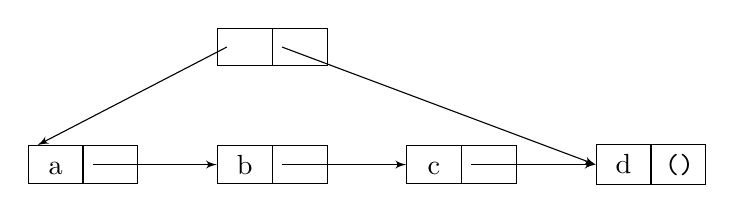
\begin{tikzpicture}[start chain]

\node[list,on chain] (A1) {a \nodepart{two} \phantom{null}};
\node[list,on chain] (A2) {b \nodepart{two} \phantom{null}};
\node[list,on chain] (A3) {c \nodepart{two} \phantom{null}};
\node[list,on chain] (A4) {d \nodepart{two} \texttt{()}};

\node[list,above=of A2] (R) {\phantom{null} \nodepart{two} \phantom{null}};
  
\pSF{A1}{A2};
\pSF{A2}{A3};
\pSF{A3}{A4};

\pFF{R}{A1};
\pSF{R}{A4};

\end{tikzpicture}f
\end{figure}



The last element of the list is a placeholder and not considered part
of the queue.


Four operations on queues are defined below:
\label{start_s182}\texttt{make-queue}, which constructs a queue;
\label{start_s183}\texttt{putq!}, which adds an element to the end
of a queue;
\label{start_s184}\texttt{getq}, which retrieves the element at the
front of a queue; and
\label{start_s185}\texttt{delq!}, which removes the element at the
front of a queue.


\begin{alltt}
(define make-queue
  (lambda ()
    (let ([end (cons 'ignored '())])
      (cons end end))))

(define putq!
  (lambda (q v)
    (let ([end (cons 'ignored '())])
      (set-car! (cdr q) v)
      (set-cdr! (cdr q) end)
      (set-cdr! q end))))

(define getq
  (lambda (q)
    (car (car q))))

(define delq!
  (lambda (q)
    (set-car! q (cdr (car q)))))
\end{alltt}


All are simple operations except for \texttt{putq!}, which modifies the
end pair to contain the new value and adds a new end pair.


\begin{alltt}
(define myq (make-queue))

(putq! myq 'a)
(putq! myq 'b)
(getq myq) \(\Rightarrow\) a
(delq! myq)
(getq myq) \(\Rightarrow\) b
(delq! myq)
(putq! myq 'c)
(putq! myq 'd)
(getq myq) \(\Rightarrow\) c
(delq! myq)
(getq myq) \(\Rightarrow\) d
\end{alltt}

\paragraph{Exercise \label{start_g41}2.9.1}


\label{start_s186}Modify \label{start_s187}\texttt{make-counter} to take two
arguments: an initial value for the
counter to use in place of 0 and an amount to increment the counter
by each time.




\paragraph{Exercise \label{start_g42}2.9.2}


\label{start_s188}Look up the description of \label{start_s189}\texttt{case} in Section \ref{control_g99}.
Replace the \texttt{cond} expression in
\label{start_s190}\texttt{make-stack} with an equivalent
\texttt{case} expression.
Add \texttt{mt?} as a second name for the \texttt{empty?} message.




\paragraph{Exercise \label{start_g43}2.9.3}


\label{start_s191}\label{start_EXSTACKREFANDSET}Modify the \texttt{stack} object to allow the two messages \texttt{ref} and
\texttt{set!}.
\texttt{(\textit{stack} 'ref \textit{i})} should return the \texttt{\textit{i}}th element from
the top of the stack; \texttt{(\textit{stack} 'ref 0)} should be equivalent
to \texttt{(\textit{stack} 'top)}.
\texttt{(\textit{stack} 'set! \textit{i} \textit{v})} should change the \texttt{\textit{i}}th
element from the top of the stack to \texttt{\textit{v}}.


\begin{alltt}
(define stack (make-stack))

(stack 'push! 'a)
(stack 'push! 'b)
(stack 'push! 'c)

(stack 'ref 0) \(\Rightarrow\) c
(stack 'ref 2) \(\Rightarrow\) a
(stack 'set! 1 'd)
(stack 'ref 1) \(\Rightarrow\) d
(stack 'top) \(\Rightarrow\) c
(stack 'pop!)
(stack 'top) \(\Rightarrow\) d
\end{alltt}


[\textit{Hint}: Use \texttt{list-ref} to implement \texttt{ref} and \texttt{list-tail}
with \texttt{set-car!} to implement \texttt{set!}.]




\paragraph{Exercise \label{start_g44}2.9.4}


\label{start_s192}\label{start_s193}Scheme supports \textit{vectors} as well as lists.
Like lists, vectors are aggregate objects that contain other
objects.
Unlike lists, vectors have a fixed size and are laid out
in one flat block of memory, typically with a header containing
the length of the vector, as in the ten-element vector below.


\begin{figure}[H]
\centering
%\includegraphics{math/7.eps}
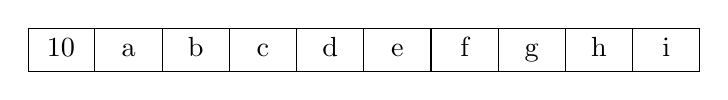
\begin{tikzpicture}
\tikzstyle{bplus}=[
    rectangle split,
    rectangle split horizontal,
    rectangle split ignore empty parts,
    rectangle split part align=base,
    rectangle split parts=10,
    text width=4ex, align=center,
    draw]
\node[bplus] {$10$ \nodepart{two} a \nodepart{three} b \nodepart{four} c \nodepart{five} d \nodepart{six} e \nodepart{seven} f \nodepart{eight} g \nodepart{nine} h \nodepart{ten} i};
\end{tikzpicture}
\end{figure}



This makes vectors more suitable for applications needing
fast access to any element of the aggregate but less suitable for
applications needing data structures that grow and shrink
as needed.


Look up the basic vector operations in
Section \ref{objects_g115} and reimplement the
\texttt{stack} object to use a vector instead of a list to hold
the stack contents.
Include the \texttt{ref} and \texttt{set!} messages of
Exercise \hyperref[start_g43]{2.9.3}.
Have the new \texttt{make-stack} accept a size argument \textit{n}
and make the vector length \textit{n}, but do not otherwise change
the external (abstract) interface.




\paragraph{Exercise \label{start_g45}2.9.5}


\label{start_s194}Define a predicate, \texttt{emptyq?}, for determining if a queue is empty.
Modify \texttt{getq} and \texttt{delq!} to raise an exception when an empty
queue is found, using \texttt{assertion-violation}.




\paragraph{Exercise \label{start_g46}2.9.6}


\label{start_s195}In the queue implementation, the last pair in the encapsulated
list is a placeholder, i.e., it never holds anything useful.
Recode the queue operators to avoid this wasted pair.
Make sure that the series of queue operations given earlier
works with the new implementation.
Which implementation do you prefer?




\paragraph{Exercise \label{start_g47}2.9.7}


\label{start_s196}Using \label{start_s197}\texttt{set-cdr!}, it is possible to create \label{start_s198}\textit{cyclic lists}.
For example, the following expression evaluates to a list whose
car is the symbol \texttt{a} and whose cdr is the list itself.


\begin{alltt}
(let ([ls (cons 'a '())])
  (set-cdr! ls ls)
  ls)
\end{alltt}


What happens when you enter the above expression during an interactive
Scheme session?
What will the implementation of \texttt{length} on page \pageref{start_defn_simplelength}
do when given a cyclic list?
What does the built-in \texttt{length} primitive do?




\paragraph{Exercise \label{start_g48}2.9.8}


\label{start_s199}\label{start_EXLIST_}Define the predicate \label{start_s200}\texttt{list?}, which returns
\texttt{\#{}t} if its argument is a \label{start_s201}proper list and \texttt{\#{}f} otherwise
(see Section \ref{objects_g109}).
It should return \texttt{\#{}f} for cyclic lists as well as for lists
terminated by objects other than \texttt{()}.


\begin{alltt}
(list? '()) \(\Rightarrow\) \#{}t
(list? '(1 2 3)) \(\Rightarrow\) \#{}t
(list? '(a . b)) \(\Rightarrow\) \#{}f
(list? (let ([ls (cons 'a '())])
         (set-cdr! ls ls)
         ls)) \(\Rightarrow\) \#{}f
\end{alltt}


First write a simplified version of \texttt{list?} that does not handle
cyclic lists, then extend this to handle cyclic lists correctly.
Revise your definition until you are satisfied that it is as clear
and concise as possible.
[\textit{Hint}: Use the following "\label{start_s202}hare and tortoise" algorithm to
detect cycles.
Define a recursive help procedure of two arguments, the hare and the tortoise.
Start both the hare and the tortoise at the beginning of the list.
Have the hare advance by two cdrs each time the tortoise
advances by one cdr.
If the hare catches the tortoise, there must be a cycle.]







\chapter{Going Further\label{further_CHPTGOINGFURTHER}}
\label{further_g49}
\label{further_h0}
\begin{figure}[H]
\centering
\setlength{\fboxrule}{3pt}
\fbox{
\includegraphics[width=0.9\textwidth]{canned/ch3.png}
\begin{rotate}{90}
\copyright~2009 Jean-Pierre H\'{e}bert
\end{rotate}}
\end{figure}
\clearpage





The preceding chapter prepared you to write Scheme programs using
a small set of the most useful primitive syntactic forms and
procedures.
This chapter introduces a number of additional features and
programming techniques that will allow you to write more sophisticated
and efficient programs.


\section{\label{further_g50}\label{further_h1}Syntactic Extension\label{further_SECTGFSYNTAX}}



As we saw in Section \ref{start_g21}, the \texttt{let} syntactic form is merely
a \textit{syntactic extension} defined in terms of a \texttt{lambda} expression and
a procedure application, both \label{further_s0}core syntactic forms.
At this point, you might be wondering which \label{further_s1}syntactic forms are core forms
and which are \label{further_s2}syntactic extensions, and how new syntactic extensions
may be defined.  This section provides some answers to these questions.


In truth, it is not necessary for us to draw a distinction between
core forms and syntactic extensions, since once defined, a syntactic
extension has exactly the same status as a core form.
Drawing a distinction, however, makes understanding the language
easier, since it allows us to focus attention on the core forms
and to understand all others in terms of them.


It \textit{is} necessary for a Scheme implementation to distinguish between core
forms and syntactic extensions.
A Scheme implementation \label{further_s3}expands syntactic extensions
into core forms as the first step of compilation or interpretation, allowing
the rest of the compiler or interpreter to focus only on the core forms.
The set of core forms remaining after expansion to be handled directly
by the compiler or interpreter is implementation-dependent, however,
and may be different from the set of forms described as core here.


The exact set of syntactic forms making up the core of the language
is thus subject to debate, although it must be possible to derive
all other forms from any set of forms declared to be core forms.
The set described here is among the simplest for which this constraint
is satisfied.


The core syntactic forms include top-level \texttt{define} forms,
constants, variables, procedure applications,
\label{further_s4}\label{further_s5}\texttt{quote} expressions,
\label{further_s6}\texttt{lambda} expressions,
\label{further_s7}\texttt{if} expressions,
and \label{further_s8}\texttt{set!} expressions.
The grammar below describes the core syntax of Scheme in terms
of these definitions and expressions.
In the grammar, vertical bars ( \textbar{} ) separate alternatives, and a form
followed by an asterisk ( * ) represents zero or more occurrences
of the form.
\textless{}variable\textgreater{} is any Scheme identifier.
\textless{}datum\textgreater{} is any Scheme object, such as a number, list, symbol, or
vector.
\textless{}boolean\textgreater{} is either \texttt{\#{}t} or \texttt{\#{}f},
\textless{}number\textgreater{} is any number,
\textless{}character\textgreater{} is any character, and
\textless{}string\textgreater{} is any string.
We have already seen examples of numbers, strings, lists, symbols, and
booleans.
See Chapter \ref{objects_g106} or the formal syntax description starting on
page \pageref{grammar_APPENDIXFORMALSYNTAX}
for more on the object-level syntax of these
and other objects.


  
  
  {\footnotesize
\begin{tabular}[H]{lcl}

\textless{}program\textgreater{} & \(\longrightarrow\) & \textless{}form\textgreater{}* \\

\textless{}form\textgreater{} & \(\longrightarrow\) & \textless{}definition\textgreater{} \textbar{} \textless{}expression\textgreater{}  \\

\textless{}definition\textgreater{} & \(\longrightarrow\) & \textless{}variable definition\textgreater{} \textbar{} \texttt{(begin} \textless{}definition\textgreater{}*\texttt{)}  \\

\textless{}variable definition\textgreater{} & \(\longrightarrow\) & \texttt{(define} \textless{}variable\textgreater{} \textless{}expression\textgreater{}\texttt{)}  \\

\textless{}expression\textgreater{} & \(\longrightarrow\) & \textless{}constant\textgreater{}  \\

       & \textbar{} & \textless{}variable\textgreater{}  \\

       & \textbar{} & \texttt{(quote} \textless{}datum\textgreater{}\texttt{)}  \\

       & \textbar{} & \texttt{(lambda} \textless{}formals\textgreater{} \textless{}expression\textgreater{} \textless{}expression\textgreater{}*\texttt{)}  \\

       & \textbar{} & \texttt{(if} \textless{}expression\textgreater{} \textless{}expression\textgreater{} \textless{}expression\textgreater{}\texttt{)}  \\

       & \textbar{} & \texttt{(set!} \textless{}variable\textgreater{} \textless{}expression\textgreater{}\texttt{)}  \\

       & \textbar{} & \textless{}application\textgreater{}  \\

\textless{}constant\textgreater{} & \(\longrightarrow\) & \textless{}boolean\textgreater{} \textbar{} \textless{}number\textgreater{} \textbar{} \textless{}character\textgreater{} \textbar{} \textless{}string\textgreater{}  \\

\textless{}formals\textgreater{} & \(\longrightarrow\) & \textless{}variable\textgreater{}  \\

        & \textbar{} & \texttt{(}\textless{}variable\textgreater{}*\texttt{)}  \\

        & \textbar{} & \texttt{(}\textless{}variable\textgreater{} \textless{}variable\textgreater{}* \texttt{.} \textless{}variable\textgreater{}\texttt{)}  \\

\textless{}application\textgreater{} & \(\longrightarrow\) & \texttt{(}\textless{}expression\textgreater{} \textless{}expression\textgreater{}*\texttt{)}
 \\
\end{tabular}
}


The grammar is ambiguous in that the syntax for procedure applications
conflicts with the syntaxes for \texttt{quote}, \texttt{lambda},
\texttt{if}, and \texttt{set!} expressions.
In order to qualify as a procedure application, the first \textless{}expression\textgreater{} must
not be one of these keywords, unless the keyword has been redefined
or locally bound.


The \label{further_s9}``defun'' syntax for \texttt{define} given in
Section \ref{start_g25}
is not included in the core, since definitions in that form are
straightforwardly translated into the simpler \texttt{define} syntax.
Similarly, the core syntax for \texttt{if} does not permit the
\texttt{\textit{alternative}} to be omitted, as did one example in
Section \ref{start_g40}.
An \texttt{if} expression lacking an \texttt{\textit{alternative}} can be translated
into the core syntax for \texttt{if} merely by replacing the missing
subexpression with an arbitrary constant, such as \texttt{\#{}f}.


A \label{further_s10}\texttt{begin} that contains only definitions
is considered to be a
definition in the grammar; this is permitted in order to allow
syntactic extensions to expand into more than one definition.
\texttt{begin} expressions, i.e., \texttt{begin} forms containing expressions,
are not considered core forms.
A \texttt{begin} expression of the form


\texttt{(begin \textit{e\textsubscript{1}} \textit{e\textsubscript{2}} ...)}

is equivalent to the \texttt{lambda} application


\texttt{((lambda () \textit{e\textsubscript{1}} \textit{e\textsubscript{2}} ...))}

and hence need not be considered core.


\label{further_s11}Now that we have established
a set of core syntactic forms, let's turn to a discussion of
\label{further_s12}syntactic extensions.
Syntactic extensions are so called because they extend the syntax of Scheme
beyond the core syntax.
All syntactic extensions in a Scheme program must ultimately
be derived from the core forms.
One syntactic extension, however, may be defined
in terms of another syntactic extension, as long as the latter
is in some sense ``closer'' to the core syntax.
Syntactic forms may appear anywhere an expression or definition is
expected, as long as the extended form expands into a definition or
expression as appropriate.


Syntactic extensions are defined with \label{further_s13}\texttt{define-syntax}.
\texttt{define-syntax} is similar to \texttt{define}, except that \texttt{define-syntax} associates
a syntactic transformation procedure, or \label{further_s14}\textit{transformer}, with
a \label{further_s15}keyword (such as \texttt{let}), rather than associating a value with
a variable.
Here is how we might define \texttt{let} with \texttt{define-syntax}.


\begin{alltt}
(define-syntax let
  (syntax-rules ()
    [(\_{} ((x e) ...) b1 b2 ...)
     ((lambda (x ...) b1 b2 ...) e ...)]))
\end{alltt}


The identifier appearing after \texttt{define-syntax} is the name, or keyword,
of the syntactic extension being defined, in this case \texttt{let}.
The \texttt{syntax-rules} form is an expression that evaluates to a
transformer.
The item following \texttt{syntax-rules} is a list of
\label{further_s16}\textit{auxiliary keywords} and is nearly always \texttt{()}.
An example of an auxiliary keyword is the \texttt{else} of \texttt{cond}.
(Other examples requiring the use of auxiliary keywords are given in
Chapter \ref{syntax_g133}.)
Following the list of auxiliary keywords is a sequence of one or more
\textit{rules}, or \textit{pattern/template} pairs.
Only one rule appears in our definition of \texttt{let}.
The pattern part of a rule specifies the form that the input must take,
and the template specifies to what the input should be transformed.


The pattern should always be a structured expression whose first element
is an \label{further_s17}underscore ( \texttt{\_{}} )\label{further_s18}.
(As we will see in Chapter \ref{syntax_g133}, the use of \texttt{\_{}} is only a
convention, but it is a good one to follow.)
If more than one rule is present, the appropriate one
is chosen by matching the patterns, in order, against the input during
expansion.
It is a syntax violation if none of the patterns match the input.


Identifiers other than an underscore or ellipsis appearing within a
pattern are \label{further_s19}\textit{pattern variables}, unless they
are listed as auxiliary keywords.
Pattern variables match any substructure and are bound to that
substructure within the corresponding template.
\label{further_s20}\label{further_s21}The notation
\texttt{\textit{pat} ...} in the pattern allows for zero or more
expressions matching the ellipsis prototype \texttt{\textit{pat}} in the input.
Similarly, the notation \texttt{\textit{expr} ...} in the template produces
zero or more expressions from the ellipsis prototype \texttt{\textit{expr}} in the output.
The number of \texttt{\textit{pat}}s in the input determines the number of \texttt{\textit{expr}}s
in the output; in order for this to work, any ellipsis prototype in the
template must contain at least one pattern variable from an ellipsis
prototype in the pattern.


The single rule in our definition of \texttt{let} should be fairly
self-explanatory, but a few points are worth mentioning.
First, the syntax of \texttt{let} requires that the body contain at least one
form; hence, we have specified \texttt{b1 b2 ...} instead of
\texttt{b ...}, which might seem more natural.
On the other hand, \texttt{let} does not require that there be at least one
variable/value pair, so we were able to use, simply, \texttt{(x e) ...}.
Second, the pattern variables \texttt{x} and \texttt{e}, though together within
the same prototype in the pattern, are separated in the template; any sort
of rearrangement or recombination is possible.
Finally, the three pattern variables \texttt{x}, \texttt{e}, and \texttt{b2} that
appear in ellipsis prototypes in the pattern also appear in ellipsis
prototypes in the template.
This is not a coincidence; it is a requirement.
In general, if a pattern variable appears within an ellipsis prototype in
the pattern, it cannot appear outside an ellipsis prototype in the template.


The definition of \label{further_s22}\texttt{and} below is somewhat more complex than the
one for \texttt{let}.


\begin{alltt}
(define-syntax and\label{further_defn_and}
  (syntax-rules ()
    [(\_{}) \#{}t]
    [(\_{} e) e]
    [(\_{} e1 e2 e3 ...)
     (if e1 (and e2 e3 ...) \#{}f)]))
\end{alltt}


This definition is recursive and involves more than one rule.
Recall that \texttt{(and)} evaluates to \texttt{\#{}t}; the first rule takes care of
this case.
The second and third rules specify the base case and recursion steps
of the recursion and together translate \texttt{and} expressions with
two or more subexpressions into nested \texttt{if} expressions.
For example, \texttt{(and a b c)} expands first into


\texttt{(if a (and b c) \#{}f)}

then


\texttt{(if a (if b (and c) \#{}f) \#{}f)}

and finally


\texttt{(if a (if b c \#{}f) \#{}f)}

With this expansion, if \texttt{a} and \texttt{b} evaluate to a true value, then the value
is the value of \texttt{c}, otherwise \texttt{\#{}f}, as desired.


The version of \texttt{and} below is simpler but, unfortunately,
incorrect.


\begin{alltt}
(define-syntax and ; incorrect!
  (syntax-rules ()
    [(\_{}) \#{}t]
    [(\_{} e1 e2 ...)
     (if e1 (and e2 ...) \#{}f)]))
\end{alltt}


The expression


\texttt{(and (not (= x 0)) (/ 1 x))}

should return the value of \texttt{(/ 1 x)} when \texttt{x}
is not zero.
With the incorrect version of \texttt{and}, the expression expands
as follows.


\begin{alltt}
(if (not (= x 0)) (and (/ 1 x)) \#{}f) \(\rightarrow\)
  (if (not (= x 0)) (if (/ 1 x) (and) \#{}f) \#{}f) \(\rightarrow\)
  (if (not (= x 0)) (if (/ 1 x) \#{}t \#{}f) \#{}f)
\end{alltt}


The final answer if \texttt{x} is not zero is \texttt{\#{}t}, not the
value of \texttt{(/ 1 x)}.


The definition of \label{further_s23}\texttt{or} below is similar to the one for \texttt{and} except
that a temporary variable must be introduced for each intermediate
value so that we can both test the value and return it if it is a
true value.
(A temporary variable is not needed for \texttt{and} since there is only one
false value, \texttt{\#{}f}.)


\begin{alltt}
(define-syntax or\label{further_defn_or}
  (syntax-rules ()
    [(\_{}) \#{}f]
    [(\_{} e) e]
    [(\_{} e1 e2 e3 ...)
     (let ([t e1])
       (if t t (or e2 e3 ...)))]))
\end{alltt}


Like variables bound by \texttt{lambda} or \texttt{let}, identifiers introduced
by a template are \label{further_s24}lexically scoped, i.e., visible only within
expressions introduced by the template.
Thus, even if one of the expressions \texttt{e2 e3 ...} contains a reference
to \texttt{t}, the introduced binding for \texttt{t} does not ``capture'' those
references.
This is typically accomplished via automatic renaming of introduced
identifiers.


As with the simpler version of \texttt{and} given above, the simpler
version of \texttt{or} below is incorrect.


\begin{alltt}
(define-syntax or ; incorrect!
  (syntax-rules ()
    [(\_{}) \#{}f]
    [(\_{} e1 e2 ...)
     (let ([t e1])
       (if t t (or e2 ...)))]))
\end{alltt}


The reason is more subtle, however, and is the subject of
Exercise \hyperref[further_g61]{3.2.6}.


\paragraph{Exercise \label{further_g51}3.1.1}


\label{further_s25}Write out the expansion steps necessary to expand


\begin{alltt}
(let ([x (memv 'a ls)])
  (and x (memv 'b x)))
\end{alltt}


into core forms.




\paragraph{Exercise \label{further_g52}3.1.2}


\label{further_s26}Write out the expansion steps necessary to expand


\texttt{(or (memv x '(a b c)) (list x))}


into core forms.


\paragraph{Exercise \label{further_g53}3.1.3}


\label{further_s27}\label{further_s28}\texttt{let*} is similar to \texttt{let} but evaluates its bindings
in sequence.
Each of the right-hand-side expressions is within the scope of
the earlier bindings.


\begin{alltt}
(let* ([a 5] [b (+ a a)] [c (+ a b)])
  (list a b c)) \(\Rightarrow\) (5 10 15)
\end{alltt}

\texttt{let*} can be implemented as nested \texttt{let} expressions.
For example, the \texttt{let*} expression above is equivalent to the nested
\texttt{let} expressions below.

\begin{alltt}
(let ([a 5])
  (let ([b (+ a a)])
    (let ([c (+ a b)])
      (list a b c)))) \(\Rightarrow\) (5 10 15)
\end{alltt}


Define \texttt{let*} with \texttt{define-syntax}.




\paragraph{Exercise \label{further_g54}3.1.4}


\label{further_s29}As we saw in Section \ref{start_g40},
it is legal to omit the third, or \textit{alternative}, subexpression
of an \texttt{if} expression.
Doing so, however, often leads to confusion.
Scheme provides two syntactic forms,
\label{further_s30}\texttt{when} and \label{further_s31}\texttt{unless},
that may be used in place of
such ``one-armed'' \texttt{if} expressions.


\begin{alltt}
(when \textit{test} \textit{expr\textsubscript{1}} \textit{expr\textsubscript{2}} ...)
(unless \textit{test} \textit{expr\textsubscript{1}} \textit{expr\textsubscript{2}} ...)
\end{alltt}


With both forms, \texttt{test} is evaluated first.
For \texttt{when}, if \texttt{test} evaluates to true, the remaining
forms are evaluated in sequence as if enclosed in an implicit
\texttt{begin} expression.
If \texttt{test} evaluates to false, the remaining forms are not
evaluated, and the result is unspecified.
\texttt{unless} is similar except that
the remaining forms are evaluated only if \texttt{test}
evaluates to false.


\begin{alltt}
(let ([x 3])
  (unless (= x 0) (set! x (+ x 1)))
  (when (= x 4) (set! x (* x 2)))
  x) \(\Rightarrow\) 8
\end{alltt}


Define \texttt{when} as a syntactic extension in terms of \texttt{if}
and \texttt{begin}, and define \texttt{unless}
in terms of \texttt{when}.




\section{\label{further_g55}\label{further_h2}More Recursion\label{further_SECTGFMORERECURSION}}



\label{further_s32}In Section \ref{start_g32}, we saw how
to define recursive procedures using top-level definitions.
Before that, we saw how to create local bindings for procedures using
\label{further_s33}\texttt{let}.
It is natural to wonder whether a \texttt{let}-bound procedure can be
recursive.
The answer is no, at least not in a straightforward way.
If you try to evaluate the \label{further_s34}expression


\begin{alltt}
(let ([sum (lambda (ls)
             (if (null? ls)
                 0
                 (+ (car ls) (sum (cdr ls)))))])
  (sum '(1 2 3 4 5)))
\end{alltt}


it will probably raise an exception with a message to the effect that \texttt{sum} is
undefined.
This is because the variable \texttt{sum} is visible only within the body
of the \texttt{let} expression and not within the \texttt{lambda} expression
whose value is bound to \texttt{sum}.
We can get around this problem by passing the procedure \texttt{sum} to itself
as follows.


\begin{alltt}
(let ([sum (lambda (sum ls)
             (if (null? ls)
                 0
                 (+ (car ls) (sum sum (cdr ls)))))])
  (sum sum '(1 2 3 4 5))) \(\Rightarrow\) 15
\end{alltt}


This works and is a clever solution, but there is an easier way,
using \label{further_s35}\texttt{letrec}.
Like \texttt{let}, the
\texttt{letrec} syntactic form includes a set of variable-value pairs,
along with a sequence of expressions referred to as the \textit{body} of the
\texttt{letrec}.


\texttt{(letrec ((\textit{var} \textit{expr}) ...) \textit{body\textsubscript{1}} \textit{body\textsubscript{2}} ...)}

Unlike \texttt{let}, the variables \texttt{\textit{var} ...} are visible not
only within the body of the \texttt{letrec} but also within
\texttt{\textit{expr} ...}.
Thus, we can rewrite the expression above as follows.


\begin{alltt}
(letrec ([sum (lambda (ls)
                (if (null? ls)
                    0
                    (+ (car ls) (sum (cdr ls)))))])
  (sum '(1 2 3 4 5))) \(\Rightarrow\) 15
\end{alltt}


Using \texttt{letrec}, we can also define \label{further_s36}mutually recursive procedures, such
as the procedures \label{further_s37}\texttt{even?} and \label{further_s38}\texttt{odd?} that were the subject of
Exercise \hyperref[start_g38]{2.8.6}.


\begin{alltt}
(letrec ([even?\label{further_defn_even__odd_}
          (lambda (x)
            (or (= x 0)
                (odd? (- x 1))))]
         [odd?
          (lambda (x)
            (and (not (= x 0))
                 (even? (- x 1))))])
  (list (even? 20) (odd? 20))) \(\Rightarrow\) (\#{}t \#{}f)
\end{alltt}


In a \texttt{letrec} expression,
\texttt{\textit{expr} ...} are most often \texttt{lambda} expressions,
though this need not be the case.
One restriction on the expressions must be obeyed, however.
It must be possible to evaluate each \texttt{\textit{expr}} without
evaluating any of the variables \texttt{\textit{var} ...}.
This restriction is always satisfied if the expressions are all
\texttt{lambda} expressions, since even though the variables may appear
within the \texttt{lambda} expressions, they cannot be evaluated until
the resulting procedures are invoked in the body of the \texttt{letrec}.
The following \texttt{letrec} expression obeys this restriction.


\begin{alltt}
(letrec ([f (lambda () (+ x 2))]
         [x 1])
  (f)) \(\Rightarrow\) 3
\end{alltt}


while the following does not.


\begin{alltt}
(letrec ([y (+ x 2)]
         [x 1])
  y)
\end{alltt}


In this case, an exception is raised indicating that \texttt{x} is not
defined where it is referenced.


We can use \texttt{letrec} to hide the definitions of ``help'' procedures
so that they do not clutter the top-level namespace.
This is demonstrated by the definition of \label{further_s39}\texttt{list?} below, which
follows the "\label{further_s40}hare and tortoise" algorithm
outlined in Exercise \hyperref[start_g48]{2.9.8}.


\begin{alltt}
(define list?\label{further_defn_list_}
  (lambda (x)
    (letrec ([race
              (lambda (h t)
                (if (pair? h)
                    (let ([h (cdr h)])
                      (if (pair? h)
                          (and (not (eq? h t))
                               (race (cdr h) (cdr t)))
                          (null? h)))
                    (null? h)))])
      (race x x))))
\end{alltt}


When a recursive procedure is called in only one place outside
the procedure, as in the example above, it is often clearer to use
a \label{further_s41}\textit{named} \texttt{let} expression.
Named \texttt{let} expressions take the following form.


\begin{alltt}
(let \textit{name} ((\textit{var} \textit{expr}) ...)
  \textit{body\textsubscript{1}} \textit{body\textsubscript{2}} ...)
\end{alltt}


Named \texttt{let} is similar to unnamed \texttt{let} in that it binds
the variables \texttt{\textit{var} ...} to the values of
\texttt{\textit{expr} ...} within
the body \texttt{\textit{body\textsubscript{1}} \textit{body\textsubscript{2}} ...}.
As with unnamed \texttt{let}, the variables are visible only within the
body and not within \texttt{\textit{expr} ...}.
In addition, the variable \texttt{\textit{name}} is bound within the body to
a procedure that may be called to recur; the arguments to
the procedure become the new values for the variables
\texttt{\textit{var} ...}.


The definition of \label{further_s42}\texttt{list?} has been rewritten below to use named
\texttt{let}.


\begin{alltt}
(define list?
  (lambda (x)
    (let race ([h x] [t x])
      (if (pair? h)
          (let ([h (cdr h)])
            (if (pair? h)
                (and (not (eq? h t))
                     (race (cdr h) (cdr t)))
                (null? h)))
          (null? h)))))
\end{alltt}


Just as \texttt{let} can be expressed as a simple direct application
of a \texttt{lambda} expression to arguments, named \texttt{let} can be expressed
as the application of a recursive procedure to arguments.
A named \texttt{let} of the form


\begin{alltt}
(let \textit{name} ((\textit{var} \textit{expr}) ...)
  \textit{body\textsubscript{1}} \textit{body\textsubscript{2}} ...)
\end{alltt}


can be rewritten in terms of \texttt{letrec} as follows.


\begin{alltt}
((letrec ((\textit{name} (lambda (\textit{var} ...) \textit{body\textsubscript{1}} \textit{body\textsubscript{2}} ...)))
   \textit{name})
 \textit{expr} ...)
\end{alltt}


Alternatively, it can be rewritten as


\begin{alltt}
(letrec ((\textit{name} (lambda (\textit{var} ...) \textit{body\textsubscript{1}} \textit{body\textsubscript{2}} ...)))
  (\textit{name} \textit{expr} ...))
\end{alltt}


provided that the variable \texttt{\textit{name}} does not appear free within
\texttt{\textit{expr} ...}.


As we discussed in Section \ref{start_g32}, some recursion is
essentially \label{further_s43}iteration and executes as such.
When a procedure call is in tail position (see below) with respect to
a \texttt{lambda}
expression, it is considered to be a \label{further_s44}\textit{tail call}, and
Scheme systems must treat it \textit{properly}, as a ``goto''
or jump.
When a procedure tail-calls itself or calls itself indirectly
through a series of tail calls, the result is \label{further_s45}\textit{tail recursion}.
Because tail calls are treated as jumps, tail recursion can be used
for indefinite iteration in place of the more restrictive iteration
constructs provided by other programming languages, without fear of
overflowing any sort of recursion stack.


A call is in tail position with respect to a \texttt{lambda} expression
if its value is returned directly from the \texttt{lambda} expression,
i.e., if nothing is left to do after the call but to return from the
\texttt{lambda} expression.
For example, a call is in tail position if
it is the last expression in the body of a \texttt{lambda} expression,
the \textit{consequent} or \textit{alternative} part of an \texttt{if} expression
in tail position,
the last subexpression of an \texttt{and} or \texttt{or} expression in tail
position,
the last expression in the body of a \texttt{let} or \texttt{letrec}
in tail position, etc.
Each of the calls to \texttt{f} in the expressions below
are tail calls, but the calls to \texttt{g} are not.


\begin{alltt}
(lambda () (f (g)))
(lambda () (if (g) (f) (f)))
(lambda () (let ([x 4]) (f)))
(lambda () (or (g) (f)))
\end{alltt}


In each case, the values of the calls to \texttt{f} are returned directly,
whereas the calls to \texttt{g} are not.


Recursion in general and named \texttt{let} in particular provide a natural
way to implement many algorithms, whether iterative, recursive, or
partly iterative and partly recursive; the programmer is not burdened
with two distinct mechanisms.


The following two definitions of \label{further_s46}\texttt{factorial} use named \texttt{let}
expressions to compute the factorial, \textit{n}!, of a nonnegative integer \textit{n}.
The first employs the recursive definition \textit{n}! = \textit{n} \(\times\) (\textit{n} - 1)!,
where 0! is defined to be 1.


\begin{alltt}
(define factorial
  (lambda (n)
    (let fact ([i n])
      (if (= i 0)
          1
          (* i (fact (- i 1)))))))
\end{alltt}


\begin{alltt}
(factorial 0) \(\Rightarrow\) 1
(factorial 1) \(\Rightarrow\) 1
(factorial 2) \(\Rightarrow\) 2
(factorial 3) \(\Rightarrow\) 6
(factorial 10) \(\Rightarrow\) 3628800
\end{alltt}


The second is an iterative version that employs the iterative definition
\textit{n}! = \textit{n} \(\times\) (\textit{n} - 1) \(\times\) (\textit{n} - 2) \(\times\) ... \(\times\) 1, using an accumulator,
\texttt{a}, to hold the intermediate products.


\begin{alltt}
(define factorial
  (lambda (n)
    (let fact ([i n] [a 1])
      (if (= i 0)
          a
          (fact (- i 1) (* a i))))))
\end{alltt}


\label{further_fibonacci}A similar problem is to compute the \textit{n}th Fibonacci number for a given
\textit{n}.
\label{further_s47}The \label{further_s48}\textit{Fibonacci numbers} are an infinite sequence of
integers, 0, 1, 1, 2, 3, 5, 8, etc., in which each
number is the sum of the two preceding numbers in the sequence.
A procedure to compute the \textit{n}th Fibonacci number is most naturally
defined recursively as follows.


\begin{alltt}
(define fibonacci
  (lambda (n)
    (let fib ([i n])
      (cond
        [(= i 0) 0]
        [(= i 1) 1]
        [else (+ (fib (- i 1)) (fib (- i 2)))]))))

(fibonacci 0) \(\Rightarrow\) 0
(fibonacci 1) \(\Rightarrow\) 1
(fibonacci 2) \(\Rightarrow\) 1
(fibonacci 3) \(\Rightarrow\) 2
(fibonacci 4) \(\Rightarrow\) 3
(fibonacci 5) \(\Rightarrow\) 5
(fibonacci 6) \(\Rightarrow\) 8
(fibonacci 20) \(\Rightarrow\) 6765
(fibonacci 30) \(\Rightarrow\) 832040
\end{alltt}


This solution requires the computation of the two preceding Fibonacci
numbers at each step and hence is \label{further_s49}\textit{doubly recursive}.
For example, to compute \texttt{(fibonacci 4)} requires the computation of both
\texttt{(fib 3)} and \texttt{(fib 2)}, to compute \texttt{(fib 3)} requires computing
both \texttt{(fib 2)} and \texttt{(fib 1)}, and to compute \texttt{(fib 2)} requires
computing both \texttt{(fib 1)} and \texttt{(fib 0)}.
This is very inefficient, and it becomes more inefficient as \texttt{n} grows.
A more efficient solution is to adapt the accumulator solution of the
\texttt{factorial} example above to use two accumulators, \texttt{a1} for the
current Fibonacci number and \texttt{a2} for the preceding one.


\begin{alltt}
(define fibonacci
  (lambda (n)
    (if (= n 0)
        0
        (let fib ([i n] [a1 1] [a2 0])
          (if (= i 1)
              a1
              (fib (- i 1) (+ a1 a2) a1))))))
\end{alltt}


Here, zero is treated as a special case, since there is no preceding value.
This allows us to use the single base case \texttt{(= i 1)}.
The time it takes to compute the \textit{n}th Fibonacci number using this
iterative solution grows linearly with \textit{n}, which makes a
significant difference when compared to the doubly recursive version.
To get a feel for the difference, try computing \texttt{(fibonacci 35)} and
\texttt{(fibonacci 40)} using
both definitions to see how long each takes.


We can also get a feel for the difference by looking at a trace for
each on small inputs.
The first trace below shows the calls to \texttt{fib} in the non-tail-recursive
version of \texttt{fibonacci}, with input 5.


\begin{alltt}
\textbar{}(fib 5)
\textbar{} (fib 4)
\textbar{} \textbar{}(fib 3)
\textbar{} \textbar{} (fib 2)
\textbar{} \textbar{} \textbar{}(fib 1)
\textbar{} \textbar{} \textbar{}1
\textbar{} \textbar{} \textbar{}(fib 0)
\textbar{} \textbar{} \textbar{}0
\textbar{} \textbar{} 1
\textbar{} \textbar{} (fib 1)
\textbar{} \textbar{} 1
\textbar{} \textbar{}2
\textbar{} \textbar{}(fib 2)
\textbar{} \textbar{} (fib 1)
\textbar{} \textbar{} 1
\textbar{} \textbar{} (fib 0)
\textbar{} \textbar{} 0
\textbar{} \textbar{}1
\textbar{} 3
\textbar{} (fib 3)
\textbar{} \textbar{}(fib 2)
\textbar{} \textbar{} (fib 1)
\textbar{} \textbar{} 1
\textbar{} \textbar{} (fib 0)
\textbar{} \textbar{} 0
\textbar{} \textbar{}1
\textbar{} \textbar{}(fib 1)
\textbar{} \textbar{}1
\textbar{} 2
\textbar{}5
\end{alltt}


Notice how there are several calls to \texttt{fib} with arguments 2, 1, and 0.
The second trace shows the calls to \texttt{fib} in the tail-recursive version,
again with input 5.


\begin{alltt}
\textbar{}(fib 5 1 0)
\textbar{}(fib 4 1 1)
\textbar{}(fib 3 2 1)
\textbar{}(fib 2 3 2)
\textbar{}(fib 1 5 3)
\textbar{}5
\end{alltt}


Clearly, there is quite a difference.


The \label{further_s50}named \texttt{let} examples shown so far are either tail-recursive or not
tail-recursive.
It often happens that one recursive call within the same expression is
tail-recursive while another is not.
The definition of \label{further_s51}\texttt{factor} below computes the prime factors of its
nonnegative integer argument.
The first call to \texttt{f} is not
tail-recursive, but the second one is.


\begin{alltt}
(define factor
  (lambda (n)
    (let f ([n n] [i 2])
      (cond
        [(\textgreater{}= i n) (list n)]
        [(integer? (/ n i))
         (cons i (f (/ n i) i))]
        [else (f n (+ i 1))]))))

(factor 0) \(\Rightarrow\) (0)
(factor 1) \(\Rightarrow\) (1)
(factor 12) \(\Rightarrow\) (2 2 3)
(factor 3628800) \(\Rightarrow\) (2 2 2 2 2 2 2 2 3 3 3 3 5 5 7)
(factor 9239) \(\Rightarrow\) (9239)
\end{alltt}


A trace of the calls to \texttt{f}, produced in Chez Scheme by
replacing \texttt{let} with \texttt{trace-let},
in the evaluation of \texttt{(factor 120)}
below highlights the difference between the nontail calls and the
tail calls.


\begin{alltt}
\textbar{}(f 120 2)
\textbar{} (f 60 2)
\textbar{} \textbar{}(f 30 2)
\textbar{} \textbar{} (f 15 2)
\textbar{} \textbar{} (f 15 3)
\textbar{} \textbar{} \textbar{}(f 5 3)
\textbar{} \textbar{} \textbar{}(f 5 4)
\textbar{} \textbar{} \textbar{}(f 5 5)
\textbar{} \textbar{} \textbar{}(5)
\textbar{} \textbar{} (3 5)
\textbar{} \textbar{}(2 3 5)
\textbar{} (2 2 3 5)
\textbar{}(2 2 2 3 5)
\end{alltt}


A nontail call to \texttt{f} is shown indented relative to its caller,
since the caller is still active, whereas tail calls appear at
the same level of indentation.


\paragraph{Exercise \label{further_g56}3.2.1}


\label{further_s52}Which of the recursive procedures defined in Section \ref{further_g55} are
tail-recursive, and which are not?




\paragraph{Exercise \label{further_g57}3.2.2}


\label{further_s53}Rewrite \label{further_s54}\texttt{factor} using \texttt{letrec} to bind \texttt{f} in place of named \texttt{let}.
Which version do you prefer?




\paragraph{Exercise \label{further_g58}3.2.3}


\label{further_s55}Can the \texttt{letrec} expression below
be rewritten using named \texttt{let}?
If not, why not?
If so, do it.


\begin{alltt}
(letrec ([even?
          (lambda (x)
            (or (= x 0)
                (odd? (- x 1))))]
         [odd?
          (lambda (x)
            (and (not (= x 0))
                 (even? (- x 1))))])
  (even? 20))
\end{alltt}



\paragraph{Exercise \label{further_g59}3.2.4}


\label{further_s56}Rewrite both definitions of \texttt{fibonacci} given in this section to count
the number of recursive calls to \texttt{fib}, using a counter similar to the
one used in the \texttt{cons-count} example of Section \ref{start_g40}.
Count the number of recursive calls made in each case for several
input values.
What do you notice?




\paragraph{Exercise \label{further_g60}3.2.5}


\label{further_s57}Augment the definition of \texttt{let} given in Section \ref{further_g50} to
handle named \texttt{let} as well as unnamed \texttt{let}, using two rules.




\paragraph{Exercise \label{further_g61}3.2.6}


\label{further_s58}\label{further_ex_incorrect_or}The following definition of \texttt{or} is simpler than the one given
in Section \ref{further_g50}.


\begin{alltt}
(define-syntax or ; incorrect!
  (syntax-rules ()
    [(\_{}) \#{}f]
    [(\_{} e1 e2 ...)
     (let ([t e1])
       (if t t (or e2 ...)))]))
\end{alltt}


Say why it is not correct.
[\textit{Hint}: Think about what would happen if this version of \texttt{or}
were used in the \texttt{even?} and \texttt{odd?} example given
on page \pageref{further_defn_even__odd_} for very large inputs.]




\paragraph{Exercise \label{further_g62}3.2.7}


\label{further_s59}The definition of \label{further_s60}\texttt{factor} is not the most efficient possible.
First, no factors of \textit{n} besides \textit{n} itself can possibly be found
beyond \(\sqrt{n}\).
Second, the division \texttt{(/ n i)} is performed twice when a factor is
found.
Third, after 2, no even factors can possibly be found.
Recode \texttt{factor} to correct all three problems.
Which is the most important problem to solve?
Are there any additional improvements you can make?




\section{\label{further_g63}\label{further_h3}Continuations\label{further_SECTGFCONTINUATIONS}}



\label{further_s61}During the evaluation of a Scheme expression, the
implementation must keep track of two things:
(1) what to evaluate and (2) what to do with the value.
Consider the evaluation of \texttt{(null? x)} within the expression
below.


\texttt{(if (null? x) (quote ()) (cdr x))}

The implementation must first evaluate \texttt{(null? x)} and, based on its value,
evaluate either \texttt{(quote ())} or \texttt{(cdr x)}.
``What to evaluate'' is \texttt{(null? x)}, and ``what to do with the value''
is to make the decision which of \texttt{(quote ())} and \texttt{(cdr x)} to
evaluate and to do so.
We call ``what to do with the value'' the \textit{continuation} of a
computation.


Thus, at any point during the evaluation of any expression, there is a
continuation ready to complete, or at least \textit{continue}, the computation
from that point.
Let's assume that \texttt{x} has the value \texttt{(a b c)}.
We can isolate six continuations during the evaluation of
\texttt{(if (null? x) (quote ()) (cdr x))}, the continuations waiting for

\begin{enumerate}
\label{further_g64}\item 
the value of \texttt{(if (null? x) (quote ()) (cdr x))},
\label{further_g65}\item the value of \texttt{(null? x)},
\label{further_g66}\item the value of \texttt{null?},
\label{further_g67}\item the value of \texttt{x},
\label{further_g68}\item the value of \texttt{cdr}, and
\label{further_g69}\item the value of \texttt{x} (again).

\end{enumerate}


The continuation of \texttt{(cdr x)} is not listed because it is the same
as the one waiting for \texttt{(if (null? x) (quote ()) (cdr x))}.


Scheme allows the continuation of any expression to be captured with
the procedure
\label{further_s62}\texttt{call/cc}.
\texttt{call/cc} must be passed a procedure \texttt{\textit{p}} of
one argument.
\texttt{call/cc} constructs a concrete representation of the
current continuation and passes it to \texttt{\textit{p}}.
The continuation itself is represented by a procedure \texttt{\textit{k}}.
Each time \texttt{\textit{k}} is applied to a value, it returns
the value to the continuation of the \texttt{call/cc} application.
This value becomes, in essence, the value of the application of
\texttt{call/cc}.


If \texttt{\textit{p}} returns without invoking \texttt{\textit{k}},
the value returned by the procedure becomes the value of the
application of \texttt{call/cc}.


Consider the simple examples below.


\begin{alltt}
(call/cc
  (lambda (k)
    (* 5 4))) \(\Rightarrow\) 20

(call/cc
  (lambda (k)
    (* 5 (k 4)))) \(\Rightarrow\) 4

(+ 2
   (call/cc
     (lambda (k)
       (* 5 (k 4))))) \(\Rightarrow\) 6
\end{alltt}


In the first example, the continuation is captured and bound to \texttt{k},
but \texttt{k} is never used, so the value is simply the product
of 5 and 4.
In the second, the continuation is invoked before the multiplication, so
the value is the value passed to the continuation, 4.
In the third, the continuation includes the addition by 2; thus, the
value is the value passed to the continuation, 4, plus 2.


\label{further_s63}Here is a less trivial example, showing the use of
\texttt{call/cc} to provide a nonlocal exit from a recursion.


\begin{alltt}
(define product\label{further_defn_product_call_cc}
  (lambda (ls)
    (call/cc
      (lambda (break)
        (let f ([ls ls])
          (cond
            [(null? ls) 1]
            [(= (car ls) 0) (break 0)]
            [else (* (car ls) (f (cdr ls)))]))))))
\end{alltt}


\begin{alltt}
(product '(1 2 3 4 5)) \(\Rightarrow\) 120
(product '(7 3 8 0 1 9 5)) \(\Rightarrow\) 0
\end{alltt}


The nonlocal exit allows \texttt{product} to return immediately,
without performing the pending multiplications,
when a zero value is detected.


Each of the continuation invocations above returns to the continuation
while control remains within the procedure passed to \texttt{call/cc}.
The following example uses the continuation after this procedure
has already returned.


\begin{alltt}
(let ([x (call/cc (lambda (k) k))])
  (x (lambda (ignore) "hi"))) \(\Rightarrow\) "hi"
\end{alltt}


The continuation captured by this invocation of \texttt{call/cc} may be described as
"Take the value, bind it to \texttt{x}, and apply the value of \texttt{x} to
the value of \texttt{(lambda (ignore) "hi")}."
Since \texttt{(lambda (k) k)} returns its argument, \texttt{x} is bound to the
continuation itself; this continuation is applied to the procedure resulting
from the evaluation of \texttt{(lambda (ignore) "hi")}.
This has the effect of binding \texttt{x} (again!) to this procedure and
applying the procedure to itself.
The procedure ignores its argument and returns \texttt{"hi"}.


The following variation of the example above is probably the most confusing
Scheme program of its size; it might be easy to guess what it returns,
but it takes some thought to figure out why.


\texttt{(((call/cc (lambda (k) k)) (lambda (x) x)) "HEY!") \(\Rightarrow\) "HEY!"}

The value of the \texttt{call/cc} is its own continuation, as in the preceding
example.
This is applied to the identity procedure \texttt{(lambda (x) x)}, so the
\texttt{call/cc} returns a second time with this value.
Then, the identity procedure is applied to itself, yielding the identity
procedure.
This is finally applied to \texttt{"HEY!"}, yielding \texttt{"HEY!"}.


Continuations used in this manner are not always so puzzling.
Consider the following definition of \label{further_s64}\texttt{factorial} that saves the
continuation at the base of the recursion before returning 1, by
assigning the top-level variable \label{further_s65}\texttt{retry}\label{further_retry}.


\begin{alltt}
(define retry \#{}f)

(define factorial
  (lambda (x)
    (if (= x 0)
        (call/cc (lambda (k) (set! retry k) 1))
        (* x (factorial (- x 1))))))
\end{alltt}


With this definition, \texttt{factorial} works as we expect
\texttt{factorial} to work, except it has the side effect of assigning
\texttt{retry}.


\begin{alltt}
(factorial 4) \(\Rightarrow\) 24
(retry 1) \(\Rightarrow\) 24
(retry 2) \(\Rightarrow\) 48
\end{alltt}


The continuation bound to \texttt{retry} might be described as "Multiply
the value by 1, then multiply this result by 2, then multiply
this result by 3, then multiply this result by 4."
If we pass the continuation a different value, i.e., not 1, we will
cause the base value to be something other than 1 and hence change
the end result.


\begin{alltt}
(retry 2) \(\Rightarrow\) 48
(retry 5) \(\Rightarrow\) 120
\end{alltt}


This mechanism could be the basis for a breakpoint package implemented with
\texttt{call/cc}; each time a breakpoint is encountered, the continuation of
the breakpoint is saved so that the computation may be restarted from the
breakpoint (more than once, if desired).


Continuations may be used to implement various forms of multitasking.
The simple ``light-weight process'' mechanism defined below allows
multiple computations to be interleaved.
Since it is \textit{nonpreemptive}, it requires that each process voluntarily
``pause'' from time to time in order to allow the others to run.


\begin{alltt}
(define lwp-list '())
(define lwp
  (lambda (thunk)
    (set! lwp-list (append lwp-list (list thunk)))))

(define start
  (lambda ()
    (let ([p (car lwp-list)])
      (set! lwp-list (cdr lwp-list))
      (p))))
\end{alltt}


\begin{alltt}
(define pause
  (lambda ()
    (call/cc
      (lambda (k)
        (lwp (lambda () (k \#{}f)))
        (start)))))
\end{alltt}


The following light-weight processes cooperate to print an
infinite sequence of lines containing \texttt{"hey!"}.


\begin{alltt}
(lwp (lambda () (let f () (pause) (display "h") (f))))
(lwp (lambda () (let f () (pause) (display "e") (f))))
(lwp (lambda () (let f () (pause) (display "y") (f))))
(lwp (lambda () (let f () (pause) (display "!") (f))))
(lwp (lambda () (let f () (pause) (newline) (f))))
(start) \(\Rightarrow\) \textit{hey!}
         \textit{hey!}
         \textit{hey!}
         \textit{hey!}
         \(\vdots\)
\end{alltt}


See Section \ref{examples_g208} for an implementation of \textit{engines},
which support preemptive multitasking, with \texttt{call/cc}.


\paragraph{Exercise \label{further_g70}3.3.1}


\label{further_s66}Use \texttt{call/cc} to write a program that loops indefinitely, printing
a sequence of numbers beginning at zero.
Do not use any recursive procedures, and do not use any assignments.




\paragraph{Exercise \label{further_g71}3.3.2}


\label{further_s67}Rewrite \texttt{product} without \texttt{call/cc}, retaining the feature that no
multiplications are performed if any of the list elements are zero.




\paragraph{Exercise \label{further_g72}3.3.3}


\label{further_s68}What would happen if a process created by \texttt{lwp} as defined above
were to terminate, i.e., simply return without calling
\texttt{pause}?
Define a \texttt{quit} procedure that allows a process to terminate
without otherwise affecting the \texttt{lwp} system.
Be sure to handle the case in which the only remaining process
terminates.




\paragraph{Exercise \label{further_g73}3.3.4}


\label{further_s69}Each time \texttt{lwp} is called, the list of processes is copied
because \texttt{lwp} uses \texttt{append} to add its argument to the
end of the process list.
Modify the original \texttt{lwp} code to
use the queue data type developed in Section \ref{start_g40}
to avoid this problem.




\paragraph{Exercise \label{further_g74}3.3.5}


\label{further_s70}The light-weight process mechanism allows new processes to be created
dynamically, although the example given in this section does not
do so.
Design an application that requires new processes to be created
dynamically and implement it using the light-weight process mechanism.



\section{\label{further_g75}\label{further_h4}Continuation Passing Style\label{further_SECTGFCPS}}



\label{further_s71}\label{further_s72}As we discussed in the
preceding section, a continuation
waits for the value of each expression.
In particular, a continuation is associated with each procedure call.
When one procedure invokes another via a nontail call, the called
procedure receives an implicit continuation that is responsible for
completing what is left of the calling procedure's body plus returning
to the calling procedure's continuation.
If the call is a tail call, the called procedure simply receives
the continuation of the calling procedure.


We can make the continuations explicit by encapsulating ``what to do''
in an explicit procedural argument passed along on each call.
For example, the continuation of the call to \texttt{f} in


\begin{alltt}
(letrec ([f (lambda (x) (cons 'a x))]
         [g (lambda (x) (cons 'b (f x)))]
         [h (lambda (x) (g (cons 'c x)))])
  (cons 'd (h '()))) \(\Rightarrow\) (d b a c)
\end{alltt}


conses the symbol \texttt{b} onto the value returned to it, then returns
the result of this cons to the continuation of the call to \texttt{g}.
This continuation is the same as the continuation of the call to
\texttt{h}, which conses the symbol \texttt{d} onto the value returned to
it.
We can rewrite this in \textit{continuation-passing style}, or CPS,
by replacing these implicit continuations with explicit procedures.


\begin{alltt}
(letrec ([f (lambda (x k) (k (cons 'a x)))]
         [g (lambda (x k)
              (f x (lambda (v) (k (cons 'b v)))))]
         [h (lambda (x k) (g (cons 'c x) k))])
  (h '() (lambda (v) (cons 'd v))))
\end{alltt}


Like the implicit continuation of \texttt{h} and \texttt{g} in the preceding
example, the explicit continuation passed to \texttt{h} and on to \texttt{g},


\texttt{(lambda (v) (cons 'd v))}

conses the symbol \texttt{d} onto the value passed to it.
Similarly,
the continuation passed to \texttt{f},


\texttt{(lambda (v) (k (cons 'b v)))}

conses \texttt{b} onto the value passed to it, then passes this on to the
continuation of \texttt{g}.


Expressions written in CPS are more complicated, of course, but
this style of programming has some useful applications.
CPS allows
a procedure to pass more than one result to its continuation,
because the procedure that implements the continuation can
take any number of arguments.


\begin{alltt}
(define car\&{}cdr
  (lambda (p k)
    (k (car p) (cdr p))))

(car\&{}cdr '(a b c)
  (lambda (x y)
    (list y x))) \(\Rightarrow\) ((b c) a)
(car\&{}cdr '(a b c) cons) \(\Rightarrow\) (a b c)
(car\&{}cdr '(a b c a d) memv) \(\Rightarrow\) (a d)
\end{alltt}


(This can be done with multiple values as well; see Section \ref{control_g104}.)
CPS also allows a procedure to take separate ``success'' and
``failure'' continuations, which may accept different numbers of arguments.
An example is \label{further_s73}\texttt{integer-divide} below, which passes the quotient
and remainder of its first two arguments to its third, unless the
second argument (the divisor) is zero, in which case it passes an
error message to its fourth argument.


\begin{alltt}
(define integer-divide
  (lambda (x y success failure)
    (if (= y 0)
        (failure "divide by zero")
        (let ([q (quotient x y)])
          (success q (- x (* q y)))))))

(integer-divide 10 3 list (lambda (x) x)) \(\Rightarrow\) (3 1)
(integer-divide 10 0 list (lambda (x) x)) \(\Rightarrow\) "divide by zero"
\end{alltt}


The procedure \texttt{quotient}, employed by \texttt{integer-divide},
returns the quotient of its two arguments,
truncated toward zero.


Explicit success and failure continuations can sometimes
help to avoid the extra communication necessary to separate successful
execution of a procedure from unsuccessful execution.
Furthermore, it is possible to have multiple success or failure
continuations for different flavors of success or failure, each
possibly taking different numbers and types of arguments.
See Sections \ref{examples_g204} and \ref{examples_g208} for extended examples
that employ continuation-passing style.


At this point you might be wondering about the relationship between
CPS and the continuations captured via \texttt{call/cc}.
It turns out that any program that uses \texttt{call/cc} can be rewritten
in CPS without \texttt{call/cc}, but a total rewrite of the program
(sometimes including even system-defined primitives) might be
necessary.
Try to convert the \label{further_s74}\texttt{product} example on
page \pageref{further_defn_product_call_cc}
into CPS before looking at the version below.


\begin{alltt}
(define product
  (lambda (ls k)
    (let ([break k])
      (let f ([ls ls] [k k])
        (cond
          [(null? ls) (k 1)]
          [(= (car ls) 0) (break 0)]
          [else (f (cdr ls)
                   (lambda (x)
                     (k (* (car ls) x))))])))))
\end{alltt}


\begin{alltt}
(product '(1 2 3 4 5) (lambda (x) x)) \(\Rightarrow\) 120
(product '(7 3 8 0 1 9 5) (lambda (x) x)) \(\Rightarrow\) 0
\end{alltt}

\paragraph{Exercise \label{further_g76}3.4.1}


\label{further_s75}Rewrite the \label{further_s76}\texttt{reciprocal} example first given in
Section \ref{start_g5} to accept both success and failure
continuations, like \texttt{integer-divide} above.




\paragraph{Exercise \label{further_g77}3.4.2}


\label{further_s77}Rewrite the \label{further_s78}\texttt{retry} example from page \pageref{further_retry} to use CPS.




\paragraph{Exercise \label{further_g78}3.4.3}


\label{further_s79}Rewrite the following expression in CPS to avoid using \texttt{call/cc}.


\begin{alltt}
(define reciprocals
  (lambda (ls)
    (call/cc
      (lambda (k)
        (map (lambda (x)
               (if (= x 0)
                   (k "zero found")
                   (/ 1 x)))
             ls)))))
\end{alltt}


\begin{alltt}
(reciprocals '(2 1/3 5 1/4)) \(\Rightarrow\) (1/2 3 1/5 4)
(reciprocals '(2 1/3 0 5 1/4)) \(\Rightarrow\) "zero found"
\end{alltt}


[\textit{Hint}: A single-list version of \texttt{map} is
defined on page \pageref{start_defn_map1}.]




\section{\label{further_g79}\label{further_h5}Internal Definitions\label{further_SECTGFINTERNAL}}



\label{further_s80}\label{further_s81}In Section \ref{start_g25}, we
discussed top-level definitions.
Definitions may also appear at the front of a \texttt{lambda}, \texttt{let},
or \texttt{letrec} body, in which case the bindings they create are local
to the body.


\begin{alltt}
(define f (lambda (x) (* x x)))
(let ([x 3])
  (define f (lambda (y) (+ y x)))
  (f 4)) \(\Rightarrow\) 7
(f 4) \(\Rightarrow\) 16
\end{alltt}


Procedures bound by internal definitions can be mutually recursive,
as with \texttt{letrec}.
For example, we can rewrite the \label{further_s82}\texttt{even?} and \label{further_s83}\texttt{odd?} example
from Section \ref{further_g55}
using internal definitions as follows.


\begin{alltt}
(let ()
  (define even?
    (lambda (x)
      (or (= x 0)
          (odd? (- x 1)))))
  (define odd?
    (lambda (x)
      (and (not (= x 0))
           (even? (- x 1)))))
  (even? 20)) \(\Rightarrow\) \#{}t
\end{alltt}


Similarly, we can replace the use of \label{further_s84}\texttt{letrec} to bind \texttt{race}
with an internal definition of \texttt{race} in our first definition of
\label{further_s85}\texttt{list?}.


\begin{alltt}
(define list?
  (lambda (x)
    (define race
      (lambda (h t)
        (if (pair? h)
            (let ([h (cdr h)])
              (if (pair? h)
                  (and (not (eq? h t))
                       (race (cdr h) (cdr t)))
                  (null? h)))
            (null? h))))
    (race x x)))
\end{alltt}


In fact, internal variable definitions and \texttt{letrec} are practically interchangeable.
The only difference, other than the obvious difference in syntax, is that
variable definitions are guaranteed to be evaluated from left to right,
while the bindings of a letrec may be evaluated in any order.
So we cannot quite replace a
\texttt{lambda}, \texttt{let}, or
\texttt{letrec} body containing internal definitions with a \texttt{letrec} expression.
We can, however, use \texttt{letrec*}, which, like
\texttt{let*}, guarantees left-to-right evaluation order.
A body of the form


\begin{alltt}
(define \textit{var} \textit{expr\textsubscript{0}})
  \(\vdots\)
\textit{expr\textsubscript{1}}
\textit{expr\textsubscript{2}}
  \(\vdots\)
\end{alltt}


is equivalent to a \texttt{letrec*}
expression binding the defined variables to the associated values
in a body comprising the expressions.


\texttt{(letrec* ((\textit{var} \textit{expr\textsubscript{0}}) ...) \textit{expr\textsubscript{1}} \textit{expr\textsubscript{2}} ...)}

Conversely, a \texttt{letrec*} of the form


\texttt{(letrec* ((\textit{var} \textit{expr\textsubscript{0}}) ...) \textit{expr\textsubscript{1}} \textit{expr\textsubscript{2}} ...)}

can be replaced with a \texttt{let} expression containing internal definitions
and the expressions from the body as follows.


\begin{alltt}
(let ()
  (define \textit{var} \textit{expr\textsubscript{0}})
    \(\vdots\)
  \textit{expr\textsubscript{1}}
  \textit{expr\textsubscript{2}}
    \(\vdots\)
)
\end{alltt}


The seeming lack of symmetry between these transformations is due to
the fact that \texttt{letrec*} expressions can appear anywhere an expression
is valid, whereas internal definitions can appear only at the front
of a body.
Thus, in replacing a \texttt{letrec*} with internal definitions, we must generally
introduce a \texttt{let} expression to hold the definitions.


Another difference between internal definitions and \texttt{letrec} or
\texttt{letrec*} is that syntax definitions may appear among the internal
definitions, while \texttt{letrec} and \texttt{letrec*} bind only
variables.


\begin{alltt}
(let ([x 3])
  (define-syntax set-x!
    (syntax-rules ()
      [(\_{} e) (set! x e)]))
  (set-x! (+ x x))
  x) \(\Rightarrow\) 6
\end{alltt}


The scope of a syntactic extension established by an internal syntax
definition, as with an internal variable definition, is limited to
the body in which the syntax definition appears.


Internal definitions may be used in conjunction with top-level
definitions and assignments to help modularize programs.
Each module of a program should make visible only those bindings
that are needed by other modules, while hiding other bindings that
would otherwise clutter the top-level namespace and possibly
result in unintended use or redefinition of those bindings.
A common way of structuring a module is shown below.


\begin{alltt}
(define \textit{export-var} \#{}f)
  \(\vdots\)
(let ()
  (define \textit{var} \textit{expr})
    \(\vdots\)
  \textit{init-expr}
    \(\vdots\)
  (set! \textit{export-var} \textit{export-val})
    \(\vdots\)
)
\end{alltt}


The first set of definitions establish top-level bindings for the
variables we desire to export (make visible globally).
The second set of definitions establish local bindings visible only
within the module.
The expressions \texttt{\textit{init-expr} ...} perform any initialization that
must occur after the local bindings have been established.
Finally, the \texttt{set!} expressions assign the exported variables to
the appropriate values.


An advantage of this form of modularization is that the bracketing
\texttt{let} expression may be removed or ``commented out'' during
program development, making the internal definitions top-level to
facilitate interactive testing.
This form of modularization also has several disadvantages, as we
discuss in the next section.


The following module exports a single variable, \texttt{calc}, which is
bound to a procedure that implements a simple four-function
calculator.


\begin{alltt}
(define calc \#{}f)
(let ()
  (define do-calc
    (lambda (ek expr)
      (cond
        [(number? expr) expr]
        [(and (list? expr) (= (length expr) 3))
         (let ([op (car expr)] [args (cdr expr)])
           (case op
             [(add) (apply-op ek + args)]
             [(sub) (apply-op ek - args)]
             [(mul) (apply-op ek * args)]
             [(div) (apply-op ek / args)]
             [else (complain ek "invalid operator" op)]))]
        [else (complain ek "invalid expression" expr)])))
  (define apply-op
    (lambda (ek op args)
      (op (do-calc ek (car args)) (do-calc ek (cadr args)))))
  (define complain
    (lambda (ek msg expr)
      (ek (list msg expr))))
  (set! calc
    (lambda (expr)
      ; grab an error continuation ek
      (call/cc
        (lambda (ek)
          (do-calc ek expr))))))

(calc '(add (mul 3 2) -4)) \(\Rightarrow\) 2
(calc '(div 1/2 1/6)) \(\Rightarrow\) 3
(calc '(add (mul 3 2) (div 4))) \(\Rightarrow\) ("invalid expression" (div 4))
(calc '(mul (add 1 -2) (pow 2 7))) \(\Rightarrow\) ("invalid operator" pow)
\end{alltt}


This example uses a \texttt{case} expression to determine which operator
to apply.
\texttt{case} is similar to \texttt{cond} except that the test is always the
same: \texttt{(memv \textit{val} (\textit{key} ...))}, where \texttt{\textit{val}}
is the value of the first \texttt{case} subform and \texttt{(\textit{key} ...)}
is the list of items at the front of each \texttt{case} clause.
The \texttt{case} expression in the example above could be rewritten
using \texttt{cond} as follows.


\begin{alltt}
(let ([temp op])
  (cond
    [(memv temp '(add)) (apply-op ek + args)]
    [(memv temp '(sub)) (apply-op ek - args)]
    [(memv temp '(mul)) (apply-op ek * args)]
    [(memv temp '(div)) (apply-op ek / args)]
    [else (complain ek "invalid operator" op)]))
\end{alltt}

\paragraph{Exercise \label{further_g80}3.5.1}


\label{further_s86}Redefine \texttt{complain} in the \texttt{calc} example as an equivalent syntactic
extension.




\paragraph{Exercise \label{further_g81}3.5.2}


\label{further_s87}In the \texttt{calc} example, the error continuation \texttt{ek} is passed
along on
each call to \texttt{apply-op}, \texttt{complain}, and \texttt{do-calc}.
Move the definitions of \texttt{apply-op}, \texttt{complain}, and
\texttt{do-calc} inward as far as necessary to eliminate the
\texttt{ek} argument from the definitions and applications
of these procedures.




\paragraph{Exercise \label{further_g82}3.5.3}


\label{further_s88}Eliminate the \texttt{call/cc} from \texttt{calc} and rewrite \texttt{complain} to
raise an exception using \texttt{assertion-violation}.




\paragraph{Exercise \label{further_g83}3.5.4}


\label{further_s89}Extend \texttt{calc} to handle unary minus expressions, e.g.,


\texttt{(calc '(minus (add 2 3))) \(\Rightarrow\) -5}

and other operators of your choice.




\section{\label{further_g84}\label{further_h6}Libraries\label{further_SECTGFLIBRARIES}}



At the end of the preceding section, we discussed a form of modularization
that involves assigning a set of top-level variables from within a \texttt{let}
while keeping unpublished helpers local to the \texttt{let}.
This form of modularization has several drawbacks:

\begin{itemize}
  \item 
It is unportable, because the behavior and even existence of an
        interactive top level is not guaranteed by the Revised\textsuperscript{6} Report.
  \item It requires assignments, which make the code appear somewhat awkward
        and may inhibit compiler analyses and optimizations.
  \item It does not support the publication of keyword bindings, since
        there is no analogue to \texttt{set!} for keywords.

\end{itemize}


An alternative that does not share these drawbacks is to create a library.
A library exports a set of identifiers, each defined within the library
or imported from some other library.
An exported identifier need not be bound as a variable; it may be bound
as a keyword instead.


The following library exports two identifiers: the variable
\texttt{gpa-\textgreater{}grade} and the keyword \texttt{gpa}.
The variable \texttt{gpa-\textgreater{}grade} is bound to a procedure that
takes a grade-point average (GPA), represented as a number, and returns
the corresponding letter grade, based on a four-point scale.
The keyword \texttt{gpa} names a syntactic extension whose
subforms must all be letter grades and whose value is the GPA
computed from those letter grades.


\begin{alltt}
(library (grades)
  (export gpa-\textgreater{}grade gpa)
  (import (rnrs))

  (define in-range?
    (lambda (x n y)
      (and (\textgreater{}= n x) (\textless{} n y))))

  (define-syntax range-case 
    (syntax-rules (- else)
      [(\_{} expr ((x - y) e1 e2 ...) ... [else ee1 ee2 ...])
       (let ([tmp expr])
         (cond
           [(in-range? x tmp y) e1 e2 ...]
           ...
           [else ee1 ee2 ...]))]
      [(\_{} expr ((x - y) e1 e2 ...) ...)
       (let ([tmp expr])
         (cond
           [(in-range? x tmp y) e1 e2 ...]
           ...))]))

  (define letter-\textgreater{}number
    (lambda (x)
      (case x
        [(a)  4.0]
        [(b)  3.0]
        [(c)  2.0]
        [(d)  1.0]
        [(f)  0.0]
        [else (assertion-violation 'grade "invalid letter grade" x)])))

  (define gpa-\textgreater{}grade
    (lambda (x)
      (range-case x
        [(0.0 - 0.5) 'f]
        [(0.5 - 1.5) 'd]
        [(1.5 - 2.5) 'c]
        [(2.5 - 3.5) 'b]
        [else 'a])))

  (define-syntax gpa
    (syntax-rules ()
      [(\_{} g1 g2 ...)
       (let ([ls (map letter-\textgreater{}number '(g1 g2 ...))])
         (/ (apply + ls) (length ls)))])))
\end{alltt}


The name of the library is \texttt{(grades)}.
This may seem like a funny kind of name, but all library names are
parenthesized.
The library imports from the standard \texttt{(rnrs)} library,
which contains most of the primitive and keyword bindings we have
used in this chapter and the last, and everything we need to
implement \texttt{gpa-\textgreater{}grade} and \texttt{gpa}.


Along with \texttt{gpa-\textgreater{}grade} and \texttt{gpa}, several other
syntactic extensions and procedures are defined within the library,
but none of the others are exported.
The ones that aren't exported are simply helpers for the ones
that are.
Everything used within the library should be familiar, except
for the \texttt{apply} procedure, which is described on
page \pageref{control_desc_apply}.


If your Scheme implementation supports \texttt{import} in the interactive
top level, you can test the two exports as shown below.


\begin{alltt}
(import (grades))
(gpa c a c b b) \(\Rightarrow\) 2.8
(gpa-\textgreater{}grade 2.8) \(\Rightarrow\) b
\end{alltt}


Chapter \ref{libraries_g142} describes libraries in more detail and
provides additional examples of their use.


\paragraph{Exercise \label{further_g85}3.6.1}


\label{further_s90}Modify \texttt{gpa} to handle "\texttt{x}" grades, which do not
count in the grade-point average.
Be careful to handle gracefully the situation where each grade is \texttt{x}.


\begin{alltt}
(import (grades))
(gpa a x b c) \(\Rightarrow\) 3.0
\end{alltt}




\paragraph{Exercise \label{further_g86}3.6.2}


\label{further_s91}Export from \texttt{(grades)} a new syntactic form, \texttt{distribution},
that takes a set of grades, like \texttt{gpa}, but returns a list of the
form \texttt{((\textit{n} \textit{g}) ...)}, where \texttt{\textit{n}} is the number of
times \texttt{\textit{g}} appears in the set, with one entry for each \texttt{\textit{g}}.
Have \texttt{distribution} call an unexported procedure to do the actual
work.


\begin{alltt}
(import (grades))
(distribution a b a c c c a f b a) \(\Rightarrow\) ((4 a) (2 b) (3 c) (0 d) (1 f))
\end{alltt}



\paragraph{Exercise \label{further_g87}3.6.3}


\label{further_s92}Now read about output operations in Section \ref{io_g129} and define
a new export, \texttt{histogram}, as a procedure that takes a
\texttt{\textit{textual output port}} and a distribution, such as might be
produced by \texttt{distribution}, and prints a histogram in the style
illustrated by the example below.


\begin{alltt}
(import (grades))
(histogram
  (current-output-port)
  (distribution a b a c c a c a f b a))

\textit{prints:}
  a: *****
  b: **
  c: ***
  d: 
  f: *
\end{alltt}





\chapter{Procedures and Variable Bindings\label{binding_CHPTBINDING}}
\label{binding_g88}
\label{binding_h0}
\begin{figure}[H]
\centering
\setlength{\fboxrule}{3pt}
\fbox{
\includegraphics[width=0.9\textwidth]{canned/ch4.png}
\begin{rotate}{90}
\copyright~2009 Jean-Pierre H\'{e}bert
\end{rotate}}
\end{figure}
\clearpage





\label{binding_s0}\label{binding_s1}Procedures and variable
bindings are the fundamental building blocks of Scheme programs.
This chapter describes the small set of syntactic forms whose
primary purpose is to create procedures and manipulate variable
bindings.
It begins with the two most fundamental building blocks of Scheme
programs: variable references and \texttt{lambda} expressions,
and continues with descriptions of
the variable binding and assignment forms such as \texttt{define},
\texttt{letrec}, \texttt{let-values}, and \texttt{set!}.


Various other forms that bind or assign variables for which the binding or
assignment is not the primary purpose (such as named \texttt{let}) are found
in Chapter \ref{control_g96}.


\section{\label{binding_g89}\label{binding_h1}Variable References\label{binding_SECTVARREF}}


\begin{description}

\label{binding_s2}\item[syntax] \texttt{\textit{variable}}



\item[returns] the value of \texttt{\textit{variable}}
\end{description}


Any identifier appearing as an expression in a program is a variable
if a visible variable binding for the identifier exists, e.g., the
identifier appears within the scope of a binding created by \texttt{define},
\texttt{lambda}, \texttt{let}, or some other variable-binding construct.


\begin{alltt}
list \(\Rightarrow\) \#{}\textless{}procedure\textgreater{}
(define x 'a)
(list x x) \(\Rightarrow\) (a a)
(let ([x 'b])
  (list x x)) \(\Rightarrow\) (b b)
(let ([let 'let]) let) \(\Rightarrow\) let
\end{alltt}


It is a syntax violation for an identifier reference to appear within a
\texttt{library} form or top-level program if it is not bound as a variable,
keyword, record name, or other entity.
Since the scope of the definitions in a \texttt{library}, top-level
program, \texttt{lambda}, or other local body is the entire body, it
is not necessary for the definition of a variable to appear before
its first reference appears, as long as the reference is not actually
evaluated until the definition has been completed.
So, for example, the reference to \texttt{g} within the definition of
\texttt{f} below


\begin{alltt}
(define f
  (lambda (x)
    (g x)))
(define g
  (lambda (x)
    (+ x x)))
\end{alltt}


is okay, but the reference to \texttt{g} in the definition of
\texttt{q} below is not.


\begin{alltt}
(define q (g 3))
(define g
  (lambda (x)
    (+ x x)))
\end{alltt}

\section{\label{binding_g90}\label{binding_h2}Lambda\label{binding_SECTLAMBDA}}


\begin{description}

\label{binding_s3}\item[syntax] \texttt{(lambda \textit{formals} \textit{body\textsubscript{1}} \textit{body\textsubscript{2}} ...)}



\item[returns] a procedure


\item[libraries] \texttt{(rnrs base)}, \texttt{(rnrs)}
\end{description}


The \texttt{lambda} syntactic form is used to create \label{binding_s4}procedures.
Any operation that creates a procedure or establishes local variable
bindings is ultimately defined in terms of \texttt{lambda} or
\texttt{case-lambda}.


The variables in \texttt{\textit{formals}} are the \label{binding_s5}formal parameters of the
procedure, and the sequence of subforms
\texttt{\textit{body\textsubscript{1}} \textit{body\textsubscript{2}} ...} is its body.


\label{binding_s6}The body may begin with a sequence of
definitions, in which case the bindings created by the definitions are
local to the body.
If definitions are present, the keyword bindings are used and discarded
while expanding the body, and the body is expanded into a
\texttt{letrec*} expression formed from the variable definitions and the
remaining expressions, as described on page \pageref{syntax_body_expansion}.
The remainder of this description of \texttt{lambda} assumes that this
transformation has taken place, if necessary, so that the body is a
sequence of expressions without definitions.


When the procedure is created, the bindings of all variables occurring
free within the body, excluding the formal parameters, are retained with
the procedure.
Subsequently, whenever the procedure is applied to a sequence of
\label{binding_s7}actual parameters, the formal parameters are bound to the actual
parameters, the retained bindings are restored, and the body is
evaluated.


Upon application, the \label{binding_s8}formal parameters defined by \texttt{\textit{formals}} are
bound to the actual parameters as follows.

\begin{itemize}
\item 
If \texttt{\textit{formals}} is a proper list of variables, e.g., \texttt{(x y z)}, each
variable is bound to the corresponding actual parameter.
An exception with condition type \texttt{\&{}assertion} is raised
if too few or too many actual parameters are supplied.

\item 
If \texttt{\textit{formals}} is a single variable (not in a list), e.g., \texttt{z}, it
is bound to a list of the actual parameters.

\item 
If \texttt{\textit{formals}} is an improper list of variables terminated by a
variable, e.g., \texttt{(x y . z)}, each variable but the last is bound
to the corresponding actual parameter.
The last variable is bound to a list of the remaining actual parameters.
An exception with condition type \texttt{\&{}assertion} is raised
if too few actual parameters are supplied.

\end{itemize}


When the body is evaluated, the expressions in the body are evaluated in sequence,
and the procedure returns the values of the last expression.


Procedures do not have a printed representation in the usual sense.
Scheme systems print procedures in different ways; this book uses the
notation \texttt{\#{}\textless{}procedure\textgreater{}}.


\begin{alltt}
(lambda (x) (+ x 3)) \(\Rightarrow\) \#{}\textless{}procedure\textgreater{}
((lambda (x) (+ x 3)) 7) \(\Rightarrow\) 10
((lambda (x y) (* x (+ x y))) 7 13) \(\Rightarrow\) 140
((lambda (f x) (f x x)) + 11) \(\Rightarrow\) 22
((lambda () (+ 3 4))) \(\Rightarrow\) 7

((lambda (x . y) (list x y))
 28 37) \(\Rightarrow\) (28 (37))
((lambda (x . y) (list x y))
 28 37 47 28) \(\Rightarrow\) (28 (37 47 28))
((lambda (x y . z) (list x y z))
 1 2 3 4) \(\Rightarrow\) (1 2 (3 4))
((lambda x x) 7 13) \(\Rightarrow\) (7 13)
\end{alltt}

\section{\label{binding_g91}\label{binding_h3}Case-Lambda\label{binding_SECTOPTARGS}}



A Scheme \label{binding_s9}\texttt{lambda} expression always
produces a procedure with a fixed number of arguments or with an
indefinite number of arguments greater than or equal to a certain
number.
In particular,


\texttt{(lambda (\textit{var\textsubscript{1}} ... \textit{var\textsubscript{n}}) \textit{body\textsubscript{1}} \textit{body\textsubscript{2}} ...)}

accepts exactly \texttt{\textit{n}} arguments,


\texttt{(lambda \textit{r} \textit{body\textsubscript{1}} \textit{body\textsubscript{2}} ...)}

accepts zero or more arguments, and


\texttt{(lambda (\textit{var\textsubscript{1}} ... \textit{var\textsubscript{n}} . \textit{r}) \textit{body\textsubscript{1}} \textit{body\textsubscript{2}} ...)}

accepts \texttt{\textit{n}} or more arguments.

\texttt{lambda} cannot directly produce, however, a procedure that accepts,
say, either two or three arguments.
In particular, procedures that accept \label{binding_s10}optional arguments are not
supported directly by \texttt{lambda}.
The latter form of \texttt{lambda} shown above can be used, in conjunction
with length checks and compositions of \texttt{car} and \texttt{cdr}, to implement
procedures with optional arguments, though at the cost of clarity and
efficiency.

The \label{binding_s11}\texttt{case-lambda} syntactic form directly supports
procedures with optional arguments as well as procedures with
fixed or indefinite numbers of arguments.
\texttt{case-lambda} is based on
the \label{binding_s12}\texttt{lambda*} syntactic form introduced
in the article "A New Approach to Procedures with Variable
Arity" [\hyperref[bibliography_g229]{11}].

\begin{description}

\label{binding_s13}\item[syntax] \texttt{(case-lambda \textit{clause} ...)}



\item[returns] a procedure


\item[libraries] \texttt{(rnrs control)}, \texttt{(rnrs)}
\end{description}


A \texttt{case-lambda} expression consists of a set of clauses, each
resembling a \texttt{lambda} expression.
Each \texttt{\textit{clause}} has the form below.


\texttt{[\textit{formals} \textit{body\textsubscript{1}} \textit{body\textsubscript{2}} ...]}

The formal parameters of a clause are defined by \texttt{\textit{formals}} in the
same manner as for a \texttt{lambda} expression.
The number of arguments accepted by the procedure value of a
\texttt{case-lambda} expression is
determined by the numbers of arguments accepted by the individual
clauses.


When a procedure created with \texttt{case-lambda} is invoked, the clauses
are considered in order.
The first clause that accepts the given number of actual parameters is
selected, the formal parameters defined by its \texttt{\textit{formals}} are
bound to the corresponding actual parameters, and the body is
evaluated as described for \texttt{lambda} above.
If \texttt{\textit{formals}} in a clause is a proper list of identifiers, then
the clause accepts exactly as many actual parameters as there are
formal parameters (identifiers) in \texttt{\textit{formals}}.
As with a \texttt{lambda} \texttt{\textit{formals}}, a \texttt{case-lambda} clause
\texttt{\textit{formals}}
may be a single identifier, in which case the clause accepts any
number of arguments, or an improper list of identifiers terminated
by an identifier, in which
case the clause accepts any number of arguments greater than or
equal to the number of formal parameters excluding the terminating
identifier.
If no clause accepts the number of actual parameters supplied, an
exception with condition type \texttt{\&{}assertion} is raised.


The following definition for \label{binding_s14}\texttt{make-list} uses \texttt{case-lambda} to
support an optional fill parameter.


\begin{alltt}
(define make-list
  (case-lambda
    [(n) (make-list n \#{}f)]
    [(n x)
     (do ([n n (- n 1)] [ls '() (cons x ls)])
         ((zero? n) ls))]))
\end{alltt}


The \label{binding_s15}\texttt{substring} procedure may be extended with \texttt{case-lambda} to
accept either no \texttt{\textit{end}} index, in which case it defaults to the
end of the string, or no \texttt{\textit{start}} and \texttt{\textit{end}} indices, in which
case \texttt{substring} is equivalent to \texttt{string-copy}:


\begin{alltt}
(define substring1
  (case-lambda
    [(s) (substring1 s 0 (string-length s))]
    [(s start) (substring1 s start (string-length s))]
    [(s start end) (substring s start end)]))
\end{alltt}


It is also possible to default the \texttt{\textit{start}} index rather than
the \texttt{\textit{end}} index when only one index is supplied:


\begin{alltt}
(define substring2
  (case-lambda
    [(s) (substring2 s 0 (string-length s))]
    [(s end) (substring2 s 0 end)]
    [(s start end) (substring s start end)]))
\end{alltt}


It is even possible to require that both or neither of the \texttt{\textit{start}}
and \texttt{\textit{end}} indices be supplied, simply by leaving out the middle
clause:


\begin{alltt}
(define substring3
  (case-lambda
    [(s) (substring3 s 0 (string-length s))]
    [(s start end) (substring s start end)]))
\end{alltt}

\section{\label{binding_g92}\label{binding_h4}Local Binding\label{binding_SECTLOCALBINDING}}


\begin{description}

\label{binding_s16}\item[syntax] \texttt{(let ((\textit{var} \textit{expr}) ...) \textit{body\textsubscript{1}} \textit{body\textsubscript{2}} ...)}



\item[returns] the values of the final body expression


\item[libraries] \texttt{(rnrs base)}, \texttt{(rnrs)}
\end{description}

\texttt{let} establishes \label{binding_s17}local variable bindings.
Each variable \texttt{\textit{var}} is bound to the value of the corresponding
expression \texttt{\textit{expr}}.
The body of the \texttt{let}, in which the variables are bound, is
the sequence of subforms \texttt{\textit{body\textsubscript{1}} \textit{body\textsubscript{2}} ...} and is
processed and evaluated like a \texttt{lambda} body.

The forms \texttt{let}, \texttt{let*}, \texttt{letrec}, and \texttt{letrec*}
(the others are described after \texttt{let}) are similar but serve
slightly different purposes.
With \texttt{let}, in contrast with \texttt{let*}, \texttt{letrec}, and \texttt{letrec*},
the expressions \texttt{\textit{expr} ...} are all outside the scope of
the variables \texttt{\textit{var} ...}.
Also, in contrast with \texttt{let*} and \texttt{letrec*}, no ordering is implied for the
evaluation of the expressions \texttt{\textit{expr} ...}.
They may be evaluated from left to right, from right to left, or
in any other order at the discretion of the implementation.
Use \texttt{let} whenever the values are independent of the variables
and the order of evaluation is unimportant.


\begin{alltt}
(let ([x (* 3.0 3.0)] [y (* 4.0 4.0)])
  (sqrt (+ x y))) \(\Rightarrow\) 5.0

(let ([x 'a] [y '(b c)])
  (cons x y)) \(\Rightarrow\) (a b c)

(let ([x 0] [y 1])
  (let ([x y] [y x])
    (list x y))) \(\Rightarrow\) (1 0)
\end{alltt}


The following definition of \texttt{let} shows the
typical derivation of \texttt{let} from \texttt{lambda}.


\begin{alltt}
(define-syntax let
  (syntax-rules ()
    [(\_{} ((x e) ...) b1 b2 ...)
     ((lambda (x ...) b1 b2 ...) e ...)]))
\end{alltt}


Another form of \texttt{let}, \textit{named} \texttt{let}, is described in
Section \ref{control_g100}, and a definition of the full
\texttt{let} can be found on page \pageref{syntax_defn_let}.


\begin{description}

\label{binding_s18}\item[syntax] \texttt{(let* ((\textit{var} \textit{expr}) ...) \textit{body\textsubscript{1}} \textit{body\textsubscript{2}} ...)}



\item[returns] the values of the final body expression


\item[libraries] \texttt{(rnrs base)}, \texttt{(rnrs)}
\end{description}

\texttt{let*} is similar to \texttt{let} except that the
expressions \texttt{\textit{expr} ...} are evaluated in sequence
from left to right, and
each of these expressions is within the scope of the variables to the
left.
Use \texttt{let*} when there is a linear dependency among the values or
when the order of evaluation is important.

\begin{alltt}
(let* ([x (* 5.0 5.0)]
       [y (- x (* 4.0 4.0))])
  (sqrt y)) \(\Rightarrow\) 3.0

(let ([x 0] [y 1])
  (let* ([x y] [y x])
    (list x y))) \(\Rightarrow\) (1 1)
\end{alltt}


Any \texttt{let*} expression may be converted to a set of
\label{binding_s19}nested \texttt{let} expressions.
The following definition of \texttt{let*} demonstrates
the typical transformation.


\begin{alltt}
(define-syntax let*\label{binding_defn_let*}
  (syntax-rules ()
    [(\_{} () e1 e2 ...)
     (let () e1 e2 ...)]
    [(\_{} ((x1 v1) (x2 v2) ...) e1 e2 ...)
     (let ((x1 v1))
       (let* ((x2 v2) ...) e1 e2 ...))]))
\end{alltt}

\begin{description}

\label{binding_s20}\item[syntax] \texttt{(letrec ((\textit{var} \textit{expr}) ...) \textit{body\textsubscript{1}} \textit{body\textsubscript{2}} ...)}



\item[returns] the values of the final body expression


\item[libraries] \texttt{(rnrs base)}, \texttt{(rnrs)}
\end{description}

\texttt{letrec} is similar to \texttt{let} and \texttt{let*}, except
that all of the expressions \texttt{\textit{expr} ...}
are within the scope of all of the variables \texttt{\textit{var} ...}.
\texttt{letrec} allows the definition of
\label{binding_s21}mutually recursive procedures.

\begin{alltt}
(letrec ([sum (lambda (x)
                (if (zero? x)
                    0
                    (+ x (sum (- x 1)))))])
  (sum 5)) \(\Rightarrow\) 15
\end{alltt}


The order of evaluation of the expressions
\texttt{\textit{expr} ...} is unspecified, so a program must not
evaluate a reference
to any of the variables bound by the \texttt{letrec} expression before
all of the values have been computed.
(Occurrence of a variable within a \texttt{lambda} expression does
not count as a reference, unless the resulting procedure is applied
before all of the values have been computed.)
If this restriction is violated, an exception with condition type
\texttt{\&{}assertion} is raised.


An \texttt{\textit{expr}} should not return more than once.
That is, it should not return both normally and via the invocation of a
continuation obtained during its evaluation, and it should not return
twice via two invocations of such a continuation.
Implementations are not required to detect a violation of this restriction,
but if they do, an exception with condition type \texttt{\&{}assertion} is
raised.


Choose \texttt{letrec} over \texttt{let} or \texttt{let*} when there is a
circular dependency among the variables and their values and
when the order of evaluation is unimportant.
Choose \texttt{letrec*} over \texttt{letrec} when there is a circular
dependency and the bindings need to be evaluated from left to right.


A \texttt{letrec} expression of the form


\texttt{(letrec ((\textit{var} \textit{expr}) ...) \textit{body\textsubscript{1}} \textit{body\textsubscript{2}} ...)}

may be expressed in terms of \texttt{let} and \texttt{set!} as


\begin{alltt}
(let ((\textit{var} \#{}f) ...)
  (let ((\textit{temp} \textit{expr}) ...)
    (set! \textit{var} \textit{temp}) ...
    (let () \textit{body\textsubscript{1}} \textit{body\textsubscript{2}} ...)))
\end{alltt}


where \texttt{\textit{temp} ...} are fresh variables, i.e., ones
that do not already appear in the \texttt{letrec} expression,
one for each \texttt{(\textit{var} \textit{expr})} pair.
The outer \texttt{let} expression establishes the variable bindings.
The initial value given each variable is unimportant, so any value
suffices in place of \texttt{\#{}f}.
The bindings are established first so that \texttt{\textit{expr} ...}
may contain
occurrences of the variables, i.e., so that the expressions are computed
within the scope of the variables.
The middle \texttt{let} evaluates the values and binds them to the temporary
variables, and the \texttt{set!} expressions assign each variable
to the corresponding value.
The inner \texttt{let} is present in case the body contains internal
definitions.


A definition of \texttt{letrec} that uses this transformation is shown
on page \pageref{syntax_defn_letrec}.


This transformation does not enforce the restriction that
the \texttt{\textit{expr}} expressions must not evaluate any references of or
assignments to the variables.
More elaborate transformations that enforce this restriction and
actually produce more efficient code are
possible [\hyperref[bibliography_g249]{31}].

\begin{description}

\label{binding_s22}\label{binding_desc_letrec*}
\item[syntax] \texttt{(letrec* ((\textit{var} \textit{expr}) ...) \textit{body\textsubscript{1}} \textit{body\textsubscript{2}} ...)}



\item[returns] the values of the final body expression


\item[libraries] \texttt{(rnrs base)}, \texttt{(rnrs)}
\end{description}

\texttt{letrec*} is similar to \texttt{letrec}, except that
\texttt{letrec*} evaluates \texttt{\textit{expr} ...} in sequence from left to right.
While programs must still not evaluate a reference to any \texttt{\textit{var}}
before the corresponding \texttt{\textit{expr}} has been evaluated, references to
\texttt{\textit{var}} may be evaluated any time thereafter, including during
the evaluation of the \texttt{\textit{expr}} of any subsequent binding.

A \texttt{letrec*} expression of the form


\texttt{(letrec* ((\textit{var} \textit{expr}) ...) \textit{body\textsubscript{1}} \textit{body\textsubscript{2}} ...)}

may be expressed in terms of \texttt{let} and \texttt{set!} as


\begin{alltt}
(let ((\textit{var} \#{}f) ...)
  (set! \textit{var} \textit{expr}) ...
  (let () \textit{body\textsubscript{1}} \textit{body\textsubscript{2}} ...))
\end{alltt}


The outer \texttt{let} expression creates the bindings, each assignment
evaluates an expression and immediately sets the corresponding variable
to its value, in sequence, and the inner let evaluates the body.
\texttt{let} is used in the latter case rather than \texttt{begin}
since the body may include internal definitions as well as expressions.


\begin{alltt}
(letrec* ([sum (lambda (x)
                 (if (zero? x)
                     0
                     (+ x (sum (- x 1)))))]
          [f (lambda () (cons n n-sum))]
          [n 15]
          [n-sum (sum n)])
  (f)) \(\Rightarrow\) (15 . 120)

(letrec* ([f (lambda () (lambda () g))]
          [g (f)])
  (eq? (g) g)) \(\Rightarrow\) \#{}t

(letrec* ([g (f)]
          [f (lambda () (lambda () g))])
  (eq? (g) g)) \(\Rightarrow\) \textit{exception: attempt to reference undefined variable f}
\end{alltt}

\section{\label{binding_g93}\label{binding_h5}Multiple Values\label{binding_SECTLETVALUES}}


\begin{description}

\label{binding_s23}\label{binding_desc_let_values}
\item[syntax] \texttt{(let-values ((\textit{formals} \textit{expr}) ...) \textit{body\textsubscript{1}} \textit{body\textsubscript{2}} ...)}



\item[syntax] \texttt{(let*-values ((\textit{formals} \textit{expr}) ...) \textit{body\textsubscript{1}} \textit{body\textsubscript{2}} ...)}



\item[returns] the values of the final body expression


\item[libraries] \texttt{(rnrs base)}, \texttt{(rnrs)}
\end{description}

\texttt{let-values} is a convenient way to receive multiple
values and bind them to variables.
It is structured like \texttt{let} but permits an arbitrary
formals list (like \texttt{lambda}) on each left-hand
side.
\texttt{let*-values} is similar but performs the bindings in
left-to-right order, as with \texttt{let*}.
An exception with condition type \texttt{\&{}assertion} is raised
if the number of values returned by an \texttt{\textit{expr}} is not appropriate
for the corresponding \texttt{\textit{formals}}, as described in the entry
for \texttt{lambda} above.
A definition of \texttt{let-values} is given on page \pageref{syntax_fullletvalues}.

\begin{alltt}
(let-values ([(a b) (values 1 2)] [c (values 1 2 3)])
  (list a b c)) \(\Rightarrow\) (1 2 (1 2 3))

(let*-values ([(a b) (values 1 2)] [(a b) (values b a)])
  (list a b)) \(\Rightarrow\) (2 1)
\end{alltt}

\section{\label{binding_g94}\label{binding_h6}Variable Definitions\label{binding_SECTDEFINITIONS}}


\begin{description}

\label{binding_s24}\item[syntax] \texttt{(define \textit{var} \textit{expr})}



\item[syntax] \texttt{(define \textit{var})}



\item[syntax] \texttt{(define (\textit{var\textsubscript{0}} \textit{var\textsubscript{1}} ...) \textit{body\textsubscript{1}} \textit{body\textsubscript{2}} ...)}



\item[syntax] \texttt{(define (\textit{var\textsubscript{0}} . \textit{var\textsubscript{r}}) \textit{body\textsubscript{1}} \textit{body\textsubscript{2}} ...)}



\item[syntax] \texttt{(define (\textit{var\textsubscript{0}} \textit{var\textsubscript{1}} \textit{var\textsubscript{2}} ... . \textit{var\textsubscript{r}}) \textit{body\textsubscript{1}} \textit{body\textsubscript{2}} ...)}



\item[libraries] \texttt{(rnrs base)}, \texttt{(rnrs)}
\end{description}


In the first form, \texttt{define} creates a new binding of \texttt{\textit{var}} to
the value of \texttt{\textit{expr}}.
The \texttt{\textit{expr}} should not return more than once.
That is, it should not return both normally and via the invocation of a
continuation obtained during its evaluation, and it should not return
twice via two invocations of such a continuation.
Implementations are not required to detect a violation of this restriction,
but if they do, an exception with condition type \texttt{\&{}assertion} is
raised.


The second form is equivalent to \texttt{(define \textit{var} \textit{unspecified})},
where \texttt{\textit{unspecified}} is some unspecified value.
\label{binding_s25}The remaining are shorthand forms for
binding variables to
procedures; they are identical to the following definition in terms of
\texttt{lambda}.


\begin{alltt}
(define \textit{var}
  (lambda \textit{formals}
    \textit{body\textsubscript{1}} \textit{body\textsubscript{2}} ...))
\end{alltt}


where \texttt{\textit{formals}} is \texttt{(\textit{var\textsubscript{1}} ...)}, \texttt{\textit{var\textsubscript{r}}},
or \texttt{(\textit{var\textsubscript{1}} \textit{var\textsubscript{2}} ... . \textit{var\textsubscript{r}})} for the third,
fourth, and fifth \texttt{define} formats.


Definitions may appear at the front of a \texttt{library} body, anywhere
among the forms of a top-level-program body, and at the front of a
\texttt{lambda} or \texttt{case-lambda} body or the body of any form
derived from \texttt{lambda}, e.g., \texttt{let}, or \texttt{letrec*}.
Any body that begins with a sequence of definitions is transformed
during macro expansion into a \texttt{letrec*} expression as described
on page \pageref{syntax_body_expansion}.


Syntax definitions may appear along with variable definitions wherever
variable definitions may appear; see Chapter \ref{syntax_g133}.


\begin{alltt}
(define x 3)
x \(\Rightarrow\) 3

(define f
  (lambda (x y)
    (* (+ x y) 2)))
(f 5 4) \(\Rightarrow\) 18

(define (sum-of-squares x y)
  (+ (* x x) (* y y)))
(sum-of-squares 3 4) \(\Rightarrow\) 25

(define f
  (lambda (x)
    (+ x 1)))
(let ([x 2])
  (define f
    (lambda (y)
      (+ y x)))
  (f 3)) \(\Rightarrow\) 5
(f 3) \(\Rightarrow\) 4
\end{alltt}


A set of definitions may be grouped by enclosing them in a
\label{binding_s26}\texttt{begin} form.
Definitions grouped in this manner may appear wherever ordinary
variable and syntax definitions may appear.
They are treated as if written separately, i.e., without the
enclosing \texttt{begin} form.
\label{binding_multi_define_syntax}This feature allows syntactic extensions to
expand into groups of definitions.


\begin{alltt}
(define-syntax multi-define-syntax
  (syntax-rules ()
    [(\_{} (var expr) ...)
     (begin
       (define-syntax var expr)
       ...)]))
(let ()
  (define plus
    (lambda (x y)
        (if (zero? x)
            y
            (plus (sub1 x) (add1 y)))))
  (multi-define-syntax
    (add1 (syntax-rules () [(\_{} e) (+ e 1)]))
    (sub1 (syntax-rules () [(\_{} e) (- e 1)])))
  (plus 7 8)) \(\Rightarrow\) 15
\end{alltt}


\label{binding_s27}Many implementations support an interactive ``top level'' in which variable
and other definitions may be entered interactively or loaded from files.
The behavior of these top-level definitions is outside the scope of the
Revised\textsuperscript{6} Report, but as long as top-level variables are defined before
any references or assignments to them are evaluated, the behavior is
consistent across most implementations.
So, for example, the reference to \texttt{g} in the top-level definition
of \texttt{f} below is okay if \texttt{\textit{g}} is not already defined, and \texttt{g}
is assumed to name a variable to be defined at some later point.


\begin{alltt}
(define f
  (lambda (x)
    (g x)))
\end{alltt}


If this is then followed by a definition of \texttt{g} before \texttt{f} is
evaluated, the assumption that \texttt{g} would be defined as a variable is
proven correct, and a call to \texttt{f} works as expected.


\begin{alltt}
(define g
  (lambda (x)
    (+ x x)))
(f 3) \(\Rightarrow\) 6
\end{alltt}


If \texttt{g} were defined instead as the keyword for a syntactic extension,
the assumption that \texttt{g} would be bound as a variable is
proven false, and if \texttt{f} is not redefined before it is invoked,
the implementation is likely to raise an exception.



\section{\label{binding_g95}\label{binding_h7}Assignment\label{binding_SECTASSIGNMENTS}}


\begin{description}

\label{binding_s28}\item[syntax] \texttt{(set! \textit{var} \textit{expr})}



\item[returns] unspecified


\item[libraries] \texttt{(rnrs base)}, \texttt{(rnrs)}
\end{description}


\label{binding_s29}\texttt{set!} does not establish a new binding for
\texttt{\textit{var}} but rather alters the value of an existing binding.
\label{binding_s30}It first evaluates \texttt{\textit{expr}}, then assigns
\texttt{\textit{var}} to the value of \texttt{\textit{expr}}.
Any subsequent reference to \texttt{\textit{var}} within the scope of the altered
binding evaluates to the new value.


Assignments are not employed as frequently in Scheme as in most other
languages, but they are useful for implementing state changes.\label{binding_s31}


\begin{alltt}
(define flip-flop
  (let ([state \#{}f])
    (lambda ()
      (set! state (not state))
      state)))

(flip-flop) \(\Rightarrow\) \#{}t
(flip-flop) \(\Rightarrow\) \#{}f
(flip-flop) \(\Rightarrow\) \#{}t
\end{alltt}


Assignments are also useful for caching values.
The example below uses a technique called \textit{memoization},
in which a procedure records the values associated with old
input values so it need not recompute them, to implement a fast
version of the otherwise exponential doubly recursive definition
of the \label{binding_s32}Fibonacci function (see
page \pageref{further_fibonacci}).\label{binding_s33}


\begin{alltt}
(define memoize
  (lambda (proc)
    (let ([cache '()])
      (lambda (x)
        (cond
          [(assq x cache) =\textgreater{} cdr]
          [else
           (let ([ans (proc x)])
             (set! cache (cons (cons x ans) cache))
             ans)])))))

(define fibonacci
  (memoize
    (lambda (n)
      (if (\textless{} n 2)
          1
          (+ (fibonacci (- n 1)) (fibonacci (- n 2)))))))

(fibonacci 100) \(\Rightarrow\) 573147844013817084101
\end{alltt}





\chapter{Control Operations\label{control_CHPTCONTROL}}
\label{control_g96}
\label{control_h0}
\begin{figure}[H]
\centering
\setlength{\fboxrule}{3pt}
\fbox{
\includegraphics[width=0.9\textwidth]{canned/ch5.png}
\begin{rotate}{90}
\copyright~2009 Jean-Pierre H\'{e}bert
\end{rotate}}
\end{figure}
\clearpage





This chapter introduces the syntactic forms and procedures that
serve as \label{control_s0}control structures for Scheme programs,
The first section covers the most basic control structure, procedure
application, and the remaining sections cover sequencing, conditional
evaluation, recursion, mapping, continuations, delayed evaluation,
multiple values, and evaluation of programs constructed at run time.


\section{\label{control_g97}\label{control_h1}Procedure Application\label{control_SECTAPPLICATION}}


\begin{description}

\label{control_s1}\item[syntax] \texttt{(\textit{expr\textsubscript{0}} \textit{expr\textsubscript{1}} ...)}



\item[returns] values of applying the value of \texttt{\textit{expr\textsubscript{0}}} to the values of \texttt{\textit{expr\textsubscript{1}} ...}
\end{description}


Procedure application is the most basic Scheme control structure.
Any structured form without a syntax keyword in the first position is a
procedure application.
The expressions \texttt{\textit{expr\textsubscript{0}}} and \texttt{\textit{expr\textsubscript{1}} ...} are evaluated; each
should evaluate to a single value.
After each of these expressions has been evaluated, the value of
\texttt{\textit{expr\textsubscript{0}}} is applied to the values of \texttt{\textit{expr\textsubscript{1}} ...}.
If \texttt{\textit{expr\textsubscript{0}}} does not evaluate to a procedure, or if the procedure does not
accept the number of arguments provided, an exception with condition type
\texttt{\&{}assertion} is raised.


\label{control_s2}The order in which the procedure and argument
expressions are evaluated is unspecified.
It may be left to right, right to left, or any other order.
The evaluation is guaranteed to be sequential, however: whatever order
is chosen, each expression is fully evaluated before evaluation of
the next is started.


\begin{alltt}
(+ 3 4) \(\Rightarrow\) 7

((if (odd? 3) + -) 6 2) \(\Rightarrow\) 8

((lambda (x) x) 5) \(\Rightarrow\) 5

(let ([f (lambda (x) (+ x x))])
  (f 8)) \(\Rightarrow\) 16
\end{alltt}

\begin{description}

\label{control_s3}\label{control_desc_apply}
\item[procedure] \texttt{(apply \textit{procedure} \textit{obj} ... \textit{list})}



\item[returns] the values of applying \texttt{\textit{procedure}} to \texttt{\textit{obj} ...} and
the elements of \texttt{\textit{list}}


\item[libraries] \texttt{(rnrs base)}, \texttt{(rnrs)}
\end{description}

\texttt{apply} invokes \texttt{\textit{procedure}}, passing
the first \texttt{\textit{obj}} as the first argument,
the second \texttt{\textit{obj}} as the second argument, and
so on for each object in \texttt{\textit{obj} ...}, and passing the elements of
\texttt{\textit{list}} in order as the remaining arguments.
Thus, \texttt{\textit{procedure}} is called with as many arguments as there are
\texttt{\textit{objs}} plus elements of \texttt{\textit{list}}.
\texttt{apply} is useful when some or all of the arguments to be passed to
a procedure are in a list, since it frees the programmer from
explicitly destructuring the list.

\begin{alltt}
(apply + '(4 5)) \(\Rightarrow\) 9

(apply min '(6 8 3 2 5)) \(\Rightarrow\) 2

(apply min  5 1 3 '(6 8 3 2 5)) \(\Rightarrow\) 1

(apply vector 'a 'b '(c d e)) \(\Rightarrow\) \#{}(a b c d e)

(define first
  (lambda (ls)
    (apply (lambda (x . y) x) ls)))
(define rest
  (lambda (ls)
    (apply (lambda (x . y) y) ls)))
(first '(a b c d)) \(\Rightarrow\) a
(rest '(a b c d)) \(\Rightarrow\) (b c d)

(apply append
  '(1 2 3)
  '((a b) (c d e) (f))) \(\Rightarrow\) (1 2 3 a b c d e f)
\end{alltt}

\section{\label{control_g98}\label{control_h2}Sequencing\label{control_SECTSEQUENCING}}


\begin{description}

\label{control_s4}\item[syntax] \texttt{(begin \textit{expr\textsubscript{1}} \textit{expr\textsubscript{2}} ...)}



\item[returns] the values of the last subexpression


\item[libraries] \texttt{(rnrs base)}, \texttt{(rnrs)}
\end{description}


The expressions \texttt{\textit{expr\textsubscript{1}} \textit{expr\textsubscript{2}} ...} are evaluated in sequence
from left to right.
\label{control_s5}\texttt{begin} is used to sequence assignments,
input/output, or other operations that cause \label{control_s6}side effects.


\begin{alltt}
(define x 3)
(begin
  (set! x (+ x 1))
  (+ x x)) \(\Rightarrow\) 8
\end{alltt}


A \texttt{begin} form may contain zero or more definitions in place of
the expressions \texttt{\textit{expr\textsubscript{1}} \textit{expr\textsubscript{2}} ...}, in which case
it is considered to be a definition and may appear only where definitions
are valid.


\begin{alltt}
(let ()
  (begin (define x 3) (define y 4))
  (+ x y)) \(\Rightarrow\) 7
\end{alltt}


This form of \texttt{begin} is primarily used by syntactic extensions
that must expand into multiple definitions.
(See page \pageref{binding_multi_define_syntax}.)


The bodies of many syntactic forms, including \texttt{lambda}, \texttt{case-lambda}, \texttt{let},
\texttt{let*}, \texttt{letrec}, and \texttt{letrec*}, as well as the result clauses of \texttt{cond},
\texttt{case}, and \texttt{do}, are treated as if they
were inside an \label{control_s7}implicit \texttt{begin}; i.e., the expressions
making up the body or result clause are executed in sequence, with the values of the
last expression being returned.


\begin{alltt}
(define swap-pair!
  (lambda (x)
    (let ([temp (car x)])
      (set-car! x (cdr x))
      (set-cdr! x temp)
      x)))
(swap-pair! (cons 'a 'b)) \(\Rightarrow\) (b . a)
\end{alltt}

\section{\label{control_g99}\label{control_h3}Conditionals\label{control_SECTCONDITIONALS}}


\begin{description}

\label{control_s8}\item[syntax] \texttt{(if \textit{test} \textit{consequent} \textit{alternative})}



\item[syntax] \texttt{(if \textit{test} \textit{consequent})}



\item[returns] the values of \texttt{\textit{consequent}} or \texttt{\textit{alternative}} depending on the
value of \texttt{\textit{test}}


\item[libraries] \texttt{(rnrs base)}, \texttt{(rnrs)}
\end{description}


\label{control_s9}The \texttt{\textit{test}}, \texttt{\textit{consequent}}, and \texttt{\textit{alternative}} subforms must be
expressions.
If \texttt{\textit{test}} evaluates to a true value (anything other than \texttt{\#{}f}),
\texttt{consequent} is evaluated and its values are returned.
Otherwise, \texttt{alternative} is evaluated and its values are returned.
With the second, ``one-armed,'' form, which has no \texttt{\textit{alternative}},
the result is unspecified if \texttt{\textit{test}} evaluates to false.


\begin{alltt}
(let ([ls '(a b c)])
  (if (null? ls)
      '()
      (cdr ls))) \(\Rightarrow\) (b c)

(let ([ls '()])
  (if (null? ls)
      '()
      (cdr ls))) \(\Rightarrow\) ()

(let ([abs
       (lambda (x)
         (if (\textless{} x 0)
             (- 0 x)
             x))])
  (abs -4)) \(\Rightarrow\) 4

(let ([x -4])
  (if (\textless{} x 0)
      (list 'minus (- 0 x))
      (list 'plus 4))) \(\Rightarrow\) (minus 4)
\end{alltt}

\begin{description}

\label{control_s10}\item[procedure] \texttt{(not \textit{obj})}



\item[returns] \texttt{\#{}t} if \texttt{\textit{obj}} is false, \texttt{\#{}f} otherwise


\item[libraries] \texttt{(rnrs base)}, \texttt{(rnrs)}
\end{description}

\texttt{not} is equivalent to \texttt{(lambda (x) (if x \#{}f \#{}t))}.

\begin{alltt}
(not \#{}f) \(\Rightarrow\) \#{}t
(not \#{}t) \(\Rightarrow\) \#{}f
(not '()) \(\Rightarrow\) \#{}f
(not (\textless{} 4 5)) \(\Rightarrow\) \#{}f
\end{alltt}

\begin{description}

\label{control_s11}\item[syntax] \texttt{(and \textit{expr} ...)}



\item[returns] see below


\item[libraries] \texttt{(rnrs base)}, \texttt{(rnrs)}
\end{description}


If no subexpressions are present, the \texttt{and} form evaluates to \texttt{\#{}t}.
Otherwise, \texttt{and} evaluates each subexpression in sequence from left to right
until only one subexpression remains or a subexpression returns \texttt{\#{}f}.
If one subexpression remains, it is evaluated and its values are returned.
If a subexpression returns \texttt{\#{}f}, \texttt{and} returns \texttt{\#{}f} without
evaluating the remaining subexpressions.
A syntax definition of \texttt{and} appears on page \pageref{further_defn_and}.


\begin{alltt}
(let ([x 3])
  (and (\textgreater{} x 2) (\textless{} x 4))) \(\Rightarrow\) \#{}t

(let ([x 5])
  (and (\textgreater{} x 2) (\textless{} x 4))) \(\Rightarrow\) \#{}f

(and \#{}f '(a b) '(c d)) \(\Rightarrow\) \#{}f
(and '(a b) '(c d) '(e f)) \(\Rightarrow\) (e f)
\end{alltt}

\begin{description}

\label{control_s12}\item[syntax] \texttt{(or \textit{expr} ...)}



\item[returns] see below


\item[libraries] \texttt{(rnrs base)}, \texttt{(rnrs)}
\end{description}


If no subexpressions are present, the \texttt{or} form evaluates to \texttt{\#{}f}.
Otherwise, \texttt{or} evaluates each subexpression in sequence from left to right
until only one subexpression remains or a subexpression returns a value other
than \texttt{\#{}f}.
If one subexpression remains, it is evaluated and its values are returned.
If a subexpression returns a value other than \texttt{\#{}f}, \texttt{or} returns
that value without evaluating the remaining subexpressions.
A syntax definition of \texttt{or} appears on page \pageref{further_defn_or}.


\begin{alltt}
(let ([x 3])
  (or (\textless{} x 2) (\textgreater{} x 4))) \(\Rightarrow\) \#{}f

(let ([x 5])
  (or (\textless{} x 2) (\textgreater{} x 4))) \(\Rightarrow\) \#{}t

(or \#{}f '(a b) '(c d)) \(\Rightarrow\) (a b)
\end{alltt}

\begin{description}

\label{control_s13}\item[syntax] \texttt{(cond \textit{clause\textsubscript{1}} \textit{clause\textsubscript{2}} ...)}



\item[returns] see below


\item[libraries] \texttt{(rnrs base)}, \texttt{(rnrs)}
\end{description}


Each \texttt{\textit{clause}} but the last must take one of the forms
\label{control_s14}below.


\begin{alltt}
(\textit{test})
(\textit{test} \textit{expr\textsubscript{1}} \textit{expr\textsubscript{2}} ...)
(\textit{test} =\textgreater{} \textit{expr})
\end{alltt}


The last clause may be in any of the above forms, or it may be
an "\label{control_s15}\texttt{else} clause" of the form


\texttt{(else \textit{expr\textsubscript{1}} \textit{expr\textsubscript{2}} ...)}

Each \texttt{\textit{test}} is evaluated in order until one evaluates to a true
value or until all of the tests have been evaluated.
If the first clause whose \texttt{\textit{test}} evaluates to a true value is
in the first form given above, the
value of \texttt{\textit{test}} is returned.


If the first clause whose \texttt{\textit{test}} evaluates to a true value is
in the second form given above, the
expressions \texttt{\textit{expr\textsubscript{1}} \textit{expr\textsubscript{2}}...} are evaluated in
sequence and the values of the last expression are returned.


If the first clause whose \texttt{\textit{test}} evaluates to a true value is
in the third form given above, the expression \texttt{\textit{expr}} is
evaluated.
The value should be a procedure of one argument, which is applied
to the value of \texttt{\textit{test}}.
The values of this application are returned.


If none of the tests evaluates to a true value and an \texttt{else} clause
is present, the expressions \texttt{\textit{expr\textsubscript{1}} \textit{expr\textsubscript{2}} ...} of the \texttt{else}
clause are evaluated in sequence and the values of the last expression
are returned.


If none of the tests evaluates to a true value and no \texttt{else} clause
is present, the value or values are unspecified.


See page \pageref{syntax_defn_cond} for a syntax definition of \texttt{cond}.


\begin{alltt}
(let ([x 0])
  (cond
    [(\textless{} x 0) (list 'minus (abs x))]
    [(\textgreater{} x 0) (list 'plus x)]
    [else (list 'zero x)])) \(\Rightarrow\) (zero 0)

(define select
  (lambda (x)
    (cond
      [(not (symbol? x))]
      [(assq x '((a . 1) (b . 2) (c . 3))) =\textgreater{} cdr]
      [else 0])))

(select 3) \(\Rightarrow\) \#{}t
(select 'b) \(\Rightarrow\) 2
(select 'e) \(\Rightarrow\) 0
\end{alltt}

\begin{description}

\label{control_s16}\item[syntax] \texttt{else}



\item[syntax] \texttt{=\textgreater{}}



\item[libraries] \texttt{(rnrs base)}, \texttt{(rnrs exceptions)}, \texttt{(rnrs)}
\end{description}


These identifiers are auxiliary keywords for \texttt{cond}.
Both also serve as auxiliary keywords for \texttt{guard}, and
\texttt{else} also serves as an auxiliary keyword for \texttt{case}.
It is a syntax violation to reference these identifiers except in
contexts where they are recognized as auxiliary keywords.


\begin{description}

\label{control_s17}\item[syntax] \texttt{(when \textit{test-expr} \textit{expr\textsubscript{1}} \textit{expr\textsubscript{2}} ...)}



\item[syntax] \texttt{(unless \textit{test-expr} \textit{expr\textsubscript{1}} \textit{expr\textsubscript{2}} ...)}



\item[returns] see below


\item[libraries] \texttt{(rnrs control)}, \texttt{(rnrs)}
\end{description}


For \texttt{when},
if \texttt{\textit{test-expr}} evaluates to a true value, the expressions
\texttt{\textit{expr\textsubscript{1}} \textit{expr\textsubscript{2}} ...} are evaluated in sequence,
and the values of the last expression are returned.
If \texttt{\textit{test-expr}} evaluates to false, none of the other expressions
are evaluated, and the value or values of \texttt{when} are unspecified.


For \texttt{unless},
if \texttt{\textit{test-expr}} evaluates to false, the expressions
\texttt{\textit{expr\textsubscript{1}} \textit{expr\textsubscript{2}} ...} are evaluated in sequence,
and the values of the last expression are returned.
If \texttt{\textit{test-expr}} evaluates to a true value, none of the other
expressions are evaluated, and the value or values of \texttt{unless} are unspecified.


A \texttt{when} or \texttt{unless} expression is usually clearer than
the corresponding ``one-armed'' \texttt{if} expression.


\begin{alltt}
(let ([x -4] [sign 'plus])
  (when (\textless{} x 0)
    (set! x (- 0 x))
    (set! sign 'minus))
  (list sign x)) \(\Rightarrow\) (minus 4)

(define check-pair
  (lambda (x)
    (unless (pair? x)
      (syntax-violation 'check-pair "invalid argument" x))
    x))

(check-pair '(a b c)) \(\Rightarrow\) (a b c)
\end{alltt}

\texttt{when} may be defined as follows:

\begin{alltt}
(define-syntax when
  (syntax-rules ()
    [(\_{} e0 e1 e2 ...)
     (if e0 (begin e1 e2 ...))]))
\end{alltt}

\texttt{unless} may be defined as follows:

\begin{alltt}
(define-syntax unless
  (syntax-rules ()
    [(\_{} e0 e1 e2 ...)
     (if (not e0) (begin e1 e2 ...))]))
\end{alltt}


or in terms of \texttt{when} as follows:


\begin{alltt}
(define-syntax unless
  (syntax-rules ()
    [(\_{} e0 e1 e2 ...)
     (when (not e0) e1 e2 ...)]))
\end{alltt}

\begin{description}

\label{control_s18}\item[syntax] \texttt{(case \textit{expr\textsubscript{0}} \textit{clause\textsubscript{1}} \textit{clause\textsubscript{2}} ...)}



\item[returns] see below


\item[libraries] \texttt{(rnrs base)}, \texttt{(rnrs)}
\end{description}


Each clause but the last must take the form


\texttt{((\textit{key} ...) \textit{expr\textsubscript{1}} \textit{expr\textsubscript{2}} ...)}

where each \texttt{\textit{key}} is a datum distinct from the other keys.
The last clause may be in the above form or it may be an
\label{control_s19}\texttt{else} clause of the form


\texttt{(else \textit{expr\textsubscript{1}} \textit{expr\textsubscript{2}} ...)}
\texttt{\textit{expr\textsubscript{0}}} is evaluated and the result is compared
(using \texttt{eqv?}) against the keys of each clause in order.
If a clause containing a matching key is found, the
expressions \texttt{\textit{expr\textsubscript{1}} \textit{expr\textsubscript{2}} ...} are evaluated in sequence
and the values of the last expression are returned.

If none of the clauses contains a matching key and an \texttt{else} clause
is present, the expressions \texttt{\textit{expr\textsubscript{1}} \textit{expr\textsubscript{2}} ...} of the
\texttt{else} clause are evaluated in sequence and the values of the last
expression are returned.


If none of the clauses contains a matching key and no \texttt{else} clause
is present, the value or values are unspecified.


See page \pageref{syntax_defn_case} for a syntax definition of \texttt{case}.


\begin{alltt}
(let ([x 4] [y 5])
  (case (+ x y)
    [(1 3 5 7 9) 'odd]
    [(0 2 4 6 8) 'even]
    [else 'out-of-range])) \(\Rightarrow\) odd
\end{alltt}

\section{\label{control_g100}\label{control_h4}Recursion and Iteration\label{control_SECTRECURSION}}


\begin{description}

\label{control_s20}\item[syntax] \texttt{(let \textit{name} ((\textit{var} \textit{expr}) ...) \textit{body\textsubscript{1}} \textit{body\textsubscript{2}} ...)}



\item[returns] values of the final body expression


\item[libraries] \texttt{(rnrs base)}, \texttt{(rnrs)}
\end{description}


This form of \texttt{let}, called \label{control_s21}\texttt{\textit{named}}
\texttt{let}, is a general-purpose \label{control_s22}iteration and
\label{control_s23}recursion construct.
It is similar to the more common form of \texttt{let}
(see Section \ref{binding_g92}) in the
binding of the variables \texttt{\textit{var} ...} to the values of \texttt{\textit{expr} ...} within
the body \texttt{\textit{body\textsubscript{1}} \textit{body\textsubscript{2}} ...}, which is processed and evaluated like
a \texttt{lambda} body.
In addition, the variable \texttt{\textit{name}} is bound within the body to
a procedure that may be called to recur or iterate; the arguments to
the procedure become the new values of the variables \texttt{\textit{var} ...}.


A named \texttt{let} expression of the form


\begin{alltt}
(let \textit{name} ((\textit{var} \textit{expr}) ...)
  \textit{body\textsubscript{1}} \textit{body\textsubscript{2}} ...)
\end{alltt}


can be rewritten with \texttt{letrec} as follows.


\begin{alltt}
((letrec ((\textit{name} (lambda (\textit{var} ...) \textit{body\textsubscript{1}} \textit{body\textsubscript{2}} ...)))
   \textit{name})
 \textit{expr} ...)
\end{alltt}


A syntax definition of \texttt{let} that implements this transformation
and handles unnamed \texttt{let} as well
can be found on page \pageref{syntax_defn_let}.



The procedure \label{control_s24}\texttt{divisors} defined below uses named \texttt{let} to compute the
nontrivial divisors of a nonnegative integer.


\begin{alltt}
(define divisors
  (lambda (n)
    (let f ([i 2])
      (cond
        [(\textgreater{}= i n) '()]
        [(integer? (/ n i)) (cons i (f (+ i 1)))]
        [else (f (+ i 1))]))))

(divisors 5) \(\Rightarrow\) ()
(divisors 32) \(\Rightarrow\) (2 4 8 16)
\end{alltt}


The version above is non-tail-recursive when a divisor is found and
tail-recursive when a divisor is not found.
The version below is fully tail-recursive.
It builds up the list in reverse order, but this is easy to remedy,
if desired, by reversing the list on exit.


\begin{alltt}
(define divisors
  (lambda (n)
    (let f ([i 2] [ls '()])
      (cond
        [(\textgreater{}= i n) ls]
        [(integer? (/ n i)) (f (+ i 1) (cons i ls))]
        [else (f (+ i 1) ls)]))))
\end{alltt}

\begin{description}

\label{control_s25}\item[syntax] \texttt{(do ((\textit{var} \textit{init} \textit{update}) ...) (\textit{test} \textit{result} ...) \textit{expr} ...)}



\item[returns] the values of the last \texttt{\textit{result}} expression


\item[libraries] \texttt{(rnrs control)}, \texttt{(rnrs)}
\end{description}

\texttt{do} allows a common restricted form of \label{control_s26}iteration
to be expressed succinctly.
The variables \texttt{\textit{var} ...} are bound initially to the
values of \texttt{\textit{init} ...} and are rebound on each subsequent
iteration to the values of \texttt{\textit{update} ...}.
The expressions \texttt{\textit{test}}, 
\texttt{\textit{update} ...},
\texttt{\textit{expr} ...}, and
\texttt{\textit{result} ...}
are all within the scope of the bindings
established for \texttt{\textit{var} ...}.

On each step, the test expression \texttt{\textit{test}} is evaluated.
If the value of \texttt{\textit{test}} is true, iteration ceases,
the expressions \texttt{\textit{result} ...} are evaluated in
sequence, and the values of the last expression are returned.
If no result expressions are present, the value or values of the \texttt{do}
expression are unspecified.


If the value of \texttt{\textit{test}} is false, the expressions \texttt{\textit{expr} ...}
are evaluated in sequence, the expressions \texttt{\textit{update} ...} are
evaluated, new bindings for \texttt{\textit{var} ...} to the values of
\texttt{\textit{update} ...} are created, and iteration continues.


The expressions \texttt{\textit{expr} ...} are evaluated only for effect
and are often omitted entirely.
Any \texttt{\textit{update}} expression may be omitted, in which case the effect is
the same as if the \texttt{\textit{update}} were simply the corresponding
\texttt{\textit{var}}.


Although looping constructs in most languages require that the loop
iterands be updated via assignment, \texttt{do} requires the loop
iterands \texttt{\textit{var} ...} to be updated via rebinding.
In fact, no side effects are involved in the evaluation of a
\texttt{do} expression unless they are performed explicitly by its
subexpressions.


See page \pageref{syntax_defn_do} for a syntax definition of \texttt{do}.


The definitions of \label{control_s27}\texttt{factorial} and \label{control_s28}\texttt{fibonacci} below are
straightforward translations of the tail-recursive named-\texttt{let} versions
given in Section \ref{further_g55}.


\begin{alltt}
(define factorial
  (lambda (n)
    (do ([i n (- i 1)] [a 1 (* a i)])
        ((zero? i) a))))

(factorial 10) \(\Rightarrow\) 3628800

(define fibonacci
  (lambda (n)
    (if (= n 0)
        0
        (do ([i n (- i 1)] [a1 1 (+ a1 a2)] [a2 0 a1])
            ((= i 1) a1)))))

(fibonacci 6) \(\Rightarrow\) 8
\end{alltt}


The definition of \label{control_s29}\texttt{divisors} below is
similar to the tail-recursive definition of \texttt{divisors} given
with the description of named \texttt{let} above.


\begin{alltt}
(define divisors
  (lambda (n)
    (do ([i 2 (+ i 1)]
         [ls '()
             (if (integer? (/ n i))
                 (cons i ls)
                 ls)])
        ((\textgreater{}= i n) ls))))
\end{alltt}


The definition of \texttt{scale-vector!} below, which scales each
element of a vector \textit{v} by a constant \textit{k}, demonstrates a nonempty
\texttt{do} body.


\begin{alltt}
(define scale-vector!
  (lambda (v k)
    (let ([n (vector-length v)])
      (do ([i 0 (+ i 1)])
          ((= i n))
        (vector-set! v i (* (vector-ref v i) k))))))

(define vec (vector 1 2 3 4 5))
(scale-vector! vec 2)
vec \(\Rightarrow\) \#{}(2 4 6 8 10)
\end{alltt}

\section{\label{control_g101}\label{control_h5}Mapping and Folding}



When a program must recur or iterate over the elements of a list, a mapping
or folding operator is often more convenient.
These operators abstract away from null checks and explicit recursion by
applying a procedure to the elements of the list one by one.
A few mapping operators are also available for vectors and strings.


\begin{description}

\label{control_s30}\item[procedure] \texttt{(map \textit{procedure} \textit{list\textsubscript{1}} \textit{list\textsubscript{2}} ...)}



\item[returns] list of results


\item[libraries] \texttt{(rnrs base)}, \texttt{(rnrs)}
\end{description}


\label{control_s31}\label{control_s32}\texttt{map} applies \texttt{\textit{procedure}} to corresponding
elements of the lists \texttt{\textit{list\textsubscript{1}} \textit{list\textsubscript{2}} ...} and returns a
list of the resulting values.
The lists \texttt{\textit{list\textsubscript{1}} \textit{list\textsubscript{2}} ...} must be of the same length.
\texttt{\textit{procedure}} should accept as many arguments as there are lists, should
return a single value, and should not mutate the \texttt{\textit{list}} arguments.


\begin{alltt}
(map abs '(1 -2 3 -4 5 -6)) \(\Rightarrow\) (1 2 3 4 5 6)

(map (lambda (x y) (* x y))
     '(1 2 3 4)
     '(8 7 6 5)) \(\Rightarrow\) (8 14 18 20)
\end{alltt}


While the order in which the applications themselves occur is not
specified, the order of the values in the output list is the same
as that of the corresponding values in the input lists.

\texttt{map} might be defined as follows.

\begin{alltt}
(define map
  (lambda (f ls . more)
    (if (null? more)
        (let map1 ([ls ls])
          (if (null? ls)
              '()
              (cons (f (car ls))
                    (map1 (cdr ls)))))
        (let map-more ([ls ls] [more more])
          (if (null? ls)
              '()
              (cons
                (apply f (car ls) (map car more))
                (map-more (cdr ls) (map cdr more))))))))
\end{alltt}


No error checking is done by this version of \texttt{map}; \texttt{f} is assumed to
be a procedure and the other arguments are assumed to be proper lists
of the same length.
An interesting feature of this definition is that \texttt{map} uses itself
to pull out the cars and cdrs of the list of input lists; this works
because of the special treatment of the single-list case.


\begin{description}

\label{control_s33}\label{control_desc_for_each}
\item[procedure] \texttt{(for-each \textit{procedure} \textit{list\textsubscript{1}} \textit{list\textsubscript{2}} ...)}



\item[returns] unspecified


\item[libraries] \texttt{(rnrs base)}, \texttt{(rnrs)}
\end{description}


\label{control_s34}\label{control_s35}\texttt{for-each} is similar to \texttt{map} except that
\texttt{for-each} does
not create and return a list of the resulting values, and \texttt{for-each}
guarantees to perform the applications in sequence over the elements from
left to right.
\texttt{\textit{procedure}} should accept as many arguments as there are lists
and should not mutate the \texttt{\textit{list}} arguments.
\texttt{for-each} may be defined without error checks as follows.


\begin{alltt}
(define for-each
  (lambda (f ls . more)
    (do ([ls ls (cdr ls)] [more more (map cdr more)])
        ((null? ls))
      (apply f (car ls) (map car more)))))

(let ([same-count 0])
  (for-each
    (lambda (x y)
      (when (= x y)
        (set! same-count (+ same-count 1))))
    '(1 2 3 4 5 6)
    '(2 3 3 4 7 6))
  same-count) \(\Rightarrow\) 3
\end{alltt}

\begin{description}

\label{control_s36}\item[procedure] \texttt{(exists \textit{procedure} \textit{list\textsubscript{1}} \textit{list\textsubscript{2}} ...)}



\item[returns] see below


\item[libraries] \texttt{(rnrs lists)}, \texttt{(rnrs)}
\end{description}


The lists \texttt{\textit{list\textsubscript{1}} \textit{list\textsubscript{2}} ...} must be of the same length.
\texttt{\textit{procedure}} should accept as many arguments as there are lists and should
not mutate the \texttt{\textit{list}} arguments.
If the lists are empty, \texttt{exists} returns \texttt{\#{}f}.
Otherwise, \texttt{exists} applies \texttt{\textit{procedure}} to corresponding elements
of the lists \texttt{\textit{list\textsubscript{1}} \textit{list\textsubscript{2}} ...} in sequence until either the
lists each have only one element or \texttt{\textit{procedure}} returns a true value \texttt{\textit{t}}.
In the former case, \texttt{exists} tail-calls \texttt{\textit{procedure}}, applying it to the
remaining element of each list.
In the latter case, \texttt{exists} returns \texttt{\textit{t}}.


\begin{alltt}
(exists symbol? '(1.0 \#{}\textbackslash{}a "hi" '())) \(\Rightarrow\) \#{}f

(exists member
        '(a b c)
        '((c b) (b a) (a c))) \(\Rightarrow\) (b a)

(exists (lambda (x y z) (= (+ x y) z))
        '(1 2 3 4)
        '(1.2 2.3 3.4 4.5)
        '(2.3 4.4 6.4 8.6)) \(\Rightarrow\) \#{}t
\end{alltt}

\texttt{exists} may be defined (somewhat inefficiently and without error
checks) as follows:

\begin{alltt}
(define exists
  (lambda (f ls . more)
    (and (not (null? ls))
      (let exists ([x (car ls)] [ls (cdr ls)] [more more])
        (if (null? ls)
            (apply f x (map car more))
            (or (apply f x (map car more))
                (exists (car ls) (cdr ls) (map cdr more))))))))
\end{alltt}

\begin{description}

\label{control_s37}\item[procedure] \texttt{(for-all \textit{procedure} \textit{list\textsubscript{1}} \textit{list\textsubscript{2}} ...)}



\item[returns] see below


\item[libraries] \texttt{(rnrs lists)}, \texttt{(rnrs)}
\end{description}


The lists \texttt{\textit{list\textsubscript{1}} \textit{list\textsubscript{2}} ...} must be of the same length.
\texttt{\textit{procedure}} should accept as many arguments as there are lists and should
not mutate the \texttt{\textit{list}} arguments.
If the lists are empty, \texttt{for-all} returns \texttt{\#{}t}.
Otherwise, \texttt{for-all} applies \texttt{\textit{procedure}} to corresponding elements
of the lists \texttt{\textit{list\textsubscript{1}} \textit{list\textsubscript{2}} ...} in sequence until either the
lists each have only one element left or \texttt{\textit{procedure}} returns \texttt{\#{}f}.
In the former case, \texttt{for-all} tail-calls \texttt{\textit{procedure}}, applying it to the
remaining element of each list.
In the latter case, \texttt{for-all} returns \texttt{\#{}f}.


\begin{alltt}
(for-all symbol? '(a b c d)) \(\Rightarrow\) \#{}t

(for-all =
         '(1 2 3 4)
         '(1.0 2.0 3.0 4.0)) \(\Rightarrow\) \#{}t

(for-all (lambda (x y z) (= (+ x y) z))
         '(1 2 3 4)
         '(1.2 2.3 3.4 4.5)
         '(2.2 4.3 6.5 8.5)) \(\Rightarrow\) \#{}f
\end{alltt}

\texttt{for-all} may be defined (somewhat inefficiently and without error
checks) as follows:

\begin{alltt}
(define for-all
  (lambda (f ls . more)
    (or (null? ls)
      (let for-all ([x (car ls)] [ls (cdr ls)] [more more])
        (if (null? ls)
            (apply f x (map car more))
            (and (apply f x (map car more))
                 (for-all (car ls) (cdr ls) (map cdr more))))))))
\end{alltt}

\begin{description}

\label{control_s38}\item[procedure] \texttt{(fold-left \textit{procedure} \textit{obj} \textit{list\textsubscript{1}} \textit{list\textsubscript{2}} ...)}



\item[returns] see below


\item[libraries] \texttt{(rnrs lists)}, \texttt{(rnrs)}
\end{description}


\label{control_s39}\label{control_s40}The \texttt{\textit{list}} arguments should all have the same length.
\texttt{\textit{procedure}} should accept one more argument than the number of \texttt{\textit{list}}
arguments and return a single value.
It should not mutate the \texttt{\textit{list}} arguments.

\texttt{fold-left} returns \texttt{\textit{obj}} if the \texttt{\textit{list}} arguments are empty.
If they are not empty, \texttt{fold-left} applies \texttt{\textit{procedure}} to
\texttt{\textit{obj}} and the cars of \texttt{\textit{list\textsubscript{1}} \textit{list\textsubscript{2}} ...},
then recurs with
the value returned by \texttt{\textit{procedure}} in place of \texttt{\textit{obj}} and the cdr of
each \texttt{\textit{list}} in place of the \texttt{\textit{list}}.

\begin{alltt}
(fold-left cons '() '(1 2 3 4)) \(\Rightarrow\) ((((() . 1) . 2) . 3) . 4)

(fold-left
  (lambda (a x) (+ a (* x x)))
  0 '(1 2 3 4 5)) \(\Rightarrow\) 55

(fold-left
  (lambda (a . args) (append args a))
  '(question)
  '(that not to)
  '(is to be)
  '(the be: or)) \(\Rightarrow\) (to be or not to be: that is the question)
\end{alltt}

\begin{description}

\label{control_s41}\item[procedure] \texttt{(fold-right \textit{procedure} \textit{obj} \textit{list\textsubscript{1}} \textit{list\textsubscript{2}} ...)}



\item[returns] see below


\item[libraries] \texttt{(rnrs lists)}, \texttt{(rnrs)}
\end{description}


\label{control_s42}\label{control_s43}The \texttt{\textit{list}} arguments should all have the same length.
\texttt{\textit{procedure}} should accept one more argument than the number of \texttt{\textit{list}}
arguments and return a single value.
It should not mutate the \texttt{\textit{list}} arguments.

\texttt{fold-right} returns \texttt{\textit{obj}} if the \texttt{\textit{list}} arguments are empty.
If they are not empty, \texttt{fold-right} recurs with the cdr of each
\texttt{\textit{list}} replacing the \texttt{\textit{list}}, then applies
\texttt{\textit{procedure}} to the cars of \texttt{\textit{list\textsubscript{1}} \textit{list\textsubscript{2}} ...} and
the result returned by the recursion.

\begin{alltt}
(fold-right cons '() '(1 2 3 4)) \(\Rightarrow\) (1 2 3 4)

(fold-right
  (lambda (x a) (+ a (* x x)))
  0 '(1 2 3 4 5)) \(\Rightarrow\) 55

(fold-right
  (lambda (x y a) (cons* x y a))   \(\Rightarrow\) (parting is such sweet sorrow
  '((with apologies))                gotta go see ya tomorrow
  '(parting such sorrow go ya)       (with apologies))
  '(is sweet gotta see tomorrow))
\end{alltt}

\begin{description}

\label{control_s44}\item[procedure] \texttt{(vector-map \textit{procedure} \textit{vector\textsubscript{1}} \textit{vector\textsubscript{1}} ...)}



\item[returns] vector of results


\item[libraries] \texttt{(rnrs base)}, \texttt{(rnrs)}
\end{description}


\label{control_s45}\label{control_s46}\texttt{vector-map} applies \texttt{\textit{procedure}} to corresponding
elements of \texttt{\textit{vector\textsubscript{1}} \textit{vector\textsubscript{2}} ...} and returns a
vector of the resulting values.
The vectors \texttt{\textit{vector\textsubscript{1}} \textit{vector\textsubscript{2}} ...} must be of the same length, and
\texttt{\textit{procedure}} should accept as many arguments as there are vectors and
return a single value.


\begin{alltt}
(vector-map abs '\#{}(1 -2 3 -4 5 -6)) \(\Rightarrow\) \#{}(1 2 3 4 5 6)
(vector-map (lambda (x y) (* x y))
  '\#{}(1 2 3 4)
  '\#{}(8 7 6 5)) \(\Rightarrow\) \#{}(8 14 18 20)
\end{alltt}


While the order in which the applications themselves occur is not
specified, the order of the values in the output vector is the same
as that of the corresponding values in the input vectors.

\begin{description}

\label{control_s47}\item[procedure] \texttt{(vector-for-each \textit{procedure} \textit{vector\textsubscript{1}} \textit{vector\textsubscript{2}} ...)}



\item[returns] unspecified


\item[libraries] \texttt{(rnrs base)}, \texttt{(rnrs)}
\end{description}


\label{control_s48}\label{control_s49}\texttt{vector-for-each} is similar to \texttt{vector-map} except that
\texttt{vector-for-each} does
not create and return a vector of the resulting values, and \texttt{vector-for-each}
guarantees to perform the applications in sequence over the elements from
left to right.


\begin{alltt}
(let ([same-count 0])
  (vector-for-each
    (lambda (x y)
      (when (= x y)
        (set! same-count (+ same-count 1))))
    '\#{}(1 2 3 4 5 6)
    '\#{}(2 3 3 4 7 6))
  same-count) \(\Rightarrow\) 3
\end{alltt}

\begin{description}

\label{control_s50}\item[procedure] \texttt{(string-for-each \textit{procedure} \textit{string\textsubscript{1}} \textit{string\textsubscript{2}} ...)}



\item[returns] unspecified


\item[libraries] \texttt{(rnrs base)}, \texttt{(rnrs)}
\end{description}


\label{control_s51}\label{control_s52}\texttt{string-for-each} is similar to
\texttt{for-each} and \texttt{vector-for-each}
except that the inputs are strings rather than lists or vectors.


\begin{alltt}
(let ([ls '()])
  (string-for-each
    (lambda r (set! ls (cons r ls)))
    "abcd"
    "===="
    "1234")
  (map list-\textgreater{}string (reverse ls))) \(\Rightarrow\) ("a=1" "b=2" "c=3" "d=4")
\end{alltt}

\section{\label{control_g102}\label{control_h6}Continuations\label{control_SECTCONTINUATIONS}}



Continuations in Scheme are procedures that represent the remainder
of a computation from a given point in the computation.
They may be obtained with \texttt{call-with-current-continuation}, which
can be abbreviated to \label{control_s53}\texttt{call/cc}.

\begin{description}

\label{control_s54}\item[procedure] \texttt{(call/cc \textit{procedure})}



\item[procedure] \texttt{(call-with-current-continuation \textit{procedure})}



\item[returns] see below


\item[libraries] \texttt{(rnrs base)}, \texttt{(rnrs)}
\end{description}


These procedures are the same.
The shorter name is often used for the obvious reason that it requires
fewer keystrokes to type.

\texttt{call/cc} obtains its continuation and passes it to \texttt{\textit{procedure}},
which should accept one argument.
The continuation itself is represented by a procedure.
Each time this procedure is applied to zero or more values, it returns the values to the
continuation of the \texttt{call/cc} application.
That is, when the continuation procedure is called, it returns its arguments
as the values of the application of \texttt{call/cc}.

If \texttt{\textit{procedure}} returns normally when passed the continuation procedure,
the values returned by \texttt{call/cc} are the values returned by \texttt{\textit{procedure}}.


Continuations allow the implementation of \label{control_s55}nonlocal exits,
backtracking [\hyperref[bibliography_g232]{14},\hyperref[bibliography_g247]{29}],
coroutines [\hyperref[bibliography_g234]{16}], and
multitasking [\hyperref[bibliography_g228]{10},\hyperref[bibliography_g250]{32}].


The example below illustrates the use of a continuation to perform
a nonlocal exit from a loop.


\begin{alltt}
(define member
  (lambda (x ls)
    (call/cc
      (lambda (break)
        (do ([ls ls (cdr ls)])
            ((null? ls) \#{}f)
          (when (equal? x (car ls))
            (break ls)))))))

(member 'd '(a b c)) \(\Rightarrow\) \#{}f
(member 'b '(a b c)) \(\Rightarrow\) (b c)
\end{alltt}


Additional examples are given in Sections \ref{further_g63}
and \ref{examples_g208}.


The current continuation is typically represented internally as a stack
of procedure activation records, and obtaining the continuation
involves encapsulating the stack within a procedural object.
Since an encapsulated stack has indefinite extent, some mechanism must
be used to preserve the stack contents indefinitely.
This can be done with surprising ease and efficiency and with no impact
on programs that do not use continuations [\hyperref[bibliography_g235]{17}].

\begin{description}

\label{control_s56}\label{control_desc_dynamic_wind}
\item[procedure] \texttt{(dynamic-wind \textit{in} \textit{body} \textit{out})}



\item[returns] values resulting from the application of \texttt{\textit{body}}


\item[libraries] \texttt{(rnrs base)}, \texttt{(rnrs)}
\end{description}


\label{control_s57}\texttt{dynamic-wind} offers ``protection'' from continuation
invocation.
It is useful for performing tasks that must be performed whenever control
enters or leaves \texttt{\textit{body}}, either normally or by continuation application.


The three arguments \texttt{\textit{in}}, \texttt{\textit{body}}, and \texttt{\textit{out}} must be procedures
and should accept zero arguments, i.e., they should be \label{control_s58}\texttt{\textit{thunks}}.
Before applying \texttt{\textit{body}}, and each time \texttt{\textit{body}} is entered subsequently
by the application of a continuation created within \texttt{\textit{body}}, the \texttt{\textit{in}}
thunk is applied.
Upon normal exit from \texttt{\textit{body}} and each time \texttt{\textit{body}} is exited by
the application of a continuation created outside \texttt{\textit{body}}, the \texttt{\textit{out}}
thunk is applied.


Thus, it is guaranteed that \texttt{\textit{in}} is invoked at least once.
In addition, if \texttt{\textit{body}} ever returns, \texttt{\textit{out}} is invoked at least
once.


The following example demonstrates the use of \texttt{dynamic-wind} to be sure
that an input port is closed after processing, regardless of whether the
processing completes normally.


\begin{alltt}
(let ([p (open-input-file "input-file")])
  (dynamic-wind
    (lambda () \#{}f)
    (lambda () (process p))
    (lambda () (close-port p))))
\end{alltt}


\label{control_s59}Common Lisp provides a similar
facility (\texttt{unwind-protect}) for protection from \label{control_s60}nonlocal exits.
This is often sufficient.
\texttt{unwind-protect} provides only the equivalent to \texttt{\textit{out}}, however,
since Common Lisp does not support fully general continuations.
Here is how \texttt{unwind-protect} might be specified with \texttt{dynamic-wind}.


\begin{alltt}
(define-syntax unwind-protect
  (syntax-rules ()
    [(\_{} body cleanup ...)
     (dynamic-wind
       (lambda () \#{}f)
       (lambda () body)
       (lambda () cleanup ...))]))

((call/cc
   (let ([x 'a])
     (lambda (k)
       (unwind-protect
         (k (lambda () x))
         (set! x 'b)))))) \(\Rightarrow\) b
\end{alltt}


Some Scheme implementations support a controlled form of assignment
known as \label{control_s61}\textit{fluid
binding}, in which a variable takes on a
temporary value during a given computation and reverts to the old value
after the computation has completed.
The syntactic form \texttt{fluid-let} defined below in terms of \texttt{dynamic-wind}
permits the fluid binding of a single variable \texttt{x} to the value of
an expression \texttt{e} within a the body \texttt{b1 b2 ...}.


\begin{alltt}
(define-syntax fluid-let
  (syntax-rules ()
    [(\_{} ((x e)) b1 b2 ...)
     (let ([y e])
       (let ([swap (lambda () (let ([t x]) (set! x y) (set! y t)))])
         (dynamic-wind swap (lambda () b1 b2 ...) swap)))]))
\end{alltt}


Implementations that support \texttt{fluid-let} typically extend it to
allow an indefinite number of \texttt{(x e)} pairs, as with \texttt{let}.


If no continuations are invoked within the body of a \texttt{fluid-let},
the behavior is the same as if the variable were simply assigned
the new value on entry and assigned the old value on return.


\begin{alltt}
(let ([x 3])
  (+ (fluid-let ([x 5])
       x)
     x)) \(\Rightarrow\) 8
\end{alltt}


A fluid-bound variable also reverts to the old value if a continuation
created outside of the \texttt{fluid-let} is invoked.


\begin{alltt}
(let ([x 'a])
  (let ([f (lambda () x)])
    (cons (call/cc
            (lambda (k)
              (fluid-let ([x 'b])
                (k (f)))))
          (f)))) \(\Rightarrow\) (b . a)
\end{alltt}


If control has left a \texttt{fluid-let} body, either normally
or by the invocation of a continuation, and control reenters the
body by the invocation of a continuation, the temporary value of
the fluid-bound variable is reinstated.
Furthermore, any changes to the temporary value are maintained
and reflected upon reentry.


\begin{alltt}
(define reenter \#{}f)
(define x 0)
(fluid-let ([x 1])
  (call/cc (lambda (k) (set! reenter k)))
  (set! x (+ x 1))
  x) \(\Rightarrow\) 2
x \(\Rightarrow\) 0
(reenter '*) \(\Rightarrow\) 3
(reenter '*) \(\Rightarrow\) 4
x \(\Rightarrow\) 0
\end{alltt}


A library showing how \texttt{dynamic-wind} might be implemented
were it not already built in is given below.
In addition to defining \texttt{dynamic-wind}, the code defines
a version of
\label{control_s62}\texttt{call/cc}
that does its part to support \texttt{dynamic-wind}.


\begin{alltt}
(library (dynamic-wind)
  (export dynamic-wind call/cc
    (rename (call/cc call-with-current-continuation)))
  (import (rename (except (rnrs) dynamic-wind) (call/cc rnrs:call/cc)))

  (define winders '())

  (define common-tail
    (lambda (x y)
      (let ([lx (length x)] [ly (length y)])
        (do ([x (if (\textgreater{} lx ly) (list-tail x (- lx ly)) x) (cdr x)]
             [y (if (\textgreater{} ly lx) (list-tail y (- ly lx)) y) (cdr y)])
            ((eq? x y) x)))))

  (define do-wind
    (lambda (new)
      (let ([tail (common-tail new winders)])
        (let f ([ls winders])
          (if (not (eq? ls tail))
              (begin
                (set! winders (cdr ls))
                ((cdar ls))
                (f (cdr ls)))))
        (let f ([ls new])
          (if (not (eq? ls tail))
              (begin
                (f (cdr ls))
                ((caar ls))
                (set! winders ls)))))))
\end{alltt}


\begin{alltt}
  (define call/cc
    (lambda (f)
      (rnrs:call/cc
        (lambda (k)
          (f (let ([save winders])
               (lambda (x)
                 (unless (eq? save winders) (do-wind save))
                 (k x))))))))

  (define dynamic-wind
    (lambda (in body out)
      (in)
      (set! winders (cons (cons in out) winders))
      (let-values ([ans* (body)])
        (set! winders (cdr winders))
        (out)
        (apply values ans*)))))
\end{alltt}


Together, \texttt{dynamic-wind} and \texttt{call/cc} manage a list
of \label{control_s63}\textit{winders}.
A winder is a pair of \textit{in} and \textit{out} thunks established
by a call to \texttt{dynamic-wind}.
Whenever \texttt{dynamic-wind} is invoked, the \textit{in} thunk is
invoked, a new winder containing the \textit{in} and \textit{out} thunks
is placed on the winders list, the \textit{body} thunk is invoked,
the winder is removed from the winders list, and the \textit{out}
thunk is invoked.
This ordering ensures that the winder is on the winders list only
when control has passed through \textit{in} and not yet entered
\textit{out}.
Whenever a continuation is obtained, the winders list is saved, and
whenever the continuation is invoked, the saved winders list is
reinstated.
During reinstatement, the \textit{out} thunk of each winder on the
current winders list that is not also on the saved winders list is
invoked, followed by the \textit{in} thunk of each winder on the saved
winders list that is not also on the current winders list.
The winders list is updated incrementally, again to ensure that
a winder is on the current winders list only if control has passed
through its \textit{in} thunk and not entered its \textit{out} thunk.


The test \texttt{(not (eq? save winders))} performed in \texttt{call/cc}
is not strictly necessary but makes invoking a continuation
less costly whenever the saved winders list is the same as the
current winders list.


\section{\label{control_g103}\label{control_h7}Delayed Evaluation\label{control_SECTDELAYED}}



The syntactic form \texttt{delay} and the procedure \texttt{force} may be used in
combination to implement \label{control_s64}\textit{lazy evaluation}.
An expression subject to lazy evaluation is not evaluated until its value is
required and, once evaluated, is never reevaluated.


\begin{description}

\label{control_s65}\item[syntax] \texttt{(delay \textit{expr})}



\item[returns] a promise


\item[procedure] \texttt{(force \textit{promise})}



\item[returns] result of forcing \texttt{\textit{promise}}


\item[libraries] \texttt{(rnrs r5rs)}
\end{description}


The first time a promise created by \texttt{delay} is \textit{forced} (with
\texttt{force}), it evaluates \texttt{\textit{expr}}, ``remembering'' the resulting
value.
Thereafter, each time the promise is forced, it returns the remembered
value instead of reevaluating \texttt{\textit{expr}}.

\texttt{delay} and \texttt{force} are typically used only in the absence of side
effects, e.g., assignments, so that the order of evaluation is unimportant.

The benefit of using \texttt{delay} and \texttt{force} is that some
amount of computation might be avoided altogether if it is delayed until
absolutely required.
Delayed evaluation may be used to construct conceptually infinite
lists, or \label{control_s66}\textit{streams}.
The example below shows how a stream abstraction may be built with
\texttt{delay} and \texttt{force}.
A stream is a promise that, when forced, returns a pair whose cdr
is a stream.


\begin{alltt}
(define stream-car
  (lambda (s)
    (car (force s))))

(define stream-cdr
  (lambda (s)
    (cdr (force s))))

(define counters
  (let next ([n 1])
    (delay (cons n (next (+ n 1))))))

(stream-car counters) \(\Rightarrow\) 1

(stream-car (stream-cdr counters)) \(\Rightarrow\) 2

(define stream-add
  (lambda (s1 s2)
    (delay (cons
             (+ (stream-car s1) (stream-car s2))
             (stream-add (stream-cdr s1) (stream-cdr s2))))))

(define even-counters
  (stream-add counters counters))

(stream-car even-counters) \(\Rightarrow\) 2

(stream-car (stream-cdr even-counters)) \(\Rightarrow\) 4
\end{alltt}

\texttt{delay} may be defined by

\begin{alltt}
(define-syntax delay
  (syntax-rules ()
    [(\_{} expr) (make-promise (lambda () expr))]))
\end{alltt}


where \label{control_s67}\texttt{make-promise} might be defined
as follows.


\begin{alltt}
(define make-promise
  (lambda (p)
    (let ([val \#{}f] [set? \#{}f])
      (lambda ()
        (unless set?
          (let ([x (p)])
            (unless set?
              (set! val x)
              (set! set? \#{}t))))
        val))))
\end{alltt}


With this definition of \texttt{delay}, \texttt{force} simply invokes the promise
to force evaluation or to retrieve the saved value.


\begin{alltt}
(define force
  (lambda (promise)
    (promise)))
\end{alltt}


The second test of the variable \texttt{set?} in \texttt{make-promise} is necessary
in the event that, as a result of applying \texttt{\textit{p}}, the
promise is recursively forced.
Since a promise must always return the same value, the
result of the first application of \texttt{\textit{p}} to complete is
returned.


Whether \texttt{delay} and \texttt{force} handle multiple return values
is unspecified; the implementation given above does not, but the following
version does, with the help of \texttt{call-with-values} and \texttt{apply}.


\begin{alltt}
(define make-promise
  (lambda (p)
    (let ([vals \#{}f] [set? \#{}f])
      (lambda ()
        (unless set?
          (call-with-values p
            (lambda x
              (unless set?
                (set! vals x)
                (set! set? \#{}t)))))
        (apply values vals)))))

(define p (delay (values 1 2 3)))
(force p) \(\Rightarrow\) 1
           2
           3
(call-with-values (lambda () (force p)) +) \(\Rightarrow\) 6
\end{alltt}


Neither implementation is quite right, since \texttt{force} must raise
an exception with condition type \texttt{\&{}assertion} if its argument is
not a promise.
Since distinguishing procedures created by \texttt{make-promise} from
other procedures is impossible, \texttt{force} cannot do so reliably.
The following reimplementation of \texttt{make-promise} and \texttt{force}
represents promises as records of the type \texttt{promise} to allow
\texttt{force} to make the required check.


\begin{alltt}
(define-record-type promise
  (fields (immutable p) (mutable vals) (mutable set?))
  (protocol (lambda (new) (lambda (p) (new p \#{}f \#{}f)))))

(define force
  (lambda (promise)
    (unless (promise? promise)
      (assertion-violation 'promise "invalid argument" promise))
    (unless (promise-set? promise)
      (call-with-values (promise-p promise)
        (lambda x
          (unless (promise-set? promise)
            (promise-vals-set! promise x)
            (promise-set?-set! promise \#{}t)))))
    (apply values (promise-vals promise))))
\end{alltt}

\section{\label{control_g104}\label{control_h8}Multiple Values\label{control_SECTMRVS}}



While all Scheme primitives and most user-defined procedures return
exactly one value, some programming problems are best solved by
returning zero values, more than one value, or even a variable number of
values.
For example, a procedure that partitions a list of values into two
sublists needs to return two values.
While it is possible for the producer of multiple values to package
them into a data structure and for the consumer to extract them,
it is often cleaner to use the built-in multiple-values interface.
This interface consists of two procedures:
\label{control_s68}\texttt{values}
and
\label{control_s69}\texttt{call-with-values}.
The former produces multiple values and the latter 
links procedures that produce multiple-value values with
procedures that consume them.


\begin{description}

\label{control_s70}\item[procedure] \texttt{(values \textit{obj} ...)}



\item[returns] \texttt{\textit{obj} ...}


\item[libraries] \texttt{(rnrs base)}, \texttt{(rnrs)}
\end{description}


The procedure \texttt{values} accepts any number of arguments and
simply passes (returns) the arguments to its continuation.


\begin{alltt}
(values) \(\Rightarrow\)

(values 1) \(\Rightarrow\) 1

(values 1 2 3) \(\Rightarrow\) 1
                2
                3

(define head\&{}tail
  (lambda (ls)
    (values (car ls) (cdr ls))))

(head\&{}tail '(a b c)) \(\Rightarrow\) a
                      (b c)
\end{alltt}

\begin{description}

\label{control_s71}\item[procedure] \texttt{(call-with-values \textit{producer} \textit{consumer})}



\item[returns] see below


\item[libraries] \texttt{(rnrs base)}, \texttt{(rnrs)}
\end{description}

\texttt{\textit{producer}} and \texttt{\textit{consumer}} must be procedures.
\texttt{call-with-values} applies \texttt{\textit{consumer}} to the values
returned by invoking \texttt{\textit{producer}} without arguments.

\begin{alltt}
(call-with-values
  (lambda () (values 'bond 'james))
  (lambda (x y) (cons y x))) \(\Rightarrow\) (james . bond)

(call-with-values values list) \(\Rightarrow\) '()
\end{alltt}


In the second example, \texttt{values} itself serves as the producer.
It receives no arguments and thus returns no values.
\texttt{list} is thus applied to no arguments and so returns the
empty list.


The procedure \label{control_s72}\texttt{dxdy} defined below computes
the change in \texttt{\textit{x}} and \texttt{\textit{y}} coordinates for a pair of points whose
coordinates are represented by \texttt{(\textit{x} . \textit{y})} pairs.


\begin{alltt}
(define dxdy
  (lambda (p1 p2)
    (values (- (car p2) (car p1))
            (- (cdr p2) (cdr p1)))))

(dxdy '(0 . 0) '(0 . 5)) \(\Rightarrow\) 0
                          5
\end{alltt}

\texttt{dxdy} can be used to compute the length and slope of
a segment represented by two
endpoints.\label{control_s73}\label{control_s74}

\begin{alltt}
(define segment-length
  (lambda (p1 p2)
    (call-with-values
      (lambda () (dxdy p1 p2))
      (lambda (dx dy) (sqrt (+ (* dx dx) (* dy dy)))))))

(define segment-slope
  (lambda (p1 p2)
    (call-with-values
      (lambda () (dxdy p1 p2))
      (lambda (dx dy) (/ dy dx)))))

(segment-length '(1 . 4) '(4 . 8)) \(\Rightarrow\) 5
(segment-slope '(1 . 4) '(4 . 8)) \(\Rightarrow\) 4/3
\end{alltt}


We can of course combine these to form one procedure that returns
two values.\label{control_s75}


\begin{alltt}
(define describe-segment
  (lambda (p1 p2)
    (call-with-values
      (lambda () (dxdy p1 p2))
      (lambda (dx dy)
        (values
          (sqrt (+ (* dx dx) (* dy dy)))
          (/ dy dx))))))

(describe-segment '(1 . 4) '(4 . 8)) \(\Rightarrow\) 5
                                     \(\Rightarrow\) 4/3
\end{alltt}


The example below employs multiple values to divide a
list nondestructively into two sublists of alternating
elements.


\begin{alltt}
(define split
  (lambda (ls)
    (if (or (null? ls) (null? (cdr ls)))
        (values ls '())
        (call-with-values
          (lambda () (split (cddr ls)))
          (lambda (odds evens)
            (values (cons (car ls) odds)
                    (cons (cadr ls) evens)))))))

(split '(a b c d e f)) \(\Rightarrow\) (a c e)
                        (b d f)
\end{alltt}


At each level of recursion, the procedure \label{control_s76}\texttt{split} returns two
values:  a list of the odd-numbered elements from the argument list and
a list of the even-numbered elements.



The continuation of a call to \texttt{values} need not be one established
by a call to \texttt{call-with-values}, nor must only \texttt{values} be used to return
to a continuation established by \texttt{call-with-values}.
In particular, \texttt{(values \textit{e})} and \texttt{\textit{e}} are equivalent expressions.
For example:


\begin{alltt}
(+ (values 2) 4) \(\Rightarrow\) 6

(if (values \#{}t) 1 2) \(\Rightarrow\) 1

(call-with-values
  (lambda () 4)
  (lambda (x) x)) \(\Rightarrow\) 4
\end{alltt}


Similarly, \texttt{values} may be used to pass any number of values to
a continuation that ignores the values, as in the following.


\texttt{(begin (values 1 2 3) 4) \(\Rightarrow\) 4}

Because a continuation may accept zero or more than one value,
continuations obtained via
\label{control_s77}\texttt{call/cc} may
accept zero or more than one argument.


\begin{alltt}
(call-with-values
  (lambda ()
    (call/cc (lambda (k) (k 2 3))))
  (lambda (x y) (list x y))) \(\Rightarrow\) (2 3)
\end{alltt}


The behavior is unspecified when a
continuation expecting exactly one value receives zero values or more
than one value.
For example, the behavior of each of the following expressions is
unspecified.
Some implementations raise an exception, while others silently
suppress additional values or supply defaults for missing values.


\begin{alltt}
(if (values 1 2) 'x 'y)

(+ (values) 5)
\end{alltt}


Programs that wish to force extra values to be ignored in particular
contexts can do so easily by calling \texttt{call-with-values} explicitly.
A syntactic form, which we might call \texttt{first}, can be defined to
abstract the discarding of more than one value when only one is
desired.


\begin{alltt}
(define-syntax first
  (syntax-rules ()
    [(\_{} expr)
     (call-with-values
       (lambda () expr)
       (lambda (x . y) x))]))

(if (first (values \#{}t \#{}f)) 'a 'b) \(\Rightarrow\) a
\end{alltt}


Since implementations are required to raise an exception with condition
type \texttt{\&{}assertion} if a procedure does not accept the number of
arguments passed to it, each of the following raises an exception.


\begin{alltt}
(call-with-values
  (lambda () (values 2 3 4))
  (lambda (x y) x))

(call-with-values
  (lambda () (call/cc (lambda (k) (k 0))))
  (lambda (x y) x))
\end{alltt}


Since \texttt{\textit{producer}} is most often a \texttt{lambda} expression, it
is often convenient to use a syntactic extension that suppresses
the lambda expression in the interest of readability.


\begin{alltt}
(define-syntax with-values
  (syntax-rules ()
    [(\_{} expr consumer)
     (call-with-values (lambda () expr) consumer)]))

(with-values (values 1 2) list) \(\Rightarrow\) (1 2)
(with-values (split '(1 2 3 4))
  (lambda (odds evens)
    evens)) \(\Rightarrow\) (2 4)
\end{alltt}


If the \texttt{\textit{consumer}} is also a \texttt{lambda} expression, the
multiple-value variants of \texttt{let} and \texttt{let*} described
in Section \ref{binding_g93} are usually even more
convenient.\label{control_s78}\label{control_s79}


\begin{alltt}
(let-values ([(odds evens) (split '(1 2 3 4))])
  evens) \(\Rightarrow\) (2 4)

(let-values ([ls (values 'a 'b 'c)])
  ls) \(\Rightarrow\) (a b c)
\end{alltt}


Many standard syntactic forms and procedures  pass along multiple values.
Most of these are ``automatic,'' in the sense that nothing special
must be done by the implementation to make this happen.
The usual expansion of \texttt{let} into a direct
\texttt{lambda} call automatically propagates multiple
values produced by the body of the \texttt{let}.
Other operators must be coded specially to pass along multiple
values.
The \texttt{call-with-port} procedure (page \pageref{io_g127}),
for example, calls its procedure argument, then closes the port argument
before returning the procedure's values, so it must save the values
temporarily.
This is easily accomplished via \texttt{let-values},
\texttt{apply}, and \texttt{values}:


\begin{alltt}
(define call-with-port\label{control_defn_call_with_port}
  (lambda (port proc)
    (let-values ([val* (proc port)])
      (close-port port)
      (apply values val*))))
\end{alltt}


If this seems like too much overhead when a single value is returned,
the code can use \texttt{call-with-values} and \texttt{case-lambda} to
handle the single-value case more efficiently:


\begin{alltt}
(define call-with-port
  (lambda (port proc)
    (call-with-values (lambda () (proc port))
      (case-lambda
        [(val) (close-port port) val]
        [val* (close-port port) (apply values val*)]))))
\end{alltt}


The definitions of \texttt{values} and \texttt{call-with-values} (and
concomitant redefinition of \texttt{call/cc}) in the library below
demonstrate that the multiple-return-values interface could be implemented
in Scheme if it were not already built in.
No error checking can be done, however, for the case in which more than one
value is returned to a single-value context, such as the test part
of an \texttt{if} expression.


\begin{alltt}
(library (mrvs)
  (export call-with-values values call/cc
    (rename (call/cc call-with-current-continuation)))
  (import
    (rename
      (except (rnrs) values call-with-values)
      (call/cc rnrs:call/cc)))

  (define magic (cons 'multiple 'values))

  (define magic?
    (lambda (x)
      (and (pair? x) (eq? (car x) magic))))
\end{alltt}


\begin{alltt}
  (define call/cc
    (lambda (p)
      (rnrs:call/cc
        (lambda (k)
          (p (lambda args
               (k (apply values args))))))))

  (define values
    (lambda args
      (if (and (not (null? args)) (null? (cdr args)))
          (car args)
          (cons magic args))))

  (define call-with-values
    (lambda (producer consumer)
      (let ([x (producer)])
        (if (magic? x)
            (apply consumer (cdr x))
            (consumer x))))))
\end{alltt}


Multiple values can be implemented more
efficiently [\hyperref[bibliography_g220]{2}], but this
code serves to illustrate the meanings of the operators
and may be used to provide multiple values in older, nonstandard
implementations that do not support them.



\section{\label{control_g105}\label{control_h9}Eval\label{control_SECTEVAL}}



Scheme's \texttt{eval} procedure allows programmers to write
programs that construct and evaluate other programs.
This ability to do run-time \textit{meta programming} should not be
overused but is handy when needed.

\begin{description}

\label{control_s80}\item[procedure] \texttt{(eval \textit{obj} \textit{environment})}



\item[returns] values of the Scheme expression represented by \texttt{\textit{obj}} in \texttt{\textit{environment}}


\item[libraries] \texttt{(rnrs eval)}
\end{description}


If \texttt{\textit{obj}} does not represent a syntactically valid expression, \texttt{eval}
raises an exception with condition type \texttt{\&{}syntax}.
The environments returned by \texttt{environment},
\texttt{scheme-report-environment}, and \texttt{null-environment} are
immutable.
Thus, \texttt{eval} also raises an exception with condition type
\texttt{\&{}syntax} if an assignment to any of the variables in the
environment appears within the expression.


\begin{alltt}
(define cons 'not-cons)
(eval '(let ([x 3]) (cons x 4)) (environment '(rnrs))) \(\Rightarrow\) (3 . 4)

(define lambda 'not-lambda)
(eval '(lambda (x) x) (environment '(rnrs))) \(\Rightarrow\) \#{}\textless{}procedure\textgreater{}

(eval '(cons 3 4) (environment)) \(\Rightarrow\) \textit{exception}
\end{alltt}

\begin{description}

\label{control_s81}\item[procedure] \texttt{(environment \textit{import-spec} ...)}



\item[returns] an environment


\item[libraries] \texttt{(rnrs eval)}
\end{description}

\texttt{environment} returns an environment formed from the combined
bindings of the given import specifiers.
Each \texttt{\textit{import-spec}} must be an s-expression representing a valid
import specifier (see Chapter \ref{libraries_g142}).

\begin{alltt}
(define env (environment '(rnrs) '(prefix (rnrs lists) \${})))
(eval '(\${}cons* 3 4 (* 5 8)) env) \(\Rightarrow\) (3 4 . 40)
\end{alltt}

\begin{description}

\label{control_s82}\item[procedure] \texttt{(null-environment \textit{version})}



\item[procedure] \texttt{(scheme-report-environment \textit{version})}



\item[returns] an R5RS compatibility environment


\item[libraries] \texttt{(rnrs r5rs)}
\end{description}

\texttt{\textit{version}} must be the exact integer \texttt{5}.
\texttt{null-environment} returns an environment containing
bindings for the keywords whose meanings are defined by the
Revised\textsuperscript{5} Report on Scheme, along with bindings for the
auxiliary keywords \texttt{else}, \texttt{=\textgreater{}}, \texttt{...},
and \texttt{\_{}}.
\texttt{scheme-report-environment} returns an environment containing
the same keyword bindings as the environment
returned by \texttt{null-environment} along with bindings for
the variables whose meanings are defined by the Revised\textsuperscript{5} Report on
Scheme, except those not defined by the Revised\textsuperscript{6} Report:
\texttt{load}, \texttt{interaction-environment},
\texttt{transcript-on}, \texttt{transcript-off}, and
\texttt{char-ready?}.

The bindings for each of the identifiers in the environments returned
by these procedures are those of the corresponding Revised\textsuperscript{6} Report
library, so this does not provide full backward compatibility, even if the
excepted identifier bindings are not used.




\chapter{Operations on Objects\label{objects_CHPTOBJECTS}}
\label{objects_g106}
\label{objects_h0}
\begin{figure}[H]
\centering
\setlength{\fboxrule}{3pt}
\fbox{
\includegraphics[width=0.9\textwidth]{canned/ch6.png}
\begin{rotate}{90}
\copyright~2009 Jean-Pierre H\'{e}bert
\end{rotate}}
\end{figure}
\clearpage





This chapter describes the \label{objects_s0}operations on objects, including lists,
numbers, characters, strings, vectors, bytevectors, symbols, booleans, hashtables, and enumerations.
The first section covers constant objects and quotation.
The second section describes generic equivalence predicates for
comparing two objects and predicates for determining the type
of an object.
Later sections describe procedures that deal primarily with one of
the object types mentioned above.
There is no section treating operations on procedures, since the only
operation defined specifically for procedures is application, and this
is described in Chapter \ref{control_g96}.
Operations on ports are covered in the more general discussion of
input and output in Chapter \ref{io_g121}.
A mechanism for defining new data types is described in
Chapter \ref{records_g138}.


\section{\label{objects_g107}\label{objects_h1}Constants and Quotation\label{objects_SECTQUOTING}}


\begin{description}

\label{objects_s1}\item[syntax] \texttt{\textit{constant}}



\item[returns] \texttt{\textit{constant}}
\end{description}

\texttt{\textit{constant}} is any self-evaluating constant, i.e., a number,
boolean, character, string, or bytevector.
Constants are immutable; see the note in the description of
\texttt{quote} below.

\begin{alltt}
3.2 \(\Rightarrow\) 3.2
\#{}f \(\Rightarrow\) \#{}f
\#{}\textbackslash{}c \(\Rightarrow\) \#{}\textbackslash{}c
"hi" \(\Rightarrow\) "hi"
\#{}vu8(3 4 5) \(\Rightarrow\) \#{}vu8(3 4 5)
\end{alltt}

\begin{description}

\label{objects_s2}\item[syntax] \texttt{(quote \textit{obj})}



\item[syntax] \texttt{'\textit{obj}}



\item[returns] \texttt{\textit{obj}}


\item[libraries] \texttt{(rnrs base)}, \texttt{(rnrs)}
\end{description}

\texttt{'\textit{obj}} is equivalent to \texttt{(quote \textit{obj})}.
The abbreviated form is converted into the longer form by the Scheme
reader (see \texttt{read}).
\texttt{quote} inhibits the normal evaluation rule for
\texttt{\textit{obj}}, allowing \texttt{\textit{obj}} to be employed as \label{objects_s3}data.
Although any Scheme object may be quoted, quotation is not necessary
for self-evaluating \label{objects_s4}constants, i.e., numbers, booleans,
characters, strings, and bytevectors.

Quoted and self-evaluating constants are immutable.
That is, programs should not alter a constant via \texttt{set-car!},
\texttt{string-set!}, etc., and implementations are permitted to raise
an exception with condition type \texttt{\&{}assertion} if such an
alteration is attempted.
If an attempt to alter an immutable object is undetected, the behavior of
the program is unspecified.
An implementation may choose to share storage among different
constants to save space.


\begin{alltt}
(+ 2 3) \(\Rightarrow\) 5
'(+ 2 3) \(\Rightarrow\) (+ 2 3)
(quote (+ 2 3)) \(\Rightarrow\) (+ 2 3)
'a \(\Rightarrow\) a
'cons \(\Rightarrow\) cons
'() \(\Rightarrow\) ()
'7 \(\Rightarrow\) 7
\end{alltt}

\begin{description}

\label{objects_s5}\item[syntax] \texttt{(quasiquote \textit{obj} ...)}



\item[syntax] \texttt{`\textit{obj}}



\item[syntax] \texttt{(unquote \textit{obj} ...)}



\item[syntax] \texttt{,\textit{obj}}



\item[syntax] \texttt{(unquote-splicing \textit{obj} ...)}



\item[syntax] \texttt{,\@{}\textit{obj}}



\item[returns] see below
 

\item[libraries] \texttt{(rnrs base)}, \texttt{(rnrs)}
\end{description}

\texttt{`\textit{obj}} is equivalent to \texttt{(quasiquote \textit{obj})},
\texttt{,\textit{obj}} is equivalent to \texttt{(unquote \textit{obj})}, and
\texttt{,\@{}\textit{obj}} is equivalent to \texttt{(unquote-splicing \textit{obj})}.
The abbreviated forms are converted into the longer forms by the
Scheme reader (see \texttt{read}).
\texttt{quasiquote} is similar to \texttt{quote}, but it allows parts
of the quoted text to be ``unquoted.''
Within a \texttt{quasiquote} expression,
\texttt{unquote} and \texttt{unquote-splicing} subforms are evaluated,
and everything else is quoted, i.e., left unevaluated.
The value of each \texttt{unquote} subform is inserted into the output
in place of the \texttt{unquote} form, while the value of each
\texttt{unquote-splicing} subform is spliced into the surrounding list
or vector structure.
\texttt{unquote} and \texttt{unquote-splicing} are valid only within
\texttt{quasiquote} expressions.
\texttt{quasiquote} expressions may be nested, with each \texttt{quasiquote}
introducing a new level of quotation and each \texttt{unquote} or
\texttt{unquote-splicing} taking away a level of quotation.
An expression nested within \textit{n} \texttt{quasiquote} expressions must
be within \textit{n} \texttt{unquote} or \texttt{unquote-splicing} expressions to
be evaluated.

\begin{alltt}
`(+ 2 3) \(\Rightarrow\) (+ 2 3)

`(+ 2 ,(* 3 4)) \(\Rightarrow\) (+ 2 12)
`(a b (,(+ 2 3) c) d) \(\Rightarrow\) (a b (5 c) d)
`(a b ,(reverse '(c d e)) f g) \(\Rightarrow\) (a b (e d c) f g)
(let ([a 1] [b 2])
  `(,a . ,b)) \(\Rightarrow\) (1 . 2)

`(+ ,\@{}(cdr '(* 2 3))) \(\Rightarrow\) (+ 2 3)
`(a b ,\@{}(reverse '(c d e)) f g) \(\Rightarrow\) (a b e d c f g)
(let ([a 1] [b 2])
  `(,a ,\@{}b)) \(\Rightarrow\) (1 . 2)
`\#{}(,\@{}(list 1 2 3)) \(\Rightarrow\) \#{}(1 2 3)

'`,(cons 'a 'b) \(\Rightarrow\) `,(cons 'a 'b)
`',(cons 'a 'b) \(\Rightarrow\) '(a . b)
\end{alltt}

\texttt{unquote} and \texttt{unquote-splicing} forms with zero or more than
one subform are valid only in splicing (list or
vector) contexts.
\texttt{(unquote \textit{obj} ...)} is equivalent to
\texttt{(unquote \textit{obj}) ...}, and
\texttt{(unquote-splicing \textit{obj} ...)} is equivalent to
\texttt{(unquote-splicing \textit{obj}) ...}.
These forms are primarily useful as intermediate forms in the output
of the \texttt{quasiquote} expander.
They support certain useful nested quasiquotation
idioms [\hyperref[bibliography_g221]{3}], such as \texttt{,\@{},\@{}}, which has the
effect of a doubly indirect splicing when used within a doubly nested
and doubly evaluated \texttt{quasiquote} expression.

\begin{alltt}
`(a (unquote) b) \(\Rightarrow\) (a b)
`(a (unquote (+ 3 3)) b) \(\Rightarrow\) (a 6 b)
`(a (unquote (+ 3 3) (* 3 3)) b) \(\Rightarrow\) (a 6 9 b)

(let ([x '(m n)]) "(a ,\@{},\@{}x f)) \(\Rightarrow\) `(a (unquote-splicing m n) f)
(let ([x '(m n)])
  (eval `(let ([m '(b c)] [n '(d e)]) `(a ,\@{},\@{}x f))
        (environment '(rnrs)))) \(\Rightarrow\) (a b c d e f)
\end{alltt}

\texttt{unquote} and \texttt{unquote-splicing} are auxiliary keywords for
\texttt{quasiquote}.
It is a syntax violation to reference these identifiers except in contexts
where they are recognized as auxiliary keywords.


\section{\label{objects_g108}\label{objects_h2}Generic Equivalence and Type Predicates\label{objects_SECTGENERIC}}



This section describes the basic Scheme \label{objects_s6}predicates (procedures
returning one of the boolean values \label{objects_s7}\texttt{\#{}t} or \label{objects_s8}\texttt{\#{}f}) for
determining the type of an object or the equivalence of two objects.
The \label{objects_s9}equivalence predicates \texttt{eq?}, \texttt{eqv?}, and \texttt{equal?}
are discussed first, followed by the type predicates.

\begin{description}

\label{objects_s10}\item[procedure] \texttt{(eq? \textit{obj\textsubscript{1}} \textit{obj\textsubscript{2}})}



\item[returns] \texttt{\#{}t} if \texttt{\textit{obj\textsubscript{1}}} and \texttt{\textit{obj\textsubscript{2}}} are identical, \texttt{\#{}f} otherwise


\item[libraries] \texttt{(rnrs base)}, \texttt{(rnrs)}
\end{description}


In most Scheme systems, two objects are considered identical if they
are represented internally by the same pointer value and distinct
(not identical) if they are represented internally by different pointer
values, although other criteria, such as time-stamping, are possible.


Although the particular rules for \label{objects_s11}object identity
vary somewhat from system to system, the following rules always hold.

\begin{itemize}
\item 
Two objects of different types
(booleans, the empty list, pairs, numbers, characters, strings,
vectors, symbols, and procedures)
are distinct.

\item 
Two objects of the same type with different contents or values are distinct.

\item 
The boolean object \texttt{\#{}t} is identical to itself wherever it
appears, and \texttt{\#{}f} is identical to itself wherever it appears,
but \texttt{\#{}t} and \texttt{\#{}f} are distinct.

\item 
The empty list \texttt{()} is identical to itself wherever it appears.

\item 
Two symbols are identical if and only if they have the same name (by
\texttt{string=?}).

\item 
A constant pair, vector, string, or bytevector is identical to itself, as is a
pair, vector, string, or bytevector created by an application of \texttt{cons},
\texttt{vector}, \texttt{string}, \texttt{make-bytevector}, etc.
Two pairs, vectors, strings, or bytevectors created by different applications
of \texttt{cons}, \texttt{vector}, \texttt{string}, \texttt{make-bytevector},
etc., are distinct.
One consequence is that \texttt{cons}, for example, may be used to create
a unique object distinct from all other objects.

\item 
Two procedures that may behave differently are distinct.
A procedure created by an evaluation of a
\texttt{lambda} expression is identical to itself.
Two procedures created by the same \texttt{lambda} expression at different
times, or by similar \texttt{lambda} expressions, may or may not be
distinct.

\end{itemize}

\texttt{eq?} cannot be used to compare numbers and characters
reliably.
Although every inexact number is distinct from every exact number,
two exact numbers, two inexact numbers, or two characters with the
same value may or may not be identical.

Since constant objects are immutable, i.e., programs should not modify them via
\texttt{vector-set!}, \texttt{set-car!}, or any other structure mutation
operation,
all or portions of different quoted constants or self-evaluating
literals may be represented internally by the same object.
Thus, \texttt{eq?} may return \texttt{\#{}t} when applied to equal parts of different
immutable constants.

\texttt{eq?} is most often used to compare symbols or to check for
pointer equivalence of allocated objects, e.g., pairs, vectors,
or record instances.

\begin{alltt}
(eq? 'a 3) \(\Rightarrow\) \#{}f
(eq? \#{}t 't) \(\Rightarrow\) \#{}f
(eq? "abc" 'abc) \(\Rightarrow\) \#{}f
(eq? "hi" '(hi)) \(\Rightarrow\) \#{}f
(eq? \#{}f '()) \(\Rightarrow\) \#{}f

(eq? 9/2 7/2) \(\Rightarrow\) \#{}f
(eq? 3.4 53344) \(\Rightarrow\) \#{}f
(eq? 3 3.0) \(\Rightarrow\) \#{}f
(eq? 1/3 \#{}i1/3) \(\Rightarrow\) \#{}f

(eq? 9/2 9/2) \(\Rightarrow\) \textit{unspecified}
(eq? 3.4 (+ 3.0 .4)) \(\Rightarrow\) \textit{unspecified}
(let ([x (* 12345678987654321 2)])
  (eq? x x)) \(\Rightarrow\) \textit{unspecified}

(eq? \#{}\textbackslash{}a \#{}\textbackslash{}b) \(\Rightarrow\) \#{}f
(eq? \#{}\textbackslash{}a \#{}\textbackslash{}a) \(\Rightarrow\) \textit{unspecified}
(let ([x (string-ref "hi" 0)])
  (eq? x x)) \(\Rightarrow\) \textit{unspecified}

(eq? \#{}t \#{}t) \(\Rightarrow\) \#{}t
(eq? \#{}f \#{}f) \(\Rightarrow\) \#{}t
(eq? \#{}t \#{}f) \(\Rightarrow\) \#{}f
(eq? (null? '()) \#{}t) \(\Rightarrow\) \#{}t
(eq? (null? '(a)) \#{}f) \(\Rightarrow\) \#{}t

(eq? (cdr '(a)) '()) \(\Rightarrow\) \#{}t

(eq? 'a 'a) \(\Rightarrow\) \#{}t
(eq? 'a 'b) \(\Rightarrow\) \#{}f
(eq? 'a (string-\textgreater{}symbol "a")) \(\Rightarrow\) \#{}t

(eq? '(a) '(b)) \(\Rightarrow\) \#{}f
(eq? '(a) '(a)) \(\Rightarrow\) \textit{unspecified}
(let ([x '(a . b)]) (eq? x x)) \(\Rightarrow\) \#{}t
(let ([x (cons 'a 'b)])
  (eq? x x)) \(\Rightarrow\) \#{}t
(eq? (cons 'a 'b) (cons 'a 'b)) \(\Rightarrow\) \#{}f

(eq? "abc" "cba") \(\Rightarrow\) \#{}f
(eq? "abc" "abc") \(\Rightarrow\) \textit{unspecified}
(let ([x "hi"]) (eq? x x)) \(\Rightarrow\) \#{}t
(let ([x (string \#{}\textbackslash{}h \#{}\textbackslash{}i)]) (eq? x x)) \(\Rightarrow\) \#{}t
(eq? (string \#{}\textbackslash{}h \#{}\textbackslash{}i)
     (string \#{}\textbackslash{}h \#{}\textbackslash{}i)) \(\Rightarrow\) \#{}f

(eq? '\#{}vu8(1) '\#{}vu8(1)) \(\Rightarrow\) \textit{unspecified}
(eq? '\#{}vu8(1) '\#{}vu8(2)) \(\Rightarrow\) \#{}f
(let ([x (make-bytevector 10 0)])
  (eq? x x)) \(\Rightarrow\) \#{}t
(let ([x (make-bytevector 10 0)])
  (eq? x (make-bytevector 10 0))) \(\Rightarrow\) \#{}f

(eq? '\#{}(a) '\#{}(b)) \(\Rightarrow\) \#{}f
(eq? '\#{}(a) '\#{}(a)) \(\Rightarrow\) \textit{unspecified}
(let ([x '\#{}(a)]) (eq? x x)) \(\Rightarrow\) \#{}t
(let ([x (vector 'a)])
  (eq? x x)) \(\Rightarrow\) \#{}t
(eq? (vector 'a) (vector 'a)) \(\Rightarrow\) \#{}f

(eq? car car) \(\Rightarrow\) \#{}t
(eq? car cdr) \(\Rightarrow\) \#{}f
(let ([f (lambda (x) x)])
  (eq? f f)) \(\Rightarrow\) \#{}t
(let ([f (lambda () (lambda (x) x))])
  (eq? (f) (f))) \(\Rightarrow\) \textit{unspecified}
(eq? (lambda (x) x) (lambda (y) y)) \(\Rightarrow\) \textit{unspecified}

(let ([f (lambda (x)
           (lambda ()
             (set! x (+ x 1))
             x))])
  (eq? (f 0) (f 0))) \(\Rightarrow\) \#{}f
\end{alltt}

\begin{description}

\label{objects_s12}\item[procedure] \texttt{(eqv? \textit{obj\textsubscript{1}} \textit{obj\textsubscript{2}})}



\item[returns] \texttt{\#{}t} if \texttt{\textit{obj\textsubscript{1}}} and \texttt{\textit{obj\textsubscript{2}}} are equivalent, \texttt{\#{}f} otherwise


\item[libraries] \texttt{(rnrs base)}, \texttt{(rnrs)}
\end{description}

\texttt{eqv?} is similar to \texttt{eq?} except \texttt{eqv?}
is guaranteed to return \texttt{\#{}t} for two characters that are considered
equal by \texttt{char=?} and two numbers that are (a) considered
equal by \texttt{=} and (b) cannot be distinguished by any other
operation besides \texttt{eq?} and \texttt{eqv?}.
A consequence of (b) is that \texttt{(eqv? -0.0 +0.0)} is \texttt{\#{}f} even
though \texttt{(= -0.0 +0.0)} is \texttt{\#{}t} in systems that distinguish
\texttt{-0.0} and \texttt{+0.0}, such as those based on IEEE floating-point
arithmetic.
This is because operations such as \texttt{/} can expose the difference:

\begin{alltt}
(/ 1.0 -0.0) \(\Rightarrow\) -inf.0
(/ 1.0 +0.0) \(\Rightarrow\) +inf.0
\end{alltt}


Similarly, although 3.0 and 3.0+0.0i are considered numerically equal,
they are not considered equivalent by \texttt{eqv?} if -0.0 and
0.0 have different representations.


\begin{alltt}
(= 3.0+0.0i 3.0) \(\Rightarrow\) \#{}t
(eqv? 3.0+0.0i 3.0) \(\Rightarrow\) \#{}f
\end{alltt}


The boolean value returned by \texttt{eqv?} is not specified when the
arguments are NaNs.


\texttt{(eqv? +nan.0 (/ 0.0 0.0)) \(\Rightarrow\) \textit{unspecified}}
\texttt{eqv?} is less implementation-dependent but generally more
expensive than \texttt{eq?}.

\begin{alltt}
(eqv? 'a 3) \(\Rightarrow\) \#{}f
(eqv? \#{}t 't) \(\Rightarrow\) \#{}f
(eqv? "abc" 'abc) \(\Rightarrow\) \#{}f
(eqv? "hi" '(hi)) \(\Rightarrow\) \#{}f
(eqv? \#{}f '()) \(\Rightarrow\) \#{}f

(eqv? 9/2 7/2) \(\Rightarrow\) \#{}f
(eqv? 3.4 53344) \(\Rightarrow\) \#{}f
(eqv? 3 3.0) \(\Rightarrow\) \#{}f
(eqv? 1/3 \#{}i1/3) \(\Rightarrow\) \#{}f

(eqv? 9/2 9/2) \(\Rightarrow\) \#{}t
(eqv? 3.4 (+ 3.0 .4)) \(\Rightarrow\) \#{}t
(let ([x (* 12345678987654321 2)])
  (eqv? x x)) \(\Rightarrow\) \#{}t

(eqv? \#{}\textbackslash{}a \#{}\textbackslash{}b) \(\Rightarrow\) \#{}f
(eqv? \#{}\textbackslash{}a \#{}\textbackslash{}a) \(\Rightarrow\) \#{}t
(let ([x (string-ref "hi" 0)])
  (eqv? x x)) \(\Rightarrow\) \#{}t

(eqv? \#{}t \#{}t) \(\Rightarrow\) \#{}t
(eqv? \#{}f \#{}f) \(\Rightarrow\) \#{}t
(eqv? \#{}t \#{}f) \(\Rightarrow\) \#{}f
(eqv? (null? '()) \#{}t) \(\Rightarrow\) \#{}t
(eqv? (null? '(a)) \#{}f) \(\Rightarrow\) \#{}t

(eqv? (cdr '(a)) '()) \(\Rightarrow\) \#{}t

(eqv? 'a 'a) \(\Rightarrow\) \#{}t
(eqv? 'a 'b) \(\Rightarrow\) \#{}f
(eqv? 'a (string-\textgreater{}symbol "a")) \(\Rightarrow\) \#{}t

(eqv? '(a) '(b)) \(\Rightarrow\) \#{}f
(eqv? '(a) '(a)) \(\Rightarrow\) \textit{unspecified}
(let ([x '(a . b)]) (eqv? x x)) \(\Rightarrow\) \#{}t
(let ([x (cons 'a 'b)])
  (eqv? x x)) \(\Rightarrow\) \#{}t
(eqv? (cons 'a 'b) (cons 'a 'b)) \(\Rightarrow\) \#{}f

(eqv? "abc" "cba") \(\Rightarrow\) \#{}f
(eqv? "abc" "abc") \(\Rightarrow\) \textit{unspecified}
(let ([x "hi"]) (eqv? x x)) \(\Rightarrow\) \#{}t
(let ([x (string \#{}\textbackslash{}h \#{}\textbackslash{}i)]) (eqv? x x)) \(\Rightarrow\) \#{}t
(eqv? (string \#{}\textbackslash{}h \#{}\textbackslash{}i)
      (string \#{}\textbackslash{}h \#{}\textbackslash{}i)) \(\Rightarrow\) \#{}f

(eqv? '\#{}vu8(1) '\#{}vu8(1)) \(\Rightarrow\) \textit{unspecified}
(eqv? '\#{}vu8(1) '\#{}vu8(2)) \(\Rightarrow\) \#{}f
(let ([x (make-bytevector 10 0)])
  (eqv? x x)) \(\Rightarrow\) \#{}t
(let ([x (make-bytevector 10 0)])
  (eqv? x (make-bytevector 10 0))) \(\Rightarrow\) \#{}f

(eqv? '\#{}(a) '\#{}(b)) \(\Rightarrow\) \#{}f
(eqv? '\#{}(a) '\#{}(a)) \(\Rightarrow\) \textit{unspecified}
(let ([x '\#{}(a)]) (eqv? x x)) \(\Rightarrow\) \#{}t
(let ([x (vector 'a)])
  (eqv? x x)) \(\Rightarrow\) \#{}t
(eqv? (vector 'a) (vector 'a)) \(\Rightarrow\) \#{}f

(eqv? car car) \(\Rightarrow\) \#{}t
(eqv? car cdr) \(\Rightarrow\) \#{}f
(let ([f (lambda (x) x)])
  (eqv? f f)) \(\Rightarrow\) \#{}t
(let ([f (lambda () (lambda (x) x))])
  (eqv? (f) (f))) \(\Rightarrow\) \textit{unspecified}
(eqv? (lambda (x) x) (lambda (y) y)) \(\Rightarrow\) \textit{unspecified}

(let ([f (lambda (x)
           (lambda ()
             (set! x (+ x 1))
             x))])
  (eqv? (f 0) (f 0))) \(\Rightarrow\) \#{}f
\end{alltt}

\begin{description}

\label{objects_s13}\item[procedure] \texttt{(equal? \textit{obj\textsubscript{1}} \textit{obj\textsubscript{2}})}



\item[returns] \texttt{\#{}t} if \texttt{\textit{obj\textsubscript{1}}} and \texttt{\textit{obj\textsubscript{2}}} have the same
structure and contents, \texttt{\#{}f} otherwise


\item[libraries] \texttt{(rnrs base)}, \texttt{(rnrs)}
\end{description}


Two objects are equal if they are equivalent according to \texttt{eqv?},
strings that are \texttt{string=?}, bytevectors that are \texttt{bytevector=?},
pairs whose cars and cdrs are equal, or
vectors of the same length whose corresponding elements are equal.

\texttt{equal?} is required to terminate even for cyclic arguments and
return \texttt{\#{}t} "if and only if the (possibly infinite) unfoldings of
its arguments into regular trees are equal as ordered trees" [\hyperref[bibliography_g242]{24}].
In essence, two values are equivalent, in the sense of \texttt{equal?},
if the structure of the two objects cannot be distinguished by any
composition of pair and vector accessors along with the
\texttt{eqv?}, \texttt{string=?}, and \texttt{bytevector=?} procedures for
comparing data at the leaves.

Implementing \texttt{equal?} efficiently is tricky [\hyperref[bibliography_g219]{1}], and
even with a good implementation, it is likely to be more expensive than
either \texttt{eqv?} or \texttt{eq?}.


\begin{alltt}
(equal? 'a 3) \(\Rightarrow\) \#{}f
(equal? \#{}t 't) \(\Rightarrow\) \#{}f
(equal? "abc" 'abc) \(\Rightarrow\) \#{}f
(equal? "hi" '(hi)) \(\Rightarrow\) \#{}f
(equal? \#{}f '()) \(\Rightarrow\) \#{}f

(equal? 9/2 7/2) \(\Rightarrow\) \#{}f
(equal? 3.4 53344) \(\Rightarrow\) \#{}f
(equal? 3 3.0) \(\Rightarrow\) \#{}f
(equal? 1/3 \#{}i1/3) \(\Rightarrow\) \#{}f

(equal? 9/2 9/2) \(\Rightarrow\) \#{}t
(equal? 3.4 (+ 3.0 .4)) \(\Rightarrow\) \#{}t
(let ([x (* 12345678987654321 2)])
  (equal? x x)) \(\Rightarrow\) \#{}t

(equal? \#{}\textbackslash{}a \#{}\textbackslash{}b) \(\Rightarrow\) \#{}f
(equal? \#{}\textbackslash{}a \#{}\textbackslash{}a) \(\Rightarrow\) \#{}t
(let ([x (string-ref "hi" 0)])
  (equal? x x)) \(\Rightarrow\) \#{}t

(equal? \#{}t \#{}t) \(\Rightarrow\) \#{}t
(equal? \#{}f \#{}f) \(\Rightarrow\) \#{}t
(equal? \#{}t \#{}f) \(\Rightarrow\) \#{}f
(equal? (null? '()) \#{}t) \(\Rightarrow\) \#{}t
(equal? (null? '(a)) \#{}f) \(\Rightarrow\) \#{}t

(equal? (cdr '(a)) '()) \(\Rightarrow\) \#{}t

(equal? 'a 'a) \(\Rightarrow\) \#{}t
(equal? 'a 'b) \(\Rightarrow\) \#{}f
(equal? 'a (string-\textgreater{}symbol "a")) \(\Rightarrow\) \#{}t

(equal? '(a) '(b)) \(\Rightarrow\) \#{}f
(equal? '(a) '(a)) \(\Rightarrow\) \#{}t
(let ([x '(a . b)]) (equal? x x)) \(\Rightarrow\) \#{}t
(let ([x (cons 'a 'b)])
  (equal? x x)) \(\Rightarrow\) \#{}t
(equal? (cons 'a 'b) (cons 'a 'b)) \(\Rightarrow\) \#{}t

(equal? "abc" "cba") \(\Rightarrow\) \#{}f
(equal? "abc" "abc") \(\Rightarrow\) \#{}t
(let ([x "hi"]) (equal? x x)) \(\Rightarrow\) \#{}t
(let ([x (string \#{}\textbackslash{}h \#{}\textbackslash{}i)]) (equal? x x)) \(\Rightarrow\) \#{}t
(equal? (string \#{}\textbackslash{}h \#{}\textbackslash{}i)
        (string \#{}\textbackslash{}h \#{}\textbackslash{}i)) \(\Rightarrow\) \#{}t

(equal? '\#{}vu8(1) '\#{}vu8(1)) \(\Rightarrow\) \#{}t
(equal? '\#{}vu8(1) '\#{}vu8(2)) \(\Rightarrow\) \#{}f
(let ([x (make-bytevector 10 0)])
  (equal? x x)) \(\Rightarrow\) \#{}t
(let ([x (make-bytevector 10 0)])
  (equal? x (make-bytevector 10 0))) \(\Rightarrow\) \#{}t

(equal? '\#{}(a) '\#{}(b)) \(\Rightarrow\) \#{}f
(equal? '\#{}(a) '\#{}(a)) \(\Rightarrow\) \#{}t
(let ([x '\#{}(a)]) (equal? x x)) \(\Rightarrow\) \#{}t
(let ([x (vector 'a)])
  (equal? x x)) \(\Rightarrow\) \#{}t
(equal? (vector 'a) (vector 'a)) \(\Rightarrow\) \#{}t

(equal? car car) \(\Rightarrow\) \#{}t
(equal? car cdr) \(\Rightarrow\) \#{}f
(let ([f (lambda (x) x)])
  (equal? f f)) \(\Rightarrow\) \#{}t
(let ([f (lambda () (lambda (x) x))])
  (equal? (f) (f))) \(\Rightarrow\) \textit{unspecified}
(equal? (lambda (x) x) (lambda (y) y)) \(\Rightarrow\) \textit{unspecified}

(let ([f (lambda (x)
           (lambda ()
             (set! x (+ x 1))
             x))])
  (equal? (f 0) (f 0))) \(\Rightarrow\) \#{}f

(equal?
  (let ([x (cons 'x 'x)])
    (set-car! x x)
    (set-cdr! x x)
    x)
  (let ([x (cons 'x 'x)])
    (set-car! x x)
    (set-cdr! x x)
    (cons x x))) \(\Rightarrow\) \#{}t
\end{alltt}

\begin{description}

\label{objects_s14}\item[procedure] \texttt{(boolean? \textit{obj})}



\item[returns] \texttt{\#{}t} if \texttt{\textit{obj}} is either \texttt{\#{}t} or \texttt{\#{}f}, \texttt{\#{}f} otherwise


\item[libraries] \texttt{(rnrs base)}, \texttt{(rnrs)}
\end{description}

\texttt{boolean?} is equivalent to
\texttt{(lambda (x) (or (eq? x \#{}t) (eq? x \#{}f)))}.

\begin{alltt}
(boolean? \#{}t) \(\Rightarrow\) \#{}t
(boolean? \#{}f) \(\Rightarrow\) \#{}t
(or (boolean? 't) (boolean? '())) \(\Rightarrow\) \#{}f
\end{alltt}

\begin{description}

\label{objects_s15}\item[procedure] \texttt{(null? \textit{obj})}



\item[returns] \texttt{\#{}t} if \texttt{\textit{obj}} is the empty list, \texttt{\#{}f} otherwise


\item[libraries] \texttt{(rnrs base)}, \texttt{(rnrs)}
\end{description}

\texttt{null?} is equivalent to \texttt{(lambda (x) (eq? x '()))}.

\begin{alltt}
(null? '()) \(\Rightarrow\) \#{}t
(null? '(a)) \(\Rightarrow\) \#{}f
(null? (cdr '(a))) \(\Rightarrow\) \#{}t
(null? 3) \(\Rightarrow\) \#{}f
(null? \#{}f) \(\Rightarrow\) \#{}f
\end{alltt}

\begin{description}

\label{objects_s16}\item[procedure] \texttt{(pair? \textit{obj})}



\item[returns] \texttt{\#{}t} if \texttt{\textit{obj}} is a pair, \texttt{\#{}f} otherwise


\item[libraries] \texttt{(rnrs base)}, \texttt{(rnrs)}
\end{description}


\begin{alltt}
(pair? '(a b c)) \(\Rightarrow\) \#{}t
(pair? '(3 . 4)) \(\Rightarrow\) \#{}t
(pair? '()) \(\Rightarrow\) \#{}f
(pair? '\#{}(a b)) \(\Rightarrow\) \#{}f
(pair? 3) \(\Rightarrow\) \#{}f
\end{alltt}

\begin{description}

\label{objects_s17}\item[procedure] \texttt{(number? \textit{obj})}



\item[returns] \texttt{\#{}t} if \texttt{\textit{obj}} is a number object, \texttt{\#{}f} otherwise


\item[procedure] \texttt{(complex? \textit{obj})}



\item[returns] \texttt{\#{}t} if \texttt{\textit{obj}} is a complex number object, \texttt{\#{}f} otherwise


\item[procedure] \texttt{(real? \textit{obj})}



\item[returns] \texttt{\#{}t} if \texttt{\textit{obj}} is a real number object, \texttt{\#{}f} otherwise


\item[procedure] \texttt{(rational? \textit{obj})}



\item[returns] \texttt{\#{}t} if \texttt{\textit{obj}} is a rational number object, \texttt{\#{}f} otherwise


\item[procedure] \texttt{(integer? \textit{obj})}



\item[returns] \texttt{\#{}t} if \texttt{\textit{obj}} is an integer object, \texttt{\#{}f} otherwise


\item[libraries] \texttt{(rnrs base)}, \texttt{(rnrs)}
\end{description}


These predicates form a hierarchy: any integer is rational, any
rational is real, any real is complex, and any complex is numeric.
Most implementations do not provide internal representations for
irrational numbers, so all real numbers are typically rational
as well.


The \texttt{real?}, \texttt{rational?}, and \texttt{integer?} predicates do
not recognize as real, rational, or integer complex numbers with inexact
zero imaginary parts.


\begin{alltt}
(integer? 1901) \(\Rightarrow\) \#{}t
(rational? 1901) \(\Rightarrow\) \#{}t
(real? 1901) \(\Rightarrow\) \#{}t
(complex? 1901) \(\Rightarrow\) \#{}t
(number? 1901) \(\Rightarrow\) \#{}t

(integer? -3.0) \(\Rightarrow\) \#{}t
(rational? -3.0) \(\Rightarrow\) \#{}t
(real? -3.0) \(\Rightarrow\) \#{}t
(complex? -3.0) \(\Rightarrow\) \#{}t
(number? -3.0) \(\Rightarrow\) \#{}t

(integer? 7+0i) \(\Rightarrow\) \#{}t
(rational? 7+0i) \(\Rightarrow\) \#{}t
(real? 7+0i) \(\Rightarrow\) \#{}t
(complex? 7+0i) \(\Rightarrow\) \#{}t
(number? 7+0i) \(\Rightarrow\) \#{}t

(integer? -2/3) \(\Rightarrow\) \#{}f
(rational? -2/3) \(\Rightarrow\) \#{}t
(real? -2/3) \(\Rightarrow\) \#{}t
(complex? -2/3) \(\Rightarrow\) \#{}t
(number? -2/3) \(\Rightarrow\) \#{}t

(integer? -2.345) \(\Rightarrow\) \#{}f
(rational? -2.345) \(\Rightarrow\) \#{}t
(real? -2.345) \(\Rightarrow\) \#{}t
(complex? -2.345) \(\Rightarrow\) \#{}t
(number? -2.345) \(\Rightarrow\) \#{}t

(integer? 7.0+0.0i) \(\Rightarrow\) \#{}f
(rational? 7.0+0.0i) \(\Rightarrow\) \#{}f
(real? 7.0+0.0i) \(\Rightarrow\) \#{}f
(complex? 7.0+0.0i) \(\Rightarrow\) \#{}t
(number? 7.0+0.0i) \(\Rightarrow\) \#{}t

(integer? 3.2-2.01i) \(\Rightarrow\) \#{}f
(rational? 3.2-2.01i) \(\Rightarrow\) \#{}f
(real? 3.2-2.01i) \(\Rightarrow\) \#{}f
(complex? 3.2-2.01i) \(\Rightarrow\) \#{}t
(number? 3.2-2.01i) \(\Rightarrow\) \#{}t

(integer? 'a) \(\Rightarrow\) \#{}f
(rational? '(a b c)) \(\Rightarrow\) \#{}f
(real? "3") \(\Rightarrow\) \#{}f
(complex? '\#{}(1 2)) \(\Rightarrow\) \#{}f
(number? \#{}\textbackslash{}a) \(\Rightarrow\) \#{}f
\end{alltt}

\begin{description}

\label{objects_s18}\item[procedure] \texttt{(real-valued? \textit{obj})}



\item[returns] \texttt{\#{}t} if \texttt{\textit{obj}} is a real number, \texttt{\#{}f} otherwise


\item[procedure] \texttt{(rational-valued? \textit{obj})}



\item[returns] \texttt{\#{}t} if \texttt{\textit{obj}} is a rational number, \texttt{\#{}f} otherwise


\item[procedure] \texttt{(integer-valued? \textit{obj})}



\item[returns] \texttt{\#{}t} if \texttt{\textit{obj}} is an integer, \texttt{\#{}f} otherwise


\item[libraries] \texttt{(rnrs base)}, \texttt{(rnrs)}
\end{description}


These predicates are similar to \texttt{real?}, \texttt{rational?}, and
\texttt{integer?}, but treat as real, rational, or integral complex numbers
with inexact zero imaginary parts.


\begin{alltt}
(integer-valued? 1901) \(\Rightarrow\) \#{}t
(rational-valued? 1901) \(\Rightarrow\) \#{}t
(real-valued? 1901) \(\Rightarrow\) \#{}t

(integer-valued? -3.0) \(\Rightarrow\) \#{}t
(rational-valued? -3.0) \(\Rightarrow\) \#{}t
(real-valued? -3.0) \(\Rightarrow\) \#{}t

(integer-valued? 7+0i) \(\Rightarrow\) \#{}t
(rational-valued? 7+0i) \(\Rightarrow\) \#{}t
(real-valued? 7+0i) \(\Rightarrow\) \#{}t

(integer-valued? -2/3) \(\Rightarrow\) \#{}f
(rational-valued? -2/3) \(\Rightarrow\) \#{}t
(real-valued? -2/3) \(\Rightarrow\) \#{}t

(integer-valued? -2.345) \(\Rightarrow\) \#{}f
(rational-valued? -2.345) \(\Rightarrow\) \#{}t
(real-valued? -2.345) \(\Rightarrow\) \#{}t

(integer-valued? 7.0+0.0i) \(\Rightarrow\) \#{}t
(rational-valued? 7.0+0.0i) \(\Rightarrow\) \#{}t
(real-valued? 7.0+0.0i) \(\Rightarrow\) \#{}t

(integer-valued? 3.2-2.01i) \(\Rightarrow\) \#{}f
(rational-valued? 3.2-2.01i) \(\Rightarrow\) \#{}f
(real-valued? 3.2-2.01i) \(\Rightarrow\) \#{}f
\end{alltt}


As with \texttt{real?}, \texttt{rational?}, and \texttt{integer?}, these
predicates return \texttt{\#{}f} for all non-numeric values.


\begin{alltt}
(integer-valued? 'a) \(\Rightarrow\) \#{}f
(rational-valued? '(a b c)) \(\Rightarrow\) \#{}f
(real-valued? "3") \(\Rightarrow\) \#{}f
\end{alltt}

\begin{description}

\label{objects_s19}\item[procedure] \texttt{(char? \textit{obj})}



\item[returns] \texttt{\#{}t} if \texttt{\textit{obj}} is a character, \texttt{\#{}f} otherwise


\item[libraries] \texttt{(rnrs base)}, \texttt{(rnrs)}
\end{description}


\begin{alltt}
(char? 'a) \(\Rightarrow\) \#{}f
(char? 97) \(\Rightarrow\) \#{}f
(char? \#{}\textbackslash{}a) \(\Rightarrow\) \#{}t
(char? "a") \(\Rightarrow\) \#{}f
(char? (string-ref (make-string 1) 0)) \(\Rightarrow\) \#{}t
\end{alltt}

\begin{description}

\label{objects_s20}\item[procedure] \texttt{(string? \textit{obj})}



\item[returns] \texttt{\#{}t} if \texttt{\textit{obj}} is a string, \texttt{\#{}f} otherwise


\item[libraries] \texttt{(rnrs base)}, \texttt{(rnrs)}
\end{description}


\begin{alltt}
(string? "hi") \(\Rightarrow\) \#{}t
(string? 'hi) \(\Rightarrow\) \#{}f
(string? \#{}\textbackslash{}h) \(\Rightarrow\) \#{}f
\end{alltt}

\begin{description}

\label{objects_s21}\item[procedure] \texttt{(vector? \textit{obj})}



\item[returns] \texttt{\#{}t} if \texttt{\textit{obj}} is a vector, \texttt{\#{}f} otherwise


\item[libraries] \texttt{(rnrs base)}, \texttt{(rnrs)}
\end{description}


\begin{alltt}
(vector? '\#{}()) \(\Rightarrow\) \#{}t
(vector? '\#{}(a b c)) \(\Rightarrow\) \#{}t
(vector? (vector 'a 'b 'c)) \(\Rightarrow\) \#{}t
(vector? '()) \(\Rightarrow\) \#{}f
(vector? '(a b c)) \(\Rightarrow\) \#{}f
(vector? "abc") \(\Rightarrow\) \#{}f
\end{alltt}

\begin{description}

\label{objects_s22}\item[procedure] \texttt{(symbol? \textit{obj})}



\item[returns] \texttt{\#{}t} if \texttt{\textit{obj}} is a symbol, \texttt{\#{}f} otherwise


\item[libraries] \texttt{(rnrs base)}, \texttt{(rnrs)}
\end{description}


\begin{alltt}
(symbol? 't) \(\Rightarrow\) \#{}t
(symbol? "t") \(\Rightarrow\) \#{}f
(symbol? '(t)) \(\Rightarrow\) \#{}f
(symbol? \#{}\textbackslash{}t) \(\Rightarrow\) \#{}f
(symbol? 3) \(\Rightarrow\) \#{}f
(symbol? \#{}t) \(\Rightarrow\) \#{}f
\end{alltt}

\begin{description}

\label{objects_s23}\item[procedure] \texttt{(procedure? \textit{obj})}



\item[returns] \texttt{\#{}t} if \texttt{\textit{obj}} is a procedure, \texttt{\#{}f} otherwise


\item[libraries] \texttt{(rnrs base)}, \texttt{(rnrs)}
\end{description}


\begin{alltt}
(procedure? car) \(\Rightarrow\) \#{}t
(procedure? 'car) \(\Rightarrow\) \#{}f
(procedure? (lambda (x) x)) \(\Rightarrow\) \#{}t
(procedure? '(lambda (x) x)) \(\Rightarrow\) \#{}f
(call/cc procedure?) \(\Rightarrow\) \#{}t
\end{alltt}

\begin{description}

\label{objects_s24}\item[procedure] \texttt{(bytevector? \textit{obj})}



\item[returns] \texttt{\#{}t} if \texttt{\textit{obj}} is a bytevector, \texttt{\#{}f} otherwise


\item[libraries] \texttt{(rnrs bytevectors)}, \texttt{(rnrs)}
\end{description}


\begin{alltt}
(bytevector? \#{}vu8()) \(\Rightarrow\) \#{}t
(bytevector? '\#{}()) \(\Rightarrow\) \#{}f
(bytevector? "abc") \(\Rightarrow\) \#{}f
\end{alltt}

\begin{description}

\label{objects_s25}\item[procedure] \texttt{(hashtable? \textit{obj})}



\item[returns] \texttt{\#{}t} if \texttt{\textit{obj}} is a hashtable, \texttt{\#{}f} otherwise


\item[libraries] \texttt{(rnrs hashtables)}, \texttt{(rnrs)}
\end{description}


\begin{alltt}
(hashtable? (make-eq-hashtable)) \(\Rightarrow\) \#{}t
(hashtable? '(not a hash table)) \(\Rightarrow\) \#{}f
\end{alltt}

\section{\label{objects_g109}\label{objects_h3}Lists and Pairs\label{objects_SECTPAIRS}}



\label{objects_s26}The pair, or \label{objects_s27}\textit{cons cell}, is the most fundamental of Scheme's
structured object types.
The most common use for pairs is to build \label{objects_s28}lists, which are
ordered sequences of pairs linked one to the next by the
\label{objects_s29}\textit{cdr} field.
The elements of the list occupy the \label{objects_s30}\textit{car}
fields of the pairs.
The cdr of the last pair in a \label{objects_s31}\textit{proper list} is
the empty list, \texttt{()}; the cdr of the last pair in an
\label{objects_s32}\textit{improper list} can be anything other than
\texttt{()}.


Pairs may be used to construct \label{objects_s33}binary trees.
Each pair in the tree structure is an internal node of the binary tree;
its car and cdr are the children of the node.


Proper lists are printed as sequences of objects separated by whitespace
and enclosed in parentheses.
Matching pairs of \label{objects_s34}brackets
( \texttt{[} \texttt{]} ) may be used in place of parentheses.
For example, \texttt{(1 2 3)} and \texttt{(a [nested list])} are proper lists.
The empty list is written as \texttt{()}.


Improper lists and trees require a slightly more complex syntax.
A single pair is written as two objects separated by whitespace and a dot,
e.g., \texttt{(a . b)}.
\label{objects_s35}This is referred to as \textit{dotted-pair notation}.
Improper lists and trees are also written in dotted-pair notation; the dot
appears wherever necessary, e.g., \texttt{(1 2 3 . 4)} or \texttt{((1 . 2) . 3)}.
Proper lists may be written in dotted-pair notation as well.
For example, \texttt{(1 2 3)} may be written as \texttt{(1 . (2 . (3 . ())))}.


\label{objects_s36}It is possible to create a circular list or a cyclic
graph by destructively
altering the car or cdr field of a pair, using \texttt{set-car!} or \texttt{set-cdr!}.
Such lists are not considered proper lists.


Procedures that accept a \texttt{\textit{list}} argument
are required to detect that the list is improper only to the extent that they
actually traverse the list far enough either (a) to attempt to operate on a
non-list tail or (b) to loop indefinitely due to a circularity.
For example, \texttt{member} need not detect that a list is improper if it
actually finds the element being sought, and \texttt{list-ref} need never
detect circularities, because its recursion is bounded by the index
argument.

\begin{description}

\label{objects_s37}\item[procedure] \texttt{(cons \textit{obj\textsubscript{1}} \textit{obj\textsubscript{2}})}



\item[returns] a new pair whose car and cdr are \texttt{\textit{obj\textsubscript{1}}} and \texttt{\textit{obj\textsubscript{2}}}


\item[libraries] \texttt{(rnrs base)}, \texttt{(rnrs)}
\end{description}

\texttt{cons} is the pair constructor procedure.
\texttt{\textit{obj\textsubscript{1}}} becomes the car and \texttt{\textit{obj\textsubscript{2}}} becomes the cdr of the
new pair.

\begin{alltt}
(cons 'a '()) \(\Rightarrow\) (a)
(cons 'a '(b c)) \(\Rightarrow\) (a b c)
(cons 3 4) \(\Rightarrow\) (3 . 4)
\end{alltt}

\begin{description}

\label{objects_s38}\item[procedure] \texttt{(car \textit{pair})}



\item[returns] the car of \texttt{\textit{pair}}


\item[libraries] \texttt{(rnrs base)}, \texttt{(rnrs)}
\end{description}


The empty list is not a pair, so the argument must not be the empty list.


\begin{alltt}
(car '(a)) \(\Rightarrow\) a
(car '(a b c)) \(\Rightarrow\) a
(car (cons 3 4)) \(\Rightarrow\) 3
\end{alltt}

\begin{description}

\label{objects_s39}\item[procedure] \texttt{(cdr \textit{pair})}



\item[returns] the cdr of \texttt{\textit{pair}}


\item[libraries] \texttt{(rnrs base)}, \texttt{(rnrs)}
\end{description}


The empty list is not a pair, so the argument must not be the empty list.


\begin{alltt}
(cdr '(a)) \(\Rightarrow\) ()
(cdr '(a b c)) \(\Rightarrow\) (b c)
(cdr (cons 3 4)) \(\Rightarrow\) 4
\end{alltt}

\begin{description}

\label{objects_s40}\item[procedure] \texttt{(set-car! \textit{pair} \textit{obj})}



\item[returns] unspecified


\item[libraries] \texttt{(rnrs mutable-pairs)}
\end{description}

\texttt{set-car!} changes the car of \texttt{\textit{pair}} to \texttt{\textit{obj}}.

\begin{alltt}
(let ([x (list 'a 'b 'c)])
  (set-car! x 1)
  x) \(\Rightarrow\) (1 b c)
\end{alltt}

\begin{description}

\label{objects_s41}\item[procedure] \texttt{(set-cdr! \textit{pair} \textit{obj})}



\item[returns] unspecified


\item[libraries] \texttt{(rnrs mutable-pairs)}
\end{description}

\texttt{set-cdr!} changes the cdr of \texttt{\textit{pair}} to \texttt{\textit{obj}}.

\begin{alltt}
(let ([x (list 'a 'b 'c)])
  (set-cdr! x 1)
  x) \(\Rightarrow\) (a . 1)
\end{alltt}

\begin{description}

\label{objects_s42}\item[procedure] \texttt{(caar \textit{pair})}



\item[procedure] \texttt{(cadr \textit{pair})}

\(\vdots\) 

\item[procedure] \texttt{(cddddr \textit{pair})}



\item[returns] the caar, cadr, ..., or cddddr of \texttt{\textit{pair}}


\item[libraries] \texttt{(rnrs base)}, \texttt{(rnrs)}
\end{description}


These procedures are defined as the composition of up to four \texttt{car}s
and \texttt{cdr}s.
The \texttt{a}'s and \texttt{d}'s between the \texttt{c} and \texttt{r} represent the
application of \texttt{car} or \texttt{cdr} in order from right to left.
For example, the procedure \texttt{cadr} applied to a pair yields the \texttt{car}
of the \texttt{cdr} of the pair and is equivalent to
\texttt{(lambda (x) (car (cdr x)))}.


\begin{alltt}
(caar '((a))) \(\Rightarrow\) a
(cadr '(a b c)) \(\Rightarrow\) b
(cdddr '(a b c d)) \(\Rightarrow\) (d)
(cadadr '(a (b c))) \(\Rightarrow\) c
\end{alltt}

\begin{description}

\label{objects_s43}\item[procedure] \texttt{(list \textit{obj} ...)}



\item[returns] a list of \texttt{\textit{obj} ...}


\item[libraries] \texttt{(rnrs base)}, \texttt{(rnrs)}
\end{description}

\texttt{list} is equivalent to \texttt{(lambda x x)}.

\begin{alltt}
(list) \(\Rightarrow\) ()
(list 1 2 3) \(\Rightarrow\) (1 2 3)
(list 3 2 1) \(\Rightarrow\) (3 2 1)
\end{alltt}

\begin{description}

\label{objects_s44}\item[procedure] \texttt{(cons* \textit{obj} ... \textit{final-obj})}



\item[returns] a list of \texttt{\textit{obj} ...} terminated by \texttt{\textit{final-obj}}


\item[libraries] \texttt{(rnrs lists)}, \texttt{(rnrs)}
\end{description}


If the objects \texttt{\textit{obj} ...} are omitted, the result is simply
\texttt{\textit{final-obj}}.
Otherwise, a list of \texttt{\textit{obj} ...} is constructed, as with \texttt{list}, except
that the final cdr field is \texttt{\textit{final-obj}} instead of \texttt{()}.
If \texttt{\textit{final-obj}} is not a list, the result is an improper list.


\begin{alltt}
(cons* '()) \(\Rightarrow\) ()
(cons* '(a b)) \(\Rightarrow\) (a b)
(cons* 'a 'b 'c) \(\Rightarrow\) (a b . c)
(cons* 'a 'b '(c d)) \(\Rightarrow\) (a b c d)
\end{alltt}

\begin{description}

\label{objects_s45}\item[procedure] \texttt{(list? \textit{obj})}



\item[returns] \texttt{\#{}t} if \texttt{\textit{obj}} is a proper list, \texttt{\#{}f} otherwise


\item[libraries] \texttt{(rnrs base)}, \texttt{(rnrs)}
\end{description}

\texttt{list?} must return \texttt{\#{}f} for all improper lists, including cyclic
lists.
A definition of \texttt{list?} is shown on page \pageref{further_defn_list_}.

\begin{alltt}
(list? '()) \(\Rightarrow\) \#{}t
(list? '(a b c)) \(\Rightarrow\) \#{}t
(list? 'a) \(\Rightarrow\) \#{}f
(list? '(3 . 4)) \(\Rightarrow\) \#{}f
(list? 3) \(\Rightarrow\) \#{}f
(let ([x (list 'a 'b 'c)])
  (set-cdr! (cddr x) x)
  (list? x)) \(\Rightarrow\) \#{}f
\end{alltt}

\begin{description}

\label{objects_s46}\item[procedure] \texttt{(length \textit{list})}



\item[returns] the number of elements in \texttt{\textit{list}}


\item[libraries] \texttt{(rnrs base)}, \texttt{(rnrs)}
\end{description}

\texttt{length} may be defined as follows, using an adaptation of the
hare and tortoise algorithm used for the definition of \texttt{list?}
on page \pageref{further_defn_list_}.

\begin{alltt}
(define length
  (lambda (x)
    (define improper-list
      (lambda ()
        (assertion-violation 'length "not a proper list" x)))

    (let f ([h x] [t x] [n 0])
      (if (pair? h)
          (let ([h (cdr h)])
            (if (pair? h)
                (if (eq? h t)
                    (improper-list)
                    (f (cdr h) (cdr t) (+ n 2)))
                (if (null? h)
                    (+ n 1)
                    (improper-list))))
          (if (null? h)
              n
              (improper-list))))))

(length '()) \(\Rightarrow\) 0
(length '(a b c)) \(\Rightarrow\) 3
(length '(a b . c)) \(\Rightarrow\) \textit{exception}
(length
  (let ([ls (list 'a 'b)])
    (set-cdr! (cdr ls) ls) \(\Rightarrow\) \textit{exception}
    ls))
(length
  (let ([ls (list 'a 'b)])
    (set-car! (cdr ls) ls) \(\Rightarrow\) 2
    ls))
\end{alltt}

\begin{description}

\label{objects_s47}\item[procedure] \texttt{(list-ref \textit{list} \textit{n})}



\item[returns] the \texttt{\textit{n}}th element (zero-based) of \texttt{\textit{list}}


\item[libraries] \texttt{(rnrs base)}, \texttt{(rnrs)}
\end{description}

\texttt{\textit{n}} must be an exact nonnegative integer less than
the length of \texttt{\textit{list}}.
\texttt{list-ref} may be defined without error checks as follows.

\begin{alltt}
(define list-ref\label{objects_defn_list_ref}
  (lambda (ls n)
    (if (= n 0)
        (car ls)
        (list-ref (cdr ls) (- n 1)))))

(list-ref '(a b c) 0) \(\Rightarrow\) a
(list-ref '(a b c) 1) \(\Rightarrow\) b
(list-ref '(a b c) 2) \(\Rightarrow\) c
\end{alltt}

\begin{description}

\label{objects_s48}\item[procedure] \texttt{(list-tail \textit{list} \textit{n})}



\item[returns] the \texttt{\textit{n}}th tail (zero-based) of \texttt{\textit{list}}


\item[libraries] \texttt{(rnrs base)}, \texttt{(rnrs)}
\end{description}

\texttt{\textit{n}} must be an exact nonnegative integer less than or equal to
the length of \texttt{\textit{list}}.
The result is not a copy; the tail is \texttt{eq?} to the \texttt{\textit{n}}th cdr of
\texttt{\textit{list}} (or to \texttt{\textit{list}} itself, if \texttt{\textit{n}} is zero).
\texttt{list-tail} may be defined without error checks as follows.

\begin{alltt}
(define list-tail\label{objects_defn_list_tail}
  (lambda (ls n)
    (if (= n 0)
        ls
        (list-tail (cdr ls) (- n 1)))))

(list-tail '(a b c) 0) \(\Rightarrow\) (a b c)
(list-tail '(a b c) 2) \(\Rightarrow\) (c)
(list-tail '(a b c) 3) \(\Rightarrow\) ()
(list-tail '(a b c . d) 2) \(\Rightarrow\) (c . d)
(list-tail '(a b c . d) 3) \(\Rightarrow\) d
(let ([x (list 1 2 3)])
  (eq? (list-tail x 2)
       (cddr x))) \(\Rightarrow\) \#{}t
\end{alltt}

\begin{description}

\label{objects_s49}\item[procedure] \texttt{(append)}



\item[procedure] \texttt{(append \textit{list} ... \textit{obj})}



\item[returns] the concatenation of the input lists


\item[libraries] \texttt{(rnrs base)}, \texttt{(rnrs)}
\end{description}

\texttt{append} returns a new list consisting of the elements of the first
list followed by the elements of the second list, the elements of the
third list, and so on.
The new list is made from new pairs for all arguments but the last; the
last (which need not be a list) is merely placed at the end of
the new structure.
\texttt{append} may be defined without error checks as follows.

\begin{alltt}
(define append
  (lambda args
    (let f ([ls '()] [args args])
      (if (null? args)
          ls
          (let g ([ls ls])
            (if (null? ls)
                (f (car args) (cdr args))
                (cons (car ls) (g (cdr ls)))))))))

(append '(a b c) '()) \(\Rightarrow\) (a b c)
(append '() '(a b c)) \(\Rightarrow\) (a b c)
(append '(a b) '(c d)) \(\Rightarrow\) (a b c d)
(append '(a b) 'c) \(\Rightarrow\) (a b . c)
(let ([x (list 'b)])
  (eq? x (cdr (append '(a) x)))) \(\Rightarrow\) \#{}t
\end{alltt}

\begin{description}

\label{objects_s50}\item[procedure] \texttt{(reverse \textit{list})}



\item[returns] a new list containing the elements of \texttt{\textit{list}} in reverse order


\item[libraries] \texttt{(rnrs base)}, \texttt{(rnrs)}
\end{description}

\texttt{reverse} may be defined without error checks as follows.

\begin{alltt}
(define reverse
  (lambda (ls)
    (let rev ([ls ls] [new '()])
      (if (null? ls)
          new
          (rev (cdr ls) (cons (car ls) new))))))

(reverse '()) \(\Rightarrow\) ()
(reverse '(a b c)) \(\Rightarrow\) (c b a)
\end{alltt}

\begin{description}

\label{objects_s51}\item[procedure] \texttt{(memq \textit{obj} \textit{list})}



\item[procedure] \texttt{(memv \textit{obj} \textit{list})}



\item[procedure] \texttt{(member \textit{obj} \textit{list})}



\item[returns] the first tail of \texttt{\textit{list}} whose car is equivalent to \texttt{\textit{obj}}, or \texttt{\#{}f}


\item[libraries] \texttt{(rnrs lists)}, \texttt{(rnrs)}
\end{description}


These procedures traverse the argument \texttt{\textit{list}} in order, comparing the
elements of \texttt{\textit{list}} against \texttt{\textit{obj}}.
If an object equivalent to \texttt{\textit{obj}} is found, the tail of the list whose
first element is that object is returned.
If the list contains more than one object equivalent to \texttt{\textit{obj}}, the first
tail whose first element is equivalent to \texttt{\textit{obj}} is returned.
If no object equivalent to \texttt{\textit{obj}} is found, \texttt{\#{}f} is returned.
The equivalence test for \texttt{memq} is \texttt{eq?}, for \texttt{memv} is \texttt{eqv?},
and for \texttt{member} is \texttt{equal?}.


These procedures are most often used as predicates, but their names do not
end with a question mark because they return a useful true value in place
of \texttt{\#{}t}.
\texttt{memq} may be defined without error checks as follows.


\begin{alltt}
(define memq
  (lambda (x ls)
    (cond
      [(null? ls) \#{}f]
      [(eq? (car ls) x) ls]
      [else (memq x (cdr ls))])))
\end{alltt}

\texttt{memv} and \texttt{member} may be defined similarly, with \texttt{eqv?} and \texttt{equal?}
in place of \texttt{eq?}.

\begin{alltt}
(memq 'a '(b c a d e)) \(\Rightarrow\) (a d e)
(memq 'a '(b c d e g)) \(\Rightarrow\) \#{}f
(memq 'a '(b a c a d a)) \(\Rightarrow\) (a c a d a)

(memv 3.4 '(1.2 2.3 3.4 4.5)) \(\Rightarrow\) (3.4 4.5)
(memv 3.4 '(1.3 2.5 3.7 4.9)) \(\Rightarrow\) \#{}f
(let ([ls (list 'a 'b 'c)])
  (set-car! (memv 'b ls) 'z)
  ls) \(\Rightarrow\) (a z c)

(member '(b) '((a) (b) (c))) \(\Rightarrow\) ((b) (c))
(member '(d) '((a) (b) (c))) \(\Rightarrow\) \#{}f
(member "b" '("a" "b" "c")) \(\Rightarrow\) ("b" "c")

(let ()
  (define member?
    (lambda (x ls)
      (and (member x ls) \#{}t)))
  (member? '(b) '((a) (b) (c)))) \(\Rightarrow\) \#{}t

(define count-occurrences
  (lambda (x ls)
    (cond
      [(memq x ls) =\textgreater{}
       (lambda (ls)
         (+ (count-occurrences x (cdr ls)) 1))]
      [else 0])))

(count-occurrences 'a '(a b c d a)) \(\Rightarrow\) 2
\end{alltt}

\begin{description}

\label{objects_s52}\item[procedure] \texttt{(memp \textit{procedure} \textit{list})}



\item[returns] the first tail of \texttt{\textit{list}} for whose car \texttt{\textit{procedure}} returns true, or \texttt{\#{}f}


\item[libraries] \texttt{(rnrs lists)}, \texttt{(rnrs)}
\end{description}

\texttt{\textit{procedure}} should accept one argument and return a single value.
It should not modify \texttt{\textit{list}}.

\begin{alltt}
(memp odd? '(1 2 3 4)) \(\Rightarrow\) (1 2 3 4)
(memp even? '(1 2 3 4)) \(\Rightarrow\) (2 3 4)
(let ([ls (list 1 2 3 4)])
  (eq? (memp odd? ls) ls)) \(\Rightarrow\) \#{}t
(let ([ls (list 1 2 3 4)])
  (eq? (memp even? ls) (cdr ls))) \(\Rightarrow\) \#{}t
(memp odd? '(2 4 6 8)) \(\Rightarrow\) \#{}f
\end{alltt}

\begin{description}

\label{objects_s53}\item[procedure] \texttt{(remq \textit{obj} \textit{list})}



\item[procedure] \texttt{(remv \textit{obj} \textit{list})}



\item[procedure] \texttt{(remove \textit{obj} \textit{list})}



\item[returns] a list containing the elements of \texttt{\textit{list}} with all occurrences of \texttt{\textit{obj}} removed


\item[libraries] \texttt{(rnrs lists)}, \texttt{(rnrs)}
\end{description}


These procedures traverse the argument \texttt{\textit{list}}, removing any objects
that are equivalent to \texttt{\textit{obj}}.
The elements remaining in the output list are in the same order as they appear
in the input list.
If a tail of \texttt{\textit{list}} (including \texttt{\textit{list}} itself) contains no occurrences of 
\texttt{\textit{obj}}, the corresponding tail of the result list may be the same
(by \texttt{eq?}) as the tail of the input list.


The equivalence test for \texttt{remq} is \texttt{eq?},
for \texttt{remv} is \texttt{eqv?},
and for \texttt{remove} is \texttt{equal?}.


\begin{alltt}
(remq 'a '(a b a c a d)) \(\Rightarrow\) (b c d)
(remq 'a '(b c d)) \(\Rightarrow\) (b c d)

(remv 1/2 '(1.2 1/2 0.5 3/2 4)) \(\Rightarrow\) (1.2 0.5 3/2 4)

(remove '(b) '((a) (b) (c))) \(\Rightarrow\) ((a) (c))
\end{alltt}

\begin{description}

\label{objects_s54}\item[procedure] \texttt{(remp \textit{procedure} \textit{list})}



\item[returns] a list of the elements of \texttt{\textit{list}} for which \texttt{\textit{procedure}} returns \texttt{\#{}f}


\item[libraries] \texttt{(rnrs lists)}, \texttt{(rnrs)}
\end{description}

\texttt{\textit{procedure}} should accept one argument and return a single value.
It should not modify \texttt{\textit{list}}.
\texttt{remp} applies \texttt{\textit{procedure}} to each element of \texttt{\textit{list}}
and returns a list containing only the elements for which
\texttt{\textit{procedure}} returns \texttt{\#{}f}.
The elements of the returned list appear in the same order as they
appeared in the original list.

\begin{alltt}
(remp odd? '(1 2 3 4)) \(\Rightarrow\) (2 4)
(remp
  (lambda (x) (and (\textgreater{} x 0) (\textless{} x 10)))
  '(-5 15 3 14 -20 6 0 -9)) \(\Rightarrow\) (-5 15 14 -20 0 -9)
\end{alltt}

\begin{description}

\label{objects_s55}\item[procedure] \texttt{(filter \textit{procedure} \textit{list})}



\item[returns] a list of the elements of \texttt{\textit{list}} for which \texttt{\textit{procedure}} returns true


\item[libraries] \texttt{(rnrs lists)}, \texttt{(rnrs)}
\end{description}

\texttt{\textit{procedure}} should accept one argument and return a single value.
It should not modify \texttt{\textit{list}}.
\texttt{filter} applies \texttt{\textit{procedure}} to each element of \texttt{\textit{list}}
and returns a new list containing only the elements for which
\texttt{\textit{procedure}} returns true.
The elements of the returned list appear in the same order as they
appeared in the original list.

\begin{alltt}
(filter odd? '(1 2 3 4)) \(\Rightarrow\) (1 3)
(filter
  (lambda (x) (and (\textgreater{} x 0) (\textless{} x 10)))
  '(-5 15 3 14 -20 6 0 -9)) \(\Rightarrow\) (3 6)
\end{alltt}

\begin{description}

\label{objects_s56}\item[procedure] \texttt{(partition \textit{procedure} \textit{list})}



\item[returns] see below


\item[libraries] \texttt{(rnrs lists)}, \texttt{(rnrs)}
\end{description}

\texttt{\textit{procedure}} should accept one argument and return a single value.
It should not modify \texttt{\textit{list}}.
\texttt{partition} applies \texttt{\textit{procedure}} to each element of \texttt{\textit{list}}
and returns two values:
a new list containing only the elements for which
\texttt{\textit{procedure}} returns true, and
a new list containing only the elements for which
\texttt{\textit{procedure}} returns \texttt{\#{}f}.
The elements of the returned lists appear in the same order as they
appeared in the original list.

\begin{alltt}
(partition odd? '(1 2 3 4)) \(\Rightarrow\) (1 3)
                             (2 4)
(partition
  (lambda (x) (and (\textgreater{} x 0) (\textless{} x 10)))
  '(-5 15 3 14 -20 6 0 -9)) \(\Rightarrow\) (3 6)
                             (-5 15 14 -20 0 -9)
\end{alltt}


The values returned by \texttt{partition} can be obtained by calling
\texttt{filter} and \texttt{remp} separately, but this would require
two calls to \texttt{\textit{procedure}} for each element of \texttt{\textit{list}}.

\begin{description}

\label{objects_s57}\item[procedure] \texttt{(find \textit{procedure} \textit{list})}



\item[returns] the first element of \texttt{\textit{list}} for which \texttt{\textit{procedure}} returns true, or \texttt{\#{}f}


\item[libraries] \texttt{(rnrs lists)}, \texttt{(rnrs)}
\end{description}

\texttt{\textit{procedure}} should accept one argument and return a single value.
It should not modify \texttt{\textit{list}}.
\texttt{find} traverses the argument \texttt{\textit{list}} in order, applying
\texttt{\textit{procedure}} to each element in turn.
If \texttt{\textit{procedure}} returns a true value for a given element, \texttt{find}
returns that element without applying \texttt{\textit{procedure}} to the remaining elements.
If \texttt{\textit{procedure}} returns \texttt{\#{}f} for each element of \texttt{\textit{list}},
\texttt{find} returns \texttt{\#{}f}.

If a program must distinguish between finding \texttt{\#{}f} in the list
and finding no element at all, \texttt{memp} should be used instead.


\begin{alltt}
(find odd? '(1 2 3 4)) \(\Rightarrow\) 1
(find even? '(1 2 3 4)) \(\Rightarrow\) 2
(find odd? '(2 4 6 8)) \(\Rightarrow\) \#{}f
(find not '(1 a \#{}f 55)) \(\Rightarrow\) \#{}f
\end{alltt}

\begin{description}

\label{objects_s58}\label{objects_page_assq}
\item[procedure] \texttt{(assq \textit{obj} \textit{alist})}



\item[procedure] \texttt{(assv \textit{obj} \textit{alist})}



\item[procedure] \texttt{(assoc \textit{obj} \textit{alist})}



\item[returns] first element of \texttt{\textit{alist}} whose car is equivalent to \texttt{\textit{obj}}, or \texttt{\#{}f}


\item[libraries] \texttt{(rnrs lists)}, \texttt{(rnrs)}
\end{description}


The argument \texttt{\textit{alist}} must be an \label{objects_s59}\textit{association list}.
An association list is a proper list whose elements are key-value pairs
of the form \texttt{(key . value)}.
Associations are useful for storing information (values) associated with
certain objects (keys).


These procedures traverse the association list, testing each key for equivalence
with \texttt{\textit{obj}}.
If an equivalent key is found, the key-value pair is returned.
Otherwise, \texttt{\#{}f} is returned.


The equivalence test for \texttt{assq} is \texttt{eq?},
for \texttt{assv} is \texttt{eqv?},
and for \texttt{assoc} is \texttt{equal?}.
\texttt{assq} may be defined without error checks as follows.


\begin{alltt}
(define assq
  (lambda (x ls)
    (cond
      [(null? ls) \#{}f]
      [(eq? (caar ls) x) (car ls)]
      [else (assq x (cdr ls))])))
\end{alltt}

\texttt{assv} and \texttt{assoc} may be defined similarly, with \texttt{eqv?} and \texttt{equal?}
in place of \texttt{eq?}.

\begin{alltt}
(assq 'b '((a . 1) (b . 2))) \(\Rightarrow\) (b . 2)
(cdr (assq 'b '((a . 1) (b . 2)))) \(\Rightarrow\) 2
(assq 'c '((a . 1) (b . 2))) \(\Rightarrow\) \#{}f

(assv 2/3 '((1/3 . 1) (2/3 . 2))) \(\Rightarrow\) (2/3 . 2)
(assv 2/3 '((1/3 . a) (3/4 . b))) \(\Rightarrow\) \#{}f

(assoc '(a) '(((a) . a) (-1 . b))) \(\Rightarrow\) ((a) . a)
(assoc '(a) '(((b) . b) (a . c))) \(\Rightarrow\) \#{}f

(let ([alist (list (cons 2 'a) (cons 3 'b))])
  (set-cdr! (assv 3 alist) 'c)
  alist) \(\Rightarrow\) ((2 . a) (3 . c))
\end{alltt}


The interpreter given in Section \ref{examples_g187} represents
environments as association lists and uses \texttt{assq} for both
variable lookup and assignment.

\begin{description}

\label{objects_s60}\item[procedure] \texttt{(assp \textit{procedure} \textit{alist})}



\item[returns] first element of \texttt{\textit{alist}} for whose car \texttt{\textit{procedure}} returns true, or \texttt{\#{}f}


\item[libraries] \texttt{(rnrs lists)}, \texttt{(rnrs)}
\end{description}


\label{objects_s61}\texttt{\textit{alist}} must be an \textit{association list}.
An association list is a proper list whose elements are key-value pairs
of the form \texttt{(key . value)}.
\texttt{\textit{procedure}} should accept one argument and return a single value.
It should not modify \texttt{\textit{list}}.


\begin{alltt}
(assp odd? '((1 . a) (2 . b))) \(\Rightarrow\) (1 . a)
(assp even? '((1 . a) (2 . b))) \(\Rightarrow\) (2 . b)
(let ([ls (list (cons 1 'a) (cons 2 'b))])
  (eq? (assp odd? ls) (car ls))) \(\Rightarrow\) \#{}t
(let ([ls (list (cons 1 'a) (cons 2 'b))])
  (eq? (assp even? ls) (cadr ls))) \(\Rightarrow\) \#{}t
(assp odd? '((2 . b))) \(\Rightarrow\) \#{}f
\end{alltt}

\begin{description}

\label{objects_s62}\item[procedure] \texttt{(list-sort \textit{predicate} \textit{list})}



\item[returns] a list containing the elements of \texttt{\textit{list}} sorted according to \texttt{\textit{predicate}}


\item[libraries] \texttt{(rnrs sorting)}, \texttt{(rnrs)}
\end{description}

\texttt{\textit{predicate}} should be a procedure that expects two arguments and
returns \texttt{\#{}t} if its first argument must precede its second in
the sorted list.
That is, if \texttt{\textit{predicate}} is applied to two elements \texttt{\textit{x}} and
\texttt{\textit{y}}, where \texttt{\textit{x}} appears after \texttt{\textit{y}} in the input list,
it should return true only if \texttt{\textit{x}} should appear before \texttt{\textit{y}}
in the output list.
If this constraint is met,
\texttt{list-sort} performs a stable sort, i.e., two elements are
reordered only when necessary according to \texttt{\textit{predicate}}.
Duplicate elements are not removed.
This procedure may call predicate up to \textit{n}log\textit{n} times, where \textit{n} is
the length of \texttt{\textit{list}}.

\begin{alltt}
(list-sort \textless{} '(3 4 2 1 2 5)) \(\Rightarrow\) (1 2 2 3 4 5)
(list-sort \textgreater{} '(0.5 1/2)) \(\Rightarrow\) (0.5 1/2)
(list-sort \textgreater{} '(1/2 0.5)) \(\Rightarrow\) (1/2 0.5)
(list-\textgreater{}string
  (list-sort char\textgreater{}?
    (string-\textgreater{}list "hello"))) \(\Rightarrow\) "ollhe"
\end{alltt}

\section{\label{objects_g110}\label{objects_h4}Numbers\label{objects_SECTNUMBERS}}



\label{objects_s63}Scheme numbers may be classified as
\label{objects_s64}integers, \label{objects_s65}rational numbers,
\label{objects_s66}real numbers, or \label{objects_s67}complex numbers.
This classification is hierarchical, in that all integers are
rational, all rational numbers are real, and all real numbers are
complex.
The predicates \label{objects_s68}\texttt{integer?}, \label{objects_s69}\texttt{rational?}, \label{objects_s70}\texttt{real?}, and
\label{objects_s71}\texttt{complex?} described in Section \ref{objects_g108} are used to
determine into which of these classes a number falls.


A Scheme number may also be classified as \label{objects_s72}\textit{exact} or
\textit{inexact}, depending upon the quality of operations used
to derive the number and the inputs to these operations.
The predicates \label{objects_s73}\texttt{exact?} and \label{objects_s74}\texttt{inexact?} may be used to
determine the exactness of a number.
Most operations on numbers in Scheme are \label{objects_s75}\textit{exactness preserving}:  if given exact operands they return exact values,
and if given inexact operands or a combination of exact and inexact
operands they return inexact values.


Exact integer and rational arithmetic is typically supported to
\label{objects_s76}arbitrary precision; the size of an integer or of the denominator
or numerator of a ratio is limited only by system storage constraints.
Although other representations are possible,
inexact numbers are typically represented by \label{objects_s77}\textit{floating-point} numbers supported by the host computer's
hardware or by system software.
Complex numbers are typically represented as ordered pairs
(\texttt{\textit{real-part}}, \texttt{\textit{imag-part}}), where \texttt{\textit{real-part}} and \texttt{\textit{imag-part}}
are exact integers, exact rationals, or floating-point numbers.


Scheme numbers are written in a straightforward manner not much different from
ordinary conventions for writing numbers.
An exact integer is normally written as a sequence of numerals
preceded by an optional sign.
For example, \texttt{3}, \texttt{+19}, \texttt{-100000}, and
\texttt{208423089237489374} all represent exact integers.


An exact rational number is normally written as two sequences of numerals
separated by a slash (\texttt{/}) and preceded by an optional sign.
For example, \texttt{3/4}, \texttt{-6/5}, and \texttt{1/1208203823} are all exact
rational numbers.
A ratio is reduced immediately to lowest terms when it is read and may in fact
reduce to an exact integer.


Inexact real numbers are normally written in either
floating-point or scientific notation.
Floating-point notation consists of a sequence of
numerals followed by a decimal point and another sequence of
numerals, all preceded by an optional sign.
Scientific notation consists of an optional sign, a sequence of numerals,
an optional decimal point followed by a second string of numerals,
and an exponent; an exponent is written as the letter \texttt{e}
followed by an optional sign and a sequence of numerals.
For example, \texttt{1.0} and \texttt{-200.0} are valid inexact integers, and
\texttt{1.5}, \texttt{0.034}, \texttt{-10e-10} and \texttt{1.5e-5} are valid inexact rational
numbers.
The exponent is the power of ten by which the number preceding the
exponent should be scaled, so that \texttt{2e3} is equivalent to \texttt{2000.0}.


A mantissa width \texttt{\textbar{}\textit{w}} may appear as the suffix of a real
number or the real components of a complex number written in floating-point
or scientific notation.
The mantissa width \texttt{\textit{m}} represents the number of significant bits
in the representation of the number.
The mantissa width defaults to 53, the number of significant bits in
a normalized IEEE double floating-point number, or more.
For denormalized IEEE double floating-point numbers, the mantissa width is
less than 53.
If an implementation cannot represent a number with the mantissa width
specified, it uses a representation with at least as many significant
bits as requested if possible, otherwise it uses its representation with
the largest mantissa width.


Exact and inexact real numbers are written as exact or inexact
integers or rational numbers; no provision is made in the syntax
of Scheme numbers for nonrational real numbers, i.e., irrational
numbers.


Complex numbers may be written in either rectangular or polar form.
In rectangular form, a complex number is written as \texttt{\textit{x}+\textit{y}i} or
\texttt{\textit{x}-\textit{y}i},
where \texttt{\textit{x}} is an integer, rational, or real number
and \texttt{\textit{y}} is an unsigned integer, rational, or real number.
The real part, \textit{x}, may be omitted, in which case it is assumed to
be zero.
For example, \texttt{3+4i}, \texttt{3.2-3/4i}, \texttt{+i}, and
\texttt{-3e-5i} are complex numbers written in rectangular form.
In polar form, a complex number is written as \texttt{\textit{x}\@{}\textit{y}},
where \texttt{\textit{x}}
and \texttt{\textit{y}} are integer, rational, or real numbers.
For example, \texttt{1.1\@{}1.764} and \texttt{-1\@{}-1/2} are complex numbers written
in polar form.


The syntaxes \texttt{+inf.0} and \texttt{-inf.0} represent inexact real
numbers that represent positive and negative infinity.
The syntaxes \texttt{+nan.0} and \texttt{-nan.0} represent an inexact
``not-a-number'' (NaN) value.
Infinities may be produced by dividing inexact positive and negative
values by inexact zero, and NaNs may also be produced by dividing inexact
zero by inexact zero, among other ways.


The exactness of a numeric representation may be overridden by
preceding the representation by either \texttt{\#{}e} or \texttt{\#{}i}.
\texttt{\#{}e} forces the number to be exact, and \texttt{\#{}i} forces it to be
inexact.
For example, \texttt{1}, \texttt{\#{}e1}, 1/1, \texttt{\#{}e1/1},
\texttt{\#{}e1.0}, and \texttt{\#{}e1e0} all
represent the exact integer 1, and \texttt{\#{}i3/10},
\texttt{0.3}, \texttt{\#{}i0.3},
and \texttt{3e-1} all represent the inexact rational 0.3.


Numbers are written by default in base 10, although the special prefixes
\label{objects_s78}\texttt{\#{}b} (binary), \label{objects_s79}\texttt{\#{}o} (octal), \label{objects_s80}\texttt{\#{}d} (decimal), and
\label{objects_s81}\texttt{\#{}x} (hexadecimal) can be used to specify base 2, base 8, base 10,
or base 16.
For radix 16, the letters \texttt{a} through \texttt{f}
or \texttt{A} through \texttt{F} serve as the additional numerals required to
express digit values 10 through 15.
For example, \texttt{\#{}b10101} is the binary equivalent of
21\textsubscript{10}, \texttt{\#{}o72} is the octal equivalent of 58\textsubscript{10}, and \texttt{\#{}xC7}
is the hexadecimal equivalent of 199\textsubscript{10}.
Numbers written in floating-point and scientific notations are
always written in base 10.


If both are present, radix and exactness prefixes may appear in
either order.


A Scheme implementation may support more than one size of internal
representation for inexact quantities.
The exponent markers
\label{objects_s82}\texttt{s} (\textit{short}),
\label{objects_s83}\texttt{f} (\textit{single}),
\label{objects_s84}\texttt{d} (\textit{double}),
and
\label{objects_s85}\texttt{l} (\textit{long})
may appear in place of the default exponent marker
\texttt{e} to override the default size for numbers written in scientific
notation.
In implementations that support multiple representations, the
default size has at least as much precision as \textit{double}.


A precise grammar for Scheme numbers is given 
on page \pageref{grammar_grammar_numbers}.


Any number can be written in a variety of different ways, but the
system printer (invoked by \texttt{put-datum}, \texttt{write}, and \texttt{display}) and
\texttt{number-\textgreater{}string} express numbers in a compact form,
using the fewest number of digits necessary to retain
the property that, when read, the printed number is identical
to the original number.



The remainder of this section describes ``generic arithmetic'' procedures
that operate on numbers.
The two sections that follow this section describe operations specific to
\textit{fixnums} and \textit{flonums}, which are representations of exact,
fixed-precision integer values and inexact real values.


The types of numeric arguments accepted by the procedures in this section
are implied by the names given to the arguments: \texttt{\textit{num}} for complex
numbers (that is, all numbers), \texttt{\textit{real}} for real numbers, \texttt{\textit{rat}}
for rational numbers, and \texttt{\textit{int}} for integers.
If a \texttt{\textit{real}}, \texttt{\textit{rat}}, or \texttt{\textit{int}} is required, the argument must be
considered real, rational, or integral by \texttt{real?},
\texttt{rational?}, or \texttt{integer?}, i.e., the imaginary part of the
number must be exactly zero.
Where exact integers are required, the name \texttt{\textit{exint}} is used.
In each case, a suffix may appear on the name, e.g., \texttt{\textit{int\textsubscript{2}}}.


\begin{description}

\label{objects_s86}\item[procedure] \texttt{(exact? \textit{num})}



\item[returns] \texttt{\#{}t} if \texttt{\textit{num}} is exact, \texttt{\#{}f} otherwise


\item[libraries] \texttt{(rnrs base)}, \texttt{(rnrs)}
\end{description}


\begin{alltt}
(exact? 1) \(\Rightarrow\) \#{}t
(exact? -15/16) \(\Rightarrow\) \#{}t
(exact? 2.01) \(\Rightarrow\) \#{}f
(exact? \#{}i77) \(\Rightarrow\) \#{}f
(exact? \#{}i2/3) \(\Rightarrow\) \#{}f
(exact? 1.0-2i) \(\Rightarrow\) \#{}f
\end{alltt}

\begin{description}

\label{objects_s87}\item[procedure] \texttt{(inexact? \textit{num})}



\item[returns] \texttt{\#{}t} if \texttt{\textit{num}} is inexact, \texttt{\#{}f} otherwise


\item[libraries] \texttt{(rnrs base)}, \texttt{(rnrs)}
\end{description}


\begin{alltt}
(inexact? -123) \(\Rightarrow\) \#{}f
(inexact? \#{}i123) \(\Rightarrow\) \#{}t
(inexact? 1e23) \(\Rightarrow\) \#{}t
(inexact? +i) \(\Rightarrow\) \#{}f
\end{alltt}

\begin{description}

\label{objects_s88}\item[procedure] \texttt{(= \textit{num\textsubscript{1}} \textit{num\textsubscript{2}} \textit{num\textsubscript{3}} ...)}



\item[procedure] \texttt{(\textless{} \textit{real\textsubscript{1}} \textit{real\textsubscript{2}} \textit{real\textsubscript{3}} ...)}



\item[procedure] \texttt{(\textgreater{} \textit{real\textsubscript{1}} \textit{real\textsubscript{2}} \textit{real\textsubscript{3}} ...)}



\item[procedure] \texttt{(\textless{}= \textit{real\textsubscript{1}} \textit{real\textsubscript{2}} \textit{real\textsubscript{3}} ...)}



\item[procedure] \texttt{(\textgreater{}= \textit{real\textsubscript{1}} \textit{real\textsubscript{2}} \textit{real\textsubscript{3}} ...)}



\item[returns] \texttt{\#{}t} if the relation holds, \texttt{\#{}f} otherwise


\item[libraries] \texttt{(rnrs base)}, \texttt{(rnrs)}
\end{description}


The predicate \texttt{=} returns \texttt{\#{}t} if its arguments are equal.
The predicate \texttt{\textless{}} returns \texttt{\#{}t} if its arguments are monotonically
increasing, i.e., each argument is greater than the preceding ones,
while \texttt{\textgreater{}} returns \texttt{\#{}t} if its arguments are monotonically decreasing.
The predicate \texttt{\textless{}=} returns \texttt{\#{}t} if its arguments are monotonically
nondecreasing, i.e., each argument is not less than the preceding ones,
while \texttt{\textgreater{}=} returns \texttt{\#{}t} if its arguments are monotonically nonincreasing.


As implied by the names of the arguments, \texttt{=} is defined for complex
arguments while the other relational predicates are defined only for real
arguments.
Two complex numbers are considered equal if their real and imaginary parts
are equal.
Comparisons involving NaNs always return \texttt{\#{}f}.


\begin{alltt}
(= 7 7) \(\Rightarrow\) \#{}t
(= 7 9) \(\Rightarrow\) \#{}f

(\textless{} 2e3 3e2) \(\Rightarrow\) \#{}f
(\textless{}= 1 2 3 3 4 5) \(\Rightarrow\) \#{}t
(\textless{}= 1 2 3 4 5) \(\Rightarrow\) \#{}t

(\textgreater{} 1 2 2 3 3 4) \(\Rightarrow\) \#{}f
(\textgreater{}= 1 2 2 3 3 4) \(\Rightarrow\) \#{}f

(= -1/2 -0.5) \(\Rightarrow\) \#{}t
(= 2/3 .667) \(\Rightarrow\) \#{}f
(= 7.2+0i 7.2) \(\Rightarrow\) \#{}t
(= 7.2-3i 7) \(\Rightarrow\) \#{}f

(\textless{} 1/2 2/3 3/4) \(\Rightarrow\) \#{}t
(\textgreater{} 8 4.102 2/3 -5) \(\Rightarrow\) \#{}t

(let ([x 0.218723452])
  (\textless{} 0.210 x 0.220)) \(\Rightarrow\) \#{}t

(let ([i 1] [v (vector 'a 'b 'c)])
  (\textless{} -1 i (vector-length v))) \(\Rightarrow\) \#{}t

(apply \textless{} '(1 2 3 4)) \(\Rightarrow\) \#{}t
(apply \textgreater{} '(4 3 3 2)) \(\Rightarrow\) \#{}f

(= +nan.0 +nan.0) \(\Rightarrow\) \#{}f
(\textless{} +nan.0 +nan.0) \(\Rightarrow\) \#{}f
(\textgreater{} +nan.0 +nan.0) \(\Rightarrow\) \#{}f
(\textgreater{}= +inf.0 +nan.0) \(\Rightarrow\) \#{}f
(\textgreater{}= +nan.0 -inf.0) \(\Rightarrow\) \#{}f
(\textgreater{} +nan.0 0.0) \(\Rightarrow\) \#{}f
\end{alltt}

\begin{description}

\label{objects_s89}\item[procedure] \texttt{(+ \textit{num} ...)}



\item[returns] the sum of the arguments \texttt{\textit{num} ...}


\item[libraries] \texttt{(rnrs base)}, \texttt{(rnrs)}
\end{description}


When called with no arguments, \texttt{+} returns 0.


\begin{alltt}
(+) \(\Rightarrow\) 0
(+ 1 2) \(\Rightarrow\) 3
(+ 1/2 2/3) \(\Rightarrow\) 7/6
(+ 3 4 5) \(\Rightarrow\) 12
(+ 3.0 4) \(\Rightarrow\) 7.0
(+ 3+4i 4+3i) \(\Rightarrow\) 7+7i
(apply + '(1 2 3 4 5)) \(\Rightarrow\) 15
\end{alltt}

\begin{description}

\label{objects_s90}\item[procedure] \texttt{(- \textit{num})}



\item[returns] the additive inverse of \texttt{\textit{num}}


\item[procedure] \texttt{(- \textit{num\textsubscript{1}} \textit{num\textsubscript{2}} \textit{num\textsubscript{3}} ...)}



\item[returns] the difference between \texttt{\textit{num\textsubscript{1}}} and the sum of \texttt{\textit{num\textsubscript{2}} \textit{num\textsubscript{3}} ...}


\item[libraries] \texttt{(rnrs base)}, \texttt{(rnrs)}
\end{description}


\begin{alltt}
(- 3) \(\Rightarrow\) -3
(- -2/3) \(\Rightarrow\) 2/3
(- 4 3.0) \(\Rightarrow\) 1.0
(- 3.25+4.25i 1/4+1/4i) \(\Rightarrow\) 3.0+4.0i
(- 4 3 2 1) \(\Rightarrow\) -2
\end{alltt}

\begin{description}

\label{objects_s91}\item[procedure] \texttt{(* \textit{num} ...)}



\item[returns] the product of the arguments \texttt{\textit{num} ...}


\item[libraries] \texttt{(rnrs base)}, \texttt{(rnrs)}
\end{description}


When called with no arguments, \texttt{*} returns 1.


\begin{alltt}
(*) \(\Rightarrow\) 1
(* 3.4) \(\Rightarrow\) 3.4
(* 1 1/2) \(\Rightarrow\) 1/2
(* 3 4 5.5) \(\Rightarrow\) 66.0
(* 1+2i 3+4i) \(\Rightarrow\) -5+10i
(apply * '(1 2 3 4 5)) \(\Rightarrow\) 120
\end{alltt}

\begin{description}

\label{objects_s92}\item[procedure] \texttt{(/ \textit{num})}



\item[returns] the multiplicative inverse of \texttt{\textit{num}}


\item[procedure] \texttt{(/ \textit{num\textsubscript{1}} \textit{num\textsubscript{2}} \textit{num\textsubscript{3}} ...)}



\item[returns] the result of dividing \texttt{\textit{num\textsubscript{1}}} by the product of \texttt{\textit{num\textsubscript{2}} \textit{num\textsubscript{3}} ...}


\item[libraries] \texttt{(rnrs base)}, \texttt{(rnrs)}
\end{description}


\begin{alltt}
(/ -17) \(\Rightarrow\) -1/17
(/ 1/2) \(\Rightarrow\) 2
(/ .5) \(\Rightarrow\) 2.0
(/ 3 4) \(\Rightarrow\) 3/4
(/ 3.0 4) \(\Rightarrow\) .75
(/ -5+10i 3+4i) \(\Rightarrow\) 1+2i
(/ 60 5 4 3 2) \(\Rightarrow\) 1/2
\end{alltt}

\begin{description}

\label{objects_s93}\item[procedure] \texttt{(zero? \textit{num})}



\item[returns] \texttt{\#{}t} if \texttt{\textit{num}} is zero, \texttt{\#{}f} otherwise


\item[libraries] \texttt{(rnrs base)}, \texttt{(rnrs)}
\end{description}

\texttt{zero?} is equivalent to \texttt{(lambda (x) (= x 0))}.

\begin{alltt}
(zero? 0) \(\Rightarrow\) \#{}t
(zero? 1) \(\Rightarrow\) \#{}f
(zero? (- 3.0 3.0)) \(\Rightarrow\) \#{}t
(zero? (+ 1/2 1/2)) \(\Rightarrow\) \#{}f
(zero? 0+0i) \(\Rightarrow\) \#{}t
(zero? 0.0-0.0i) \(\Rightarrow\) \#{}t
\end{alltt}

\begin{description}

\label{objects_s94}\item[procedure] \texttt{(positive? \textit{real})}



\item[returns] \texttt{\#{}t} if \texttt{\textit{real}} is greater than zero, \texttt{\#{}f} otherwise


\item[libraries] \texttt{(rnrs base)}, \texttt{(rnrs)}
\end{description}

\texttt{positive?} is equivalent to \texttt{(lambda (x) (\textgreater{} x 0))}.

\begin{alltt}
(positive? 128) \(\Rightarrow\) \#{}t
(positive? 0.0) \(\Rightarrow\) \#{}f
(positive? 1.8e-15) \(\Rightarrow\) \#{}t
(positive? -2/3) \(\Rightarrow\) \#{}f
(positive? .001-0.0i) \(\Rightarrow\) \textit{exception: not a real number}
\end{alltt}

\begin{description}

\label{objects_s95}\item[procedure] \texttt{(negative? \textit{real})}



\item[returns] \texttt{\#{}t} if \texttt{\textit{real}} is less than zero, \texttt{\#{}f} otherwise


\item[libraries] \texttt{(rnrs base)}, \texttt{(rnrs)}
\end{description}

\texttt{negative?} is equivalent to \texttt{(lambda (x) (\textless{} x 0))}.

\begin{alltt}
(negative? -65) \(\Rightarrow\) \#{}t
(negative? 0) \(\Rightarrow\) \#{}f
(negative? -0.0121) \(\Rightarrow\) \#{}t
(negative? 15/16) \(\Rightarrow\) \#{}f
(negative? -7.0+0.0i) \(\Rightarrow\) \textit{exception: not a real number}
\end{alltt}

\begin{description}

\label{objects_s96}\item[procedure] \texttt{(even? \textit{int})}



\item[returns] \texttt{\#{}t} if \texttt{\textit{int}} is even, \texttt{\#{}f} otherwise


\item[procedure] \texttt{(odd? \textit{int})}



\item[returns] \texttt{\#{}t} if \texttt{\textit{int}} is odd, \texttt{\#{}f} otherwise


\item[libraries] \texttt{(rnrs base)}, \texttt{(rnrs)}
\end{description}


\begin{alltt}
(even? 0) \(\Rightarrow\) \#{}t
(even? 1) \(\Rightarrow\) \#{}f
(even? 2.0) \(\Rightarrow\) \#{}t
(even? -120762398465) \(\Rightarrow\) \#{}f
(even? 2.0+0.0i) \(\Rightarrow\) \textit{exception: not an integer}

(odd? 0) \(\Rightarrow\) \#{}f
(odd? 1) \(\Rightarrow\) \#{}t
(odd? 2.0) \(\Rightarrow\) \#{}f
(odd? -120762398465) \(\Rightarrow\) \#{}t
(odd? 2.0+0.0i) \(\Rightarrow\) \textit{exception: not an integer}
\end{alltt}

\begin{description}

\label{objects_s97}\item[procedure] \texttt{(finite? \textit{real})}



\item[returns] \texttt{\#{}t} if \texttt{\textit{real}} is finite, \texttt{\#{}f} otherwise


\item[procedure] \texttt{(infinite? \textit{real})}



\item[returns] \texttt{\#{}t} if \texttt{\textit{real}} is infinite, \texttt{\#{}f} otherwise


\item[procedure] \texttt{(nan? \textit{real})}



\item[returns] \texttt{\#{}t} if \texttt{\textit{real}} is a NaN, \texttt{\#{}f} otherwise


\item[libraries] \texttt{(rnrs base)}, \texttt{(rnrs)}
\end{description}


\begin{alltt}
(finite? 2/3) \(\Rightarrow\) \#{}t
(infinite? 2/3) \(\Rightarrow\) \#{}f
(nan? 2/3) \(\Rightarrow\) \#{}f

(finite? 3.1415) \(\Rightarrow\) \#{}t
(infinite? 3.1415) \(\Rightarrow\) \#{}f
(nan? 3.1415) \(\Rightarrow\) \#{}f

(finite? +inf.0) \(\Rightarrow\) \#{}f
(infinite? -inf.0) \(\Rightarrow\) \#{}t
(nan? -inf.0) \(\Rightarrow\) \#{}f

(finite? +nan.0) \(\Rightarrow\) \#{}f
(infinite? +nan.0) \(\Rightarrow\) \#{}f
(nan? +nan.0) \(\Rightarrow\) \#{}t
\end{alltt}

\begin{description}

\label{objects_s98}\item[procedure] \texttt{(quotient \textit{int\textsubscript{1}} \textit{int\textsubscript{2}})}



\item[returns] the integer quotient of \texttt{\textit{int\textsubscript{1}}} and \texttt{\textit{int\textsubscript{2}}}


\item[procedure] \texttt{(remainder \textit{int\textsubscript{1}} \textit{int\textsubscript{2}})}



\item[returns] the integer remainder of \texttt{\textit{int\textsubscript{1}}} and \texttt{\textit{int\textsubscript{2}}}


\item[procedure] \texttt{(modulo \textit{int\textsubscript{1}} \textit{int\textsubscript{2}})}



\item[returns] the integer modulus of \texttt{\textit{int\textsubscript{1}}} and \texttt{\textit{int\textsubscript{2}}}


\item[libraries] \texttt{(rnrs r5rs)}
\end{description}


The result of \texttt{remainder} has the same sign as \texttt{\textit{int\textsubscript{1}}},
while the result of \texttt{modulo} has the same sign as \texttt{\textit{int\textsubscript{2}}}.


\begin{alltt}
(quotient 45 6) \(\Rightarrow\) 7
(quotient 6.0 2.0) \(\Rightarrow\) 3.0
(quotient 3.0 -2) \(\Rightarrow\) -1.0

(remainder 16 4) \(\Rightarrow\) 0
(remainder 5 2) \(\Rightarrow\) 1
(remainder -45.0 7) \(\Rightarrow\) -3.0
(remainder 10.0 -3.0) \(\Rightarrow\) 1.0
(remainder -17 -9) \(\Rightarrow\) -8

(modulo 16 4) \(\Rightarrow\) 0
(modulo 5 2) \(\Rightarrow\) 1
(modulo -45.0 7) \(\Rightarrow\) 4.0
(modulo 10.0 -3.0) \(\Rightarrow\) -2.0
(modulo -17 -9) \(\Rightarrow\) -8
\end{alltt}

\begin{description}

\label{objects_s99}\item[procedure] \texttt{(div \textit{x\textsubscript{1}} \textit{x\textsubscript{2}})}



\item[procedure] \texttt{(mod \textit{x\textsubscript{1}} \textit{x\textsubscript{2}})}



\item[procedure] \texttt{(div-and-mod \textit{x\textsubscript{1}} \textit{x\textsubscript{2}})}



\item[returns] see below


\item[libraries] \texttt{(rnrs base)}, \texttt{(rnrs)}
\end{description}


If \texttt{\textit{x\textsubscript{1}}} and \texttt{\textit{x\textsubscript{2}}} are exact, \texttt{\textit{x\textsubscript{2}}} must not be zero.
These procedures implement number-theoretic integer division, with the
\texttt{div} operation being related to \texttt{quotient} and the
\texttt{mod} operation being related to \texttt{remainder} or
\texttt{modulo}, but in both cases extended to handle real numbers.


The value \texttt{\textit{n\textsubscript{d}}} of \texttt{(div \textit{x\textsubscript{1}} \textit{x\textsubscript{2}})} is an integer,
and the value \texttt{\textit{x\textsubscript{m}}} of \texttt{(mod \textit{x\textsubscript{1}} \textit{x\textsubscript{2}})} is a real
number such that \textit{x}\textsubscript{1} = \textit{n}\textsubscript{d} · \textit{x}\textsubscript{2} + \textit{x}\textsubscript{m} and
0 ≤ \textit{x}\textsubscript{m} \textless{} \textbar{}\textit{x}\textsubscript{2}\textbar{}.
In situations where the implementation cannot represent the mathematical
results prescribed by these equations as a number object, \texttt{div} and
\texttt{mod} return an unspecified number or raise an exception with
condition type \texttt{\&{}implementation-restriction}.


The \texttt{div-and-mod} procedure behaves as if defined as follows.


\texttt{(define (div-and-mod x1 x2) (values (div x1 x2) (mod x1 x2)))}

That is, unless it raises an exception in the circumstance described
above, it returns two values: the result of calling \texttt{div} on the
two arguments and the result of calling \texttt{mod} on the two
arguments.


\begin{alltt}
(div 17 3) \(\Rightarrow\) 5
(mod 17 3) \(\Rightarrow\) 2
(div -17 3) \(\Rightarrow\) -6
(mod -17 3) \(\Rightarrow\) 1
(div 17 -3) \(\Rightarrow\) -5
(mod 17 -3) \(\Rightarrow\) 2
(div -17 -3) \(\Rightarrow\) 6
(mod -17 -3) \(\Rightarrow\) 1

(div-and-mod 17.5 3) \(\Rightarrow\) 5.0
                      2.5
\end{alltt}

\begin{description}

\label{objects_s100}\item[procedure] \texttt{(div0 \textit{x\textsubscript{1}} \textit{x\textsubscript{2}})}



\item[procedure] \texttt{(mod0 \textit{x\textsubscript{1}} \textit{x\textsubscript{2}})}



\item[procedure] \texttt{(div0-and-mod0 \textit{x\textsubscript{1}} \textit{x\textsubscript{2}})}



\item[returns] see below


\item[libraries] \texttt{(rnrs base)}, \texttt{(rnrs)}
\end{description}


If \texttt{\textit{x\textsubscript{1}}} and \texttt{\textit{x\textsubscript{2}}} are exact, \texttt{\textit{x\textsubscript{2}}} must not be zero.
These procedures are similar to \texttt{div}, \texttt{mod}, and
\texttt{div-and-mod}, but constrain the ``mod'' value differently,
which also affects the ``div'' value.
The value \texttt{\textit{n\textsubscript{d}}} of \texttt{(div0 \textit{x\textsubscript{1}} \textit{x\textsubscript{2}})} is an integer,
and the value \texttt{\textit{x\textsubscript{m}}} of \texttt{(mod0 \textit{x\textsubscript{1}} \textit{x\textsubscript{2}})} is a real
number such that \textit{x}\textsubscript{1} = \textit{n}\textsubscript{d} · \textit{x}\textsubscript{2} + \textit{x}\textsubscript{m} and
-\textbar{}\textit{x}\textsubscript{2}/2\textbar{} ≤ \textit{x}\textsubscript{m} \textless{} \textbar{}\textit{x}\textsubscript{2}/2\textbar{}.
In situations where the implementation cannot represent the mathematical
results prescribed by these equations as a number object, \texttt{div0} and
\texttt{mod0} return an unspecified number or raise an exception with
condition type \texttt{\&{}implementation-restriction}.


The \texttt{div0-and-mod0} procedure behaves as if defined as follows.


\texttt{(define (div0-and-mod0 x1 x2) (values (div0 x1 x2) (mod0 x1 x2)))}

That is, unless it raises an exception in the circumstance described
above, it returns two values: the result of calling \texttt{div0} on the
two arguments and the result of calling \texttt{mod0} on the two
arguments.


\begin{alltt}
(div0 17 3) \(\Rightarrow\) 6
(mod0 17 3) \(\Rightarrow\) -1
(div0 -17 3) \(\Rightarrow\) -6
(mod0 -17 3) \(\Rightarrow\) 1
(div0 17 -3) \(\Rightarrow\) -6
(mod0 17 -3) \(\Rightarrow\) -1
(div0 -17 -3) \(\Rightarrow\) 6
(mod0 -17 -3) \(\Rightarrow\) 1

(div0-and-mod0 17.5 3) \(\Rightarrow\) 6.0
                        -0.5
\end{alltt}

\begin{description}

\label{objects_s101}\item[procedure] \texttt{(truncate \textit{real})}



\item[returns] the integer closest to \texttt{\textit{real}} toward zero


\item[libraries] \texttt{(rnrs base)}, \texttt{(rnrs)}
\end{description}


If \texttt{\textit{real}} is an infinity or NaN, \texttt{truncate} returns \texttt{\textit{real}}.


\begin{alltt}
(truncate 19) \(\Rightarrow\) 19
(truncate 2/3) \(\Rightarrow\) 0
(truncate -2/3) \(\Rightarrow\) 0
(truncate 17.3) \(\Rightarrow\) 17.0
(truncate -17/2) \(\Rightarrow\) -8
\end{alltt}

\begin{description}

\label{objects_s102}\item[procedure] \texttt{(floor \textit{real})}



\item[returns] the integer closest to \texttt{\textit{real}} toward \(-\infty\)


\item[libraries] \texttt{(rnrs base)}, \texttt{(rnrs)}
\end{description}


If \texttt{\textit{real}} is an infinity or NaN, \texttt{floor} returns \texttt{\textit{real}}.


\begin{alltt}
(floor 19) \(\Rightarrow\) 19
(floor 2/3) \(\Rightarrow\) 0
(floor -2/3) \(\Rightarrow\) -1
(floor 17.3) \(\Rightarrow\) 17.0
(floor -17/2) \(\Rightarrow\) -9
\end{alltt}

\begin{description}

\label{objects_s103}\item[procedure] \texttt{(ceiling \textit{real})}



\item[returns] the integer closest to \texttt{\textit{real}} toward \(+\infty\)


\item[libraries] \texttt{(rnrs base)}, \texttt{(rnrs)}
\end{description}


If \texttt{\textit{real}} is an infinity or NaN, \texttt{ceiling} returns \texttt{\textit{real}}.


\begin{alltt}
(ceiling 19) \(\Rightarrow\) 19
(ceiling 2/3) \(\Rightarrow\) 1
(ceiling -2/3) \(\Rightarrow\) 0
(ceiling 17.3) \(\Rightarrow\) 18.0
(ceiling -17/2) \(\Rightarrow\) -8
\end{alltt}

\begin{description}

\label{objects_s104}\item[procedure] \texttt{(round \textit{real})}



\item[returns] the integer closest to \texttt{\textit{real}}


\item[libraries] \texttt{(rnrs base)}, \texttt{(rnrs)}
\end{description}


If \texttt{\textit{real}} is exactly between two integers, the closest even integer
is returned.
If \texttt{\textit{real}} is an infinity or NaN, \texttt{round} returns \texttt{\textit{real}}.


\begin{alltt}
(round 19) \(\Rightarrow\) 19
(round 2/3) \(\Rightarrow\) 1
(round -2/3) \(\Rightarrow\) -1
(round 17.3) \(\Rightarrow\) 17.0
(round -17/2) \(\Rightarrow\) -8
(round 2.5) \(\Rightarrow\) 2.0
(round 3.5) \(\Rightarrow\) 4.0
\end{alltt}

\begin{description}

\label{objects_s105}\label{objects_page_abs}
\item[procedure] \texttt{(abs \textit{real})}



\item[returns] the absolute value of \texttt{\textit{real}}


\item[libraries] \texttt{(rnrs base)}, \texttt{(rnrs)}
\end{description}

\texttt{abs} is equivalent to \texttt{(lambda (x) (if (\textless{} x 0) (- x) x))}.
\texttt{abs} and \label{objects_s106}\texttt{magnitude}
(see page \pageref{objects_page_magnitude}) are identical for real inputs.

\begin{alltt}
(abs 1) \(\Rightarrow\) 1
(abs -3/4) \(\Rightarrow\) 3/4
(abs 1.83) \(\Rightarrow\) 1.83
(abs -0.093) \(\Rightarrow\) 0.093
\end{alltt}

\begin{description}

\label{objects_s107}\item[procedure] \texttt{(max \textit{real\textsubscript{1}} \textit{real\textsubscript{2}} ...)}



\item[returns] the maximum of \texttt{\textit{real\textsubscript{1}} \textit{real\textsubscript{2}} ...}


\item[libraries] \texttt{(rnrs base)}, \texttt{(rnrs)}
\end{description}


\begin{alltt}
(max 4 -7 2 0 -6) \(\Rightarrow\) 4
(max 1/2 3/4 4/5 5/6 6/7) \(\Rightarrow\) 6/7
(max 1.5 1.3 -0.3 0.4 2.0 1.8) \(\Rightarrow\) 2.0
(max 5 2.0) \(\Rightarrow\) 5.0
(max -5 -2.0) \(\Rightarrow\) -2.0
(let ([ls '(7 3 5 2 9 8)])
  (apply max ls)) \(\Rightarrow\) 9
\end{alltt}

\begin{description}

\label{objects_s108}\item[procedure] \texttt{(min \textit{real\textsubscript{1}} \textit{real\textsubscript{2}} ...)}



\item[returns] the minimum of \texttt{\textit{real\textsubscript{1}} \textit{real\textsubscript{2}} ...}


\item[libraries] \texttt{(rnrs base)}, \texttt{(rnrs)}
\end{description}


\begin{alltt}
(min 4 -7 2 0 -6) \(\Rightarrow\) -7
(min 1/2 3/4 4/5 5/6 6/7) \(\Rightarrow\) 1/2
(min 1.5 1.3 -0.3 0.4 2.0 1.8) \(\Rightarrow\) -0.3
(min 5 2.0) \(\Rightarrow\) 2.0
(min -5 -2.0) \(\Rightarrow\) -5.0
(let ([ls '(7 3 5 2 9 8)])
  (apply min ls)) \(\Rightarrow\) 2
\end{alltt}

\begin{description}

\label{objects_s109}\label{objects_page_gcd}
\item[procedure] \texttt{(gcd \textit{int} ...)}



\item[returns] the greatest common divisor of its arguments \texttt{\textit{int} ...}


\item[libraries] \texttt{(rnrs base)}, \texttt{(rnrs)}
\end{description}


The result is always nonnegative, i.e., factors of -1 are ignored.
When called with no arguments, \texttt{gcd} returns 0.


\begin{alltt}
(gcd) \(\Rightarrow\) 0
(gcd 34) \(\Rightarrow\) 34
(gcd 33.0 15.0) \(\Rightarrow\) 3.0
(gcd 70 -42 28) \(\Rightarrow\) 14
\end{alltt}

\begin{description}

\label{objects_s110}\item[procedure] \texttt{(lcm \textit{int} ...)}



\item[returns] the least common multiple of its arguments \texttt{\textit{int} ...}


\item[libraries] \texttt{(rnrs base)}, \texttt{(rnrs)}
\end{description}


The result is always nonnegative, i.e., common multiples of -1 are
ignored.
Although \texttt{lcm} should probably return \(\infty\) when called with no
arguments, it is defined to return 1.
If one or more of the arguments is 0, \texttt{lcm} returns 0.


\begin{alltt}
(lcm) \(\Rightarrow\) 1
(lcm 34) \(\Rightarrow\) 34
(lcm 33.0 15.0) \(\Rightarrow\) 165.0
(lcm 70 -42 28) \(\Rightarrow\) 420
(lcm 17.0 0) \(\Rightarrow\) 0.0
\end{alltt}

\begin{description}

\label{objects_s111}\item[procedure] \texttt{(expt \textit{num\textsubscript{1}} \textit{num\textsubscript{2}})}



\item[returns] \texttt{\textit{num\textsubscript{1}}} raised to the \texttt{\textit{num\textsubscript{2}}} power


\item[libraries] \texttt{(rnrs base)}, \texttt{(rnrs)}
\end{description}


If both arguments are 0, \texttt{expt} returns 1.


\begin{alltt}
(expt 2 10) \(\Rightarrow\) 1024
(expt 2 -10) \(\Rightarrow\) 1/1024
(expt 2 -10.0) \(\Rightarrow\) 9.765625e-4
(expt -1/2 5) \(\Rightarrow\) -1/32
(expt 3.0 3) \(\Rightarrow\) 27.0
(expt +i 2) \(\Rightarrow\) -1
\end{alltt}

\begin{description}

\label{objects_s112}\item[procedure] \texttt{(inexact \textit{num})}



\item[returns] an inexact representation of \texttt{\textit{num}}


\item[libraries] \texttt{(rnrs base)}, \texttt{(rnrs)}
\end{description}


\label{objects_s113}If \texttt{\textit{num}} is already inexact, it is returned unchanged.
If no inexact representation for \texttt{\textit{num}} is supported by the
implementation, an exception with condition type \texttt{\&{}implementation-violation}
may be raised.
\texttt{inexact} may also return \texttt{+inf.0} or \texttt{-inf.0} for inputs
whose magnitude exceeds the range of the implementation's inexact number
representations.


\begin{alltt}
(inexact 3) \(\Rightarrow\) 3.0
(inexact 3.0) \(\Rightarrow\) 3.0
(inexact -1/4) \(\Rightarrow\) -.25
(inexact 3+4i) \(\Rightarrow\) 3.0+4.0i
(inexact (expt 10 20)) \(\Rightarrow\) 1e20
\end{alltt}

\begin{description}

\label{objects_s114}\item[procedure] \texttt{(exact \textit{num})}



\item[returns] an exact representation of \texttt{\textit{num}}


\item[libraries] \texttt{(rnrs base)}, \texttt{(rnrs)}
\end{description}


\label{objects_s115}If \texttt{\textit{num}} is already exact, it is returned unchanged.
If no exact representation for \texttt{\textit{num}} is supported by the
implementation, an exception with condition type \texttt{\&{}implementation-violation}
may be raised.


\begin{alltt}
(exact 3.0) \(\Rightarrow\) 3
(exact 3) \(\Rightarrow\) 3
(exact -.25) \(\Rightarrow\) -1/4
(exact 3.0+4.0i) \(\Rightarrow\) 3+4i
(exact 1e20) \(\Rightarrow\) 100000000000000000000
\end{alltt}

\begin{description}

\label{objects_s116}\item[procedure] \texttt{(exact-\textgreater{}inexact \textit{num})}



\item[returns] an inexact representation of \texttt{\textit{num}}


\item[procedure] \texttt{(inexact-\textgreater{}exact \textit{num})}



\item[returns] an exact representation of \texttt{\textit{num}}


\item[libraries] \texttt{(rnrs r5rs)}
\end{description}


These are alternative names for \texttt{inexact} and \texttt{exact},
supported for compatibility with the Revised\textsuperscript{5} Report.


\begin{description}

\label{objects_s117}\item[procedure] \texttt{(rationalize \textit{real\textsubscript{1}} \textit{real\textsubscript{2}})}



\item[returns] see below


\item[libraries] \texttt{(rnrs base)}, \texttt{(rnrs)}
\end{description}

\texttt{rationalize}
returns the simplest rational number that differs from
\texttt{\textit{real\textsubscript{1}}} by no more than \texttt{\textit{real\textsubscript{2}}}.
A rational number \textit{q}\textsubscript{1} = \textit{n}\textsubscript{1}/\textit{m}\textsubscript{1} is simpler than another rational
number \textit{q}\textsubscript{2} = \textit{n}\textsubscript{2}/\textit{m}\textsubscript{2} if \textbar{}\textit{n}\textsubscript{1}\textbar{} ≤ \textbar{}\textit{n}\textsubscript{2}\textbar{} and \textbar{}\textit{m}\textsubscript{1}\textbar{} ≤ \textbar{}\textit{m}\textsubscript{2}\textbar{}
and either \textbar{}\textit{n}\textsubscript{1}\textbar{} \textless{} \textbar{}\textit{n}\textsubscript{2}\textbar{} or \textbar{}\textit{m}\textsubscript{1}\textbar{} \textless{} \textbar{}\textit{m}\textsubscript{2}\textbar{}.

\begin{alltt}
(rationalize 3/10 1/10) \(\Rightarrow\) 1/3
(rationalize .3 1/10) \(\Rightarrow\) 0.3333333333333333
(eqv? (rationalize .3 1/10) \#{}i1/3) \(\Rightarrow\) \#{}t
\end{alltt}

\begin{description}

\label{objects_s118}\item[procedure] \texttt{(numerator \textit{rat})}



\item[returns] the numerator of \texttt{\textit{rat}}


\item[libraries] \texttt{(rnrs base)}, \texttt{(rnrs)}
\end{description}


If \texttt{\textit{rat}} is an integer, the numerator is \texttt{\textit{rat}}.


\begin{alltt}
(numerator 9) \(\Rightarrow\) 9
(numerator 9.0) \(\Rightarrow\) 9.0
(numerator 0.0) \(\Rightarrow\) 0.0
(numerator 2/3) \(\Rightarrow\) 2
(numerator -9/4) \(\Rightarrow\) -9
(numerator -2.25) \(\Rightarrow\) -9.0
\end{alltt}

\begin{description}

\label{objects_s119}\item[procedure] \texttt{(denominator \textit{rat})}



\item[returns] the denominator of \texttt{\textit{rat}}


\item[libraries] \texttt{(rnrs base)}, \texttt{(rnrs)}
\end{description}


If \texttt{\textit{rat}} is an integer, including zero, the denominator is one.


\begin{alltt}
(denominator 9) \(\Rightarrow\) 1
(denominator 9.0) \(\Rightarrow\) 1.0
(denominator 0) \(\Rightarrow\) 1
(denominator 0.0) \(\Rightarrow\) 1.0
(denominator 2/3) \(\Rightarrow\) 3
(denominator -9/4) \(\Rightarrow\) 4
(denominator -2.25) \(\Rightarrow\) 4.0
\end{alltt}

\begin{description}

\label{objects_s120}\item[procedure] \texttt{(real-part \textit{num})}



\item[returns] the real component of \texttt{\textit{num}}


\item[libraries] \texttt{(rnrs base)}, \texttt{(rnrs)}
\end{description}


If \texttt{\textit{num}} is real, \texttt{real-part} returns \texttt{\textit{num}}.


\begin{alltt}
(real-part 3+4i) \(\Rightarrow\) 3
(real-part -2.3+0.7i) \(\Rightarrow\) -2.3
(real-part -i) \(\Rightarrow\) 0
(real-part 17.2) \(\Rightarrow\) 17.2
(real-part -17/100) \(\Rightarrow\) -17/100
\end{alltt}

\begin{description}

\label{objects_s121}\item[procedure] \texttt{(imag-part \textit{num})}



\item[returns] the imaginary component of \texttt{\textit{num}}


\item[libraries] \texttt{(rnrs base)}, \texttt{(rnrs)}
\end{description}


If \texttt{\textit{num}} is real, \texttt{imag-part} returns exact zero.



\begin{alltt}
(imag-part 3+4i) \(\Rightarrow\) 4
(imag-part -2.3+0.7i) \(\Rightarrow\) 0.7
(imag-part -i) \(\Rightarrow\) -1
(imag-part -2.5) \(\Rightarrow\) 0
(imag-part -17/100) \(\Rightarrow\) 0
\end{alltt}

\begin{description}

\label{objects_s122}\item[procedure] \texttt{(make-rectangular \textit{real\textsubscript{1}} \textit{real\textsubscript{2}})}



\item[returns] a complex number with real component \texttt{\textit{real\textsubscript{1}}} and imaginary
  component \texttt{\textit{real\textsubscript{2}}}


\item[libraries] \texttt{(rnrs base)}, \texttt{(rnrs)}
\end{description}


\begin{alltt}
(make-rectangular -2 7) \(\Rightarrow\) -2+7i
(make-rectangular 2/3 -1/2) \(\Rightarrow\) 2/3-1/2i
(make-rectangular 3.2 5.3) \(\Rightarrow\) 3.2+5.3i
\end{alltt}

\begin{description}

\label{objects_s123}\item[procedure] \texttt{(make-polar \textit{real\textsubscript{1}} \textit{real\textsubscript{2}})}



\item[returns] a complex number with magnitude \texttt{\textit{real\textsubscript{1}}} and angle
    \texttt{\textit{real\textsubscript{2}}}


\item[libraries] \texttt{(rnrs base)}, \texttt{(rnrs)}
\end{description}


\begin{alltt}
(make-polar 2 0) \(\Rightarrow\) 2
(make-polar 2.0 0.0) \(\Rightarrow\) 2.0+0.0i
(make-polar 1.0 (asin -1.0)) \(\Rightarrow\) 0.0-1.0i
(eqv? (make-polar 7.2 -0.588) 7.2\@{}-0.588) \(\Rightarrow\) \#{}t
\end{alltt}

\begin{description}

\label{objects_s124}\item[procedure] \texttt{(angle \textit{num})}



\item[returns] the angle part of the polar representation of \texttt{\textit{num}}


\item[libraries] \texttt{(rnrs base)}, \texttt{(rnrs)}
\end{description}


The range of the result is \(-\pi\) (exclusive) to \(+\pi\) (inclusive).


\begin{alltt}
(angle 7.3\@{}1.5708) \(\Rightarrow\) 1.5708
(angle 5.2) \(\Rightarrow\) 0.0
\end{alltt}

\begin{description}

\label{objects_s125}\label{objects_page_magnitude}
\item[procedure] \texttt{(magnitude \textit{num})}



\item[returns] the magnitude of \texttt{\textit{num}}


\item[libraries] \texttt{(rnrs base)}, \texttt{(rnrs)}
\end{description}

\texttt{magnitude} and \label{objects_s126}\texttt{abs}
(see page \pageref{objects_page_abs}) are identical for real arguments.
The magnitude of a complex number \textit{x} + \textit{yi} is
\(+\sqrt{x^2+y^2}\).

\begin{alltt}
(magnitude 1) \(\Rightarrow\) 1
(magnitude -3/4) \(\Rightarrow\) 3/4
(magnitude 1.83) \(\Rightarrow\) 1.83
(magnitude -0.093) \(\Rightarrow\) 0.093
(magnitude 3+4i) \(\Rightarrow\) 5
(magnitude 7.25\@{}1.5708) \(\Rightarrow\) 7.25
\end{alltt}

\begin{description}

\label{objects_s127}\item[procedure] \texttt{(sqrt \textit{num})}



\item[returns] the principal square root of \texttt{\textit{num}}


\item[libraries] \texttt{(rnrs base)}, \texttt{(rnrs)}
\end{description}


Implementations are encouraged, but not required, to return exact
results for exact inputs to \texttt{sqrt} whenever feasible.


\begin{alltt}
(sqrt 16) \(\Rightarrow\) 4
(sqrt 1/4) \(\Rightarrow\) 1/2
(sqrt 4.84) \(\Rightarrow\) 2.2
(sqrt -4.84) \(\Rightarrow\) 0.0+2.2i
(sqrt 3+4i) \(\Rightarrow\) 2+1i
(sqrt -3.0-4.0i) \(\Rightarrow\) 1.0-2.0i
\end{alltt}

\begin{description}

\label{objects_s128}\item[procedure] \texttt{(exact-integer-sqrt \textit{n})}



\item[returns] see below


\item[libraries] \texttt{(rnrs base)}, \texttt{(rnrs)}
\end{description}


This procedure returns two nonnegative exact integers \textit{s} and \textit{r} where
\textit{n} = \textit{s}\textsuperscript{2} + \textit{r} and \textit{n} \textless{} (\textit{s} + 1)\textsuperscript{2}.


\begin{alltt}
(exact-integer-sqrt 0) \(\Rightarrow\) 0
                        0
(exact-integer-sqrt 9) \(\Rightarrow\) 3
                       \(\Rightarrow\) 0
(exact-integer-sqrt 19) \(\Rightarrow\) 4
                        \(\Rightarrow\) 3
\end{alltt}

\begin{description}

\label{objects_s129}\item[procedure] \texttt{(exp \textit{num})}



\item[returns] \textit{e} to the \texttt{\textit{num}} power


\item[libraries] \texttt{(rnrs base)}, \texttt{(rnrs)}
\end{description}


\begin{alltt}
(exp 0.0) \(\Rightarrow\) 1.0
(exp 1.0) \(\Rightarrow\) 2.7182818284590455
(exp -.5) \(\Rightarrow\) 0.6065306597126334
\end{alltt}

\begin{description}

\label{objects_s130}\item[procedure] \texttt{(log \textit{num})}



\item[returns] the natural logarithm of \texttt{\textit{num}}


\item[procedure] \texttt{(log \textit{num\textsubscript{1}} \textit{num\textsubscript{2}})}



\item[returns] the base-\texttt{\textit{num\textsubscript{2}}} logarithm of \texttt{\textit{num\textsubscript{1}}}


\item[libraries] \texttt{(rnrs base)}, \texttt{(rnrs)}
\end{description}


\begin{alltt}
(log 1.0) \(\Rightarrow\) 0.0
(log (exp 1.0)) \(\Rightarrow\) 1.0
(/ (log 100) (log 10)) \(\Rightarrow\) 2.0
(log (make-polar (exp 2.0) 1.0)) \(\Rightarrow\) 2.0+1.0i

(log 100.0 10.0) \(\Rightarrow\) 2.0
(log .125 2.0) \(\Rightarrow\) -3.0
\end{alltt}

\begin{description}

\label{objects_s131}\item[procedure] \texttt{(sin \textit{num})}



\item[procedure] \texttt{(cos \textit{num})}



\item[procedure] \texttt{(tan \textit{num})}



\item[returns] the sine, cosine, or tangent of \texttt{\textit{num}}


\item[libraries] \texttt{(rnrs base)}, \texttt{(rnrs)}
\end{description}


The argument is specified in radians.


\begin{alltt}
(sin 0.0) \(\Rightarrow\) 0.0
(cos 0.0) \(\Rightarrow\) 1.0
(tan 0.0) \(\Rightarrow\) 0.0
\end{alltt}

\begin{description}

\label{objects_s132}\item[procedure] \texttt{(asin \textit{num})}



\item[procedure] \texttt{(acos \textit{num})}



\item[returns] the arc sine or the arc cosine of \texttt{\textit{num}}


\item[libraries] \texttt{(rnrs base)}, \texttt{(rnrs)}
\end{description}


The result is in radians.
The arc sine and arc cosine of a complex number \textit{z} are defined as follows.


\(\sin^{-1}(x)=-i\log(ix+\sqrt{1-x^2})\)
\(\cos^{-1}(x)=\pi{}/2-\sin^{-1}(x)\)


\begin{alltt}
(define pi (* (asin 1) 2))
(= (* (acos 0) 2) pi) \(\Rightarrow\) \#{}t
\end{alltt}

\begin{description}

\label{objects_s133}\item[procedure] \texttt{(atan \textit{num})}



\item[procedure] \texttt{(atan \textit{real\textsubscript{1}} \textit{real\textsubscript{2}})}



\item[returns] see below


\item[libraries] \texttt{(rnrs base)}, \texttt{(rnrs)}
\end{description}


When passed a single complex argument \texttt{\textit{num}} (the first form), \texttt{atan}
returns the arc tangent of \texttt{\textit{num}}.
The arc tangent of a complex number \textit{z} is defined as follows.


\(\tan^{-1}(x)=(\log(1+ix)-\log(1-ix))/(2i)\)


When passed two real arguments (the second form), \texttt{atan} is equivalent
to \texttt{(lambda (y x) (angle (make-rectangular x y)))}.


\begin{alltt}
(define pi (* (atan 1) 4))
(= (* (atan 1.0 0.0) 2) pi) \(\Rightarrow\) \#{}t
\end{alltt}

\begin{description}

\label{objects_s134}\item[procedure] \texttt{(bitwise-not \textit{exint})}



\item[returns] the bitwise not of \texttt{\textit{exint}}


\item[procedure] \texttt{(bitwise-and \textit{exint} ...)}



\item[returns] the bitwise and of \texttt{\textit{exint} ...}


\item[procedure] \texttt{(bitwise-ior \textit{exint} ...)}



\item[returns] the bitwise inclusive or of \texttt{\textit{exint} ...}


\item[procedure] \texttt{(bitwise-xor \textit{exint} ...)}



\item[returns] the bitwise exclusive or of \texttt{\textit{exint} ...}


\item[libraries] \texttt{(rnrs arithmetic bitwise)}, \texttt{(rnrs)}
\end{description}


The inputs are treated as if represented in two's complement, even
if they are not represented that way internally.


\begin{alltt}
(bitwise-not 0) \(\Rightarrow\) -1
(bitwise-not 3) \(\Rightarrow\) -4

(bitwise-and \#{}b01101 \#{}b00111) \(\Rightarrow\) \#{}b00101
(bitwise-ior \#{}b01101 \#{}b00111) \(\Rightarrow\) \#{}b01111
(bitwise-xor \#{}b01101 \#{}b00111) \(\Rightarrow\) \#{}b01010
\end{alltt}

\begin{description}

\label{objects_s135}\item[procedure] \texttt{(bitwise-if \textit{exint\textsubscript{1}} \textit{exint\textsubscript{2}} \textit{exint\textsubscript{3}})}



\item[returns] the bitwise ``if'' of its arguments


\item[libraries] \texttt{(rnrs arithmetic bitwise)}, \texttt{(rnrs)}
\end{description}


The inputs are treated as if represented in two's complement, even
if they are not represented that way internally.


For each bit set in \texttt{\textit{exint\textsubscript{1}}}, the corresponding bit of the result
is taken from \texttt{\textit{exint\textsubscript{2}}}, and for each bit not set in \texttt{\textit{exint\textsubscript{1}}},
the corresponding bit of the result is taken from \texttt{\textit{x\textsubscript{3}}}.


\texttt{(bitwise-if \#{}b101010 \#{}b111000 \#{}b001100) \(\Rightarrow\) \#{}b101100}
\texttt{bitwise-if} might be defined as follows:

\begin{alltt}
(define bitwise-if
  (lambda (exint1 exint2 exint3)
    (bitwise-ior
      (bitwise-and exint1 exint2)
      (bitwise-and (bitwise-not exint1) exint3))))
\end{alltt}

\begin{description}

\label{objects_s136}\item[procedure] \texttt{(bitwise-bit-count \textit{exint})}



\item[returns] see below


\item[libraries] \texttt{(rnrs arithmetic bitwise)}, \texttt{(rnrs)}
\end{description}


For nonnegative inputs, \texttt{bitwise-bit-count} returns the number of bits
set in the two's complement representation of \texttt{\textit{exint}}.
For negative inputs, it returns a negative number whose magnitude is one
greater than the number of bits not set in the two's complement
representation of \texttt{\textit{exint}}, which is equivalent to
\texttt{(bitwise-not (bitwise-bit-count (bitwise-not \textit{exint})))}.


\begin{alltt}
(bitwise-bit-count \#{}b00000) \(\Rightarrow\) 0
(bitwise-bit-count \#{}b00001) \(\Rightarrow\) 1
(bitwise-bit-count \#{}b00100) \(\Rightarrow\) 1
(bitwise-bit-count \#{}b10101) \(\Rightarrow\) 3

(bitwise-bit-count -1) \(\Rightarrow\) -1
(bitwise-bit-count -2) \(\Rightarrow\) -2
(bitwise-bit-count -4) \(\Rightarrow\) -3
\end{alltt}

\begin{description}

\label{objects_s137}\item[procedure] \texttt{(bitwise-length \textit{exint})}



\item[returns] see below


\item[libraries] \texttt{(rnrs arithmetic bitwise)}, \texttt{(rnrs)}
\end{description}


This procedure returns the number of bits of the smallest two's
complement representation of \texttt{\textit{exint}}, not including the sign
bit for negative numbers.
For 0 \texttt{bitwise-length} returns 0.


\begin{alltt}
(bitwise-length \#{}b00000) \(\Rightarrow\) 0
(bitwise-length \#{}b00001) \(\Rightarrow\) 1
(bitwise-length \#{}b00100) \(\Rightarrow\) 3
(bitwise-length \#{}b00110) \(\Rightarrow\) 3

(bitwise-length -1) \(\Rightarrow\) 0
(bitwise-length -6) \(\Rightarrow\) 3
(bitwise-length -9) \(\Rightarrow\) 4
\end{alltt}

\begin{description}

\label{objects_s138}\item[procedure] \texttt{(bitwise-first-bit-set \textit{exint})}



\item[returns] the index of the least significant bit set in \texttt{\textit{exint}}


\item[libraries] \texttt{(rnrs arithmetic bitwise)}, \texttt{(rnrs)}
\end{description}


The input is treated as if represented in two's complement, even
if it is not represented that way internally.


If \texttt{\textit{exint}} is 0, \texttt{bitwise-first-bit-set} returns -1.


\begin{alltt}
(bitwise-first-bit-set \#{}b00000) \(\Rightarrow\) -1
(bitwise-first-bit-set \#{}b00001) \(\Rightarrow\) 0
(bitwise-first-bit-set \#{}b01100) \(\Rightarrow\) 2

(bitwise-first-bit-set -1) \(\Rightarrow\) 0
(bitwise-first-bit-set -2) \(\Rightarrow\) 1
(bitwise-first-bit-set -3) \(\Rightarrow\) 0
\end{alltt}

\begin{description}

\label{objects_s139}\item[procedure] \texttt{(bitwise-bit-set? \textit{exint\textsubscript{1}} \textit{exint\textsubscript{2}})}



\item[returns] \texttt{\#{}t} if bit \texttt{\textit{exint\textsubscript{2}}} of \texttt{\textit{exint\textsubscript{1}}} is set, \texttt{\#{}f} otherwise


\item[libraries] \texttt{(rnrs arithmetic bitwise)}, \texttt{(rnrs)}
\end{description}

\texttt{\textit{exint\textsubscript{2}}} is taken as a zero-based index for the bits
in the two's complement representation of \texttt{\textit{exint\textsubscript{1}}}.
The two's complement representation of a nonnegative number conceptually extends
to the left (toward more significant bits) with an infinite number of zero bits, and
the two's complement representation of a negative number conceptually extends
to the left with an infinite number of one bits.
Thus, exact integers can be used to represent arbitrarily large sets, where 0 is the
empty set, -1 is the universe, and \texttt{bitwise-bit-set?} is used to test for
membership.

\begin{alltt}
(bitwise-bit-set? \#{}b01011 0) \(\Rightarrow\) \#{}t
(bitwise-bit-set? \#{}b01011 2) \(\Rightarrow\) \#{}f

(bitwise-bit-set? -1 0) \(\Rightarrow\) \#{}t
(bitwise-bit-set? -1 20) \(\Rightarrow\) \#{}t
(bitwise-bit-set? -3 1) \(\Rightarrow\) \#{}f

(bitwise-bit-set? 0 5000) \(\Rightarrow\) \#{}f
(bitwise-bit-set? -1 5000) \(\Rightarrow\) \#{}t
\end{alltt}

\begin{description}

\label{objects_s140}\item[procedure] \texttt{(bitwise-copy-bit \textit{exint\textsubscript{1}} \textit{exint\textsubscript{2}} \textit{exint\textsubscript{3}})}



\item[returns] \texttt{\textit{exint\textsubscript{1}}} with bit \texttt{\textit{exint\textsubscript{2}}} replaced by \texttt{\textit{exint\textsubscript{3}}}


\item[libraries] \texttt{(rnrs arithmetic bitwise)}, \texttt{(rnrs)}
\end{description}

\texttt{\textit{exint\textsubscript{2}}} is taken as a zero-based index for the bits
in the two's complement representation of \texttt{\textit{exint\textsubscript{1}}}.
\texttt{\textit{exint\textsubscript{3}}} must be 0 or 1.
This procedure effectively clears or sets the specified bit depending
on the value of \texttt{\textit{exint\textsubscript{3}}}.
\texttt{\textit{exint\textsubscript{1}}} is treated as if represented in two's complement, even
if it is not represented that way internally.

\begin{alltt}
(bitwise-copy-bit \#{}b01110 0 1) \(\Rightarrow\) \#{}b01111
(bitwise-copy-bit \#{}b01110 2 0) \(\Rightarrow\) \#{}b01010
\end{alltt}

\begin{description}

\label{objects_s141}\item[procedure] \texttt{(bitwise-bit-field \textit{exint\textsubscript{1}} \textit{exint\textsubscript{2}} \textit{exint\textsubscript{3}})}



\item[returns] see below


\item[libraries] \texttt{(rnrs arithmetic bitwise)}, \texttt{(rnrs)}
\end{description}

\texttt{\textit{exint\textsubscript{2}}} and \texttt{\textit{exint\textsubscript{3}}} must be nonnegative,
and \texttt{\textit{exint\textsubscript{2}}} must not be greater than \texttt{\textit{exint\textsubscript{3}}}.
This procedure returns the number represented by extracting from \texttt{\textit{exint\textsubscript{1}}}
the sequence of bits from \texttt{\textit{exint\textsubscript{2}}} (inclusive) to \texttt{\textit{exint\textsubscript{3}}} (exclusive).
\texttt{\textit{exint\textsubscript{1}}} is treated as if represented in two's complement, even
if it is not represented that way internally.

\begin{alltt}
(bitwise-bit-field \#{}b10110 0 3) \(\Rightarrow\) \#{}b00110
(bitwise-bit-field \#{}b10110 1 3) \(\Rightarrow\) \#{}b00011
(bitwise-bit-field \#{}b10110 2 3) \(\Rightarrow\) \#{}b00001
(bitwise-bit-field \#{}b10110 3 3) \(\Rightarrow\) \#{}b00000
\end{alltt}

\begin{description}

\label{objects_s142}\item[procedure] \texttt{(bitwise-copy-bit-field \textit{exint\textsubscript{1}} \textit{exint\textsubscript{2}} \textit{exint\textsubscript{3}} \textit{exint\textsubscript{4}})}



\item[returns] see below


\item[libraries] \texttt{(rnrs arithmetic bitwise)}, \texttt{(rnrs)}
\end{description}

\texttt{\textit{exint\textsubscript{2}}} and \texttt{\textit{exint\textsubscript{3}}} must be nonnegative, and \texttt{\textit{exint\textsubscript{2}}}
must not be greater than \texttt{\textit{exint\textsubscript{3}}}.
This procedure returns \texttt{\textit{exint\textsubscript{1}}} with the \texttt{\textit{n}} bits from \texttt{\textit{exint\textsubscript{2}}} (inclusive) to
\texttt{\textit{exint\textsubscript{3}}} (exclusive) replaced by the low-order \texttt{\textit{n}} bits of \texttt{\textit{exint\textsubscript{4}}}.
\texttt{\textit{exint\textsubscript{1}}} and \texttt{\textit{exint\textsubscript{4}}} are treated as if represented in two's complement, even
if they are not represented that way internally.

\begin{alltt}
(bitwise-copy-bit-field \#{}b10000 0 3 \#{}b10101) \(\Rightarrow\) \#{}b10101
(bitwise-copy-bit-field \#{}b10000 1 3 \#{}b10101) \(\Rightarrow\) \#{}b10010
(bitwise-copy-bit-field \#{}b10000 2 3 \#{}b10101) \(\Rightarrow\) \#{}b10100
(bitwise-copy-bit-field \#{}b10000 3 3 \#{}b10101) \(\Rightarrow\) \#{}b10000
\end{alltt}

\begin{description}

\label{objects_s143}\item[procedure] \texttt{(bitwise-arithmetic-shift-right \textit{exint\textsubscript{1}} \textit{exint\textsubscript{2}})}



\item[returns] \texttt{\textit{exint\textsubscript{1}}} arithmetically shifted right by \texttt{\textit{exint\textsubscript{2}}} bits


\item[procedure] \texttt{(bitwise-arithmetic-shift-left \textit{exint\textsubscript{1}} \textit{exint\textsubscript{2}})}



\item[returns] \texttt{\textit{exint\textsubscript{1}}} shifted left by \texttt{\textit{exint\textsubscript{2}}} bits


\item[libraries] \texttt{(rnrs arithmetic bitwise)}, \texttt{(rnrs)}
\end{description}

\texttt{\textit{exint\textsubscript{2}}} must be nonnegative.
\texttt{\textit{exint\textsubscript{1}}} is treated as if represented in two's complement, even
if it is not represented that way internally.

\begin{alltt}
(bitwise-arithmetic-shift-right \#{}b10000 3) \(\Rightarrow\) \#{}b00010
(bitwise-arithmetic-shift-right -1 1) \(\Rightarrow\) -1
(bitwise-arithmetic-shift-right -64 3) \(\Rightarrow\) -8

(bitwise-arithmetic-shift-left \#{}b00010 2) \(\Rightarrow\) \#{}b01000
(bitwise-arithmetic-shift-left -1 2) \(\Rightarrow\) -4
\end{alltt}

\begin{description}

\label{objects_s144}\item[procedure] \texttt{(bitwise-arithmetic-shift \textit{exint\textsubscript{1}} \textit{exint\textsubscript{2}})}



\item[returns] see below


\item[libraries] \texttt{(rnrs arithmetic bitwise)}, \texttt{(rnrs)}
\end{description}


If \texttt{\textit{exint\textsubscript{2}}} is negative, \texttt{bitwise-arithmetic-shift} returns the
result of arithmetically shifting \texttt{\textit{exint\textsubscript{1}}} right by \texttt{\textit{exint\textsubscript{2}}} bits.
Otherwise, \texttt{bitwise-arithmetic-shift} returns the
result of shifting \texttt{\textit{exint\textsubscript{1}}} left by \texttt{\textit{exint\textsubscript{2}}} bits.
\texttt{\textit{exint\textsubscript{1}}} is treated as if represented in two's complement, even
if it is not represented that way internally.


\begin{alltt}
(bitwise-arithmetic-shift \#{}b10000 -3) \(\Rightarrow\) \#{}b00010
(bitwise-arithmetic-shift -1 -1) \(\Rightarrow\) -1
(bitwise-arithmetic-shift -64 -3) \(\Rightarrow\) -8
(bitwise-arithmetic-shift \#{}b00010 2) \(\Rightarrow\) \#{}b01000
(bitwise-arithmetic-shift -1 2) \(\Rightarrow\) -4
\end{alltt}


Thus, \texttt{bitwise-arithmetic-shift} behaves as if defined as follows.


\begin{alltt}
(define bitwise-arithmetic-shift
  (lambda (exint1 exint2)
    (if (\textless{} exint2 0)
        (bitwise-arithmetic-shift-right exint1 (- exint2))
        (bitwise-arithmetic-shift-left exint1 exint2))))
\end{alltt}

\begin{description}

\label{objects_s145}\item[procedure] \texttt{(bitwise-rotate-bit-field \textit{exint\textsubscript{1}} \textit{exint\textsubscript{2}} \textit{exint\textsubscript{3}} \textit{exint\textsubscript{4}})}



\item[returns] see below


\item[libraries] \texttt{(rnrs arithmetic bitwise)}, \texttt{(rnrs)}
\end{description}

\texttt{\textit{exint\textsubscript{2}}}, \texttt{\textit{exint\textsubscript{3}}}, and \texttt{\textit{exint\textsubscript{4}}} must be nonnegative,
and \texttt{\textit{exint\textsubscript{2}}} must not be greater than \texttt{\textit{exint\textsubscript{3}}}.
This procedure returns the result of shifting the bits of
\texttt{\textit{exint\textsubscript{1}}} from bit \texttt{\textit{exint\textsubscript{2}}} (inclusive) through bit \texttt{\textit{exint\textsubscript{3}}} (exclusive)
left by \texttt{(mod \textit{exint\textsubscript{4}} (- \textit{exint\textsubscript{3}} \textit{exint\textsubscript{2}}))} bits,
with the bits shifted out of the range inserted
at the bottom end of the range.
\texttt{\textit{exint\textsubscript{1}}} is treated as if represented in two's complement, even
if it is not represented that way internally.

\begin{alltt}
(bitwise-rotate-bit-field \#{}b00011010 0 5 3) \(\Rightarrow\) \#{}b00010110
(bitwise-rotate-bit-field \#{}b01101011 2 7 3) \(\Rightarrow\) \#{}b01011011
\end{alltt}

\begin{description}

\label{objects_s146}\item[procedure] \texttt{(bitwise-reverse-bit-field \textit{exint\textsubscript{1}} \textit{exint\textsubscript{2}} \textit{exint\textsubscript{3}})}



\item[returns] see below


\item[libraries] \texttt{(rnrs arithmetic bitwise)}, \texttt{(rnrs)}
\end{description}

\texttt{\textit{exint\textsubscript{2}}} and \texttt{\textit{exint\textsubscript{3}}} must be nonnegative, and \texttt{\textit{exint\textsubscript{2}}}
must not be greater than \texttt{\textit{exint\textsubscript{3}}}.
This procedure returns the result of reversing the bits of
\texttt{\textit{exint\textsubscript{1}}} from bit \texttt{\textit{exint\textsubscript{2}}} (inclusive) through bit \texttt{\textit{exint\textsubscript{3}}} (exclusive).
\texttt{\textit{exint\textsubscript{1}}} is treated as if represented in two's complement, even
if it is not represented that way internally.

\begin{alltt}
(bitwise-reverse-bit-field \#{}b00011010 0 5) \(\Rightarrow\) \#{}b00001011
(bitwise-reverse-bit-field \#{}b01101011 2 7) \(\Rightarrow\) \#{}b00101111
\end{alltt}

\begin{description}

\label{objects_s147}\item[procedure] \texttt{(string-\textgreater{}number \textit{string})}



\item[procedure] \texttt{(string-\textgreater{}number \textit{string} \textit{radix})}



\item[returns] the number represented by \texttt{\textit{string}}, or \texttt{\#{}f}


\item[libraries] \texttt{(rnrs base)}, \texttt{(rnrs)}
\end{description}


If \texttt{\textit{string}} is a valid representation of a number, that
number is returned, otherwise \texttt{\#{}f} is returned.
The number is interpreted in radix \texttt{\textit{radix}}, which must be an
exact integer in the set \{2,8,10,16\}.
If not specified, \texttt{\textit{radix}} defaults to 10.
Any radix specifier within \texttt{\textit{string}}, e.g., \texttt{\#{}x}, overrides the
\texttt{\textit{radix}} argument.


\begin{alltt}
(string-\textgreater{}number "0") \(\Rightarrow\) 0
(string-\textgreater{}number "3.4e3") \(\Rightarrow\) 3400.0
(string-\textgreater{}number "\#{}x\#{}e-2e2") \(\Rightarrow\) -738
(string-\textgreater{}number "\#{}e-2e2" 16) \(\Rightarrow\) -738
(string-\textgreater{}number "\#{}i15/16") \(\Rightarrow\) 0.9375
(string-\textgreater{}number "10" 16) \(\Rightarrow\) 16
\end{alltt}

\begin{description}

\label{objects_s148}\item[procedure] \texttt{(number-\textgreater{}string \textit{num})}



\item[procedure] \texttt{(number-\textgreater{}string \textit{num} \textit{radix})}



\item[procedure] \texttt{(number-\textgreater{}string \textit{num} \textit{radix} \textit{precision})}



\item[returns] an external representation of \texttt{\textit{num}} as a string


\item[libraries] \texttt{(rnrs base)}, \texttt{(rnrs)}
\end{description}


The num is expressed in radix \texttt{\textit{radix}}, which must be an
exact integer in the set \{2,8,10,16\}.
If not specified, \texttt{\textit{radix}} defaults to 10.
In any case, no radix specifier appears in the resulting string.


The external representation is such that, when converted back into
a number using \texttt{string-\textgreater{}number}, the resulting numeric value is equivalent
to \texttt{\textit{num}}.
That is, for all inputs:


\begin{alltt}
(eqv? (string-\textgreater{}number
        (number-\textgreater{}string \textit{num} \textit{radix})
        \textit{radix})
      \textit{num})
\end{alltt}


returns \texttt{\#{}t}.
An exception with condition type
\texttt{\&{}implementation-restriction} is raised if this
is not possible.


If \texttt{\textit{precision}} is provided, it must be an exact positive integer,
\texttt{\textit{num}} must be inexact, and \texttt{\textit{radix}} must be 10.
In this case, the real part and, if present, the imaginary part of
the number are each printed with an explicit mantissa width \texttt{\textit{m}}, where
\texttt{\textit{m}} is the least possible value greater than or equal to
\texttt{\textit{precision}} that makes the expression above true.


If \texttt{\textit{radix}} is 10, inexact values of \texttt{\textit{num}} are expressed using the
fewest number of significant digits possible [\hyperref[bibliography_g223]{5}]
without violating the above restriction.


\begin{alltt}
(number-\textgreater{}string 3.4) \(\Rightarrow\) "3.4"
(number-\textgreater{}string 1e2) \(\Rightarrow\) "100.0"
(number-\textgreater{}string 1e-23) \(\Rightarrow\) "1e-23"
(number-\textgreater{}string -7/2) \(\Rightarrow\) "-7/2"
(number-\textgreater{}string 220/9 16) \(\Rightarrow\) "DC/9"
\end{alltt}

\section{\label{objects_g111}\label{objects_h5}Fixnums\label{objects_SECTFIXNUMS}}



\label{objects_s149}\textit{Fixnums} represent exact integers in the fixnum range, which is
required to be a closed range [-2\textsuperscript{\textit{w}-1},2\textsuperscript{\textit{w}-2} - 1], where \textit{w} (the
\textit{fixnum width}) is at least 24.
The implementation-specific value of \textit{w} may be determined via the
procedure \texttt{fixnum-width}, and the endpoints of the range may
be determined via the procedures \texttt{least-fixnum} and
\texttt{greatest-fixnum}.


The names of arithmetic procedures that operate only on fixnums
begin with the prefix "\texttt{fx}" to set them apart from their generic
counterparts.


Procedure arguments required to be fixnums are named \texttt{\textit{fx}}, possibly
with a suffix, e.g., \texttt{\textit{fx\textsubscript{2}}}.


Unless otherwise specified, the numeric values of fixnum-specific
procedures are fixnums.
If the value of a fixnum operation should be a fixnum, but the
mathematical result would be outside the fixnum range, an exception
with condition type \texttt{\&{}implementation-restriction} is raised.


Bit and shift operations on fixnums assume that fixnums are represented in
two's complement, even if they are not represented that way internally.

\begin{description}

\label{objects_s150}\item[procedure] \texttt{(fixnum? \textit{obj})}



\item[returns] \texttt{\#{}t} if \texttt{\textit{obj}} is a fixnum, \texttt{\#{}f} otherwise


\item[libraries] \texttt{(rnrs arithmetic fixnums)}, \texttt{(rnrs)}
\end{description}


\begin{alltt}
(fixnum? 0) \(\Rightarrow\) \#{}t
(fixnum? -1) \(\Rightarrow\) \#{}t
(fixnum? (- (expt 2 23))) \(\Rightarrow\) \#{}t
(fixnum? (- (expt 2 23) 1)) \(\Rightarrow\) \#{}t
\end{alltt}

\begin{description}

\label{objects_s151}\item[procedure] \texttt{(least-fixnum)}



\item[returns] the least (most negative) fixnum supported by the implementation


\item[procedure] \texttt{(greatest-fixnum)}



\item[returns] the greatest (most positive) fixnum supported by the implementation


\item[libraries] \texttt{(rnrs arithmetic fixnums)}, \texttt{(rnrs)}
\end{description}


\begin{alltt}
(fixnum? (- (least-fixnum) 1)) \(\Rightarrow\) \#{}f
(fixnum? (least-fixnum)) \(\Rightarrow\) \#{}t
(fixnum? (greatest-fixnum)) \(\Rightarrow\) \#{}t
(fixnum? (+ (greatest-fixnum) 1)) \(\Rightarrow\) \#{}f
\end{alltt}

\begin{description}

\label{objects_s152}\item[procedure] \texttt{(fixnum-width)}



\item[returns] the implementation-dependent \textit{fixnum width}


\item[libraries] \texttt{(rnrs arithmetic fixnums)}, \texttt{(rnrs)}
\end{description}


As described in the lead-in to this section, the fixnum width determines
the size of the fixnum range and must be at least 24.


\begin{alltt}
(define w (fixnum-width))
(= (least-fixnum) (- (expt 2 (- w 1)))) \(\Rightarrow\) \#{}t
(= (greatest-fixnum) (- (expt 2 (- w 1)) 1)) \(\Rightarrow\) \#{}t
(\textgreater{}= w 24) \(\Rightarrow\) \#{}t
\end{alltt}

\begin{description}

\label{objects_s153}\item[procedure] \texttt{(fx=? \textit{fx\textsubscript{1}} \textit{fx\textsubscript{2}} \textit{fx\textsubscript{3}} ...)}



\item[procedure] \texttt{(fx\textless{}? \textit{fx\textsubscript{1}} \textit{fx\textsubscript{2}} \textit{fx\textsubscript{3}} ...)}



\item[procedure] \texttt{(fx\textgreater{}? \textit{fx\textsubscript{1}} \textit{fx\textsubscript{2}} \textit{fx\textsubscript{3}} ...)}



\item[procedure] \texttt{(fx\textless{}=? \textit{fx\textsubscript{1}} \textit{fx\textsubscript{2}} \textit{fx\textsubscript{3}} ...)}



\item[procedure] \texttt{(fx\textgreater{}=? \textit{fx\textsubscript{1}} \textit{fx\textsubscript{2}} \textit{fx\textsubscript{3}} ...)}



\item[returns] \texttt{\#{}t} if the relation holds, \texttt{\#{}f} otherwise


\item[libraries] \texttt{(rnrs arithmetic fixnums)}, \texttt{(rnrs)}
\end{description}


The predicate \texttt{fx=?} returns \texttt{\#{}t} if its arguments are equal.
The predicate \texttt{fx\textless{}?} returns \texttt{\#{}t} if its arguments are monotonically
increasing, i.e., each argument is greater than the preceding ones,
while \texttt{fx\textgreater{}?} returns \texttt{\#{}t} if its arguments are monotonically decreasing.
The predicate \texttt{fx\textless{}=?} returns \texttt{\#{}t} if its arguments are monotonically
nondecreasing, i.e., each argument is not less than the preceding ones,
while \texttt{fx\textgreater{}=?} returns \texttt{\#{}t} if its arguments are monotonically nonincreasing.


\begin{alltt}
(fx=? 0 0) \(\Rightarrow\) \#{}t
(fx=? -1 1) \(\Rightarrow\) \#{}f
(fx\textless{}? (least-fixnum) 0 (greatest-fixnum)) \(\Rightarrow\) \#{}t
(let ([x 3]) (fx\textless{}=? 0 x 9)) \(\Rightarrow\) \#{}t
(fx\textgreater{}? 5 4 3 2 1) \(\Rightarrow\) \#{}t
(fx\textless{}=? 1 3 2) \(\Rightarrow\) \#{}f
(fx\textgreater{}=? 0 0 (least-fixnum)) \(\Rightarrow\) \#{}t
\end{alltt}

\begin{description}

\label{objects_s154}\item[procedure] \texttt{(fxzero? \textit{fx})}



\item[returns] \texttt{\#{}t} if \texttt{\textit{fx}} is zero, \texttt{\#{}f} otherwise


\item[procedure] \texttt{(fxpositive? \textit{fx})}



\item[returns] \texttt{\#{}t} if \texttt{\textit{fx}} is greater than zero, \texttt{\#{}f} otherwise


\item[procedure] \texttt{(fxnegative? \textit{fx})}



\item[returns] \texttt{\#{}t} if \texttt{\textit{fx}} is less than zero, \texttt{\#{}f} otherwise


\item[libraries] \texttt{(rnrs arithmetic fixnums)}, \texttt{(rnrs)}
\end{description}

\texttt{fxzero?} is equivalent to \texttt{(lambda (x) (fx=? x 0))},
\texttt{fxpositive?} is equivalent to \texttt{(lambda (x) (fx\textgreater{}? x 0))}, and
\texttt{fxnegative?} to \texttt{(lambda (x) (fx\textless{}? x 0))}.


\begin{alltt}
(fxzero? 0) \(\Rightarrow\) \#{}t
(fxzero? 1) \(\Rightarrow\) \#{}f

(fxpositive? 128) \(\Rightarrow\) \#{}t
(fxpositive? 0) \(\Rightarrow\) \#{}f
(fxpositive? -1) \(\Rightarrow\) \#{}f

(fxnegative? -65) \(\Rightarrow\) \#{}t
(fxnegative? 0) \(\Rightarrow\) \#{}f
(fxnegative? 1) \(\Rightarrow\) \#{}f
\end{alltt}

\begin{description}

\label{objects_s155}\item[procedure] \texttt{(fxeven? \textit{fx})}



\item[returns] \texttt{\#{}t} if \texttt{\textit{fx}} is even, \texttt{\#{}f} otherwise


\item[procedure] \texttt{(fxodd? \textit{fx})}



\item[returns] \texttt{\#{}t} if \texttt{\textit{fx}} is odd, \texttt{\#{}f} otherwise


\item[libraries] \texttt{(rnrs arithmetic fixnums)}, \texttt{(rnrs)}
\end{description}


\begin{alltt}
(fxeven? 0) \(\Rightarrow\) \#{}t
(fxeven? 1) \(\Rightarrow\) \#{}f
(fxeven? -1) \(\Rightarrow\) \#{}f
(fxeven? -10) \(\Rightarrow\) \#{}t

(fxodd? 0) \(\Rightarrow\) \#{}f
(fxodd? 1) \(\Rightarrow\) \#{}t
(fxodd? -1) \(\Rightarrow\) \#{}t
(fxodd? -10) \(\Rightarrow\) \#{}f
\end{alltt}

\begin{description}

\label{objects_s156}\item[procedure] \texttt{(fxmin \textit{fx\textsubscript{1}} \textit{fx\textsubscript{2}} ...)}



\item[returns] the minimum of \texttt{\textit{fx\textsubscript{1}}} \texttt{\textit{fx\textsubscript{2}}} ... 

\item[procedure] \texttt{(fxmax \textit{fx\textsubscript{1}} \textit{fx\textsubscript{2}} ...)}



\item[returns] the maximum of \texttt{\textit{fx\textsubscript{1}}} \texttt{\textit{fx\textsubscript{2}}} ...

\item[libraries] \texttt{(rnrs arithmetic fixnums)}, \texttt{(rnrs)}
\end{description}


\begin{alltt}
(fxmin 4 -7 2 0 -6) \(\Rightarrow\) -7

(let ([ls '(7 3 5 2 9 8)])
  (apply fxmin ls)) \(\Rightarrow\) 2

(fxmax 4 -7 2 0 -6) \(\Rightarrow\) 4

(let ([ls '(7 3 5 2 9 8)])
  (apply fxmax ls)) \(\Rightarrow\) 9
\end{alltt}

\begin{description}

\label{objects_s157}\item[procedure] \texttt{(fx+ \textit{fx\textsubscript{1}} \textit{fx\textsubscript{2}})}



\item[returns] the sum of \texttt{\textit{fx\textsubscript{1}}} and \texttt{\textit{fx\textsubscript{2}}}


\item[libraries] \texttt{(rnrs arithmetic fixnums)}, \texttt{(rnrs)}
\end{description}


\texttt{
(fx+ -3 4) \(\Rightarrow\) 1}
\begin{description}
\label{objects_s158}\item[procedure] \texttt{(fx- \textit{fx})}



\item[returns] the additive inverse of \texttt{\textit{fx}}


\item[procedure] \texttt{(fx- \textit{fx\textsubscript{1}} \textit{fx\textsubscript{2}})}



\item[returns] the difference between \texttt{\textit{fx\textsubscript{1}}} and \texttt{\textit{fx\textsubscript{2}}}


\item[libraries] \texttt{(rnrs arithmetic fixnums)}, \texttt{(rnrs)}
\end{description}


\begin{alltt}
(fx- 3) \(\Rightarrow\) -3
(fx- -3 4) \(\Rightarrow\) -7
\end{alltt}

\begin{description}

\label{objects_s159}\item[procedure] \texttt{(fx* \textit{fx\textsubscript{1}} \textit{fx\textsubscript{2}})}



\item[returns] the product of \texttt{\textit{fx\textsubscript{1}}} and \texttt{\textit{fx\textsubscript{2}}}


\item[libraries] \texttt{(rnrs arithmetic fixnums)}, \texttt{(rnrs)}
\end{description}


\texttt{
(fx* -3 4) \(\Rightarrow\) -12}
\begin{description}
\label{objects_s160}\item[procedure] \texttt{(fxdiv \textit{fx\textsubscript{1}} \textit{fx\textsubscript{2}})}



\item[procedure] \texttt{(fxmod \textit{fx\textsubscript{1}} \textit{fx\textsubscript{2}})}



\item[procedure] \texttt{(fxdiv-and-mod \textit{fx\textsubscript{1}} \textit{fx\textsubscript{2}})}



\item[returns] see below


\item[libraries] \texttt{(rnrs arithmetic fixnums)}, \texttt{(rnrs)}
\end{description}

\texttt{\textit{fx\textsubscript{2}}} must not be zero.
These are fixnum-specific versions of the generic \texttt{div},
\texttt{mod}, and \texttt{div-and-mod}.

\begin{alltt}
(fxdiv 17 3) \(\Rightarrow\) 5
(fxmod 17 3) \(\Rightarrow\) 2
(fxdiv -17 3) \(\Rightarrow\) -6
(fxmod -17 3) \(\Rightarrow\) 1
(fxdiv 17 -3) \(\Rightarrow\) -5
(fxmod 17 -3) \(\Rightarrow\) 2
(fxdiv -17 -3) \(\Rightarrow\) 6
(fxmod -17 -3) \(\Rightarrow\) 1

(fxdiv-and-mod 17 3) \(\Rightarrow\) 5
                      2
\end{alltt}

\begin{description}

\label{objects_s161}\item[procedure] \texttt{(fxdiv0 \textit{fx\textsubscript{1}} \textit{fx\textsubscript{2}})}



\item[procedure] \texttt{(fxmod0 \textit{fx\textsubscript{1}} \textit{fx\textsubscript{2}})}



\item[procedure] \texttt{(fxdiv0-and-mod0 \textit{fx\textsubscript{1}} \textit{fx\textsubscript{2}})}



\item[returns] see below


\item[libraries] \texttt{(rnrs arithmetic fixnums)}, \texttt{(rnrs)}
\end{description}

\texttt{\textit{fx\textsubscript{2}}} must not be zero.
These are fixnum-specific versions of the generic \texttt{div0},
\texttt{mod0}, and \texttt{div0-and-mod0}.

\begin{alltt}
(fxdiv0 17 3) \(\Rightarrow\) 6
(fxmod0 17 3) \(\Rightarrow\) -1
(fxdiv0 -17 3) \(\Rightarrow\) -6
(fxmod0 -17 3) \(\Rightarrow\) 1
(fxdiv0 17 -3) \(\Rightarrow\) -6
(fxmod0 17 -3) \(\Rightarrow\) -1
(fxdiv0 -17 -3) \(\Rightarrow\) 6
(fxmod0 -17 -3) \(\Rightarrow\) 1

(fxdiv0-and-mod0 17 3) \(\Rightarrow\) 6
                        -1
\end{alltt}

\begin{description}

\label{objects_s162}\item[procedure] \texttt{(fx+/carry \textit{fx\textsubscript{1}} \textit{fx\textsubscript{2}} \textit{fx\textsubscript{3}})}



\item[procedure] \texttt{(fx-/carry \textit{fx\textsubscript{1}} \textit{fx\textsubscript{2}} \textit{fx\textsubscript{3}})}



\item[procedure] \texttt{(fx*/carry \textit{fx\textsubscript{1}} \textit{fx\textsubscript{2}} \textit{fx\textsubscript{3}})}



\item[returns] see below


\item[libraries] \texttt{(rnrs arithmetic fixnums)}, \texttt{(rnrs)}
\end{description}


When an ordinary fixnum addition, subtraction, or multiplication operation
overflows, an exception is raised.
These alternative procedures instead return a carry and also allow the
carry to be propagated to the next operation.
They can be used to implement portable
code for multiple-precision arithmetic.


These procedures return the two
fixnum values of the following computations.
For \texttt{fx+/carry}:


\begin{alltt}
(let* ([s (+ \textit{fx\textsubscript{1}} \textit{fx\textsubscript{2}} \textit{fx\textsubscript{3}})]
       [s0 (mod0 s (expt 2 (fixnum-width)))]
       [s1 (div0 s (expt 2 (fixnum-width)))])
  (values s0 s1))
\end{alltt}


for \texttt{fx-/carry}:


\begin{alltt}
(let* ([d (- \textit{fx\textsubscript{1}} \textit{fx\textsubscript{2}} \textit{fx\textsubscript{3}})]
       [d0 (mod0 d (expt 2 (fixnum-width)))]
       [d1 (div0 d (expt 2 (fixnum-width)))])
  (values d0 d1))
\end{alltt}


and for \texttt{fx*/carry}:


\begin{alltt}
(let* ([s (+ (* \textit{fx\textsubscript{1}} \textit{fx\textsubscript{2}}) \textit{fx\textsubscript{3}})]
       [s0 (mod0 s (expt 2 (fixnum-width)))]
       [s1 (div0 s (expt 2 (fixnum-width)))])
  (values s0 s1))
\end{alltt}

\begin{description}

\label{objects_s163}\item[procedure] \texttt{(fxnot \textit{fx})}



\item[returns] the bitwise not of \texttt{\textit{fx}}


\item[procedure] \texttt{(fxand \textit{fx} ...)}



\item[returns] the bitwise and of \texttt{\textit{fx} ...}


\item[procedure] \texttt{(fxior \textit{fx} ...)}



\item[returns] the bitwise inclusive or of \texttt{\textit{fx} ...}


\item[procedure] \texttt{(fxxor \textit{fx} ...)}



\item[returns] the bitwise exclusive or of \texttt{\textit{fx} ...}


\item[libraries] \texttt{(rnrs arithmetic fixnums)}, \texttt{(rnrs)}
\end{description}


\begin{alltt}
(fxnot 0) \(\Rightarrow\) -1
(fxnot 3) \(\Rightarrow\) -4

(fxand \#{}b01101 \#{}b00111) \(\Rightarrow\) \#{}b00101
(fxior \#{}b01101 \#{}b00111) \(\Rightarrow\) \#{}b01111
(fxxor \#{}b01101 \#{}b00111) \(\Rightarrow\) \#{}b01010
\end{alltt}

\begin{description}

\label{objects_s164}\item[procedure] \texttt{(fxif \textit{fx\textsubscript{1}} \textit{fx\textsubscript{2}} \textit{fx\textsubscript{3}})}



\item[returns] the bitwise ``if'' of its arguments


\item[libraries] \texttt{(rnrs arithmetic fixnums)}, \texttt{(rnrs)}
\end{description}


For each bit set in \texttt{\textit{fx\textsubscript{1}}}, the corresponding bit of the result
is taken from \texttt{\textit{fx\textsubscript{2}}}, and for each bit not set in \texttt{\textit{fx\textsubscript{1}}},
the corresponding bit of the result is taken from \texttt{\textit{x\textsubscript{3}}}.


\texttt{(fxif \#{}b101010 \#{}b111000 \#{}b001100) \(\Rightarrow\) \#{}b101100}
\texttt{fxif} might be defined as follows:

\begin{alltt}
(define fxif
  (lambda (fx1 fx2 fx3)
    (fxior (fxand fx1 fx2)
           (fxand (fxnot fx1) fx3))))
\end{alltt}

\begin{description}

\label{objects_s165}\item[procedure] \texttt{(fxbit-count \textit{fx})}



\item[returns] see below


\item[libraries] \texttt{(rnrs arithmetic fixnums)}, \texttt{(rnrs)}
\end{description}


For nonnegative inputs, \texttt{fxbit-count} returns the number of bits
set in the two's complement representation of \texttt{\textit{fx}}.
For negative inputs, it returns a negative number whose magnitude is one
greater than the number of bits not set in \texttt{\textit{fx}}, which is equivalent to
\texttt{(fxnot (fxbit-count (fxnot \textit{fx})))}.


\begin{alltt}
(fxbit-count \#{}b00000) \(\Rightarrow\) 0
(fxbit-count \#{}b00001) \(\Rightarrow\) 1
(fxbit-count \#{}b00100) \(\Rightarrow\) 1
(fxbit-count \#{}b10101) \(\Rightarrow\) 3

(fxbit-count -1) \(\Rightarrow\) -1
(fxbit-count -2) \(\Rightarrow\) -2
(fxbit-count -4) \(\Rightarrow\) -3
\end{alltt}

\begin{description}

\label{objects_s166}\item[procedure] \texttt{(fxlength \textit{fx})}



\item[returns] see below


\item[libraries] \texttt{(rnrs arithmetic fixnums)}, \texttt{(rnrs)}
\end{description}


This procedure returns the number of bits of the smallest two's
complement representation of \texttt{\textit{fx}}, not including the sign
bit for negative numbers.
For 0 \texttt{fxlength} returns 0.


\begin{alltt}
(fxlength \#{}b00000) \(\Rightarrow\) 0
(fxlength \#{}b00001) \(\Rightarrow\) 1
(fxlength \#{}b00100) \(\Rightarrow\) 3
(fxlength \#{}b00110) \(\Rightarrow\) 3

(fxlength -1) \(\Rightarrow\) 0
(fxlength -6) \(\Rightarrow\) 3
(fxlength -9) \(\Rightarrow\) 4
\end{alltt}

\begin{description}

\label{objects_s167}\item[procedure] \texttt{(fxfirst-bit-set \textit{fx})}



\item[returns] the index of the least significant bit set in \texttt{\textit{fx}}


\item[libraries] \texttt{(rnrs arithmetic fixnums)}, \texttt{(rnrs)}
\end{description}


If \texttt{\textit{fx}} is 0, \texttt{fxfirst-bit-set} returns -1.


\begin{alltt}
(fxfirst-bit-set \#{}b00000) \(\Rightarrow\) -1
(fxfirst-bit-set \#{}b00001) \(\Rightarrow\) 0
(fxfirst-bit-set \#{}b01100) \(\Rightarrow\) 2

(fxfirst-bit-set -1) \(\Rightarrow\) 0
(fxfirst-bit-set -2) \(\Rightarrow\) 1
(fxfirst-bit-set -3) \(\Rightarrow\) 0
\end{alltt}

\begin{description}

\label{objects_s168}\item[procedure] \texttt{(fxbit-set? \textit{fx\textsubscript{1}} \textit{fx\textsubscript{2}})}



\item[returns] \texttt{\#{}t} if bit \texttt{\textit{fx\textsubscript{2}}} of \texttt{\textit{fx\textsubscript{1}}} is set, \texttt{\#{}f} otherwise


\item[libraries] \texttt{(rnrs arithmetic fixnums)}, \texttt{(rnrs)}
\end{description}

\texttt{\textit{fx\textsubscript{2}}} must be nonnegative.
It is taken as a zero-based index for the bits
in the two's complement representation of \texttt{\textit{fx\textsubscript{1}}}, with the sign
bit virtually replicated an infinite number of positions to the left.

\begin{alltt}
(fxbit-set? \#{}b01011 0) \(\Rightarrow\) \#{}t
(fxbit-set? \#{}b01011 2) \(\Rightarrow\) \#{}f

(fxbit-set? -1 0) \(\Rightarrow\) \#{}t
(fxbit-set? -1 20) \(\Rightarrow\) \#{}t
(fxbit-set? -3 1) \(\Rightarrow\) \#{}f
(fxbit-set? 0 (- (fixnum-width) 1)) \(\Rightarrow\) \#{}f
(fxbit-set? -1 (- (fixnum-width) 1)) \(\Rightarrow\) \#{}t
\end{alltt}

\begin{description}

\label{objects_s169}\item[procedure] \texttt{(fxcopy-bit \textit{fx\textsubscript{1}} \textit{fx\textsubscript{2}} \textit{fx\textsubscript{3}})}



\item[returns] \texttt{\textit{fx\textsubscript{1}}} with bit \texttt{\textit{fx\textsubscript{2}}} replaced by \texttt{\textit{fx\textsubscript{3}}}


\item[libraries] \texttt{(rnrs arithmetic fixnums)}, \texttt{(rnrs)}
\end{description}

\texttt{\textit{fx\textsubscript{2}}} must be nonnegative and less than the value of
\texttt{(- (fixnum-width) 1)}.
\texttt{\textit{fx\textsubscript{3}}} must be 0 or 1.
This procedure effectively clears or sets the specified bit depending
on the value of \texttt{\textit{fx\textsubscript{3}}}.

\begin{alltt}
(fxcopy-bit \#{}b01110 0 1) \(\Rightarrow\) \#{}b01111
(fxcopy-bit \#{}b01110 2 0) \(\Rightarrow\) \#{}b01010
\end{alltt}

\begin{description}

\label{objects_s170}\item[procedure] \texttt{(fxbit-field \textit{fx\textsubscript{1}} \textit{fx\textsubscript{2}} \textit{fx\textsubscript{3}})}



\item[returns] see below


\item[libraries] \texttt{(rnrs arithmetic fixnums)}, \texttt{(rnrs)}
\end{description}

\texttt{\textit{fx\textsubscript{2}}} and \texttt{\textit{fx\textsubscript{3}}} must be nonnegative and less than the value of
\texttt{(fixnum-width)}, and \texttt{\textit{fx\textsubscript{2}}} must not be greater than \texttt{\textit{fx\textsubscript{3}}}.
This procedure returns the number represented by extracting from \texttt{\textit{fx\textsubscript{1}}}
the sequence of bits from \texttt{\textit{fx\textsubscript{2}}} (inclusive) to \texttt{\textit{fx\textsubscript{3}}} (exclusive).

\begin{alltt}
(fxbit-field \#{}b10110 0 3) \(\Rightarrow\) \#{}b00110
(fxbit-field \#{}b10110 1 3) \(\Rightarrow\) \#{}b00011
(fxbit-field \#{}b10110 2 3) \(\Rightarrow\) \#{}b00001
(fxbit-field \#{}b10110 3 3) \(\Rightarrow\) \#{}b00000
\end{alltt}

\begin{description}

\label{objects_s171}\item[procedure] \texttt{(fxcopy-bit-field \textit{fx\textsubscript{1}} \textit{fx\textsubscript{2}} \textit{fx\textsubscript{3}} \textit{fx\textsubscript{4}})}



\item[returns] see below


\item[libraries] \texttt{(rnrs arithmetic fixnums)}, \texttt{(rnrs)}
\end{description}

\texttt{\textit{fx\textsubscript{2}}} and \texttt{\textit{fx\textsubscript{3}}} must be nonnegative and less than the value of
\texttt{(fixnum-width)}, and \texttt{\textit{fx\textsubscript{2}}} must not be greater than \texttt{\textit{fx\textsubscript{3}}}.
This procedure returns \texttt{\textit{fx\textsubscript{1}}} with \texttt{\textit{n}} bits from \texttt{\textit{fx\textsubscript{2}}} (inclusive) to
\texttt{\textit{fx\textsubscript{3}}} (exclusive) replaced by the low-order \texttt{\textit{n}} bits of \texttt{\textit{x\textsubscript{4}}}.

\begin{alltt}
(fxcopy-bit-field \#{}b10000 0 3 \#{}b10101) \(\Rightarrow\) \#{}b10101
(fxcopy-bit-field \#{}b10000 1 3 \#{}b10101) \(\Rightarrow\) \#{}b10010
(fxcopy-bit-field \#{}b10000 2 3 \#{}b10101) \(\Rightarrow\) \#{}b10100
(fxcopy-bit-field \#{}b10000 3 3 \#{}b10101) \(\Rightarrow\) \#{}b10000
\end{alltt}

\begin{description}

\label{objects_s172}\item[procedure] \texttt{(fxarithmetic-shift-right \textit{fx\textsubscript{1}} \textit{fx\textsubscript{2}})}



\item[returns] \texttt{\textit{fx\textsubscript{1}}} arithmetically shifted right by \texttt{\textit{fx\textsubscript{2}}} bits


\item[procedure] \texttt{(fxarithmetic-shift-left \textit{fx\textsubscript{1}} \textit{fx\textsubscript{2}})}



\item[returns] \texttt{\textit{fx\textsubscript{1}}} shifted left by \texttt{\textit{fx\textsubscript{2}}} bits


\item[libraries] \texttt{(rnrs arithmetic fixnums)}, \texttt{(rnrs)}
\end{description}

\texttt{\textit{fx\textsubscript{2}}} must be nonnegative and less than the value of
\texttt{(fixnum-width)}.

\begin{alltt}
(fxarithmetic-shift-right \#{}b10000 3) \(\Rightarrow\) \#{}b00010
(fxarithmetic-shift-right -1 1) \(\Rightarrow\) -1
(fxarithmetic-shift-right -64 3) \(\Rightarrow\) -8

(fxarithmetic-shift-left \#{}b00010 2) \(\Rightarrow\) \#{}b01000
(fxarithmetic-shift-left -1 2) \(\Rightarrow\) -4
\end{alltt}

\begin{description}

\label{objects_s173}\item[procedure] \texttt{(fxarithmetic-shift \textit{fx\textsubscript{1}} \textit{fx\textsubscript{2}})}



\item[returns] see below


\item[libraries] \texttt{(rnrs arithmetic fixnums)}, \texttt{(rnrs)}
\end{description}


The absolute value of \texttt{\textit{fx\textsubscript{2}}} must be less than the value of
\texttt{(fixnum-width)}.
If \texttt{\textit{fx\textsubscript{2}}} is negative, \texttt{fxarithmetic-shift} returns the
result of arithmetically shifting \texttt{\textit{fx\textsubscript{1}}} right by \texttt{\textit{fx\textsubscript{2}}} bits.
Otherwise, \texttt{fxarithmetic-shift} returns the
result of shifting \texttt{\textit{fx\textsubscript{1}}} left by \texttt{\textit{fx\textsubscript{2}}} bits.


\begin{alltt}
(fxarithmetic-shift \#{}b10000 -3) \(\Rightarrow\) \#{}b00010
(fxarithmetic-shift -1 -1) \(\Rightarrow\) -1
(fxarithmetic-shift -64 -3) \(\Rightarrow\) -8
(fxarithmetic-shift \#{}b00010 2) \(\Rightarrow\) \#{}b01000
(fxarithmetic-shift -1 2) \(\Rightarrow\) -4
\end{alltt}


Thus, \texttt{fxarithmetic-shift} behaves as if defined as follows.


\begin{alltt}
(define fxarithmetic-shift
  (lambda (fx1 fx2)
    (if (fx\textless{}? fx2 0)
        (fxarithmetic-shift-right fx1 (fx- fx2))
        (fxarithmetic-shift-left fx1 fx2))))
\end{alltt}

\begin{description}

\label{objects_s174}\item[procedure] \texttt{(fxrotate-bit-field \textit{fx\textsubscript{1}} \textit{fx\textsubscript{2}} \textit{fx\textsubscript{3}} \textit{fx\textsubscript{4}})}



\item[returns] see below


\item[libraries] \texttt{(rnrs arithmetic fixnums)}, \texttt{(rnrs)}
\end{description}

\texttt{\textit{fx\textsubscript{2}}}, \texttt{\textit{fx\textsubscript{3}}}, and \texttt{\textit{fx\textsubscript{4}}} must be nonnegative and less than
the value of \texttt{(fixnum-width)}, \texttt{\textit{fx\textsubscript{2}}} must not be greater
than \texttt{\textit{fx\textsubscript{3}}}, and \texttt{\textit{fx\textsubscript{4}}} must not be greater than the difference between
\texttt{\textit{fx\textsubscript{3}}} and \texttt{\textit{fx\textsubscript{2}}}.

This procedure returns the result of shifting the bits of
\texttt{\textit{fx\textsubscript{1}}} from bit \texttt{\textit{fx\textsubscript{2}}} (inclusive) through bit \texttt{\textit{fx\textsubscript{3}}} (exclusive)
left by \texttt{\textit{fx\textsubscript{4}}} bits, with the bits shifted out of the range inserted
at the bottom end of the range.


\begin{alltt}
(fxrotate-bit-field \#{}b00011010 0 5 3) \(\Rightarrow\) \#{}b00010110
(fxrotate-bit-field \#{}b01101011 2 7 3) \(\Rightarrow\) \#{}b01011011
\end{alltt}

\begin{description}

\label{objects_s175}\item[procedure] \texttt{(fxreverse-bit-field \textit{fx\textsubscript{1}} \textit{fx\textsubscript{2}} \textit{fx\textsubscript{3}})}



\item[returns] see below


\item[libraries] \texttt{(rnrs arithmetic fixnums)}, \texttt{(rnrs)}
\end{description}

\texttt{\textit{fx\textsubscript{2}}} and \texttt{\textit{fx\textsubscript{3}}} must be nonnegative and less than
the value of \texttt{(fixnum-width)}, and \texttt{\textit{fx\textsubscript{2}}} must not be greater
than \texttt{\textit{fx\textsubscript{3}}}.
This procedure returns the result of reversing the bits of
\texttt{\textit{fx\textsubscript{1}}} from bit \texttt{\textit{fx\textsubscript{2}}} (inclusive) through bit \texttt{\textit{fx\textsubscript{3}}} (exclusive).

\begin{alltt}
(fxreverse-bit-field \#{}b00011010 0 5) \(\Rightarrow\) \#{}b00001011
(fxreverse-bit-field \#{}b01101011 2 7) \(\Rightarrow\) \#{}b00101111
\end{alltt}

\section{\label{objects_g112}\label{objects_h6}Flonums\label{objects_SECTFLONUMS}}



\label{objects_s176}\textit{Flonums} represent inexact real numbers.
Implementations are required to represent as a flonum any inexact
real number whose lexical syntax contains no vertical bar and
no exponent marker other than \texttt{e}, but are not required
to represent any other inexact real number as a flonum.


Implementations typically use the IEEE double-precision
floating-point representation for flonums, but implementations are not
required to do so or even to use a floating-point representation
of any sort, despite the name ``flonum.''


This section describes operations on flonums.
Flonum-specific procedure names begin with the prefix "\texttt{fl}" to
set them apart from their generic counterparts.


Procedure arguments required to be flonums are named \texttt{\textit{fl}}, possibly
with suffix, e.g., \texttt{\textit{fl\textsubscript{2}}}.
Unless otherwise specified, the numeric values of flonum-specific
procedures are flonums.

\begin{description}

\label{objects_s177}\item[procedure] \texttt{(flonum? \textit{obj})}



\item[returns] \texttt{\#{}t} if \texttt{\textit{obj}} is a flonum, otherwise \texttt{\#{}f}


\item[libraries] \texttt{(rnrs arithmetic flonums)}, \texttt{(rnrs)}
\end{description}


\begin{alltt}
(flonum? 0) \(\Rightarrow\) \#{}f
(flonum? 3/4) \(\Rightarrow\) \#{}f
(flonum? 3.5) \(\Rightarrow\) \#{}t
(flonum? .02) \(\Rightarrow\) \#{}t
(flonum? 1e10) \(\Rightarrow\) \#{}t
(flonum? 3.0+0.0i) \(\Rightarrow\) \#{}f
\end{alltt}

\begin{description}

\label{objects_s178}\item[procedure] \texttt{(fl=? \textit{fl\textsubscript{1}} \textit{fl\textsubscript{2}} \textit{fl\textsubscript{3}} ...)}



\item[procedure] \texttt{(fl\textless{}? \textit{fl\textsubscript{1}} \textit{fl\textsubscript{2}} \textit{fl\textsubscript{3}} ...)}



\item[procedure] \texttt{(fl\textgreater{}? \textit{fl\textsubscript{1}} \textit{fl\textsubscript{2}} \textit{fl\textsubscript{3}} ...)}



\item[procedure] \texttt{(fl\textless{}=? \textit{fl\textsubscript{1}} \textit{fl\textsubscript{2}} \textit{fl\textsubscript{3}} ...)}



\item[procedure] \texttt{(fl\textgreater{}=? \textit{fl\textsubscript{1}} \textit{fl\textsubscript{2}} \textit{fl\textsubscript{3}} ...)}



\item[returns] \texttt{\#{}t} if the relation holds, \texttt{\#{}f} otherwise


\item[libraries] \texttt{(rnrs arithmetic flonums)}, \texttt{(rnrs)}
\end{description}


The predicate \texttt{fl=?} returns \texttt{\#{}t} if its arguments are equal.
The predicate \texttt{fl\textless{}?} returns \texttt{\#{}t} if its arguments are monotonically
increasing, i.e., each argument is greater than the preceding ones,
while \texttt{fl\textgreater{}?} returns \texttt{\#{}t} if its arguments are monotonically decreasing.
The predicate \texttt{fl\textless{}=?} returns \texttt{\#{}t} if its arguments are monotonically
nondecreasing, i.e., each argument is not less than the preceding ones,
while \texttt{fl\textgreater{}=?} returns \texttt{\#{}t} if its arguments are monotonically nonincreasing.
When passed only one argument, each of these predicates returns \texttt{\#{}t}.


Comparisons involving NaNs always return \texttt{\#{}f}.


\begin{alltt}
(fl=? 0.0 0.0) \(\Rightarrow\) \#{}t
(fl\textless{}? -1.0 0.0 1.0) \(\Rightarrow\) \#{}t
(fl\textgreater{}? -1.0 0.0 1.0) \(\Rightarrow\) \#{}f
(fl\textless{}=? 0.0 3.0 3.0) \(\Rightarrow\) \#{}t
(fl\textgreater{}=? 4.0 3.0 3.0) \(\Rightarrow\) \#{}t
(fl\textless{}? 7.0 +inf.0) \(\Rightarrow\) \#{}t
(fl=? +nan.0 0.0) \(\Rightarrow\) \#{}f
(fl=? +nan.0 +nan.0) \(\Rightarrow\) \#{}f
(fl\textless{}? +nan.0 +nan.0) \(\Rightarrow\) \#{}f
(fl\textless{}=? +nan.0 +inf.0) \(\Rightarrow\) \#{}f
(fl\textgreater{}=? +nan.0 +inf.0) \(\Rightarrow\) \#{}f
\end{alltt}

\begin{description}

\label{objects_s179}\item[procedure] \texttt{(flzero? \textit{fl})}



\item[returns] \texttt{\#{}t} if \texttt{\textit{fl}} is zero, \texttt{\#{}f} otherwise


\item[procedure] \texttt{(flpositive? \textit{fl})}



\item[returns] \texttt{\#{}t} if \texttt{\textit{fl}} is greater than zero, \texttt{\#{}f} otherwise


\item[procedure] \texttt{(flnegative? \textit{fl})}



\item[returns] \texttt{\#{}t} if \texttt{\textit{fl}} is less than zero, \texttt{\#{}f} otherwise


\item[libraries] \texttt{(rnrs arithmetic flonums)}, \texttt{(rnrs)}
\end{description}

\texttt{flzero?} is equivalent to \texttt{(lambda (x) (fl=? x 0.0))},
\texttt{flpositive?} is equivalent to \texttt{(lambda (x) (fl\textgreater{}? x 0.0))}, and
\texttt{flnegative?} to \texttt{(lambda (x) (fl\textless{}? x 0.0))}.

Even if the flonum representation distinguishes -0.0 from +0.0, -0.0 is
considered both zero and nonnegative.


\begin{alltt}
(flzero? 0.0) \(\Rightarrow\) \#{}t
(flzero? 1.0) \(\Rightarrow\) \#{}f

(flpositive? 128.0) \(\Rightarrow\) \#{}t
(flpositive? 0.0) \(\Rightarrow\) \#{}f
(flpositive? -1.0) \(\Rightarrow\) \#{}f

(flnegative? -65.0) \(\Rightarrow\) \#{}t
(flnegative? 0.0) \(\Rightarrow\) \#{}f
(flnegative? 1.0) \(\Rightarrow\) \#{}f

(flzero? -0.0) \(\Rightarrow\) \#{}t
(flnegative? -0.0) \(\Rightarrow\) \#{}f

(flnegative? +nan.0) \(\Rightarrow\) \#{}f
(flzero? +nan.0) \(\Rightarrow\) \#{}f
(flpositive? +nan.0) \(\Rightarrow\) \#{}f

(flnegative? +inf.0) \(\Rightarrow\) \#{}f
(flnegative? -inf.0) \(\Rightarrow\) \#{}t
\end{alltt}

\begin{description}

\label{objects_s180}\item[procedure] \texttt{(flinteger? \textit{fl})}



\item[returns] \texttt{\#{}t} if \texttt{\textit{fl}} is integer, \texttt{\#{}f} otherwise


\item[libraries] \texttt{(rnrs arithmetic flonums)}, \texttt{(rnrs)}
\end{description}


\begin{alltt}
(flinteger? 0.0) \(\Rightarrow\) \#{}t
(flinteger? -17.0) \(\Rightarrow\) \#{}t
(flinteger? +nan.0) \(\Rightarrow\) \#{}f
(flinteger? +inf.0) \(\Rightarrow\) \#{}f
\end{alltt}

\begin{description}

\label{objects_s181}\item[procedure] \texttt{(flfinite? \textit{fl})}



\item[returns] \texttt{\#{}t} if \texttt{\textit{fl}} is finite, \texttt{\#{}f} otherwise


\item[procedure] \texttt{(flinfinite? \textit{fl})}



\item[returns] \texttt{\#{}t} if \texttt{\textit{fl}} is infinite, \texttt{\#{}f} otherwise


\item[procedure] \texttt{(flnan? \textit{fl})}



\item[returns] \texttt{\#{}t} if \texttt{\textit{fl}} is a NaN, \texttt{\#{}f} otherwise


\item[libraries] \texttt{(rnrs arithmetic flonums)}, \texttt{(rnrs)}
\end{description}


\begin{alltt}
(flfinite? 3.1415) \(\Rightarrow\) \#{}t
(flinfinite? 3.1415) \(\Rightarrow\) \#{}f
(flnan? 3.1415) \(\Rightarrow\) \#{}f

(flfinite? +inf.0) \(\Rightarrow\) \#{}f
(flinfinite? -inf.0) \(\Rightarrow\) \#{}t
(flnan? -inf.0) \(\Rightarrow\) \#{}f

(flfinite? +nan.0) \(\Rightarrow\) \#{}f
(flinfinite? +nan.0) \(\Rightarrow\) \#{}f
(flnan? +nan.0) \(\Rightarrow\) \#{}t
\end{alltt}

\begin{description}

\label{objects_s182}\item[procedure] \texttt{(fleven? \textit{fl-int})}



\item[returns] \texttt{\#{}t} if \texttt{\textit{fl-int}} is even, \texttt{\#{}f} otherwise


\item[procedure] \texttt{(flodd? \textit{fl-int})}



\item[returns] \texttt{\#{}t} if \texttt{\textit{fl-int}} is odd, \texttt{\#{}f} otherwise


\item[libraries] \texttt{(rnrs arithmetic flonums)}, \texttt{(rnrs)}
\end{description}

\texttt{\textit{fl-int}} must be an integer-valued flonum.

\begin{alltt}
(fleven? 0.0) \(\Rightarrow\) \#{}t
(fleven? 1.0) \(\Rightarrow\) \#{}f
(fleven? -1.0) \(\Rightarrow\) \#{}f
(fleven? -10.0) \(\Rightarrow\) \#{}t

(flodd? 0.0) \(\Rightarrow\) \#{}f
(flodd? 1.0) \(\Rightarrow\) \#{}t
(flodd? -1.0) \(\Rightarrow\) \#{}t
(flodd? -10.0) \(\Rightarrow\) \#{}f
\end{alltt}

\begin{description}

\label{objects_s183}\item[procedure] \texttt{(flmin \textit{fl\textsubscript{1}} \textit{fl\textsubscript{2}} ...)}



\item[returns] the minimum of \texttt{\textit{fl\textsubscript{1}}} \texttt{\textit{fl\textsubscript{2}}} ... 

\item[procedure] \texttt{(flmax \textit{fl\textsubscript{1}} \textit{fl\textsubscript{2}} ...)}



\item[returns] the maximum of \texttt{\textit{fl\textsubscript{1}}} \texttt{\textit{fl\textsubscript{2}}} ...

\item[libraries] \texttt{(rnrs arithmetic flonums)}, \texttt{(rnrs)}
\end{description}


\begin{alltt}
(flmin 4.2 -7.5 2.0 0.0 -6.4) \(\Rightarrow\) -7.5

(let ([ls '(7.1 3.5 5.0 2.6 2.6 8.0)])
  (apply flmin ls)) \(\Rightarrow\) 2.6

(flmax 4.2 -7.5 2.0 0.0 -6.4) \(\Rightarrow\) 4.2

(let ([ls '(7.1 3.5 5.0 2.6 2.6 8.0)])
  (apply flmax ls)) \(\Rightarrow\) 8.0
\end{alltt}

\begin{description}

\label{objects_s184}\item[procedure] \texttt{(fl+ \textit{fl} ...)}



\item[returns] the sum of the arguments \texttt{\textit{fl} ...}


\item[libraries] \texttt{(rnrs arithmetic flonums)}, \texttt{(rnrs)}
\end{description}


When called with no arguments, \texttt{fl+} returns \texttt{0.0}.


\begin{alltt}
(fl+) \(\Rightarrow\) 0.0
(fl+ 1.0 2.5) \(\Rightarrow\) 3.25
(fl+ 3.0 4.25 5.0) \(\Rightarrow\) 12.25
(apply fl+ '(1.0 2.0 3.0 4.0 5.0)) \(\Rightarrow\) 15.0
\end{alltt}

\begin{description}

\label{objects_s185}\item[procedure] \texttt{(fl- \textit{fl})}



\item[returns] the additive inverse of \texttt{\textit{fl}}


\item[procedure] \texttt{(fl- \textit{fl\textsubscript{1}} \textit{fl\textsubscript{2}} \textit{fl\textsubscript{3}} ...)}



\item[returns] the difference between \texttt{\textit{fl\textsubscript{1}}} and the sum of \texttt{\textit{fl\textsubscript{2}} \textit{fl\textsubscript{3}} ...}


\item[libraries] \texttt{(rnrs arithmetic flonums)}, \texttt{(rnrs)}
\end{description}


With an IEEE floating-point representation of flonums,
the single-argument \texttt{fl-} is equivalent to


\texttt{(lambda (x) (fl* -1.0 x))}

or


\texttt{(lambda (x) (fl- -0.0 x))}

but not


\texttt{(lambda (x) (fl- 0.0 x))}

since the latter returns \texttt{0.0} rather than \texttt{-0.0} for \texttt{0.0}.


\begin{alltt}
(fl- 0.0) \(\Rightarrow\) -0.0
(fl- 3.0) \(\Rightarrow\) -3.0
(fl- 4.0 3.0) \(\Rightarrow\) 1.0
(fl- 4.0 3.0 2.0 1.0) \(\Rightarrow\) -2.0
\end{alltt}

\begin{description}

\label{objects_s186}\item[procedure] \texttt{(fl* \textit{fl} ...)}



\item[returns] the product of the arguments \texttt{\textit{fl} ...}


\item[libraries] \texttt{(rnrs arithmetic flonums)}, \texttt{(rnrs)}
\end{description}


When called with no arguments, \texttt{fl*} returns \texttt{1.0}.


\begin{alltt}
(fl*) \(\Rightarrow\) 1.0
(fl* 1.5 2.5) \(\Rightarrow\) 3.75
(fl* 3.0 -4.0 5.0) \(\Rightarrow\) -60.0
(apply fl* '(1.0 -2.0 3.0 -4.0 5.0)) \(\Rightarrow\) 120.0
\end{alltt}

\begin{description}

\label{objects_s187}\item[procedure] \texttt{(fl/ \textit{fl})}



\item[returns] the multiplicative inverse of \texttt{\textit{fl}}


\item[procedure] \texttt{(fl/ \textit{fl\textsubscript{1}} \textit{fl\textsubscript{2}} \textit{fl\textsubscript{3}} ...)}



\item[returns] the result of dividing \texttt{\textit{fl\textsubscript{1}}} by the product of \texttt{\textit{fl\textsubscript{2}} \textit{fl\textsubscript{3}} ...}


\item[libraries] \texttt{(rnrs arithmetic flonums)}, \texttt{(rnrs)}
\end{description}


\begin{alltt}
(fl/ -4.0) \(\Rightarrow\) -0.25
(fl/ 8.0 -2.0) \(\Rightarrow\) -4.0
(fl/ -9.0 2.0) \(\Rightarrow\) -4.5
(fl/ 60.0 5.0 3.0 2.0) \(\Rightarrow\) 2.0
\end{alltt}

\begin{description}

\label{objects_s188}\item[procedure] \texttt{(fldiv \textit{fl\textsubscript{1}} \textit{fl\textsubscript{2}})}



\item[procedure] \texttt{(flmod \textit{fl\textsubscript{1}} \textit{fl\textsubscript{2}})}



\item[procedure] \texttt{(fldiv-and-mod \textit{fl\textsubscript{1}} \textit{fl\textsubscript{2}})}



\item[returns] see below


\item[libraries] \texttt{(rnrs arithmetic flonums)}, \texttt{(rnrs)}
\end{description}


These are flonum-specific versions of the generic \texttt{div},
\texttt{mod}, and \texttt{div-and-mod}.


\begin{alltt}
(fldiv 17.0 3.0) \(\Rightarrow\) 5.0
(flmod 17.0 3.0) \(\Rightarrow\) 2.0
(fldiv -17.0 3.0) \(\Rightarrow\) -6.0
(flmod -17.0 3.0) \(\Rightarrow\) 1.0
(fldiv 17.0 -3.0) \(\Rightarrow\) -5.0
(flmod 17.0 -3.0) \(\Rightarrow\) 2.0
(fldiv -17.0 -3.0) \(\Rightarrow\) 6.0
(flmod -17.0 -3.0) \(\Rightarrow\) 1.0

(fldiv-and-mod 17.5 3.75) \(\Rightarrow\) 4.0
                           2.5
\end{alltt}

\begin{description}

\label{objects_s189}\item[procedure] \texttt{(fldiv0 \textit{fl\textsubscript{1}} \textit{fl\textsubscript{2}})}



\item[procedure] \texttt{(flmod0 \textit{fl\textsubscript{1}} \textit{fl\textsubscript{2}})}



\item[procedure] \texttt{(fldiv0-and-mod0 \textit{fl\textsubscript{1}} \textit{fl\textsubscript{2}})}



\item[returns] see below


\item[libraries] \texttt{(rnrs arithmetic flonums)}, \texttt{(rnrs)}
\end{description}


These are flonum-specific versions of the generic \texttt{div0},
\texttt{mod0}, and \texttt{div0-and-mod0}.


\begin{alltt}
(fldiv0 17.0 3.0) \(\Rightarrow\) 6.0
(flmod0 17.0 3.0) \(\Rightarrow\) -1.0
(fldiv0 -17.0 3.0) \(\Rightarrow\) -6.0
(flmod0 -17.0 3.0) \(\Rightarrow\) 1.0
(fldiv0 17.0 -3.0) \(\Rightarrow\) -6.0
(flmod0 17.0 -3.0) \(\Rightarrow\) -1.0
(fldiv0 -17.0 -3.0) \(\Rightarrow\) 6.0
(flmod0 -17.0 -3.0) \(\Rightarrow\) 1.0

(fldiv0-and-mod0 17.5 3.75) \(\Rightarrow\) 5.0
                             -1.25
\end{alltt}

\begin{description}

\label{objects_s190}\item[procedure] \texttt{(flround \textit{fl})}



\item[returns] the integer closest to \texttt{\textit{fl}}


\item[procedure] \texttt{(fltruncate \textit{fl})}



\item[returns] the integer closest to \texttt{\textit{fl}} toward zero


\item[procedure] \texttt{(flfloor \textit{fl})}



\item[returns] the integer closest to \texttt{\textit{fl}} toward \(-\infty\)


\item[procedure] \texttt{(flceiling \textit{fl})}



\item[returns] the integer closest to \texttt{\textit{fl}} toward \(+\infty\)


\item[libraries] \texttt{(rnrs arithmetic flonums)}, \texttt{(rnrs)}
\end{description}


If \texttt{\textit{fl}} is an integer, NaN, or infinity, each of these procedures returns \texttt{\textit{fl}}.
If \texttt{\textit{fl}} is exactly between two integers, \texttt{flround} returns the closest
even integer.


\begin{alltt}
(flround 17.3) \(\Rightarrow\) 17.0
(flround -17.3) \(\Rightarrow\) -17.0
(flround 2.5) \(\Rightarrow\) 2.0
(flround 3.5) \(\Rightarrow\) 4.0

(fltruncate 17.3) \(\Rightarrow\) 17.0
(fltruncate -17.3) \(\Rightarrow\) -17.0

(flfloor 17.3) \(\Rightarrow\) 17.0
(flfloor -17.3) \(\Rightarrow\) -18.0

(flceiling 17.3) \(\Rightarrow\) 18.0
(flceiling -17.3) \(\Rightarrow\) -17.0
\end{alltt}

\begin{description}

\label{objects_s191}\item[procedure] \texttt{(flnumerator \textit{fl})}



\item[returns] the numerator of \texttt{\textit{fl}}


\item[procedure] \texttt{(fldenominator \textit{fl})}



\item[returns] the denominator of \texttt{\textit{fl}}


\item[libraries] \texttt{(rnrs arithmetic flonums)}, \texttt{(rnrs)}
\end{description}


If \texttt{\textit{fl}} is an integer, including 0.0, or infinity, the numerator is \texttt{\textit{fl}}
and the denominator is 1.0.


\begin{alltt}
(flnumerator -9.0) \(\Rightarrow\) -9.0
(fldenominator -9.0) \(\Rightarrow\) 1.0
(flnumerator 0.0) \(\Rightarrow\) 0.0
(fldenominator 0.0) \(\Rightarrow\) 1.0
(flnumerator -inf.0) \(\Rightarrow\) -inf.0
(fldenominator -inf.0) \(\Rightarrow\) 1.0
\end{alltt}


The following hold for IEEE floats, but not necessarily other
flonum representations.


\begin{alltt}
(flnumerator 3.5) \(\Rightarrow\) 7.0
(fldenominator 3.5) \(\Rightarrow\) 2.0
\end{alltt}

\begin{description}

\label{objects_s192}\item[procedure] \texttt{(flabs \textit{fl})}



\item[returns] absolute value of \texttt{\textit{fl}}


\item[libraries] \texttt{(rnrs arithmetic flonums)}, \texttt{(rnrs)}
\end{description}


\begin{alltt}
(flabs 3.2) \(\Rightarrow\) 3.2
(flabs -2e-20) \(\Rightarrow\) 2e-20
\end{alltt}

\begin{description}

\label{objects_s193}\item[procedure] \texttt{(flexp \textit{fl})}



\item[returns] \textit{e} to the \texttt{\textit{fl}} power


\item[procedure] \texttt{(fllog \textit{fl})}



\item[returns] the natural logarithm of \texttt{\textit{fl}}


\item[procedure] \texttt{(fllog \textit{fl\textsubscript{1}} \textit{fl\textsubscript{2}})}



\item[returns] the base-\texttt{\textit{fl\textsubscript{2}}} logarithm of \texttt{\textit{fl\textsubscript{1}}}


\item[libraries] \texttt{(rnrs arithmetic flonums)}, \texttt{(rnrs)}
\end{description}


\begin{alltt}
(flexp 0.0) \(\Rightarrow\) 1.0
(flexp 1.0) \(\Rightarrow\) 2.7182818284590455

(fllog 1.0) \(\Rightarrow\) 0.0
(fllog (exp 1.0)) \(\Rightarrow\) 1.0
(fl/ (fllog 100.0) (fllog 10.0)) \(\Rightarrow\) 2.0

(fllog 100.0 10.0) \(\Rightarrow\) 2.0
(fllog .125 2.0) \(\Rightarrow\) -3.0
\end{alltt}

\begin{description}

\label{objects_s194}\item[procedure] \texttt{(flsin \textit{fl})}



\item[returns] the sine of \texttt{\textit{fl}}


\item[procedure] \texttt{(flcos \textit{fl})}



\item[returns] the cosine of \texttt{\textit{fl}}


\item[procedure] \texttt{(fltan \textit{fl})}



\item[returns] the tangent of \texttt{\textit{fl}}


\item[libraries] \texttt{(rnrs arithmetic flonums)}, \texttt{(rnrs)}
\end{description}

\begin{description}

\label{objects_s195}\item[procedure] \texttt{(flasin \textit{fl})}



\item[returns] the arc sine of \texttt{\textit{fl}}


\item[procedure] \texttt{(flacos \textit{fl})}



\item[returns] the arc cosine of \texttt{\textit{fl}}


\item[procedure] \texttt{(flatan \textit{fl})}



\item[returns] the arc tangent of \texttt{\textit{fl}}


\item[procedure] \texttt{(flatan \textit{fl\textsubscript{1}} \textit{fl\textsubscript{2}})}



\item[returns] the arc tangent of \texttt{\textit{fl\textsubscript{1}}}/\texttt{\textit{fl\textsubscript{2}}}


\item[libraries] \texttt{(rnrs arithmetic flonums)}, \texttt{(rnrs)}
\end{description}

\begin{description}

\label{objects_s196}\item[procedure] \texttt{(flsqrt \textit{fl})}



\item[returns] the principal square root of \texttt{\textit{fl}}


\item[libraries] \texttt{(rnrs arithmetic flonums)}, \texttt{(rnrs)}
\end{description}


Returns the principal square root of \texttt{\textit{fl}}.
The square root of -0.0 should be -0.0.
The result for other negative numbers may be a NaN or some
other unspecified flonum.


\begin{alltt}
(flsqrt 4.0) \(\Rightarrow\) 2.0
(flsqrt 0.0) \(\Rightarrow\) 0.0
(flsqrt -0.0) \(\Rightarrow\) -0.0
\end{alltt}

\begin{description}

\label{objects_s197}\item[procedure] \texttt{(flexpt \textit{fl\textsubscript{1}} \textit{fl\textsubscript{2}})}



\item[returns] \texttt{\textit{fl\textsubscript{1}}} raised to the \texttt{\textit{fl\textsubscript{2}}} power


\item[libraries] \texttt{(rnrs arithmetic flonums)}, \texttt{(rnrs)}
\end{description}


If \texttt{\textit{fl\textsubscript{1}}} is negative and \texttt{\textit{fl\textsubscript{2}}} is not an integer,
the result may be a NaN or some other unspecified flonum.
If \texttt{\textit{fl\textsubscript{1}}} and \texttt{\textit{fl\textsubscript{2}}} are both zero, the result
is 1.0.  If \texttt{\textit{fl\textsubscript{1}}} is zero and \texttt{\textit{fl\textsubscript{2}}} is positive,
the result is zero.  In other cases where \texttt{\textit{fl\textsubscript{1}}} is
zero, the result may be a NaN or some other unspecified
flonum.


\begin{alltt}
(flexpt 3.0 2.0) \(\Rightarrow\) 9.0
(flexpt 0.0 +inf.0) \(\Rightarrow\) 0.0
\end{alltt}

\begin{description}

\label{objects_s198}\item[procedure] \texttt{(fixnum-\textgreater{}flonum \textit{fx})}



\item[returns] the flonum representation closest to \texttt{\textit{fx}}


\item[procedure] \texttt{(real-\textgreater{}flonum \textit{real})}



\item[returns] the flonum representation closest to \texttt{\textit{real}}


\item[libraries] \texttt{(rnrs arithmetic flonums)}, \texttt{(rnrs)}
\end{description}

\texttt{fixnum-\textgreater{}flonum} is a restricted variant of \texttt{inexact}.
\texttt{real-\textgreater{}flonum} is a restricted variant of \texttt{inexact} when
the input is an exact real; when it is an inexact non-flonum real,
it coverts the inexact non-flonum real into the closest flonum.


\begin{alltt}
(fixnum-\textgreater{}flonum 0) \(\Rightarrow\) 0.0
(fixnum-\textgreater{}flonum 13) \(\Rightarrow\) 13.0

(real-\textgreater{}flonum -1/2) \(\Rightarrow\) -0.5
(real-\textgreater{}flonum 1s3) \(\Rightarrow\) 1000.0
\end{alltt}

\section{\label{objects_g113}\label{objects_h7}Characters\label{objects_SECTCHARACTERS}}



\label{objects_s199}Characters are atomic objects representing letters, digits,
special symbols such as \texttt{\${}} or \texttt{-}, and certain nongraphic
control characters such as space and newline.
Characters are written with a \label{objects_s200}\texttt{\#{}\textbackslash{}} prefix.
For most characters, the prefix is followed by the character itself.
The written character representation of the letter \texttt{A}, for example, is
\texttt{\#{}\textbackslash{}A}.
The characters newline, space, and tab
may be written in this manner as well, but they can be written
more clearly as \texttt{\#{}\textbackslash{}newline}, \texttt{\#{}\textbackslash{}space}, and \texttt{\#{}\textbackslash{}tab}.
Other character names are supported as well, as defined by the
grammar for character objects on page \pageref{grammar_grammar_characters}.
Any Unicode character may be written with the syntax \texttt{\#{}\textbackslash{}x\textit{n}},
where \texttt{\textit{n}} consists of one or more hexadecimal digits and represents
a valid Unicode scalar value.


This section describes the operations that deal primarily with characters.
See also the following section on strings and Chapter \ref{io_g121} on input and
output for other operations relating to characters.

\begin{description}

\label{objects_s201}\item[procedure] \texttt{(char=? \textit{char\textsubscript{1}} \textit{char\textsubscript{2}} \textit{char\textsubscript{3}} ...)}



\item[procedure] \texttt{(char\textless{}? \textit{char\textsubscript{1}} \textit{char\textsubscript{2}} \textit{char\textsubscript{3}} ...)}



\item[procedure] \texttt{(char\textgreater{}? \textit{char\textsubscript{1}} \textit{char\textsubscript{2}} \textit{char\textsubscript{3}} ...)}



\item[procedure] \texttt{(char\textless{}=? \textit{char\textsubscript{1}} \textit{char\textsubscript{2}} \textit{char\textsubscript{3}} ...)}



\item[procedure] \texttt{(char\textgreater{}=? \textit{char\textsubscript{1}} \textit{char\textsubscript{2}} \textit{char\textsubscript{3}} ...)}



\item[returns] \texttt{\#{}t} if the relation holds, \texttt{\#{}f} otherwise


\item[libraries] \texttt{(rnrs base)}, \texttt{(rnrs)}
\end{description}


These predicates behave in a similar manner to the numeric predicates
\texttt{=}, \texttt{\textless{}}, \texttt{\textgreater{}}, \texttt{\textless{}=}, and \texttt{\textgreater{}=}.
For example, \texttt{char=?} returns \texttt{\#{}t} when its arguments are
equivalent characters, and \texttt{char\textless{}?} returns \texttt{\#{}t} when its
arguments are monotonically increasing character (Unicode scalar) values.


\begin{alltt}
(char\textgreater{}? \#{}\textbackslash{}a \#{}\textbackslash{}b) \(\Rightarrow\) \#{}f
(char\textless{}? \#{}\textbackslash{}a \#{}\textbackslash{}b) \(\Rightarrow\) \#{}t
(char\textless{}? \#{}\textbackslash{}a \#{}\textbackslash{}b \#{}\textbackslash{}c) \(\Rightarrow\) \#{}t
(let ([c \#{}\textbackslash{}r])
  (char\textless{}=? \#{}\textbackslash{}a c \#{}\textbackslash{}z)) \(\Rightarrow\) \#{}t
(char\textless{}=? \#{}\textbackslash{}Z \#{}\textbackslash{}W) \(\Rightarrow\) \#{}f
(char=? \#{}\textbackslash{}+ \#{}\textbackslash{}+) \(\Rightarrow\) \#{}t
\end{alltt}

\begin{description}

\label{objects_s202}\item[procedure] \texttt{(char-ci=? \textit{char\textsubscript{1}} \textit{char\textsubscript{2}} \textit{char\textsubscript{3}} ...)}



\item[procedure] \texttt{(char-ci\textless{}? \textit{char\textsubscript{1}} \textit{char\textsubscript{2}} \textit{char\textsubscript{3}} ...)}



\item[procedure] \texttt{(char-ci\textgreater{}? \textit{char\textsubscript{1}} \textit{char\textsubscript{2}} \textit{char\textsubscript{3}} ...)}



\item[procedure] \texttt{(char-ci\textless{}=? \textit{char\textsubscript{1}} \textit{char\textsubscript{2}} \textit{char\textsubscript{3}} ...)}



\item[procedure] \texttt{(char-ci\textgreater{}=? \textit{char\textsubscript{1}} \textit{char\textsubscript{2}} \textit{char\textsubscript{3}} ...)}



\item[returns] \texttt{\#{}t} if the relation holds, \texttt{\#{}f} otherwise


\item[libraries] \texttt{(rnrs unicode)}, \texttt{(rnrs)}
\end{description}


These predicates are identical to the predicates \texttt{char=?}, \texttt{char\textless{}?},
\texttt{char\textgreater{}?}, \texttt{char\textless{}=?}, and \texttt{char\textgreater{}=?} except that they are
case-insensitive, i.e., compare the case-folded versions of their arguments.
For example, \texttt{char=?} considers \texttt{\#{}\textbackslash{}a} and \texttt{\#{}\textbackslash{}A} to be
distinct values; \texttt{char-ci=?} does not.


\begin{alltt}
(char-ci\textless{}? \#{}\textbackslash{}a \#{}\textbackslash{}B) \(\Rightarrow\) \#{}t
(char-ci=? \#{}\textbackslash{}W \#{}\textbackslash{}w) \(\Rightarrow\) \#{}t
(char-ci=? \#{}\textbackslash{}= \#{}\textbackslash{}+) \(\Rightarrow\) \#{}f
(let ([c \#{}\textbackslash{}R])
  (list (char\textless{}=? \#{}\textbackslash{}a c \#{}\textbackslash{}z)
        (char-ci\textless{}=? \#{}\textbackslash{}a c \#{}\textbackslash{}z))) \(\Rightarrow\) (\#{}f \#{}t)
\end{alltt}

\begin{description}

\label{objects_s203}\item[procedure] \texttt{(char-alphabetic? \textit{char})}



\item[returns] \texttt{\#{}t} if \texttt{\textit{char}} is a letter, \texttt{\#{}f} otherwise


\item[procedure] \texttt{(char-numeric? \textit{char})}



\item[returns] \texttt{\#{}t} if \texttt{\textit{char}} is a digit, \texttt{\#{}f} otherwise


\item[procedure] \texttt{(char-whitespace? \textit{char})}



\item[returns] \texttt{\#{}t} if \texttt{\textit{char}} is whitespace, \texttt{\#{}f} otherwise


\item[libraries] \texttt{(rnrs unicode)}, \texttt{(rnrs)}
\end{description}


A character is alphabetic if it has the Unicode ``Alphabetic'' property,
numeric if it has the Unicode ``Numeric'' property, and whitespace if has
the Unicode ``White\_{}Space'' property.


\begin{alltt}
(char-alphabetic? \#{}\textbackslash{}a) \(\Rightarrow\) \#{}t
(char-alphabetic? \#{}\textbackslash{}T) \(\Rightarrow\) \#{}t
(char-alphabetic? \#{}\textbackslash{}8) \(\Rightarrow\) \#{}f
(char-alphabetic? \#{}\textbackslash{}\${}) \(\Rightarrow\) \#{}f

(char-numeric? \#{}\textbackslash{}7) \(\Rightarrow\) \#{}t
(char-numeric? \#{}\textbackslash{}2) \(\Rightarrow\) \#{}t
(char-numeric? \#{}\textbackslash{}X) \(\Rightarrow\) \#{}f
(char-numeric? \#{}\textbackslash{}space) \(\Rightarrow\) \#{}f

(char-whitespace? \#{}\textbackslash{}space) \(\Rightarrow\) \#{}t
(char-whitespace? \#{}\textbackslash{}newline) \(\Rightarrow\) \#{}t
(char-whitespace? \#{}\textbackslash{}Z) \(\Rightarrow\) \#{}f
\end{alltt}

\begin{description}

\label{objects_s204}\item[procedure] \texttt{(char-lower-case? \textit{char})}



\item[returns] \texttt{\#{}t} if \texttt{\textit{char}} is lower case, \texttt{\#{}f} otherwise


\item[procedure] \texttt{(char-upper-case? \textit{char})}



\item[returns] \texttt{\#{}t} if \texttt{\textit{char}} is upper case, \texttt{\#{}f} otherwise


\item[procedure] \texttt{(char-title-case? \textit{char})}



\item[returns] \texttt{\#{}t} if \texttt{\textit{char}} is title case, \texttt{\#{}f} otherwise


\item[libraries] \texttt{(rnrs unicode)}, \texttt{(rnrs)}
\end{description}


A character is upper-case if it has the Unicode ``Uppercase'' property,
lower-case if it has the ``Lowercase'' property, and title-case if it is
in the Lt general category.


\begin{alltt}
(char-lower-case? \#{}\textbackslash{}r) \(\Rightarrow\) \#{}t
(char-lower-case? \#{}\textbackslash{}R) \(\Rightarrow\) \#{}f

(char-upper-case? \#{}\textbackslash{}r) \(\Rightarrow\) \#{}f
(char-upper-case? \#{}\textbackslash{}R) \(\Rightarrow\) \#{}t

(char-title-case? \#{}\textbackslash{}I) \(\Rightarrow\) \#{}f
(char-title-case? \#{}\textbackslash{}x01C5) \(\Rightarrow\) \#{}t
\end{alltt}

\begin{description}

\label{objects_s205}\item[procedure] \texttt{(char-general-category \textit{char})}



\item[returns] a symbol representing the Unicode general category of \texttt{\textit{char}}


\item[libraries] \texttt{(rnrs unicode)}, \texttt{(rnrs)}
\end{description}


The return value is one of the symbols \texttt{Lu}, \texttt{Ll},
\texttt{Lt}, \texttt{Lm}, \texttt{Lo}, \texttt{Mn}, \texttt{Mc},
\texttt{Me}, \texttt{Nd}, \texttt{Nl}, \texttt{No}, \texttt{Ps},
\texttt{Pe}, \texttt{Pi}, \texttt{Pf}, \texttt{Pd}, \texttt{Pc},
\texttt{Po}, \texttt{Sc}, \texttt{Sm}, \texttt{Sk}, \texttt{So},
\texttt{Zs}, \texttt{Zp}, \texttt{Zl}, \texttt{Cc}, \texttt{Cf},
\texttt{Cs}, \texttt{Co}, or \texttt{Cn}.


\begin{alltt}
(char-general-category \#{}\textbackslash{}a) \(\Rightarrow\) Ll
(char-general-category \#{}\textbackslash{}space) \(\Rightarrow\) Zs
(char-general-category \#{}\textbackslash{}x10FFFF) \(\Rightarrow\) Cn  
\end{alltt}

\begin{description}

\label{objects_s206}\item[procedure] \texttt{(char-upcase \textit{char})}



\item[returns] the upper-case character counterpart of \texttt{\textit{char}}


\item[libraries] \texttt{(rnrs unicode)}, \texttt{(rnrs)}
\end{description}


If \texttt{\textit{char}} is a lower- or title-case character and has a single
upper-case counterpart, \texttt{char-upcase} returns the upper-case
counterpart.
Otherwise \texttt{char-upcase} returns \texttt{\textit{char}}.


\begin{alltt}
(char-upcase \#{}\textbackslash{}g) \(\Rightarrow\) \#{}\textbackslash{}G
(char-upcase \#{}\textbackslash{}G) \(\Rightarrow\) \#{}\textbackslash{}G
(char-upcase \#{}\textbackslash{}7) \(\Rightarrow\) \#{}\textbackslash{}7
(char-upcase \#{}\textbackslash{}\(\varsigma\)) \(\Rightarrow\) \#{}\textbackslash{}\(\Sigma\)
\end{alltt}

\begin{description}

\label{objects_s207}\item[procedure] \texttt{(char-downcase \textit{char})}



\item[returns] the lower-case character equivalent of \texttt{\textit{char}}


\item[libraries] \texttt{(rnrs unicode)}, \texttt{(rnrs)}
\end{description}


If \texttt{\textit{char}} is an upper- or title-case character and has a single
lower-case counterpart, \texttt{char-downcase} returns the lower-case
counterpart.
Otherwise \texttt{char-downcase} returns \texttt{\textit{char}}.


\begin{alltt}
(char-downcase \#{}\textbackslash{}g) \(\Rightarrow\) \#{}\textbackslash{}g
(char-downcase \#{}\textbackslash{}G) \(\Rightarrow\) \#{}\textbackslash{}g
(char-downcase \#{}\textbackslash{}7) \(\Rightarrow\) \#{}\textbackslash{}7
(char-downcase \#{}\textbackslash{}\(\varsigma\)) \(\Rightarrow\) \#{}\textbackslash{}\(\varsigma\)
\end{alltt}

\begin{description}

\label{objects_s208}\item[procedure] \texttt{(char-titlecase \textit{char})}



\item[returns] the title-case character equivalent of \texttt{\textit{char}}


\item[libraries] \texttt{(rnrs unicode)}, \texttt{(rnrs)}
\end{description}


If \texttt{\textit{char}} is an upper- or lower-case character and has a single
title-case counterpart, \texttt{char-titlecase} returns the title-case
counterpart.
Otherwise, if it is not a title-case character, has no single title-case
counterpart, but does have a single upper-case counterpart,
\texttt{char-titlecase} returns the upper-case counterpart.
Otherwise \texttt{char-titlecase} returns \texttt{\textit{char}}.


\begin{alltt}
(char-titlecase \#{}\textbackslash{}g) \(\Rightarrow\) \#{}\textbackslash{}G
(char-titlecase \#{}\textbackslash{}G) \(\Rightarrow\) \#{}\textbackslash{}G
(char-titlecase \#{}\textbackslash{}7) \(\Rightarrow\) \#{}\textbackslash{}7
(char-titlecase \#{}\textbackslash{}\(\varsigma\)) \(\Rightarrow\) \#{}\textbackslash{}\(\Sigma\)
\end{alltt}

\begin{description}

\label{objects_s209}\item[procedure] \texttt{(char-foldcase \textit{char})}



\item[returns] the case-folded character equivalent of \texttt{\textit{char}}


\item[libraries] \texttt{(rnrs unicode)}, \texttt{(rnrs)}
\end{description}


If \texttt{\textit{char}} has a case-folded counterpart, \texttt{char-foldcase}
returns the case-folded counterpart.
Otherwise, \texttt{char-foldcase} returns \texttt{\textit{char}}.
For most characters, \texttt{(char-foldcase \textit{char})} is
equivalent to \texttt{(char-downcase (char-upcase \textit{char}))},
but for Turkic İ and ı,
\texttt{char-foldcase} acts as the identity.


\begin{alltt}
(char-foldcase \#{}\textbackslash{}g) \(\Rightarrow\) \#{}\textbackslash{}g
(char-foldcase \#{}\textbackslash{}G) \(\Rightarrow\) \#{}\textbackslash{}g
(char-foldcase \#{}\textbackslash{}7) \(\Rightarrow\) \#{}\textbackslash{}7
(char-foldcase \#{}\textbackslash{}\(\varsigma\)) \(\Rightarrow\) \#{}\textbackslash{}\(\sigma\)
\end{alltt}

\begin{description}

\label{objects_s210}\item[procedure] \texttt{(char-\textgreater{}integer \textit{char})}



\item[returns] the Unicode scalar value of \texttt{\textit{char}} as an exact integer


\item[libraries] \texttt{(rnrs base)}, \texttt{(rnrs)}
\end{description}


\begin{alltt}
(char-\textgreater{}integer \#{}\textbackslash{}newline) \(\Rightarrow\) 10
(char-\textgreater{}integer \#{}\textbackslash{}space) \(\Rightarrow\) 32
(- (char-\textgreater{}integer \#{}\textbackslash{}Z) (char-\textgreater{}integer \#{}\textbackslash{}A)) \(\Rightarrow\) 25
\end{alltt}

\begin{description}

\label{objects_s211}\item[procedure] \texttt{(integer-\textgreater{}char \textit{n})}



\item[returns] the character corresponding to the Unicode scalar value \texttt{\textit{n}}


\item[libraries] \texttt{(rnrs base)}, \texttt{(rnrs)}
\end{description}

\texttt{\textit{n}} must be an exact integer and a valid Unicode
scalar value, i.e., \(0 \leq n \leq \mathrm{\#xD7FF}\) or
\(\mathrm{\#xE000} \leq n \leq \mathrm{10FFFF}\).

\begin{alltt}
(integer-\textgreater{}char 48) \(\Rightarrow\) \#{}\textbackslash{}0
(integer-\textgreater{}char \#{}x3BB) \(\Rightarrow\) \#{}\textbackslash{}\(\lambda\)
\end{alltt}

\section{\label{objects_g114}\label{objects_h8}Strings\label{objects_SECTSTRINGS}}



\label{objects_s212}Strings are sequences of characters and are often used as messages,
character buffers, or containers for blocks of text.
Scheme provides operations for creating strings, extracting characters from
strings, obtaining substrings, concatenating strings, and altering the contents
of strings.


A string is written as a sequence of characters enclosed in
\label{objects_s213}\label{objects_s214}double quotes, e.g., \texttt{"hi there"}.
A double quote may be introduced into a string by preceding it by a backward
slash, e.g., \texttt{"two \textbackslash{}"quotes\textbackslash{}" within"}.
A backward slash may also be included by preceding it with a backward slash,
e.g., \texttt{"a \textbackslash{}\textbackslash{}slash"}.
Various special characters can be inserted
with other two-character sequences, e.g., \texttt{\textbackslash{}n} for newline, \texttt{\textbackslash{}r}
for carriage return, and \texttt{\textbackslash{}t} for tab.
Any Unicode character may be inserted with the syntax \texttt{\#{}\textbackslash{}x\textit{n};},
where \texttt{\textit{n}} consists of one or more hexadecimal digits and represents
a valid Unicode scalar value.
A grammar defining the precise syntax of strings is given on
page \pageref{grammar_grammar_strings}.


Strings are indexed by exact nonnegative integers, and the index of
the first element of any string is 0.
The highest valid index for a given string is one less than its length.


\begin{description}

\label{objects_s215}\item[procedure] \texttt{(string=? \textit{string\textsubscript{1}} \textit{string\textsubscript{2}} \textit{string\textsubscript{3}} ...)}



\item[procedure] \texttt{(string\textless{}? \textit{string\textsubscript{1}} \textit{string\textsubscript{2}} \textit{string\textsubscript{3}} ...)}



\item[procedure] \texttt{(string\textgreater{}? \textit{string\textsubscript{1}} \textit{string\textsubscript{2}} \textit{string\textsubscript{3}} ...)}



\item[procedure] \texttt{(string\textless{}=? \textit{string\textsubscript{1}} \textit{string\textsubscript{2}} \textit{string\textsubscript{3}} ...)}



\item[procedure] \texttt{(string\textgreater{}=? \textit{string\textsubscript{1}} \textit{string\textsubscript{2}} \textit{string\textsubscript{3}} ...)}



\item[returns] \texttt{\#{}t} if the relation holds, \texttt{\#{}f} otherwise


\item[libraries] \texttt{(rnrs base)}, \texttt{(rnrs)}
\end{description}


As with \texttt{=}, \texttt{\textless{}}, \texttt{\textgreater{}}, \texttt{\textless{}=}, and \texttt{\textgreater{}=}, these predicates
express relationships among all of the arguments.
For example, \texttt{string\textgreater{}?} determines if the lexicographic ordering
of its arguments is monotonically decreasing.


The comparisons are based on the character predicates \texttt{char=?}
and \texttt{char\textless{}?}.
Two strings are lexicographically equivalent if they are the same length
and consist of the same sequence of characters according to \texttt{char=?}.
If two strings differ only in length, the shorter string is considered to
be lexicographically less than the longer string.
Otherwise, the first character position at which the strings differ (by \texttt{char=?})
determines which string is lexicographically less than the other, according
to \texttt{char\textless{}?}.


Two-argument \texttt{string=?} may be defined without error checks as follows.


\begin{alltt}
(define string=?
  (lambda (s1 s2)
    (let ([n (string-length s1)])
      (and (= (string-length s2) n)
           (let loop ([i 0])
             (or (= i n)
                 (and (char=? (string-ref s1 i) (string-ref s2 i))
                      (loop (+ i 1)))))))))
\end{alltt}


Two-argument \texttt{string\textless{}?} may be defined without error checks as follows.


\begin{alltt}
(define string\textless{}?
  (lambda (s1 s2)
    (let ([n1 (string-length s1)] [n2 (string-length s2)])
      (let loop ([i 0])
        (and (not (= i n2))
             (or (= i n1)
                 (let ([c1 (string-ref s1 i)] [c2 (string-ref s2 i)])
                   (or (char\textless{}? c1 c2)
                       (and (char=? c1 c2)
                            (loop (+ i 1)))))))))))
\end{alltt}


These definitions may be extended straightforwardly to support
three or more arguments.
\texttt{string\textless{}=?}, \texttt{string\textgreater{}?}, and \texttt{string\textgreater{}=?}
may be defined similarly.


\begin{alltt}
(string=? "mom" "mom") \(\Rightarrow\) \#{}t
(string\textless{}? "mom" "mommy") \(\Rightarrow\) \#{}t
(string\textgreater{}? "Dad" "Dad") \(\Rightarrow\) \#{}f
(string=? "Mom and Dad" "mom and dad") \(\Rightarrow\) \#{}f
(string\textless{}? "a" "b" "c") \(\Rightarrow\) \#{}t
\end{alltt}

\begin{description}

\label{objects_s216}\item[procedure] \texttt{(string-ci=? \textit{string\textsubscript{1}} \textit{string\textsubscript{2}} \textit{string\textsubscript{3}} ...)}



\item[procedure] \texttt{(string-ci\textless{}? \textit{string\textsubscript{1}} \textit{string\textsubscript{2}} \textit{string\textsubscript{3}} ...)}



\item[procedure] \texttt{(string-ci\textgreater{}? \textit{string\textsubscript{1}} \textit{string\textsubscript{2}} \textit{string\textsubscript{3}} ...)}



\item[procedure] \texttt{(string-ci\textless{}=? \textit{string\textsubscript{1}} \textit{string\textsubscript{2}} \textit{string\textsubscript{3}} ...)}



\item[procedure] \texttt{(string-ci\textgreater{}=? \textit{string\textsubscript{1}} \textit{string\textsubscript{2}} \textit{string\textsubscript{3}} ...)}



\item[returns] \texttt{\#{}t} if the relation holds, \texttt{\#{}f} otherwise


\item[libraries] \texttt{(rnrs unicode)}, \texttt{(rnrs)}
\end{description}


These predicates are identical to
\texttt{string=?}, \texttt{string\textless{}?}, \texttt{string\textgreater{}?}, \texttt{string\textless{}=?}, and
\texttt{string\textgreater{}=?} except that they are case-sensitive,
i.e., compare the case-folded versions of their arguments.


\begin{alltt}
(string-ci=? "Mom and Dad" "mom and dad") \(\Rightarrow\) \#{}t
(string-ci\textless{}=? "say what" "Say What!?") \(\Rightarrow\) \#{}t
(string-ci\textgreater{}? "N" "m" "L" "k") \(\Rightarrow\) \#{}t
(string-ci=? "Stra\textbackslash{}sse" "Strasse") \(\Rightarrow\) \#{}t
\end{alltt}

\begin{description}

\label{objects_s217}\item[procedure] \texttt{(string \textit{char} ...)}



\item[returns] a string containing the characters \texttt{\textit{char} ...}


\item[libraries] \texttt{(rnrs base)}, \texttt{(rnrs)}
\end{description}


\begin{alltt}
(string) \(\Rightarrow\) ""
(string \#{}\textbackslash{}a \#{}\textbackslash{}b \#{}\textbackslash{}c) \(\Rightarrow\) "abc"
(string \#{}\textbackslash{}H \#{}\textbackslash{}E \#{}\textbackslash{}Y \#{}\textbackslash{}!) \(\Rightarrow\) "HEY!"
\end{alltt}

\begin{description}

\label{objects_s218}\item[procedure] \texttt{(make-string \textit{n})}



\item[procedure] \texttt{(make-string \textit{n} \textit{char})}



\item[returns] a string of length \texttt{\textit{n}}


\item[libraries] \texttt{(rnrs base)}, \texttt{(rnrs)}
\end{description}

\texttt{\textit{n}} must be an exact nonnegative integer.
If \texttt{\textit{char}} is supplied, the string is filled with \texttt{\textit{n}}
occurrences of \texttt{\textit{char}},
otherwise the characters contained in the string are unspecified.

\begin{alltt}
(make-string 0) \(\Rightarrow\) ""
(make-string 0 \#{}\textbackslash{}x) \(\Rightarrow\) ""
(make-string 5 \#{}\textbackslash{}x) \(\Rightarrow\) "xxxxx"
\end{alltt}

\begin{description}

\label{objects_s219}\item[procedure] \texttt{(string-length \textit{string})}



\item[returns] the number of characters in \texttt{\textit{string}}


\item[libraries] \texttt{(rnrs base)}, \texttt{(rnrs)}
\end{description}


The length of a string is always an exact nonnegative integer.


\begin{alltt}
(string-length "abc") \(\Rightarrow\) 3
(string-length "") \(\Rightarrow\) 0
(string-length "hi there") \(\Rightarrow\) 8
(string-length (make-string 1000000)) \(\Rightarrow\) 1000000
\end{alltt}

\begin{description}

\label{objects_s220}\item[procedure] \texttt{(string-ref \textit{string} \textit{n})}



\item[returns] the \texttt{\textit{n}}th character (zero-based) of \texttt{\textit{string}}


\item[libraries] \texttt{(rnrs base)}, \texttt{(rnrs)}
\end{description}

\texttt{\textit{n}} must be an exact nonnegative integer less than
the length of \texttt{\textit{string}}.

\begin{alltt}
(string-ref "hi there" 0) \(\Rightarrow\) \#{}\textbackslash{}h
(string-ref "hi there" 5) \(\Rightarrow\) \#{}\textbackslash{}e
\end{alltt}

\begin{description}

\label{objects_s221}\item[procedure] \texttt{(string-set! \textit{string} \textit{n} \textit{char})}



\item[returns] unspecified


\item[libraries] \texttt{(rnrs mutable-strings)}
\end{description}

\texttt{\textit{n}} must be an exact nonnegative integer less than
the length of \texttt{\textit{string}}.
\texttt{string-set!} changes the \texttt{\textit{n}}th element of \texttt{\textit{string}} to \texttt{\textit{char}}.

\begin{alltt}
(let ([str (string-copy "hi three")])
  (string-set! str 5 \#{}\textbackslash{}e)
  (string-set! str 6 \#{}\textbackslash{}r)
  str) \(\Rightarrow\) "hi there"
\end{alltt}

\begin{description}

\label{objects_s222}\item[procedure] \texttt{(string-copy \textit{string})}



\item[returns] a new copy of \texttt{\textit{string}}


\item[libraries] \texttt{(rnrs base)}, \texttt{(rnrs)}
\end{description}


This procedure creates a new string with the same length and
contents as \texttt{\textit{string}}.


\begin{alltt}
(string-copy "abc") \(\Rightarrow\) "abc"

(let ([str "abc"])
  (eq? str (string-copy str))) \(\Rightarrow\) \#{}f
\end{alltt}

\begin{description}

\label{objects_s223}\item[procedure] \texttt{(string-append \textit{string} ...)}



\item[returns] a new string formed by concatenating the strings \texttt{\textit{string} ...}


\item[libraries] \texttt{(rnrs base)}, \texttt{(rnrs)}
\end{description}


\begin{alltt}
(string-append) \(\Rightarrow\) ""
(string-append "abc" "def") \(\Rightarrow\) "abcdef"
(string-append "Hey " "you " "there!") \(\Rightarrow\) "Hey you there!"
\end{alltt}


The following implementation of \texttt{string-append} recurs down the
list of strings to compute the total length, then allocates the new
string, then fills it up as it unwinds the recursion.


\begin{alltt}
(define string-append
  (lambda args
    (let f ([ls args] [n 0])
      (if (null? ls)
          (make-string n)
          (let* ([s1 (car ls)]
                 [m (string-length s1)]
                 [s2 (f (cdr ls) (+ n m))])
            (do ([i 0 (+ i 1)] [j n (+ j 1)])
                ((= i m) s2)
              (string-set! s2 j (string-ref s1 i))))))))
\end{alltt}

\begin{description}

\label{objects_s224}\item[procedure] \texttt{(substring \textit{string} \textit{start} \textit{end})}



\item[returns] a copy of \texttt{\textit{string}} from \texttt{\textit{start}} (inclusive) to \texttt{\textit{end}}
  (exclusive)


\item[libraries] \texttt{(rnrs base)}, \texttt{(rnrs)}
\end{description}

\texttt{\textit{start}} and \texttt{\textit{end}} must be exact nonnegative integers;
\texttt{\textit{start}} must be less than the length of \texttt{\textit{string}},
while \texttt{\textit{end}} may be less than or equal to the length of
\texttt{\textit{string}}.
If \texttt{\textit{end}} ≤ \texttt{\textit{start}}, a string of length zero is returned.
\texttt{substring} may be defined without error checks as follows.

\begin{alltt}
(define substring
  (lambda (s1 m n)
    (let ([s2 (make-string (- n m))])
      (do ([j 0 (+ j 1)] [i m (+ i 1)])
          ((= i n) s2)
        (string-set! s2 j (string-ref s1 i))))))

(substring "hi there" 0 1) \(\Rightarrow\) "h"
(substring "hi there" 3 6) \(\Rightarrow\) "the"
(substring "hi there" 5 5) \(\Rightarrow\) ""

(let ([str "hi there"])
  (let ([end (string-length str)])
    (substring str 0 end))) \(\Rightarrow\) "hi there"
\end{alltt}

\begin{description}

\label{objects_s225}\item[procedure] \texttt{(string-fill! \textit{string} \textit{char})}



\item[returns] unspecified


\item[libraries] \texttt{(rnrs mutable-strings)}
\end{description}

\texttt{string-fill!} sets every character in \texttt{\textit{string}} to \texttt{\textit{char}}.

\begin{alltt}
(let ([str (string-copy "sleepy")])
  (string-fill! str \#{}\textbackslash{}Z)
  str) \(\Rightarrow\) "ZZZZZZ"
\end{alltt}

\texttt{string-fill!} might be defined as follows:

\begin{alltt}
(define string-fill!
  (lambda (s c)
    (let ([n (string-length s)])
      (do ([i 0 (+ i 1)])
          ((= i n))
          (string-set! s i c)))))
\end{alltt}


An alternative definition is given on page \pageref{io_backdoor_string_fill}.


\begin{description}

\label{objects_s226}\item[procedure] \texttt{(string-upcase \textit{string})}



\item[returns] the upper-case equivalent of \texttt{\textit{string}}


\item[procedure] \texttt{(string-downcase \textit{string})}



\item[returns] the lower-case equivalent of \texttt{\textit{string}}


\item[procedure] \texttt{(string-foldcase \textit{string})}



\item[returns] the case-folded equivalent of \texttt{\textit{string}}


\item[procedure] \texttt{(string-titlecase \textit{string})}



\item[returns] the title-case equivalent of \texttt{\textit{string}}


\item[libraries] \texttt{(rnrs unicode)}, \texttt{(rnrs)}
\end{description}


These procedures implement Unicode's locale-independent case mappings from
scalar-value sequences to scalar-value sequences.
These mappings do not always map single characters to single characters, so
the length of the result string may differ from the length of \texttt{\textit{string}}.
If the result string is the same as \texttt{\textit{string}} (by \texttt{string=?}),
\texttt{\textit{string}} or a copy of \texttt{\textit{string}} may be returned.
Otherwise, the result string is newly allocated.
\texttt{string-foldcase} does not use the special mappings for Turkic
languages.

\texttt{string-titlecase} converts the first cased character of each word
in \texttt{\textit{string}} to its title-case counterpart and converts each other
character to its lower-case counterpart.
Word breaks are recognized as specified in Unicode Standard
Annex \#{}29 [\hyperref[bibliography_g226]{8}].

\begin{alltt}
(string-upcase "Hi") \(\Rightarrow\) "HI"
(string-downcase "Hi") \(\Rightarrow\) "hi"
(string-foldcase "Hi") \(\Rightarrow\) "hi"

(string-upcase "Straße") \(\Rightarrow\) "STRASSE"
(string-downcase "Straße") \(\Rightarrow\) "straße"
(string-foldcase "Straße") \(\Rightarrow\) "strasse"
(string-downcase "STRASSE")  \(\Rightarrow\) "strasse"

(string-downcase "\(\Sigma\)") \(\Rightarrow\) "\(\sigma\)"

(string-titlecase "kNock KNoCK") \(\Rightarrow\) "Knock Knock"
(string-titlecase "who's there?") \(\Rightarrow\) "Who's There?"
(string-titlecase "r6rs") \(\Rightarrow\) "R6rs"
(string-titlecase "R6RS") \(\Rightarrow\) "R6rs"
\end{alltt}

\begin{description}

\label{objects_s227}\item[procedure] \texttt{(string-normalize-nfd \textit{string})}



\item[returns] the Unicode normalized form D of \texttt{\textit{string}}


\item[procedure] \texttt{(string-normalize-nfkd \textit{string})}



\item[returns] the Unicode normalized form KD of \texttt{\textit{string}}


\item[procedure] \texttt{(string-normalize-nfc \textit{string})}



\item[returns] the Unicode normalized form C of \texttt{\textit{string}}


\item[procedure] \texttt{(string-normalize-nfkc \textit{string})}



\item[returns] the Unicode normalized form KC of \texttt{\textit{string}}


\item[libraries] \texttt{(rnrs unicode)}, \texttt{(rnrs)}
\end{description}


If the result string is the same as \texttt{\textit{string}} (by \texttt{string=?}),
\texttt{\textit{string}} or a copy of \texttt{\textit{string}} may be returned.
Otherwise, the result string is newly allocated.


\begin{alltt}
(string-normalize-nfd "\textbackslash{}xE9;") \(\Rightarrow\) "e\textbackslash{}x301;"
(string-normalize-nfc "\textbackslash{}xE9;") \(\Rightarrow\) "\textbackslash{}xE9;"
(string-normalize-nfd "\textbackslash{}x65;\textbackslash{}x301;") \(\Rightarrow\) "e\textbackslash{}x301;"
(string-normalize-nfc "\textbackslash{}x65;\textbackslash{}x301;") \(\Rightarrow\) "\textbackslash{}xE9;"
\end{alltt}

\begin{description}

\label{objects_s228}\item[procedure] \texttt{(string-\textgreater{}list \textit{string})}



\item[returns] a list of the characters in \texttt{\textit{string}}


\item[libraries] \texttt{(rnrs base)}, \texttt{(rnrs)}
\end{description}

\texttt{string-\textgreater{}list} allows a string to be converted into a list, so that
Scheme's list-processing operations may be applied to the processing of
strings.
\texttt{string-\textgreater{}list} may be defined without error checks as follows.

\begin{alltt}
(define string-\textgreater{}list
  (lambda (s)
    (do ([i (- (string-length s) 1) (- i 1)]
         [ls '() (cons (string-ref s i) ls)])
        ((\textless{} i 0) ls))))

(string-\textgreater{}list "") \(\Rightarrow\) ()
(string-\textgreater{}list "abc") \(\Rightarrow\) (\#{}\textbackslash{}a \#{}\textbackslash{}b \#{}\textbackslash{}c)
(apply char\textless{}? (string-\textgreater{}list "abc")) \(\Rightarrow\) \#{}t
(map char-upcase (string-\textgreater{}list "abc")) \(\Rightarrow\) (\#{}\textbackslash{}A \#{}\textbackslash{}B \#{}\textbackslash{}C)
\end{alltt}

\begin{description}

\label{objects_s229}\item[procedure] \texttt{(list-\textgreater{}string \textit{list})}



\item[returns] a string of the characters in \texttt{\textit{list}}


\item[libraries] \texttt{(rnrs base)}, \texttt{(rnrs)}
\end{description}

\texttt{\textit{list}} must consist entirely of characters.
\texttt{list-\textgreater{}string} is the functional inverse of \texttt{string-\textgreater{}list}.
A program might use both procedures together, first converting a string
into a list, then operating on this list to produce a new list, and
finally converting the new list back into a string.
\texttt{list-\textgreater{}string} may be defined without error checks as follows.

\begin{alltt}
(define list-\textgreater{}string
  (lambda (ls)
    (let ([s (make-string (length ls))])
      (do ([ls ls (cdr ls)] [i 0 (+ i 1)])
          ((null? ls) s)
        (string-set! s i (car ls))))))

(list-\textgreater{}string '()) \(\Rightarrow\) ""
(list-\textgreater{}string '(\#{}\textbackslash{}a \#{}\textbackslash{}b \#{}\textbackslash{}c)) \(\Rightarrow\) "abc"
(list-\textgreater{}string
  (map char-upcase
       (string-\textgreater{}list "abc"))) \(\Rightarrow\) "ABC"
\end{alltt}

\section{\label{objects_g115}\label{objects_h9}Vectors\label{objects_SECTVECTORS}}



\label{objects_s230}Vectors are more convenient and efficient than lists for
some applications.
Whereas accessing an arbitrary element in a list requires a linear
traversal of the list up to the selected element, arbitrary vector
elements are accessed in constant time.
The \textit{length} of a vector is the number of elements it
contains.
Vectors are indexed by exact nonnegative integers, and the index of the first
element of any vector is 0.
The highest valid index for a given vector is one less than its length.


As with lists, the elements of a vector can be of any type, and
a single vector can hold more than one type of object.


A vector is written as a sequence of objects separated by whitespace,
preceded by the prefix \texttt{\#{}(} and followed by \texttt{)}.
For example, a vector consisting of the elements \texttt{a}, \texttt{b}, and
\texttt{c} would be written \texttt{\#{}(a b c)}.

\begin{description}

\label{objects_s231}\item[procedure] \texttt{(vector \textit{obj} ...)}



\item[returns] a vector of the objects \texttt{\textit{obj} ...}


\item[libraries] \texttt{(rnrs base)}, \texttt{(rnrs)}
\end{description}


\begin{alltt}
(vector) \(\Rightarrow\) \#{}()
(vector 'a 'b 'c) \(\Rightarrow\) \#{}(a b c)
\end{alltt}

\begin{description}

\label{objects_s232}\item[procedure] \texttt{(make-vector \textit{n})}



\item[procedure] \texttt{(make-vector \textit{n} \textit{obj})}



\item[returns] a vector of length \texttt{\textit{n}}


\item[libraries] \texttt{(rnrs base)}, \texttt{(rnrs)}
\end{description}

\texttt{\textit{n}} must be an exact nonnegative integer.
If \texttt{\textit{obj}} is supplied, each element of the vector is filled with
\texttt{\textit{obj}}; otherwise, the elements are unspecified.

\begin{alltt}
(make-vector 0) \(\Rightarrow\) \#{}()
(make-vector 0 '\#{}(a)) \(\Rightarrow\) \#{}()
(make-vector 5 '\#{}(a)) \(\Rightarrow\) \#{}(\#{}(a) \#{}(a) \#{}(a) \#{}(a) \#{}(a))
\end{alltt}

\begin{description}

\label{objects_s233}\item[procedure] \texttt{(vector-length \textit{vector})}



\item[returns] the number of elements in \texttt{\textit{vector}}


\item[libraries] \texttt{(rnrs base)}, \texttt{(rnrs)}
\end{description}


The length of a vector is always an exact nonnegative integer.


\begin{alltt}
(vector-length '\#{}()) \(\Rightarrow\) 0
(vector-length '\#{}(a b c)) \(\Rightarrow\) 3
(vector-length (vector 1 '(2) 3 '\#{}(4 5))) \(\Rightarrow\) 4
(vector-length (make-vector 300)) \(\Rightarrow\) 300
\end{alltt}

\begin{description}

\label{objects_s234}\item[procedure] \texttt{(vector-ref \textit{vector} \textit{n})}



\item[returns] the \texttt{\textit{n}}th element (zero-based) of \texttt{\textit{vector}}


\item[libraries] \texttt{(rnrs base)}, \texttt{(rnrs)}
\end{description}

\texttt{\textit{n}} must be an exact nonnegative integer less than
the length of \texttt{\textit{vector}}.

\begin{alltt}
(vector-ref '\#{}(a b c) 0) \(\Rightarrow\) a
(vector-ref '\#{}(a b c) 1) \(\Rightarrow\) b
(vector-ref '\#{}(x y z w) 3) \(\Rightarrow\) w
\end{alltt}

\begin{description}

\label{objects_s235}\item[procedure] \texttt{(vector-set! \textit{vector} \textit{n} \textit{obj})}



\item[returns] unspecified


\item[libraries] \texttt{(rnrs base)}, \texttt{(rnrs)}
\end{description}

\texttt{\textit{n}} must be an exact nonnegative integer less than
the length of \texttt{\textit{vector}}.
\texttt{vector-set!} changes the \texttt{\textit{n}}th element of \texttt{\textit{vector}} to \texttt{\textit{obj}}.

\begin{alltt}
(let ([v (vector 'a 'b 'c 'd 'e)])
  (vector-set! v 2 'x)
  v) \(\Rightarrow\) \#{}(a b x d e)
\end{alltt}

\begin{description}

\label{objects_s236}\item[procedure] \texttt{(vector-fill! \textit{vector} \textit{obj})}



\item[returns] unspecified


\item[libraries] \texttt{(rnrs base)}, \texttt{(rnrs)}
\end{description}

\texttt{vector-fill!} replaces each element of \texttt{\textit{vector}} with \texttt{\textit{obj}}.
It may be defined without error checks as follows.

\begin{alltt}
(define vector-fill!
  (lambda (v x)
    (let ([n (vector-length v)])
      (do ([i 0 (+ i 1)])
          ((= i n))
        (vector-set! v i x)))))

(let ([v (vector 1 2 3)])
  (vector-fill! v 0)
  v) \(\Rightarrow\) \#{}(0 0 0)
\end{alltt}

\begin{description}

\label{objects_s237}\item[procedure] \texttt{(vector-\textgreater{}list \textit{vector})}



\item[returns] a list of the elements of \texttt{\textit{vector}}


\item[libraries] \texttt{(rnrs base)}, \texttt{(rnrs)}
\end{description}

\texttt{vector-\textgreater{}list} provides a convenient method for applying list-processing
operations to vectors.
It may be defined without error checks as follows.

\begin{alltt}
(define vector-\textgreater{}list
  (lambda (s)
    (do ([i (- (vector-length s) 1) (- i 1)]
         [ls '() (cons (vector-ref s i) ls)])
        ((\textless{} i 0) ls))))

(vector-\textgreater{}list (vector)) \(\Rightarrow\) ()
(vector-\textgreater{}list '\#{}(a b c)) \(\Rightarrow\) (a b c)

(let ((v '\#{}(1 2 3 4 5)))
  (apply * (vector-\textgreater{}list v))) \(\Rightarrow\) 120
\end{alltt}

\begin{description}

\label{objects_s238}\item[procedure] \texttt{(list-\textgreater{}vector \textit{list})}



\item[returns] a vector of the elements of \texttt{\textit{list}}


\item[libraries] \texttt{(rnrs base)}, \texttt{(rnrs)}
\end{description}

\texttt{list-\textgreater{}vector} is the functional inverse of \texttt{vector-\textgreater{}list}.
The two procedures are often used in combination
to take advantage of a list-processing operation.
A vector may be converted to a list with \texttt{vector-\textgreater{}list}, this list
processed in some manner to produce a new list, and the new list
converted back into a vector with \texttt{list-\textgreater{}vector}.
\texttt{list-\textgreater{}vector} may be defined without error checks as follows.

\begin{alltt}
(define list-\textgreater{}vector
  (lambda (ls)
    (let ([s (make-vector (length ls))])
      (do ([ls ls (cdr ls)] [i 0 (+ i 1)])
          ((null? ls) s)
        (vector-set! s i (car ls))))))

(list-\textgreater{}vector '()) \(\Rightarrow\) \#{}()
(list-\textgreater{}vector '(a b c)) \(\Rightarrow\) \#{}(a b c)

(let ([v '\#{}(1 2 3 4 5)])
  (let ([ls (vector-\textgreater{}list v)])
    (list-\textgreater{}vector (map * ls ls)))) \(\Rightarrow\) \#{}(1 4 9 16 25)
\end{alltt}

\begin{description}

\label{objects_s239}\item[procedure] \texttt{(vector-sort \textit{predicate} \textit{vector})}



\item[returns] a vector containing the elements of \texttt{\textit{vector}}, sorted according to \texttt{\textit{predicate}}


\item[procedure] \texttt{(vector-sort! \textit{predicate} \textit{vector})}



\item[returns] unspecified


\item[libraries] \texttt{(rnrs sorting)}, \texttt{(rnrs)}
\end{description}

\texttt{\textit{predicate}} should be a procedure that expects two arguments and
returns \texttt{\#{}t} if its first argument must precede its second in
the sorted vector.
That is, if \texttt{\textit{predicate}} is applied to two elements \texttt{\textit{x}} and
\texttt{\textit{y}}, where \texttt{\textit{x}} appears after \texttt{\textit{y}} in the input vector,
the predicate should return true only if
\texttt{\textit{x}} should appear before \texttt{\textit{y}}
in the output vector.
If this constraint is met,
\texttt{vector-sort} performs a stable sort, i.e., two elements are
reordered only when necessary according to \texttt{\textit{predicate}}.
\texttt{vector-sort!} performs the sort destructively and
does not necessarily perform a stable sort.
Duplicate elements are not removed.
\texttt{\textit{predicate}} should not have any side effects.

\texttt{vector-sort} may call \texttt{\textit{predicate}} up to \textit{n}log\textit{n} times,
where \textit{n} is the length of \texttt{\textit{vector}}, while
\texttt{vector-sort!} may call the predicate up to \textit{n}\textsuperscript{2} times.
The looser bound for \texttt{vector-sort!} allows an implementation to
use a quicksort algorithm, which may be faster in some cases than
algorithms that have the tighter \textit{n}log\textit{n} bound.

\begin{alltt}
(vector-sort \textless{} '\#{}(3 4 2 1 2 5)) \(\Rightarrow\) \#{}(1 2 2 3 4 5)
(vector-sort \textgreater{} '\#{}(0.5 1/2)) \(\Rightarrow\) \#{}(0.5 1/2)
(vector-sort \textgreater{} '\#{}(1/2 0.5)) \(\Rightarrow\) \#{}(1/2 0.5)

(let ([v (vector 3 4 2 1 2 5)])
  (vector-sort! \textless{} v)
  v) \(\Rightarrow\) \#{}(1 2 2 3 4 5)
\end{alltt}

\section{\label{objects_g116}\label{objects_h10}Bytevectors\label{objects_SECTBYTEVECTORS}}



Bytevectors are vectors of raw binary data.
Although nominally organized as a sequence of exact unsigned 8-bit integers, a
bytevector can be interpreted as a sequence of exact signed 8-bit integers,
exact signed or unsigned 16-bit, 32-bit, 64-bit, or arbitrary-precision
integers, IEEE single or double floating-point numbers, or arbitrary
combinations of the above.


The length of a bytevector is the number of 8-bit bytes it stores,
and indices into a bytevector are always given as byte offsets.
Any data element may be aligned at any byte offset, regardless of the
underlying hardware's alignment requirements, and may be represented using
a specified endianness (see below) that differs from that prescribed
by the hardware.
Special, typically more efficient operators are provided for
16-, 32-, and 64-bit integers and single and double floats that are
in their \textit{native} format, i.e,. with the endianness of
the underlying hardware and stored at an index that is a multiple of
the size in bytes of the integer or float.


The endianness of a multi-byte data value determines how it is laid
out in memory.
In \textit{big-endian} format, the value is laid out with the more
significant bytes at lower indices, while in \textit{little-endian} format,
the value is laid out with the more significant bytes at higher
indices.
When a bytevector procedure accepts an endianness argument, the argument
may be the symbol \texttt{big}, representing the big-endian format, or the
symbol \texttt{little}, representing the little-endian format.
Implementations may extend these procedures to accept other endianness
symbols.
The native endianness of the implementation may be obtained via
the procedure \texttt{native-endianness}.


Bytevectors are written with the \texttt{\#{}vu8(} prefix in place of the
\texttt{\#{}(} prefix for vectors, e.g., \texttt{\#{}vu8(1 2 3)}.
The elements of a bytevector specified in this manner are always given as
8-bit unsigned exact integers, i.e., integers from 0 to 255 inclusive,
written using any valid syntax for such numbers.
Like strings, bytevectors are self-evaluating, so they need not be
quoted.


\begin{alltt}
'\#{}vu8(1 2 3) \(\Rightarrow\) \#{}vu8(1 2 3)
\#{}vu8(1 2 3) \(\Rightarrow\) \#{}vu8(1 2 3)
\#{}vu8(\#{}x3f \#{}x7f \#{}xbf \#{}xff) \(\Rightarrow\) \#{}vu8(63 127 191 255)
\end{alltt}

\begin{description}

\label{objects_s240}\item[syntax] \texttt{(endianness \textit{symbol})}



\item[returns] \texttt{\textit{symbol}}


\item[libraries] \texttt{(rnrs bytevectors)}, \texttt{(rnrs)}
\end{description}

\texttt{\textit{symbol}} must be the symbol \texttt{little}, the symbol \texttt{big},
or some other symbol recognized by the implementation as an endianness
symbol.
It is a syntax violation if \texttt{\textit{symbol}} is not a symbol or if it is not
recognized by the implementation as an endianness symbol.

\begin{alltt}
(endianness little) \(\Rightarrow\) little
(endianness big) \(\Rightarrow\) big
(endianness "spam") \(\Rightarrow\) \textit{exception}
\end{alltt}

\begin{description}

\label{objects_s241}\item[procedure] \texttt{(native-endianness)}



\item[returns] a symbol naming the implementation's native endianness


\item[libraries] \texttt{(rnrs bytevectors)}, \texttt{(rnrs)}
\end{description}


The return value is the symbol \texttt{little}, the symbol \texttt{big},
or some other endianness symbol recognized by the implementation.
It typically reflects the endianness of the underlying hardware.


\texttt{(symbol? (native-endianness)) \(\Rightarrow\) \#{}t}
\begin{description}

\label{objects_s242}\item[procedure] \texttt{(make-bytevector \textit{n})}



\item[procedure] \texttt{(make-bytevector \textit{n} \textit{fill})}



\item[returns] a new bytevector of length \texttt{\textit{n}}


\item[libraries] \texttt{(rnrs bytevectors)}, \texttt{(rnrs)}
\end{description}


If \texttt{\textit{fill}} is supplied, each element of the bytevector is initialized
to \texttt{\textit{fill}}; otherwise, the elements are unspecified.
The \texttt{\textit{fill}} value must be a signed or unsigned 8-bit value, i.e.,
a value in the range -128 to 255 inclusive.
A negative fill value is treated as its two's complement equivalent.


\begin{alltt}
(make-bytevector 0) \(\Rightarrow\) \#{}vu8()
(make-bytevector 0 7) \(\Rightarrow\) \#{}vu8()
(make-bytevector 5 7) \(\Rightarrow\) \#{}vu8(7 7 7 7 7)
(make-bytevector 5 -7) \(\Rightarrow\) \#{}vu8(249 249 249 249 249)
\end{alltt}

\begin{description}

\label{objects_s243}\item[procedure] \texttt{(bytevector-length \textit{bytevector})}



\item[returns] the length of \texttt{\textit{bytevector}} in 8-bit bytes


\item[libraries] \texttt{(rnrs bytevectors)}, \texttt{(rnrs)}
\end{description}


\begin{alltt}
(bytevector-length \#{}vu8()) \(\Rightarrow\) 0
(bytevector-length \#{}vu8(1 2 3)) \(\Rightarrow\) 3
(bytevector-length (make-bytevector 300)) \(\Rightarrow\) 300
\end{alltt}

\begin{description}

\label{objects_s244}\item[procedure] \texttt{(bytevector=? \textit{bytevector\textsubscript{1}} \textit{bytevector\textsubscript{2}})}



\item[returns] \texttt{\#{}t} if the relation holds, \texttt{\#{}f} otherwise


\item[libraries] \texttt{(rnrs bytevectors)}, \texttt{(rnrs)}
\end{description}


Two bytevectors are equal by \texttt{bytevector=?} if and only if they
have the same length and same contents.


\begin{alltt}
(bytevector=? \#{}vu8() \#{}vu8()) \(\Rightarrow\) \#{}t
(bytevector=? (make-bytevector 3 0) \#{}vu8(0 0 0)) \(\Rightarrow\) \#{}t
(bytevector=? (make-bytevector 5 0) \#{}vu8(0 0 0)) \(\Rightarrow\) \#{}f
(bytevector=? \#{}vu8(1 127 128 255) \#{}vu8(255 128 127 1)) \(\Rightarrow\) \#{}f
\end{alltt}

\begin{description}

\label{objects_s245}\item[procedure] \texttt{(bytevector-fill! \textit{bytevector} \textit{fill})}



\item[returns] unspecified


\item[libraries] \texttt{(rnrs bytevectors)}, \texttt{(rnrs)}
\end{description}


The \texttt{\textit{fill}} value must be a signed or unsigned 8-bit value, i.e.,
a value in the range -128 to 255 inclusive.
A negative fill value is treated as its two's complement equivalent.

\texttt{bytevector-fill!} replaces each element of \texttt{\textit{bytevector}} with
\texttt{\textit{fill}}.

\begin{alltt}
(let ([v (make-bytevector 6)])
  (bytevector-fill! v 255)
  v) \(\Rightarrow\) \#{}vu8(255 255 255 255 255 255)

(let ([v (make-bytevector 6)])
  (bytevector-fill! v -128)
  v) \(\Rightarrow\) \#{}vu8(128 128 128 128 128 128)
\end{alltt}

\begin{description}

\label{objects_s246}\item[procedure] \texttt{(bytevector-copy \textit{bytevector})}



\item[returns] a new bytevector that is a copy of \texttt{\textit{bytevector}} 


\item[libraries] \texttt{(rnrs bytevectors)}, \texttt{(rnrs)}
\end{description}

\texttt{bytevector-copy} creates a new bytevector with the same length and
contents as \texttt{\textit{bytevector}}.

\begin{alltt}
(bytevector-copy \#{}vu8(1 127 128 255)) \(\Rightarrow\) \#{}vu8(1 127 128 255)

(let ([v \#{}vu8(1 127 128 255)])
  (eq? v (bytevector-copy v))) \(\Rightarrow\) \#{}f
\end{alltt}

\begin{description}

\label{objects_s247}\item[procedure] \texttt{(bytevector-copy! \textit{src} \textit{src-start} \textit{dst} \textit{dst-start} \textit{n})}



\item[returns] unspecified


\item[libraries] \texttt{(rnrs bytevectors)}, \texttt{(rnrs)}
\end{description}

\texttt{\textit{src}} and \texttt{\textit{dst}} must be bytevectors.
\texttt{\textit{src-start}}, \texttt{\textit{dst-start}}, and \texttt{\textit{n}} must be exact nonnegative
integers.
The sum of \texttt{\textit{src-start}} and \texttt{\textit{n}} must not exceed the length of \texttt{\textit{src}},
and the sum of \texttt{\textit{dst-start}} and \texttt{\textit{n}} must not exceed the length of \texttt{\textit{dst}}.
\texttt{bytevector-copy!} overwrites the \texttt{\textit{n}} bytes of \texttt{\textit{dst}}
starting at \texttt{\textit{dst-start}} with the \texttt{\textit{n}} bytes of \texttt{\textit{dst}}
starting at \texttt{\textit{src-start}}.
This works even if \texttt{\textit{dst}} is the same bytevector as \texttt{\textit{src}} and the
source and destination locations overlap.
That is, the destination is filled with the bytes that appeared at the
source before the operation began.

\begin{alltt}
(define v1 \#{}vu8(31 63 95 127 159 191 223 255))
(define v2 (make-bytevector 10 0))

(bytevector-copy! v1 2 v2 1 4)
v2 \(\Rightarrow\) \#{}vu8(0 95 127 159 191 0 0 0 0 0)
 
(bytevector-copy! v1 5 v2 7 3)
v2 \(\Rightarrow\) \#{}vu8(0 95 127 159 191 0 0 191 223 255)
 
(bytevector-copy! v2 3 v2 0 6)
v2 \(\Rightarrow\) \#{}vu8(159 191 0 0 191 223 0 191 223 255)
 
(bytevector-copy! v2 0 v2 1 9)
v2 \(\Rightarrow\) \#{}vu8(159 159 191 0 0 191 223 0 191 223)
\end{alltt}

\begin{description}

\label{objects_s248}\item[procedure] \texttt{(bytevector-u8-ref \textit{bytevector} \textit{n})}



\item[returns] the 8-bit unsigned byte at index \texttt{\textit{n}} (zero-based) of \texttt{\textit{bytevector}} 


\item[libraries] \texttt{(rnrs bytevectors)}, \texttt{(rnrs)}
\end{description}

\texttt{\textit{n}} must be an exact nonnegative integer less than
the length of \texttt{\textit{bytevector}}.

The value is returned as an exact 8-bit unsigned integer, i.e., a value in
the range 0 to 255 inclusive.


\begin{alltt}
(bytevector-u8-ref \#{}vu8(1 127 128 255) 0) \(\Rightarrow\) 1
(bytevector-u8-ref \#{}vu8(1 127 128 255) 2) \(\Rightarrow\) 128
(bytevector-u8-ref \#{}vu8(1 127 128 255) 3) \(\Rightarrow\) 255
\end{alltt}

\begin{description}

\label{objects_s249}\item[procedure] \texttt{(bytevector-s8-ref \textit{bytevector} \textit{n})}



\item[returns] the 8-bit signed byte at index \texttt{\textit{n}} (zero-based) of \texttt{\textit{bytevector}} 


\item[libraries] \texttt{(rnrs bytevectors)}, \texttt{(rnrs)}
\end{description}

\texttt{\textit{n}} must be an exact nonnegative integer less than
the length of \texttt{\textit{bytevector}}.

The value returned is an exact 8-bit signed integer, i.e., a value in
the range -128 to 127 inclusive, and is the equivalent of the
stored value treated as a two's complement value.


\begin{alltt}
(bytevector-s8-ref \#{}vu8(1 127 128 255) 0) \(\Rightarrow\) 1
(bytevector-s8-ref \#{}vu8(1 127 128 255) 1) \(\Rightarrow\) 127
(bytevector-s8-ref \#{}vu8(1 127 128 255) 2) \(\Rightarrow\) -128
(bytevector-s8-ref \#{}vu8(1 127 128 255) 3) \(\Rightarrow\) -1
\end{alltt}

\begin{description}

\label{objects_s250}\item[procedure] \texttt{(bytevector-u8-set! \textit{bytevector} \textit{n} \textit{u8})}



\item[returns] unspecified


\item[libraries] \texttt{(rnrs bytevectors)}, \texttt{(rnrs)}
\end{description}

\texttt{\textit{n}} must be an exact nonnegative integer less than
the length of \texttt{\textit{bytevector}}.
\texttt{\textit{u8}} must be an 8-bit unsigned value, i.e., a value in the range
0 to 255 inclusive.
\texttt{bytevector-u8-set!} changes the 8-bit value at index \texttt{\textit{n}} (zero-based)
of \texttt{\textit{bytevector}} to \texttt{\textit{u8}}.

\begin{alltt}
(let ([v (make-bytevector 5 -1)])
  (bytevector-u8-set! v 2 128)
  v) \(\Rightarrow\) \#{}vu8(255 255 128 255 255)
\end{alltt}

\begin{description}

\label{objects_s251}\item[procedure] \texttt{(bytevector-s8-set! \textit{bytevector} \textit{n} \textit{s8})}



\item[returns] unspecified


\item[libraries] \texttt{(rnrs bytevectors)}, \texttt{(rnrs)}
\end{description}

\texttt{\textit{n}} must be an exact nonnegative integer less than
the length of \texttt{\textit{bytevector}}.
\texttt{\textit{s8}} must be an 8-bit signed value, i.e., a value in the range
-128 to 127 inclusive.
\texttt{bytevector-s8-set!} changes the 8-bit value at index \texttt{\textit{n}}
(zero-based) of \texttt{\textit{bytevector}} to the two's complement equivalent
of \texttt{\textit{s8}}.

\begin{alltt}
(let ([v (make-bytevector 4 0)])
  (bytevector-s8-set! v 1 100)
  (bytevector-s8-set! v 2 -100)
  v) \(\Rightarrow\) \#{}vu8(0 100 156 0)
\end{alltt}

\begin{description}

\label{objects_s252}\item[procedure] \texttt{(bytevector-\textgreater{}u8-list \textit{bytevector})}



\item[returns] a list of the 8-bit unsigned elements of \texttt{\textit{bytevector}}


\item[libraries] \texttt{(rnrs bytevectors)}, \texttt{(rnrs)}
\end{description}


\begin{alltt}
(bytevector-\textgreater{}u8-list (make-bytevector 0)) \(\Rightarrow\) ()
(bytevector-\textgreater{}u8-list \#{}vu8(1 127 128 255)) \(\Rightarrow\) (1 127 128 255)

(let ([v \#{}vu8(1 2 3 255)])
  (apply * (bytevector-\textgreater{}u8-list v))) \(\Rightarrow\) 1530
\end{alltt}

\begin{description}

\label{objects_s253}\item[procedure] \texttt{(u8-list-\textgreater{}bytevector \textit{list})}



\item[returns] a new bytevector of the elements of \texttt{\textit{list}}


\item[libraries] \texttt{(rnrs bytevectors)}, \texttt{(rnrs)}
\end{description}

\texttt{\textit{list}} must consist entirely of
exact 8-bit unsigned integers, i.e., values in the range 0 to 255 inclusive.

\begin{alltt}
(u8-list-\textgreater{}bytevector '()) \(\Rightarrow\) \#{}vu8()
(u8-list-\textgreater{}bytevector '(1 127 128 255)) \(\Rightarrow\) \#{}vu8(1 127 128 255)

(let ([v \#{}vu8(1 2 3 4 5)])
  (let ([ls (bytevector-\textgreater{}u8-list v)])
    (u8-list-\textgreater{}bytevector (map * ls ls)))) \(\Rightarrow\) \#{}vu8(1 4 9 16 25)
\end{alltt}

\begin{description}

\label{objects_s254}\item[procedure] \texttt{(bytevector-u16-native-ref \textit{bytevector} \textit{n})}



\item[returns] the 16-bit unsigned integer at index \texttt{\textit{n}} (zero-based) of \texttt{\textit{bytevector}} 


\item[procedure] \texttt{(bytevector-s16-native-ref \textit{bytevector} \textit{n})}



\item[returns] the 16-bit signed integer at index \texttt{\textit{n}} (zero-based) of \texttt{\textit{bytevector}} 


\item[procedure] \texttt{(bytevector-u32-native-ref \textit{bytevector} \textit{n})}



\item[returns] the 32-bit unsigned integer at index \texttt{\textit{n}} (zero-based) of \texttt{\textit{bytevector}} 


\item[procedure] \texttt{(bytevector-s32-native-ref \textit{bytevector} \textit{n})}



\item[returns] the 32-bit signed integer at index \texttt{\textit{n}} (zero-based) of \texttt{\textit{bytevector}} 


\item[procedure] \texttt{(bytevector-u64-native-ref \textit{bytevector} \textit{n})}



\item[returns] the 64-bit unsigned integer at index \texttt{\textit{n}} (zero-based) of \texttt{\textit{bytevector}} 


\item[procedure] \texttt{(bytevector-s64-native-ref \textit{bytevector} \textit{n})}



\item[returns] the 64-bit signed integer at index \texttt{\textit{n}} (zero-based) of \texttt{\textit{bytevector}} 


\item[libraries] \texttt{(rnrs bytevectors)}, \texttt{(rnrs)}
\end{description}

\texttt{\textit{n}} must be an exact nonnegative integer.
It indexes the starting byte of the value and must be a multiple of the
number of bytes occupied by the value: 2 for 16-bit values, 4 for 32-bit
values, and 8 for 64-bit values.
The sum of \texttt{\textit{n}} and the number of bytes occupied by the value must
not exceed the length of \texttt{\textit{bytevector}}.
The native endianness is assumed.

The return value is an exact integer in the appropriate range for
the number of bytes occupied by the value.
Signed values are the equivalent of the stored value treated as a two's
complement value.


\texttt{(define v \#{}vu8(\#{}x12 \#{}x34 \#{}xfe \#{}x56 \#{}xdc \#{}xba \#{}x78 \#{}x98))}

If native endianness is big:


\begin{alltt}
(bytevector-u16-native-ref v 2) \(\Rightarrow\) \#{}xfe56
(bytevector-s16-native-ref v 2) \(\Rightarrow\) \#{}x-1aa
(bytevector-s16-native-ref v 6) \(\Rightarrow\) \#{}x7898

(bytevector-u32-native-ref v 0) \(\Rightarrow\) \#{}x1234fe56
(bytevector-s32-native-ref v 0) \(\Rightarrow\) \#{}x1234fe56
(bytevector-s32-native-ref v 4) \(\Rightarrow\) \#{}x-23458768

(bytevector-u64-native-ref v 0) \(\Rightarrow\) \#{}x1234fe56dcba7898
(bytevector-s64-native-ref v 0) \(\Rightarrow\) \#{}x1234fe56dcba7898
\end{alltt}


If native endianness is little:


\begin{alltt}
(bytevector-u16-native-ref v 2) \(\Rightarrow\) \#{}x56fe
(bytevector-s16-native-ref v 2) \(\Rightarrow\) \#{}x56fe
(bytevector-s16-native-ref v 6) \(\Rightarrow\) \#{}x-6788

(bytevector-u32-native-ref v 0) \(\Rightarrow\) \#{}x56fe3412
(bytevector-s32-native-ref v 0) \(\Rightarrow\) \#{}x56fe3412
(bytevector-s32-native-ref v 4) \(\Rightarrow\) \#{}x-67874524

(bytevector-u64-native-ref v 0) \(\Rightarrow\) \#{}x9878badc56fe3412
(bytevector-s64-native-ref v 0) \(\Rightarrow\) \#{}x-67874523a901cbee
\end{alltt}

\begin{description}

\label{objects_s255}\item[procedure] \texttt{(bytevector-u16-native-set! \textit{bytevector} \textit{n} \textit{u16})}



\item[procedure] \texttt{(bytevector-s16-native-set! \textit{bytevector} \textit{n} \textit{s16})}



\item[procedure] \texttt{(bytevector-u32-native-set! \textit{bytevector} \textit{n} \textit{u32})}



\item[procedure] \texttt{(bytevector-s32-native-set! \textit{bytevector} \textit{n} \textit{s32})}



\item[procedure] \texttt{(bytevector-u64-native-set! \textit{bytevector} \textit{n} \textit{u64})}



\item[procedure] \texttt{(bytevector-s64-native-set! \textit{bytevector} \textit{n} \textit{s64})}



\item[returns] unspecified


\item[libraries] \texttt{(rnrs bytevectors)}, \texttt{(rnrs)}
\end{description}

\texttt{\textit{n}} must be an exact nonnegative integer.
It indexes the starting byte of the value and must be a multiple of the
number of bytes occupied by the value: 2 for 16-bit values, 4 for 32-bit
values, and 8 for 64-bit values.
The sum of \texttt{\textit{n}} and the number of bytes occupied by the value must
not exceed the length \texttt{\textit{bytevector}}.
\texttt{\textit{u16}} must be a 16-bit unsigned value, i.e., a value in the range
0 to 2\textsuperscript{16} - 1 inclusive;
\texttt{\textit{s16}} must be a 16-bit signed value, i.e., a value in the range
-2\textsuperscript{15} to 2\textsuperscript{15} - 1 inclusive;
\texttt{\textit{u32}} must be a 32-bit unsigned value, i.e., a value in the range
0 to 2\textsuperscript{32} - 1 inclusive;
\texttt{\textit{s32}} must be a 32-bit signed value, i.e., a value in the range
-2\textsuperscript{31} to 2\textsuperscript{31} - 1 inclusive;
\texttt{\textit{u64}} must be a 64-bit unsigned value, i.e., a value in the range
0 to 2\textsuperscript{64} - 1 inclusive; and
\texttt{\textit{s64}} must be a 64-bit signed value, i.e., a value in the range
-2\textsuperscript{63} to 2\textsuperscript{63} - 1 inclusive.
The native endianness is assumed.

These procedures store the given value in the 2, 4, or 8 bytes starting
at index \texttt{\textit{n}} (zero-based) of \texttt{\textit{bytevector}}.
Negative values are stored as their two's complement equivalent.


\begin{alltt}
(define v (make-bytevector 8 0))
(bytevector-u16-native-set! v 0 \#{}xfe56)
(bytevector-s16-native-set! v 2 \#{}x-1aa)
(bytevector-s16-native-set! v 4 \#{}x7898)
\end{alltt}


If native endianness is big:


\texttt{v \(\Rightarrow\) \#{}vu8(\#{}xfe \#{}x56 \#{}xfe \#{}x56 \#{}x78 \#{}x98 \#{}x00 \#{}x00)}

If native endianness is little:


\texttt{v \(\Rightarrow\) \#{}vu8(\#{}x56 \#{}xfe \#{}x56 \#{}xfe \#{}x98 \#{}x78 \#{}x00 \#{}x00)}

\begin{alltt}
(define v (make-bytevector 16 0))
(bytevector-u32-native-set! v 0 \#{}x1234fe56)
(bytevector-s32-native-set! v 4 \#{}x1234fe56)
(bytevector-s32-native-set! v 8 \#{}x-23458768)
\end{alltt}


If native endianness is big:


\begin{alltt}
v \(\Rightarrow\) \#{}vu8(\#{}x12 \#{}x34 \#{}xfe \#{}x56 \#{}x12 \#{}x34 \#{}xfe \#{}x56
        \#{}xdc \#{}xba \#{}x78 \#{}x98 \#{}x00 \#{}x00 \#{}x00 \#{}x00)
\end{alltt}


If native endianness is little:


\begin{alltt}
v \(\Rightarrow\) \#{}vu8(\#{}x56 \#{}xfe \#{}x34 \#{}x12 \#{}x56 \#{}xfe \#{}x34 \#{}x12
        \#{}x98 \#{}x78 \#{}xba \#{}xdc \#{}x00 \#{}x00 \#{}x00 \#{}x00)
\end{alltt}


\begin{alltt}
(define v (make-bytevector 24 0))
(bytevector-u64-native-set! v 0 \#{}x1234fe56dcba7898)
(bytevector-s64-native-set! v 8 \#{}x1234fe56dcba7898)
(bytevector-s64-native-set! v 16 \#{}x-67874523a901cbee)
\end{alltt}


If native endianness is big:


\begin{alltt}
v \(\Rightarrow\) \#{}vu8(\#{}x12 \#{}x34 \#{}xfe \#{}x56 \#{}xdc \#{}xba \#{}x78 \#{}x98
        \#{}x12 \#{}x34 \#{}xfe \#{}x56 \#{}xdc \#{}xba \#{}x78 \#{}x98
        \#{}x98 \#{}x78 \#{}xba \#{}xdc \#{}x56 \#{}xfe \#{}x34 \#{}x12)
\end{alltt}


If native endianness is little:


\begin{alltt}
v \(\Rightarrow\) \#{}vu8(\#{}x98 \#{}x78 \#{}xba \#{}xdc \#{}x56 \#{}xfe \#{}x34 \#{}x12
        \#{}x98 \#{}x78 \#{}xba \#{}xdc \#{}x56 \#{}xfe \#{}x34 \#{}x12
        \#{}x12 \#{}x34 \#{}xfe \#{}x56 \#{}xdc \#{}xba \#{}x78 \#{}x98)
\end{alltt}

\begin{description}

\label{objects_s256}\item[procedure] \texttt{(bytevector-u16-ref \textit{bytevector} \textit{n} \textit{eness})}



\item[returns] the 16-bit unsigned integer at index \texttt{\textit{n}} (zero-based) of \texttt{\textit{bytevector}} 


\item[procedure] \texttt{(bytevector-s16-ref \textit{bytevector} \textit{n} \textit{eness})}



\item[returns] the 16-bit signed integer at index \texttt{\textit{n}} (zero-based) of \texttt{\textit{bytevector}} 


\item[procedure] \texttt{(bytevector-u32-ref \textit{bytevector} \textit{n} \textit{eness})}



\item[returns] the 32-bit unsigned integer at index \texttt{\textit{n}} (zero-based) of \texttt{\textit{bytevector}} 


\item[procedure] \texttt{(bytevector-s32-ref \textit{bytevector} \textit{n} \textit{eness})}



\item[returns] the 32-bit signed integer at index \texttt{\textit{n}} (zero-based) of \texttt{\textit{bytevector}} 


\item[procedure] \texttt{(bytevector-u64-ref \textit{bytevector} \textit{n} \textit{eness})}



\item[returns] the 64-bit unsigned integer at index \texttt{\textit{n}} (zero-based) of \texttt{\textit{bytevector}} 


\item[procedure] \texttt{(bytevector-s64-ref \textit{bytevector} \textit{n} \textit{eness})}



\item[returns] the 64-bit signed integer at index \texttt{\textit{n}} (zero-based) of \texttt{\textit{bytevector}} 


\item[libraries] \texttt{(rnrs bytevectors)}, \texttt{(rnrs)}
\end{description}

\texttt{\textit{n}} must be an exact nonnegative integer and
indexes the starting byte of the value.
The sum of \texttt{\textit{n}} and the number of bytes occupied by the value
(2 for 16-bit values, 4 for 32-bit values, and 8 for 32-bit values)
must not exceed the length of \texttt{\textit{bytevector}}.
\texttt{\textit{n}} need \textit{not} be a multiple of the
number of bytes occupied by the value.
\texttt{\textit{eness}} must be a valid endianness symbol naming the endianness.

The return value is an exact integer in the appropriate range for
the number of bytes occupied by the value.
Signed values are the equivalent of the stored value treated as a two's
complement value.


\begin{alltt}
(define v \#{}vu8(\#{}x12 \#{}x34 \#{}xfe \#{}x56 \#{}xdc \#{}xba \#{}x78 \#{}x98 \#{}x9a \#{}x76))
(bytevector-u16-ref v 0 (endianness big)) \(\Rightarrow\) \#{}x1234
(bytevector-s16-ref v 1 (endianness big)) \(\Rightarrow\) \#{}x34fe
(bytevector-s16-ref v 5 (endianness big)) \(\Rightarrow\) \#{}x-4588

(bytevector-u32-ref v 2 'big) \(\Rightarrow\) \#{}xfe56dcba
(bytevector-s32-ref v 3 'big) \(\Rightarrow\) \#{}x56dcba78
(bytevector-s32-ref v 4 'big) \(\Rightarrow\) \#{}x-23458768

(bytevector-u64-ref v 0 'big) \(\Rightarrow\) \#{}x1234fe56dcba7898
(bytevector-s64-ref v 1 'big) \(\Rightarrow\) \#{}x34fe56dcba78989a

(bytevector-u16-ref v 0 (endianness little)) \(\Rightarrow\) \#{}x3412
(bytevector-s16-ref v 1 (endianness little)) \(\Rightarrow\) \#{}x-1cc
(bytevector-s16-ref v 5 (endianness little)) \(\Rightarrow\) \#{}x78ba

(bytevector-u32-ref v 2 'little) \(\Rightarrow\) \#{}xbadc56fe
(bytevector-s32-ref v 3 'little) \(\Rightarrow\) \#{}x78badc56
(bytevector-s32-ref v 4 'little) \(\Rightarrow\) \#{}x-67874524

(bytevector-u64-ref v 0 'little) \(\Rightarrow\) \#{}x9878badc56fe3412
(bytevector-s64-ref v 1 'little) \(\Rightarrow\) \#{}x-6567874523a901cc
\end{alltt}

\begin{description}

\label{objects_s257}\item[procedure] \texttt{(bytevector-u16-set! \textit{bytevector} \textit{n} \textit{u16} \textit{eness})}



\item[procedure] \texttt{(bytevector-s16-set! \textit{bytevector} \textit{n} \textit{s16} \textit{eness})}



\item[procedure] \texttt{(bytevector-u32-set! \textit{bytevector} \textit{n} \textit{u32} \textit{eness})}



\item[procedure] \texttt{(bytevector-s32-set! \textit{bytevector} \textit{n} \textit{s32} \textit{eness})}



\item[procedure] \texttt{(bytevector-u64-set! \textit{bytevector} \textit{n} \textit{u64} \textit{eness})}



\item[procedure] \texttt{(bytevector-s64-set! \textit{bytevector} \textit{n} \textit{s64} \textit{eness})}



\item[returns] unspecified


\item[libraries] \texttt{(rnrs bytevectors)}, \texttt{(rnrs)}
\end{description}

\texttt{\textit{n}} must be an exact nonnegative integer and
indexes the starting byte of the value.
The sum of \texttt{\textit{n}} and the number of bytes occupied by the value must
not exceed the length of \texttt{\textit{bytevector}}.
\texttt{\textit{n}} need \textit{not} be a multiple of the
number of bytes occupied by the value.
\texttt{\textit{u16}} must be a 16-bit unsigned value, i.e., a value in the range
0 to 2\textsuperscript{16} - 1 inclusive;
\texttt{\textit{s16}} must be a 16-bit signed value, i.e., a value in the range
-2\textsuperscript{15} to 2\textsuperscript{15} - 1 inclusive;
\texttt{\textit{u32}} must be a 32-bit unsigned value, i.e., a value in the range
0 to 2\textsuperscript{32} - 1 inclusive;
\texttt{\textit{s32}} must be a 32-bit signed value, i.e., a value in the range
-2\textsuperscript{31} to 2\textsuperscript{31} - 1 inclusive;
\texttt{\textit{u64}} must be a 64-bit unsigned value, i.e., a value in the range
0 to 2\textsuperscript{64} - 1 inclusive; and
\texttt{\textit{s64}} must be a 64-bit signed value, i.e., a value in the range
-2\textsuperscript{63} to 2\textsuperscript{63} - 1 inclusive.
\texttt{\textit{eness}} must be a valid endianness symbol naming the endianness.

These procedures store the given value in the 2, 4, or 8 bytes starting
at index \texttt{\textit{n}} (zero-based) of \texttt{\textit{bytevector}}.
Negative values are stored as their two's complement equivalent.


\begin{alltt}
(define v (make-bytevector 8 0))
(bytevector-u16-set! v 0 \#{}xfe56 (endianness big))
(bytevector-s16-set! v 3 \#{}x-1aa (endianness little))
(bytevector-s16-set! v 5 \#{}x7898 (endianness big))
v \(\Rightarrow\) \#{}vu8(\#{}xfe \#{}x56 \#{}x0 \#{}x56 \#{}xfe \#{}x78 \#{}x98 \#{}x0)

(define v (make-bytevector 16 0))
(bytevector-u32-set! v 0 \#{}x1234fe56 'little)
(bytevector-s32-set! v 6 \#{}x1234fe56 'big)
(bytevector-s32-set! v 11 \#{}x-23458768 'little)
v \(\Rightarrow\) \#{}vu8(\#{}x56 \#{}xfe \#{}x34 \#{}x12 \#{}x0 \#{}x0
        \#{}x12 \#{}x34 \#{}xfe \#{}x56 \#{}x0
        \#{}x98 \#{}x78 \#{}xba \#{}xdc \#{}x0)

(define v (make-bytevector 28 0))
(bytevector-u64-set! v 0 \#{}x1234fe56dcba7898 'little)
(bytevector-s64-set! v 10 \#{}x1234fe56dcba7898 'big)
(bytevector-s64-set! v 19 \#{}x-67874523a901cbee 'big)
v \(\Rightarrow\) \#{}vu8(\#{}x98 \#{}x78 \#{}xba \#{}xdc \#{}x56 \#{}xfe \#{}x34 \#{}x12 \#{}x0 \#{}x0
        \#{}x12 \#{}x34 \#{}xfe \#{}x56 \#{}xdc \#{}xba \#{}x78 \#{}x98 \#{}x0
        \#{}x98 \#{}x78 \#{}xba \#{}xdc \#{}x56 \#{}xfe \#{}x34 \#{}x12 \#{}x0)
\end{alltt}

\begin{description}

\label{objects_s258}\item[procedure] \texttt{(bytevector-uint-ref \textit{bytevector} \textit{n} \textit{eness} \textit{size})}



\item[returns] the \texttt{\textit{size}}-byte unsigned integer at index \texttt{\textit{n}} (zero-based) of \texttt{\textit{bytevector}} 


\item[procedure] \texttt{(bytevector-sint-ref \textit{bytevector} \textit{n} \textit{eness} \textit{size})}



\item[returns] the \texttt{\textit{size}}-byte signed integer at index \texttt{\textit{n}} (zero-based) of \texttt{\textit{bytevector}} 


\item[libraries] \texttt{(rnrs bytevectors)}, \texttt{(rnrs)}
\end{description}

\texttt{\textit{n}} must be an exact nonnegative integer and
indexes the starting byte of the value.
\texttt{\textit{size}} must be an exact positive integer and specifies the number
of bytes occupied by the value.
The sum of \texttt{\textit{n}} and \texttt{\textit{size}} must not exceed the length
of \texttt{\textit{bytevector}}.
\texttt{\textit{n}} need \textit{not} be a multiple of the
number of bytes occupied by the value.
\texttt{\textit{eness}} must be a valid endianness symbol naming the endianness.

The return value is an exact integer in the appropriate range for
the number of bytes occupied by the value.
Signed values are the equivalent of the stored value treated as a two's
complement value.


\begin{alltt}
(define v \#{}vu8(\#{}x12 \#{}x34 \#{}xfe \#{}x56 \#{}xdc \#{}xba \#{}x78 \#{}x98 \#{}x9a \#{}x76))

(bytevector-uint-ref v 0 'big 1) \(\Rightarrow\) \#{}x12
(bytevector-uint-ref v 0 'little 1) \(\Rightarrow\) \#{}x12
(bytevector-uint-ref v 1 'big 3) \(\Rightarrow\) \#{}x34fe56
(bytevector-uint-ref v 2 'little 7) \(\Rightarrow\) \#{}x9a9878badc56fe

(bytevector-sint-ref v 2 'big 1) \(\Rightarrow\) \#{}x-02
(bytevector-sint-ref v 1 'little 6) \(\Rightarrow\) \#{}x78badc56fe34
(bytevector-sint-ref v 2 'little 7) \(\Rightarrow\) \#{}x-6567874523a902

(bytevector-sint-ref (make-bytevector 1000 -1) 0 'big 1000) \(\Rightarrow\) -1
\end{alltt}

\begin{description}

\label{objects_s259}\item[procedure] \texttt{(bytevector-uint-set! \textit{bytevector} \textit{n} \textit{uint} \textit{eness} \textit{size})}



\item[procedure] \texttt{(bytevector-sint-set! \textit{bytevector} \textit{n} \textit{sint} \textit{eness} \textit{size})}



\item[returns] unspecified


\item[libraries] \texttt{(rnrs bytevectors)}, \texttt{(rnrs)}
\end{description}

\texttt{\textit{n}} must be an exact nonnegative integer and
indexes the starting byte of the value.
\texttt{\textit{size}} must be an exact positive integer and specifies the number
of bytes occupied by the value.
The sum of \texttt{\textit{n}} and \texttt{\textit{size}} must not exceed the length
of \texttt{\textit{bytevector}}.
\texttt{\textit{n}} need \textit{not} be a multiple of the
number of bytes occupied by the value.
\texttt{\textit{uint}} must be an exact integer in the range
0 to 2\textsuperscript{\textit{size}·8} - 1 inclusive.
\texttt{\textit{sint}} must be an exact integer in the range
-2\textsuperscript{\textit{size}·8-1} to 2\textsuperscript{\textit{size}·8-1} - 1 inclusive.
\texttt{\textit{eness}} must be a valid endianness symbol naming the endianness.

These procedures store the given value in the \texttt{\textit{size}} bytes starting
at index \texttt{\textit{n}} (zero-based) of \texttt{\textit{bytevector}}.
Negative values are stored as their two's complement equivalent.


\begin{alltt}
(define v (make-bytevector 5 0))
(bytevector-uint-set! v 1 \#{}x123456 (endianness big) 3)
v \(\Rightarrow\) \#{}vu8(0 \#{}x12 \#{}x34 \#{}x56 0)

(define v (make-bytevector 7 -1))
(bytevector-sint-set! v 1 \#{}x-8000000000 (endianness little) 5)
v \(\Rightarrow\) \#{}vu8(\#{}xff 0 0 0 0 \#{}x80 \#{}xff)
\end{alltt}

\begin{description}

\label{objects_s260}\item[procedure] \texttt{(bytevector-\textgreater{}uint-list \textit{bytevector} \textit{eness} \textit{size})}



\item[returns] a new list of the \texttt{\textit{size}}-bit unsigned elements of \texttt{\textit{bytevector}}


\item[procedure] \texttt{(bytevector-\textgreater{}sint-list \textit{bytevector} \textit{eness} \textit{size})}



\item[returns] a new list of the \texttt{\textit{size}}-bit signed elements of \texttt{\textit{bytevector}}


\item[libraries] \texttt{(rnrs bytevectors)}, \texttt{(rnrs)}
\end{description}

\texttt{\textit{eness}} must be a valid endianness symbol naming the endianness.
\texttt{\textit{size}} must be an exact positive integer and specifies the number
of bytes occupied by the value.
It must be a value that evenly divides the length of \texttt{\textit{bytevector}}.

\begin{alltt}
(bytevector-\textgreater{}uint-list (make-bytevector 0) 'little 3) \(\Rightarrow\) ()

(let ([v \#{}vu8(1 2 3 4 5 6)])
  (bytevector-\textgreater{}uint-list v 'big 3)) \(\Rightarrow\) (\#{}x010203 \#{}x040506)

(let ([v (make-bytevector 80 -1)])
  (bytevector-\textgreater{}sint-list v 'big 20)) \(\Rightarrow\) (-1 -1 -1 -1)
\end{alltt}

\begin{description}

\label{objects_s261}\item[procedure] \texttt{(uint-list-\textgreater{}bytevector \textit{list} \textit{eness} \textit{size})}



\item[procedure] \texttt{(sint-list-\textgreater{}bytevector \textit{list} \textit{eness} \textit{size})}



\item[returns] a new bytevector of the elements of \texttt{\textit{list}}


\item[libraries] \texttt{(rnrs bytevectors)}, \texttt{(rnrs)}
\end{description}

\texttt{\textit{eness}} must be a valid endianness symbol naming the endianness.
\texttt{\textit{size}} must be an exact positive integer and specifies the number
of bytes occupied by the value.
For \texttt{uint-list-\textgreater{}bytevector}, \texttt{\textit{list}} must consist entirely of
\texttt{\textit{size}}-byte exact unsigned integers, i.e., values in the range
0 to 2\textsuperscript{\textit{size}·8} - 1 inclusive.
For \texttt{sint-list-\textgreater{}bytevector}, \texttt{\textit{list}} must consist entirely of
\texttt{\textit{size}}-byte exact signed integers, i.e., values in the range
-2\textsuperscript{\textit{size}·8-1} to 2\textsuperscript{\textit{size}·8-1} - 1 inclusive.
Each value occupies \texttt{\textit{size}} bytes in the resulting bytevector, whose
length is thus \texttt{\textit{size}} times the length of \texttt{\textit{list}}.

\begin{alltt}
(uint-list-\textgreater{}bytevector '() 'big 25) \(\Rightarrow\) \#{}vu8()
(sint-list-\textgreater{}bytevector '(0 -1) 'big 3) \(\Rightarrow\) \#{}vu8(0 0 0 \#{}xff \#{}xff \#{}xff)

(define (f size)
  (let ([ls (list (- (expt 2 (- (* 8 size) 1)))
                  (- (expt 2 (- (* 8 size) 1)) 1))])
    (sint-list-\textgreater{}bytevector ls 'little size)))
(f 6) \(\Rightarrow\) \#{}vu8(\#{}x00 \#{}x00 \#{}x00 \#{}x00 \#{}x00 \#{}x80
            \#{}xff \#{}xff \#{}xff \#{}xff \#{}xff \#{}x7f)
\end{alltt}

\begin{description}

\label{objects_s262}\item[procedure] \texttt{(bytevector-ieee-single-native-ref \textit{bytevector} \textit{n})}



\item[returns] the single floating-point value at index \texttt{\textit{n}} (zero-based) of \texttt{\textit{bytevector}} 


\item[procedure] \texttt{(bytevector-ieee-double-native-ref \textit{bytevector} \textit{n})}



\item[returns] the double floating-point value at index \texttt{\textit{n}} (zero-based) of \texttt{\textit{bytevector}} 


\item[libraries] \texttt{(rnrs bytevectors)}, \texttt{(rnrs)}
\end{description}

\texttt{\textit{n}} must be an exact nonnegative integer.
It indexes the starting byte of the value and must be a multiple of the
number of bytes occupied by the value: 4 for single floats, 8 for double.
The sum of \texttt{\textit{n}} and the number of bytes occupied by the value must
not exceed the length of \texttt{\textit{bytevector}}.
The native endianness is assumed.

The return value is an inexact real number.
Examples appear after the mutation operators below.

\begin{description}

\label{objects_s263}\item[procedure] \texttt{(bytevector-ieee-single-native-set! \textit{bytevector} \textit{n} \textit{x})}



\item[procedure] \texttt{(bytevector-ieee-double-native-set! \textit{bytevector} \textit{n} \textit{x})}



\item[returns] unspecified


\item[libraries] \texttt{(rnrs bytevectors)}, \texttt{(rnrs)}
\end{description}

\texttt{\textit{n}} must be an exact nonnegative integer.
It indexes the starting byte of the value and must be a multiple of the
number of bytes occupied by the value: 4 for single floats, 8 for double.
The sum of \texttt{\textit{n}} and the number of bytes occupied by the value must
not exceed the length of \texttt{\textit{bytevector}}.
The native endianness is assumed.

These procedures store the given value as an IEEE-754 single or
double floating-point value at index \texttt{\textit{n}} (zero-based) of \texttt{\textit{bytevector}}.


\begin{alltt}
(define v (make-bytevector 8 0))
(bytevector-ieee-single-native-set! v 0 .125)
(bytevector-ieee-single-native-set! v 4 -3/2)
(list
  (bytevector-ieee-single-native-ref v 0)
  (bytevector-ieee-single-native-ref v 4)) \(\Rightarrow\) (0.125 -1.5)

(bytevector-ieee-double-native-set! v 0 1e23)
(bytevector-ieee-double-native-ref v 0) \(\Rightarrow\) 1e23
\end{alltt}

\begin{description}

\label{objects_s264}\item[procedure] \texttt{(bytevector-ieee-single-ref \textit{bytevector} \textit{n} \textit{eness})}



\item[returns] the single floating-point value at index \texttt{\textit{n}} (zero-based) of \texttt{\textit{bytevector}} 


\item[procedure] \texttt{(bytevector-ieee-double-ref \textit{bytevector} \textit{n} \textit{eness})}



\item[returns] the double floating-point value at index \texttt{\textit{n}} (zero-based) of \texttt{\textit{bytevector}} 


\item[libraries] \texttt{(rnrs bytevectors)}, \texttt{(rnrs)}
\end{description}

\texttt{\textit{n}} must be an exact nonnegative integer and
indexes the starting byte of the value.
The sum of \texttt{\textit{n}} and the number of bytes occupied by the value
(4 for a single float, 8 for a double)
must not exceed the length of \texttt{\textit{bytevector}}.
\texttt{\textit{n}} need \textit{not} be a multiple of the
number of bytes occupied by the value.
\texttt{\textit{eness}} must be a valid endianness symbol naming the endianness.

The return value is an inexact real number.
Examples appear after the mutation operators below.


\begin{description}

\label{objects_s265}\item[procedure] \texttt{(bytevector-ieee-single-set! \textit{bytevector} \textit{n} \textit{x} \textit{eness})}



\item[procedure] \texttt{(bytevector-ieee-double-set! \textit{bytevector} \textit{n} \textit{x} \textit{eness})}



\item[returns] unspecified


\item[libraries] \texttt{(rnrs bytevectors)}, \texttt{(rnrs)}
\end{description}

\texttt{\textit{n}} must be an exact nonnegative integer and
indexes the starting byte of the value.
The sum of \texttt{\textit{n}} and the number of bytes occupied by the value
(4 for a single float, 8 for a double)
must not exceed the length of \texttt{\textit{bytevector}}.
\texttt{\textit{n}} need \textit{not} be a multiple of the
number of bytes occupied by the value.
\texttt{\textit{eness}} must be a valid endianness symbol naming the endianness.

These procedures store the given value as an IEEE-754 single or double
floating-point value at index \texttt{\textit{n}} (zero-based) of \texttt{\textit{bytevector}}.


\begin{alltt}
(define v (make-bytevector 10 \#{}xc7))
(bytevector-ieee-single-set! v 1 .125 'little)
(bytevector-ieee-single-set! v 6 -3/2 'big)
(list
  (bytevector-ieee-single-ref v 1 'little)
  (bytevector-ieee-single-ref v 6 'big)) \(\Rightarrow\) (0.125 -1.5)
v \(\Rightarrow\) \#{}vu8(\#{}xc7 \#{}x0 \#{}x0 \#{}x0 \#{}x3e \#{}xc7 \#{}xbf \#{}xc0 \#{}x0 \#{}x0)

(bytevector-ieee-double-set! v 1 1e23 'big)
(bytevector-ieee-double-ref v 1 'big) \(\Rightarrow\) 1e23
\end{alltt}

\section{\label{objects_g117}\label{objects_h11}Symbols\label{objects_SECTSYMBOLS}}



\label{objects_s266}Symbols are used for a variety of purposes as symbolic names in
Scheme programs.
Strings could be used for most of the same purposes, but an
important characteristic of symbols makes comparisons between
symbols much more efficient.
This characteristic is that two symbols with the same name are
identical in the sense of \texttt{eq?}.
The reason is that the Scheme reader (invoked by \texttt{get-datum} and \texttt{read})
and the procedure \texttt{string-\textgreater{}symbol} catalog symbols in an internal
\label{objects_s267}symbol table and always return the same symbol whenever the same name is
encountered.
Thus, no character-by-character comparison is needed, as would be
needed to compare two strings.


The property that two symbols may be compared quickly for equivalence
makes them ideally suited for use as identifiers in the representation
of programs, allowing fast comparison of identifiers.
This property also makes symbols useful for a variety of other
purposes.
For example, symbols might be used as messages passed between
procedures, labels for list-structured records, or names for objects
stored in an association list (see \texttt{assq} in Section \ref{objects_g109}).


Symbols are written without double quotes or other bracketing
characters.
Parentheses, double quotes, spaces, and most other characters with a
special meaning to the Scheme reader are not allowed within the printed
representation of a symbol.
These and any other Unicode character may appear anywhere within the
printed representation of a symbol with the syntax \texttt{\#{}\textbackslash{}x\textit{n};},
where \texttt{\textit{n}} consists of one or more hexadecimal digits and represents
a valid Unicode scalar value.


The grammar for symbols on page \pageref{grammar_grammar_symbols} gives a
precise definition of the syntax of symbols.


\begin{description}

\label{objects_s268}\item[procedure] \texttt{(symbol=? \textit{symbol\textsubscript{1}} \textit{symbol\textsubscript{2}})}



\item[returns] \texttt{\#{}t} if the two symbols are the same, \texttt{\#{}f} otherwise


\item[libraries] \texttt{(rnrs base)}, \texttt{(rnrs)}
\end{description}


Symbols can also be compared with \texttt{eq?}, which is typically more
efficient than \texttt{symbol=?}.


\begin{alltt}
(symbol=? 'a 'a) \(\Rightarrow\) \#{}t
(symbol=? 'a (string-\textgreater{}symbol "a")) \(\Rightarrow\) \#{}t
(symbol=? 'a 'b) \(\Rightarrow\) \#{}f
\end{alltt}

\begin{description}

\label{objects_s269}\item[procedure] \texttt{(string-\textgreater{}symbol \textit{string})}



\item[returns] a symbol whose name is \texttt{\textit{string}}


\item[libraries] \texttt{(rnrs base)}, \texttt{(rnrs)}
\end{description}

\texttt{string-\textgreater{}symbol} records all symbols it creates in an internal table
that it shares with the system reader.
If a symbol whose name is equivalent to string (according to the predicate
\texttt{string=?}) already exists in the table, this symbol is returned.
Otherwise, a new symbol is created with \texttt{\textit{string}} as its name; this
symbol is entered into the table and returned.

The effect of modifying a string after it is used as an argument to
\texttt{string-\textgreater{}symbol} is unspecified.


\begin{alltt}
(string-\textgreater{}symbol "x") \(\Rightarrow\) x

(eq? (string-\textgreater{}symbol "x") 'x) \(\Rightarrow\) \#{}t
(eq? (string-\textgreater{}symbol "X") 'x) \(\Rightarrow\) \#{}f

(eq? (string-\textgreater{}symbol "x")
     (string-\textgreater{}symbol "x")) \(\Rightarrow\) \#{}t

(string-\textgreater{}symbol "()") \(\Rightarrow\) \textbackslash{}x28;\textbackslash{}x29;
\end{alltt}

\begin{description}

\label{objects_s270}\item[procedure] \texttt{(symbol-\textgreater{}string \textit{symbol})}



\item[returns] a string, the name of \texttt{\textit{symbol}}


\item[libraries] \texttt{(rnrs base)}, \texttt{(rnrs)}
\end{description}


The string returned by \texttt{symbol-\textgreater{}string} should be treated as
immutable.
Unpredictable behavior can result if a string passed to
\texttt{string-\textgreater{}symbol} is altered with
\texttt{string-set!} or by any other means.


\begin{alltt}
(symbol-\textgreater{}string 'xyz) \(\Rightarrow\) "xyz"
(symbol-\textgreater{}string 'Hi) \(\Rightarrow\) "Hi"
(symbol-\textgreater{}string (string-\textgreater{}symbol "()")) \(\Rightarrow\) "()"
\end{alltt}

\section{\label{objects_g118}\label{objects_h12}Booleans\label{objects_SECTMISCBOOLEANS}}



While every Scheme object has a truth value when used in a conditional
context, with every object but \texttt{\#{}f} counting as true,
Scheme provides the dedicated true value \texttt{\#{}t} for use when
a value of an expression should convey nothing more than that it is true.

\begin{description}

\label{objects_s271}\item[procedure] \texttt{(boolean=? \textit{boolean\textsubscript{1}} \textit{boolean\textsubscript{2}})}



\item[returns] \texttt{\#{}t} if the two booleans are the same, \texttt{\#{}f} otherwise


\item[libraries] \texttt{(rnrs base)}, \texttt{(rnrs)}
\end{description}


The boolean values \texttt{\#{}t} and \texttt{\#{}f} may also be compared with
\texttt{eq?}, which is typically more efficient than \texttt{boolean=?}.


\begin{alltt}
(boolean=? \#{}t \#{}t) \(\Rightarrow\) \#{}t
(boolean=? \#{}t \#{}f) \(\Rightarrow\) \#{}f
(boolean=? \#{}t (\textless{} 3 4)) \(\Rightarrow\) \#{}t
\end{alltt}

\section{\label{objects_g119}\label{objects_h13}Hashtables\label{objects_SECTHASHTABLES}}



\label{objects_s272}\label{objects_s273}Hashtables represent sets of associations between
arbitrary Scheme values.
They serve essentially the same purpose as association lists (see page
 \pageref{objects_page_assq}) but are typically much faster when large numbers
of associations are involved.

\begin{description}

\label{objects_s274}\item[procedure] \texttt{(make-eq-hashtable)}



\item[procedure] \texttt{(make-eq-hashtable \textit{size})}



\item[returns] a new mutable eq hashtable


\item[libraries] \texttt{(rnrs hashtables)}, \texttt{(rnrs)}
\end{description}


If \texttt{\textit{size}} is provided, it must be a nonnegative exact integer
indicating approximately how many elements the hashtable should
initially hold.
Hashtables grow as needed, but when the hashtable grows it generally must
rehash all of the existing elements.
Providing a nonzero \texttt{\textit{size}} can help limit the amount of rehashing
that must be done as the table is initially populated.


An eq hashtable compares keys using the \texttt{eq?} (pointer equality)
procedure and typically employs a hash function based on object addresses.
Its hash and equivalence functions are suitable for any Scheme object.


\begin{alltt}
(define ht1 (make-eq-hashtable))
(define ht2 (make-eq-hashtable 32))
\end{alltt}

\begin{description}

\label{objects_s275}\item[procedure] \texttt{(make-eqv-hashtable)}



\item[procedure] \texttt{(make-eqv-hashtable \textit{size})}



\item[returns] a new mutable eqv hashtable


\item[libraries] \texttt{(rnrs hashtables)}, \texttt{(rnrs)}
\end{description}


If \texttt{\textit{size}} is provided, it must be a nonnegative exact integer
indicating approximately how many elements the hashtable should
initially hold.
Hashtables grow as needed, but when the hashtable grows it generally must
rehash all of the existing elements.
Providing a nonzero \texttt{\textit{size}} can help limit the amount of rehashing
that must be done as the table is initially populated.


An eqv hashtable compares keys using the \texttt{eqv?}
procedure and typically employs a hash function based on object addresses
for objects that are identifiable with \texttt{eq?}.
Its hash and equivalence functions are suitable for any Scheme object.


\begin{description}

\label{objects_s276}\item[procedure] \texttt{(make-hashtable \textit{hash} \textit{equiv?})}



\item[procedure] \texttt{(make-hashtable \textit{hash} \textit{equiv?} \textit{size})}



\item[returns] a new mutable hashtable


\item[libraries] \texttt{(rnrs hashtables)}, \texttt{(rnrs)}
\end{description}

\texttt{\textit{hash}} and \texttt{\textit{equiv?}} must be procedures.
If \texttt{\textit{size}} is provided, it must be a nonnegative exact integer
indicating approximately how many elements the hashtable should
initially hold.
Hashtables grow as needed, but when the hashtable grows it generally must
rehash all of the existing elements.
Providing a nonzero \texttt{\textit{size}} can help limit the amount of rehashing
that must be done as the table is initially populated.

The new hashtable computes hash values using \texttt{\textit{hash}} and
compares keys using \texttt{\textit{equiv?}}, neither of which should modify the
hashtable.
\texttt{\textit{equiv?}} should compare two keys and return false only if the two keys
should be distinguished.
\texttt{\textit{hash}} should accept a key as an argument and return a nonnegative
exact integer value that is the same each time it is called with arguments
that \texttt{\textit{equiv?}} does not distinguish.
The \texttt{\textit{hash}} and \texttt{\textit{equiv?}} procedures need not accept arbitrary inputs
as long as the hashtable is used only for keys that they do accept,
and both procedures may assume that the keys are immutable as long
as the keys are not modified while they have associations stored in the table.
The hashtable operation may call \texttt{\textit{hash}} and \texttt{\textit{equiv?}} once,
not at all, or multiple times for each hashtable operation.


\texttt{(define ht (make-hashtable string-hash string=?))}
\begin{description}

\label{objects_s277}\item[procedure] \texttt{(hashtable-mutable? \textit{hashtable})}



\item[returns] \texttt{\#{}t} if \texttt{\textit{hashtable}} is mutable, \texttt{\#{}f} otherwise


\item[libraries] \texttt{(rnrs hashtables)}, \texttt{(rnrs)}
\end{description}


Hashtables returned by one of the hashtable creation procedures above are
mutable, but those created by \texttt{hashtable-copy} may be immutable.
Immutable hashtables cannot be altered by any of the procedures
\texttt{hashtable-set!}, \texttt{hashtable-update!},
\texttt{hashtable-delete!}, or \texttt{hashtable-clear!}.


\begin{alltt}
(hashtable-mutable? (make-eq-hashtable)) \(\Rightarrow\) \#{}t
(hashtable-mutable? (hashtable-copy (make-eq-hashtable))) \(\Rightarrow\) \#{}f
\end{alltt}

\begin{description}

\label{objects_s278}\item[procedure] \texttt{(hashtable-hash-function \textit{hashtable})}



\item[returns] the hash function associated with \texttt{\textit{hashtable}}


\item[procedure] \texttt{(hashtable-equivalence-function \textit{hashtable})}



\item[returns] the equivalence function associated with \texttt{\textit{hashtable}}


\item[libraries] \texttt{(rnrs hashtables)}, \texttt{(rnrs)}
\end{description}

\texttt{hashtable-hash-function} returns \texttt{\#{}f} for eq and eqv hashtables.

\begin{alltt}
(define ht (make-eq-hashtable))
(hashtable-hash-function ht) \(\Rightarrow\) \#{}f
(eq? (hashtable-equivalence-function ht) eq?) \(\Rightarrow\) \#{}t

(define ht (make-hashtable string-hash string=?))
(eq? (hashtable-hash-function ht) string-hash) \(\Rightarrow\) \#{}t
(eq? (hashtable-equivalence-function ht) string=?) \(\Rightarrow\) \#{}t
\end{alltt}

\begin{description}

\label{objects_s279}\item[procedure] \texttt{(equal-hash \textit{obj})}



\item[procedure] \texttt{(string-hash \textit{string})}



\item[procedure] \texttt{(string-ci-hash \textit{string})}



\item[procedure] \texttt{(symbol-hash \textit{symbol})}



\item[returns] an exact nonnegative integer hash value


\item[libraries] \texttt{(rnrs hashtables)}, \texttt{(rnrs)}
\end{description}


These procedures are hash functions suitable for use with the appropriate
Scheme predicate: \texttt{equal?} for \texttt{equal-hash}, \texttt{string=?}
for \texttt{string-hash}, \texttt{string-ci=?} for \texttt{string-ci-hash},
and \texttt{symbol=?} (or eq?) for \texttt{symbol-hash}.
The hash values returned by \texttt{equal-hash}, \texttt{string-hash},
and \texttt{string-ci-hash} are typically dependent on the current structure
and contents of the input values and are thus unsuitable if keys
are modified while they have associations in a hashtable.


\begin{description}

\label{objects_s280}\item[procedure] \texttt{(hashtable-set! \textit{hashtable} \textit{key} \textit{obj})}



\item[returns] unspecified


\item[libraries] \texttt{(rnrs hashtables)}, \texttt{(rnrs)}
\end{description}

\texttt{\textit{hashtable}} must be a mutable hashtable.
\texttt{\textit{key}} should be an appropriate key for the hashtable's
hash and equivalence functions.
\texttt{\textit{obj}} may be any Scheme object.
\texttt{hashtable-set!} associates \texttt{\textit{key}}
with \texttt{\textit{obj}} in \texttt{\textit{hashtable}}, replacing the
existing association, if any.

\begin{alltt}
(define ht (make-eq-hashtable))
(hashtable-set! ht 'a 73)
\end{alltt}

\begin{description}

\label{objects_s281}\item[procedure] \texttt{(hashtable-ref \textit{hashtable} \textit{key} \textit{default})}



\item[returns] see below


\item[libraries] \texttt{(rnrs hashtables)}, \texttt{(rnrs)}
\end{description}

\texttt{\textit{key}} should be an appropriate key for the hashtable's
hash and equivalence functions.
\texttt{\textit{default}} may be any Scheme object.
\texttt{hashtable-ref} returns the value
associated with \texttt{\textit{key}} in \texttt{\textit{hashtable}}.
If no value is associated with \texttt{\textit{key}} in \texttt{\textit{hashtable}},
\texttt{hashtable-ref} returns \texttt{\textit{default}}.

\begin{alltt}
(define p1 (cons 'a 'b))
(define p2 (cons 'a 'b))

(define eqht (make-eq-hashtable))
(hashtable-set! eqht p1 73)
(hashtable-ref eqht p1 55) \(\Rightarrow\) 73
(hashtable-ref eqht p2 55) \(\Rightarrow\) 55

(define equalht (make-hashtable equal-hash equal?))
(hashtable-set! equalht p1 73)
(hashtable-ref equalht p1 55) \(\Rightarrow\) 73
(hashtable-ref equalht p2 55) \(\Rightarrow\) 73
\end{alltt}

\begin{description}

\label{objects_s282}\item[procedure] \texttt{(hashtable-contains? \textit{hashtable} \textit{key})}



\item[returns] \texttt{\#{}t} if an association for \texttt{\textit{key}} exists in \texttt{\textit{hashtable}}, \texttt{\#{}f} otherwise


\item[libraries] \texttt{(rnrs hashtables)}, \texttt{(rnrs)}
\end{description}

\texttt{\textit{key}} should be an appropriate key for the hashtable's
hash and equivalence functions.

\begin{alltt}
(define ht (make-eq-hashtable))
(define p1 (cons 'a 'b))
(define p2 (cons 'a 'b))
(hashtable-set! ht p1 73)
(hashtable-contains? ht p1) \(\Rightarrow\) \#{}t
(hashtable-contains? ht p2) \(\Rightarrow\) \#{}f
\end{alltt}

\begin{description}

\label{objects_s283}\item[procedure] \texttt{(hashtable-update! \textit{hashtable} \textit{key} \textit{procedure} \textit{default})}



\item[returns] unspecified


\item[libraries] \texttt{(rnrs hashtables)}, \texttt{(rnrs)}
\end{description}

\texttt{\textit{hashtable}} must be a mutable hashtable.
\texttt{\textit{key}} should be an appropriate key for the hashtable's
hash and equivalence functions.
\texttt{\textit{default}} may be any Scheme object.
\texttt{\textit{procedure}} should accept one argument, should return one value, and should
not modify \texttt{\textit{hashtable}}.
\texttt{hashtable-update!} applies \texttt{\textit{procedure}} to the value associated with
\texttt{\textit{key}} in \texttt{\textit{hashtable}}, or to \texttt{\textit{default}} if no value is associated with
\texttt{\textit{key}} in \texttt{\textit{hashtable}}.
If \texttt{\textit{procedure}} returns, \texttt{hashtable-update!} associates \texttt{\textit{key}}
with the value returned by \texttt{\textit{procedure}}, replacing the old association,
if any.

A version of \texttt{hashtable-update!} that does not verify that it receives
arguments of the proper type might be defined as follows.


\begin{alltt}
(define hashtable-update!
  (lambda (ht key proc value)
    (hashtable-set! ht key
      (proc (hashtable-ref ht key value)))))
\end{alltt}


An implementation may, however, be able to implement
\texttt{hashtable-update!} more efficiently by avoiding multiple
hash computations and hashtable lookups.


\begin{alltt}
(define ht (make-eq-hashtable))
(hashtable-update! ht 'a
  (lambda (x) (* x 2))
  55)
(hashtable-ref ht 'a 0) \(\Rightarrow\) 110
(hashtable-update! ht 'a
  (lambda (x) (* x 2))
  0)
(hashtable-ref ht 'a 0) \(\Rightarrow\) 220
\end{alltt}

\begin{description}

\label{objects_s284}\item[procedure] \texttt{(hashtable-delete! \textit{hashtable} \textit{key})}



\item[returns] unspecified


\item[libraries] \texttt{(rnrs hashtables)}, \texttt{(rnrs)}
\end{description}

\texttt{\textit{hashtable}} must be a mutable hashtable.
\texttt{\textit{key}} should be an appropriate key for the hashtable's
hash and equivalence functions.
\texttt{hashtable-delete!} drops any association
for \texttt{\textit{key}} from \texttt{\textit{hashtable}}.

\begin{alltt}
(define ht (make-eq-hashtable))
(define p1 (cons 'a 'b))
(define p2 (cons 'a 'b))
(hashtable-set! ht p1 73)
(hashtable-contains? ht p1) \(\Rightarrow\) \#{}t
(hashtable-delete! ht p1)
(hashtable-contains? ht p1) \(\Rightarrow\) \#{}f
(hashtable-contains? ht p2) \(\Rightarrow\) \#{}f
(hashtable-delete! ht p2)
\end{alltt}

\begin{description}

\label{objects_s285}\item[procedure] \texttt{(hashtable-size \textit{hashtable})}



\item[returns] number of entries in \texttt{\textit{hashtable}}


\item[libraries] \texttt{(rnrs hashtables)}, \texttt{(rnrs)}
\end{description}


\begin{alltt}
(define ht (make-eq-hashtable))
(define p1 (cons 'a 'b))
(define p2 (cons 'a 'b))
(hashtable-size ht) \(\Rightarrow\) 0
(hashtable-set! ht p1 73)
(hashtable-size ht) \(\Rightarrow\) 1
(hashtable-delete! ht p1)
(hashtable-size ht) \(\Rightarrow\) 0
\end{alltt}

\begin{description}

\label{objects_s286}\item[procedure] \texttt{(hashtable-copy \textit{hashtable})}



\item[procedure] \texttt{(hashtable-copy \textit{hashtable} \textit{mutable?})}



\item[returns] a new hashtable containing the same entries as \texttt{\textit{hashtable}}


\item[libraries] \texttt{(rnrs hashtables)}, \texttt{(rnrs)}
\end{description}


If \texttt{\textit{mutable?}} is present and not false, the copy is mutable;
otherwise, the copy is immutable.


\begin{alltt}
(define ht (make-eq-hashtable))
(define p1 (cons 'a 'b))
(hashtable-set! ht p1 "c")
(define ht-copy (hashtable-copy ht))
(hashtable-mutable? ht-copy) \(\Rightarrow\) \#{}f
(hashtable-delete! ht p1)
(hashtable-ref ht p1 \#{}f) \(\Rightarrow\) \#{}f
(hashtable-delete! ht-copy p1) \(\Rightarrow\) \textit{exception: not mutable}
(hashtable-ref ht-copy p1 \#{}f) \(\Rightarrow\) "c"
\end{alltt}

\begin{description}

\label{objects_s287}\item[procedure] \texttt{(hashtable-clear! \textit{hashtable})}



\item[procedure] \texttt{(hashtable-clear! \textit{hashtable} \textit{size})}



\item[returns] unspecified


\item[libraries] \texttt{(rnrs hashtables)}, \texttt{(rnrs)}
\end{description}

\texttt{\textit{hashtable}} must be a mutable hashtable.
If \texttt{\textit{size}} is provided, it must be a nonnegative exact integer.
\texttt{hashtable-clear!} removes all entries from \texttt{\textit{hashtable}}.
If size is provided, the hashtable is reset to the given size,
as if newly created by one of the hashtable creation operations
with size argument \texttt{\textit{size}}.

\begin{alltt}
(define ht (make-eq-hashtable))
(define p1 (cons 'a 'b))
(define p2 (cons 'a 'b))
(hashtable-set! ht p1 "first")
(hashtable-set! ht p2 "second")
(hashtable-size ht) \(\Rightarrow\) 2
(hashtable-clear! ht)
(hashtable-size ht) \(\Rightarrow\) 0
(hashtable-ref ht p1 \#{}f) \(\Rightarrow\) \#{}f
\end{alltt}

\begin{description}

\label{objects_s288}\item[procedure] \texttt{(hashtable-keys \textit{hashtable})}



\item[returns] a vector containing the keys in \texttt{\textit{hashtable}}


\item[libraries] \texttt{(rnrs hashtables)}, \texttt{(rnrs)}
\end{description}


The keys may appear in any order in the returned vector.


\begin{alltt}
(define ht (make-eq-hashtable))
(define p1 (cons 'a 'b))
(define p2 (cons 'a 'b))
(hashtable-set! ht p1 "one")
(hashtable-set! ht p2 "two")
(hashtable-set! ht 'q "three")
(hashtable-keys ht) \(\Rightarrow\) \#{}((a . b) q (a . b))
\end{alltt}

\begin{description}

\label{objects_s289}\item[procedure] \texttt{(hashtable-entries \textit{hashtable})}



\item[returns] two vectors: one of keys and a second of values


\item[libraries] \texttt{(rnrs hashtables)}, \texttt{(rnrs)}
\end{description}

\texttt{hashtable-entries} returns two values.
The first is a vector containing the keys in \texttt{\textit{hashtable}}, and the second
is a vector containing the corresponding values.
The keys and values may appear in any order, but the order is the same
for the keys and for the corresponding values.

\begin{alltt}
(define ht (make-eq-hashtable))
(define p1 (cons 'a 'b))
(define p2 (cons 'a 'b))
(hashtable-set! ht p1 "one")
(hashtable-set! ht p2 "two")
(hashtable-set! ht 'q "three")
(hashtable-entries ht) \(\Rightarrow\) \#{}((a . b) q (a . b))
                        \#{}("two" "three" "one")
\end{alltt}

\section{\label{objects_g120}\label{objects_h14}Enumerations\label{objects_SECTENUMERATIONS}}



Enumerations are ordered sets of symbols, typically used to name and manipulate
options, as with the buffer modes and file options that may be specified when
files are created.

\begin{description}

\label{objects_s290}\item[syntax] \texttt{(define-enumeration \textit{name} (\textit{symbol} ...) \textit{constructor})}



\item[libraries] \texttt{(rnrs enums)}, \texttt{(rnrs)}
\end{description}


A \texttt{define-enumeration} form is a definition and can appear
anywhere any other definition can appear.


The \texttt{define-enumeration} syntax creates a new enumeration set with
the specified symbols in the specified order forming the enumeration's universe.
It defines a new syntactic form named by \texttt{\textit{name}} that may be used to verify
that a symbol is in the universe.
If \texttt{\textit{x}} is in the universe, \texttt{(\textit{name \textit{x}})} evaluates to
\texttt{\textit{x}}.
It is a syntax violation if \texttt{\textit{x}} is not in the universe.

\texttt{define-enumeration} also defines
a new syntactic form named by \texttt{\textit{constructor}} that may be used to create
subsets of the enumeration type.
If \texttt{\textit{x} ...} are each in the universe,
\texttt{\textit{(constructor \textit{x}} ...)} evaluates to an enumeration set
containing \texttt{\textit{x} ...}.
Otherwise, it is a syntax violation.
The same symbol may appear more than once in \texttt{\textit{x} ...},
but the resulting set contains only one occurrence of the symbol.

\begin{alltt}
(define-enumeration weather-element
  (hot warm cold sunny rainy snowy windy)
  weather)

(weather-element hot) \(\Rightarrow\) hot
(weather-element fun) \(\Rightarrow\) \textit{syntax violation}
(weather hot sunny windy) \(\Rightarrow\) \#{}\textless{}enum-set\textgreater{}
(enum-set-\textgreater{}list (weather rainy cold rainy)) \(\Rightarrow\) (cold rainy)
\end{alltt}

\begin{description}

\label{objects_s291}\item[procedure] \texttt{(make-enumeration \textit{symbol-list})}



\item[returns] an enumeration set


\item[libraries] \texttt{(rnrs enums)}, \texttt{(rnrs)}
\end{description}


This procedure creates a new enumeration type whose universe comprises
the elements of \texttt{\textit{symbol-list}}, which must be
a list of symbols, in the order of their first appearance in the list.
It returns the universe of the new enumeration type as an enumeration
set.


\begin{alltt}
(define positions (make-enumeration '(top bottom above top beside)))
(enum-set-\textgreater{}list positions) \(\Rightarrow\) (top bottom above beside)
\end{alltt}

\begin{description}

\label{objects_s292}\item[procedure] \texttt{(enum-set-constructor \textit{enum-set})}



\item[returns] an enumeration-set construction procedure


\item[libraries] \texttt{(rnrs enums)}, \texttt{(rnrs)}
\end{description}


This procedure returns a procedure \texttt{\textit{p}} that may be used to create
subsets of the universe of \texttt{\textit{enum-set}}.
\texttt{\textit{p}} must be passed a list of symbols, and each element of the list
must be an element of the universe of \texttt{\textit{enum-set}}.
The enumeration set returned by \texttt{\textit{p}} contains all and only the
symbols in the list it is passed.
The value returned by \texttt{\textit{p}} may contain elements not in \texttt{\textit{enum-set}}
if the universe of \texttt{\textit{enum-set}} contains those elements.


\begin{alltt}
(define e1 (make-enumeration '(one two three four)))
(define p1 (enum-set-constructor e1))
(define e2 (p1 '(one three)))
(enum-set-\textgreater{}list e2) \(\Rightarrow\) (one three)
(define p2 (enum-set-constructor e2))
(define e3 (p2 '(one two four)))
(enum-set-\textgreater{}list e3) \(\Rightarrow\) (one two four)
\end{alltt}

\begin{description}

\label{objects_s293}\item[procedure] \texttt{(enum-set-universe \textit{enum-set})}



\item[returns] the universe of \texttt{\textit{enum-set}}, as an enumeration set


\item[libraries] \texttt{(rnrs enums)}, \texttt{(rnrs)}
\end{description}


\begin{alltt}
(define e1 (make-enumeration '(a b c a b c d)))
(enum-set-\textgreater{}list (enum-set-universe e1)) \(\Rightarrow\) (a b c d)
(define e2 ((enum-set-constructor e1) '(c)))
(enum-set-\textgreater{}list (enum-set-universe e2)) \(\Rightarrow\) (a b c d)
\end{alltt}

\begin{description}

\label{objects_s294}\item[procedure] \texttt{(enum-set-\textgreater{}list \textit{enum-set})}



\item[returns] a list of the elements of \texttt{\textit{enum-set}}


\item[libraries] \texttt{(rnrs enums)}, \texttt{(rnrs)}
\end{description}


The symbols in the resulting list appear in the order given to
them when the enumeration type of \texttt{enum-set} was created.


\begin{alltt}
(define e1 (make-enumeration '(a b c a b c d)))
(enum-set-\textgreater{}list e1) \(\Rightarrow\) (a b c d)
(define e2 ((enum-set-constructor e1) '(d c a b)))
(enum-set-\textgreater{}list e2) \(\Rightarrow\) (a b c d)
\end{alltt}

\begin{description}

\label{objects_s295}\item[procedure] \texttt{(enum-set-subset? \textit{enum-set\textsubscript{1}} \textit{enum-set\textsubscript{2}})}



\item[returns] \texttt{\#{}t} if \texttt{\textit{enum-set\textsubscript{1}}} is a subset of \texttt{\textit{enum-set\textsubscript{2}}}, \texttt{\#{}f} otherwise


\item[libraries] \texttt{(rnrs enums)}, \texttt{(rnrs)}
\end{description}


An enumeration set \texttt{\textit{enum-set\textsubscript{1}}} is a subset of an enumeration set \texttt{\textit{enum-set\textsubscript{2}}}
if and only if the universe of \texttt{\textit{enum-set\textsubscript{1}}} is a subset of the universe of \texttt{\textit{enum-set\textsubscript{2}}}
and each element of \texttt{\textit{enum-set\textsubscript{1}}} is an element of \texttt{\textit{enum-set\textsubscript{2}}}.


\begin{alltt}
(define e1 (make-enumeration '(a b c)))
(define e2 (make-enumeration '(a b c d e)))
(enum-set-subset? e1 e2) \(\Rightarrow\) \#{}t
(enum-set-subset? e2 e1) \(\Rightarrow\) \#{}f
(define e3 ((enum-set-constructor e2) '(a c)))
(enum-set-subset? e3 e1) \(\Rightarrow\) \#{}f
(enum-set-subset? e3 e2) \(\Rightarrow\) \#{}t
\end{alltt}

\begin{description}

\label{objects_s296}\item[procedure] \texttt{(enum-set=? \textit{enum-set\textsubscript{1}} \textit{enum-set\textsubscript{2}})}



\item[returns] \texttt{\#{}t} if \texttt{\textit{enum-set\textsubscript{1}}} and \texttt{\textit{enum-set\textsubscript{2}}} are equivalent, \texttt{\#{}f} otherwise


\item[libraries] \texttt{(rnrs enums)}, \texttt{(rnrs)}
\end{description}


Two enumeration sets \texttt{\textit{enum-set\textsubscript{1}}} and \texttt{\textit{enum-set\textsubscript{2}}} are equivalent if each is
a subset of the other.


\begin{alltt}
(define e1 (make-enumeration '(a b c d)))
(define e2 (make-enumeration '(b d c a)))
(enum-set=? e1 e2) \(\Rightarrow\) \#{}t
(define e3 ((enum-set-constructor e1) '(a c)))
(define e4 ((enum-set-constructor e2) '(a c)))
(enum-set=? e3 e4) \(\Rightarrow\) \#{}t
(enum-set=? e3 e2) \(\Rightarrow\) \#{}f
\end{alltt}

\texttt{enum-set=?} could be defined in terms of \texttt{enum-set-subset?} as follows.

\begin{alltt}
(define enum-set=?
  (lambda (e1 e2)
    (and (enum-set-subset? e1 e2) (enum-set-subset? e2 e1))))
\end{alltt}

\begin{description}

\label{objects_s297}\item[procedure] \texttt{(enum-set-member? \textit{symbol} \textit{enum-set})}



\item[returns] \texttt{\#{}t} if symbol is an element of \texttt{\textit{enum-set}}, \texttt{\#{}f} otherwise


\item[libraries] \texttt{(rnrs enums)}, \texttt{(rnrs)}
\end{description}


\begin{alltt}
(define e1 (make-enumeration '(a b c d e)))
(define e2 ((enum-set-constructor e1) '(d b)))
(enum-set-member? 'c e1) \(\Rightarrow\) \#{}t
(enum-set-member? 'c e2) \(\Rightarrow\) \#{}f
\end{alltt}

\begin{description}

\label{objects_s298}\item[procedure] \texttt{(enum-set-union \textit{enum-set\textsubscript{1}} \textit{enum-set\textsubscript{2}})}



\item[returns] the union of \texttt{\textit{enum-set\textsubscript{1}}} and \texttt{\textit{enum-set\textsubscript{2}}}


\item[procedure] \texttt{(enum-set-intersection \textit{enum-set\textsubscript{1}} \textit{enum-set\textsubscript{2}})}



\item[returns] the intersection of \texttt{\textit{enum-set\textsubscript{1}}} and \texttt{\textit{enum-set\textsubscript{2}}}


\item[procedure] \texttt{(enum-set-difference \textit{enum-set\textsubscript{1}} \textit{enum-set\textsubscript{2}})}



\item[returns] the difference of \texttt{\textit{enum-set\textsubscript{1}}} and \texttt{\textit{enum-set\textsubscript{2}}}


\item[libraries] \texttt{(rnrs enums)}, \texttt{(rnrs)}
\end{description}

\texttt{\textit{enum-set\textsubscript{1}}} and \texttt{\textit{enum-set\textsubscript{2}}} must have the same enumeration type.
Each procedure returns a new enumeration set representing the union, intersection,
or difference of the two sets.

\begin{alltt}
(define e1 (make-enumeration '(a b c d)))
(define e2 ((enum-set-constructor e1) '(a c)))
(define e3 ((enum-set-constructor e1) '(b c)))
(enum-set-\textgreater{}list (enum-set-union e2 e3)) \(\Rightarrow\) (a b c)
(enum-set-\textgreater{}list (enum-set-intersection e2 e3)) \(\Rightarrow\) (c)
(enum-set-\textgreater{}list (enum-set-difference e2 e3)) \(\Rightarrow\) (a)
(enum-set-\textgreater{}list (enum-set-difference e3 e2)) \(\Rightarrow\) (b)
(define e4 (make-enumeration '(b d c a)))
(enum-set-union e1 e4) \(\Rightarrow\) \textit{exception: different enumeration types}
\end{alltt}

\begin{description}

\label{objects_s299}\item[procedure] \texttt{(enum-set-complement \textit{enum-set})}



\item[returns] the complement of \texttt{\textit{enum-set}} relative to its universe


\item[libraries] \texttt{(rnrs enums)}, \texttt{(rnrs)}
\end{description}


\begin{alltt}
(define e1 (make-enumeration '(a b c d)))
(enum-set-\textgreater{}list (enum-set-complement e1)) \(\Rightarrow\) ()
(define e2 ((enum-set-constructor e1) '(a c)))
(enum-set-\textgreater{}list (enum-set-complement e2)) \(\Rightarrow\) (b d)
\end{alltt}

\begin{description}

\label{objects_s300}\item[procedure] \texttt{(enum-set-projection \textit{enum-set\textsubscript{1}} \textit{enum-set\textsubscript{2}})}



\item[returns] the projection of \texttt{\textit{enum-set\textsubscript{1}}} into the universe of \texttt{\textit{enum-set\textsubscript{2}}}


\item[libraries] \texttt{(rnrs enums)}, \texttt{(rnrs)}
\end{description}


Any elements of \texttt{\textit{enum-set\textsubscript{1}}} not in the universe of \texttt{\textit{enum-set\textsubscript{2}}} are dropped.
The result is of the same enumeration type as \texttt{\textit{enum-set\textsubscript{2}}}.


\begin{alltt}
(define e1 (make-enumeration '(a b c d)))
(define e2 (make-enumeration '(a b c d e f g)))
(define e3 ((enum-set-constructor e1) '(a d)))
(define e4 ((enum-set-constructor e2) '(a c e g)))
(enum-set-\textgreater{}list (enum-set-projection e4 e3)) \(\Rightarrow\) (a c)
(enum-set-\textgreater{}list
  (enum-set-union e3
    (enum-set-projection e4 e3))) \(\Rightarrow\) (a c d)
\end{alltt}

\begin{description}

\label{objects_s301}\item[procedure] \texttt{(enum-set-indexer \textit{enum-set})}



\item[returns] a procedure that returns the index of a symbol in the universe of \texttt{\textit{enum-set}}


\item[libraries] \texttt{(rnrs enums)}, \texttt{(rnrs)}
\end{description}

\texttt{enum-set-indexer} returns a procedure \texttt{\textit{p}} that, when applied to a symbol
in the universe of \texttt{\textit{enum-set}}, returns the index of the symbol (zero-based) in
the ordered set of symbols that form the universe.
If applied to a symbol not in the universe, \texttt{\textit{p}} returns \texttt{\#{}f}.

\begin{alltt}
(define e1 (make-enumeration '(a b c d)))
(define e2 ((enum-set-constructor e1) '(a d)))
(define p (enum-set-indexer e2))
(list (p 'a) (p 'c) (p 'e)) \(\Rightarrow\) (0 2 \#{}f)
\end{alltt}





\chapter{Input and Output\label{io_CHPTIO}}
\label{io_g121}
\label{io_h0}
\begin{figure}[H]
\centering
\setlength{\fboxrule}{3pt}
\fbox{
\includegraphics[width=0.9\textwidth]{canned/ch7.png}
\begin{rotate}{90}
\copyright~2009 Jean-Pierre H\'{e}bert
\end{rotate}}
\end{figure}
\clearpage





\label{io_s0}\label{io_s1}\label{io_s2}All input and output operations are performed through \textit{ports}.
A port is a pointer into a (possibly infinite) stream of data
(often a \label{io_s3}file), an opening through which programs may draw bytes
or characters from the stream or place bytes or characters into the stream.
A port may be an input port, an output port, or both simultaneously.


Ports are first-class objects, like any other object in Scheme.
Like procedures, ports do not have a printed representation the way strings
and numbers do.
There are initially three ports: the current input port,
current output port, and current error port, which are textual ports
connected to the process's standard input, standard output, and
standard error streams.
Several ways to open new ports are provided.


An input port often points to a finite stream, e.g., an input
file stored on disk.
If one of the input operations, e.g., \texttt{get-u8}, \texttt{get-char}, or
\texttt{get-datum}, is asked to
read from a port that has reached the end of a finite stream, it returns
a special \label{io_s4}\textit{eof} (end of file) \textit{object}.
The predicate \label{io_s5}\texttt{eof-object?} may be used
to determine if the value returned from the input operation is the eof
object.


\label{io_s6}\label{io_s7}\label{io_s8}Ports are either \textit{binary} or \textit{textual}.
A binary port allows a program to read or write 8-bit unsigned bytes, or
``octets,'' from or to the underlying stream.
A textual port allows a program to read or write characters.


\label{io_s9}\label{io_s10}\label{io_s11}\label{io_s12}\label{io_s13}In many cases, the underlying stream is organized as a sequence of bytes,
but these bytes should be treated as encodings for characters.
In this case, a textual port may be created with a \textit{transcoder} to
decode bytes to characters (for input) or encode characters to bytes (for
output).
A transcoder encapsulates a \textit{codec} that determines how characters
are represented as bytes.
Three standard codecs are provided: a \textit{latin-1} codec, a Unicode
\textit{utf-8} codec, and a Unicode \textit{utf-16} codec.
For the \textit{latin-1} encoding, each character is represented by exactly
one byte.
For \textit{utf-8}, each character is represented by from one
to four bytes, and for \textit{utf-16}, each character is represented by
two or four bytes.


\label{io_s14}A transcoder also encapsulates an \textit{eol style} that determines
whether and how line endings are recognized.
If the eol style is \texttt{none}, no line endings are recognized.
The six other standard eol styles are the following:


{\footnotesize
\begin{tabular}[H]{ll}

\texttt{lf}:  &  line-feed character \\

\texttt{cr}:  &  carriage-return character \\

\texttt{nel}:  &  Unicode next-line character \\

\texttt{ls}:  &  Unicode line-separator character \\

\texttt{crlf}:  &  carriage return followed by line feed, and \\

\texttt{crnel}:  &  carriage return followed by next line
 \\
\end{tabular}
}



The eol style affects input and output operations differently.
For input, any eol style except \texttt{none} causes each of the
line-ending characters or two-character sequences to be converted
into a single line-feed character.
For output, any eol style except \texttt{none} causes line-feed
characters to be converted into the specific
one- or two-character sequence associated with the eol style.
In the input direction, all eol styles except \texttt{none} are
equivalent, while in the output direction, the eol styles
\texttt{none} and \texttt{lf} are equivalent.


\label{io_s15}In addition to the codec and eol style, a transcoder encapsulates just one
other piece of information:  an \textit{error-handling mode} that determines
what happens if a decoding or encoding error occurs, i.e., if a sequence
of bytes cannot be converted to a character with the encapsulated codec in the
input direction or a character cannot be converted to a sequence of bytes
with the encapsulated codec in the output direction.
The error-handling mode is \texttt{ignore}, \texttt{raise}, or
\texttt{replace}.
If the error-handling mode is \texttt{ignore}, the offending sequence of
bytes or the character is ignored.
If the error-handling mode is \texttt{raise}, an exception with condition
type \texttt{i/o-decoding} or \texttt{i/o-encoding} is raised; in the
input direction, the port is positioned beyond the sequence of bytes.
If the error-handling mode is \texttt{replace}, a replacement character
or character encoding is produced: in the input direction, the replacement
character is U+FFFD, while in the output direction, the replacement is
either the encoding of U+FFFD for \texttt{utf-8} and \texttt{utf-16}
codecs or the encoding of the question-mark character ( ? ) for the
\texttt{latin-1} codec.


\label{io_s16}\label{io_s17}\label{io_s18}A port may be buffered for efficiency, to eliminate the overhead of a call
into the operating system for each byte or character.
Three standard buffer modes are supported: \textit{block}, \textit{line},
and \textit{none}.
With block buffering, input is drawn from a stream and output is sent to
the stream in chunks of some implementation-dependent size.
With line buffering, buffering is performed on a line-by-line basis or on
some other implementation-dependent basis.
Line buffering is typically distinguished from block buffering only for
textual output ports; there are no line divisions in binary ports, and
input is likely to be drawn from a stream as it becomes available.
With buffer-mode none, no buffering is performed, so output is sent
immediately to the stream and input is drawn only as needed.


The remainder of this chapter covers operations on transcoders,
file ports, standard ports, string and bytevector ports, custom ports,
general port operations, input operations, output operations,
convenience I/O, filesystem operations, and conversions between
bytevectors and strings.


\section{\label{io_g122}\label{io_h1}Transcoders\label{io_SECTTRANSCODERS}}



As described above, transcoders encapsulate three values: a codec, an eol
style, and an error-handling mode.
This section describes the procedures that create or operate on
transcoders and the values that transcoders encapsulate.

\begin{description}

\label{io_s19}\item[procedure] \texttt{(make-transcoder \textit{codec})}



\item[procedure] \texttt{(make-transcoder \textit{codec} \textit{eol-style})}



\item[procedure] \texttt{(make-transcoder \textit{codec} \textit{eol-style} \textit{error-handling-mode})}



\item[returns] a transcoder encapsulating \texttt{\textit{codec}}, \texttt{\textit{eol-style}}, and \texttt{\textit{error-handling-mode}}


\item[libraries] \texttt{(rnrs io ports)}, \texttt{(rnrs)}
\end{description}

\texttt{\textit{eol-style}} must be a valid eol-style symbol
(\texttt{lf}, \texttt{cr}, \texttt{nel}, \texttt{ls}, \texttt{crlf},
\texttt{crnel}, or \texttt{none}); it defaults to the native
eol-style for the platform.
\texttt{\textit{error-handling-mode}} must be a valid error-handling-mode
symbol (\texttt{ignore}, \texttt{raise}, or \texttt{replace})
and defaults to \texttt{replace}.

\begin{description}

\label{io_s20}\item[procedure] \texttt{(transcoder-codec \textit{transcoder})}



\item[returns] the codec encapsulated in \texttt{\textit{transcoder}}


\item[procedure] \texttt{(transcoder-eol-style \textit{transcoder})}



\item[returns] the eol-style symbol encapsulated in \texttt{\textit{transcoder}}


\item[procedure] \texttt{(transcoder-error-handling-mode \textit{transcoder})}



\item[returns] the error-handling-mode symbol encapsulated in \texttt{\textit{transcoder}}


\item[libraries] \texttt{(rnrs io ports)}, \texttt{(rnrs)}
\end{description}

\begin{description}

\label{io_s21}\item[procedure] \texttt{(native-transcoder)}



\item[returns] the native transcoder


\item[libraries] \texttt{(rnrs io ports)}, \texttt{(rnrs)}
\end{description}


The native transcoder is implementation-dependent and may vary
by platform or locale.


\begin{description}

\label{io_s22}\item[procedure] \texttt{(latin-1-codec)}



\item[returns] a codec for ISO 8859-1 (Latin 1) character encodings


\item[procedure] \texttt{(utf-8-codec)}



\item[returns] a codec for Unicode UTF-8 character encodings


\item[procedure] \texttt{(utf-16-codec)}



\item[returns] a codec for Unicode UTF-16 character encodings


\item[libraries] \texttt{(rnrs io ports)}, \texttt{(rnrs)}
\end{description}

\begin{description}

\label{io_s23}\item[syntax] \texttt{(eol-style \textit{symbol})}



\item[returns] \texttt{\textit{symbol}}


\item[libraries] \texttt{(rnrs io ports)}, \texttt{(rnrs)}
\end{description}

\texttt{\textit{symbol}} must be one of the symbols \texttt{lf}, \texttt{cr}, \texttt{nel},
\texttt{ls}, \texttt{crlf}, \texttt{crnel}, or \texttt{none}.
The expression \texttt{(eol-style \textit{symbol})} is equivalent to the
expression \texttt{(quote \textit{symbol})} except the former checks at
expansion time that \texttt{\textit{symbol}} is one of the eol-style symbols.
The \texttt{eol-style} syntax provides useful documentation as well.

\begin{alltt}
(eol-style crlf) \(\Rightarrow\) crlf
(eol-style lfcr) \(\Rightarrow\) \textit{syntax violation}
\end{alltt}

\begin{description}

\label{io_s24}\item[procedure] \texttt{(native-eol-style)}



\item[returns] the native eol style


\item[libraries] \texttt{(rnrs io ports)}, \texttt{(rnrs)}
\end{description}


The native eol style is implementation-dependent and may vary
by platform or locale.


\begin{description}

\label{io_s25}\item[syntax] \texttt{(error-handling-mode \textit{symbol})}



\item[returns] \texttt{\textit{symbol}}


\item[libraries] \texttt{(rnrs io ports)}, \texttt{(rnrs)}
\end{description}

\texttt{\textit{symbol}} must be one of the symbols \texttt{ignore}, \texttt{raise},
or \texttt{replace}.
The expression \texttt{(error-handling-mode \textit{symbol})} is equivalent to the
expression \texttt{(quote \textit{symbol})} except that the former checks at
expansion time that \texttt{\textit{symbol}} is one of the error-handling-mode symbols.
The \texttt{error-handling-mode} syntax provides useful documentation as well.

\begin{alltt}
(error-handling-mode replace) \(\Rightarrow\) replace
(error-handling-mode relpace) \(\Rightarrow\) \textit{syntax violation}
\end{alltt}

\section{\label{io_g123}\label{io_h2}Opening Files\label{io_SECTOPENINGFILES}}



The procedures in this section are used for opening file ports.
Procedures for opening other kinds of ports, e.g., string
ports or custom ports, are described in subsequent sections.


Each of the file-open operations accepts a \texttt{\textit{path}} argument
that names the file to be opened.
It must be a string or some other implementation-dependent value that
names a file.


Some of the file-open procedures accept optional \texttt{\textit{options}},
\texttt{\textit{b-mode}}, and \texttt{\textit{?transcoder}} arguments.
\texttt{\textit{options}} must be an enumeration set over the symbols constituting
valid file options described in the \texttt{file-options} entry below,
and it defaults to the value of \texttt{(file-options)}.
\texttt{\textit{b-mode}} must be a valid buffer mode described in the \texttt{buffer-mode}
entry below, and it defaults to \texttt{block}.
\texttt{\textit{?transcoder}} must be a transcoder or \texttt{\#{}f}; if it
is a transcoder, the open operation returns a transcoded port for
the underlying binary file, while if it is \texttt{\#{}f} (the
default), the open operation returns a binary port.


Binary ports created by the procedures in this section support
the \texttt{port-position} and \texttt{set-port-position!} operations.
Whether textual ports created by the procedures in this section support
these operations is implementation-dependent.


\begin{description}

\label{io_s26}\item[syntax] \texttt{(file-options \textit{symbol} ...)}



\item[returns] a file-options enumeration set


\item[libraries] \texttt{(rnrs io ports)}, \texttt{(rnrs)}
\end{description}


File-options enumeration sets may be passed to file-open operations to
control aspects of the open operation.
There are three standard file options: \texttt{no-create}, \texttt{no-fail},
and \texttt{no-truncate}, which affect only file-open operations that
create output (including input/output) ports.


With the default file options, i.e., the value of \texttt{(file-options)},
when a program attempts to open a file for output, an exception is raised with
condition type \texttt{i/o-file-already-exists} if the file already exists,
and the file is created if it does not already exist.
If the \texttt{no-fail} option is included, no exception is raised if the
file already exists; instead, the file is opened and truncated to zero
length.
If the \texttt{no-create} option is included, the file is not created if
it does not exist; instead, an exception is raised with condition type
\texttt{i/o-file-does-not-exist}.
The \texttt{no-create} option implies the \texttt{no-fail} option.
The \texttt{no-truncate} option is relevant only if the \texttt{no-fail}
option is included or implied, in which case if an existing file is
opened, it is not truncated, but the port's position is still set to the
beginning of the file.


It is perhaps easier to imagine that the default file options are the
imaginary option symbols \texttt{create}, \texttt{fail-if-exists}, and
\texttt{truncate}; \texttt{no-create} removes
\texttt{create}, \texttt{no-fail} removes \texttt{fail-if-exists}, and
\texttt{no-truncate} removes \texttt{truncate}.


Implementations may support additional file option symbols.
Chez Scheme, for example, supports options that control whether the file
is or should be compressed, whether it is locked for exclusive access, and
what permissions are given to the file if it is created [\hyperref[bibliography_g227]{9}].


\begin{description}

\label{io_s27}\item[syntax] \texttt{(buffer-mode \textit{symbol})}



\item[returns] \texttt{\textit{symbol}}


\item[libraries] \texttt{(rnrs io ports)}, \texttt{(rnrs)}
\end{description}

\texttt{\textit{symbol}} must be one of the symbols \texttt{block}, \texttt{line}, or
\texttt{none}.
The expression \texttt{(buffer-mode \textit{symbol})} is equivalent to the
expression \texttt{(quote \textit{symbol})} except that the former checks at
expansion time that \texttt{\textit{symbol}} is one of the buffer-mode symbols.
The \texttt{buffer-mode} syntax provides useful documentation as well.

\begin{alltt}
(buffer-mode block) \(\Rightarrow\) block
(buffer-mode cushion) \(\Rightarrow\) \textit{syntax violation}
\end{alltt}

\begin{description}

\label{io_s28}\item[syntax] \texttt{(buffer-mode? \textit{obj})}



\item[returns] \texttt{\#{}t} if \texttt{\textit{obj}} is a valid buffer mode, \texttt{\#{}f} otherwise


\item[libraries] \texttt{(rnrs io ports)}, \texttt{(rnrs)}
\end{description}


\begin{alltt}
(buffer-mode? 'block) \(\Rightarrow\) \#{}t
(buffer-mode? 'line) \(\Rightarrow\) \#{}t
(buffer-mode? 'none) \(\Rightarrow\) \#{}t
(buffer-mode? 'something-else) \(\Rightarrow\) \#{}f
\end{alltt}

\begin{description}

\label{io_s29}\item[procedure] \texttt{(open-file-input-port \textit{path})}



\item[procedure] \texttt{(open-file-input-port \textit{path} \textit{options})}



\item[procedure] \texttt{(open-file-input-port \textit{path} \textit{options} \textit{b-mode})}



\item[procedure] \texttt{(open-file-input-port \textit{path} \textit{options} \textit{b-mode} \textit{?transcoder})}



\item[returns] a new input port for the named file


\item[libraries] \texttt{(rnrs io ports)}, \texttt{(rnrs)}
\end{description}


If \texttt{\textit{?transcoder}} is present and not \texttt{\#{}f}, it must be a
transcoder, and this procedure returns a textual input port
whose transcoder is \texttt{\textit{?transcoder}}.
Otherwise, this procedure returns a binary input port.
See the lead-in to this section for a description of the constraints
on and effects of the other arguments.


\begin{description}

\label{io_s30}\item[procedure] \texttt{(open-file-output-port \textit{path})}



\item[procedure] \texttt{(open-file-output-port \textit{path} \textit{options})}



\item[procedure] \texttt{(open-file-output-port \textit{path} \textit{options} \textit{b-mode})}



\item[procedure] \texttt{(open-file-output-port \textit{path} \textit{options} \textit{b-mode} \textit{?transcoder})}



\item[returns] a new output port for the named file


\item[libraries] \texttt{(rnrs io ports)}, \texttt{(rnrs)}
\end{description}


If \texttt{\textit{?transcoder}} is present and not \texttt{\#{}f}, it must be a
transcoder, and this procedure returns a textual output port
whose transcoder is \texttt{\textit{?transcoder}}.
Otherwise, this procedure returns a binary output port.
See the lead-in to this section for a description of the constraints
on and effects of the other arguments.


\begin{description}

\label{io_s31}\item[procedure] \texttt{(open-file-input/output-port \textit{path})}



\item[procedure] \texttt{(open-file-input/output-port \textit{path} \textit{options})}



\item[procedure] \texttt{(open-file-input/output-port \textit{path} \textit{options} \textit{b-mode})}



\item[procedure] \texttt{(open-file-input/output-port \textit{path} \textit{options} \textit{b-mode} \textit{?transcoder})}



\item[returns] a new input/output port for the named file


\item[libraries] \texttt{(rnrs io ports)}, \texttt{(rnrs)}
\end{description}


If \texttt{\textit{?transcoder}} is present and not \texttt{\#{}f}, it must be a
transcoder, and this procedure returns a textual input/output port
whose transcoder is \texttt{\textit{?transcoder}}.
Otherwise, this procedure returns a binary input/output port.
See the lead-in to this section for a description of the constraints
on and effects of the other arguments.



\section{\label{io_g124}\label{io_h3}Standard Ports\label{io_SECTSTANDARDPORTS}}



The procedures described in this section return ports that are attached to
a process's standard input, standard output, and standard error streams.
The first set returns ``ready-made'' textual ports with implementation-dependent
transcoders (if any) and buffer modes.
The second set creates fresh binary ports and can be used either for binary
input/output or, with the help of \texttt{transcoded-port}, for textual
input/output with program-supplied transcoders and buffer modes.

\begin{description}

\label{io_s32}\item[procedure] \texttt{(current-input-port)}



\item[returns] the current input port


\item[procedure] \texttt{(current-output-port)}



\item[returns] the current output port


\item[procedure] \texttt{(current-error-port)}



\item[returns] the current error port


\item[libraries] \texttt{(rnrs io ports)}, \texttt{(rnrs io simple)}, \texttt{(rnrs)}
\end{description}


The current-input, current-output, and current-error ports return
pre-built textual ports that are initially associated with a process's
standard input, standard output, and standard error streams.


The values returned by \texttt{current-input-port} and
\texttt{current-output-port} can be altered temporarily by the
convenience I/O procedures
\texttt{with-input-from-file} and \texttt{with-output-to-file}
(Section \ref{io_g130}).

\begin{description}

\label{io_s33}\item[procedure] \texttt{(standard-input-port)}



\item[returns] a fresh binary input port connected to the standard input stream


\item[procedure] \texttt{(standard-output-port)}



\item[returns] a fresh binary output port connected to the standard output stream


\item[procedure] \texttt{(standard-error-port)}



\item[returns] a fresh binary output port connected to the standard error stream


\item[libraries] \texttt{(rnrs io ports)}, \texttt{(rnrs)}
\end{description}


Because ports may be buffered, confusion can result if operations on
more than one port attached to one of a process's standard streams are
interleaved.
Thus, these procedures are typically appropriate only when a program
no longer needs to use any existing ports attached to the standard
streams.



\section{\label{io_g125}\label{io_h4}String and Bytevector Ports\label{io_SECTSTRINGPORTS}}



The procedures in this section allow bytevectors and strings to be used
as input or output streams.


Binary ports created by the procedures in this section support
the \texttt{port-position} and \texttt{set-port-position!} operations.
Whether textual ports created by the procedures in this section support
these operations is implementation-dependent.

\begin{description}

\label{io_s34}\item[procedure] \texttt{(open-bytevector-input-port \textit{bytevector})}



\item[procedure] \texttt{(open-bytevector-input-port \textit{bytevector} \textit{?transcoder})}



\item[returns] a new input port that draws input from \texttt{\textit{bytevector}}


\item[libraries] \texttt{(rnrs io ports)}, \texttt{(rnrs)}
\end{description}


If \texttt{\textit{?transcoder}} is present and not \texttt{\#{}f}, it must be a
transcoder, and this procedure returns a textual input port
whose transcoder is \texttt{\textit{?transcoder}}.
Otherwise, this procedure returns a binary input port.


The effect of modifying \texttt{\textit{bytevector}} after this procedure is called
is unspecified.


\begin{alltt}
(let ([ip (open-bytevector-input-port \#{}vu8(1 2))])
  (let* ([x1 (get-u8 ip)] [x2 (get-u8 ip)] [x3 (get-u8 ip)])
    (list x1 x2 (eof-object? x3)))) \(\Rightarrow\) (1 2 \#{}t)
\end{alltt}


There is no need to close a bytevector port; it's storage will be reclaimed
automatically when it is no longer needed, as with any other object, and
an open bytevector port does not tie up any operating system resources.


\begin{description}

\label{io_s35}\item[procedure] \texttt{(open-string-input-port \textit{string})}



\item[returns] a new textual input port that draws input from \texttt{\textit{string}}


\item[libraries] \texttt{(rnrs io ports)}, \texttt{(rnrs)}
\end{description}


The effect of modifying \texttt{\textit{string}} after this procedure is called
is unspecified.
The new port may or may not have a transcoder, and if it does, the transcoder
is implementation-dependent.
While not required, implementations are encouraged to support \texttt{port-position}
and \texttt{set-port-position!} for string ports.


\texttt{(get-line (open-string-input-port "hi.\textbackslash{}nwhat's up?\textbackslash{}n")) \(\Rightarrow\) "hi."}

There is no need to close a string port; it's storage will be reclaimed
automatically when it is no longer needed, as with any other object, and
an open string port does not tie up any operating system resources.

\begin{description}

\label{io_s36}\item[procedure] \texttt{(open-bytevector-output-port)}



\item[procedure] \texttt{(open-bytevector-output-port \textit{?transcoder})}



\item[returns] two values, a new output port and an extraction procedure


\item[libraries] \texttt{(rnrs io ports)}, \texttt{(rnrs)}
\end{description}


If \texttt{\textit{?transcoder}} is present and not \texttt{\#{}f}, it must be a
transcoder, and the port value is a textual output port
whose transcoder is \texttt{\textit{?transcoder}}.
Otherwise, the port value is a binary output port.


The extraction procedure is a procedure that, when called without
arguments, creates a bytevector containing the accumulated bytes in the
port, clears the port of its accumulated bytes, resets its position to
zero, and returns the bytevector.
The accumulated bytes include any bytes written beyond the end of
the current position, if the position has been set back from its
maximum extent.


\begin{alltt}
(let-values ([(op g) (open-bytevector-output-port)])
  (put-u8 op 15)
  (put-u8 op 73)
  (put-u8 op 115)
  (set-port-position! op 2)
  (let ([bv1 (g)])
    (put-u8 op 27)
    (list bv1 (g)))) \(\Rightarrow\) (\#{}vu8(15 73 115) \#{}vu8(27))
\end{alltt}


There is no need to close a bytevector port; it's storage will be reclaimed
automatically when it is no longer needed, as with any other object, and
an open bytevector port does not tie up any operating system resources.


\begin{description}

\label{io_s37}\item[procedure] \texttt{(open-string-output-port)}



\item[returns] two values, a new textual output port and an extraction procedure


\item[libraries] \texttt{(rnrs io ports)}, \texttt{(rnrs)}
\end{description}


The extraction procedure is a procedure that, when called without
arguments, creates a string containing the accumulated characters in the
port, clears the port of its accumulated characters, resets its position to
zero, and returns the string.
The accumulated characters include any characters written beyond the end of
the current position, if the position has been set back from its
maximum extent.
While not required, implementations are encouraged to support \texttt{port-position}
and \texttt{set-port-position!} for string ports.


\begin{alltt}
(let-values ([(op g) (open-string-output-port)])
  (put-string op "some data")
  (let ([str1 (g)])
    (put-string op "new stuff")
    (list str1 (g)))) \(\Rightarrow\) ("some data" "new stuff")
\end{alltt}


There is no need to close a string port; it's storage will be reclaimed
automatically when it is no longer needed, as with any other object, and
an open string port does not tie up any operating system resources.


\begin{description}

\label{io_s38}\item[procedure] \texttt{(call-with-bytevector-output-port \textit{procedure})}



\item[procedure] \texttt{(call-with-bytevector-output-port \textit{procedure} \textit{?transcoder})}



\item[returns] a bytevector containing the accumulated bytes


\item[libraries] \texttt{(rnrs io ports)}, \texttt{(rnrs)}
\end{description}


If \texttt{\textit{?transcoder}} is present and not \texttt{\#{}f}, it must be a
transcoder, and \texttt{\textit{procedure}} is called with a textual bytevector output port
whose transcoder is \texttt{\textit{?transcoder}}.
Otherwise, \texttt{\textit{procedure}} is called with a binary bytevector output port.
If \texttt{\textit{procedure}} returns, a bytevector containing the bytes accumulated in the port
is created, the accumulated bytes are cleared from the port, the port's position is
reset to zero, and the bytevector is returned from \texttt{call-with-bytevector-output-port}.
These actions occur each time \texttt{\textit{procedure}} returns, if it returns
multiple times due to the invocation of a continuation created while
\texttt{\textit{procedure}} is active.


\begin{alltt}
(let ([tx (make-transcoder (latin-1-codec) (eol-style lf)
            (error-handling-mode replace))])
  (call-with-bytevector-output-port
    (lambda (p) (put-string p "abc"))
    tx)) \(\Rightarrow\) \#{}vu8(97 98 99)
\end{alltt}

\begin{description}

\label{io_s39}\item[procedure] \texttt{(call-with-string-output-port \textit{procedure})}



\item[returns] a string containing the accumulated characters


\item[libraries] \texttt{(rnrs io ports)}, \texttt{(rnrs)}
\end{description}

\texttt{\textit{procedure}} is called with one argument, a string output port.
If \texttt{\textit{procedure}} returns, a string containing the characters accumulated in the port
is created, the accumulated characters are cleared from the port, the port's position is
reset to zero, and the string is returned from \texttt{call-with-string-output-port}.
These actions occur each time \texttt{\textit{procedure}} returns, if it returns
multiple times due to the invocation of a continuation created while
\texttt{\textit{procedure}} is active.

\label{io_s40}\texttt{call-with-string-output-port} can be used along with
\texttt{put-datum} to define a procedure, \texttt{object-\textgreater{}string}, that
returns a string containing the printed representation of an object.


\begin{alltt}
(define (object-\textgreater{}string x)
  (call-with-string-output-port
    (lambda (p) (put-datum p x))))

(object-\textgreater{}string (cons 'a '(b c))) \(\Rightarrow\) "(a b c)"
\end{alltt}

\section{\label{io_g126}\label{io_h5}Opening Custom Ports\label{io_SECTCUSTOMPORTS}}


\begin{description}

\label{io_s41}\item[procedure] \texttt{(make-custom-binary-input-port \textit{id} \textit{r!} \textit{gp} \textit{sp!} \textit{close})}



\item[returns] a new custom binary input port


\item[procedure] \texttt{(make-custom-binary-output-port \textit{id} \textit{w!} \textit{gp} \textit{sp!} \textit{close})}



\item[returns] a new custom binary output port


\item[procedure] \texttt{(make-custom-binary-input/output-port \textit{id} \textit{r!} \textit{w!} \textit{gp} \textit{sp!} \textit{close})}



\item[returns] a new custom binary input/output port


\item[libraries] \texttt{(rnrs io ports)}, \texttt{(rnrs)}
\end{description}


These procedures allow programs to create ports from arbitrary byte streams.
\texttt{\textit{id}} must be a string naming the new port; the name is used for informational
purposes only, and an implementation may choose to include it in the printed
syntax, if any, of a custom port.
\texttt{\textit{r!}} and \texttt{\textit{w!}} must be procedures, while \texttt{\textit{gp}}, \texttt{\textit{sp!}}, and
\texttt{\textit{close}} must each be a procedure or \texttt{\#{}f}.
These arguments are described below.

\begin{description}
\item[\texttt{\textit{r!}}]  is called to draw input from the custom port, e.g., to support
\texttt{get-u8} or \texttt{get-bytevector-n}.
It is called with three arguments: \texttt{\textit{bytevector}}, \texttt{\textit{start}}, and \texttt{\textit{n}}.
\texttt{\textit{start}} will be a nonnegative exact integer, \texttt{\textit{n}} will be a
positive exact integer, and the sum of \texttt{\textit{start}} and \texttt{\textit{n}} will
not exceed the length of \texttt{\textit{bytevector}}.
If the byte stream is at end of file, \texttt{\textit{r!}} should return exact 0.
Otherwise, it should read at least one and at most \texttt{\textit{n}} bytes from
the stream, store these bytes in consecutive locations of \texttt{\textit{bytevector}}
starting at \texttt{\textit{start}}, and return as an exact positive integer the
number of bytes actually read.

\item[\texttt{\textit{w!}}]  is called to send output to the port, e.g., to support
\texttt{put-u8} or \texttt{put-bytevector}.
It is called with three arguments: \texttt{\textit{bytevector}}, \texttt{\textit{start}}, and \texttt{\textit{n}}.
\texttt{\textit{start}} and \texttt{\textit{n}} will be nonnegative exact integers, and the
sum of \texttt{\textit{start}} and \texttt{\textit{n}} will not exceed the length of
\texttt{\textit{bytevector}}.
\texttt{\textit{w!}} should write up to \texttt{\textit{n}} consecutive bytes from
\texttt{\textit{bytevector}} starting at \texttt{\textit{start}} and return, as an exact nonnegative
integer, the number of bytes actually written.

\item[\texttt{\textit{gp}}]  is called to query the port's position.
If it is \texttt{\#{}f}, the port will not support \texttt{port-position}.
If it is not \texttt{\#{}f}, it will be passed zero arguments and should
return the current position as a displacement in bytes from the start
of the byte stream as an exact nonnegative integer.

\item[\texttt{\textit{sp!}}]  is called to set the port's position.
If it is \texttt{\#{}f}, the port will not support \texttt{set-port-position!}.
If it is not \texttt{\#{}f}, it will be passed one argument, an exact
nonnegative integer representing the new position as a displacement in
bytes from the start of the byte stream, and it should set the position
to this value.

\item[\texttt{\textit{close}}]  is called to close the byte stream.
If it is \texttt{\#{}f}, no action will be taken to close the byte stream
when the new port is closed.
If it is not \texttt{\#{}f}, it will be passed zero arguments and should
take whatever actions are necessary to close the byte stream.

\end{description}


If the new port is an input/output port and does not provide either a
\texttt{\textit{gp}} or \texttt{\textit{sp!}} procedure, it may not be possible for the
implementation to position the port properly if an output operation occurs
after an input operation, due to input buffering that must be done to
support \texttt{lookahead-u8} and is often done anyway for efficiency.
For the same reason, a call to \texttt{port-position} after an input
operation may not return an accurate position if the \texttt{\textit{sp!}} procedure is
not provided.
Thus, programs that create custom binary input/output ports should generally
provide both \texttt{\textit{gp}} and \texttt{\textit{sp!}} procedures.


\begin{description}

\label{io_s42}\item[procedure] \texttt{(make-custom-textual-input-port \textit{id} \textit{r!} \textit{gp} \textit{sp!} \textit{close})}



\item[returns] a new custom textual input port


\item[procedure] \texttt{(make-custom-textual-output-port \textit{id} \textit{w!} \textit{gp} \textit{sp!} \textit{close})}



\item[returns] a new custom textual output port


\item[procedure] \texttt{(make-custom-textual-input/output-port \textit{id} \textit{r!} \textit{w!} \textit{gp} \textit{sp!} \textit{close})}



\item[returns] a new custom textual input/output port


\item[libraries] \texttt{(rnrs io ports)}, \texttt{(rnrs)}
\end{description}


These procedures allow programs to create ports from arbitrary character streams.
\texttt{\textit{id}} must be a string naming the new port; the name is used for informational
purposes only, and an implementation may choose to include it in the printed
syntax, if any, of a custom port.
\texttt{\textit{r!}} and \texttt{\textit{w!}} must be procedures, while \texttt{\textit{gp}}, \texttt{\textit{sp!}}, and
\texttt{\textit{close}} must each be a procedure or \texttt{\#{}f}.
These arguments are described below.

\begin{description}
\item[\texttt{\textit{r!}}]  is called to draw input from the port, e.g., to support
\texttt{get-char} or \texttt{get-string-n}.
It is called with three arguments: \texttt{\textit{string}}, \texttt{\textit{start}}, and \texttt{\textit{n}}.
\texttt{\textit{start}} will be a nonnegative exact integer, \texttt{\textit{n}} will be a
positive exact integer, and the sum of \texttt{\textit{start}} and \texttt{\textit{n}} will
not exceed the length of \texttt{\textit{string}}.
If the character stream is at end of file, \texttt{\textit{r!}} should return exact 0.
Otherwise, it should read at least one and at most \texttt{\textit{n}} characters from
the stream, store these characters in consecutive locations of \texttt{\textit{string}}
starting at \texttt{\textit{start}}, and return as an exact positive integer the
number of characters actually read.

\item[\texttt{\textit{w!}}]  is called to send output to the port, e.g., to support
\texttt{put-char} or \texttt{put-string}.
It is called with three arguments: \texttt{\textit{string}}, \texttt{\textit{start}}, and \texttt{\textit{n}}.
\texttt{\textit{start}} and \texttt{\textit{n}} will be nonnegative exact integers, and the
sum of \texttt{\textit{start}} and \texttt{\textit{n}} will not exceed the length of
\texttt{\textit{string}}.
\texttt{\textit{w!}} should write up to \texttt{\textit{n}} consecutive characters from
\texttt{\textit{string}} starting at \texttt{\textit{start}} and return, as an exact nonnegative
integer, the number of characters actually written.

\item[\texttt{\textit{gp}}]  is called to query the port's position.
If it is \texttt{\#{}f}, the port will not support \texttt{port-position}.
If it is not \texttt{\#{}f}, it will be passed zero arguments and should
return the current position, which may be an arbitrary value.

\item[\texttt{\textit{sp!}}]  is called to set the port's position.
If it is \texttt{\#{}f}, the port will not support \texttt{set-port-position!}.
If it is not \texttt{\#{}f}, it will be passed one argument, \texttt{\textit{pos}}, a value
representing the new position.
If \texttt{\textit{pos}} is the result of a previous call to \texttt{\textit{gp}}, \texttt{\textit{sp!}} should
set the position to \texttt{\textit{pos}}.

\item[\texttt{\textit{close}}]  is called to close the character stream.
If it is \texttt{\#{}f}, no action will be taken to close the character stream
when the new port is closed.
If it is not \texttt{\#{}f}, it will be passed zero arguments and should
take whatever actions are necessary to close the character stream.

\end{description}


If the new port is an input/output port, it may not be possible for the
implementation to position the port properly if an output operation occurs
after an input operation, even if the \texttt{\textit{gp}} and \texttt{\textit{sp!}} procedures
are provided, due to input buffering that must be done to support
\texttt{lookahead-char} and is often done anyway for efficiency.
Since the representations of port positions are not specified, it is
not possible for the implementation to adjust the \texttt{\textit{gp}} return
value to account for the number of buffered characters.
For the same reason, a call to \texttt{port-position} after an input
operation may not return an accurate position, even if the \texttt{\textit{sp!}}
procedure is provided.


It should, however, be possible to perform output reliably after reading
if the position is reset to the starting position.
Thus, programs that create custom textual input/output ports should generally
provide both \texttt{\textit{gp}} and \texttt{\textit{sp!}} procedures, and consumers of these ports
should obtain the starting position via \texttt{port-position} before any
input operations and reset the position back to the starting position
before doing any output operations.



\section{\label{io_g127}\label{io_h6}Port Operations\label{io_SECTPORTOPERATIONS}}



This section describes a variety of operations on ports that do
not directly involve either reading from or writing to a port.
The input and output operations are described in subsequent
sections.

\begin{description}

\label{io_s43}\item[procedure] \texttt{(port? \textit{obj})}



\item[returns] \texttt{\#{}t} if \texttt{\textit{obj}} is a port, \texttt{\#{}f} otherwise


\item[libraries] \texttt{(rnrs io ports)}, \texttt{(rnrs)}
\end{description}

\begin{description}

\label{io_s44}\item[procedure] \texttt{(input-port? \textit{obj})}



\item[returns] \texttt{\#{}t} if \texttt{\textit{obj}} is an input or input/output port, \texttt{\#{}f} otherwise


\item[procedure] \texttt{(output-port? \textit{obj})}



\item[returns] \texttt{\#{}t} if \texttt{\textit{obj}} is an output or input/output port, \texttt{\#{}f} otherwise


\item[libraries] \texttt{(rnrs io ports)}, \texttt{(rnrs io simple)}, \texttt{(rnrs)}
\end{description}

\begin{description}

\label{io_s45}\item[procedure] \texttt{(binary-port? \textit{obj})}



\item[returns] \texttt{\#{}t} if \texttt{\textit{obj}} is a binary port, \texttt{\#{}f} otherwise


\item[procedure] \texttt{(textual-port? \textit{obj})}



\item[returns] \texttt{\#{}t} if \texttt{\textit{obj}} is a textual port, \texttt{\#{}f} otherwise


\item[libraries] \texttt{(rnrs io ports)}, \texttt{(rnrs)}
\end{description}

\begin{description}

\label{io_s46}\item[procedure] \texttt{(close-port \textit{port})}



\item[returns] unspecified


\item[libraries] \texttt{(rnrs io ports)}, \texttt{(rnrs)}
\end{description}


If \texttt{\textit{port}} is not already closed, \texttt{close-port} closes it,
first flushing any buffered bytes or characters to the underlying stream
if the port is an output port.
Once a port has been closed, no more input or output operations may be
performed on the port.
Because the operating system may place limits on the number of file ports open
at one time or restrict access to an open file, it is good practice to
close any file port that will no longer be used for input or output.
If the port is an output port, closing the port explicitly also ensures
that buffered data is written to the underlying stream.
Some Scheme implementations close file ports automatically after they become
inaccessible to the program or when the Scheme program exits, but it is
best to close file ports explicitly whenever possible.
Closing a port that has already been closed has no effect.


\begin{description}

\label{io_s47}\item[procedure] \texttt{(transcoded-port \textit{binary-port} \textit{transcoder})}



\item[returns] a new textual port with the same byte stream as \texttt{\textit{binary-port}}


\item[libraries] \texttt{(rnrs io ports)}, \texttt{(rnrs)}
\end{description}


This procedure returns a new textual port with transcoder \texttt{\textit{transcoder}}
and the same underlying byte stream as \texttt{\textit{binary-port}}, positioned at
the current position of \texttt{\textit{binary-port}}.


As a side effect of creating the textual port, \texttt{\textit{binary-port}} is closed
to prevent read or write operations on \texttt{\textit{binary-port}} from interfering
with read and write operations on the new textual port.
The underlying byte stream remains open, however, until the textual port
is closed.


\begin{description}

\label{io_s48}\item[procedure] \texttt{(port-transcoder \textit{port})}



\item[returns] the transcoder associated with \texttt{\textit{port}} if any, \texttt{\#{}f} otherwise


\item[libraries] \texttt{(rnrs io ports)}, \texttt{(rnrs)}
\end{description}


This procedure always returns \texttt{\#{}f} for binary ports and may return
\texttt{\#{}f} for some textual ports.


\begin{description}

\label{io_s49}\item[procedure] \texttt{(port-position \textit{port})}



\item[returns] the port's current position


\item[procedure] \texttt{(port-has-port-position? \textit{port})}



\item[returns] \texttt{\#{}t} if the port supports \texttt{port-position}, \texttt{\#{}f} otherwise


\item[libraries] \texttt{(rnrs io ports)}, \texttt{(rnrs)}
\end{description}


A port may allow queries to determine its current position in
the underlying stream of bytes or characters.
If so, the procedure \texttt{port-has-port-position?} returns
\texttt{\#{}t} and \texttt{port-position} returns the current position.
For binary ports, the position is always an exact nonnegative integer byte
displacement from the start of the byte stream.
For textual ports, the representation of a position is unspecified; it
may not be an exact nonnegative integer and, even if it is, it may not
represent either a byte or character displacement in the underlying stream.
The position may be used at some later time to reset the position if the
port supports \texttt{set-port-position!}.
If \texttt{port-position} is called on a port that does not support it,
an exception with condition type \texttt{\&{}assertion} is raised.


\begin{description}

\label{io_s50}\item[procedure] \texttt{(set-port-position! \textit{port} \textit{pos})}



\item[returns] unspecified


\item[procedure] \texttt{(port-has-set-port-position!? \textit{port})}



\item[returns] \texttt{\#{}t} if the port supports \texttt{set-port-position!}, \texttt{\#{}f} otherwise


\item[libraries] \texttt{(rnrs io ports)}, \texttt{(rnrs)}
\end{description}


A port may allow its current position to be moved directly to a different
position in the underlying stream of bytes or characters.
If so, the procedure \texttt{port-has-set-port-position!?} returns
\texttt{\#{}t} and \texttt{set-port-position!} changes the current position.
For binary ports, the position \texttt{\textit{pos}} must be an exact nonnegative integer byte
displacement from the start of the byte stream.
For textual ports, the representation of a position is unspecified, as
described in the entry for \texttt{port-position} above, but \texttt{\textit{pos}} must be
an appropriate position for the textual port, which is usually guaranteed
to be the case only if it was obtained from a call to \texttt{port-position}
on the same port.
If \texttt{set-port-position!} is called on a port that does not support it,
an exception with condition type \texttt{\&{}assertion} is raised.


If \texttt{\textit{port}} is a binary output port and the position is set
beyond the current end of the data in the underlying stream, the
stream is not extended until new data is written at that position.
If new data is written at that position, the contents of each
intervening position is unspecified.
Binary ports created with \texttt{open-file-output-port} and
\texttt{open-file-input/output-port} can always be extended in this manner
within the limits of the underlying operating system.
In other cases, attempts to set the port beyond the current end of data
in the underlying object may result in an exception with condition
type \texttt{\&{}i/o-invalid-position}.


\begin{description}

\label{io_s51}\label{io_desc_call_with_port}
\item[procedure] \texttt{(call-with-port \textit{port} \textit{procedure})}



\item[returns] the values returned by \texttt{\textit{procedure}}


\item[libraries] \texttt{(rnrs io ports)}, \texttt{(rnrs)}
\end{description}

\texttt{call-with-port} calls \texttt{\textit{procedure}} with \texttt{\textit{port}} as the only
argument.
If \texttt{\textit{procedure}} returns, \texttt{call-with-port} closes the port and
returns the values returned by \texttt{\textit{procedure}}.
\texttt{call-with-port} does not automatically close the
port if a continuation created outside of \texttt{\textit{procedure}} is invoked, since it
is possible that another continuation created inside of \texttt{\textit{procedure}} will be
invoked at a later time, returning control to \texttt{\textit{procedure}}.
If \texttt{\textit{procedure}} does not return, an implementation is free to close the
port only if it can prove that the output port is no longer accessible.

The example below copies the contents of infile to outfile, overwriting
outfile if it exists.
Unless an error occurs, the ports are closed after the copy has been
completed.


\begin{alltt}
(call-with-port (open-file-input-port "infile" (file-options)
                  (buffer-mode block) (native-transcoder))
  (lambda (ip)
    (call-with-port (open-file-output-port "outfile"
                      (file-options no-fail)
                      (buffer-mode block)
                      (native-transcoder)) 
      (lambda (op)
        (do ([c (get-char ip) (get-char ip)])
            ((eof-object? c))
          (put-char op c))))))
\end{alltt}


A definition of \texttt{call-with-port} is given on page \pageref{control_defn_call_with_port}.

\begin{description}

\label{io_s52}\item[procedure] \texttt{(output-port-buffer-mode \textit{port})}



\item[returns] the symbol representing the buffer mode of \texttt{\textit{port}}


\item[libraries] \texttt{(rnrs io ports)}, \texttt{(rnrs)}
\end{description}

\section{\label{io_g128}\label{io_h7}Input Operations\label{io_SECTINPUT}}



Procedures whose primary purpose is to read data from an input port
are described in this section, along with related procedures for recognizing
or creating end-of-file (eof) objects.


\begin{description}

\label{io_s53}\item[procedure] \texttt{(eof-object? \textit{obj})}



\item[returns] \texttt{\#{}t} if \texttt{\textit{obj}} is an eof object, \texttt{\#{}f} otherwise


\item[libraries] \texttt{(rnrs io ports)}, \texttt{(rnrs io simple)}, \texttt{(rnrs)}
\end{description}


The end-of-file object is returned by input operations, e.g., \texttt{get-datum},
when an input port has reached the end of input.


\begin{description}

\label{io_s54}\item[procedure] \texttt{(eof-object)}



\item[returns] the eof object


\item[libraries] \texttt{(rnrs io ports)}, \texttt{(rnrs io simple)}, \texttt{(rnrs)}
\end{description}


\texttt{(eof-object? (eof-object)) \(\Rightarrow\) \#{}t}
\begin{description}
\label{io_s55}\item[procedure] \texttt{(get-u8 \textit{binary-input-port})}



\item[returns] the next byte from \texttt{\textit{binary-input-port}}, or the eof object


\item[libraries] \texttt{(rnrs io ports)}, \texttt{(rnrs)}
\end{description}


If \texttt{\textit{binary-input-port}} is at end of file, the eof object is returned.
Otherwise, the next available byte is returned as an unsigned 8-bit
quantity, i.e., an exact unsigned integer less than or equal to 255,
and the port's position is advanced one byte.


\begin{description}

\label{io_s56}\item[procedure] \texttt{(lookahead-u8 \textit{binary-input-port})}



\item[returns] the next byte from \texttt{\textit{binary-input-port}}, or the eof object


\item[libraries] \texttt{(rnrs io ports)}, \texttt{(rnrs)}
\end{description}


If \texttt{\textit{binary-input-port}} is at end of file, the eof object is returned.
Otherwise, the next available byte is returned as an unsigned 8-bit
quantity, i.e., an exact unsigned integer less than or equal to 255.
In contrast to \texttt{get-u8}, \texttt{lookahead-u8} does not consume
the byte it reads from the port, so if the next operation on the port
is a call to \texttt{lookahead-u8} or \texttt{get-u8}, the same
byte is returned.


\begin{description}

\label{io_s57}\item[procedure] \texttt{(get-bytevector-n \textit{binary-input-port} \textit{n})}



\item[returns] a nonempty bytevector containing up to \texttt{\textit{n}} bytes, or the eof object


\item[libraries] \texttt{(rnrs io ports)}, \texttt{(rnrs)}
\end{description}

\texttt{\textit{n}} must be an exact nonnegative integer.
If \texttt{\textit{binary-input-port}} is at end of file, the eof object is returned.
Otherwise, \texttt{get-bytevector-n} reads (as if with \texttt{get-u8})
as many bytes, up to \texttt{\textit{n}}, as are available before the port is at end
of file, and returns a new (nonempty) bytevector containing these bytes.
The port's position is advanced past the bytes read.

\begin{description}

\label{io_s58}\item[procedure] \texttt{(get-bytevector-n! \textit{binary-input-port} \textit{bytevector} \textit{start} \textit{n})}



\item[returns] the count of bytes read or the eof object


\item[libraries] \texttt{(rnrs io ports)}, \texttt{(rnrs)}
\end{description}

\texttt{\textit{start}} and \texttt{\textit{n}} must be exact nonnegative integers, and the sum of
\texttt{\textit{start}} and \texttt{\textit{n}} must not exceed the length of \texttt{\textit{bytevector}}.

If \texttt{\textit{binary-input-port}} is at end of file, the eof object is returned.
Otherwise, \texttt{get-bytevector-n!} reads (as if with \texttt{get-u8})
as many bytes, up to \texttt{\textit{n}}, as are available before the port is at end
of file, stores the bytes in consecutive locations of \texttt{\textit{bytevector}}
starting at \texttt{\textit{start}}, and returns the count of bytes read as an exact
positive integer.
The port's position is advanced past the bytes read.


\begin{description}

\label{io_s59}\item[procedure] \texttt{(get-bytevector-some \textit{binary-input-port})}



\item[returns] a nonempty bytevector or the eof object


\item[libraries] \texttt{(rnrs io ports)}, \texttt{(rnrs)}
\end{description}


If \texttt{\textit{binary-input-port}} is at end of file, the eof object is returned.
Otherwise, \texttt{get-bytevector-some} reads (as if with \texttt{get-u8})
at least one byte and possibly more, and returns a bytevector containing
these bytes.
The port's position is advanced past the bytes read.
The maximum number of bytes read by this operation is implementation-dependent.


\begin{description}

\label{io_s60}\item[procedure] \texttt{(get-bytevector-all \textit{binary-input-port})}



\item[returns] a nonempty bytevector or the eof object


\item[libraries] \texttt{(rnrs io ports)}, \texttt{(rnrs)}
\end{description}


If \texttt{\textit{binary-input-port}} is at end of file, the eof object is returned.
Otherwise, \texttt{get-bytevector-all} reads (as if with \texttt{get-u8})
all of the bytes available before the port is at end of file and
returns a bytevector containing these bytes.
The port's position is advanced past the bytes read.


\begin{description}

\label{io_s61}\item[procedure] \texttt{(get-char \textit{textual-input-port})}



\item[returns] the next character from \texttt{\textit{textual-input-port}}, or the eof object


\item[libraries] \texttt{(rnrs io ports)}, \texttt{(rnrs)}
\end{description}


If \texttt{\textit{textual-input-port}} is at end of file, the eof object is returned.
Otherwise, the next available character is returned
and the port's position is advanced one character.
If \texttt{\textit{textual-input-port}} is a transcoded port, the position in the
underlying byte stream may advance by more than one byte.


\begin{description}

\label{io_s62}\item[procedure] \texttt{(lookahead-char \textit{textual-input-port})}



\item[returns] the next character from \texttt{\textit{textual-input-port}}, or the eof object


\item[libraries] \texttt{(rnrs io ports)}, \texttt{(rnrs)}
\end{description}


If \texttt{\textit{textual-input-port}} is at end of file, the eof object is returned.
Otherwise, the next available character is returned.
In contrast to \texttt{get-char}, \texttt{lookahead-char} does not consume
the character it reads from the port, so if the next operation on the port
is a call to \texttt{lookahead-char} or \texttt{get-char}, the same
character is returned.

\texttt{lookahead-char} is provided for applications requiring one
character of lookahead.
The procedure \texttt{get-word} defined below
returns the next word from a textual input port as a string, where
a word is defined to be a sequence of alphabetic characters.
Since \texttt{get-word} does not know until it sees one character
beyond the word that it has read the entire word, it uses
\texttt{lookahead-char} to determine the next character and
\texttt{get-char} to consume the character.

\begin{alltt}
(define get-word
  (lambda (p)
    (list-\textgreater{}string
      (let f ()
        (let ([c (lookahead-char p)])
          (cond
            [(eof-object? c) '()]
            [(char-alphabetic? c) (get-char p) (cons c (f))]
            [else '()]))))))
\end{alltt}

\begin{description}

\label{io_s63}\item[procedure] \texttt{(get-string-n \textit{textual-input-port} \textit{n})}



\item[returns] a nonempty string containing up to \texttt{\textit{n}} characters, or the eof object


\item[libraries] \texttt{(rnrs io ports)}, \texttt{(rnrs)}
\end{description}

\texttt{\textit{n}} must be an exact nonnegative integer.
If \texttt{\textit{textual-input-port}} is at end of file, the eof object is returned.
Otherwise, \texttt{get-string-n} reads (as if with \texttt{get-char})
as many characters, up to \texttt{\textit{n}}, as are available before the port is at end
of file, and returns a new (nonempty) string containing these characters.
The port's position is advanced past the characters read.

\begin{description}

\label{io_s64}\item[procedure] \texttt{(get-string-n! \textit{textual-input-port} \textit{string} \textit{start} \textit{n})}



\item[returns] the count of characters read or the eof object


\item[libraries] \texttt{(rnrs io ports)}, \texttt{(rnrs)}
\end{description}

\texttt{\textit{start}} and \texttt{\textit{n}} must be exact nonnegative integers, and the sum of
\texttt{\textit{start}} and \texttt{\textit{n}} must not exceed the length of \texttt{\textit{string}}.

If \texttt{\textit{textual-input-port}} is at end of file, the eof object is returned.
Otherwise, \texttt{get-string-n!} reads (as if with \texttt{get-char})
as many characters, up to \texttt{\textit{n}}, as are available before the port is at end
of file, stores the characters in consecutive locations of \texttt{\textit{string}}
starting at \texttt{\textit{start}}, and returns the count of characters read as an exact
positive integer.
The port's position is advanced past the characters read.

\texttt{get-string-n!} may be used to implement \texttt{string-set!} and
\texttt{string-fill!}, as illustrated below, although this is not its
primary purpose.

\begin{alltt}
(define string-set!\label{io_backdoor_string_fill}
  (lambda (s i c)
    (let ([sip (open-string-input-port (string c))])
      (get-string-n! sip s i 1)
     ; return unspecified values:
      (if \#{}f \#{}f))))

(define string-fill!
  (lambda (s c)
    (let ([n (string-length s)])
      (let ([sip (open-string-input-port (make-string n c))])
        (get-string-n! sip s 0 n)
       ; return unspecified values:
        (if \#{}f \#{}f)))))

(let ([x (make-string 3)])
  (string-fill! x \#{}\textbackslash{}-)
  (string-set! x 2 \#{}\textbackslash{}))
  (string-set! x 0 \#{}\textbackslash{};)
  x) \(\Rightarrow\) ";-)"
\end{alltt}

\begin{description}

\label{io_s65}\item[procedure] \texttt{(get-string-all \textit{textual-input-port})}



\item[returns] a nonempty string or the eof object


\item[libraries] \texttt{(rnrs io ports)}, \texttt{(rnrs)}
\end{description}


If \texttt{\textit{textual-input-port}} is at end of file, the eof object is returned.
Otherwise, \texttt{get-string-all} reads (as if with \texttt{get-char})
all of the characters available before the port is at end of file and
returns a string containing these characters.
The port's position is advanced past the characters read.


\begin{description}

\label{io_s66}\item[procedure] \texttt{(get-line \textit{textual-input-port})}



\item[returns] a string or the eof object


\item[libraries] \texttt{(rnrs io ports)}, \texttt{(rnrs)}
\end{description}


If \texttt{\textit{textual-input-port}} is at end of file, the eof object is returned.
Otherwise, \texttt{get-line} reads (as if with \texttt{get-char})
all of the characters available before the port is at end of file or a
line-feed character has been read and returns a string containing all but
the line-feed character of the characters read.
The port's position is advanced past the characters read.


\begin{alltt}
(let ([sip (open-string-input-port "one\textbackslash{}ntwo\textbackslash{}n")])
  (let* ([s1 (get-line sip)] [s2 (get-line sip)])
    (list s1 s2 (port-eof? sip)))) \(\Rightarrow\) ("one" "two" \#{}t)

(let ([sip (open-string-input-port "one\textbackslash{}ntwo")])
  (let* ([s1 (get-line sip)] [s2 (get-line sip)])
    (list s1 s2 (port-eof? sip)))) \(\Rightarrow\) ("one" "two" \#{}t)
\end{alltt}

\begin{description}

\label{io_s67}\item[procedure] \texttt{(get-datum \textit{textual-input-port})}



\item[returns] a Scheme datum object or the eof object


\item[libraries] \texttt{(rnrs io ports)}, \texttt{(rnrs)}
\end{description}


This procedure scans past whitespace and comments to find the start of
the external representation of a datum.
If \texttt{\textit{textual-input-port}} reaches end of file before the start of the
external representation of a datum is found, the eof object is returned.


Otherwise, \texttt{get-datum} reads as many characters as necessary,
and no more, to parse a single datum, and returns a newly allocated
object whose structure is determined by the external representation.
The port's position is advanced past the characters read.
If an end-of-file is reached before the external representation of
the datum is complete, or an unexpected character is read,
an exception is raised with condition types \texttt{\&{}lexical} and
\texttt{i/o-read}.


\begin{alltt}
(let ([sip (open-string-input-port "; a\textbackslash{}n\textbackslash{}n one (two)\textbackslash{}n")])
  (let* ([x1 (get-datum sip)]
         [c1 (lookahead-char sip)]
         [x2 (get-datum sip)])
    (list x1 c1 x2 (port-eof? sip)))) \(\Rightarrow\) (one \#{}\textbackslash{}space (two) \#{}f)
\end{alltt}

\begin{description}

\label{io_s68}\item[procedure] \texttt{(port-eof? \textit{input-port})}



\item[returns] \texttt{\#{}t} if \texttt{\textit{input-port}} is at end-of-file, \texttt{\#{}f} otherwise


\item[libraries] \texttt{(rnrs io ports)}, \texttt{(rnrs)}
\end{description}


This procedure is similar to \texttt{lookahead-u8} on a binary input port
or \texttt{lookahead-char} on a textual input port, except that instead
of returning the next byte/character or eof object, it returns a boolean
value to indicate whether the value would be the eof object.



\section{\label{io_g129}\label{io_h8}Output Operations\label{io_SECTOUTPUT}}



Procedures whose primary purpose is to send data to an output port
are described in this section.

\begin{description}

\label{io_s69}\item[procedure] \texttt{(put-u8 \textit{binary-output-port} \textit{octet})}



\item[returns] unspecified


\item[libraries] \texttt{(rnrs io ports)}, \texttt{(rnrs)}
\end{description}

\texttt{\textit{octet}} must be an exact nonnegative integer less than or equal to 255.
This procedure writes \texttt{\textit{octet}} to \texttt{\textit{binary-output-port}}, advancing
the port's position by one byte.

\begin{description}

\label{io_s70}\item[procedure] \texttt{(put-bytevector \textit{binary-output-port} \textit{bytevector})}



\item[procedure] \texttt{(put-bytevector \textit{binary-output-port} \textit{bytevector} \textit{start})}



\item[procedure] \texttt{(put-bytevector \textit{binary-output-port} \textit{bytevector} \textit{start} \textit{n})}



\item[returns] unspecified


\item[libraries] \texttt{(rnrs io ports)}, \texttt{(rnrs)}
\end{description}

\texttt{\textit{start}} and \texttt{\textit{n}} must be nonnegative exact integers, and the sum of
\texttt{\textit{start}} and \texttt{\textit{n}} must not exceed the length of \texttt{\textit{bytevector}}.
If not supplied, \texttt{\textit{start}} defaults to zero and \texttt{\textit{n}} defaults to
the difference between the length of \texttt{\textit{bytevector}} and \texttt{\textit{start}}.

This procedure writes the \texttt{\textit{n}} bytes of \texttt{\textit{bytevector}} starting at
\texttt{\textit{start}} to the port and advances the its position
past the end of the bytes written.


\begin{description}

\label{io_s71}\item[procedure] \texttt{(put-char \textit{textual-output-port} \textit{char})}



\item[returns] unspecified


\item[libraries] \texttt{(rnrs io ports)}, \texttt{(rnrs)}
\end{description}


This procedure writes \texttt{\textit{char}} to \texttt{\textit{textual-output-port}}, advancing
the port's position by one character.
If \texttt{\textit{textual-output-port}} is a transcoded port, the position in the
underlying byte stream may advance by more than one byte.


\begin{description}

\label{io_s72}\item[procedure] \texttt{(put-string \textit{textual-output-port} \textit{string})}



\item[procedure] \texttt{(put-string \textit{textual-output-port} \textit{string} \textit{start})}



\item[procedure] \texttt{(put-string \textit{textual-output-port} \textit{string} \textit{start} \textit{n})}



\item[returns] unspecified


\item[libraries] \texttt{(rnrs io ports)}, \texttt{(rnrs)}
\end{description}

\texttt{\textit{start}} and \texttt{\textit{n}} must be nonnegative exact integers, and the sum of
\texttt{\textit{start}} and \texttt{\textit{n}} must not exceed the length of \texttt{\textit{string}}.
If not supplied, \texttt{\textit{start}} defaults to zero and \texttt{\textit{n}} defaults to
the difference between the length of \texttt{\textit{string}} and \texttt{\textit{start}}.

This procedure writes the \texttt{\textit{n}} characters of \texttt{\textit{string}} starting at
\texttt{\textit{start}} to the port and advances the its position
past the end of the characters written.


\begin{description}

\label{io_s73}\item[procedure] \texttt{(put-datum \textit{textual-output-port} \textit{obj})}



\item[returns] unspecified


\item[libraries] \texttt{(rnrs io ports)}, \texttt{(rnrs)}
\end{description}


This procedure writes an external representation of \texttt{\textit{obj}} to
\texttt{\textit{textual-output-port}}.
If \texttt{\textit{obj}} does not have an external representation as a datum,
the behavior is unspecified.
The precise external representation is implementation-dependent,
but when \texttt{\textit{obj}} does have an external representation as a datum,
\texttt{put-datum} should produce a sequence of characters that
can later be read by \texttt{get-datum} as an object equivalent
(in the sense of \texttt{equal?}) to \texttt{\textit{obj}}.
See Section \ref{examples_g176} for an implementation of \texttt{put-datum},
\texttt{write}, and \texttt{display}.


\begin{description}

\label{io_s74}\item[procedure] \texttt{(flush-output-port \textit{output-port})}



\item[returns] unspecified


\item[libraries] \texttt{(rnrs io ports)}, \texttt{(rnrs)}
\end{description}


This procedure forces any bytes or characters in the buffer associated
with \texttt{\textit{output-port}} to be sent immediately to the underlying stream.



\section{\label{io_g130}\label{io_h9}Convenience I/O\label{io_SECTCONVENIENCE}}



The procedures in this section are referred to as ``convenience''
I/O operators because they present a somewhat simplified interface for
creating and interacting with textual ports.
They also provide backward compatibility with the Revised\textsuperscript{5} Report,
which did not support separate binary and textual I/O.


The convenience input/output procedures may be called with
or without an explicit port argument.
If called without an explicit port argument, the current input or output
port is used, as appropriate.
For example, \texttt{(read-char)} and \texttt{(read-char (current-input-port))}
both return the next character from the current input port.


\begin{description}

\label{io_s75}\item[procedure] \texttt{(open-input-file \textit{path})}



\item[returns] a new input port


\item[libraries] \texttt{(rnrs io simple)}, \texttt{(rnrs)}
\end{description}

\texttt{\textit{path}} must be a string or some other implementation-dependent 
value that names a file.
\texttt{open-input-file} creates a new textual input port for the file named by
\texttt{\textit{path}}, as if by \texttt{open-file-input-port}
with default options, an implementation-dependent buffer
mode, and an implementation-dependent transcoder.

The following shows the use of \texttt{open-input-file}, \texttt{read}, and
\texttt{close-port} in an expression that gathers a list of
objects from the file named by ``myfile.ss.''


\begin{alltt}
(let ([p (open-input-file "myfile.ss")])
  (let f ([x (read p)])
    (if (eof-object? x)
        (begin
          (close-port p)
          '())
        (cons x (f (read p))))))
\end{alltt}

\begin{description}

\label{io_s76}\item[procedure] \texttt{(open-output-file \textit{path})}



\item[returns] a new output port


\item[libraries] \texttt{(rnrs io simple)}, \texttt{(rnrs)}
\end{description}

\texttt{\textit{path}} must be a string or some other implementation-dependent 
value that names a file.
\texttt{open-output-file} creates a new output port for the file named by
\texttt{\textit{path}}, as if by \texttt{open-file-output-port} with default options,
an implementation-dependent buffer mode, and an implementation-dependent
transcoder.

The following shows the use of \texttt{open-output-file} 
to write a list of objects (the value of
\texttt{list-to-be-printed}), separated by newlines, to the file
named by ``myfile.ss.''


\begin{alltt}
(let ([p (open-output-file "myfile.ss")])
  (let f ([ls list-to-be-printed])
    (if (not (null? ls))
        (begin
          (write (car ls) p)
          (newline p)
          (f (cdr ls)))))
  (close-port p))
\end{alltt}

\begin{description}

\label{io_s77}\item[procedure] \texttt{(call-with-input-file \textit{path} \textit{procedure})}



\item[returns] the values returned by \texttt{\textit{procedure}}


\item[libraries] \texttt{(rnrs io simple)}, \texttt{(rnrs)}
\end{description}

\texttt{\textit{path}} must be a string or some other implementation-dependent 
value that names a file.
\texttt{\textit{procedure}} should accept one argument.
\texttt{call-with-input-file} creates a new input port for the file named
by \texttt{\textit{path}}, as if with \texttt{open-input-file}, and passes this port to \texttt{\textit{procedure}}.
If \texttt{\textit{procedure}} returns, \texttt{call-with-input-file} closes the input port
and returns the values returned by \texttt{\textit{procedure}}.
\texttt{call-with-input-file} does not automatically close the input
port if a continuation created outside of \texttt{\textit{procedure}} is invoked, since it
is possible that another continuation created inside of \texttt{\textit{procedure}} will be
invoked at a later time, returning control to \texttt{\textit{procedure}}.
If \texttt{\textit{procedure}} does not return, an implementation is free to close the
input port only if it can prove that the input port is no longer accessible.
As shown in Section \ref{control_g102}, \texttt{dynamic-wind} may be used to
ensure that the port is closed if a continuation created outside of
\texttt{\textit{procedure}} is invoked.

The following example shows the use of \texttt{call-with-input-file}
in an expression that gathers
a list of objects from the file named by ``myfile.ss.''
It is functionally equivalent to the example given for
\texttt{open-input-file} above.


\begin{alltt}
(call-with-input-file "myfile.ss"
  (lambda (p)
    (let f ([x (read p)])
      (if (eof-object? x)
          '()
          (cons x (f (read p)))))))
\end{alltt}

\texttt{call-with-input-file} might be defined without error checking as follows.

\begin{alltt}
(define call-with-input-file
  (lambda (filename proc)
    (let ([p (open-input-file filename)])
      (let-values ([v* (proc p)])
        (close-port p)
        (apply values v*)))))
\end{alltt}

\begin{description}

\label{io_s78}\item[procedure] \texttt{(call-with-output-file \textit{path} \textit{procedure})}



\item[returns] the values returned by \texttt{\textit{procedure}}


\item[libraries] \texttt{(rnrs io simple)}, \texttt{(rnrs)}
\end{description}

\texttt{\textit{path}} must be a string or some other implementation-dependent 
value that names a file.
\texttt{\textit{procedure}} should accept one argument.
\texttt{call-with-output-file} creates a new output port for the file named
by \texttt{\textit{path}}, as if with \texttt{open-output-file}, and passes this port to \texttt{\textit{procedure}}.
If \texttt{\textit{procedure}} returns, \texttt{call-with-output-file} closes the output port
and returns the values returned by \texttt{\textit{procedure}}.
\texttt{call-with-output-file} does not automatically close the output
port if a continuation created outside of \texttt{\textit{procedure}} is invoked, since it
is possible that another continuation created inside of \texttt{\textit{procedure}} will be
invoked at a later time, returning control to \texttt{\textit{procedure}}.
If \texttt{\textit{procedure}} does not return, an implementation is free to close the
output port only if it can prove that the output port is no longer accessible.
As shown in Section \ref{control_g102}, \texttt{dynamic-wind} may be used to
ensure that the port is closed if a continuation created outside of
\texttt{\textit{procedure}} is invoked.

The following shows the use of \texttt{call-with-output-file} to
write a list of objects (the value of  \texttt{list-to-be-printed}),
separated by newlines, to the file named by ``myfile.ss.''
It is functionally equivalent to the example given for
\texttt{open-output-file} above.


\begin{alltt}
(call-with-output-file "myfile.ss"
  (lambda (p)
    (let f ([ls list-to-be-printed])
      (unless (null? ls)
        (write (car ls) p)
        (newline p)
        (f (cdr ls))))))
\end{alltt}

\texttt{call-with-output-file} might be defined without error checking as follows.

\begin{alltt}
(define call-with-output-file
  (lambda (filename proc)
    (let ([p (open-output-file filename)])
      (let-values ([v* (proc p)])
        (close-port p)
        (apply values v*)))))
\end{alltt}

\begin{description}

\label{io_s79}\item[procedure] \texttt{(with-input-from-file \textit{path} \textit{thunk})}



\item[returns] the values returned by \texttt{\textit{thunk}}


\item[libraries] \texttt{(rnrs io simple)}, \texttt{(rnrs)}
\end{description}

\texttt{\textit{path}} must be a string or some other implementation-dependent 
value that names a file.
\texttt{\textit{thunk}} must be a procedure and should accept zero arguments.
\texttt{with-input-from-file} temporarily changes the current input port to be the
result of opening the file named by \texttt{\textit{path}}, as if with \texttt{open-input-file}, during the
application of \texttt{\textit{thunk}}.
If \texttt{\textit{thunk}} returns, the port is closed and the current input port
is restored to its old value.

The behavior of \texttt{with-input-from-file} is unspecified
if a continuation created outside
of \texttt{\textit{thunk}} is invoked before \texttt{\textit{thunk}} returns.
An implementation may close the port and restore the current input
port to its old value---but it may not.


\begin{description}

\label{io_s80}\item[procedure] \texttt{(with-output-to-file \textit{path} \textit{thunk})}



\item[returns] the values returned by \texttt{\textit{thunk}}


\item[libraries] \texttt{(rnrs io simple)}, \texttt{(rnrs)}
\end{description}

\texttt{\textit{path}} must be a string or some other implementation-dependent 
value that names a file.
\texttt{\textit{thunk}} must be a procedure and should accept zero arguments.
\texttt{with-output-to-file} temporarily rebinds the current output port to be the
result of opening the file named by \texttt{\textit{path}}, as if with \texttt{open-output-file},
during the application of \texttt{\textit{thunk}}.
If \texttt{\textit{thunk}} returns, the port is closed and the current output port
is restored to its old value.

The behavior of \texttt{with-output-to-file} is unspecified if a
continuation created outside of \texttt{\textit{thunk}} is invoked before
\texttt{\textit{thunk}} returns.
An implementation may close the port and restore the current output
port to its old value---but it may not.


\begin{description}

\label{io_s81}\item[procedure] \texttt{(read)}



\item[procedure] \texttt{(read \textit{textual-input-port})}



\item[returns] a Scheme datum object or the eof object


\item[libraries] \texttt{(rnrs io simple)}, \texttt{(rnrs)}
\end{description}


If \texttt{\textit{textual-input-port}} is not supplied, it defaults to the current input port.
This procedure is otherwise equivalent to \texttt{get-datum}.


\begin{description}

\label{io_s82}\item[procedure] \texttt{(read-char)}



\item[procedure] \texttt{(read-char \textit{textual-input-port})}



\item[returns] the next character from \texttt{\textit{textual-input-port}}


\item[libraries] \texttt{(rnrs io simple)}, \texttt{(rnrs)}
\end{description}


If \texttt{\textit{textual-input-port}} is not supplied, it defaults to the current input port.
This procedure is otherwise equivalent to \texttt{get-char}.


\begin{description}

\label{io_s83}\item[procedure] \texttt{(peek-char)}



\item[procedure] \texttt{(peek-char \textit{textual-input-port})}



\item[returns] the next character from \texttt{\textit{textual-input-port}}


\item[libraries] \texttt{(rnrs io simple)}, \texttt{(rnrs)}
\end{description}


If \texttt{\textit{textual-input-port}} is not supplied, it defaults to the current input port.
This procedure is otherwise equivalent to \texttt{lookahead-char}.


\begin{description}

\label{io_s84}\item[procedure] \texttt{(write \textit{obj})}



\item[procedure] \texttt{(write \textit{obj} \textit{textual-output-port})}



\item[returns] unspecified


\item[libraries] \texttt{(rnrs io simple)}, \texttt{(rnrs)}
\end{description}


If \texttt{\textit{textual-output-port}} is not supplied, it defaults to the current output port.
This procedure is otherwise equivalent to \texttt{put-datum}, with the
arguments reversed.
See Section \ref{examples_g176} for an implementation of \texttt{put-datum},
\texttt{write}, and \texttt{display}.

\begin{description}

\label{io_s85}\item[procedure] \texttt{(display \textit{obj})}



\item[procedure] \texttt{(display \textit{obj} \textit{textual-output-port})}



\item[returns] unspecified


\item[libraries] \texttt{(rnrs io simple)}, \texttt{(rnrs)}
\end{description}


If \texttt{\textit{textual-output-port}} is not supplied, it defaults to the current output port.

\texttt{display} is similar to \texttt{write} or \texttt{put-datum} but prints strings
and characters found within \texttt{\textit{obj}} directly.
Strings are printed without quotation marks or escapes for special characters, as if
by \texttt{put-string}, and characters
are printed without the \texttt{\#{}\textbackslash{}} notation, as if by \texttt{put-char}.
With \texttt{display},
the three-element list \texttt{(a b c)}
and the two-element list \texttt{("a b" c)} both print as
\texttt{(a b c)}.
Because of this, \texttt{display} should not be used to print objects that
are intended to be read with \texttt{read}.
\texttt{display} is useful primarily for printing messages, with \texttt{\textit{obj}}
most often being a string.
See Section \ref{examples_g176} for an implementation of \texttt{put-datum},
\texttt{write}, and \texttt{display}.
\begin{description}

\label{io_s86}\item[procedure] \texttt{(write-char \textit{char})}



\item[procedure] \texttt{(write-char \textit{char} \textit{textual-output-port})}



\item[returns] unspecified


\item[libraries] \texttt{(rnrs io simple)}, \texttt{(rnrs)}
\end{description}


If \texttt{\textit{textual-output-port}} is not supplied, it defaults to the current output port.
This procedure is otherwise equivalent to \texttt{put-char}, with the
arguments reversed.


\begin{description}

\label{io_s87}\item[procedure] \texttt{(newline)}



\item[procedure] \texttt{(newline \textit{textual-output-port})}



\item[returns] unspecified


\item[libraries] \texttt{(rnrs io simple)}, \texttt{(rnrs)}
\end{description}


If \texttt{\textit{textual-output-port}} is not supplied, it defaults to the current output port.
\texttt{newline} sends a line-feed character to the port.


\begin{description}

\label{io_s88}\item[procedure] \texttt{(close-input-port \textit{input-port})}



\item[procedure] \texttt{(close-output-port \textit{output-port})}



\item[returns] unspecified


\item[libraries] \texttt{(rnrs io simple)}, \texttt{(rnrs)}
\end{description}

\texttt{close-input-port} closes an input port, and
\texttt{close-output-port} closes an output port.
These procedures are provided for backward compatibility with the Revised\textsuperscript{5}
Report; they are not actually more convenient to use than \texttt{close-port}.


\section{\label{io_g131}\label{io_h10}Filesystem Operations\label{io_SECTFILESYSTEM}}



Scheme has two standard operations, beyond file input/output, for interacting with the
filesystem: \texttt{file-exists?} and \texttt{delete-file}.
Most implementations support additional operations.


\begin{description}

\label{io_s89}\item[procedure] \texttt{(file-exists? \textit{path})}



\item[returns] \texttt{\#{}t} if the file named by \texttt{\textit{path}} exists, \texttt{\#{}f} otherwise


\item[libraries] \texttt{(rnrs files)}, \texttt{(rnrs)}
\end{description}

\texttt{\textit{path}} must be a string or some other implementation-dependent 
value that names a file.
Whether \texttt{file-exists?} follows symbolic links is unspecified.

\begin{description}

\label{io_s90}\item[procedure] \texttt{(delete-file \textit{path})}



\item[returns] unspecified


\item[libraries] \texttt{(rnrs files)}, \texttt{(rnrs)}
\end{description}

\texttt{\textit{path}} must be a string or some other implementation-dependent 
value that names a file.
\texttt{delete-file} removes the file named by \texttt{\textit{path}} if it exists
and can be deleted, otherwise it raises an exception with condition
type \texttt{\&{}i/o-filename}.
Whether \texttt{delete-file} follows symbolic links is unspecified.


\section{\label{io_g132}\label{io_h11}Bytevector/String Conversions\label{io_SECTBSCONVS}}



The procedures described in this section encode or decode character
sequences, converting from strings to bytevectors or bytevectors to
strings.
They do not necessarily involve input/output, though they might be
implemented using bytevector input and output ports.


The first two procedures, \texttt{bytevector-\textgreater{}string} and
\texttt{string-\textgreater{}bytevector}, take an explicit transcoder argument that
determines the character encodings, eol styles, and error-handling modes.
The others perform specific Unicode conversions with an implicit
eol-style of \texttt{none} and error-handling mode of \texttt{replace}.


\begin{description}

\label{io_s91}\item[procedure] \texttt{(bytevector-\textgreater{}string \textit{bytevector} \textit{transcoder})}



\item[returns] a string containing the characters encoded in \texttt{\textit{bytevector}}


\item[libraries] \texttt{(rnrs io ports)}, \texttt{(rnrs)}
\end{description}


This operation, at least in effect, creates a bytevector input port with
the specified \texttt{\textit{transcoder}} from which all of the available characters
are read, as if by \texttt{get-string-all}, and placed into the output
string.


\begin{alltt}
(let ([tx (make-transcoder (utf-8-codec) (eol-style lf)
            (error-handling-mode replace))])
  (bytevector-\textgreater{}string \#{}vu8(97 98 99) tx)) \(\Rightarrow\) "abc"
\end{alltt}

\begin{description}

\label{io_s92}\item[procedure] \texttt{(string-\textgreater{}bytevector \textit{string} \textit{transcoder})}



\item[returns] a bytevector containing the encodings of the characters in \texttt{\textit{string}}


\item[libraries] \texttt{(rnrs io ports)}, \texttt{(rnrs)}
\end{description}


This operation, at least in effect, creates a bytevector output port with
the specified \texttt{\textit{transcoder}} to which all of the characters of
\texttt{\textit{string}} are written, then extracts a bytevector containing the
accumulated bytes.


\begin{alltt}
(let ([tx (make-transcoder (utf-8-codec) (eol-style none)
            (error-handling-mode raise))])
  (string-\textgreater{}bytevector "abc" tx)) \(\Rightarrow\) \#{}vu8(97 98 99)
\end{alltt}

\begin{description}

\label{io_s93}\item[procedure] \texttt{(string-\textgreater{}utf8 \textit{string})}



\item[returns] a bytevector containing the UTF-8 encoding of \texttt{\textit{string}}


\item[libraries] \texttt{(rnrs bytevectors)}, \texttt{(rnrs)}
\end{description}

\begin{description}

\label{io_s94}\item[procedure] \texttt{(string-\textgreater{}utf16 \textit{string})}



\item[procedure] \texttt{(string-\textgreater{}utf16 \textit{string} \textit{endianness})}



\item[procedure] \texttt{(string-\textgreater{}utf32 \textit{string})}



\item[procedure] \texttt{(string-\textgreater{}utf32 \textit{string} \textit{endianness})}



\item[returns] a bytevector containing the specified encoding of \texttt{\textit{string}}


\item[libraries] \texttt{(rnrs bytevectors)}, \texttt{(rnrs)}
\end{description}

\texttt{\textit{endianness}} must be one of the symbols \texttt{big} or \texttt{little}.
If \texttt{\textit{endianness}} is not provided or is the symbol \texttt{big},
\texttt{string-\textgreater{}utf16} returns the UTF-16BE encoding of \texttt{\textit{string}} and
\texttt{string-\textgreater{}utf32} returns the UTF-32BE encoding of \texttt{\textit{string}}.
If \texttt{\textit{endianness}} is the symbol \texttt{little}, \texttt{string-\textgreater{}utf16} returns the
UTF-16LE encoding of \texttt{\textit{string}} and \texttt{string-\textgreater{}utf32} returns the
UTF-32LE encoding of \texttt{\textit{string}}.
No byte-order mark is included in the encoding.

\begin{description}

\label{io_s95}\item[procedure] \texttt{(utf8-\textgreater{}string \textit{bytevector})}



\item[returns] a string containing the UTF-8 decoding of \texttt{\textit{bytevector}}


\item[libraries] \texttt{(rnrs bytevectors)}, \texttt{(rnrs)}
\end{description}

\begin{description}

\label{io_s96}\item[procedure] \texttt{(utf16-\textgreater{}string \textit{bytevector} \textit{endianness})}



\item[procedure] \texttt{(utf16-\textgreater{}string \textit{bytevector} \textit{endianness} \textit{endianness-mandatory?})}



\item[procedure] \texttt{(utf32-\textgreater{}string \textit{bytevector} \textit{endianness})}



\item[procedure] \texttt{(utf32-\textgreater{}string \textit{bytevector} \textit{endianness} \textit{endianness-mandatory?})}



\item[returns] a string containing the specified decoding of \texttt{\textit{bytevector}}


\item[libraries] \texttt{(rnrs bytevectors)}, \texttt{(rnrs)}
\end{description}

\texttt{\textit{endianness}} must be one of the symbols \texttt{big} or
\texttt{little}.
These procedures return a UTF-16 or UTF-32 decoding of \texttt{\textit{bytevector}},
with the endianness of the representation determined from the endianness
argument or byte-order mark (BOM).
If \texttt{\textit{endianness-mandatory?}} is not provided or is \texttt{\#{}f}, the
endianness is determined by a BOM at the front of \texttt{\textit{bytevector}} or, if
no BOM is present, by \texttt{\textit{endianness}}.
If \texttt{\textit{endianness-mandatory?}} is \texttt{\#{}t}, the endianness is
determined by \texttt{\textit{endianness}}, and, if a BOM appears at the front of
\texttt{\textit{bytevector}}, it is treated as a regular character encoding.

The UTF-16 BOM is the two-byte sequence \texttt{\#{}xFE}, \texttt{\#{}xFF}
specifying ``big'' or the two-byte sequence \texttt{\#{}xFF}, \texttt{\#{}xFE}
specifying ``little.''
The UTF-32 BOM is the four-byte sequence \texttt{\#{}x00}, \texttt{\#{}x00},
\texttt{\#{}xFE}, \texttt{\#{}xFF} specifying ``big'' or the four-byte sequence
\texttt{\#{}xFF}, \texttt{\#{}xFE}, \texttt{\#{}x00}, \texttt{\#{}x00} specifying
``little.''




\chapter{Syntactic Extension\label{syntax_CHPTSYNTAX}}
\label{syntax_g133}
\label{syntax_h0}
\begin{figure}[H]
\centering
\setlength{\fboxrule}{3pt}
\fbox{
\includegraphics[width=0.9\textwidth]{canned/ch8.png}
\begin{rotate}{90}
\copyright~2009 Jean-Pierre H\'{e}bert
\end{rotate}}
\end{figure}
\clearpage





\label{syntax_s0}\label{syntax_s1}\textit{Syntactic extensions},
or \label{syntax_s2}\textit{macros}, are used to simplify and regularize
repeated patterns in a program, to introduce syntactic forms with
new evaluation rules, and to perform transformations that help make
programs more efficient.


A syntactic extension most often takes the form
\texttt{(\textit{keyword} \textit{subform} ...)},
where \texttt{\textit{keyword}} is the identifier that names the syntactic
extension.
The syntax of each \texttt{\textit{subform}} varies from one syntactic
extension to another.
Syntactic extensions can also take the form of improper lists
or even singleton identifiers.


New syntactic extensions are defined by associating keywords with
transformation procedures, or \textit{transformers}.
Syntactic extensions are defined using
\label{syntax_s3}\texttt{define-syntax} forms or
using
\label{syntax_s4}\texttt{let-syntax} or
\label{syntax_s5}\texttt{letrec-syntax}.
Transformers may be created using
\label{syntax_s6}\texttt{syntax-rules}, which
allows simple pattern-based transformations to be performed.
They may also be ordinary procedures that accept one argument and
perform arbitrary computations.
In this case, \label{syntax_s7}\texttt{syntax-case} is normally used
to destructure the input and
\label{syntax_s8}\texttt{syntax} is normally
used to construct the output.
The \label{syntax_s9}\texttt{identifier-syntax}
form and
\label{syntax_s10}\texttt{make-variable-transformer}
procedure allow the creation of transformers that match singleton
identifiers and assignments to those identifiers, the former being
restricted to simple patterns like \texttt{syntax-rules} and the
latter allowing arbitrary computations to be performed.


Syntactic extensions are expanded into core forms at the start of
evaluation (before compilation or interpretation) by a syntax \textit{expander}.
If the expander encounters a syntactic extension, it invokes
the associated transformer to expand the syntactic extension, then
repeats the expansion process for the form returned by the transformer.
If the expander encounters a core syntactic form, it recursively
processes the subforms, if any, and reconstructs the form from the
expanded subforms.
Information about identifier bindings is maintained during expansion
to enforce lexical scoping for variables and keywords.


The syntactic extension mechanisms described in this chapter are part of
the ``syntax-case'' system.
A portable implementation of the system that also supports libraries
and top-level programs is available at
\url{http://www.cs.indiana.edu/syntax-case/}.
A description of the motivations behind and implementation of the
system can be found in the article
``Syntactic Abstraction in Scheme'' [\hyperref[bibliography_g230]{12}].
Additional features that have not yet been standardized, including
\texttt{modules}, local \texttt{import}, and meta definitions, are
described in the \textit{Chez Scheme User's Guide} [\hyperref[bibliography_g227]{9}].


\section{\label{syntax_g134}\label{syntax_h1}Keyword Bindings\label{syntax_SECTSYNTAXDEFINITIONS}}



This section describes forms that establish
bindings between \label{syntax_s11}keywords and transformers.
Keyword bindings may be established within a top-level program
or library body using \texttt{define-syntax} and in any local
scope using \texttt{define-syntax}, \texttt{let-syntax}, or
\texttt{letrec-syntax}.

\begin{description}

\label{syntax_s12}\item[syntax] \texttt{(define-syntax \textit{keyword} \textit{expr})}



\item[libraries] \texttt{(rnrs base)}, \texttt{(rnrs)}
\end{description}

\texttt{\textit{expr}} must evaluate to a transformer.

The following example defines \texttt{let*} as a syntactic extension,
specifying the transformer with \texttt{syntax-rules} (see Section \ref{syntax_g135}).


\begin{alltt}
(define-syntax let*
  (syntax-rules ()
    [(\_{} () b1 b2 ...) (let () b1 b2 ...)]
    [(\_{} ((i1 e1) (i2 e2) ...) b1 b2 ...)
     (let ([i1 e1])
       (let* ([i2 e2] ...) b1 b2 ...))]))
\end{alltt}


All bindings established by a set of internal definitions, whether
keyword or variable definitions, are visible everywhere within the
immediately enclosing body, including within the definitions themselves.
For example, the expression


\begin{alltt}
(let ()
  (define even?
    (lambda (x)
      (or (= x 0) (odd? (- x 1)))))
  (define-syntax odd?
    (syntax-rules ()
      [(\_{} x) (not (even? x))]))
  (even? 10))
\end{alltt}


is valid and should evaluate to \texttt{\#{}t}.


\label{syntax_body_expansion}The expander processes the initial forms in a \texttt{library}, \texttt{lambda}, or other
body from left to right.
If it encounters a variable definition, it records the fact that the
defined identifier is a variable but defers expansion of the
right-hand-side expression until after all of the definitions have
been processed.
If it encounters a keyword definition, it expands and evaluates the
right-hand-side expression and binds the keyword to the resulting
transformer.
If it encounters an expression, it fully expands all deferred
right-hand-side expressions along with the current and remaining
body expressions.


An implication of the left-to-right processing order is that one
internal definition can affect whether a subsequent form is also a
definition.
For example, the expression


\begin{alltt}
(let ()
  (define-syntax bind-to-zero
    (syntax-rules ()
      [(\_{} id) (define id 0)]))
  (bind-to-zero x)
  x)
\end{alltt}


evaluates to \texttt{0}, regardless of any binding for
\texttt{bind-to-zero} that might appear outside of the \texttt{let}
expression.


\begin{description}

\label{syntax_s13}\item[syntax] \texttt{(let-syntax ((\textit{keyword} \textit{expr}) ...) \textit{form\textsubscript{1}} \textit{form\textsubscript{2}} ...)}



\item[syntax] \texttt{(letrec-syntax ((\textit{keyword} \textit{expr}) ...) \textit{form\textsubscript{1}} \textit{form\textsubscript{2}} ...)}



\item[returns] see below


\item[libraries] \texttt{(rnrs base)}, \texttt{(rnrs)}
\end{description}


Each \texttt{\textit{expr}} must evaluate to a transformer.
For \texttt{let-syntax} and \texttt{letrec-syntax} both, each \texttt{\textit{keyword}}
is bound within the
forms \texttt{\textit{form\textsubscript{1}} \textit{form\textsubscript{2}} ...}.
For \texttt{letrec-syntax} the binding scope also includes each \texttt{\textit{expr}}.


\label{syntax_letsyntaximplicitbegin}A \texttt{let-syntax} or \texttt{letrec-syntax} form may expand into one or more
expressions anywhere expressions are permitted, in which case the
resulting expressions are treated as if enclosed in a \texttt{begin}
expression.
It may also expand into zero or more definitions anywhere definitions are permitted,
in which case the definitions are treated as if they appeared in place
of the \texttt{let-syntax} or \texttt{letrec-syntax} form.


The following example highlights how \texttt{let-syntax}
and \texttt{letrec-syntax} differ.


\begin{alltt}
(let ([f (lambda (x) (+ x 1))])
  (let-syntax ([f (syntax-rules ()
                       [(\_{} x) x])]
               [g (syntax-rules ()
                       [(\_{} x) (f x)])])
    (list (f 1) (g 1)))) \(\Rightarrow\) (1 2)

(let ([f (lambda (x) (+ x 1))])
  (letrec-syntax ([f (syntax-rules ()
                       [(\_{} x) x])]
                  [g (syntax-rules ()
                       [(\_{} x) (f x)])])
    (list (f 1) (g 1)))) \(\Rightarrow\) (1 1)
\end{alltt}


The two expressions are identical except that the \texttt{let-syntax} form
in the first expression is a \texttt{letrec-syntax} form in the second.
In the first expression, the \texttt{f} occurring in \texttt{g} refers to
the \texttt{let}-bound variable \texttt{f}, whereas in the second it refers
to the keyword \texttt{f} whose binding is established by the
\texttt{letrec-syntax} form.



\section{\label{syntax_g135}\label{syntax_h2}Syntax-Rules Transformers\label{syntax_SECTSYNTAXRULES}}



The \texttt{syntax-rules} form described in this
section permits simple transformers to be specified in a
convenient manner.
These transformers may be bound to keywords using the mechanisms
described in Section \ref{syntax_g134}.
While it is much less expressive than the mechanism described in
Section \ref{syntax_g136}, it is sufficient for defining many common
syntactic extensions.

\begin{description}

\label{syntax_s14}\item[syntax] \texttt{(syntax-rules (\textit{literal} ...) \textit{clause} ...)}



\item[returns] a transformer


\item[libraries] \texttt{(rnrs base)}, \texttt{(rnrs)}
\end{description}


Each \label{syntax_s15}\texttt{\textit{literal}} must be an identifier other than
an underscore ( \texttt{\_{}} ) or ellipsis ( \texttt{...} ).
Each clause must take the form below.


\texttt{(\textit{pattern} \textit{template})}

Each \texttt{\textit{pattern}} specifies one possible syntax that the input
form might take, and the corresponding \texttt{\textit{template}} specifies
how the output should appear.


\label{syntax_s16}Patterns consist of list structure, vector structure,
identifiers, and
constants.
Each identifier within a pattern is either a \texttt{\textit{literal}},
a \label{syntax_s17}\textit{pattern variable},
an \label{syntax_s18}\label{syntax_s19}\textit{underscore},
or an
\label{syntax_s20}\label{syntax_s21}\textit{ellipsis}.
The identifier \texttt{\_{}} is an underscore, and
the identifier \texttt{...} is an ellipsis.
Any identifier other than \texttt{\_{}} or \texttt{...} is a literal if it appears
in the list of literals
\texttt{(\textit{literal} ...)};
otherwise, it is a pattern variable.
Literals serve as \label{syntax_s22}auxiliary keywords, such as \texttt{else} in
\texttt{case} and \texttt{cond} expressions.
List and vector structure within a pattern specifies the basic structure
required of the input, the underscore and pattern variables specify arbitrary
substructure, and literals and constants specify atomic pieces
that must match exactly.
Ellipses specify repeated occurrences of the subpatterns they
follow.


\label{syntax_patterns}An input form \texttt{\textit{F}} matches a pattern \texttt{\textit{P}} if and only if

\begin{itemize}
\item 
\texttt{\textit{P}} is an underscore or pattern variable,

\item 
\texttt{\textit{P}} is a literal identifier
and \texttt{\textit{F}} is an identifier with
the same binding as determined by the predicate
\texttt{free-identifier=?}
(Section \ref{syntax_g136}),

\item 
\texttt{\textit{P}} is of the form
\texttt{(\textit{P\textsubscript{1}} ... \textit{P\textsubscript{n}})}
and \texttt{\textit{F}} is a list of \textit{n} elements that match \texttt{\textit{P\textsubscript{1}}} through
\texttt{\textit{P\textsubscript{n}}},

\item 
\texttt{\textit{P}} is of the form
\texttt{(\textit{P\textsubscript{1}} ... \textit{P\textsubscript{n}} . \textit{P\textsubscript{x}})}
and \texttt{\textit{F}} is a list or improper list of \textit{n} or more elements
whose first \textit{n} elements match \texttt{\textit{P\textsubscript{1}}} through \texttt{\textit{P\textsubscript{n}}}
and
whose \textit{n}th cdr matches \texttt{\textit{P\textsubscript{x}}},

\item 
\texttt{\textit{P}} is of the form
\texttt{(\textit{P\textsubscript{1}} ... \textit{P\textsubscript{k}} \textit{P\textsubscript{e}} \textit{ellipsis} \textit{P\textsubscript{\textit{m}+1}} ... \textit{P\textsubscript{n}})},
where \texttt{\textit{ellipsis}} is the identifier \texttt{...}
and \texttt{\textit{F}} is a proper list of \textit{n}
elements whose first \textit{k} elements match \texttt{\textit{P\textsubscript{1}}} through \texttt{\textit{P\textsubscript{k}}},
whose next \textit{m} - \textit{k} elements each match \texttt{\textit{P\textsubscript{e}}},
and
whose remaining \textit{n} - \textit{m} elements match \texttt{\textit{P\textsubscript{\textit{m}+1}}} through \texttt{\textit{P\textsubscript{n}}},

\item 
\texttt{\textit{P}} is of the form
\texttt{(\textit{P\textsubscript{1}} ... \textit{P\textsubscript{k}} \textit{P\textsubscript{e}} \textit{ellipsis} \textit{P\textsubscript{\textit{m}+1}} ... \textit{P\textsubscript{n}} . \textit{P\textsubscript{x}})},
where \texttt{\textit{ellipsis}} is the identifier \texttt{...}
and \texttt{\textit{F}} is a list or improper list of \textit{n}
elements whose first \textit{k} elements match \texttt{\textit{P\textsubscript{1}}} through \texttt{\textit{P\textsubscript{k}}},
whose next \textit{m} - \textit{k} elements each match \texttt{\textit{P\textsubscript{e}}},
whose next \textit{n} - \textit{m} elements match \texttt{\textit{P\textsubscript{\textit{m}+1}}} through \texttt{\textit{P\textsubscript{n}}},
and 
whose \textit{n}th and final cdr matches \texttt{\textit{P\textsubscript{x}}},

\item 
\texttt{\textit{P}} is of the form
\texttt{\#{}(\textit{P\textsubscript{1}} ... \textit{P\textsubscript{n}})}
and \texttt{\textit{F}} is a vector of \textit{n} elements that match \texttt{\textit{P\textsubscript{1}}} through
\texttt{\textit{P\textsubscript{n}}},

\item 
\texttt{\textit{P}} is of the form
\texttt{\#{}(\textit{P\textsubscript{1}} ... \textit{P\textsubscript{k}} \textit{P\textsubscript{e}} \textit{ellipsis} \textit{P\textsubscript{\textit{m}+1}} ... \textit{P\textsubscript{n}})},
where \texttt{\textit{ellipsis}} is the identifier \texttt{...}
and \texttt{\textit{F}} is a vector of \textit{n} or more elements
whose first \textit{k} elements match \texttt{\textit{P\textsubscript{1}}} through \texttt{\textit{P\textsubscript{k}}},
whose next \textit{m} - \textit{k} elements each match \texttt{\textit{P\textsubscript{e}}},
and
whose remaining \textit{n} - \textit{m} elements match \texttt{\textit{P\textsubscript{\textit{m}+1}}} through \texttt{\textit{P\textsubscript{n}}},
or

\item 
\texttt{\textit{P}} is a pattern datum (any nonlist, nonvector, nonsymbol
object) and \texttt{\textit{F}} is equal to \texttt{\textit{P}} in the sense of the
\texttt{equal?} procedure.

\end{itemize}


The outermost structure of a \texttt{syntax-rules} \texttt{\textit{pattern}}
must actually be in one of the list-structured forms above, although
subpatterns of the pattern may be in any of the above forms.
Furthermore, the first element of the outermost pattern is ignored,
since it is always assumed to be the keyword naming the
syntactic form.
(These statements do not apply to \texttt{syntax-case}; see
Section \ref{syntax_g136}.)


If an input form passed to a \texttt{syntax-rules} transformer
matches the pattern for a given clause, the clause
is accepted and the form is transformed as specified by the
associated template.
As this transformation takes place,
pattern variables appearing in the pattern
are bound to the corresponding input subforms.
Pattern variables appearing within a subpattern followed by
one or more ellipses may be bound to a sequence or sequences of zero or more
input subforms.


\label{syntax_s23}A template is a pattern variable, an identifier that
is not a pattern
variable, a pattern datum, a list of subtemplates
\texttt{(\textit{S\textsubscript{1}} ... \textit{S\textsubscript{n}})}, an improper list of subtemplates
\texttt{(\textit{S\textsubscript{1}} \textit{S\textsubscript{2}} ... \textit{S\textsubscript{n}} . \textit{T})}, or a
vector of subtemplates \texttt{\#{}(\textit{S\textsubscript{1}} ... \textit{S\textsubscript{n}})}.
Each subtemplate \texttt{\textit{S\textsubscript{i}}} is a template
followed by zero or more ellipses.
The final element \texttt{\textit{T}} of an improper subtemplate list is a template.


Pattern variables appearing within a template are replaced in
the output by the input subforms to which they are bound.
Pattern data and identifiers that are not pattern variables
are inserted directly into the output.
List and vector structure within the template remains list and vector
structure in the output.
A subtemplate followed by an ellipsis expands
into zero or more occurrences of the subtemplate.
The subtemplate
must contain at least one pattern variable from a subpattern
followed by an ellipsis.
(Otherwise, the expander could not determine how many times the subform
should be repeated in the output.)
Pattern variables that occur in subpatterns followed by one or more
ellipses may occur only in subtemplates that are
followed by (at least) as many ellipses.
These pattern variables are replaced in the output by the input
subforms to which  they are bound, distributed as specified.
If a pattern variable is followed by more ellipses in the template
than in the associated pattern, the input form is replicated as
necessary.


A template of the form
\texttt{(... \textit{template})} is identical to \texttt{\textit{template}}, except that
ellipses within the template have no special meaning.
That is, any ellipses contained within \texttt{\textit{template}} are
treated as ordinary identifiers.
In particular, the template \texttt{(... ...)} produces a single
ellipsis, \texttt{...}.
This allows syntactic extensions to expand into forms containing
ellipses, including \texttt{syntax-rules} or \texttt{syntax-case}
patterns and templates.


The definition of \texttt{or} below demonstrates the use of
\texttt{syntax-rules}.


\begin{alltt}
(define-syntax or
  (syntax-rules ()
    [(\_{}) \#{}f]
    [(\_{} e) e]
    [(\_{} e1 e2 e3 ...)
     (let ([t e1]) (if t t (or e2 e3 ...)))]))
\end{alltt}


The input patterns specify that the input must consist of the
keyword and zero or more subexpressions.
An \label{syntax_s24}\label{syntax_s25}underscore ( \texttt{\_{}} ),
which is a special pattern symbol that matches any input,
is often used for the keyword position to remind the programmer
and anyone reading the definition that the keyword
position never fails to contain the expected keyword and need not be
matched.
(In fact, as mentioned above, \texttt{syntax-rules} ignores what appears
in the keyword position.)
If more than one subexpression is present (third clause), the
expanded code both tests the value of the first subexpression
and returns the value if it is not false.
To avoid evaluating the expression twice, the transformer
introduces a binding for the temporary variable \texttt{t}.


The expansion algorithm maintains lexical scoping automatically
by renaming local identifiers as necessary.
Thus, the binding for \texttt{t} introduced by the transformer is visible
only within code introduced by the transformer and not within
subforms of the input.
Similarly, the references to the identifiers \texttt{let} and \texttt{if} are
unaffected by any bindings present in the context of the input.


\begin{alltt}
(let ([if \#{}f])
  (let ([t 'okay])
    (or if t))) \(\Rightarrow\) okay
\end{alltt}


This expression is transformed during expansion to the equivalent of
the expression below.


\begin{alltt}
((lambda (if1)
   ((lambda (t1)
      ((lambda (t2)
         (if t2 t2 t1))
       if1))
    'okay))
 \#{}f) \(\Rightarrow\) okay
\end{alltt}


In this sample expansion, \texttt{if1}, \texttt{t1}, and \texttt{t2}
represent identifiers to which \texttt{if} and \texttt{t} in the
original expression and \texttt{t} in the expansion of \texttt{or} have
been renamed.


The definition of a simplified version of \texttt{cond} below
(simplified because it requires
at least one output expression per clause and 
does not support the auxiliary keyword \texttt{=\textgreater{}})
demonstrates how auxiliary keywords such as \texttt{else} are recognized
in the input to a transformer, via inclusion in the list of
literals.


\begin{alltt}
(define-syntax cond
  (syntax-rules (else)
    [(\_{} (else e1 e2 ...)) (begin e1 e2 ...)]
    [(\_{} (e0 e1 e2 ...)) (if e0 (begin e1 e2 ...))]
    [(\_{} (e0 e1 e2 ...) c1 c2 ...)
     (if e0 (begin e1 e2 ...) (cond c1 c2 ...))]))
\end{alltt}

\begin{description}

\label{syntax_s26}\item[syntax] \texttt{\_{}}



\item[syntax] \texttt{...}



\item[libraries] \texttt{(rnrs base)}, \texttt{(rnrs syntax-case)}, \texttt{(rnrs)}
\end{description}


These identifiers are auxiliary keywords for \texttt{syntax-rules},
\texttt{identifier-syntax}, and \texttt{syntax-case}.
The second ( \texttt{...} ) is also an auxiliary keyword for
\texttt{syntax} and \texttt{quasisyntax}.
It is a syntax violation to reference these identifiers except in
contexts where they are recognized as auxiliary keywords.


\begin{description}

\label{syntax_s27}\item[syntax] \texttt{(identifier-syntax \textit{tmpl})}



\item[syntax] \texttt{(identifier-syntax (\textit{id\textsubscript{1}} \textit{tmpl\textsubscript{1}}) ((set! \textit{id\textsubscript{2}} \textit{e\textsubscript{2}}) \textit{tmpl\textsubscript{2}}))}



\item[returns] a transformer


\item[libraries] \texttt{(rnrs base)}, \texttt{(rnrs)}
\end{description}


When a keyword is bound to a transformer produced by the first form of
\texttt{identifier-syntax}, references to the keyword within the scope
of the binding are replaced by \texttt{\textit{tmpl}}.


\begin{alltt}
(let ()
  (define-syntax a (identifier-syntax car))
  (list (a '(1 2 3)) a)) \(\Rightarrow\) (1 \#{}\textless{}procedure\textgreater{})
\end{alltt}


With the first form of \texttt{identifier-syntax}, an apparent assignment
of the associated keyword with \texttt{set!} is a syntax violation.
The second, more general, form of \texttt{identifier-syntax} permits
the transformer to specify what happens when \texttt{set!} is used.


\begin{alltt}
(let ([ls (list 0)])
  (define-syntax a
    (identifier-syntax
      [id (car ls)]
      [(set! id e) (set-car! ls e)]))
  (let ([before a])
    (set! a 1)
    (list before a ls))) \(\Rightarrow\) (0 1 (1))
\end{alltt}


\label{syntax_s28}A definition of \texttt{identifier-syntax} in terms of
\texttt{make-variable-transformer} is shown on
page \pageref{syntax_defn_identifier_syntax}.


\section{\label{syntax_g136}\label{syntax_h3}Syntax-Case Transformers\label{syntax_SECTSYNTAXCASE}}



This section describes a more expressive mechanism for creating
transformers, based on \texttt{syntax-case}, a generalized version of
\texttt{syntax-rules}.
This mechanism permits arbitrarily complex transformations to be specified,
including transformations that ``bend'' lexical scoping in a
controlled manner, allowing a much broader class of syntactic
extensions to be defined.
Any transformer that may be defined using \texttt{syntax-rules} may be
rewritten easily to use \texttt{syntax-case} instead;
in fact, \texttt{syntax-rules}
itself may be defined as a syntactic extension in terms of
\texttt{syntax-case}, as demonstrated within the description of
\texttt{syntax} below.


\label{syntax_s29}With this mechanism, transformers are procedures of one argument.
The argument is a \textit{syntax object} representing the form to be
processed.
The return value is a syntax object representing the output form.
A syntax object may be any of the following.

\begin{itemize}
\item 
a nonpair, nonvector, nonsymbol value,
\item a pair of syntax objects,
\item a vector of syntax objects, or
\item a wrapped object.

\end{itemize}


The \textit{wrap} on a wrapped syntax object contains contextual information
about a form in addition to its structure.
This contextual information is used by the expander to maintain
lexical scoping.
The wrap may also contain information used by the implementation to
correlate source and object code, e.g., track file, line, and character 
information through the expansion and compilation process.


The contextual information must be present for all identifiers,
which is why the definition of syntax object above does not allow
symbols unless they are wrapped.
A syntax object representing an identifier is itself referred to as
an identifier; thus, the term \textit{identifier} may refer either to
the syntactic entity (symbol, variable, or keyword) or to the
concrete representation of the syntactic entity as a syntax object.


Transformers normally destructure their input with \texttt{syntax-case} and rebuild
their output with \texttt{syntax}.
These two forms alone are sufficient for defining many syntactic extensions,
including any that can be defined using \texttt{syntax-rules}.
They are described below along with a set of additional forms and
procedures that provide added functionality.

\begin{description}

\label{syntax_s30}\item[syntax] \texttt{(syntax-case \textit{expr} (\textit{literal} ...) \textit{clause} ...)}



\item[returns] see below


\item[libraries] \texttt{(rnrs syntax-case)}, \texttt{(rnrs)}
\end{description}


Each \texttt{\textit{literal}} must be an identifier.
Each \texttt{\textit{clause}} must take one of the following two forms.


\begin{alltt}
(\textit{pattern} \textit{output-expression})
(\textit{pattern} \textit{fender} \textit{output-expression})
\end{alltt}

\texttt{syntax-case} patterns may be in any of the forms described
in Section \ref{syntax_g135}.
\texttt{syntax-case} first evaluates \texttt{\textit{expr}}, then attempts
to match the resulting value against the pattern from the first
\texttt{\textit{clause}}.
This value may be any Scheme object.
If the value matches the pattern and no
\label{syntax_s31}\texttt{\textit{fender}} is present,
\texttt{\textit{output-expression}} is evaluated and its values returned as the
values of the \texttt{syntax-case} expression.
If the value does not match the pattern, the value is compared against
the next clause, and so on.
It is a syntax violation if the value does not match any of the patterns.

If the optional \texttt{\textit{fender}} is present, it serves as an additional
constraint on acceptance of a clause.
If the value of the \texttt{syntax-case} \texttt{\textit{expr}} matches the pattern for a given
clause, the corresponding \texttt{\textit{fender}} is evaluated.
If \texttt{\textit{fender}} evaluates to a true value, the clause is accepted;
otherwise, the clause is rejected as if the input had failed to match
the pattern.
Fenders are logically a part of the matching process, i.e., they
specify additional matching constraints beyond the basic structure of
an expression.


\label{syntax_s32}Pattern variables contained within a clause's
\texttt{\textit{pattern}} are bound to the corresponding pieces of the input
value within the clause's \texttt{\textit{fender}} (if present) and
\texttt{\textit{output-expression}}.
Pattern variables occupy the same namespace as program variables and
keywords; pattern variable bindings created by \texttt{syntax-case}
can shadow (and be shadowed by) program variable and keyword bindings as
well as other pattern variable bindings.
Pattern variables, however, can be referenced only within \texttt{syntax}
expressions.


See the examples following the description of \texttt{syntax}.

\begin{description}

\label{syntax_s33}\item[syntax] \texttt{(syntax \textit{template})}



\item[syntax] \texttt{\#{}'\textit{template}}



\item[returns] see below


\item[libraries] \texttt{(rnrs syntax-case)}, \texttt{(rnrs)}
\end{description}

\texttt{\#{}'\textit{template}} is equivalent to \texttt{(syntax \textit{template})}.
The abbreviated form is converted into the longer form when a program
is read, prior to macro expansion.

A \texttt{syntax} expression is like a \texttt{quote} expression except that the
values of pattern variables appearing within \texttt{\textit{template}} are
inserted into \texttt{\textit{template}}, and
contextual information associated both with the input and with the template is
retained in the output to support lexical scoping.
A \texttt{syntax} \texttt{\textit{template}} is identical to a \texttt{syntax-rules}
\texttt{\textit{template}} and is treated similarly.


List and vector structures within the template become true lists or
vectors (suitable for direct application of list or vector operations,
like \texttt{map} or \texttt{vector-ref}) to the extent that the
list or vector structures must be copied to insert the values of
pattern variables, and empty lists are never wrapped.
For example, \texttt{\#{}'(x ...)}, \texttt{\#{}'(a b c)}, \texttt{\#{}'()} are
all lists if \texttt{x}, \texttt{a}, \texttt{b}, and \texttt{c} are
pattern variables.


The definition of \texttt{or} below is equivalent to the one given in
Section \ref{syntax_g135} except that it employs \texttt{syntax-case} and
\texttt{syntax} in place of \texttt{syntax-rules}.


\begin{alltt}
(define-syntax or
  (lambda (x)
    (syntax-case x ()
      [(\_{}) \#{}'\#{}f]
      [(\_{} e) \#{}'e]
      [(\_{} e1 e2 e3 ...)
       \#{}'(let ([t e1]) (if t t (or e2 e3 ...)))])))
\end{alltt}


In this version, the \texttt{lambda} expression that produces the
transformer is explicit, as are the \texttt{syntax} forms in the output
part of each clause.
Any \texttt{syntax-rules} form can be expressed with
\texttt{syntax-case} by making the \texttt{lambda} expression and
\texttt{syntax} expressions explicit.
This observation leads to the following definition of
\label{syntax_s34}\texttt{syntax-rules} in terms of
\texttt{syntax-case}.


\begin{alltt}
(define-syntax syntax-rules
  (lambda (x)
    (syntax-case x ()
      [(\_{} (i ...) ((keyword . pattern) template) ...)
       \#{}'(lambda (x)
           (syntax-case x (i ...)
             [(\_{} . pattern) \#{}'template] ...))])))
\end{alltt}


An underscore is used in place of
each \texttt{keyword} since the first position
of each \texttt{syntax-rules} pattern is always ignored.


Since the \texttt{lambda} and \texttt{syntax} expressions are
implicit in a \texttt{syntax-rules} form, definitions expressed with
\texttt{syntax-rules} are often shorter than the equivalent definitions
expressed with \texttt{syntax-case}.
The choice of which to use when either suffices is a matter of
taste, but many transformers that can be written easily with
\texttt{syntax-case} cannot be written easily or at all with \texttt{syntax-rules}
(see Section \ref{syntax_g137}).

\begin{description}

\label{syntax_s35}\item[procedure] \texttt{(identifier? \textit{obj})}



\item[returns] \texttt{\#{}t} if \texttt{\textit{obj}} is an identifier, \texttt{\#{}f} otherwise


\item[libraries] \texttt{(rnrs syntax-case)}, \texttt{(rnrs)}
\end{description}

\texttt{identifier?} is often used within \label{syntax_s36}fenders to verify
that certain subforms of an input form are identifiers, as in the
definition of unnamed \texttt{let} below.

\begin{alltt}
(define-syntax let
  (lambda (x)
    (define ids?
      (lambda (ls)
        (or (null? ls)
            (and (identifier? (car ls))
                 (ids? (cdr ls))))))
    (syntax-case x ()
      [(\_{} ((i e) ...) b1 b2 ...)
       (ids? \#{}'(i ...))
       \#{}'((lambda (i ...) b1 b2 ...) e ...)])))
\end{alltt}


Syntactic extensions ordinarily take the form
\texttt{(\textit{keyword} \textit{subform} ...)}, but the
\texttt{syntax-case} system permits them to take the form of singleton
identifiers as well.
For example, the keyword \texttt{pcar} in the expression below may be used
both as an identifier (in which case it expands into a call to \texttt{car})
or as a structured form (in which case it expands
into a call to \texttt{set-car!}).


\begin{alltt}
(let ([p (cons 0 \#{}f)])
  (define-syntax pcar
    (lambda (x)
      (syntax-case x ()
        [\_{} (identifier? x) \#{}'(car p)]
        [(\_{} e) \#{}'(set-car! p e)])))
  (let ([a pcar])
    (pcar 1)
    (list a pcar))) \(\Rightarrow\) (0 1)
\end{alltt}


The fender \texttt{(identifier? x)} is used to recognize the singleton
identifier case.


\begin{description}

\label{syntax_s37}\item[procedure] \texttt{(free-identifier=? \textit{identifier\textsubscript{1}} \textit{identifier\textsubscript{2}})}



\item[procedure] \texttt{(bound-identifier=? \textit{identifier\textsubscript{1}} \textit{identifier\textsubscript{2}})}



\item[returns] see below


\item[libraries] \texttt{(rnrs syntax-case)}, \texttt{(rnrs)}
\end{description}


Symbolic names alone do not distinguish identifiers unless the
identifiers are to be used only as symbolic data.
The predicates \texttt{free-identifier=?} and \texttt{bound-identifier=?}
are used to compare identifiers according to their \textit{intended use}
as free references or bound identifiers in a given context.

\texttt{free-identifier=?} is used to determine whether two
identifiers would be equivalent if they were to appear as free identifiers
in the output of a transformer.
Because identifier references are lexically scoped, this means
\texttt{(free-identifier=? \textit{id\textsubscript{1}} \textit{id\textsubscript{2}})} is true if and only if the
identifiers \texttt{\textit{id\textsubscript{1}}} and \texttt{\textit{id\textsubscript{2}}} refer to the same
binding.
(For this comparison, two like-named identifiers are assumed to have the
same binding if neither is bound.)
Literal identifiers (auxiliary keywords) appearing in
\texttt{syntax-case} patterns (such as \texttt{else} in \texttt{case}
and \texttt{cond})
are matched with \texttt{free-identifier=?}.

Similarly, \texttt{bound-identifier=?} is used to
determine whether two identifiers would be equivalent if they were to appear as
bound identifiers in the output of a transformer.
In other words, if \texttt{bound-identifier=?} returns true for two
identifiers, a binding for one will capture references to the
other within its scope.
In general, two identifiers are \texttt{bound-identifier=?} only if
both are present in the original program or both are introduced by the
same transformer application
(perhaps implicitly---see \texttt{datum-\textgreater{}syntax}).
\texttt{bound-identifier=?} can be used for detecting
duplicate identifiers in a binding construct or for other
preprocessing of a binding construct that requires detecting instances
of the bound identifiers.


The definition below is equivalent to the earlier definition
of a simplified version of \texttt{cond} with \texttt{syntax-rules}, except that
\texttt{else} is recognized via an explicit call to \texttt{free-identifier?} within
a fender rather than via inclusion in the literals list.


\begin{alltt}
(define-syntax cond
  (lambda (x)
    (syntax-case x ()
      [(\_{} (e0 e1 e2 ...))
       (and (identifier? \#{}'e0) (free-identifier=? \#{}'e0 \#{}'else))
       \#{}'(begin e1 e2 ...)]
      [(\_{} (e0 e1 e2 ...)) \#{}'(if e0 (begin e1 e2 ...))]
      [(\_{} (e0 e1 e2 ...) c1 c2 ...)
       \#{}'(if e0 (begin e1 e2 ...) (cond c1 c2 ...))])))
\end{alltt}


With either definition of \texttt{cond}, \texttt{else} is not
recognized as an auxiliary
keyword if an enclosing lexical binding for \texttt{else} exists.
For example,


\begin{alltt}
(let ([else \#{}f])
  (cond [else (write "oops")]))
\end{alltt}


does \textit{not} write \texttt{"oops"}, since \texttt{else} is bound
lexically and is
therefore not the same \texttt{else} that appears in the definition of
\texttt{cond}.


The following definition of unnamed \texttt{let}
uses \texttt{bound-identifier=?} to detect duplicate identifiers.


\begin{alltt}
(define-syntax let
  (lambda (x)
    (define ids?
      (lambda (ls)
        (or (null? ls)
            (and (identifier? (car ls)) (ids? (cdr ls))))))
    (define unique-ids?
      (lambda (ls)
        (or (null? ls)
            (and (not (memp
                        (lambda (x) (bound-identifier=? x (car ls)))
                        (cdr ls)))
                 (unique-ids? (cdr ls))))))
    (syntax-case x ()
      [(\_{} ((i e) ...) b1 b2 ...)
       (and (ids? \#{}'(i ...)) (unique-ids? \#{}'(i ...)))
       \#{}'((lambda (i ...) b1 b2 ...) e ...)])))
\end{alltt}


With the definition of \texttt{let} above, the expression


\texttt{(let ([a 3] [a 4]) (+ a a))}

is a syntax violation, whereas


\begin{alltt}
(let ([a 0])
  (let-syntax ([dolet (lambda (x)
                        (syntax-case x ()
                          [(\_{} b)
                           \#{}'(let ([a 3] [b 4]) (+ a b))]))])
    (dolet a)))
\end{alltt}


evaluates to \texttt{7} since the identifier \texttt{a} introduced by \texttt{dolet}
and the identifier \texttt{a} extracted from the input form are not
\texttt{bound-identifier=?}.
Since both occurrences of \texttt{a}, however, if left as free references,
would refer to the same binding for \texttt{a}, \texttt{free-identifier=?}
would not distinguish them.


Two identifiers that are \texttt{free-identifier=?} may not be
\texttt{bound-identifier=?}.
An identifier introduced by a transformer may refer to the same
enclosing binding as an identifier not introduced by the transformer,
but an introduced binding for one will not capture references to the other.
On the other hand, identifiers that are \texttt{bound-identifier=?} are
\texttt{free-identifier=?}, as long as the identifiers have valid
bindings in the context where they are compared.


\begin{description}

\label{syntax_s38}\item[syntax] \texttt{(with-syntax ((\textit{pattern} \textit{expr}) ...) \textit{body\textsubscript{1}} \textit{body\textsubscript{2}} ...)}



\item[returns] the values of the final body expression


\item[libraries] \texttt{(rnrs syntax-case)}, \texttt{(rnrs)}
\end{description}


It is sometimes useful to construct a transformer's output in separate
pieces, then put the pieces together.
\texttt{with-syntax} facilitates this by allowing the creation of local
pattern bindings.

\texttt{\textit{pattern}} is identical in form to a \texttt{syntax-case} pattern.
The value of each \texttt{\textit{expr}} is computed and destructured according
to the corresponding \texttt{\textit{pattern}}, and pattern variables within
the \texttt{\textit{pattern}} are bound as with \texttt{syntax-case} to appropriate
portions of the value within the body \texttt{\textit{body\textsubscript{1}} \textit{body\textsubscript{2}} ...},
which is processed and evaluated like a \texttt{lambda} body.
\texttt{with-syntax} may be defined as a syntactic extension in terms of
\texttt{syntax-case}.

\begin{alltt}
(define-syntax with-syntax
  (lambda (x)
    (syntax-case x ()
      [(\_{} ((p e) ...) b1 b2 ...)
       \#{}'(syntax-case (list e ...) ()
           [(p ...) (let () b1 b2 ...)])])))
\end{alltt}


The following definition of full \label{syntax_s39}\texttt{cond}
demonstrates the use of \texttt{with-syntax} to support transformers
that employ recursion internally to construct their output.


\begin{alltt}
(define-syntax cond\label{syntax_defn_cond}
  (lambda (x)
    (syntax-case x ()
      [(\_{} c1 c2 ...)
       (let f ([c1 \#{}'c1] [cmore \#{}'(c2 ...)])
         (if (null? cmore)
             (syntax-case c1 (else =\textgreater{})
               [(else e1 e2 ...) \#{}'(begin e1 e2 ...)]
               [(e0) \#{}'(let ([t e0]) (if t t))]
               [(e0 =\textgreater{} e1) \#{}'(let ([t e0]) (if t (e1 t)))]
               [(e0 e1 e2 ...) \#{}'(if e0 (begin e1 e2 ...))])
             (with-syntax ([rest (f (car cmore) (cdr cmore))])
               (syntax-case c1 (=\textgreater{})
                 [(e0) \#{}'(let ([t e0]) (if t t rest))]
                 [(e0 =\textgreater{} e1) \#{}'(let ([t e0]) (if t (e1 t) rest))]
                 [(e0 e1 e2 ...)
                  \#{}'(if e0 (begin e1 e2 ...) rest)]))))])))
\end{alltt}

\begin{description}

\label{syntax_s40}\item[syntax] \texttt{(quasisyntax \textit{template} ...)}



\item[syntax] \texttt{\#{}`\textit{template}}



\item[syntax] \texttt{(unsyntax \textit{template} ...)}



\item[syntax] \texttt{\#{},\textit{template}}



\item[syntax] \texttt{(unsyntax-splicing \textit{template} ...)}



\item[syntax] \texttt{\#{},\@{}\textit{template}}



\item[returns] see below


\item[libraries] \texttt{(rnrs syntax-case)}, \texttt{(rnrs)}
\end{description}

\texttt{\#{}`\textit{template}} is equivalent to \texttt{(quasisyntax \textit{template})},
while
\texttt{\#{},\textit{template}} is equivalent to \texttt{(unsyntax \textit{template})}, and
\texttt{\#{},\@{}\textit{template}} to \texttt{(unsyntax-splicing \textit{template})}.
The abbreviated forms are converted into the longer forms when the program
is read, prior to macro expansion.
\texttt{quasisyntax} is similar to \texttt{syntax}, but it allows parts
of the quoted text to be evaluated, in a manner similar to
\texttt{quasiquote} (Section \ref{objects_g107}).

Within a \texttt{quasisyntax} \texttt{\textit{template}}, subforms of
\texttt{unsyntax} and \texttt{unsyntax-splicing} forms are evaluated,
and everything else is treated as ordinary template material, as
with \texttt{syntax}.
The value of each \texttt{unsyntax} subform is inserted into the output
in place of the \texttt{unsyntax} form, while the value of each
\texttt{unsyntax-splicing} subform is spliced into the surrounding list
or vector structure.
\texttt{unsyntax} and \texttt{unsyntax-splicing} are valid only within
\texttt{quasisyntax} expressions.

\texttt{quasisyntax} expressions may be nested, with each \texttt{quasisyntax}
introducing a new level of syntax quotation and each \texttt{unsyntax} or
\texttt{unsyntax-splicing} taking away a level of quotation.
An expression nested within \textit{n} \texttt{quasisyntax} expressions must
be within \textit{n} \texttt{unsyntax} or \texttt{unsyntax-splicing} expressions to
be evaluated.
\texttt{quasisyntax} can be used in place of \texttt{with-syntax} in many
cases.
For example, the following definition of
\label{syntax_s41}\texttt{case} employs \texttt{quasisyntax} to
construct its output, using internal recursion in a manner similar to the
definition of \texttt{cond} given under the description of
\texttt{with-syntax} above.

\begin{alltt}
(define-syntax case\label{syntax_defn_case}
  (lambda (x)
    (syntax-case x ()
      [(\_{} e c1 c2 ...)
       \#{}`(let ([t e])
           \#{},(let f ([c1 \#{}'c1] [cmore \#{}'(c2 ...)])
               (if (null? cmore)
                   (syntax-case c1 (else)
                     [(else e1 e2 ...) \#{}'(begin e1 e2 ...)]
                     [((k ...) e1 e2 ...)
                      \#{}'(if (memv t '(k ...)) (begin e1 e2 ...))])
                   (syntax-case c1 ()
                     [((k ...) e1 e2 ...)
                      \#{}`(if (memv t '(k ...))
                            (begin e1 e2 ...)
                            \#{},(f (car cmore) (cdr cmore)))]))))])))
\end{alltt}

\texttt{unsyntax} and \texttt{unsyntax-splicing} forms that contain
zero or more than
one subform are valid only in splicing (list or vector) contexts.
\texttt{(unsyntax \textit{template} ...)} is equivalent to
\texttt{(unsyntax \textit{template}) ...}, and
\texttt{(unsyntax-splicing \textit{template} ...)} is equivalent to
\texttt{(unsyntax-splicing \textit{template}) ...}.
These forms are primarily useful as intermediate forms in the output
of the \texttt{quasisyntax} expander.
They support certain useful nested quasiquotation (\texttt{quasisyntax})
idioms [\hyperref[bibliography_g221]{3}], such as \texttt{\#{},\@{}\#{},\@{}}, which has the
effect of a doubly indirect splicing when used within a doubly nested
and doubly evaluated \texttt{quasisyntax} expression, as with the
nested \texttt{quasiquote} examples shown in Section \ref{objects_g107}.
\texttt{unsyntax} and \texttt{unsyntax-splicing} are auxiliary keywords for
\texttt{quasisyntax}.
It is a syntax violation to reference these identifiers except in contexts
where they are recognized as auxiliary keywords.
\begin{description}

\label{syntax_s42}\label{syntax_desc_make_variable_transformer}
\item[procedure] \texttt{(make-variable-transformer \textit{procedure})}



\item[returns] a variable transformer


\item[libraries] \texttt{(rnrs syntax-case)}, \texttt{(rnrs)}
\end{description}


As described in the lead-in to this section, transformers may simply be
procedures that accept one argument,
a syntax object representing the input form, and return a new syntax object
representing the output form.
The form passed to a transformer usually represents a parenthesized form whose
first subform is the keyword bound to the transformer or just the keyword
itself.
\texttt{make-variable-transformer} may be used to convert a procedure into
a special kind of transformer to which the expander also passes \texttt{set!}
forms in which the keyword appears just after the \texttt{set!} keyword, as
if it were a variable to be assigned.
This allows the programmer to control what happens when the keyword appears
in such contexts.
The argument, \texttt{\textit{procedure}}, should accept one argument.


\begin{alltt}
(let ([ls (list 0)])
  (define-syntax a
    (make-variable-transformer
      (lambda (x)
        (syntax-case x ()
          [id (identifier? \#{}'id) \#{}'(car ls)]
          [(set! \_{} e) \#{}'(set-car! ls e)]
          [(\_{} e ...) \#{}'((car ls) e ...)]))))
  (let ([before a])
    (set! a 1)
    (list before a ls))) \(\Rightarrow\) (0 1 (1))
\end{alltt}


\label{syntax_s43}This syntactic abstraction can be defined more succinctly using
\texttt{identifier-syntax}, as shown in Section \ref{syntax_g135},
but \texttt{make-variable-transformer} can be used to create
transformers that perform arbitrary computations, while
\texttt{identifier-syntax} is limited to simple term rewriting,
like \texttt{syntax-rules}.
\texttt{identifier-syntax} can be defined
in terms of \texttt{make-variable-transformer}, as shown below.


\begin{alltt}
(define-syntax identifier-syntax\label{syntax_defn_identifier_syntax}
  (lambda (x)
    (syntax-case x (set!)
      [(\_{} e)
       \#{}'(lambda (x)
           (syntax-case x ()
             [id (identifier? \#{}'id) \#{}'e]
             [(\_{} x (... ...)) \#{}'(e x (... ...))]))]
      [(\_{} (id exp1) ((set! var val) exp2))
       (and (identifier? \#{}'id) (identifier? \#{}'var))
       \#{}'(make-variable-transformer
           (lambda (x)
             (syntax-case x (set!)
               [(set! var val) \#{}'exp2]
               [(id x (... ...)) \#{}'(exp1 x (... ...))]
               [id (identifier? \#{}'id) \#{}'exp1])))])))
\end{alltt}

\begin{description}

\label{syntax_s44}\item[procedure] \texttt{(syntax-\textgreater{}datum \textit{obj})}



\item[returns] \texttt{\textit{obj}} stripped of syntactic information


\item[libraries] \texttt{(rnrs syntax-case)}, \texttt{(rnrs)}
\end{description}


The procedure \texttt{syntax-\textgreater{}datum}
strips all syntactic information from a syntax
object and returns the corresponding Scheme ``datum.''
Identifiers stripped in this manner are converted to their symbolic
names, which can then be compared with \texttt{eq?}.
Thus, a predicate \texttt{symbolic-identifier=?} might be defined as follows.


\begin{alltt}
(define symbolic-identifier=?
  (lambda (x y)
    (eq? (syntax-\textgreater{}datum x)
         (syntax-\textgreater{}datum y))))
\end{alltt}


Two identifiers that are \texttt{free-identifier=?} need not be
\texttt{symbolic-identifier=?}: two identifiers that refer to the
same binding usually have the same name, but the \texttt{rename} and
\texttt{prefix} subforms of the library's \texttt{import} form
(page \pageref{libraries_desc_import}) may
result in two identifiers with different names but the same binding.

\begin{description}

\label{syntax_s45}\item[procedure] \texttt{(datum-\textgreater{}syntax \textit{template-identifier} \textit{obj})}



\item[returns] a syntax object


\item[libraries] \texttt{(rnrs syntax-case)}, \texttt{(rnrs)}
\end{description}

\texttt{datum-\textgreater{}syntax} constructs a syntax object from \texttt{\textit{obj}} that
contains the same contextual information as
\texttt{\textit{template-identifier}}, with the effect that the
syntax object behaves
as if it were introduced into the code when
\texttt{\textit{template-identifier}} was introduced.
The template identifier is often the keyword of an input form,
extracted from the form, and the object is often a symbol naming an
identifier to be constructed.
\texttt{datum-\textgreater{}syntax} allows a transformer to ``bend'' lexical
scoping rules by creating \textit{implicit identifiers}
that behave as if they were present in the input form,
thus permitting the definition of syntactic
extensions that introduce visible bindings for or references to
identifiers that do not appear explicitly in the input form.
For example, we can define a \label{syntax_s46}\texttt{loop} expression that
binds the variable \label{syntax_s47}\texttt{break} to an escape procedure
within the loop body.

\begin{alltt}
(define-syntax loop
  (lambda (x)
    (syntax-case x ()
      [(k e ...)
       (with-syntax ([break (datum-\textgreater{}syntax \#{}'k 'break)])
         \#{}'(call/cc
             (lambda (break)
               (let f () e ... (f)))))])))

(let ([n 3] [ls '()])
  (loop
    (if (= n 0) (break ls))
    (set! ls (cons 'a ls))
    (set! n (- n 1)))) \(\Rightarrow\) (a a a)
\end{alltt}


Were we to define \texttt{loop} as


\begin{alltt}
(define-syntax loop
  (lambda (x)
    (syntax-case x ()
      [(\_{} e ...)
       \#{}'(call/cc
           (lambda (break)
             (let f () e ... (f))))])))
\end{alltt}


the variable \texttt{break} would not be visible in \texttt{e ...}.


It is also useful for \texttt{\textit{obj}} to represent an arbitrary
Scheme form, as demonstrated by the following definition of
\label{syntax_s48}\texttt{include}.


\begin{alltt}
(define-syntax include
  (lambda (x)
    (define read-file
      (lambda (fn k)
        (let ([p (open-input-file fn)])
          (let f ([x (read p)])
            (if (eof-object? x)
                (begin (close-port p) '())
                (cons (datum-\textgreater{}syntax k x) (f (read p))))))))
    (syntax-case x ()
      [(k filename)
       (let ([fn (syntax-\textgreater{}datum \#{}'filename)])
         (with-syntax ([(expr ...) (read-file fn \#{}'k)])
           \#{}'(begin expr ...)))])))
\end{alltt}

\texttt{(include "filename")} expands into a \texttt{begin} expression
containing the forms found in the file named by
\texttt{"filename"}.
For example, if the file \texttt{f-def.ss} contains the expression
\texttt{(define f (lambda () x))}, the expression

\begin{alltt}
(let ([x "okay"])
  (include "f-def.ss")
  (f))
\end{alltt}


evaluates to \texttt{"okay"}.


The definition of \texttt{include} uses \texttt{datum-\textgreater{}syntax} to convert
the objects read from the file into syntax objects in the proper
lexical context, so that identifier references and definitions within
those expressions are scoped where the \texttt{include} form appears.

\begin{description}

\label{syntax_s49}\item[procedure] \texttt{(generate-temporaries \textit{list})}



\item[returns] a list of distinct generated identifiers


\item[libraries] \texttt{(rnrs syntax-case)}, \texttt{(rnrs)}
\end{description}


Transformers can introduce a fixed number of identifiers into their
output by naming each identifier.
In some cases, however, the number of identifiers to be introduced depends
upon some characteristic of the input expression.
A straightforward definition of \texttt{letrec}, for example,
requires as many
temporary identifiers as there are binding pairs in the
input expression.
The procedure \texttt{generate-temporaries} is used to construct
lists of temporary identifiers.

\texttt{\textit{list}} may be any list; its contents are not important.
The number of temporaries generated is the number of elements
in \texttt{\textit{list}}.
Each temporary is guaranteed to be different from all other
identifiers.

A definition of \label{syntax_s50}\texttt{letrec} that
uses \texttt{generate-temporaries} is shown below.


\begin{alltt}
(define-syntax letrec\label{syntax_defn_letrec}
  (lambda (x)
    (syntax-case x ()
      [(\_{} ((i e) ...) b1 b2 ...)
       (with-syntax ([(t ...) (generate-temporaries \#{}'(i ...))])
         \#{}'(let ([i \#{}f] ...)
             (let ([t e] ...)
               (set! i t)
               ...
               (let () b1 b2 ...))))])))
\end{alltt}


Any transformer that uses \texttt{generate-temporaries} in this fashion can
be rewritten to avoid using it, albeit with a loss of clarity.
The trick is to use a recursively defined intermediate form that
generates one temporary per expansion step and completes the
expansion after enough temporaries have been generated.
\label{syntax_fullletvalues}Here is a definition of \label{syntax_s51}\texttt{let-values}
(page \pageref{binding_desc_let_values}) that uses this technique to support
multiple sets of bindings.


\begin{alltt}
(define-syntax let-values
  (syntax-rules ()
    [(\_{} () f1 f2 ...) (let () f1 f2 ...)]
    [(\_{} ((fmls1 expr1) (fmls2 expr2) ...) f1 f2 ...)
     (lvhelp fmls1 () () expr1 ((fmls2 expr2) ...) (f1 f2 ...))]))

(define-syntax lvhelp
  (syntax-rules ()
    [(\_{} (x1 . fmls) (x ...) (t ...) e m b)
     (lvhelp fmls (x ... x1) (t ... tmp) e m b)]
    [(\_{} () (x ...) (t ...) e m b)
     (call-with-values
       (lambda () e)
       (lambda (t ...)
         (let-values m (let ([x t] ...) . b))))]
    [(\_{} xr (x ...) (t ...) e m b)
     (call-with-values
       (lambda () e)
       (lambda (t ... . tmpr)
         (let-values m (let ([x t] ... [xr tmpr]) . b))))]))
\end{alltt}


The implementation of \texttt{lvhelp} is complicated by the need
to evaluate all of the right-hand-side expressions before creating
any of the bindings and by the need to support improper formals
lists.


\section{\label{syntax_g137}\label{syntax_h4}Examples\label{syntax_SECTSYNTAXEXAMPLES}}



This section presents a series of illustrative syntactic extensions
defined with either \texttt{syntax-rules} or \texttt{syntax-case}, starting with
a few simple but useful syntactic extensions and ending with a
fairly complex mechanism for defining structures with automatically
generated constructors, predicates, field accessors, and field
setters.


The simplest example in this section is the following definition
of \label{syntax_s52}\texttt{rec}.
\texttt{rec} is a syntactic extension that permits internally recursive
anonymous (not externally named) procedures to be created with
minimal effort.


\begin{alltt}
(define-syntax rec
  (syntax-rules ()
    [(\_{} x e) (letrec ([x e]) x)]))

(map (rec sum
       (lambda (x)
         (if (= x 0)
             0
             (+ x (sum (- x 1))))))
     '(0 1 2 3 4 5)) \(\Rightarrow\) (0 1 3 6 10 15)
\end{alltt}


Using \texttt{rec}, we can define the full \texttt{let} (both
unnamed and named) as follows.


\begin{alltt}
(define-syntax let
  (syntax-rules ()
    [(\_{} ((x e) ...) b1 b2 ...)
     ((lambda (x ...) b1 b2 ...) e ...)]
    [(\_{} f ((x e) ...) b1 b2 ...)
     ((rec f (lambda (x ...) b1 b2 ...)) e ...)]))
\end{alltt}


We can also define \texttt{let} directly in terms of
\texttt{letrec}, although the definition is a bit less clear.


\begin{alltt}
(define-syntax let\label{syntax_defn_let}
  (syntax-rules ()
    [(\_{} ((x e) ...) b1 b2 ...)
     ((lambda (x ...) b1 b2 ...) e ...)]
    [(\_{} f ((x e) ...) b1 b2 ...)
     ((letrec ([f (lambda (x ...) b1 b2 ...)]) f) e ...)]))
\end{alltt}


These definitions rely upon the fact that the first pattern cannot
match a named \texttt{let}, since the first subform of a named
\texttt{let} must
be an identifier, not a list of bindings.
The following definition uses a fender to make this check more
robust.


\begin{alltt}
(define-syntax let
  (lambda (x)
    (syntax-case x ()
      [(\_{} ((x e) ...) b1 b2 ...)
       \#{}'((lambda (x ...) b1 b2 ...) e ...)]
      [(\_{} f ((x e) ...) b1 b2 ...)
       (identifier? \#{}'f)
       \#{}'((rec f (lambda (x ...) b1 b2 ...)) e ...)])))
\end{alltt}


With the fender, we can even put the clauses in the opposite order.


\begin{alltt}
(define-syntax let
  (lambda (x)
    (syntax-case x ()
      [(\_{} f ((x e) ...) b1 b2 ...)
       (identifier? \#{}'f)
       \#{}'((rec f (lambda (x ...) b1 b2 ...)) e ...)]
      [(\_{} ((x e) ...) b1 b2 ...)
       \#{}'((lambda (x ...) b1 b2 ...) e ...)])))
\end{alltt}


To be completely robust, the \texttt{ids?} and \texttt{unique-ids?} checks
employed in the definition of unnamed \texttt{let} in Section \ref{syntax_g136}
should be employed here as well.


Both variants of \texttt{let} are easily described by simple one-line patterns,
but \texttt{do} requires a bit more work.
The precise syntax of \label{syntax_s53}\texttt{do} cannot be expressed directly with a
single pattern because some of the bindings in a \texttt{do}
expression's binding list may take the form \texttt{(var val)} while
others take the form \texttt{(var val update)}.
The following definition of \texttt{do} uses \texttt{syntax-case}
internally to parse the bindings separately from the overall form.


\begin{alltt}
(define-syntax do\label{syntax_defn_do}
  (lambda (x)
    (syntax-case x ()
      [(\_{} (binding ...) (test res ...) expr ...)
       (with-syntax ([((var val update) ...)
                      (map (lambda (b)
                             (syntax-case b ()
                               [(var val) \#{}'(var val var)]
                               [(var val update) \#{}'(var val update)]))
                           \#{}'(binding ...))])
         \#{}'(let doloop ([var val] ...)
             (if test
                 (begin (if \#{}f \#{}f) res ...)
                 (begin expr ... (doloop update ...)))))])))
\end{alltt}


The odd-looking expression \texttt{(if \#{}f \#{}f)} is inserted before the
result expressions \texttt{res ...} in case no result expressions are
provided, since \texttt{begin} requires at least one subexpression.
The value of \texttt{(if \#{}f \#{}f)} is unspecified, which is what we want
since the value of \texttt{do} is unspecified if no result expressions
are provided.
At the expense of a bit more code, we could use \texttt{syntax-case} to
determine whether any result expressions are provided and to produce a
loop with either a one- or two-armed \texttt{if} as appropriate.
The resulting expansion would be cleaner but semantically equivalent.


As mentioned in Section \ref{syntax_g135},
ellipses lose their special meaning
within templates of the form \texttt{(... \textit{template})}.
This fact allows syntactic extensions
to expand into syntax definitions containing ellipses.
This usage is illustrated by the definition below of
\label{syntax_s54}\texttt{be-like-begin}.


\begin{alltt}
(define-syntax be-like-begin
  (syntax-rules ()
    [(\_{} name)
     (define-syntax name
       (syntax-rules ()
         [(\_{} e0 e1 (... ...))
          (begin e0 e1 (... ...))]))]))
\end{alltt}


With \texttt{be-like-begin} defined in this manner,
\texttt{(be-like-begin sequence)} has the same effect as
the following definition of \label{syntax_s55}\texttt{sequence}.


\begin{alltt}
(define-syntax sequence
  (syntax-rules ()
    [(\_{} e0 e1 ...) (begin e0 e1 ...)]))
\end{alltt}


That is, a \texttt{sequence} form becomes equivalent to a \texttt{begin}
form so that, for example:


\texttt{(sequence (display "Say what?") (newline))}

prints ``Say what?'' followed by a newline.


The following example shows how one might restrict
\texttt{if} expressions within a given expression to require the
``else'' (alternative) subexpression by defining a local \texttt{if} in
terms of the built-in \texttt{if}.
Within the body of the \texttt{let-syntax} binding below,
two-armed \texttt{if} works as always:


\begin{alltt}
(let-syntax ([if (lambda (x)
                   (syntax-case x ()
                     [(\_{} e1 e2 e3)
                      \#{}'(if e1 e2 e3)]))])
  (if (\textless{} 1 5) 2 3)) \(\Rightarrow\) 2
\end{alltt}


but one-armed if results in a syntax error.


\begin{alltt}
(let-syntax ([if (lambda (x)
                   (syntax-case x ()
                     [(\_{} e1 e2 e3)
                      \#{}'(if e1 e2 e3)]))])
  (if (\textless{} 1 5) 2)) \(\Rightarrow\) \textit{syntax violation}
\end{alltt}


Although this local definition of \texttt{if} looks simple enough,
there are a few subtle ways in which an attempt to write it might go
wrong.
If \label{syntax_s56}\texttt{letrec-syntax} were used in
place of \label{syntax_s57}\texttt{let-syntax},
the identifier \texttt{if} inserted into the 
output would refer to the local \texttt{if}
rather than the built-in \texttt{if}, and expansion would loop
indefinitely.


Similarly, if the underscore were replaced with the identifier
\texttt{if}, expansion would again loop indefinitely.
The \texttt{if} appearing in the template \texttt{(if e1 e2 e3)} would be treated
as a pattern variable bound to the corresponding identifier \texttt{if}
from the input form, which denotes the local version of \texttt{if}.


Placing \texttt{if} in the list of literals in an attempt
to patch up the latter version would not work either.
This would cause \texttt{syntax-case} to compare the literal
\texttt{if} in the pattern, which would be scoped outside the
\texttt{let-syntax} expression, with the \texttt{if} in the
input expression, which would be scoped inside the \texttt{let-syntax}.
Since they would not refer to the same binding, they would not be
\texttt{free-identifier=?}, and a syntax violation would result.


The conventional use of
\label{syntax_s58}\label{syntax_s59}underscore ( \texttt{\_{}} )
helps the programmer avoid situations like these in which the wrong
identifier is matched against or inserted by accident.


It is a syntax violation to generate a reference to an identifier that is not
present within the context of an input form, which can happen if the
``closest enclosing lexical binding'' for an identifier inserted into
the output of a transformer does not also enclose the input form.
For example,


\begin{alltt}
(let-syntax ([divide (lambda (x)
                       (let ([/ +])
                         (syntax-case x ()
                           [(\_{} e1 e2) \#{}'(/ e1 e2)])))])
  (let ([/ *]) (divide 2 1)))
\end{alltt}


should result in a syntax violation with a message to the effect that \texttt{/} is referenced in an
invalid context, since the occurrence of \texttt{/} in the output of
\texttt{divide} is a reference to the variable \texttt{/} bound by the \texttt{let}
expression within the transformer.


\label{syntax_s60}The next example defines a
\label{syntax_s61}\texttt{define-integrable}
form that is similar
to \texttt{define} for procedure definitions except that it causes the
code for the procedure to be \textit{integrated}, or inserted, wherever
a direct call to the procedure is found.


\begin{alltt}
(define-syntax define-integrable
  (syntax-rules (lambda)
    [(\_{} name (lambda formals form1 form2 ...))
     (begin
       (define xname (lambda formals form1 form2 ...))
       (define-syntax name
         (lambda (x)
           (syntax-case x ()
             [\_{} (identifier? x) \#{}'xname]
             [(\_{} arg (... ...))
              \#{}'((lambda formals form1 form2 ...)
                 arg
                 (... ...))]))))]))
\end{alltt}


The form \texttt{(define-integrable \textit{name} \textit{lambda-expression})}
expands into a pair of definitions:  a syntax definition of \texttt{\textit{name}} and
a variable definition of \texttt{xname}.
The transformer for \texttt{\textit{name}} converts apparent calls to
\texttt{\textit{name}} into direct calls to \texttt{\textit{lambda-expression}}.
Since the resulting forms are merely direct \texttt{lambda} applications
(the equivalent of \texttt{let} expressions),
the actual parameters are evaluated exactly once and before evaluation
of the procedure's body, as required.
All other references to \texttt{\textit{name}} are replaced with references to
\texttt{xname}.
The definition of \texttt{xname} binds it to the value of
\texttt{\textit{lambda-expression}}.
This allows the procedure to be used as a first-class value.
The \texttt{define-integrable} transformer does nothing special to
maintain lexical scoping within the \texttt{lambda} expression or at the
call site, since lexical scoping is maintained automatically by the
expander.
Also, because \texttt{xname} is introduced by the transformer, the binding
for \texttt{xname} is not visible anywhere except where references to it
are introduced by the the transformer for \texttt{\textit{name}}.


The above definition of \texttt{define-integrable} does not work for
recursive procedures, since a recursive call would cause an indefinite
number of expansion steps, likely resulting in exhaustion
of memory at expansion time.
A solution to this problem for directly recursive procedures is to wrap
each occurrence of the \texttt{lambda} expression with a \texttt{let-syntax}
binding that unconditionally expands \texttt{\textit{name}} to \texttt{xname}.


\begin{alltt}
(define-syntax define-integrable
  (syntax-rules (lambda)
    [(\_{} name (lambda formals form1 form2 ...))
     (begin
       (define xname
         (let-syntax ([name (identifier-syntax xname)])
           (lambda formals form1 form2 ...)))
       (define-syntax name
         (lambda (x)
           (syntax-case x ()
             [\_{} (identifier? x) \#{}'xname]
             [(\_{} arg (... ...))
              \#{}'((let-syntax ([name (identifier-syntax xname)])
                   (lambda formals form1 form2 ...))
                  arg (... ...))]))))]))
\end{alltt}


This problem can be solved for mutually recursive procedures by
replacing the \texttt{let-syntax} forms with the nonstandard
\texttt{fluid-let-syntax} form, which is described in the \textit{Chez Scheme
User's Guide} [\hyperref[bibliography_g227]{9}].


Both definitions of \texttt{define-integrable} treat
the case where an identifier appears
in the first position of a structured expression differently from
the case where it appears elsewhere, as does the \texttt{pcar} example given
in the description for \texttt{identifier?}.
In other situations, both cases must be treated the same.
The form \label{syntax_s62}\texttt{identifier-syntax}
can make doing so more
convenient\label{syntax_s63}.


\begin{alltt}
(let ([x 0])
  (define-syntax x++
    (identifier-syntax
      (let ([t x])
        (set! x (+ t 1)) t)))
  (let ([a x++]) (list a x))) \(\Rightarrow\) (0 1)
\end{alltt}


The following example uses
\label{syntax_s64}\texttt{identifier-syntax},
\label{syntax_s65}\texttt{datum-\textgreater{}syntax},
and local syntax definitions to define a form of \textit{method}, one
of the basic building blocks of
\label{syntax_s66}object-oriented programming (OOP)
systems.
A \label{syntax_s67}\texttt{method} expression is similar to
a \texttt{lambda} expression, except
that in addition to the formal parameters and body, a \texttt{method}
expression also contains a list of instance variables \texttt{(ivar ...)}.
When a method is invoked, it is always passed an \textit{object}
(\textit{instance}),
represented as a vector of \textit{fields} corresponding to the
instance variables, and zero or more additional arguments.
Within the method body, the object is bound implicitly to the
identifier \texttt{self} and the additional arguments are bound to the
formal parameters.
The fields of the object may be accessed or altered within the
method body via instance variable references or assignments.


\begin{alltt}
(define-syntax method\label{syntax_defn_method}
  (lambda (x)
    (syntax-case x ()
      [(k (ivar ...) formals b1 b2 ...)
       (with-syntax ([(index ...)
                      (let f ([i 0] [ls \#{}'(ivar ...)])
                        (if (null? ls)
                            '()
                            (cons i (f (+ i 1) (cdr ls)))))]
                     [self (datum-\textgreater{}syntax \#{}'k 'self)]
                     [set! (datum-\textgreater{}syntax \#{}'k 'set!)])
         \#{}'(lambda (self . formals)
             (let-syntax ([ivar (identifier-syntax
                                  (vector-ref self index))]
                          ...)
               (let-syntax ([set!
                             (syntax-rules (ivar ...)
                               [(\_{} ivar e) (vector-set! self index e)]
                               ...
                               [(\_{} x e) (set! x e)])])
                 b1 b2 ...))))])))
\end{alltt}


Local bindings for \texttt{ivar ...} and for \texttt{set!} make the fields of
the object appear to be ordinary variables, with references and
assignments translated into calls to \texttt{vector-ref} and \texttt{vector-set!}.
\texttt{datum-\textgreater{}syntax} is used to make the introduced
bindings of \texttt{self} and \texttt{set!} visible in the method body.
Nested \texttt{let-syntax} expressions are needed so that the identifiers
\texttt{ivar ...} serving as auxiliary keywords for the local version of
\texttt{set!} are scoped properly.


\label{syntax_s68}By using the general form of \texttt{identifier-syntax} to handle \texttt{set!}
forms more directly, we can simplify the definition of \texttt{method}.


\begin{alltt}
(define-syntax method
  (lambda (x)
    (syntax-case x ()
      [(k (ivar ...) formals b1 b2 ...)
       (with-syntax ([(index ...)
                      (let f ([i 0] [ls \#{}'(ivar ...)])
                        (if (null? ls)
                            '()
                            (cons i (f (+ i 1) (cdr ls)))))]
                     [self (datum-\textgreater{}syntax \#{}'k 'self)])
         \#{}'(lambda (self . formals)
             (let-syntax ([ivar (identifier-syntax
                                  [\_{} (vector-ref self index)]
                                  [(set! \_{} e)
                                   (vector-set! self index e)])]
                          ...)
               b1 b2 ...)))])))
\end{alltt}


The examples below demonstrate simple uses of \texttt{method}.


\begin{alltt}
(let ([m (method (a) (x) (list a x self))])
  (m \#{}(1) 2)) \(\Rightarrow\) (1 2 \#{}(1))

(let ([m (method (a) (x)
           (set! a x)
           (set! x (+ a x))
           (list a x self))])
  (m \#{}(1) 2)) \(\Rightarrow\) (2 4 \#{}(2))
\end{alltt}


In a complete OOP system based on \texttt{method}, the instance variables
\texttt{ivar ...} would likely be drawn from class declarations, not
listed explicitly in the \texttt{method} forms, although the same techniques
would be used to make instance variables appear as ordinary variables
within method bodies.


\label{syntax_s69}The final example of this section defines a simple structure
definition facility that represents structures as vectors with
named fields.
Structures are defined with
\label{syntax_s70}\texttt{define-structure}, which takes the
form


\texttt{(define-structure \textit{name} \textit{field} ...)}

where \texttt{\textit{name}} names the structure and \texttt{\textit{field} ...} names its
fields.
\texttt{define-structure} expands into a series of generated definitions:
a constructor \texttt{make-\textit{name}}, a type predicate \texttt{\textit{name}?},
and one accessor \texttt{\textit{name}-\textit{field}} and setter
\texttt{set-\textit{name}-\textit{field}!} per field name.



\begin{alltt}
(define-syntax define-structure
  (lambda (x)
    (define gen-id
      (lambda (template-id . args)
        (datum-\textgreater{}syntax template-id
          (string-\textgreater{}symbol
            (apply string-append
              (map (lambda (x)
                     (if (string? x)
                         x
                         (symbol-\textgreater{}string (syntax-\textgreater{}datum x))))
                   args))))))
    (syntax-case x ()
      [(\_{} name field ...)
       (with-syntax ([constructor (gen-id \#{}'name "make-" \#{}'name)]
                     [predicate (gen-id \#{}'name \#{}'name "?")]
                     [(access ...)
                      (map (lambda (x) (gen-id x \#{}'name "-" x))
                           \#{}'(field ...))]
                     [(assign ...)
                      (map (lambda (x)
                             (gen-id x "set-" \#{}'name "-" x "!"))
                           \#{}'(field ...))]
                     [structure-length (+ (length \#{}'(field ...)) 1)]
                     [(index ...)
                      (let f ([i 1] [ids \#{}'(field ...)])
                        (if (null? ids)
                            '()
                            (cons i (f (+ i 1) (cdr ids)))))])
         \#{}'(begin
             (define constructor
               (lambda (field ...)
                 (vector 'name field ...)))
             (define predicate
               (lambda (x)
                 (and (vector? x)
                      (= (vector-length x) structure-length)
                      (eq? (vector-ref x 0) 'name))))
             (define access
               (lambda (x)
                 (vector-ref x index)))
             ...
             (define assign
               (lambda (x update)
                 (vector-set! x index update)))
             ...))])))
\end{alltt}


The constructor accepts as many arguments as there are fields in the
structure and creates a vector whose first element is the symbol
\texttt{\textit{name}} and whose remaining elements are the argument values.
The type predicate returns true if its argument is a vector
of the expected length whose first element is \texttt{\textit{name}}.


Since a \texttt{define-structure} form expands into a \texttt{begin} containing
definitions, it is itself a definition and can be used wherever
definitions are valid.


The generated identifiers are created with
\label{syntax_s71}\texttt{datum-\textgreater{}syntax} to allow the identifiers to be visible
where the \texttt{define-structure} form appears.


The examples below demonstrate the use of \texttt{define-structure}.


\begin{alltt}
(define-structure tree left right)
(define t
  (make-tree
    (make-tree 0 1)
    (make-tree 2 3)))

t \(\Rightarrow\) \#{}(tree \#{}(tree 0 1) \#{}(tree 2 3))
(tree? t) \(\Rightarrow\) \#{}t
(tree-left t) \(\Rightarrow\) \#{}(tree 0 1)
(tree-right t) \(\Rightarrow\) \#{}(tree 2 3)
(set-tree-left! t 0)
t \(\Rightarrow\) \#{}(tree 0 \#{}(tree 2 3))
\end{alltt}





\chapter{Records\label{records_CHPTRECORDS}}
\label{records_g138}
\label{records_h0}
\begin{figure}[H]
\centering
\setlength{\fboxrule}{3pt}
\fbox{
\includegraphics[width=0.9\textwidth]{canned/ch9.png}
\begin{rotate}{90}
\copyright~2009 Jean-Pierre H\'{e}bert
\end{rotate}}
\end{figure}
\clearpage





\label{records_s0}\label{records_s1}\label{records_s2}This chapter describes the means by which the programmer may define
new data types, or \textit{records types}, each distinct from all other
types.
A record type determines the number and names of the fields each instance
of the type has.
Records are defined via the \texttt{define-record-type} form or
the \texttt{make-record-type-descriptor} procedure.


\section{\label{records_g139}\label{records_h1}Defining Records\label{records_SECTRECORDDEFINITION}}



A \texttt{define-record-type} form defines a record type and, along with it,
a constructor procedure for
records of the type, a type predicate that returns true only for
records of the type, an access procedure for each field, and an
assignment procedure for each mutable field.  For example, the
definition


\texttt{(define-record-type point (fields x y))}

creates a \texttt{point} record type with two fields, \texttt{x}
and \texttt{y}, and defines the following procedures:


{\footnotesize
\begin{tabular}[H]{ll}

\texttt{(make-point \textit{x} \textit{y})}  &  constructor \\

\texttt{(point? \textit{obj})}  &  predicate \\

\texttt{(point-x \textit{p})}  &  accessor for field \texttt{x} \\

\texttt{(point-y \textit{p})}  &  accessor for field \texttt{y}
 \\
\end{tabular}
}



With this definition in place, we can use these procedures to create
and manipulate records of the \texttt{point} type, as illustrated below.


\begin{alltt}
(define p (make-point 36 -17))
(point? p) \(\Rightarrow\) \#{}t
(point? '(cons 36 -17)) \(\Rightarrow\) \#{}f
(point-x p) \(\Rightarrow\) 36
(point-y p) \(\Rightarrow\) -17
\end{alltt}


Fields are immutable by default, but may be declared mutable.
In the alternate definition of \texttt{point} below, the \texttt{x}
field is mutable while \texttt{y} remains immutable.


\texttt{(define-record-type point (fields (mutable x) y))}

In this case, \texttt{define-record-type} defines a mutator for
the \texttt{x} field in addition to the other products shown
above.


{\footnotesize
\begin{tabular}[H]{ll}

\texttt{(point-x-set! \textit{p} \textit{x})}  &  mutator for field \texttt{x}
 \\
\end{tabular}
}



The mutator can be used to change the contents of the \texttt{x} field.


\begin{alltt}
(define p (make-point 36 -17))
(point-x-set! p (- (point-x p) 12))
(point-x p) \(\Rightarrow\) 24
\end{alltt}


A field may be declared immutable explicitly for clarity; the definition of
\texttt{point} below is equivalent to the second definition 
above.


\texttt{(define-record-type point (fields (mutable x) (immutable y)))}

The names of the procedures defined by \texttt{define-record-type} follow
the regular naming convention illustrated by the examples above, by
default, but the programmer can override the defaults if desired.
With the following definition of \texttt{point}, the constructor is
\texttt{mkpoint}, the predicate is \texttt{ispoint?}, and the accessors
for \texttt{x} and \texttt{y} are \texttt{x-val} and \texttt{y-val}.
The mutator for \texttt{x} is \texttt{set-x-val!}.


\begin{alltt}
(define-record-type (point mkpoint ispoint?)
  (fields (mutable x x-val set-x-val!)
          (immutable y y-val)))
\end{alltt}


By default, a record definition creates a new type each time it is
evaluated, as illustrated by the example below.


\begin{alltt}
(define (f p)
  (define-record-type point (fields x y))
  (if (eq? p 'make) (make-point 3 4) (point? p)))
(f (f 'make)) \(\Rightarrow\) \#{}f
\end{alltt}


The first (inner) call to \texttt{f} returns a point \texttt{\textit{p}}, which is
passed to \texttt{f} in the second (outer) call, which applies
\texttt{point?} to \texttt{\textit{p}}.
This \texttt{point?} is looking for points of the type created
by the second call, while \texttt{\textit{p}} is a point of the type created by
the first call.
So \texttt{point?} returns \texttt{\#{}f}.


\label{records_s3}\label{records_s4}\label{records_s5}This default \textit{generative} behavior may be overridden by including a
\texttt{nongenerative} clause in the record definition.


\begin{alltt}
(define (f p)
  (define-record-type point (fields x y) (nongenerative))
  (if (eq? p 'make) (make-point 3 4) (point? p)))
(define p (f 'make))
(f p) \(\Rightarrow\) \#{}t
\end{alltt}


Record types created in this manner are still distinct from record
types created by a definition appearing in a different part of the
program, even if the definitions are syntactically identical:


\begin{alltt}
(define (f)
  (define-record-type point (fields x y) (nongenerative))
  (make-point 3 4))
(define (g p)
  (define-record-type point (fields x y) (nongenerative))
  (point? p))
(g (f)) \(\Rightarrow\) \#{}f
\end{alltt}


\label{records_s6}\label{records_page_record_uid}Even this can be overridden by including a uid (unique id) in
the \texttt{nongenerative} clause:


\begin{alltt}
(define (f)
  (define-record-type point (fields x y)
    (nongenerative really-the-same-point))
  (make-point 3 4))
(define (g p)
  (define-record-type point (fields x y)
    (nongenerative really-the-same-point))
  (point? p))
(g (f)) \(\Rightarrow\) \#{}t
\end{alltt}


The uid may be any identifier, but programmers are encouraged to select
uids from the RFC 4122 UUID namespace [\hyperref[bibliography_g238]{20}], possibly with the
record-type name as a prefix.


\label{records_s7}\label{records_s8}\label{records_s9}\label{records_s10}\label{records_page_parent_type}A record type may be defined as a subtype of an existing ``parent'' type
with a \texttt{parent} clause that declares the name of the existing
record type.
If a parent is specified, the new ``child'' record type inherits the
parent record's fields, and each instance of the child type is considered
to be an instance of the parent type, so that accessors and mutators for
the parent type may be used on instances of the child type.


\begin{alltt}
(define-record-type point (fields x y))
(define-record-type cpoint (parent point) (fields color))
\end{alltt}


The child type has all of the fields of the parent type, plus the additional
fields declared in the child's definition.
This is reflected in the constructor for \texttt{cpoint}, which now
takes three arguments, with the parent arguments followed by the
child argument.


\texttt{(define cp (make-cpoint 3 4 'red))}

A record of the child type is considered a record of the parent type, but
a record of the parent type is not a record of the new type.


\begin{alltt}
(point? (make-cpoint 3 4 'red)) \(\Rightarrow\) \#{}t
(cpoint? (make-point 3 4)) \(\Rightarrow\) \#{}f
\end{alltt}


Only one new accessor is created for \texttt{cpoint}, the one for the
new field \texttt{color}.
The existing accessors and mutators for the parent type may be used to
access and modify the parent fields of the child type.


\begin{alltt}
(define cp (make-cpoint 3 4 'red))
(point-x cp) \(\Rightarrow\) 3
(point-y cp) \(\Rightarrow\) 4
(cpoint-color cp) \(\Rightarrow\) red
\end{alltt}


\label{records_s11}\label{records_page_protocols}As the examples given so far illustrate,
the default constructor defined by \texttt{define-record-type}
accepts as many arguments as the record has fields, including parent
fields, and parent's parent fields, and so on.
The programmer may override the default and specify the arguments to the
constructor for the new type and how it determines the initial values of
the constructed record's fields, via the \texttt{protocol} clause.
The following definition creates a \texttt{point} record with three
fields: \texttt{x}, \texttt{y}, and \texttt{d}, where \texttt{d}
represents the displacement from the origin.
The constructor still takes only two arguments, the \texttt{x} and
\texttt{y} values, and initializes \texttt{d} to the square root
of the sum of the squares of \texttt{x} and \texttt{y}.


\begin{alltt}
(define-record-type point
  (fields x y d)
  (protocol
    (lambda (new)
      (lambda (x y)
        (new x y (sqrt (+ (* x x) (* y y))))))))

(define p (make-point 3 4))
(point-x p) \(\Rightarrow\) 3
(point-y p) \(\Rightarrow\) 4
(point-d p) \(\Rightarrow\) 5
\end{alltt}


The procedure value of the expression within the \texttt{protocol} clause
receives as an argument a primitive
constructor \texttt{\textit{new}} and returns a final constructor \texttt{\textit{c}}.
There are essentially no limits on what \texttt{\textit{c}} is allowed to do, but if
it returns, it should return the result of calling \texttt{\textit{new}}.
Before it does so, it may modify the new record instance (if the record type
has mutable fields), register it with some external handler,
print messages, etc.
In this case, \texttt{\textit{c}} accepts two arguments, \texttt{\textit{x}} and \texttt{\textit{y}}, and
applies \texttt{\textit{new}} to \texttt{\textit{x}}, \texttt{\textit{y}}, and the result of computing the
origin displacement based on \texttt{\textit{x}} and \texttt{\textit{y}}.


If a parent record is specified, the construction protocol becomes
more involved.
The following definition of \texttt{cpoint} assumes that \texttt{point}
has been defined as shown just above.


\begin{alltt}
(define-record-type cpoint
  (parent point)
  (fields color)
  (protocol
    (lambda (pargs-\textgreater{}new)
      (lambda (c x y)
        ((pargs-\textgreater{}new x y) c)))))

(define cp (make-cpoint 'red 3 4))
(point-x cp) \(\Rightarrow\) 3
(point-y cp) \(\Rightarrow\) 4
(point-d cp) \(\Rightarrow\) 5
(cpoint-color cp) \(\Rightarrow\) red
\end{alltt}


Because a parent clause is present, the procedure value of the expression
within the \texttt{protocol} clause receives a procedure \texttt{\textit{pargs}-\textgreater{}\textit{new}}
that, when applied to parent arguments, returns a \texttt{\textit{new}} procedure.
The \texttt{\textit{new}} procedure, when passed the values of the child fields,
returns the result of applying the parent protocol to an appropriate
\texttt{\textit{new}} procedure of its own.
In this case, \texttt{\textit{pargs}-\textgreater{}\textit{new}} is passed the values of the child
constructor's second and third arguments (the \texttt{\textit{x}} and \texttt{\textit{y}} values)
and the resulting \texttt{\textit{new}} procedure is passed the value of the child
constructor's first argument (the color).
Thus, the protocol supplied in this example effectively reverses the
normal order of arguments in which the parent arguments come before the
child arguments, while arranging to pass along the arguments needed by the
parent protocol.


\label{records_s12}The default protocol is equivalent to


\texttt{(lambda (new) new)}

for record types with no parents, while for record types with parents,
the default protocol is equivalent to the following


\begin{alltt}
(lambda (pargs-\textgreater{}new)
  (lambda (\textit{x\textsubscript{1}} ... \textit{x\textsubscript{n}} \textit{y\textsubscript{1}} ... \textit{y\textsubscript{m}})
    ((pargs-\textgreater{}new \textit{x\textsubscript{1}} ... \textit{x\textsubscript{n}}) \textit{y\textsubscript{1}} ... \textit{y\textsubscript{m}})))
\end{alltt}


where \texttt{\textit{n}} is the number of parent (including grandparent, etc.) fields
and \texttt{\textit{m}} is the number of child fields.


Use of the \texttt{protocol} clause insulates the child record definition
from some changes to the parent record type.
The parent definition may be modified to add or remove fields, or even
add, remove, or change a parent, yet the child protocol and constructor
need not change as long as the parent protocol does not change.


Additional details and options for \texttt{define-record-type} are given in
its formal description below.


\begin{description}

\label{records_s13}\item[syntax] \texttt{(define-record-type \textit{record-name} \textit{clause} ...)}



\item[syntax] \texttt{(define-record-type (\textit{record-name} \textit{constructor} \textit{pred}) \textit{clause} ...)}



\item[libraries] \texttt{(rnrs records syntactic)}, \texttt{(rnrs)}
\end{description}


A \texttt{define-record-type} form, or \textit{record definition}, is a definition
and may appear anywhere other definitions may appear.
It defines a record
type identified by \texttt{\textit{record-name}}, plus a predicate, constructor, accessors,
and mutators for the record type.
If the record definition takes the first form above, the names of the constructor
and predicate are derived from \texttt{\textit{record-name}}: \texttt{make-\textit{record-name}}
for the constructor and \texttt{\textit{record-name}?} for the predicate.
If the record definition takes the second form above, the name of the constructor
is \texttt{\textit{constructor}} and the name of the predicate is \texttt{\textit{pred}}.
All names defined by a record definition are scoped where the record definition
appears.


The clauses \texttt{\textit{clause} ...} of the record definition determine
the fields of the record type and the names of their accessors
and mutators; its parent type, if any; its construction protocol; whether
it is nongenerative and, if so, whether its uid is specified; whether
it is sealed; and whether it is opaque.
The syntax and impact of each clause is described below.


None of the clauses is required; thus, the simplest record definition is


\texttt{(define-record-type \textit{record-name})}

which defines a new, generative, non-sealed, non-opaque record type with no parent
and no fields, plus a constructor of no arguments and a predicate.


At most one of each kind of clause may be present in the set of clauses, and
if a \texttt{parent} clause is present, a \texttt{parent-rtd} clause must not
be present.
The clauses that appear may appear in any order.



\textbf{Fields clause.}  A \texttt{(fields \textit{field-spec} ...)} clause
declares the fields of the record type.
Each \texttt{\textit{field-spec}} must take one of the following forms:


\begin{alltt}
\textit{field-name}
(immmutable \textit{field-name})
(mutable \textit{field-name})
(immmutable \textit{field-name} \textit{accessor-name})
(mutable \textit{field-name} \textit{accessor-name} \textit{mutator-name})
\end{alltt}


where \texttt{\textit{field-name}}, \texttt{\textit{accessor-name}}, and \texttt{\textit{mutator-name}} are identifiers.
The first form, \texttt{\textit{field-name}}, is equivalent to \texttt{(immutable \textit{field-name})}.
The value of a field declared immutable may not be changed, and no mutator is
created for it.
With the first three forms, the name of the accessor is
\texttt{\textit{rname}-\textit{fname}}, where \texttt{\textit{rname}} is the record
name and \texttt{\textit{fname}} is the field name.
With the third form, the name of the accessor is
\texttt{\textit{rname}-\textit{fname}-set!}.
The fourth and fifth forms explicitly declare the accessor and mutator names.


If no \texttt{fields} clause is present or the list \texttt{\textit{field-spec} ...}
is empty, the record type has no fields (other than parent fields, if any).



\textbf{Parent clause.}  A \texttt{(parent \textit{parent-name})} clause declares the parent record type;
\texttt{\textit{parent-name}} must be the name of a non-sealed record type previously
defined via \texttt{define-record-type}.
Instances of a record type are also considered instances of its parent record
type and have all the fields of its parent record type in addition to those
declared via the \texttt{fields} clause.


\textbf{Nongenerative clause.}  A \texttt{nongenerative} clause may take one of two forms:


\begin{alltt}
(nongenerative)
(nongenerative \textit{uid})
\end{alltt}


where \texttt{\textit{uid}} is a symbol.
The first form is equivalent to the second, with a uid generated by the
implementation at macro-expansion time.
When a \texttt{define-record-type} form with a nongenerative clause is
evaluated, a new type is created if and only if the uid is not the uid
of an existing record type.


If it is the uid of an existing record type, the parent, field-names,
sealed property, and opaque property must match as follows.

\begin{itemize}
\item 
If a parent is specified, the existing record type must have the same
parent rtd (by \texttt{eqv?}).
If a parent is not specified, the existing record type must not have
a parent.

\item 
The same number of fields must be provided, with the same names and in
the same order, and the mutability of each field must be the same.

\item 
If a \texttt{(sealed \#{}t)} clause is present, the existing record type
must be sealed.
Otherwise, the existing record type must not be sealed.

\item 
If an \texttt{(opaque \#{}t)} clause is present, the existing record type
must be opaque.
Otherwise, the existing record type must be opaque if and only if
an opaque parent type is specified.

\end{itemize}


If these constraints are met, no new record type is created, and the
other products of the record-type definition (constructor, predicate,
accessors, and mutators) operate on records of the existing type.
If these constraints are not met, the implementation may treat it as a
syntax violation, or it may raise a run-time exception with condition type
\texttt{\&{}assertion}.


With the first form of \texttt{nongenerative} clause, the generated
uid can be the uid of an existing record type only if the
same definition is executed multiple times, e.g., if it appears in
the body of a procedure that is invoked multiple times.


If \texttt{\textit{uid}} is not the uid of an existing record type, or if no
\texttt{nongenerative} clause is present, a new record type is created.


\textbf{Protocol clause.}  A \texttt{(protocol \textit{expression})} determines the protocol that
the generated constructor uses to construct instances of the record
type.
It must evaluate to a procedure, and this procedure should be an
appropriate protocol for the record type, as described on
page \pageref{records_page_protocols}.


\textbf{Sealed clause.}  \label{records_s14}\label{records_page_sealed}A \texttt{sealed} clause of the form \texttt{(sealed \#{}t)} declares that the
record type is \textit{sealed}.
This means that it cannot be extended, i.e., cannot be used as the
parent for another record definition or \texttt{make-record-type-descriptor}
call.
If no \texttt{sealed} clause is present or if one of the form
\texttt{(sealed \#{}f)} is present, the record type is not sealed.


\textbf{Opaque clause.}  \label{records_s15}\label{records_page_opaque}An \texttt{opaque} clause of the form \texttt{(opaque \#{}t)} declares that the
record type is \textit{opaque}.
Instances of an opaque record type are not considered records by the
\texttt{record?} predicate or, more importantly, the rtd-extraction
procedure \texttt{record-rtd}, which are both described in
Section \ref{records_g141}.
Thus, it is not possible for code that does not have access to the
\texttt{record-name}, accessors, or mutators to access or modify any
of the fields of an opaque record type.
A record type is also opaque if its parent is opaque.
If no \texttt{opaque} clause is present or if one of the form
\texttt{(opaque \#{}f)} is present, and the parent, if any, is not
opaque, the record type is not opaque.


\textbf{Parent-rtd clause.}  A \texttt{(parent-rtd \textit{parent-rtd} \textit{parent-rcd})} clause is an alternative
to the \texttt{parent} clause for specifying the parent record type, along
with a parent record constructor descriptor.
It is primarily useful when the parent rtd and rcd were obtained via calls to
\texttt{make-record-type-descriptor} and \texttt{make-record-constructor-descriptor}.

\texttt{\textit{parent-rtd}} must evaluate to an rtd or \texttt{\#{}f}.
If \texttt{\textit{parent-rtd}} evaluates to \texttt{\#{}f}, \texttt{\textit{parent-rcd}} must
also evaluate to \texttt{\#{}f}.
Otherwise, \texttt{\textit{parent-rcd}} must evaluate to an rcd or \texttt{\#{}f}.
If \texttt{\textit{parent-rcd}} evaluates to an rcd, it must encapsulate an rtd
equivalent (by \texttt{eqv?}) to the value of \texttt{\textit{parent-rtd}}.
If the value of \texttt{\textit{parent-rcd}} is \texttt{\#{}f}, it is treated as an rcd
for the value of \texttt{\textit{parent-rtd}} with a default protocol.

The \texttt{define-record-type} form is designed in such a way that it is
normally possible for a compiler to determine the shapes of the record
types it defines, including the offsets for all fields.
This guarantee does not hold, however, when the \texttt{parent-rtd} clause
is used, since the parent rtd might not be determinable until run time.
Thus, the \texttt{parent} clause is preferred over the \texttt{parent-rtd}
clause whenever the \texttt{parent} clause suffices.


\begin{description}

\label{records_s16}\item[syntax] \texttt{fields}



\item[syntax] \texttt{mutable}



\item[syntax] \texttt{immutable}



\item[syntax] \texttt{parent}



\item[syntax] \texttt{protocol}



\item[syntax] \texttt{sealed}



\item[syntax] \texttt{opaque}



\item[syntax] \texttt{nongenerative}



\item[syntax] \texttt{parent-rtd}



\item[libraries] \texttt{(rnrs records syntactic)}, \texttt{(rnrs)}
\end{description}


These identifiers are auxiliary keywords for \texttt{define-record-type}.
It is a syntax violation to reference these identifiers except in
contexts where they are recognized as auxiliary keywords.



\section{\label{records_g140}\label{records_h2}Procedural Interface\label{records_SECTRECORDPROCEDURAL}}



\label{records_s17}\label{records_s18}\label{records_s19}The procedural (\texttt{make-record-type-descriptor}) interface may also be
used to create new record types.
The procedural interface is more flexible than the syntactic interface,
but this flexibility can lead to less readable and efficient programs, so
programmers should use the syntactic interface whenever it suffices.


\begin{description}

\label{records_s20}\item[procedure] \texttt{(make-record-type-descriptor \textit{name} \textit{parent} \textit{uid} \textit{s?} \textit{o?} \textit{fields})}



\item[returns] a record-type descriptor (rtd) for a new or existing record type


\item[libraries] \texttt{(rnrs records procedural)}, \texttt{(rnrs)}
\end{description}


\label{records_s21}\label{records_s22}\texttt{\textit{name}} must be a symbol, \texttt{\textit{parent}} must be \texttt{\#{}f} or the
rtd of a non-sealed record type, \texttt{\textit{uid}} must be \texttt{\#{}f} or
a symbol, and \texttt{\textit{fields}} must be a vector, each element of which
is a two-element list of the form \texttt{(mutable \textit{field-name})}
or \texttt{(immutable \textit{field-name})}.
The field names \texttt{\textit{field-name} ...} must be symbols and need
not be distinct from each other.


If \texttt{\textit{uid}} is \texttt{\#{}f} or is not the uid of an existing record
type, this procedure creates a new record type and returns a record-type
descriptor (rtd) for the new type. 
The type has the parent type (page \pageref{records_page_parent_type}) described by
\texttt{\textit{parent}}, if nonfalse; the uid specified by \texttt{\textit{uid}}, if nonfalse;
and the fields specified by \texttt{\textit{fields}}.
It is sealed (page \pageref{records_page_sealed}) if \texttt{\textit{s?}} is nonfalse.
It is opaque (page \pageref{records_page_opaque}) if \texttt{\textit{opaque}} is nonfalse or
the parent (if specified) is opaque.
The name of the new record type is \texttt{\textit{name}} and the names of the fields are
\texttt{\textit{field-name} ...}.


If \texttt{\textit{uid}} is nonfalse and is the uid (page \pageref{records_page_record_uid})
of an existing record type, the \texttt{\textit{parent}}, \texttt{\textit{fields}}, \texttt{\textit{s?}},
and \texttt{\textit{o?}} arguments must match the corresponding characteristics
of the existing record type.
That is, \texttt{\textit{parent}} must be the same (by \texttt{eqv?}); the number
of fields must be the same; the fields must
have the same names, be in the same order, and have the same mutability;
\texttt{\textit{s?}} must be false if and only
if the existing record type is sealed; and, if a parent is not specified
or is not opaque, \texttt{\textit{o?}} must be false if and only if the existing
record type is opaque.
If this is the case, \texttt{make-record-type-descriptor}
returns the rtd for the existing record type.
Otherwise, an exception with condition type \texttt{\&{}assertion} is raised.


Using the rtd returned by \texttt{make-record-type-descriptor}, programs
can generate constructors,
type predicates, field accessors, and field mutators dynamically.
The following code demonstrates how the procedural interface might
be used to create a \texttt{point} record type and associated
definitions similar to those of the second \texttt{point} record
definition in Section \ref{records_g139}, with a mutable
\texttt{x} field and an immutable \texttt{y} field.


\begin{alltt}
(define point-rtd (make-record-type-descriptor 'point \#{}f \#{}f \#{}f \#{}f
                '\#{}((mutable x) (immutable y))))
(define point-rcd (make-record-constructor-descriptor point-rtd
                    \#{}f \#{}f))
(define make-point (record-constructor point-rcd))
(define point? (record-predicate point-rtd))
(define point-x (record-accessor point-rtd 0))
(define point-y (record-accessor point-rtd 1))
(define point-x-set! (record-mutator point-rtd 0))
\end{alltt}


See the additional examples given at the end of this section.


\begin{description}

\label{records_s23}\item[procedure] \texttt{(record-type-descriptor? \textit{obj})}



\item[returns] \texttt{\#{}f} if \texttt{\textit{obj}} is a record-type descriptor, otherwise \texttt{\#{}f}


\item[libraries] \texttt{(rnrs records procedural)}, \texttt{(rnrs)}
\end{description}


See the examples given at the end of this section.


\begin{description}

\label{records_s24}\item[procedure] \texttt{(make-record-constructor-descriptor \textit{rtd} \textit{parent-rcd} \textit{protocol})}



\item[returns] a record-constructor descriptor (rcd)


\item[libraries] \texttt{(rnrs records procedural)}, \texttt{(rnrs)}
\end{description}


\label{records_s25}\label{records_s26}\label{records_s27}An rtd alone is sufficient to create predicates, accessors, and mutators.
To create a constructor, however, it is first necessary to create a record-constructor
descriptor (rcd) for the record type.
An rcd encapsulates three pieces of information: the rtd of the record type
for which the rcd has been created, the parent rcd (if any), and the
protocol.


The \texttt{\textit{parent-rcd}} argument must be an rcd or \texttt{\#{}f}.
If it is an rcd, \texttt{\textit{rtd}} must have a parent rtd, and the parent rtd must be
the same as the rtd encapsulated within \texttt{\textit{parent-rcd}}.
If \texttt{\textit{parent-rcd}} is false, either \texttt{\textit{rtd}} has no parent or an rcd with a default
protocol is assumed for the parent.


The \texttt{\textit{protocol}} argument must be a procedure or \texttt{\#{}f}.
If it is \texttt{\#{}f}, a default protocol is assumed.
Protocols are discussed on page \pageref{records_page_protocols}.


See the examples given at the end of this section.


\begin{description}

\label{records_s28}\item[syntax] \texttt{(record-type-descriptor \textit{record-name})}



\item[returns] the rtd for the record type identified by \texttt{record-name}


\item[syntax] \texttt{(record-constructor-descriptor \textit{record-name})}



\item[returns] the rcd for the record type identified by \texttt{record-name}


\item[libraries] \texttt{(rnrs records syntactic)}, \texttt{(rnrs)}
\end{description}


Each record definition creates, behind the scenes, an rtd and rcd for the
defined record type.
These procedures allow the rtd and rcd to be obtained and used like any
other rtd or rcd.
\texttt{\textit{record-name}} must be the name of a record previously defined via
\texttt{define-record-type}.


\begin{description}

\label{records_s29}\item[procedure] \texttt{(record-constructor \textit{rcd})}



\item[returns] a record constructor for the record type encapsulated within \texttt{\textit{rcd}}


\item[libraries] \texttt{(rnrs records procedural)}, \texttt{(rnrs)}
\end{description}


The behavior of the record constructor is determined by the protocol
and parent rcd (if any) also encapsulated within \texttt{\textit{rcd}}.


See the examples given at the end of this section.


\begin{description}

\label{records_s30}\item[procedure] \texttt{(record-predicate \textit{rtd})}



\item[returns] a predicate for \texttt{\textit{rtd}}


\item[libraries] \texttt{(rnrs records procedural)}, \texttt{(rnrs)}
\end{description}


This procedure returns a predicate that accepts one argument and returns
\texttt{\#{}t} if the argument is an instance of the record-type described by
\texttt{\textit{rtd}}, \texttt{\#{}f} otherwise.


See the examples given at the end of this section.


\begin{description}

\label{records_s31}\item[procedure] \texttt{(record-accessor \textit{rtd} \textit{idx})}



\item[returns] an accessor for the field of \texttt{\textit{rtd}} specified by \texttt{\textit{idx}}


\item[libraries] \texttt{(rnrs records procedural)}, \texttt{(rnrs)}
\end{description}

\texttt{\textit{idx}} must be a nonnegative integer less than the number of fields of
\texttt{\textit{rtd}}, not counting parent fields.
An \texttt{\textit{idx}} value of 0 specifies the first field given in the
\texttt{define-record-type} form or \texttt{make-record-type-descriptor}
call that created the record type, 1 specifies the second, and so on.

A child rtd cannot be used directly to create accessors for parent fields.
To create an accessor for a parent field, the record-type descriptor of
the parent must be used instead.


See the examples given at the end of this section.


\begin{description}

\label{records_s32}\item[procedure] \texttt{(record-mutator \textit{rtd} \textit{idx})}



\item[returns] a mutator for the field of \texttt{\textit{rtd}} specified by \texttt{\textit{idx}}


\item[libraries] \texttt{(rnrs records procedural)}, \texttt{(rnrs)}
\end{description}

\texttt{\textit{idx}} must be a nonnegative integer less than the number of fields of
\texttt{\textit{rtd}}, not counting parent fields.
An \texttt{\textit{idx}} value of 0 specifies the first field given in the
\texttt{define-record-type} form or \texttt{make-record-type-descriptor}
call that created the record type, 1 specifies the second, and so on.
The indicated field must be mutable; otherwise, an exception with condition
type \texttt{\&{}assertion} is raised.

A child rtd cannot be used directly to create mutators for parent fields.
To create a mutator for a parent field, the record-type descriptor of
the parent must be used instead.



The following example illustrates the creation of parent and child record
types, predicates, accessors, mutators, and constructors using the procedures
described in this section.


\begin{alltt}
(define rtd/parent
  (make-record-type-descriptor 'parent \#{}f \#{}f \#{}f \#{}f
    '\#{}((mutable x))))

(record-type-descriptor? rtd/parent) \(\Rightarrow\) \#{}t
(define parent? (record-predicate rtd/parent))
(define parent-x (record-accessor rtd/parent 0))
(define set-parent-x! (record-mutator rtd/parent 0))

(define rtd/child
  (make-record-type-descriptor 'child rtd/parent \#{}f \#{}f \#{}f
    '\#{}((mutable x) (immutable y))))

(define child? (record-predicate rtd/child))
(define child-x (record-accessor rtd/child 0))
(define set-child-x! (record-mutator rtd/child 0))
(define child-y (record-accessor rtd/child 1))

(record-mutator rtd/child 1) \(\Rightarrow\) \textit{exception: immutable field}

(define rcd/parent
  (make-record-constructor-descriptor rtd/parent \#{}f
    (lambda (new) (lambda (x) (new (* x x))))))

(record-type-descriptor? rcd/parent) \(\Rightarrow\) \#{}f

(define make-parent (record-constructor rcd/parent))

(define p (make-parent 10))
(parent? p) \(\Rightarrow\) \#{}t
(parent-x p) \(\Rightarrow\) 100
(set-parent-x! p 150)
(parent-x p) \(\Rightarrow\) 150

(define rcd/child
  (make-record-constructor-descriptor rtd/child rcd/parent
    (lambda (pargs-\textgreater{}new)
      (lambda (x y)
        ((pargs-\textgreater{}new x) (+ x 5) y)))))

(define make-child (record-constructor rcd/child))
(define c (make-child 10 'cc))
(parent? c) \(\Rightarrow\) \#{}t
(child? c) \(\Rightarrow\) \#{}t
(child? p) \(\Rightarrow\) \#{}f

(parent-x c) \(\Rightarrow\) 100
(child-x c) \(\Rightarrow\) 15
(child-y c) \(\Rightarrow\) cc

(child-x p) \(\Rightarrow\) \textit{exception: invalid argument type}
\end{alltt}

\section{\label{records_g141}\label{records_h3}Inspection\label{records_SECTRECORDINSPECTION}}



This section describes various procedures for asking questions about
or extracting information from record-type descriptors (rtds).
It also describes the \texttt{record-rtd} procedure, with which the
rtd of a non-opaque record instance may be extracted, allowing the record
type of the instance to be inspected and, via record accessors and
mutators generated from the rtd, the record itself to be inspected
or modified.
This is a powerful feature that permits the coding of portable record
printers and inspectors.


\label{records_s33}The record-type descriptor cannot be extracted from an instance of an
opaque record type; this is the feature that distinguishes opaque
from non-opaque record types.


\begin{description}

\label{records_s34}\item[procedure] \texttt{(record-type-name \textit{rtd})}



\item[returns] the name associated with \texttt{\textit{rtd}}


\item[libraries] \texttt{(rnrs records inspection)}, \texttt{(rnrs)}
\end{description}


\begin{alltt}
(define record-\textgreater{}name
  (lambda (x)
    (and (record? x) (record-type-name (record-rtd x)))))

(define-record-type dim (fields w l h))
(record-\textgreater{}name (make-dim 10 15 6)) \(\Rightarrow\) dim

(define-record-type dim (fields w l h) (opaque \#{}t))
(record-\textgreater{}name (make-dim 10 15 6)) \(\Rightarrow\) \#{}f
\end{alltt}

\begin{description}

\label{records_s35}\item[procedure] \texttt{(record-type-parent \textit{rtd})}



\item[returns] the parent of \texttt{\textit{rtd}}, or \texttt{\#{}f} if it has no parent


\item[libraries] \texttt{(rnrs records inspection)}, \texttt{(rnrs)}
\end{description}


\begin{alltt}
(define-record-type point (fields x y))
(define-record-type cpoint (parent point) (fields color))
(record-type-parent (record-type-descriptor point)) \(\Rightarrow\) \#{}f
(record-type-parent (record-type-descriptor cpoint)) \(\Rightarrow\) \#{}\textless{}rtd\textgreater{}
\end{alltt}

\begin{description}

\label{records_s36}\item[procedure] \texttt{(record-type-uid \textit{rtd})}



\item[returns] the uid of \texttt{\textit{rtd}}, or \texttt{\#{}f} if it has no uid


\item[libraries] \texttt{(rnrs records inspection)}, \texttt{(rnrs)}
\end{description}


Whether a record type created without a programmer-supplied uid
actually has one anyway is left up to the implementation, so this
procedure is never guaranteed to return \texttt{\#{}f}.


\begin{alltt}
(define-record-type point (fields x y))
(define-record-type cpoint
  (parent point)
  (fields color)
  (nongenerative e40cc926-8cf4-4559-a47c-cac636630314))
(record-type-uid (record-type-descriptor point)) \(\Rightarrow\) \textit{unspecified}
(record-type-uid (record-type-descriptor cpoint)) \(\Rightarrow\)
                             e40cc926-8cf4-4559-a47c-cac636630314
\end{alltt}

\begin{description}

\label{records_s37}\item[procedure] \texttt{(record-type-generative? \textit{rtd})}



\item[returns] \texttt{\#{}t} if the record type described by \texttt{\textit{rtd}} is generative, \texttt{\#{}f} otherwise


\item[procedure] \texttt{(record-type-sealed? \textit{rtd})}



\item[returns] \texttt{\#{}t} if the record type described by \texttt{\textit{rtd}} is sealed, \texttt{\#{}f} otherwise


\item[procedure] \texttt{(record-type-opaque? \textit{rtd})}



\item[returns] \texttt{\#{}t} if the record type described by \texttt{\textit{rtd}} is opaque, \texttt{\#{}f} otherwise


\item[libraries] \texttt{(rnrs records inspection)}, \texttt{(rnrs)}
\end{description}


\begin{alltt}
(define-record-type table
  (fields keys vals)
  (opaque \#{}t))
(define rtd (record-type-descriptor table))
(record-type-generative? rtd) \(\Rightarrow\) \#{}t
(record-type-sealed? rtd) \(\Rightarrow\) \#{}f
(record-type-opaque? rtd) \(\Rightarrow\) \#{}t

(define-record-type cache-table
  (parent table)
  (fields key val)
  (nongenerative))
(define rtd (record-type-descriptor cache-table))
(record-type-generative? rtd) \(\Rightarrow\) \#{}f
(record-type-sealed? rtd) \(\Rightarrow\) \#{}f
(record-type-opaque? rtd) \(\Rightarrow\) \#{}t
\end{alltt}

\begin{description}

\label{records_s38}\item[procedure] \texttt{(record-type-field-names \textit{rtd})}



\item[returns] a vector containing the names of the fields of the type described by \texttt{\textit{rtd}}


\item[libraries] \texttt{(rnrs records inspection)}, \texttt{(rnrs)}
\end{description}


The vector returned by this procedure is immutable: the effect on \texttt{\textit{rtd}}
of modifying it is unspecified.
The vector does not include parent field names.
The order of the names in the vector is the same as the order in which the
fields were specified in the \texttt{define-record-type} form or
\texttt{make-record-type-descriptor} call that created the record type.


\begin{alltt}
(define-record-type point (fields x y))
(define-record-type cpoint (parent point) (fields color))
(record-type-field-names
  (record-type-descriptor point)) \(\Rightarrow\) \#{}(x y)
(record-type-field-names
  (record-type-descriptor cpoint)) \(\Rightarrow\) \#{}(color)
\end{alltt}

\begin{description}

\label{records_s39}\item[procedure] \texttt{(record-field-mutable? \textit{rtd} \textit{idx})}



\item[returns] \texttt{\#{}t if the specified field of \textit{rtd}} is mutable, \texttt{\#{}f} otherwise


\item[libraries] \texttt{(rnrs records inspection)}, \texttt{(rnrs)}
\end{description}

\texttt{\textit{idx}} must be a nonnegative integer less than the number of fields of
\texttt{\textit{rtd}}, not counting parent fields.
An \texttt{\textit{idx}} value of 0 specifies the first field given in the
\texttt{define-record-type} form or \texttt{make-record-type-descriptor}
call that created the record type, 1 specifies the second, and so on.

\begin{alltt}
(define-record-type point (fields (mutable x) (mutable y)))
(define-record-type cpoint (parent point) (fields color))

(record-field-mutable? (record-type-descriptor point) 0) \(\Rightarrow\) \#{}t
(record-field-mutable? (record-type-descriptor cpoint) 0) \(\Rightarrow\) \#{}f
\end{alltt}

\begin{description}

\label{records_s40}\item[procedure] \texttt{(record? \textit{obj})}



\item[returns] \texttt{\#{}t} if \texttt{\textit{obj}} is a non-opaque record instance, \texttt{\#{}f} otherwise


\item[libraries] \texttt{(rnrs records inspection)}, \texttt{(rnrs)}
\end{description}


When passed an instance of an opaque record type, \texttt{record?} returns
\texttt{\#{}f}.
While an instance of an opaque record type is, in essence, a record,
the point of opacity is to hide all representation information from the
parts of a program that should not have access to the information,
and this includes whether an object is a record.
Furthermore, the primary purpose of this predicate is to allow programs to
check whether it is possible to obtain from the argument an rtd via the
\texttt{record-rtd} procedure described below.


\begin{alltt}
(define-record-type statement (fields str))
(define q (make-statement "He's dead, Jim"))
(statement? q) \(\Rightarrow\) \#{}t
(record? q) \(\Rightarrow\) \#{}t

(define-record-type opaque-statement (fields str) (opaque \#{}t))
(define q (make-opaque-statement "He's moved on, Jim"))
(opaque-statement? q) \(\Rightarrow\) \#{}t
(record? q) \(\Rightarrow\) \#{}f
\end{alltt}

\begin{description}

\label{records_s41}\item[procedure] \texttt{(record-rtd \textit{record})}



\item[returns] the record-type descriptor (rtd) of \texttt{\textit{record}}


\item[libraries] \texttt{(rnrs records inspection)}, \texttt{(rnrs)}
\end{description}


The argument must be an instance of a non-opaque record type.
In combination with some of the other procedures described in this
section and Section \ref{records_g140},
\texttt{record-rtd} allows the inspection or mutation
of record instances, even if the type of the instance is unknown
to the inspector.
This capability is illustrated by the procedure \texttt{print-fields}
below, which accepts a record argument and writes the name and value of
each field of the record.


\begin{alltt}
(define print-fields
  (lambda (r)
    (unless (record? r)
      (assertion-violation 'print-fields "not a record" r))
    (let loop ([rtd (record-rtd r)])
      (let ([prtd (record-type-parent rtd)])
        (when prtd (loop prtd)))
      (let* ([v (record-type-field-names rtd)]
             [n (vector-length v)])
        (do ([i 0 (+ i 1)])
            ((= i n))
          (write (vector-ref v i))
          (display "=")
          (write ((record-accessor rtd i) r))
          (newline))))))
\end{alltt}


With the familiar definitions of \texttt{point} and \texttt{cpoint}:


\begin{alltt}
(define-record-type point (fields x y))
(define-record-type cpoint (parent point) (fields color))
\end{alltt}


the expression \texttt{(print-fields (make-cpoint -3 7 'blue))} displays
the following three lines.


\begin{alltt}
x=-3
y=7
color=blue
\end{alltt}





\chapter{Libraries and Top-Level Programs\label{libraries_CHPTLIBRARIES}}
\label{libraries_g142}
\label{libraries_h0}
\begin{figure}[H]
\centering
\setlength{\fboxrule}{3pt}
\fbox{
\includegraphics[width=0.9\textwidth]{canned/ch10.png}
\begin{rotate}{90}
\copyright~2009 Jean-Pierre H\'{e}bert
\end{rotate}}
\end{figure}
\clearpage





\label{libraries_s0}\label{libraries_s1}\textit{Libraries} and
\textit{top-level programs} are the basic units of portable code in the
language defined by the Revised\textsuperscript{6} Report on Scheme [\hyperref[bibliography_g242]{24}].
Top-level programs may import from one or more libraries, and
libraries may import from other libraries.


Libraries are named using a parenthesized syntax that encloses a
sequence of identifiers, optionally followed by a version; the
version is itself a parenthesized form that encloses a sequence
of subversions represented as exact nonnegative integers.
So, for example, \texttt{(a)}, \texttt{(a b)}, \texttt{(a b ())},
and \texttt{(a b (1 2 3))} are all valid library names.
Implementations typically treat the sequence of names as a path by which a
library's source or object code can be found, possibly rooted in some
standard set of locations in the host-machine's filesystem.


An implementation of the standard library mechanism is available
with the portable implementation of \texttt{syntax-case}
at \textit{http://www.cs.indiana.edu/syntax-case/}.


\section{\label{libraries_g143}\label{libraries_h1}Standard Libraries}



The Revised\textsuperscript{6} Report [\hyperref[bibliography_g242]{24}] describes a base library


\texttt{  (rnrs base (6))}

that defines the most commonly used features of the language.
A separate Standard Libraries document [\hyperref[bibliography_g244]{26}] describes the
libraries listed below.


\begin{alltt}
  (rnrs arithmetic bitwise (6))
  (rnrs arithmetic fixnums (6))
  (rnrs arithmetic flonums (6))
  (rnrs bytevectors (6))
  (rnrs conditions (6))
  (rnrs control (6))
  (rnrs enums (6))
  (rnrs eval (6))
  (rnrs exceptions (6))
  (rnrs files (6))
  (rnrs hashtables (6))
  (rnrs io ports (6))
  (rnrs io simple (6))
  (rnrs lists (6))
  (rnrs mutable-pairs (6))
  (rnrs mutable-strings (6))
  (rnrs programs (6))
  (rnrs r5rs (6))
  (rnrs records procedural (6))
  (rnrs records syntactic (6))
  (rnrs records inspection (6))
  (rnrs sorting (6))
  (rnrs syntax-case (6))
  (rnrs unicode (6))
\end{alltt}


One more library is described in the Standard Libraries document, a
composite library


\texttt{  (rnrs (6))}

that exports all of the
\texttt{(rnrs base (6))} bindings along with those of
the other libraries listed above, except those of
\texttt{(rnrs eval (6))}, \texttt{(rnrs mutable-pairs (6))},
\texttt{(rnrs mutable-strings (6))}, and \texttt{(rnrs r5rs (6))}.


Although each of these libraries has the version \texttt{(6)},
references to them can and in most cases should leave the version
out, e.g., the composite library should be referenced simply
as \texttt{(rnrs)}.


\section{\label{libraries_g144}\label{libraries_h2}Defining New Libraries}



New libraries are defined with the \texttt{library} form, which has
the following syntax.


\begin{alltt}
(library \textit{library-name}
  (export \textit{export-spec} ...)
  (import \textit{import-spec} ...)
  \textit{library-body})
\end{alltt}


A \texttt{\textit{library-name}} specifies the name and possibly version by which the
library is identified by the \texttt{import} form of another library or
top-level program.
It also serves as kind of path that the implementation uses to locate the
library, via some implementation-specific process, whenever it needs to be
loaded.
A \texttt{\textit{library-name}} has one of the following two forms:


\begin{alltt}
(\textit{identifier} \textit{identifier} ...)
(\textit{identifier} \textit{identifier} ... \textit{version})
\end{alltt}


\label{libraries_s2}where \texttt{\textit{version}} has the following form:


\texttt{(\textit{subversion} ...)}

and each \texttt{\textit{subversion}} represents an exact nonnegative integer.
A library name with no \texttt{\textit{version}} is treated the same
as a library name with the empty \texttt{\textit{version}} \texttt{()}.
For example, \texttt{(list-tools setops)} and
\texttt{(list-tools setops ())} are equivalent and specify a
library name with no version, while
\texttt{(list-tools setops (1 2))} specifies a versioned library name,
which can be thought of as Version 1.2 of the \texttt{(list-tools setops)}
library.


\label{libraries_s3}The \texttt{export} subform names the exports and, optionally, the names
by which they should be known outside of the library.
Each \texttt{\textit{export-spec}} takes one of the following two forms:


\begin{alltt}
\textit{identifier}
(rename (\textit{internal-name} \textit{export-name}) ...)
\end{alltt}


where each \texttt{\textit{internal-name}} and \texttt{\textit{export-name}} is an identifier.
The first form names a single export, \texttt{\textit{identifier}}, whose export
name is the same as its internal name.
The second names a set of exports, each of whose export name is
given explicitly and may differ from its internal name.


\label{libraries_s4}\label{libraries_s5}\label{libraries_desc_import}The \texttt{import} subform names the other libraries upon which the new
library depends and, possibly, the set of identifiers to be imported and
the names by which they should be known inside the new library.
It may also specify when the bindings should be made available for
implementations that require such information.
Each \texttt{\textit{import-spec}} takes one of the following two forms:


\begin{alltt}
\textit{import-set}
(for \textit{import-set} \textit{import-level} ...)
\end{alltt}


where \texttt{\textit{import-level}} is one of the following:


\begin{alltt}
run
expand
(meta \textit{level})
\end{alltt}


and \texttt{\textit{level}} represents an exact integer.


\label{libraries_s6}The \texttt{for} syntax declares when the imported bindings might be
used by the importing library and thus when the implementation must make
the bindings available.
\texttt{run} and \texttt{(meta 0)} are equivalent and specify that the
bindings imported from a library might be referenced by the run-time
expressions (\texttt{define} right-hand-side expressions and initialization
expressions) of the importing library.
\texttt{expand} and \texttt{(meta 1)} are equivalent and specify that the
bindings imported from a library might be referenced by the transformer
expressions (\texttt{define-syntax}, \texttt{let-syntax}, or
\texttt{letrec-syntax} right-hand-side expressions) of the importing
library.
\texttt{(meta 2)} specifies that the bindings imported from
a library might be referenced by a transformer expression that
appears within a transformer expression of the importing library,
and so on for higher meta levels.
Negative meta levels may also be specified and are needed in certain
circumstances when a transformer expands into the transformer for another
keyword binding used at a lower meta level.


\label{libraries_s7}\label{libraries_export_level}A library export may have a non-zero \textit{export} meta level, in which
case the effective import level is the sum of the level specified by
\texttt{for} and the export level.
The exports of each standard library except \texttt{(rnrs base)}
and \texttt{(rnrs)} have export level zero.
For \texttt{(rnrs base)}, all exports have export level zero except
for \texttt{syntax-rules}, \texttt{identifier-syntax}, and their
auxiliary keywords \texttt{\_{}}, \texttt{...}, and \texttt{set!}.
\texttt{set!} has export levels zero and one, while the others have
export level one.
All exports of the \texttt{(rnrs)} library have export levels zero and
one.


It can be difficult for the programmer to specify the import levels that
allow a library or top-level program to compile or run properly.
Moreover, it is often impossible to cause a library's bindings to be made
available when they are needed without causing them to be made available in
some cases when they are not needed.
For example, it is not possible to say that the run-time bindings of a
library A are needed when a library B is expanded without also having the
run-time bindings of A made available when code importing B is expanded.
Making bindings available involves executing the code for the right-hand
sides of the bindings and possibly executing initialization expressions as
well, so the inability to specify when bindings are needed precisely can
add both compile- and run-time overhead to a program.


Because of this, implementations are permitted to ignore export levels and
the \texttt{for} wrapper on an \texttt{\textit{import-set}} and instead automatically
determine, while expanding an importing library or top-level program, when
an imported library's bindings must be made available, based on where
references to the imported library's exports actually appear.
When using such an implementation, the \texttt{for} wrapper need never be used,
i.e., all \texttt{\textit{import-spec}}s can be \texttt{\textit{import-set}}s.
If code is intended for use with systems that do not automatically determine
when a library's bindings must be made available, however, the \texttt{for}
must be used if the importing library's bindings would not otherwise be
available at the right time.


\label{libraries_s8}\label{libraries_s9}\label{libraries_s10}\label{libraries_s11}\label{libraries_s12}An \texttt{\textit{import-set}} takes one of the following forms:


\begin{alltt}
\textit{library-spec}
(only \textit{import-set} \textit{identifier} ...)
(except \textit{import-set} \textit{identifier} ...)
(prefix \textit{import-set} \textit{prefix})
(rename \textit{import-set} (\textit{import-name} \textit{internal-name}) ...)
\end{alltt}


where \texttt{\textit{prefix}}, \texttt{\textit{import-name}}, and \texttt{\textit{internal-name}} are identifiers.
An \texttt{\textit{import-set}} is a recursive specification of the identifiers to be
imported from a library and possibly the names by which they should be known
within the importing library.
At the base of the recursive structure must sit a \texttt{\textit{library-spec}},
which identifies a library and imports all of the identifiers from that
library.
An \texttt{only} wrapper restricts the imported identifiers of the
enclosed \texttt{\textit{import-set}} to the ones listed, an \texttt{except} wrapper
restricts the imported identifiers of the enclosed \texttt{\textit{import-set}} to
those not listed, a \texttt{prefix} wrapper adds a prefix to each of the
imported identifiers of the enclosed \texttt{\textit{import-set}}, and a
\texttt{rename} wrapper specifies internal names for selected identifiers
of the enclosed \texttt{\textit{import-set}}, while leaving the names of the other
imports alone.
So, for example, the \texttt{\textit{import-set}}


\begin{alltt}
(prefix
  (only
    (rename (list-tools setops) (difference diff))
    union
    diff)
  set:)
\end{alltt}


imports only \texttt{union} and \texttt{difference} from the
\texttt{(list-tools setops)} library, renames \texttt{difference} to
\texttt{diff} while leaving \texttt{union} alone, and adds the prefix
\texttt{set:} to the two names so that the names by which the two
imports are known inside the importing library are
\texttt{set:union} and \texttt{set:diff}.


A \texttt{\textit{library-spec}} takes one of the following forms:


\begin{alltt}
\textit{library-reference}
(library \textit{library-reference})
\end{alltt}


where a \texttt{\textit{library-reference}} is in either of the following two forms:


\begin{alltt}
(\textit{identifier} \textit{identifier} ...)
(\textit{identifier} \textit{identifier} ... \textit{version-reference})
\end{alltt}


Enclosing a \texttt{\textit{library-reference}} in a \texttt{library} wrapper is necessary
when the first identifier of the \texttt{\textit{library-reference}} is
\texttt{for}, \texttt{library}, \texttt{only}, \texttt{except}, \texttt{prefix}, or
\texttt{rename}, to distinguish it from an \texttt{\textit{import-spec}} or \texttt{\textit{import-set}}
identified by one of these keywords.


\label{libraries_s13}A \texttt{\textit{version-reference}} identifies a particular version of the library or
a set of possible versions.
A \texttt{\textit{version-reference}} has one of the following forms:


\begin{alltt}
(\textit{subversion-reference\textsubscript{1}} ... \textit{subversion-reference\textsubscript{n}})
(and \textit{version-reference} ...)
(or \textit{version-reference} ...)
(not \textit{version-reference})
\end{alltt}


A \texttt{\textit{version-reference}} of the first form matches a \texttt{\textit{version}} with
at least \textit{n} elements if each \texttt{\textit{subversion-reference}} matches
\texttt{\textit{version}}'s corresponding \texttt{\textit{subversion}}.
An \texttt{and} \texttt{\textit{version-reference}} form matches a \texttt{\textit{version}} if
each of its \texttt{\textit{version-reference}} subforms matches \texttt{\textit{version}}.
An \texttt{or} \texttt{\textit{version-reference}} form matches a \texttt{\textit{version}} if
any of its \texttt{\textit{version-reference}} subforms matches \texttt{\textit{version}}.
A \texttt{not} \texttt{\textit{version-reference}} form matches a \texttt{\textit{version}} if
its \texttt{\textit{version-reference}} subform does not match \texttt{\textit{version}}.


A \texttt{\textit{subversion-reference}} takes one of the following forms:


\begin{alltt}
\textit{subversion}
(\textgreater{}= \textit{subversion})
(\textless{}= \textit{subversion})
(and \textit{subversion-reference} ...)
(or \textit{subversion-reference} ...)
(not \textit{subversion-reference})
\end{alltt}


A \texttt{\textit{subversion-reference}} of the first form matches a
\texttt{\textit{subversion}} if it is identical to it.
A \texttt{\textgreater{}=} \texttt{\textit{subversion-reference}} matches a \texttt{\textit{version}}'s
\texttt{\textit{subversion}} if the \texttt{\textit{version}}'s \texttt{\textit{subversion}} is greater
than or equal to the \texttt{\textit{subversion}} appearing within the
\texttt{\textgreater{}=} form.
Similarly, a \texttt{\textless{}=} \texttt{\textit{subversion-reference}} matches a \texttt{\textit{version}}'s
\texttt{\textit{subversion}} if the \texttt{\textit{version}}'s \texttt{\textit{subversion}} is less
than or equal to the \texttt{\textit{subversion}} appearing within the
\texttt{\textgreater{}=} form.
An \texttt{and} \texttt{\textit{subversion-reference}} form
matches a \texttt{\textit{version}}'s \texttt{\textit{subversion}} if each of its
\texttt{\textit{subversion-reference}} subforms matches the \texttt{\textit{version}}'s
\texttt{\textit{subversion}}.
An \texttt{or} \texttt{\textit{subversion-reference}} matches a \texttt{\textit{version}}'s
\texttt{\textit{subversion}} if any of its \texttt{\textit{subversion-reference}} subforms match
the \texttt{\textit{version}}'s \texttt{\textit{subversion}}.
A \texttt{not} \texttt{\textit{subversion-reference}} matches a \texttt{\textit{version}}'s
\texttt{\textit{subversion}} if its \texttt{\textit{subversion-reference}} subform does not
match the \texttt{\textit{version}}'s \texttt{\textit{subversion}}.


For example, if two versions of a library are available, one with version
\texttt{(1 2)} and the other with version \texttt{(1 3 1)}, the
version references \texttt{()} and \texttt{(1)} match both,
\texttt{(1 2)} matches the first but not the second,
\texttt{(1 3)} matches the second but not the first,
\texttt{(1 (\textgreater{}= 2))} matches both, and
\texttt{(and (1 (\textgreater{}= 3)) (not (1 3 1)))} matches neither.


When a library reference identifies more than one available library,
one of the available libraries is selected in some
implementation-dependent manner.


Libraries and top-level programs should not, directly or indirectly,
specify the import of two libraries that have the same names but
different versions.
To avoid problems such as incompatible types and replicated state,
implementations are encouraged, though not required, to prohibit programs
from importing two versions of the same library.


\label{libraries_s14}A \texttt{\textit{library-body}} contains definitions of exported
identifiers, definitions of identifiers not intended for export, and
initialization expressions.
It consists of a (possibly empty) sequence of definitions followed by a
(possibly empty) sequence of initialization expressions.
When \texttt{begin}, \texttt{let-syntax}, or \texttt{letrec-syntax} forms
occur in a library body prior to the first expression, they are spliced
into the body.
Any body form may be produced by a syntactic extension, including
definitions, the splicing forms just mentioned, or initialization
expressions.
A library body is expanded in the same manner as a \texttt{lambda}
or other body (page \pageref{syntax_body_expansion}), and it expands into
the equivalent of a \texttt{letrec*} form so that the definitions
and initialization forms in the body are evaluated from left to right.


Each of the exports listed in a library's \texttt{export} form must either
be imported from another library or defined within the \texttt{\textit{library-body}},
in either case with the internal rather than the export name, if the two
differ.


Each identifier imported into or defined within a library must have
exactly one binding.
If imported into a library, it must not be defined in the library body,
and if defined in the library body, it must be defined only once.
If imported from two libraries, it must have the same binding in both
cases, which can happen only if the binding originates in one
of the two libraries and is reexported by the other or if the binding
originates in a third library and is reexported by both.


\label{libraries_s15}The identifiers defined within a library and not exported by the
library are not visible in code that appears outside of the library.
A syntactic extension defined within a library may, however,
expand into a reference to such an identifier, so that the expanded
code does contain a reference to the identifier; this is referred
to as an \textit{indirect export}.


\label{libraries_s16}The exported variables of a library are \textit{immutable} both inside the
library and outside, whether they are explicitly or implicitly exported.
It is a syntax violation if an explicitly exported variable appears on
the left-hand side of a \texttt{set!} expression within or outside of
the exporting library.
It is also a syntax violation if any other variable defined by a library
appears on the left-hand side of a \texttt{set!} expression and is
indirectly exported.


Libraries are loaded and the code contained within them evaluated on
an ``as needed'' basis by the implementation, as determined by the
import relationships among libraries.
A library's transformer expressions (the expressions on the right-hand
sides of a library body's \texttt{define-syntax} forms) may be evaluated
at different times from the library's body expressions (the expressions on
the right-hand side of the body's \texttt{define} forms, plus
initialization expressions).
At a minimum, the transformer expressions of a library must be evaluated
when (if not before) a reference to one of the library's exported keywords
is found while expanding another library or top-level program, and the
body expressions must be evaluated when (if not before) a reference to one
of the library's exported variables is evaluated, which may occur either
when a program using the library is run or when another library or
top-level program is being expanded, if the reference is evaluated by a
transformer called during the expansion process.
An implementation may evaluate a library's transformer and body expressions
as many times as it pleases in the process of expanding other libraries.
In particular, it may evaluate the expressions zero times if they are not
actually needed, exactly one time, or one time for each meta level of the
expansion.
It is generally a bad idea for the evaluation of a library's transformer
or body expressions to involve externally visible side effects, e.g.,
popping up a window, since the time or times at which these side effects
occur is unspecified.
Localized effects that affect only the library's initialization,
e.g., to create a table used by the library, are generally okay.


Examples are given in Section \ref{libraries_g146}.


\section{\label{libraries_g145}\label{libraries_h3}Top-Level Programs\label{libraries_SECTLIBPROGRAMS}}



A top-level program is not a syntactic form per se but rather a
set of forms that are usually delimited only by file boundaries.
Top-level programs can be thought of as library forms without the
\texttt{library} wrapper, library name, and export form.
The other difference is that definitions and expressions can
be intermixed within the body of a top-level program but not
within the body of a library.
Thus the syntax of a top-level program is, simply, an \texttt{import}
form followed by a sequence of definitions and expressions:


\begin{alltt}
(import \textit{import-spec} ...)
\textit{definition-or-expression}
...
\end{alltt}


An expression that appears within a top-level program body before
one or more definitions is treated as if it appeared on
the right-hand side of a definition for a dummy variable that is not
visible anywhere within the program.


\begin{description}

\label{libraries_s17}\item[procedure] \texttt{(command-line)}



\item[returns] a list of strings representing command-line arguments


\item[libraries] \texttt{(rnrs programs)}, \texttt{(rnrs)}
\end{description}


This procedure may be used within a top-level program to obtain a list
of the command-line arguments passed to the program.

\begin{description}

\label{libraries_s18}\item[procedure] \texttt{(exit)}



\item[procedure] \texttt{(exit \textit{obj})}



\item[returns] does not return


\item[libraries] \texttt{(rnrs programs)}, \texttt{(rnrs)}
\end{description}


This procedure may be used to exit from a top-level program to the
operating system.
If no \texttt{\textit{obj}} is given, the exit value returned to the operating
system should indicate a normal exit.
If \texttt{\textit{obj}} is false, the exit value returned to the operating
system should indicate an abnormal exit.
Otherwise, \texttt{\textit{obj}} is translated into an exit value as
appropriate for the operating system.



\section{\label{libraries_g146}\label{libraries_h4}Examples\label{libraries_SECTLIBEXAMPLES}}



The example below demonstrates several features of the \texttt{library} syntax.
It defines ``Version 1'' of the \texttt{(list-tools setops)} library, which
exports two keywords and several variables.
The library imports the \texttt{(rnrs base)} library, which provides
everything it needs except the \texttt{member} procedure, which it imports
from \texttt{(rnrs lists)}.
Most of the variables exported by the library are bound to procedures,
which is typical.


The syntactic extension \texttt{set} expands into a reference to the variable
\texttt{list-\textgreater{}set}, and \texttt{member?} similarly expands into a reference
to the variable \texttt{\${}member?}.
While \texttt{list-\textgreater{}set} is explicitly exported, \texttt{\${}member?} is not.
This makes \texttt{\${}member?} an indirect export.
The procedure \texttt{u-d-help} is not explicitly exported, and
since neither of the exported syntactic extensions expand into references
to \texttt{u-d-help}, it is not indirectly exported either.
This means it could be assigned, but it is not assigned in this example.


\begin{alltt}
(library (list-tools setops (1))
  (export set empty-set empty-set? list-\textgreater{}set set-\textgreater{}list
          union intersection difference member?)
  (import (rnrs base) (only (rnrs lists) member))

  (define-syntax set
    (syntax-rules ()
      [(\_{} x ...)
       (list-\textgreater{}set (list x ...))]))

  (define empty-set '())

  (define empty-set? null?)

  (define list-\textgreater{}set
    (lambda (ls)
      (cond
        [(null? ls) '()]
        [(member (car ls) (cdr ls)) (list-\textgreater{}set (cdr ls))]
        [else (cons (car ls) (list-\textgreater{}set (cdr ls)))])))

  (define set-\textgreater{}list (lambda (set) set))

  (define u-d-help
    (lambda (s1 s2 ans)
      (let f ([s1 s1])
        (cond
          [(null? s1) ans]
          [(member? (car s1) s2) (f (cdr s1))]
          [else (cons (car s1) (f (cdr s1)))]))))

  (define union
    (lambda (s1 s2)
      (u-d-help s1 s2 s2)))

  (define intersection
    (lambda (s1 s2)
      (cond
        [(null? s1) '()]
        [(member? (car s1) s2)
         (cons (car s1) (intersection (cdr s1) s2))]
        [else (intersection (cdr s1) s2)])))

  (define difference
    (lambda (s1 s2)
      (u-d-help s1 s2 '())))

  (define member-help?
    (lambda (x s)
      (and (member x s) \#{}t)))

  (define-syntax member?
    (syntax-rules ()
      [(\_{} elt-expr set-expr)
       (let ([x elt-expr] [s set-expr])
         (and (not (null? s)) (member-help? x s)))])))
\end{alltt}


The next library, \texttt{(more-setops)}, defines a few additional
set operations in terms of the \texttt{(list-tools setops)} operations.
No version is included in the library reference to
\texttt{(list-tools setops)}; this is equivalent to an empty version
reference, which matches any version.
The \texttt{quoted-set} keyword is interesting because its transformer
references \texttt{list-\textgreater{}set} from \texttt{(list-tools setops)} at
expansion time.
As a result, if another library or top-level program that imports from
\texttt{(more-setops)} references \texttt{quoted-set}, the run-time
expressions of the \texttt{(list-tools setops)} library will have to
be evaluated when the other library or top-level program is expanded.
On the other hand, the run-time expressions of the
\texttt{(list-tools setops)} library need not be evaluated when
the \texttt{(more-setops)} library is itself expanded.


\begin{alltt}
(library (more-setops)
  (export quoted-set set-cons set-remove)
  (import (list-tools setops) (rnrs base) (rnrs syntax-case))

  (define-syntax quoted-set
    (lambda (x)
      (syntax-case x ()
        [(k elt ...)
         \#{}`(quote
             \#{},(datum-\textgreater{}syntax \#{}'k
                 (list-\textgreater{}set
                   (syntax-\textgreater{}datum \#{}'(elt ...)))))])))

  (define set-cons
    (lambda (opt optset)
      (union (set opt) optset)))

  (define set-remove
    (lambda (opt optset)
      (difference optset (set opt)))))
\end{alltt}


If the implementation does not automatically infer when bindings need to
be made available, the \texttt{import} form in the \texttt{(more-setops)}
library must be modified to specify at which meta levels the bindings it
imports are used via the \texttt{for} \texttt{\textit{import-spec}} syntax as follows:


\begin{alltt}
(import
  (for (list-tools setops) expand run)
  (for (rnrs base) expand run)
  (for (rnrs syntax-case) expand))
\end{alltt}


To complete the example, the short top-level program below exercises
several of the \texttt{(list-tools setops)} and \texttt{(more-setops)}
exports.


\begin{alltt}
(import (list-tools setops) (more-setops) (rnrs))
(define-syntax pr
  (syntax-rules () 
    [(\_{} obj)
     (begin
       (write 'obj)
       (display " ;=\textgreater{} ")
       (write obj)
       (newline))]))
(define get-set1
  (lambda ()
    (quoted-set a b c d)))
(define set1 (get-set1))
(define set2 (quoted-set a c e))

(pr (list set1 set2))
(pr (eq? (get-set1) (get-set1)))
(pr (eq? (get-set1) (set 'a 'b 'c 'd)))
(pr (union set1 set2))
(pr (intersection set1 set2))
(pr (difference set1 set2))
(pr (set-cons 'a set2))
(pr (set-cons 'b set2))
(pr (set-remove 'a set2))
\end{alltt}


What running this program should print is left as an exercise for the
reader.


Additional library and top-level program examples are given in
Chapter \ref{examples_g151}.




\chapter{Exceptions and Conditions\label{exceptions_CHPTEXCEPTIONS}}
\label{exceptions_g147}
\label{exceptions_h0}
\begin{figure}[H]
\centering
\setlength{\fboxrule}{3pt}
\fbox{
\includegraphics[width=0.9\textwidth]{canned/ch11.png}
\begin{rotate}{90}
\copyright~2009 Jean-Pierre H\'{e}bert
\end{rotate}}
\end{figure}
\clearpage





\label{exceptions_s0}\label{exceptions_s1}\textit{Exceptions} and
\textit{conditions} provide the means for system and user code
to signal, detect, and recover from errors that occur when
a program is run.


Exceptions are raised by the standard syntactic forms and procedures under
a variety of circumstances, e.g., when the wrong number of arguments is
passed to a procedure, when the syntax of an expression passed to \texttt{eval} is
incorrect, or when a file cannot be opened by one of the file open
procedures.
In these situations, the exception is raised with a standard condition
type.


Exceptions may also be raised by user code via the \texttt{raise} or
\texttt{raise-continuable} procedures.
In this case, the exception may be raised with one of the standard
condition types, a user-defined subtype of one of the standard condition
types (possibly defined using \texttt{define-condition-type}), or an
arbitrary Scheme value that is not a condition type.


\label{exceptions_s2}At any point during a program's execution, a single exception handler,
called the \textit{current exception handler}, is charged with handling all
exceptions that are raised.
By default, the current exception handler is one provided by the
implementation.
The default exception handler typically prints a message that describes
the condition or other value with which the exception was raised and,
for any serious condition, terminates the running program.
In interactive systems, this typically means a reset to the
read-eval-print loop.


User code may establish a new current exception handler via the
\texttt{guard} syntax or the \texttt{with-exception-handler} procedure.
In either case, the user code may handle all exceptions or, based on the
condition or other value with which the exception was raised, just some of
the exceptions while reraising the others for the old current exception
handler to handle.
When \texttt{guard} forms and \texttt{with-exception-handler} calls are
nested dynamically, a chain of exception handlers is established, and
each may defer to the next in the chain.



\section{\label{exceptions_g148}\label{exceptions_h1}Raising and Handling Exceptions}


\begin{description}

\label{exceptions_s3}\item[procedure] \texttt{(raise \textit{obj})}



\item[procedure] \texttt{(raise-continuable \textit{obj})}



\item[returns] see below


\item[libraries] \texttt{(rnrs exceptions)}, \texttt{(rnrs)}
\end{description}


Both of these procedures raise an exception, effectively invoking the
current exception handler, passing \texttt{\textit{obj}} as the only argument.
For \texttt{raise}, the exception is \textit{non-continuable}, while
for \texttt{raise-continuable}, the exception is \textit{continuable}.
An exception handler may return (with zero or more values) to the
continuation of a continuable exception.
If an exception handler attempts to return to the continuation of a
non-continuable exception, however, a new exception with condition type
\texttt{\&{}non-continuable} is raised.
Thus, \texttt{raise} never returns, while \texttt{raise-continuable}
may return zero or more values, depending upon the exception handler.


If the current exception handler, \texttt{\textit{p}}, was established via a
\texttt{guard} form or call to \texttt{with-exception-handler}, the
current exception handler is reset to the handler that was current when
\texttt{\textit{p}} was established before \texttt{raise} or
\texttt{raise-continuable} invokes \texttt{\textit{p}}.
This allows \texttt{\textit{p}} to defer to the preexisting exception handler simply
by reraising the exception, and it helps prevent infinite regression when
an exception handler inadvertently causes a different exception to be raised.
If \texttt{\textit{p}} returns and the exception is continuable, \texttt{\textit{p}} is
reinstated as the current exception handler.


\begin{alltt}
(raise
  (condition
    (make-error)
    (make-message-condition "no go"))) \(\Rightarrow\) \textit{error: no go}
(raise-continuable
  (condition
    (make-violation)
    (make-message-condition "oops"))) \(\Rightarrow\) \textit{violation: oops}
(list
  (call/cc
    (lambda (k)
      (vector
        (with-exception-handler
          (lambda (x) (k (+ x 5)))
          (lambda () (+ (raise 17) 8))))))) \(\Rightarrow\) (22)
(list
  (vector
    (with-exception-handler
      (lambda (x) (+ x 5))
      (lambda () (+ (raise-continuable 17) 8))))) \(\Rightarrow\) (\#{}(30))
(list
  (vector
    (with-exception-handler
      (lambda (x) (+ x 5))
      (lambda () (+ (raise 17) 8))))) \(\Rightarrow\) \textit{violation: non-continuable}
\end{alltt}

\begin{description}

\label{exceptions_s4}\item[procedure] \texttt{(error \textit{who} \textit{msg} \textit{irritant} ...)}



\item[procedure] \texttt{(assertion-violation \textit{who} \textit{msg} \textit{irritant} ...)}



\item[libraries] \texttt{(rnrs base)}, \texttt{(rnrs)}
\end{description}

\texttt{error} raises a non-continuable exception with condition type
\texttt{\&{}error} and should be used to describe situations for which the
\texttt{\&{}error} condition type is appropriate, typically a situation
involving the program's interaction with something outside of the program.
\texttt{assertion-violation} raises a non-continuable exception with
condition type \texttt{\&{}assertion} and should be used to describe
situations for which the \texttt{\&{}assertion} condition type is
appropriate, typically an invalid argument to a procedure or invalid value
of a subexpression of a syntactic form.

The continuation object with which the exception is raised also includes
a \texttt{\&{}who} condition whose who field is \texttt{\textit{who}} if \texttt{\textit{who}} is
not \texttt{\#{}f}, a \texttt{\&{}message} condition whose message field is
\texttt{\textit{msg}}, and an \texttt{\&{}irritants} condition whose irritants field
is \texttt{(\textit{irritant} ...)}.

\texttt{\textit{who}} must be a string, a symbol, or \texttt{\#{}f} identifying the procedure
or syntactic form reporting the error upon whose behalf the error is being
reported.
It is usually best to identify a procedure the programmer has called rather
than some other procedure the programmer may not be aware is involved in
carrying out the operation.
\texttt{\textit{msg}} must be a string and should describe the exceptional situation.
The irritants may be any Scheme objects and should include values that may
have caused or been materially involved in the exceptional situation.
\begin{description}

\label{exceptions_s5}\item[syntax] \texttt{(assert \textit{expression})}



\item[returns] see below


\item[libraries] \texttt{(rnrs base)}, \texttt{(rnrs)}
\end{description}

\texttt{assert} evaluates \texttt{\textit{expression}} and returns the value of
\texttt{\textit{expression}} if the value is not \texttt{\#{}f}.
If the value of \texttt{\textit{expression}} is \texttt{\#{}f}, \texttt{assert} raises a
non-continuable exception with condition types \texttt{\&{}assertion} and
\texttt{\&{}message}, with an implementation-dependent value in its message
field.
Implementations are encouraged to provide information about the location
of the \texttt{assert} call within the condition whenever possible.

\begin{description}

\label{exceptions_s6}\item[procedure] \texttt{(syntax-violation \textit{who} \textit{msg} \textit{form})}



\item[procedure] \texttt{(syntax-violation \textit{who} \textit{msg} \textit{form} \textit{subform})}



\item[returns] does not return


\item[libraries] \texttt{(rnrs syntax-case)}, \texttt{(rnrs)}
\end{description}


This procedure raises a non-continuable exception with a condition of type
\texttt{\&{}syntax}.
It should be used to report a syntax error detected by the transformer of
a syntactic extension.
The value of the condition's form field is \texttt{\textit{form}}, and the value of
its subform field is \texttt{\textit{subform}}, or \texttt{\#{}f} if \texttt{\textit{subform}} is
not provided.


The continuation object with which the exception is raised also includes
a \texttt{\&{}who} condition whose who field is \texttt{\textit{who}}, if \texttt{\textit{who}} is
not \texttt{\#{}f} or is inferred from \texttt{\textit{form}}, and a \texttt{\&{}message}
condition whose message field is \texttt{\textit{msg}}.

\texttt{\textit{who}} must be a string, a symbol, or \texttt{\#{}f}.
If \texttt{\textit{who}} is \texttt{\#{}f}, it is inferred to be the symbolic name of \texttt{\textit{form}}
if \texttt{\textit{form}} is an identifier or the symbolic name of the first subform
of \texttt{\textit{form}} if \texttt{\textit{form}} is a list-structured form whose first subform
is an identifier.
\texttt{\textit{message}} must be a string.
\texttt{\textit{form}} should be the syntax object or datum representation of the
syntactic form within which the syntax violation occurred, and
\texttt{\textit{subform}}, if not \texttt{\#{}f}, should be a syntax object or datum
representation of a subform more specifically involved in the violation.
For example, if a duplicate formal parameter is found in a \texttt{lambda} expression,
\texttt{\textit{form}} might be the \texttt{lambda} expression and \texttt{\textit{subform}} might be
the duplicated parameter.

Some implementations attach source information to syntax objects, e.g.,
line, character, and filename for forms originating in a file, in which case
this information might also be present as some implementation-dependent
condition type within the condition object.

\begin{description}

\label{exceptions_s7}\item[procedure] \texttt{(with-exception-handler \textit{procedure} \textit{thunk})}



\item[returns] see below


\item[libraries] \texttt{(rnrs exceptions)}, \texttt{(rnrs)}
\end{description}


This procedure establishes \texttt{\textit{procedure}}, which should accept one argument,
as the current exception handler in place of the old current exception handler,
\texttt{\textit{old-proc}}, and invokes \texttt{\textit{thunk}} without arguments.
If the call to \texttt{\textit{thunk}} returns, \texttt{\textit{old-proc}} is reestablished as
the current exception handler and the values returned by \texttt{\textit{thunk}} are
returned.
If control leaves or subsequently reenters the call to \texttt{\textit{thunk}} via the
invocation of a continuation obtained via \texttt{call/cc}, the procedure
that was the current exception handler when the continuation was
captured is reinstated.


\begin{alltt}
(define (try thunk)
  (call/cc
    (lambda (k)
      (with-exception-handler
        (lambda (x) (if (error? x) (k \#{}f) (raise x)))
        thunk))))
(try (lambda () 17)) \(\Rightarrow\) 17
(try (lambda () (raise (make-error)))) \(\Rightarrow\) \#{}f
(try (lambda () (raise (make-violation)))) \(\Rightarrow\) \textit{violation}
(with-exception-handler
  (lambda (x)
    (raise
      (apply condition
        (make-message-condition "oops")
        (simple-conditions x))))
  (lambda ()
    (try (lambda () (raise (make-violation)))))) \(\Rightarrow\) \textit{violation: oops}
\end{alltt}

\begin{description}

\label{exceptions_s8}\item[syntax] \texttt{(guard (\textit{var} \textit{clause\textsubscript{1}} \textit{clause\textsubscript{2}} ...) \textit{b1} \textit{b2} ...)}



\item[returns] see below


\item[libraries] \texttt{(rnrs exceptions)}, \texttt{(rnrs)}
\end{description}


A \texttt{guard} expression establishes a new current exception handler,
\texttt{\textit{procedure}} (described below), in place of the old current exception handler, \texttt{\textit{old-proc}},
and evaluates the body \texttt{\textit{b1} \textit{b2} ...}.
If the body returns, \texttt{guard} reestablishes \texttt{\textit{old-proc}} as the current
exception handler.
If control leaves or subsequently reenters the body via the
invocation of a continuation obtained via \texttt{call/cc}, the procedure
that was the current exception handler when the continuation was
captured is reinstated.


The procedure \texttt{\textit{procedure}} established by \texttt{guard} binds \texttt{\textit{var}}
to the value it receives and, within the scope of that binding, processes
the clauses \texttt{\textit{clause\textsubscript{1}} \textit{clause\textsubscript{2}} ...} in turn, as
if contained within an implicit \texttt{cond} expression.
This implicit \texttt{cond} expression is evaluated in the continuation
of the \texttt{guard} expression, with \texttt{\textit{old-proc}} as the current
exception handler.


If no \texttt{else} clause is provided, \texttt{guard} supplies one
that reraises the exception with the same value, as if with
\texttt{raise-continuable}, in the continuation of the call to \texttt{\textit{procedure}},
with \texttt{\textit{old-proc}} as the current exception handler.


\begin{alltt}
(guard (x [else x]) (raise "oops")) \(\Rightarrow\) "oops"
(guard (x [\#{}f \#{}f]) (raise (make-error))) \(\Rightarrow\)  \textit{error}
(define-syntax try
  (syntax-rules ()
    [(\_{} e1 e2 ...)
     (guard (x [(error? x) \#{}f]) e1 e2 ...)]))
(define open-one
  (lambda fn*
    (let loop ([ls fn*])
      (if (null? ls)
          (error 'open-one "all open attempts failed" fn*)
          (or (try (open-input-file (car ls)))
              (loop (cdr ls)))))))
; say bar.ss exists but not foo.ss:
(open-one "foo.ss" "bar.ss") \(\Rightarrow\) \#{}\textless{}input port bar.ss\textgreater{}
\end{alltt}

\section{\label{exceptions_g149}\label{exceptions_h2}Defining Condition Types}



\label{exceptions_s9}\label{exceptions_s10}While a program may pass \texttt{raise} or \texttt{raise-continuable}
any Scheme value, the best way to describe an exceptional situation is
usually to create and pass a \textit{condition object}.
Where the Revised\textsuperscript{6} Report requires the implementation to raise
exceptions, the value passed to the current exception handler is always
a condition object of one or more of the standard \textit{condition types}
described in Section \ref{exceptions_g150}.
User code may create a condition object that is an instance of one or more
standard condition types or it may create an extended
condition type and create a condition object of that type.


\label{exceptions_s11}\label{exceptions_s12}Condition types are similar to record types but are more flexible in
that a condition object may be an instance of two or more condition
types, even if neither is a subtype of the other.
When a condition is an instance of multiple types, it is referred to
as a \textit{compound condition}.
Compound conditions are useful for communicating multiple pieces
of information about an exception to the exception handler.
A condition that is not a compound condition is referred to as a
\textit{simple condition}.
In most cases, the distinction between the two is unimportant, and
a simple condition is treated as if it were a compound condition
with itself as its only simple condition.

\begin{description}

\label{exceptions_s13}\item[syntax] \texttt{\&{}condition}



\item[libraries] \texttt{(rnrs conditions)}, \texttt{(rnrs)}
\end{description}

\texttt{\&{}condition} is a record-type name (Chapter \ref{records_g138}) and
the root of the condition-type hierarchy.
All simple condition types are extensions of this type, and all
conditions, whether simple or compound, are considered instances
of this type.
\begin{description}

\label{exceptions_s14}\item[procedure] \texttt{(condition? \textit{obj})}



\item[returns] \texttt{\#{}t} if \texttt{\textit{obj}} is a condition object, otherwise \texttt{\#{}f}


\item[libraries] \texttt{(rnrs conditions)}, \texttt{(rnrs)}
\end{description}


A condition object is an instance of a subtype of \texttt{\&{}condition}
or a compound condition, possibly created by user code with
\texttt{condition}.


\begin{alltt}
(condition? 'stable) \(\Rightarrow\) \#{}f
(condition? (make-error)) \(\Rightarrow\) \#{}t
(condition? (make-message-condition "oops")) \(\Rightarrow\) \#{}t
(condition?
  (condition
    (make-error)
    (make-message-condition "no such element"))) \(\Rightarrow\) \#{}t
\end{alltt}

\begin{description}

\label{exceptions_s15}\item[procedure] \texttt{(condition \textit{condition} ...)}



\item[returns] a condition, possibly compound


\item[libraries] \texttt{(rnrs conditions)}, \texttt{(rnrs)}
\end{description}

\texttt{condition} is used to create condition objects that may consist
of multiple simple conditions.
Each argument \texttt{\textit{condition}} may be simple or complex; if simple, it is
treated as a compound condition with itself as its only simple condition.
The simple conditions of the result condition are the simple conditions of
the \texttt{\textit{condition}} arguments, flattened into a single list and appearing
in order, with the simple conditions of the first \texttt{\textit{condition}} followed
by the simple conditions of the second, and so on.

If the list has exactly one element, the result condition may be simple or
compound; otherwise it is compound.
The distinction between simple and compound conditions is not usually
important but can be detected, if \texttt{define-record-type} rather
than \texttt{define-condition-type} is used to extend an existing
condition type, via the predicate defined by \texttt{define-record-type}.


\begin{alltt}
(condition) \(\Rightarrow\) \#{}\textless{}condition\textgreater{}
(condition
  (make-error)
  (make-message-condition "oops")) \(\Rightarrow\) \#{}\textless{}condition\textgreater{}

(define-record-type (\&{}xcond make-xcond xcond?) (parent \&{}condition))
(xcond? (make-xcond)) \(\Rightarrow\) \#{}t
(xcond? (condition (make-xcond))) \(\Rightarrow\) \#{}t \textit{or} \#{}f
(xcond? (condition)) \(\Rightarrow\) \#{}f
(xcond? (condition (make-error) (make-xcond))) \(\Rightarrow\) \#{}f
\end{alltt}

\begin{description}

\label{exceptions_s16}\item[procedure] \texttt{(simple-conditions \textit{condition})}



\item[returns] a list of the simple conditions of \texttt{\textit{condition}}


\item[libraries] \texttt{(rnrs conditions)}, \texttt{(rnrs)}
\end{description}


\begin{alltt}
(simple-conditions (condition)) \(\Rightarrow\) '()
(simple-conditions (make-error)) \(\Rightarrow\) (\#{}\textless{}condition \&{}error\textgreater{})
(simple-conditions (condition (make-error))) \(\Rightarrow\) (\#{}\textless{}condition \&{}error\textgreater{})
(simple-conditions
  (condition
    (make-error)
    (make-message-condition
      "oops"))) \(\Rightarrow\) (\#{}\textless{}condition \&{}error\textgreater{} \#{}\textless{}condition \&{}message\textgreater{})

(let ([c1 (make-error)]
      [c2 (make-who-condition "f")]
      [c3 (make-message-condition "invalid argument")]
      [c4 (make-message-condition
            "error occurred while reading from file")]
      [c5 (make-irritants-condition '("a.ss"))])
  (equal?
    (simple-conditions
      (condition
        (condition (condition c1 c2) c3)
        (condition c4 (condition c5))))
    (list c1 c2 c3 c4 c5))) \(\Rightarrow\) \#{}t
\end{alltt}

\begin{description}

\label{exceptions_s17}\item[syntax] \texttt{(define-condition-type \textit{name} \textit{parent} \textit{constructor} \textit{pred} \textit{field} ...)}



\item[libraries] \texttt{(rnrs conditions)}, \texttt{(rnrs)}
\end{description}


A \texttt{define-condition-type} form is a definition and may appear anywhere other
definitions may appear.
It is used to define new simple condition types.


The subforms \texttt{\textit{name}}, \texttt{\textit{parent}}, \texttt{\textit{constructor}}, and \texttt{\textit{pred}}
must be identifiers.
Each \texttt{\textit{field}} must be of the form
\texttt{(\textit{field-name} \textit{accessor-name})},
where \texttt{\textit{field-name}} and \texttt{\textit{accessor-name}} are identifiers.

\texttt{define-condition-type} defines \texttt{\textit{name}} as a new record type whose
parent record type is \texttt{\textit{parent}}, whose constructor name is
\texttt{\textit{constructor}}, whose predicate name is \texttt{\textit{pred}}, whose fields
are \texttt{\textit{field-name} ...}, and whose field accessors are named
by \texttt{\textit{accessor-name} ...}.

With the exception of the predicate and field accessors,
\texttt{define-condition-type} is essentially an ordinary record
definition equivalent to


\begin{alltt}
(define-record-type (\textit{name} \textit{constructor} \textit{pred})
  (parent \textit{parent})
  (fields ((immutable \textit{field-name} \textit{accessor-name}) ...)))
\end{alltt}


The predicate differs from one that would be generated by a
\texttt{define-record-type} form in that it returns \texttt{\#{}t} not only
for an instance of the new type but also for compound conditions whose simple
conditions include an instance of the new type.
Similarly, field accessors accept instances of the new type as well as
compound conditions whose simple conditions include at least one
instance of the new record type.
If an accessor receives a compound condition whose simple conditions
list includes one or more instances of the new type, the accessor
operates on the first instance in the list.


\begin{alltt}
(define-condition-type \&{}mistake \&{}condition make-mistake mistake?
  (type mistake-type))

(mistake? 'booboo) \(\Rightarrow\) \#{}f

(define c1 (make-mistake 'spelling))
(mistake? c1) \(\Rightarrow\) \#{}t
(mistake-type c1) \(\Rightarrow\) spelling

(define c2 (condition c1 (make-irritants-condition '(eggregius))))
(mistake? c2) \(\Rightarrow\) \#{}t
(mistake-type c2) \(\Rightarrow\) spelling
(irritants-condition? c2) \(\Rightarrow\) \#{}t
(condition-irritants c2) \(\Rightarrow\) (eggregius)
\end{alltt}

\begin{description}

\label{exceptions_s18}\item[procedure] \texttt{(condition-predicate \textit{rtd})}



\item[returns] a condition predicate


\item[procedure] \texttt{(condition-accessor \textit{rtd} \textit{procedure})}



\item[returns] a condition accessor


\item[libraries] \texttt{(rnrs conditions)}, \texttt{(rnrs)}
\end{description}


These procedures may be used to create the same kind of special predicates
and accessors that are created by \texttt{define-record-type} from a
record-type descriptor, \texttt{\textit{rtd}}, of a simple condition type or other
type derived from a simple condition type.


For both procedures, \texttt{\textit{rtd}} must be a record-type descriptor of a
subtype of \texttt{\&{}condition}, and for \texttt{condition-accessor},
\texttt{\textit{procedure}} should accept one argument.


The predicate returned by \texttt{condition-predicate} accepts one
argument, which may be any Scheme value.
The predicate returns \texttt{\#{}t} if the value is a condition of the type
described by \texttt{\textit{rtd}}, i.e., an instance of the type described by
\texttt{\textit{rtd}} (or one of its subtypes) or a compound condition whose simple
conditions include an instance of the type described by \texttt{\textit{rtd}}.
Otherwise, the predicate returns \texttt{\#{}f}.


The accessor returned by \texttt{condition-accessor} accepts one argument,
\texttt{\textit{c}}, which must be a condition of the type described by \texttt{\textit{rtd}}.
The accessor applies \texttt{\textit{procedure}} to a single argument, the first element
of \texttt{\textit{c}}'s simple condition list that is an instance of the type
described by \texttt{\textit{rtd}} (this is \texttt{\textit{c}} itself if \texttt{\textit{c}} is a simple
condition), and returns the result of this application.
In most situations, \texttt{\textit{procedure}} is a record accessor for a field of the
type described by \texttt{\textit{rtd}}.


\begin{alltt}
(define-record-type (\&{}mistake make-mistake \${}mistake?)
  (parent \&{}condition)
  (fields (immutable type \${}mistake-type)))

; define predicate and accessor as if we'd used define-condition-type
(define rtd (record-type-descriptor \&{}mistake))
(define mistake? (condition-predicate rtd))
(define mistake-type (condition-accessor rtd \${}mistake-type))

(define c1 (make-mistake 'spelling))
(define c2 (condition c1 (make-irritants-condition '(eggregius))))
(list (mistake? c1) (mistake? c2)) \(\Rightarrow\) (\#{}t \#{}t)
(list (\${}mistake? c1) (\${}mistake? c2)) \(\Rightarrow\) (\#{}t \#{}f)
(mistake-type c1) \(\Rightarrow\) spelling
(\${}mistake-type c1) \(\Rightarrow\) spelling
(mistake-type c2) \(\Rightarrow\) spelling
(\${}mistake-type c2) \(\Rightarrow\) \textit{violation}
\end{alltt}

\section{\label{exceptions_g150}\label{exceptions_h3}Standard Condition Types\label{exceptions_SECTEXCCONDTYPES}}


\begin{description}

\label{exceptions_s19}\item[syntax] \texttt{\&{}serious}



\item[procedure] \texttt{(make-serious-condition)}



\item[returns] a condition of type \texttt{\&{}serious}


\item[procedure] \texttt{(serious-condition? \textit{obj})}



\item[returns] \texttt{\#{}t} if \texttt{\textit{obj}} is a condition of type \texttt{\&{}serious}, \texttt{\#{}f} otherwise


\item[libraries] \texttt{(rnrs conditions)}, \texttt{(rnrs)}
\end{description}



Conditions of this type indicate situations
of a serious nature that, if uncaught, generally result in
termination of the program's execution.
Conditions of this type typically occur as one of the more
specific subtypes \texttt{\&{}error} or \texttt{\&{}violation}.
This condition type might be defined as follows.

\begin{alltt}
(define-condition-type \&{}serious \&{}condition
  make-serious-condition serious-condition?)
\end{alltt}

\begin{description}

\label{exceptions_s20}\item[syntax] \texttt{\&{}violation}



\item[procedure] \texttt{(make-violation)}



\item[returns] a condition of type \texttt{\&{}violation}


\item[procedure] \texttt{(violation? \textit{obj})}



\item[returns] \texttt{\#{}t} if \texttt{\textit{obj}} is a condition of type \texttt{\&{}violation}, \texttt{\#{}f} otherwise


\item[libraries] \texttt{(rnrs conditions)}, \texttt{(rnrs)}
\end{description}



Conditions of this type indicate that the program has violated
some requirement, usually due to a bug in the program.
This condition type might be defined as follows.

\begin{alltt}
(define-condition-type \&{}violation \&{}serious
  make-violation violation?)
\end{alltt}

\begin{description}

\label{exceptions_s21}\item[syntax] \texttt{\&{}assertion}



\item[procedure] \texttt{(make-assertion-violation)}



\item[returns] a condition of type \texttt{\&{}assertion}


\item[procedure] \texttt{(assertion-violation? \textit{obj})}



\item[returns] \texttt{\#{}t} if \texttt{\textit{obj}} is a condition of type \texttt{\&{}assertion}, \texttt{\#{}f} otherwise


\item[libraries] \texttt{(rnrs conditions)}, \texttt{(rnrs)}
\end{description}



This condition type indicates a specific violation in which 
the program has passed the wrong number or types of arguments to
a procedure.
This condition type might be defined as follows.

\begin{alltt}
(define-condition-type \&{}assertion \&{}violation
  make-assertion-violation assertion-violation?)
\end{alltt}

\begin{description}

\label{exceptions_s22}\item[syntax] \texttt{\&{}error}



\item[procedure] \texttt{(make-error)}



\item[returns] a condition of type \texttt{\&{}error}


\item[procedure] \texttt{(error? \textit{obj})}



\item[returns] \texttt{\#{}t} if \texttt{\textit{obj}} is a condition of type \texttt{\&{}error}, \texttt{\#{}f} otherwise


\item[libraries] \texttt{(rnrs conditions)}, \texttt{(rnrs)}
\end{description}



Conditions of this type indicate that an error has occurred with
the program's interaction with its operating environment, such as
the failure of an attempt to open a file.
It is not used to describe situations in which an error in the
program has been detected.
This condition type might be defined as follows.

\begin{alltt}
(define-condition-type \&{}error \&{}serious
  make-error error?)
\end{alltt}

\begin{description}

\label{exceptions_s23}\item[syntax] \texttt{\&{}warning}



\item[procedure] \texttt{(make-warning)}



\item[returns] a condition of type \texttt{\&{}warning}


\item[procedure] \texttt{(warning? \textit{obj})}



\item[returns] \texttt{\#{}t} if \texttt{\textit{obj}} is a condition of type \texttt{\&{}warning}, \texttt{\#{}f} otherwise


\item[libraries] \texttt{(rnrs conditions)}, \texttt{(rnrs)}
\end{description}



Warning conditions indicate situations that do not prevent the program
from continuing its execution but, in some cases, might result in a more
serious problem at some later point.
For example, a compiler might use a condition of this type to indicate
that it has processed a call to a standard procedure with the wrong
number of arguments; this will not become a serious problem unless the
call is actually evaluated at some later point.
This condition type might be defined as follows.

\begin{alltt}
(define-condition-type \&{}warning \&{}condition
  make-warning warning?)
\end{alltt}

\begin{description}

\label{exceptions_s24}\item[syntax] \texttt{\&{}message}



\item[procedure] \texttt{(make-message-condition \textit{message})}



\item[returns] a condition of type \texttt{\&{}message}


\item[procedure] \texttt{(message-condition? \textit{obj})}



\item[returns] \texttt{\#{}t} if \texttt{\textit{obj}} is a condition of type \texttt{\&{}message}, \texttt{\#{}f} otherwise


\item[procedure] \texttt{(condition-message \textit{condition})}



\item[returns] the contents of \texttt{\textit{condition}}'s \texttt{message} field


\item[libraries] \texttt{(rnrs conditions)}, \texttt{(rnrs)}
\end{description}



Conditions of this type are usually included with a \texttt{\&{}warning}
condition or one of the \texttt{\&{}serious} condition subtypes to provide a more
specific description of the exceptional situation.
The \texttt{\textit{message}} argument to the constructor may be any
Scheme value but is typically a string.
This condition type might be defined as follows.

\begin{alltt}
(define-condition-type \&{}message \&{}condition
  make-message-condition message-condition?
  (message condition-message))
\end{alltt}

\begin{description}

\label{exceptions_s25}\item[syntax] \texttt{\&{}irritants}



\item[procedure] \texttt{(make-irritants-condition \textit{irritants})}



\item[returns] a condition of type \texttt{\&{}irritants}


\item[procedure] \texttt{(irritants-condition? \textit{obj})}



\item[returns] \texttt{\#{}t} if \texttt{\textit{obj}} is a condition of type \texttt{\&{}irritants}, \texttt{\#{}f} otherwise


\item[procedure] \texttt{(condition-irritants \textit{condition})}



\item[returns] the contents of \texttt{\textit{condition}}'s \texttt{irritants} field


\item[libraries] \texttt{(rnrs conditions)}, \texttt{(rnrs)}
\end{description}



Conditions of this type are usually included with a \texttt{\&{}message}
condition to provide information about Scheme values that may have caused
or been materially involved in the exceptional situation.
For example, if a procedure receives the wrong type of argument, it
may raise an exception with a compound condition consisting of an
assertion condition, a who condition naming the procedure,
a message condition stating that the wrong type
of argument was received, and an irritants condition listing the
argument.
The \texttt{\textit{irritants}} argument to the constructor should
be a list.
This condition type might be defined as follows.

\begin{alltt}
(define-condition-type \&{}irritants \&{}condition
  make-irritants-condition irritants-condition?
  (irritants condition-irritants))
\end{alltt}

\begin{description}

\label{exceptions_s26}\item[syntax] \texttt{\&{}who}



\item[procedure] \texttt{(make-who-condition \textit{who})}



\item[returns] a condition of type \texttt{\&{}who}


\item[procedure] \texttt{(who-condition? \textit{obj})}



\item[returns] \texttt{\#{}t} if \texttt{\textit{obj}} is a condition of type \texttt{\&{}who}, \texttt{\#{}f} otherwise


\item[procedure] \texttt{(condition-who \textit{condition})}



\item[returns] the contents of \texttt{\textit{condition}}'s \texttt{who} field


\item[libraries] \texttt{(rnrs conditions)}, \texttt{(rnrs)}
\end{description}



Conditions of this type are often included with a \texttt{\&{}message}
condition to identify the syntactic form or procedure that detected
the error.
The \texttt{\textit{who}} argument to the constructor should
be a symbol or string.
This condition type might be defined as follows.

\begin{alltt}
(define-condition-type \&{}who \&{}condition
  make-who-condition who-condition?
  (who condition-who))
\end{alltt}

\begin{description}

\label{exceptions_s27}\item[syntax] \texttt{\&{}non-continuable}



\item[procedure] \texttt{(make-non-continuable-violation)}



\item[returns] a condition of type \texttt{\&{}non-continuable}


\item[procedure] \texttt{(non-continuable-violation? \textit{obj})}



\item[returns] \texttt{\#{}t} if \texttt{\textit{obj}} is a condition of type \texttt{\&{}non-continuable}, \texttt{\#{}f} otherwise


\item[libraries] \texttt{(rnrs conditions)}, \texttt{(rnrs)}
\end{description}



Conditions of this type indicate that a non-continuable violation has occurred.
\texttt{raise} raises an exception with this type if the current exception
handler returns.
This condition type might be defined as follows.

\begin{alltt}
(define-condition-type \&{}non-continuable \&{}violation
  make-non-continuable-violation
  non-continuable-violation?)
\end{alltt}

\begin{description}

\label{exceptions_s28}\item[syntax] \texttt{\&{}implementation-restriction}



\item[procedure] \texttt{(make-implementation-restriction-violation)}



\item[returns] a condition of type \texttt{\&{}implementation-restriction}


\item[procedure] \texttt{(implementation-restriction-violation? \textit{obj})}



\item[returns] \texttt{\#{}t} if \texttt{\textit{obj}} is a condition of type \texttt{\&{}implementation-restriction}, \texttt{\#{}f} otherwise


\item[libraries] \texttt{(rnrs conditions)}, \texttt{(rnrs)}
\end{description}



An implementation-restriction condition indicates that the program has attempted
to exceed some limitation in the implementation, such as when the value of a
fixnum addition operation would result in a number that exceeds the implementation's
fixnum range.
It does not normally indicate a deficiency in the implementation but rather a
mismatch between what the program is attempting to do and what the implementation
can support.
In many cases, implementation restrictions are dictated by the underlying hardware.
This condition type might be defined as follows.

\begin{alltt}
(define-condition-type \&{}implementation-restriction \&{}violation
  make-implementation-restriction-violation
  implementation-restriction-violation?)
\end{alltt}

\begin{description}

\label{exceptions_s29}\item[syntax] \texttt{\&{}lexical}



\item[procedure] \texttt{(make-lexical-violation)}



\item[returns] a condition of type \texttt{\&{}lexical}


\item[procedure] \texttt{(lexical-violation? \textit{obj})}



\item[returns] \texttt{\#{}t} if \texttt{\textit{obj}} is a condition of type \texttt{\&{}lexical}, \texttt{\#{}f} otherwise


\item[libraries] \texttt{(rnrs conditions)}, \texttt{(rnrs)}
\end{description}



Conditions of this type indicate that a lexical error has occurred in the parsing
of a Scheme program or datum, such as mismatched parentheses or an invalid character
appearing within a numeric constant.
This condition type might be defined as follows.

\begin{alltt}
(define-condition-type \&{}lexical \&{}violation
  make-lexical-violation lexical-violation?)
\end{alltt}

\begin{description}

\label{exceptions_s30}\item[syntax] \texttt{\&{}syntax}



\item[procedure] \texttt{(make-syntax-violation \textit{form} \textit{subform})}



\item[returns] a condition of type \texttt{\&{}syntax}


\item[procedure] \texttt{(syntax-violation? \textit{obj})}



\item[returns] \texttt{\#{}t} if \texttt{\textit{obj}} is a condition of type \texttt{\&{}syntax}, \texttt{\#{}f} otherwise


\item[procedure] \texttt{(syntax-violation-form \textit{condition})}



\item[returns] the contents of \texttt{\textit{condition}}'s \texttt{form} field


\item[procedure] \texttt{(syntax-violation-subform \textit{condition})}



\item[returns] the contents of \texttt{\textit{condition}}'s \texttt{subform} field


\item[libraries] \texttt{(rnrs conditions)}, \texttt{(rnrs)}
\end{description}



Conditions of this type indicate that a syntax error has occurred in the parsing
of a Scheme program.
In most implementations, syntax errors are detected by the macro expander.
Each of the \texttt{\textit{form}} and \texttt{\textit{subform}} arguments to
\texttt{make-syntax-violation} should be a syntax object
(Section \ref{syntax_g136}) or datum, the former indicating the containing
form and the latter indicating the specific subform.
For example, if a duplicate formal parameter is found in a \texttt{lambda} expression,
\texttt{\textit{form}} might be the \texttt{lambda} expression and \texttt{\textit{subform}} might be
the duplicated parameter.
If there is no need to identify a subform, \texttt{\textit{subform}} should be \texttt{\#{}f}.
This condition type might be defined as follows.

\begin{alltt}
(define-condition-type \&{}syntax \&{}violation
  make-syntax-violation syntax-violation?
  (form syntax-violation-form)
  (subform syntax-violation-subform))
\end{alltt}

\begin{description}

\label{exceptions_s31}\item[syntax] \texttt{\&{}undefined}



\item[procedure] \texttt{(make-undefined-violation)}



\item[returns] a condition of type \texttt{\&{}undefined}


\item[procedure] \texttt{(undefined-violation? \textit{obj})}



\item[returns] \texttt{\#{}t} if \texttt{\textit{obj}} is a condition of type \texttt{\&{}undefined}, \texttt{\#{}f} otherwise


\item[libraries] \texttt{(rnrs conditions)}, \texttt{(rnrs)}
\end{description}



An undefined condition indicates an attempt to reference an unbound variable.
This condition type might be defined as follows.

\begin{alltt}
(define-condition-type \&{}undefined \&{}violation
  make-undefined-violation undefined-violation?)
\end{alltt}


The next several condition types describe conditions that occur when
input or output operations fail in some manner.

\begin{description}

\label{exceptions_s32}\item[syntax] \texttt{\&{}i/o}



\item[procedure] \texttt{(make-i/o-error)}



\item[returns] a condition of type \texttt{\&{}i/o}


\item[procedure] \texttt{(i/o-error? \textit{obj})}



\item[returns] \texttt{\#{}t} if \texttt{\textit{obj}} is a condition of type \texttt{\&{}i/o}, \texttt{\#{}f} otherwise


\item[libraries] \texttt{(rnrs io ports)}, \texttt{(rnrs io simple)}, \texttt{(rnrs files)}, \texttt{(rnrs)}
\end{description}



A condition of type \texttt{\&{}i/o} indicates that an input/output error
of some sort has occurred.
Conditions of this type typically occur as one of the more
specific subtypes described below.
This condition type might be defined as follows.

\begin{alltt}
(define-condition-type \&{}i/o \&{}error
  make-i/o-error i/o-error?)
\end{alltt}

\begin{description}

\label{exceptions_s33}\item[syntax] \texttt{\&{}i/o-read}



\item[procedure] \texttt{(make-i/o-read-error)}



\item[returns] a condition of type \texttt{\&{}i/o-read}


\item[procedure] \texttt{(i/o-read-error? \textit{obj})}



\item[returns] \texttt{\#{}t} if \texttt{\textit{obj}} is a condition of type \texttt{\&{}i/o-read}, \texttt{\#{}f} otherwise


\item[libraries] \texttt{(rnrs io ports)}, \texttt{(rnrs io simple)}, \texttt{(rnrs files)}, \texttt{(rnrs)}
\end{description}



This condition type indicates that an error has occurred while reading
from a port.
This condition type might be defined as follows.

\begin{alltt}
(define-condition-type \&{}i/o-read \&{}i/o
  make-i/o-read-error i/o-read-error?)
\end{alltt}

\begin{description}

\label{exceptions_s34}\item[syntax] \texttt{\&{}i/o-write}



\item[procedure] \texttt{(make-i/o-write-error)}



\item[returns] a condition of type \texttt{\&{}i/o-write}


\item[procedure] \texttt{(i/o-write-error? \textit{obj})}



\item[returns] \texttt{\#{}t} if \texttt{\textit{obj}} is a condition of type \texttt{\&{}i/o-write}, \texttt{\#{}f} otherwise


\item[libraries] \texttt{(rnrs io ports)}, \texttt{(rnrs io simple)}, \texttt{(rnrs files)}, \texttt{(rnrs)}
\end{description}



This condition type indicates that an error has occurred while writing
to a port.
This condition type might be defined as follows.

\begin{alltt}
(define-condition-type \&{}i/o-write \&{}i/o
  make-i/o-write-error i/o-write-error?)
\end{alltt}

\begin{description}

\label{exceptions_s35}\item[syntax] \texttt{\&{}i/o-invalid-position}



\item[procedure] \texttt{(make-i/o-invalid-position-error \textit{position})}



\item[returns] a condition of type \texttt{\&{}i/o-invalid-position}


\item[procedure] \texttt{(i/o-invalid-position-error? \textit{obj})}



\item[returns] \texttt{\#{}t} if \texttt{\textit{obj}} is a condition of type \texttt{\&{}i/o-invalid-position}, \texttt{\#{}f} otherwise


\item[procedure] \texttt{(i/o-error-position \textit{condition})}



\item[returns] the contents of \texttt{\textit{condition}}'s \texttt{position} field


\item[libraries] \texttt{(rnrs io ports)}, \texttt{(rnrs io simple)}, \texttt{(rnrs files)}, \texttt{(rnrs)}
\end{description}



This condition type indicates an attempt to set a port's position to a
position that is out of range for the underlying file or other object.
The \texttt{\textit{position}} argument to the constructor
should be the invalid position.
This condition type might be defined as follows.

\begin{alltt}
(define-condition-type \&{}i/o-invalid-position \&{}i/o
  make-i/o-invalid-position-error
  i/o-invalid-position-error?
  (position i/o-error-position))
\end{alltt}

\begin{description}

\label{exceptions_s36}\item[syntax] \texttt{\&{}i/o-filename}



\item[procedure] \texttt{(make-i/o-filename-error \textit{filename})}



\item[returns] a condition of type \texttt{\&{}i/o-filename}


\item[procedure] \texttt{(i/o-filename-error? \textit{obj})}



\item[returns] \texttt{\#{}t} if \texttt{\textit{obj}} is a condition of type \texttt{\&{}i/o-filename}, \texttt{\#{}f} otherwise


\item[procedure] \texttt{(i/o-error-filename \textit{condition})}



\item[returns] the contents of \texttt{\textit{condition}}'s \texttt{filename} field


\item[libraries] \texttt{(rnrs io ports)}, \texttt{(rnrs io simple)}, \texttt{(rnrs files)}, \texttt{(rnrs)}
\end{description}



This condition type indicates an input/output error that occurred
while operating on a file.
The \texttt{\textit{filename}} argument to the constructor should
be the name of the file.
This condition type might be defined as follows.

\begin{alltt}
(define-condition-type \&{}i/o-filename \&{}i/o
  make-i/o-filename-error i/o-filename-error?
  (filename i/o-error-filename))
\end{alltt}

\begin{description}

\label{exceptions_s37}\item[syntax] \texttt{\&{}i/o-file-protection}



\item[procedure] \texttt{(make-i/o-file-protection-error \textit{filename})}



\item[returns] a condition of type \texttt{\&{}i/o-file-protection}


\item[procedure] \texttt{(i/o-file-protection-error? \textit{obj})}



\item[returns] \texttt{\#{}t} if \texttt{\textit{obj}} is a condition of type \texttt{\&{}i/o-file-protection}, \texttt{\#{}f} otherwise


\item[libraries] \texttt{(rnrs io ports)}, \texttt{(rnrs io simple)}, \texttt{(rnrs files)}, \texttt{(rnrs)}
\end{description}



A condition of this type indicates that an attempt has been made to perform
some input/output operation on a file for which the program does not have the
proper permission.
This condition type might be defined as follows.

\begin{alltt}
(define-condition-type \&{}i/o-file-protection \&{}i/o-filename
  make-i/o-file-protection-error
  i/o-file-protection-error?)
\end{alltt}

\begin{description}

\label{exceptions_s38}\item[syntax] \texttt{\&{}i/o-file-is-read-only}



\item[procedure] \texttt{(make-i/o-file-is-read-only-error \textit{filename})}



\item[returns] a condition of type \texttt{\&{}i/o-file-is-read-only}


\item[procedure] \texttt{(i/o-file-is-read-only-error? \textit{obj})}



\item[returns] \texttt{\#{}t} if \texttt{\textit{obj}} is a condition of type \texttt{\&{}i/o-file-is-read-only}, \texttt{\#{}f} otherwise


\item[libraries] \texttt{(rnrs io ports)}, \texttt{(rnrs io simple)}, \texttt{(rnrs files)}, \texttt{(rnrs)}
\end{description}



A condition of this type indicates an attempt to treat as writeable a read-only file.
This condition type might be defined as follows.

\begin{alltt}
(define-condition-type \&{}i/o-file-is-read-only \&{}i/o-file-protection
  make-i/o-file-is-read-only-error
  i/o-file-is-read-only-error?)
\end{alltt}

\begin{description}

\label{exceptions_s39}\item[syntax] \texttt{\&{}i/o-file-already-exists}



\item[procedure] \texttt{(make-i/o-file-already-exists-error \textit{filename})}



\item[returns] a condition of type \texttt{\&{}i/o-file-already-exists}


\item[procedure] \texttt{(i/o-file-already-exists-error? \textit{obj})}



\item[returns] \texttt{\#{}t} if \texttt{\textit{obj}} is a condition of type \texttt{\&{}i/o-file-already-exists}, \texttt{\#{}f} otherwise


\item[libraries] \texttt{(rnrs io ports)}, \texttt{(rnrs io simple)}, \texttt{(rnrs files)}, \texttt{(rnrs)}
\end{description}



A condition of this type indicates a situation in which an operation on a file
failed because the file already exists, e.g., an attempt is made to open an
existing file for output without the \texttt{no-fail} file option.
This condition type might be defined as follows.

\begin{alltt}
(define-condition-type \&{}i/o-file-already-exists \&{}i/o-filename
  make-i/o-file-already-exists-error
  i/o-file-already-exists-error?)
\end{alltt}

\begin{description}

\label{exceptions_s40}\item[syntax] \texttt{\&{}i/o-file-does-not-exist}



\item[procedure] \texttt{(make-i/o-file-does-not-exist-error \textit{filename})}



\item[returns] a condition of type \texttt{\&{}i/o-file-does-not-exist}


\item[procedure] \texttt{(i/o-file-does-not-exist-error? \textit{obj})}



\item[returns] \texttt{\#{}t} if \texttt{\textit{obj}} is a condition of type \texttt{\&{}i/o-file-does-not-exist}, \texttt{\#{}f} otherwise


\item[libraries] \texttt{(rnrs io ports)}, \texttt{(rnrs io simple)}, \texttt{(rnrs files)}, \texttt{(rnrs)}
\end{description}



A condition of this type indicates a situation in which an operation on a file
failed because the file does not exist, e.g., an attempt is made to open a
nonexistent file for input only.
This condition type might be defined as follows.

\begin{alltt}
(define-condition-type \&{}i/o-file-does-not-exist \&{}i/o-filename
  make-i/o-file-does-not-exist-error
  i/o-file-does-not-exist-error?)
\end{alltt}

\begin{description}

\label{exceptions_s41}\item[syntax] \texttt{\&{}i/o-port}



\item[procedure] \texttt{(make-i/o-port-error \textit{pobj})}



\item[returns] a condition of type \texttt{\&{}i/o-port}


\item[procedure] \texttt{(i/o-port-error? \textit{obj})}



\item[returns] \texttt{\#{}t} if \texttt{\textit{obj}} is a condition of type \texttt{\&{}i/o-port}, \texttt{\#{}f} otherwise


\item[procedure] \texttt{(i/o-error-port \textit{condition})}



\item[returns] the contents of \texttt{\textit{condition}}'s \texttt{pobj} field


\item[libraries] \texttt{(rnrs io ports)}, \texttt{(rnrs io simple)}, \texttt{(rnrs files)}, \texttt{(rnrs)}
\end{description}



A condition of this type is usually included with a condition of one of the other \texttt{\&{}i/o}
subtypes to indicate the port involved in the exceptional situation, if a port
is involved.
The \texttt{\textit{pobj}} argument to the constructor should be the port.
This condition type might be defined as follows.

\begin{alltt}
(define-condition-type \&{}i/o-port \&{}i/o
  make-i/o-port-error i/o-port-error?
  (pobj i/o-error-port))
\end{alltt}

\begin{description}

\label{exceptions_s42}\item[syntax] \texttt{\&{}i/o-decoding}



\item[procedure] \texttt{(make-i/o-decoding-error \textit{pobj})}



\item[returns] a condition of type \texttt{\&{}i/o-decoding}


\item[procedure] \texttt{(i/o-decoding-error? \textit{obj})}



\item[returns] \texttt{\#{}t} if \texttt{\textit{obj}} is a condition of type \texttt{\&{}i/o-decoding}, \texttt{\#{}f} otherwise


\item[libraries] \texttt{(rnrs io ports)}, \texttt{(rnrs)}
\end{description}



A condition of this type indicates that a decoding error has occurred
during the transcoding of bytes to characters.
The \texttt{\textit{pobj}} argument to the constructor should be the
port involved, if any.
The port should be positioned past the invalid encoding.
This condition type might be defined as follows.

\begin{alltt}
(define-condition-type \&{}i/o-decoding \&{}i/o-port
  make-i/o-decoding-error i/o-decoding-error?)
\end{alltt}

\begin{description}

\label{exceptions_s43}\item[syntax] \texttt{\&{}i/o-encoding}



\item[procedure] \texttt{(make-i/o-encoding-error \textit{pobj} \textit{cobj})}



\item[returns] a condition of type \texttt{\&{}i/o-encoding}


\item[procedure] \texttt{(i/o-encoding-error? \textit{obj})}



\item[returns] \texttt{\#{}t} if \texttt{\textit{obj}} is a condition of type \texttt{\&{}i/o-encoding}, \texttt{\#{}f} otherwise


\item[procedure] \texttt{(i/o-encoding-error-char \textit{condition})}



\item[returns] the contents of \texttt{\textit{condition}}'s \texttt{cobj} field


\item[libraries] \texttt{(rnrs io ports)}, \texttt{(rnrs)}
\end{description}



A condition of this type indicates that an encoding error has occurred
during the transcoding of characters to bytes.
The \texttt{\textit{pobj}} argument to the constructor should be the
port involved, if any, and the \texttt{\textit{cobj}} argument should be the character for
which the encoding failed.
This condition type might be defined as follows.

\begin{alltt}
(define-condition-type \&{}i/o-encoding \&{}i/o-port
  make-i/o-encoding-error i/o-encoding-error?
  (cobj i/o-encoding-error-char))
\end{alltt}


The final two condition types describe conditions that occur when
implementations are required to produce a NaN or infinity but have
no representations for these values.

\begin{description}

\label{exceptions_s44}\item[syntax] \texttt{\&{}no-infinities}



\item[procedure] \texttt{(make-no-infinities-violation)}



\item[returns] a condition of type \texttt{\&{}no-infinities}


\item[procedure] \texttt{(no-infinities-violation? \textit{obj})}



\item[returns] \texttt{\#{}t} if \texttt{\textit{obj}} is a condition of type \texttt{\&{}no-infinities}, \texttt{\#{}f} otherwise


\item[libraries] \texttt{(rnrs arithmetic flonums)}, \texttt{(rnrs)}
\end{description}



This condition indicates that the implementation has no representation for
infinity.
This condition type might be defined as follows.

\begin{alltt}
(define-condition-type \&{}no-infinities \&{}implementation-restriction
  make-no-infinities-violation
  no-infinities-violation?)
\end{alltt}

\begin{description}

\label{exceptions_s45}\item[syntax] \texttt{\&{}no-nans}



\item[procedure] \texttt{(make-no-nans-violation)}



\item[returns] a condition of type \texttt{\&{}no-nans}


\item[procedure] \texttt{(no-nans-violation? \textit{obj})}



\item[returns] \texttt{\#{}t} if \texttt{\textit{obj}} is a condition of type \texttt{\&{}no-nans}, \texttt{\#{}f} otherwise


\item[libraries] \texttt{(rnrs arithmetic flonums)}, \texttt{(rnrs)}
\end{description}



This condition indicates that the implementation has no representation for
NaN.
This condition type might be defined as follows.

\begin{alltt}
(define-condition-type \&{}no-nans \&{}implementation-restriction
  make-no-nans-violation no-nans-violation?)
\end{alltt}





\chapter{Extended Examples\label{examples_CHPTEXAMPLES}}
\label{examples_g151}
\label{examples_h0}
\begin{figure}[H]
\centering
\setlength{\fboxrule}{3pt}
\fbox{
\includegraphics[width=0.9\textwidth]{canned/ch12.png}
\begin{rotate}{90}
\copyright~2009 Jean-Pierre H\'{e}bert
\end{rotate}}
\end{figure}
\clearpage





\label{examples_s0}This chapter presents a series of programs
that perform more complicated tasks than most of the examples
found throughout the earlier chapters of the book.
They illustrate a variety of programming techniques and demonstrate a
particular programming style.


Each section of this chapter describes one program in detail and gives
examples of its use.
This is followed by a listing of the code.
At the end of each section are exercises intended to stimulate thought
about the program and to suggest possible extensions.
These exercises are generally more difficult than those found in
Chapters \ref{start_g4} and \ref{further_g49}, and a few
are major projects.


Section \ref{examples_g152} presents a simple matrix multiplication
package.
It demonstrates a set of procedures that could be written in almost any
language.
Its most interesting features are that all multiplication operations
are performed by calling a single \textit{generic} procedure,
\texttt{mul}, which calls the appropriate help procedure depending upon
the dimensions of its arguments, and that it dynamically allocates
results of the proper size.
Section \ref{examples_g158} presents a merge sorting
algorithm for ordering lists according to arbitrary predicates.
Section \ref{examples_g162} describes a syntactic form that is used to
construct sets.
It demonstrates a simple but efficient syntactic transformation from
set notation to Scheme code.
Section \ref{examples_g169} presents a word-counting program borrowed
from \textit{The C Programming Language} [\hyperref[bibliography_g237]{19}], translated
from C into Scheme.
It shows character and string manipulation, data structure creation and
manipulation, and basic file input and output.
Section \ref{examples_g176} presents a Scheme printer that implements
basic versions of \texttt{put-datum}, \texttt{write}, and
\texttt{display}.
Section \ref{examples_g180} presents a simple formatted output facility
similar to those found in many Scheme systems and in other languages.
Section \ref{examples_g187} presents a simple interpreter for
Scheme that illustrates Scheme as a language implementation vehicle while
giving an informal operational semantics for Scheme as well as a useful
basis for investigating extensions to Scheme.
Section \ref{examples_g193} presents a small, extensible abstract
object facility that could serve as the basis for an entire
object-oriented subsystem.
Section \ref{examples_g198} presents a recursive algorithm for computing
the Fourier transform of a sequence of input values.
It highlights the use of Scheme's complex arithmetic.
Section \ref{examples_g204} presents a concise unification algorithm
that shows how procedures can be used as continuations and as
substitutions (unifiers) in Scheme.
Section \ref{examples_g208} describes a multitasking facility and its
implementation in terms of continuations.



\section{\label{examples_g152}\label{examples_h1}Matrix and Vector Multiplication\label{examples_SECTEXMATMUL}}



\label{examples_s1}This example program involves mostly basic
programming techniques.
It demonstrates simple arithmetic and vector operations, looping
with the \texttt{do} syntactic form, dispatching based on object type,
and raising exceptions.


Multiplication of scalar to scalar, scalar to matrix, or matrix to
matrix is performed by a single \textit{generic} procedure, called
\label{examples_s2}\texttt{mul}.
\texttt{mul} is called with two arguments, and it decides based
on the types of its arguments what operation to perform.
Because scalar operations use Scheme's multiplication procedure,
\texttt{*}, \texttt{mul} scalars can be any built-in numeric type (exact or inexact
complex, real, rational, or integer).


The product of an \textit{m} \(\times\) \textit{n} matrix \textit{A} and an \textit{n} \(\times\) \textit{p} matrix \textit{B}
is the \textit{m} \(\times\) \textit{p} matrix \textit{C} whose entries are defined by


\[C_{ij}=\Sigma^{n-1}_{k=0}A_{ik}B_{kj}\]


The product of a scalar \textit{x} and an \textit{m} \(\times\) \textit{n} matrix \textit{A} is the
\textit{m} \(\times\) \textit{n} matrix \textit{C} whose entries are defined by the equation


\textit{C}\textsubscript{\textit{ij}} = \textit{xA}\textsubscript{\textit{ij}}.


That is, each element of \textit{C} is the product of \textit{x} and the corresponding
element of \textit{A}.
Vector-vector, vector-matrix, and matrix-vector multiplication may be
considered special cases of matrix-matrix multiplication, where a
vector is  represented as a 1 \(\times\) \textit{n} or \textit{n} \(\times\) 1 matrix.


Here are a few examples, each preceded by the equivalent operation
in standard mathematical notation.

\begin{itemize}
\item 
Scalar times scalar:


3 \(\times\) 4 = 12



\texttt{(mul 3 4) \(\Rightarrow\) 12}
\item 
Scalar times vector (1 \(\times\) 3 matrix):


\[1/2 \times (1 2 3) = (1/2 1 3/2)\]



\texttt{(mul 1/2 '\#{}(\#{}(1 2 3))) \(\Rightarrow\) \#{}(\#{}(1/2 1 3/2))}
\item 
Scalar times matrix:


\[-2 \times 
\begin{pmatrix}
3 & -2 & -1 \\
-3 & 0 & -5 \\
7 & -1 & -1 
\end{pmatrix} =
\begin{pmatrix}
-6 & 4 & 2 \\
6 & 0 & 10 \\
-14 & 2 & 2
\end{pmatrix}
\]



\begin{alltt}
(mul -2
     '\#{}(\#{}(3 -2 -1)
        \#{}(-3 0 -5)
        \#{}(7 -1 -1))) \(\Rightarrow\) \#{}(\#{}(-6 4 2)
                        \#{}(6 0 10)
                        \#{}(-14 2 2))
\end{alltt}

\item 
Vector times matrix:


\[
\begin{pmatrix}
1 & 2 & 3
\end{pmatrix} \times
\begin{pmatrix}
2 & 3 \\
3 & 4 \\
4 & 5
\end{pmatrix} =
\begin{pmatrix}
20 & 26
\end{pmatrix}
\]



\begin{alltt}
(mul '\#{}(\#{}(1 2 3))
     '\#{}(\#{}(2 3)
        \#{}(3 4)
        \#{}(4 5))) \(\Rightarrow\) \#{}(\#{}(20 26))
\end{alltt}

\item 
Matrix times vector:


\[
\begin{pmatrix}
2 & 3 & 4 \\
3 & 4 & 5
\end{pmatrix}
\times
\begin{pmatrix}
1 \\
2 \\
3
\end{pmatrix}
=
\begin{pmatrix}
20 \\
26
\end{pmatrix}
\]



\begin{alltt}
(mul '\#{}(\#{}(2 3 4)
        \#{}(3 4 5))
     '\#{}(\#{}(1) \#{}(2) \#{}(3))) \(\Rightarrow\) \#{}(\#{}(20) \#{}(26))
\end{alltt}

\item 
Matrix times matrix:


\[
\begin{pmatrix}
1 & 2 & 3 \\
4 & 5 & 6
\end{pmatrix}
\times
\begin{pmatrix}
1 & 2 & 3 & 4 \\
2 & 3 & 4 & 5 \\
3 & 4 & 5 & 6
\end{pmatrix}
=
\begin{pmatrix}
14 & 20 & 26 & 32 \\
32 & 47 & 62 & 77
\end{pmatrix}\]



\begin{alltt}
(mul '\#{}(\#{}(1 2 3)
        \#{}(4 5 6))
     '\#{}(\#{}(1 2 3 4)
        \#{}(2 3 4 5)
        \#{}(3 4 5 6))) \(\Rightarrow\) \#{}(\#{}(14 20 26 32)
                        \#{}(32 47 62 77))
\end{alltt}


\end{itemize}


The code for \texttt{mul} and its helpers, which is structured as
a library, appears below.
The first few definitions establish a set of procedures that support
the matrix data type.
A matrix is a vector of \label{examples_s3}vectors.
Included are a procedure to create matrices, procedures to access and
assign matrix elements, and a matrix predicate.
Following these definitions is the definition of \texttt{mul} itself.
Inside the \texttt{lambda} expression for \texttt{mul} are a set of definitions
for help procedures that support \texttt{mul}.

\texttt{mul} checks the types of its arguments and
chooses the appropriate help procedure to do the work.
Each helper operates on arguments of specific types.
For example, \texttt{mat-sca-mul} multiplies a matrix by a scalar.
If the type of either argument is invalid or the arguments are
incompatible, e.g., rows or columns do not match up, \texttt{mul} or one
of its helpers raises an exception.

\begin{alltt}
(library (tspl matrix)
  (export make-matrix matrix? matrix-rows matrix-columns
          matrix-ref matrix-set! mul)
  (import (rnrs))

 ; make-matrix creates a matrix (a vector of vectors).
  (define make-matrix
    (lambda (rows columns)
      (do ([m (make-vector rows)]
           [i 0 (+ i 1)])
          ((= i rows) m)
        (vector-set! m i (make-vector columns)))))

 ; matrix? checks to see if its argument is a matrix.
 ; It isn't foolproof, but it's generally good enough.
  (define matrix?
    (lambda (x)
      (and (vector? x)
           (\textgreater{} (vector-length x) 0)
           (vector? (vector-ref x 0)))))

 ; matrix-rows returns the number of rows in a matrix.
  (define matrix-rows
    (lambda (x)
      (vector-length x)))

 ; matrix-columns returns the number of columns in a matrix.
  (define matrix-columns
    (lambda (x)
      (vector-length (vector-ref x 0))))

 ; matrix-ref returns the jth element of the ith row.
  (define matrix-ref
    (lambda (m i j)
      (vector-ref (vector-ref m i) j)))

 ; matrix-set! changes the jth element of the ith row.
  (define matrix-set!
    (lambda (m i j x)
      (vector-set! (vector-ref m i) j x)))

 ; mat-sca-mul multiplies a matrix by a scalar.
  (define mat-sca-mul
    (lambda (m x)
      (let* ([nr (matrix-rows m)]
             [nc (matrix-columns m)]
             [r (make-matrix nr nc)])
        (do ([i 0 (+ i 1)])
            ((= i nr) r)
          (do ([j 0 (+ j 1)])
              ((= j nc))
            (matrix-set! r i j (* x (matrix-ref m i j))))))))

 ; mat-mat-mul multiplies one matrix by another, after verifying
 ; that the first matrix has as many columns as the second
 ; matrix has rows.
  (define mat-mat-mul
    (lambda (m1 m2)
      (let* ([nr1 (matrix-rows m1)]
             [nr2 (matrix-rows m2)]
             [nc2 (matrix-columns m2)]
             [r (make-matrix nr1 nc2)])
        (unless (= (matrix-columns m1) nr2) (match-error m1 m2))
        (do ([i 0 (+ i 1)])
            ((= i nr1) r)
          (do ([j 0 (+ j 1)])
              ((= j nc2))
            (do ([k 0 (+ k 1)]
                 [a 0 (+ a
                         (* (matrix-ref m1 i k)
                            (matrix-ref m2 k j)))])
                ((= k nr2)
                 (matrix-set! r i j a))))))))

 ; type-error is called to complain when mul receives an invalid
 ; type of argument.
  (define type-error
    (lambda (what)
      (assertion-violation 'mul
        "not a number or matrix"
         what)))

 ; match-error is called to complain when mul receives a pair of
 ; incompatible arguments.
  (define match-error
    (lambda (what1 what2)
      (assertion-violation 'mul
        "incompatible operands" what1
        what2)))

 ; mul is the generic matrix/scalar multiplication procedure
  (define mul
    (lambda (x y)
      (cond
        [(number? x)
         (cond
           [(number? y) (* x y)]
           [(matrix? y) (mat-sca-mul y x)]
           [else (type-error y)])]
        [(matrix? x)
         (cond
           [(number? y) (mat-sca-mul x y)]
           [(matrix? y) (mat-mat-mul x y)]
           [else (type-error y)])]
        [else (type-error x)]))))
\end{alltt}

\paragraph{Exercise \label{examples_g153}12.1.1}


\label{examples_s4}Make the necessary changes to rename \texttt{mul} to \texttt{*}.


\paragraph{Exercise \label{examples_g154}12.1.2}


\label{examples_s5}\label{examples_exercise_reliable}
The predicate \texttt{matrix?} is usually sufficient but not completely
reliable, since it may return \texttt{\#{}t} for objects that are not
matrices.
In particular, it does not verify that all of the matrix rows are vectors,
that each row has the same number of elements, or that the elements
themselves are numbers.
Modify \texttt{matrix?} to perform each of these additional checks.


\paragraph{Exercise \label{examples_g155}12.1.3}


\label{examples_s6}Another solution to Exercise \hyperref[examples_g154]{12.1.2} is to define a matrix
record type encapsulating the vectors of the matrix.
If the matrix creation routine never allows a malformed matrix record
to be created, a matrix record check is the only check needed to ensure
that the input is well formed.
Define a matrix record type and recode the library to use it.


\paragraph{Exercise \label{examples_g156}12.1.4}


\label{examples_s7}Write similar generic procedures for addition and subtraction.
Devise a generic \texttt{dispatch} procedure or syntactic form so that the type
dispatching code need not be rewritten for each new operation.


\paragraph{Exercise \label{examples_g157}12.1.5}


\label{examples_s8}This version of \texttt{mul} uses vectors
of vectors to represent matrices.
Rewrite the system, using nested lists to represent matrices.
What efficiency is gained or lost by this change?



\section{\label{examples_g158}\label{examples_h2}Sorting\label{examples_SECTEXSORTMERGE}}



\label{examples_s9}This section illustrates a list sorting algorithm based on a simple
technique known as merge sorting.
The procedure \label{examples_s10}\texttt{sort} defined here
accepts two arguments: a predicate and a list, just like the built-in
\texttt{list-sort}.
It returns a list containing the elements of the old list sorted
according to the predicate.
As with \texttt{list-sort},
the predicate should be a procedure that expects two arguments and
returns \texttt{\#{}t} if its first argument must precede its
second in the sorted list and false otherwise.
That is, if the predicate is applied to two elements \texttt{\textit{x}} and
\texttt{\textit{y}}, where \texttt{\textit{x}} appears after \texttt{\textit{y}} in the input
list, it should return true only if \texttt{\textit{x}} should appear before
\texttt{\textit{y}} in the output list.
If this constraint is met, \texttt{sort} will perform a \textit{stable sort};
with a stable sort, two elements that are already sorted with respect
to each other will appear in the output in the same order in which
they appeared in the input.
Thus, sorting a list that is already sorted will result in no
reordering, even if there are equivalent elements.


\begin{alltt}
(sort \textless{} '(3 4 2 1 2 5)) \(\Rightarrow\) (1 2 2 3 4 5)
(sort \textgreater{} '(0.5 1/2)) \(\Rightarrow\) (0.5 1/2)
(sort \textgreater{} '(1/2 0.5)) \(\Rightarrow\) (1/2 0.5)
(list-\textgreater{}string
  (sort char\textgreater{}?
        (string-\textgreater{}list "coins"))) \(\Rightarrow\) "sonic"
\end{alltt}


A companion procedure, \label{examples_s11}\texttt{merge},
is also defined by the code.
\texttt{merge} accepts a predicate and two sorted lists and returns a
merged list in sorted order of the elements of the two lists.
With a properly defined predicate, \texttt{merge} is also stable in the
sense that an item from the first list will appear before an item
from the second list unless it is necessary that the item from
the second list appear first.



\begin{alltt}
(merge char\textless{}?
       '(\#{}\textbackslash{}a \#{}\textbackslash{}c)
       '(\#{}\textbackslash{}b \#{}\textbackslash{}c \#{}\textbackslash{}d)) \(\Rightarrow\) (\#{}\textbackslash{}a \#{}\textbackslash{}b \#{}\textbackslash{}c \#{}\textbackslash{}c \#{}\textbackslash{}d)
(merge \textless{}
       '(1/2 2/3 3/4)
       '(0.5 0.6 0.7)) \(\Rightarrow\) (1/2 0.5 0.6 2/3 0.7 3/4)
(list-\textgreater{}string
  (merge char\textgreater{}?
    (string-\textgreater{}list "old")
    (string-\textgreater{}list "toe"))) \(\Rightarrow\) "tooled"
\end{alltt}


The merge sorting algorithm is simple and elegant.
The input list is split into two approximately equal sublists.
These sublists are sorted recursively, yielding two sorted lists.
The sorted lists are then merged to form a single sorted list.
The base case for the recursion is a list of one element,
which is already sorted.


To reduce overhead, the implementation computes the length of the input
list once, in \texttt{sort}, rather than at each step of the recursion,
in \texttt{dosort}.
This also allows \texttt{dosort} to isolate the first half of the list
merely by halving the length, saving the cost of allocating a new list
containing half of the elements.
As a result, \texttt{ls} may contain more than \texttt{n} elements,
but only the first \texttt{n} elements are considered part of the list.


\begin{alltt}
(library (tspl sort)
  (export sort merge)
  (import (rnrs))

  (define dosort
    (lambda (pred? ls n)
      (if (= n 1)
          (list (car ls))
          (let ([i (div n 2)])
            (domerge pred?
              (dosort pred? ls i)
              (dosort pred? (list-tail ls i) (- n i)))))))

  (define domerge
    (lambda (pred? l1 l2)
      (cond
        [(null? l1) l2]
        [(null? l2) l1]
        [(pred? (car l2) (car l1))
         (cons (car l2) (domerge pred? l1 (cdr l2)))]
        [else (cons (car l1) (domerge pred? (cdr l1) l2))])))

  (define sort
    (lambda (pred? l)
      (if (null? l) l (dosort pred? l (length l)))))

  (define merge
    (lambda (pred? l1 l2)
      (domerge pred? l1 l2))))
\end{alltt}

\paragraph{Exercise \label{examples_g159}12.2.1}


\label{examples_s12}In \texttt{dosort}, when \texttt{n} is 1, why is
\texttt{(list (car ls))} returned instead of just \texttt{ls}?
How much allocation would be saved overall by replacing
\texttt{(list (car ls))} with
\texttt{(if (null? (cdr ls)) ls (list (car ls)))}?


\paragraph{Exercise \label{examples_g160}12.2.2}


\label{examples_s13}How much
work is actually saved by not copying the first part of the input
list when splitting it in \texttt{dosort}?


\paragraph{Exercise \label{examples_g161}12.2.3}


\label{examples_s14}All or nearly all allocation could be saved if the algorithm were to work
destructively, using \texttt{set-cdr!} to separate and join lists.
Write destructive versions \texttt{sort!} and \texttt{merge!} of the \texttt{sort} and
\texttt{merge}.
Determine the difference between the two sets of procedures in
terms of allocation and run time for various inputs.



\section{\label{examples_g162}\label{examples_h3}A Set Constructor\label{examples_SECTEXSETS}}



This example describes a syntactic extension, \label{examples_s15}\texttt{set-of}, that allows
the construction of \label{examples_s16}sets represented as lists with no repeated
elements [\hyperref[bibliography_g240]{22}].
It uses \label{examples_s17}\texttt{define-syntax} and
\label{examples_s18}\texttt{syntax-rules}
to compile set expressions into recursion expressions.
The expanded code is often as efficient as that which can be
produced by hand.


A \texttt{set-of} expression takes the following form.


\texttt{(set-of \textit{expr} \textit{clause} ...)}
\texttt{\textit{expr}} describes the elements of the set in terms of the bindings
established by the \texttt{set-of} clauses \texttt{\textit{clause} ...}.
Each \texttt{\textit{clause}} can take one of three forms:
\begin{enumerate}
\label{examples_g163}\item 
A clause of the form \texttt{(\textit{x} in \textit{s})} establishes a
binding for \texttt{\textit{x}} to each element of the set \texttt{\textit{s}} in turn.
This binding is visible within the remaining clauses
and the expression \texttt{\textit{expr}}.


\label{examples_g164}\item 
A clause of the form \texttt{(\textit{x} is \textit{e})} establishes a binding
for \texttt{\textit{x}} to \texttt{\textit{e}}.
This binding is visible within the remaining clauses
and the expression \texttt{\textit{expr}}.
This form is essentially an abbreviation for \texttt{(\textit{x} in (list \textit{e}))}.



\label{examples_g165}\item 
A clause taking any other form is treated as a predicate; this is
used to force refusal of certain elements as in the second of the
examples below.

\end{enumerate}


\begin{alltt}
(set-of x
  (x in '(a b c))) \(\Rightarrow\) (a b c)

(set-of x
  (x in '(1 2 3 4))
  (even? x)) \(\Rightarrow\) (2 4)

(set-of (cons x y)
  (x in '(1 2 3))
  (y is (* x x))) \(\Rightarrow\) ((1 . 1) (2 . 4) (3 . 9))
\end{alltt}


\begin{alltt}
(set-of (cons x y)
  (x in '(a b))
  (y in '(1 2))) \(\Rightarrow\) ((a . 1) (a . 2) (b . 1) (b . 2))
\end{alltt}


A \texttt{set-of} expression is transformed into nested \texttt{let}, named \texttt{let},
and \texttt{if} expressions, corresponding to each \texttt{is}, \texttt{in}, or predicate
subexpression.
For example, the simple expression


\texttt{(set-of x (x in '(a b c)))}

is transformed into


\begin{alltt}
(let loop ([set '(a b c)])
  (if (null? set)
      '()
      (let ([x (car set)])
        (set-cons x (loop (cdr set))))))
\end{alltt}


The expression


\texttt{(set-of x (x in '(1 2 3 4)) (even? x))}

is transformed into


\begin{alltt}
(let loop ([set '(1 2 3 4)])
  (if (null? set)
      '()
      (let ([x (car set)])
        (if (even? x)
            (set-cons x (loop (cdr set)))
            (loop (cdr set))))))
\end{alltt}


The more complicated expression


\texttt{(set-of (cons x y) (x in '(1 2 3)) (y is (* x x)))}

is transformed into


\begin{alltt}
(let loop ([set '(1 2 3)])
  (if (null? set)
      '()
      (let ([x (car set)])
        (let ([y (* x x)])
          (set-cons (cons x y)
                    (loop (cdr set)))))))
\end{alltt}


Finally, the expression


\texttt{(set-of (cons x y) (x in '(a b)) (y in '(1 2)))}

is transformed into nested named \texttt{let} expressions:


\begin{alltt}
(let loop1 ([set1 '(a b)])
  (if (null? set1)
      '()
      (let ([x (car set1)])
        (let loop2 ([set2 '(1 2)])
          (if (null? set2)
              (loop1 (cdr set1))
              (let ([y (car set2)])
                (set-cons (cons x y)
                          (loop2 (cdr set2)))))))))
\end{alltt}


These are fairly straightforward transformations, except that the
base case for the recursion on nested named \texttt{let} expressions
varies depending upon the level.
The base case for the outermost named \texttt{let} is always the empty
list \texttt{()}, while the base case for an internal named \texttt{let}
is the recursion step for the next outer named \texttt{let}.
In order to handle this, the definition of \texttt{set-of} employs a
help syntactic extension \texttt{set-of-help}.
\texttt{set-of-help} takes an additional expression, \texttt{base}, which
is the base case for recursion at the current level.


\begin{alltt}
(library (tspl sets)
  (export set-of set-cons in is)
  (import (rnrs))

 ; set-of uses helper syntactic extension set-of-help, passing it
 ; an initial base expression of '()
  (define-syntax set-of
    (syntax-rules ()
      [(\_{} e m ...)
       (set-of-help e '() m ...)]))

 ; set-of-help recognizes in, is, and predicate expressions and
 ; changes them into nested named let, let, and if expressions.
  (define-syntax set-of-help
    (syntax-rules (in is)
      [(\_{} e base) (set-cons e base)]
      [(\_{} e base (x in s) m ...)
       (let loop ([set s])
         (if (null? set)
             base
             (let ([x (car set)])
               (set-of-help e (loop (cdr set)) m ...))))]
      [(\_{} e base (x is y) m ...)
       (let ([x y]) (set-of-help e base m ...))]
      [(\_{} e base p m ...)
       (if p (set-of-help e base m ...) base)]))

 ; since in and is are used as auxiliary keywords by set-of, the
 ; library must export definitions for them as well
  (define-syntax in
    (lambda (x)
      (syntax-violation 'in "misplaced auxiliary keyword" x)))

  (define-syntax is
    (lambda (x)
      (syntax-violation 'is "misplaced auxiliary keyword" x)))

 ; set-cons returns the original set y if x is already in y.
  (define set-cons
    (lambda (x y)
      (if (memv x y)
          y
          (cons x y)))))
\end{alltt}

\paragraph{Exercise \label{examples_g166}12.3.1}


\label{examples_s19}Write a procedure, \texttt{union}, that takes an arbitrary number
of sets (lists) as arguments and returns the union of the sets,
using only the \texttt{set-of} syntactic form.
For example:


\begin{alltt}
(union) \(\Rightarrow\) ()
(union '(a b c)) \(\Rightarrow\) (a b c)
(union '(2 5 4) '(9 4 3)) \(\Rightarrow\) (2 5 9 4 3)
(union '(1 2) '(2 4) '(4 8)) \(\Rightarrow\) (1 2 4 8)
\end{alltt}

\paragraph{Exercise \label{examples_g167}12.3.2}


\label{examples_s20}A single-list version of \label{examples_s21}\texttt{map} can (almost) be defined as follows.


\begin{alltt}
(define map1
  (lambda (f ls)
    (set-of (f x) (x in ls))))

(map1 - '(1 2 3 2)) \(\Rightarrow\) (-1 -3 -2)
\end{alltt}


Why does this not work?
What could be changed to make it work?


\paragraph{Exercise \label{examples_g168}12.3.3}


\label{examples_s22}Devise a different definition of \texttt{set-cons} that maintains sets
in some sorted order, making the test for set membership, and hence
\texttt{set-cons} itself, potentially more efficient.



\section{\label{examples_g169}\label{examples_h4}Word Frequency Counting\label{examples_SECTEXWORDFREQ}}



This program demonstrates several basic programming techniques,
including string and character manipulation, file input/output,
data structure manipulation, and recursion.
The program is
adapted from Chapter 6 of \textit{The C Programming Language} [\hyperref[bibliography_g237]{19}].
One reason for using this particular example is to show how a
\label{examples_s23}C program might look when converted almost literally into
Scheme.


A few differences between the Scheme program and the original C
program are worth noting.
First, the Scheme version employs a different protocol for file
input and output.
Rather than implicitly using the standard input and output ports, it
requires that filenames be passed in, thus demonstrating the opening
and closing of files.
Second, the procedure \texttt{get-word} returns one of three values:
a string (the word), a nonalphabetic character, or an eof value.
The original C version returned a flag for letter (to say that a
word was read) or a nonalphabetic character.
Furthermore, the C version passed in a string to fill and a limit
on the number of characters in the string; the Scheme version builds
a new string of whatever length is required (the characters in the
word are held in a list until the end of the word has been found,
then converted into a string with \texttt{list-\textgreater{}string}).
Finally, \texttt{char-type} uses the primitive Scheme character predicates
\texttt{char-alphabetic?} and \texttt{char-numeric?} to determine whether a
character is a letter or digit.


The main program, \label{examples_s24}\texttt{frequency},
takes an input filename and an
output filename as arguments, e.g., \texttt{(frequency "pickle" "freq.out")}
prints the frequency count for each word in the file ``pickle'' to
the file ``freq.out.''
As \texttt{frequency} reads words from the input file, it inserts them
into a binary tree structure (using a binary sorting algorithm).
Duplicate entries are recorded by incrementing the count associated
with each word.
Once end of file is reached, the program traverses the tree, printing
each word with its count.


Assume that the file ``pickle'' contains the following text.


\begin{alltt}
Peter Piper picked a peck of pickled peppers;
A peck of pickled peppers Peter Piper picked.
If Peter Piper picked a peck of pickled peppers,
Where's the peck of pickled peppers Peter Piper picked?
\end{alltt}


Then, after typing \texttt{(frequency "pickle" "freq.out")}, the file
``freq.out'' should contain the following.


\begin{alltt}
1 A
1 If
4 Peter
4 Piper
1 Where
2 a
4 of
4 peck
4 peppers
4 picked
4 pickled
1 s
1 the
\end{alltt}


The code for the word-counting program is structured as a top-level
program, with the script header recommended in the scripts chapter
of the nonnormative appendices to the Revised\textsuperscript{6} Report [\hyperref[bibliography_g243]{25}].
It takes the names of input and output files from the command line.


\begin{alltt}
\#{}! /usr/bin/env scheme-script
(import (rnrs))

;;; If the next character on p is a letter, get-word reads a word
;;; from p and returns it in a string.  If the character is not a
;;; letter, get-word returns the character (on eof, the eof-object).
(define get-word
  (lambda (p)
    (let ([c (get-char p)])
      (if (eq? (char-type c) 'letter)
          (list-\textgreater{}string
            (let loop ([c c])
              (cons
                c
                (if (memq (char-type (lookahead-char p))
                          '(letter digit))
                    (loop (get-char p))
                    '()))))
          c))))

;;; char-type tests for the eof-object first, since the eof-object
;;; may not be a valid argument to char-alphabetic? or char-numeric?
;;; It returns the eof-object, the symbol letter, the symbol digit,
;;; or the argument itself if it is not a letter or digit.
(define char-type
  (lambda (c)
    (cond
      [(eof-object? c) c]
      [(char-alphabetic? c) 'letter]
      [(char-numeric? c) 'digit]
      [else c])))

;;; Tree nodes are represented as a record type with four fields: word,
;;; left, right, and count.  Only one field, word, is initialized by an
;;; argument to the constructor procedure make-tnode.  The remaining
;;; fields are initialized by the constructor and changed by subsequent
;;; operations.
(define-record-type tnode
  (fields (immutable word)
          (mutable left)
          (mutable right)
          (mutable count))
  (protocol
    (lambda (new)
      (lambda (word)
        (new word '() '() 1)))))

;;; If the word already exists in the tree, tree increments its
;;; count.  Otherwise, a new tree node is created and put into the
;;; tree.  In any case, the new or modified tree is returned.
(define tree
  (lambda (node word)
    (cond
      [(null? node) (make-tnode word)]
      [(string=? word (tnode-word node))
       (tnode-count-set! node (+ (tnode-count node) 1))
       node]
      [(string\textless{}? word (tnode-word node))
       (tnode-left-set! node (tree (tnode-left node) word))
       node]
      [else
       (tnode-right-set! node (tree (tnode-right node) word))
       node])))

;;; tree-print prints the tree in "in-order," i.e., left subtree,
;;; then node, then right subtree.  For each word, the count and the
;;; word are printed on a single line.
(define tree-print
  (lambda (node p)
    (unless (null? node)
      (tree-print (tnode-left node) p)
      (put-datum p (tnode-count node))
      (put-char p \#{}\textbackslash{}space)
      (put-string p (tnode-word node))
      (newline p)
      (tree-print (tnode-right node) p))))

;;; frequency is the driver routine.  It opens the files, reads the
;;; words, and enters them into the tree.  When the input port
;;; reaches end-of-file, it prints the tree and closes the ports.
(define frequency
  (lambda (infn outfn)
    (let ([ip (open-file-input-port infn (file-options)
                (buffer-mode block) (native-transcoder))]
          [op (open-file-output-port outfn (file-options)
                (buffer-mode block) (native-transcoder))])
      (let loop ([root '()])
        (let ([w (get-word ip)])
          (cond
            [(eof-object? w) (tree-print root op)]
            [(string? w) (loop (tree root w))]
            [else (loop root)])))
      (close-port ip)
      (close-port op))))

(unless (= (length (command-line)) 3)
  (put-string (current-error-port) "usage: ")
  (put-string (current-error-port) (car (command-line)))
  (put-string (current-error-port) " input-filename output-filename\textbackslash{}n")
  (exit \#{}f))

(frequency (cadr (command-line)) (caddr (command-line)))
\end{alltt}

\paragraph{Exercise \label{examples_g170}12.4.1}


\label{examples_s25}In the output file shown earlier, the capitalized words appeared before
the others in the output file, and the capital \texttt{A} was not recognized
as the same word as the lower-case \texttt{a}.
Modify \texttt{tree} to use the case-insensitive versions of the string
comparisons so that this does not happen.


\paragraph{Exercise \label{examples_g171}12.4.2}


\label{examples_s26}The ``word'' \texttt{s} appears in the file ``freq.out,'' although it
is really just a part of the contraction \texttt{Where's}.
Adjust \texttt{get-word} to allow embedded single quote marks.


\paragraph{Exercise \label{examples_g172}12.4.3}


\label{examples_s27}Modify this program to ``weed out'' certain common words such as \texttt{a},
\texttt{an}, \texttt{the}, \texttt{is}, \texttt{of}, etc., in order to reduce the
amount of output for long input files.
Try to devise other ways to cut down on useless output.


\paragraph{Exercise \label{examples_g173}12.4.4}


\label{examples_s28}\texttt{get-word} buffers characters in a list, allocating a new pair
(with \texttt{cons}) for each character.
Make it more efficient by using a string to buffer the characters.
Devise a way to allow the string to grow if necessary.
[\textit{Hint}: Use \texttt{string-append} or a string output port.]


\paragraph{Exercise \label{examples_g174}12.4.5}


\label{examples_s29}The \texttt{tree} implementation works by creating trees and later filling
in their \texttt{left} and \texttt{right} fields.
This requires many unnecessary assignments.
Rewrite the \texttt{tree} procedure to avoid \texttt{tree-left-set!} and
\texttt{tree-right-set!} entirely.


\paragraph{Exercise \label{examples_g175}12.4.6}


\label{examples_s30}Recode the program to use a hashtable (Section \ref{objects_g119})
in place of a binary tree, and
compare the running times of the new and old programs on large input files.
Are hashtables always faster or always slower?
Is there a break-even point?
Does the break-even point depend on the size of the file or on some
other characteristic of the file?



\section{\label{examples_g176}\label{examples_h5}Scheme Printer\label{examples_SECTEXPRINTER}}



Printing Scheme objects may seem like a complicated process, but
in fact a rudimentary printer is straightforward, as this
example demonstrates.
\label{examples_s31}\texttt{put-datum},
\label{examples_s32}\texttt{write},
and \label{examples_s33}\texttt{display} are all implemented by the same code.
Sophisticated printers often support various printer
controls and handle printing of cyclic objects, but the one given
here is completely basic.


The main driver for the program is a procedure \texttt{wr}, which takes
an object to print \texttt{x}, a flag \texttt{d?}, and a port \texttt{p}.
The flag \texttt{d?} (for display) is \texttt{\#{}t} if the code is to
\textit{display} the object, \texttt{\#{}f} otherwise.
The \texttt{d?} flag is important only for characters and strings.
Recall from Section \ref{io_g129} that \texttt{display} prints strings
without the enclosing quote marks and characters without the
\texttt{\#{}\textbackslash{}} syntax.


The entry points for \texttt{write} and \texttt{display} handle the optionality of
the second (port) argument, passing the value of
\texttt{current-output-port} when no port argument is provided.


Procedures, ports, and the end-of-file object are printed as
\texttt{\#{}\textless{}procedure\textgreater{}}, \texttt{\#{}\textless{}port\textgreater{}}, and \texttt{\#{}\textless{}eof\textgreater{}}.
Unrecognized types of values are printed as \texttt{\#{}\textless{}unknown\textgreater{}}.
So, for example, a hashtable, enumeration set, and object of
some implementation-specific type will all print as \texttt{\#{}\textless{}unknown\textgreater{}}.


\begin{alltt}
(library (tspl printer)
  (export put-datum write display)
  (import (except (rnrs) put-datum write display))

 ; define these here to avoid confusing paren-balancers
  (define lparen \#{}\textbackslash{}()
  (define rparen \#{}\textbackslash{}))

 ; wr is the driver, dispatching on the type of x
  (define wr
    (lambda (x d? p)
      (cond
        [(symbol? x) (put-string p (symbol-\textgreater{}string x))]
        [(pair? x) (wrpair x d? p)]
        [(number? x) (put-string p (number-\textgreater{}string x))]
        [(null? x) (put-string p "()")]
        [(boolean? x) (put-string p (if x "\#{}t" "\#{}f"))]
        [(char? x) (if d? (put-char p x) (wrchar x p))]
        [(string? x) (if d? (put-string p x) (wrstring x p))]
        [(vector? x) (wrvector x d? p)]
        [(bytevector? x) (wrbytevector x d? p)]
        [(eof-object? x) (put-string p "\#{}\textless{}eof\textgreater{}")]
        [(port? x) (put-string p "\#{}\textless{}port\textgreater{}")]
        [(procedure? x) (put-string p "\#{}\textless{}procedure\textgreater{}")]
        [else (put-string p "\#{}\textless{}unknown\textgreater{}")])))

 ; wrpair handles pairs and nonempty lists
  (define wrpair
    (lambda (x d? p)
      (put-char p lparen)
      (let loop ([x x])
        (wr (car x) d? p)
        (cond
          [(pair? (cdr x)) (put-char p \#{}\textbackslash{}space) (loop (cdr x))]
          [(null? (cdr x))]
          [else (put-string p " . ") (wr (cdr x) d? p)]))
      (put-char p rparen)))

 ; wrchar handles characters.  Used only when d? is \#{}f.
  (define wrchar
    (lambda (x p)
      (put-string p "\#{}\textbackslash{}\textbackslash{}")
      (cond
        [(assq x '((\#{}\textbackslash{}alarm . "alarm") (\#{}\textbackslash{}backspace . "backspace")
                   (\#{}\textbackslash{}delete . "delete") (\#{}\textbackslash{}esc . "esc")
                   (\#{}\textbackslash{}newline . "newline") (\#{}\textbackslash{}nul . "nul")
                   (\#{}\textbackslash{}page . "page") (\#{}\textbackslash{}return . "return")
                   (\#{}\textbackslash{}space . "space") (\#{}\textbackslash{}tab . "tab")
                   (\#{}\textbackslash{}vtab . "vtab"))) =\textgreater{}
         (lambda (a) (put-string p (cdr a)))]
        [else (put-char p x)])))

 ; wrstring handles strings.  Used only when d? is \#{}f.
  (define wrstring
    (lambda (x p)
      (put-char p \#{}\textbackslash{}")
      (let ([n (string-length x)])
        (do ([i 0 (+ i 1)])
            ((= i n))
          (let ([c (string-ref x i)])
            (case c
              [(\#{}\textbackslash{}alarm) (put-string p "\textbackslash{}\textbackslash{}a")]
              [(\#{}\textbackslash{}backspace) (put-string p "\textbackslash{}\textbackslash{}b")]
              [(\#{}\textbackslash{}newline) (put-string p "\textbackslash{}\textbackslash{}n")]
              [(\#{}\textbackslash{}page) (put-string p "\textbackslash{}\textbackslash{}f")]
              [(\#{}\textbackslash{}return) (put-string p "\textbackslash{}\textbackslash{}r")]
              [(\#{}\textbackslash{}tab) (put-string p "\textbackslash{}\textbackslash{}t")]
              [(\#{}\textbackslash{}vtab) (put-string p "\textbackslash{}\textbackslash{}v")]
              [(\#{}\textbackslash{}") (put-string p "\textbackslash{}\textbackslash{}\textbackslash{}"")]
              [(\#{}\textbackslash{}\textbackslash{}) (put-string p "\textbackslash{}\textbackslash{}\textbackslash{}\textbackslash{}")]
              [else (put-char p c)]))))
      (put-char p \#{}\textbackslash{}")))

  (define wrvector
    (lambda (x d? p)
      (put-char p \#{}\textbackslash{}\#{})
      (let ([n (vector-length x)])
        (do ([i 0 (+ i 1)] [sep lparen \#{}\textbackslash{}space])
            ((= i n))
          (put-char p sep)
          (wr (vector-ref x i) d? p)))
      (put-char p rparen)))

  (define wrbytevector
    (lambda (x d? p)
      (put-string p "\#{}vu8")
      (let ([n (bytevector-length x)])
        (do ([i 0 (+ i 1)] [sep lparen \#{}\textbackslash{}space])
            ((= i n))
          (put-char p sep)
          (wr (bytevector-u8-ref x i) d? p)))
      (put-char p rparen)))

 ; check-and-wr is called when the port is supplied
  (define check-and-wr
    (lambda (who x d? p)
      (unless (and (output-port? p) (textual-port? p))
        (assertion-violation who "invalid argument" p))
      (wr x d? p)))

 ; put-datum calls wr with d? set to \#{}f
  (define put-datum
    (lambda (p x)
      (check-and-wr 'put-datum x \#{}f p)))

 ; write calls wr with d? set to \#{}f
  (define write
    (case-lambda
      [(x) (wr x \#{}f (current-output-port))]
      [(x p) (check-and-wr 'write x \#{}f p)]))

 ; display calls wr with d? set to \#{}t
  (define display
    (case-lambda
      [(x) (wr x \#{}t (current-output-port))]
      [(x p) (check-and-wr 'display x \#{}t p)])))
\end{alltt}

\paragraph{Exercise \label{examples_g177}12.5.1}


\label{examples_s34}Numbers are printed with the help of \texttt{number-\textgreater{}string}.
Correct printing of all Scheme numeric types, especially inexact
numbers, is a complicated task.
Handling exact integers and ratios is fairly
straightforward, however.
Modify the code to print exact integers and ratios numbers directly
(without \texttt{number-\textgreater{}string}), but continue to use \texttt{number-\textgreater{}string}
for inexact and complex numbers.


\paragraph{Exercise \label{examples_g178}12.5.2}


\label{examples_s35}\label{examples_EXOBJTOSTR}Modify \texttt{wr} and its helpers to direct their output to an
internal buffer rather than to a port.
Use the modified versions to implement a procedure \texttt{object-\textgreater{}string}
that, like \texttt{number-\textgreater{}string}, returns a string containing a printed
representation of its input.
For example:


\begin{alltt}
(object-\textgreater{}string '(a b c)) \(\Rightarrow\) "(a b c)"
(object-\textgreater{}string "hello") \(\Rightarrow\) "\textbackslash{}"hello\textbackslash{}""
\end{alltt}


You may be surprised just how easy this change is to make.


\paragraph{Exercise \label{examples_g179}12.5.3}


\label{examples_s36}Some symbols are not printed properly by \texttt{wr}, including those that
start with digits or contain whitespace.
Modify \texttt{wr} to call a \texttt{wrsymbol} helper that uses hex scalar
escapes as necessary to handle such symbols.
A hex scalar escape takes the form \texttt{\#{}\textbackslash{}x\textit{n};}, where \texttt{\textit{n}}
is the Unicode scalar value of a character expressed in hexadecimal
notation.
Consult the grammar for symbols on page \pageref{grammar_grammar_symbols} to
determine when hex scalar escapes are necessary.


\section{\label{examples_g180}\label{examples_h6}Formatted Output\label{examples_SECTEXPRINTF}}



It is often necessary to print strings containing the printed
representations of Scheme objects, especially numbers.
Doing so with Scheme's standard output routines can be tedious.
For example, the \texttt{tree-print} procedure of Section \ref{examples_g169}
requires a sequence of four calls to output routines
to print a simple one-line message:


\begin{alltt}
(put-datum p (tnode-count node))
(put-char p \#{}\textbackslash{}space)
(put-string p (tnode-word node))
(newline p)
\end{alltt}


The \label{examples_s37}formatted output facility defined in this section allows
these four calls to be replaced by the single call to \texttt{fprintf}
below.


\texttt{(fprintf p "\~{}s \~{}a\~{}\%{}" (tnode-count node) (tnode-word node))}

\label{examples_s38}\texttt{fprintf} expects a port argument, a \textit{control string}, and
an indefinite number of additional arguments that are inserted into the
output as specified by the control string.
In the example, the value of \texttt{(tnode-count node)} is written
first, in place of \texttt{\~{}s}.
This is followed by a space and the displayed value of
\texttt{(tnode-word node)}, in place of \texttt{\~{}a}.
The \texttt{\~{}\%{}} is replaced in the output with a newline.


The procedure \label{examples_s39}\texttt{printf}, also defined in this section, is like
\texttt{fprintf} except that no port argument is expected and output
is sent to the current output port.

\texttt{\~{}s}, \texttt{\~{}a}, and \texttt{\~{}\%{}} are \textit{format directives};
\texttt{\~{}s} causes the first unused argument after the control string to be
printed to the output via \texttt{write},
\texttt{\~{}a} causes the first unused argument to be printed via \texttt{display},
and \texttt{\~{}\%{}} simply causes a newline character to be printed.
The simple implementation of \texttt{fprintf} below recognizes only one other
format directive, \texttt{\~{}\~{}}, which inserts a tilde into the output.
For example,

\texttt{(printf "The string \~{}s displays as \~{}\~{}.\~{}\%{}" "\~{}")}

prints


\texttt{The string "\~{}" displays as \~{}.}

\begin{alltt}
(library (tspl formatted-output)
  (export printf fprintf)
  (import (rnrs))

 ; dofmt does all of the work.  It loops through the control string
 ; recognizing format directives and printing all other characters
 ; without interpretation.  A tilde at the end of a control string is
 ; treated as an ordinary character.  No checks are made for proper
 ; inputs.  Directives may be given in either lower or upper case.
  (define dofmt
    (lambda (p cntl args)
      (let ([nmax (- (string-length cntl) 1)])
        (let loop ([n 0] [a args])
          (if (\textless{}= n nmax)
              (let ([c (string-ref cntl n)])
                (if (and (char=? c \#{}\textbackslash{}\~{}) (\textless{} n nmax))
                    (case (string-ref cntl (+ n 1))
                      [(\#{}\textbackslash{}a \#{}\textbackslash{}A)
                       (display (car a) p)
                       (loop (+ n 2) (cdr a))]
                      [(\#{}\textbackslash{}s \#{}\textbackslash{}S)
                       (write (car a) p)
                       (loop (+ n 2) (cdr a))]
                      [(\#{}\textbackslash{}\%{})
                       (newline p)
                       (loop (+ n 2) a)]
                      [(\#{}\textbackslash{}\~{})
                       (put-char p \#{}\textbackslash{}\~{}) (loop (+ n 2) a)]
                      [else
                       (put-char p c) (loop (+ n 1) a)])
                    (begin
                      (put-char p c)
                      (loop (+ n 1) a)))))))))

 ; printf and fprintf differ only in that fprintf passes its
 ; port argument to dofmt while printf passes the current output
 ; port.
  (define printf
    (lambda (control . args)
      (dofmt (current-output-port) control args)))

  (define fprintf
    (lambda (p control . args)
      (dofmt p control args))))
\end{alltt}

\paragraph{Exercise \label{examples_g181}12.6.1}


\label{examples_s40}Add error checking to the code for invalid port arguments (\texttt{fprintf}),
invalid tilde escapes, and extra or missing arguments.


\paragraph{Exercise \label{examples_g182}12.6.2}


\label{examples_s41}Using the optional radix argument to \texttt{number-\textgreater{}string},
augment \texttt{printf} and \texttt{fprintf} with support for the following
new format directives:


 
 \begin{enumerate}[\it a. ]
\item \texttt{\~{}b} or \texttt{\~{}B}: print the next unused argument,
which must be a number, in binary;
\item \texttt{\~{}o} or \texttt{\~{}O}: print the next unused argument,
which must be a number, in octal; and
\item \texttt{\~{}x} or \texttt{\~{}X}: print the next unused argument,
which must be a number, in hexadecimal.
\end{enumerate}


For example:


\texttt{(printf "\#{}x\~{}x \#{}o\~{}o \#{}b\~{}b\~{}\%{}" 16 8 2)}

would print


\texttt{\#{}x10 \#{}o10 \#{}b10}
\paragraph{Exercise \label{examples_g183}12.6.3}


\label{examples_s42}Add an ``indirect'' format directive, \texttt{\~{}\@{}}, that treats the next
unused argument, which must be a string, as if it were spliced into
the current format string.
For example:


\texttt{(printf "--- \~{}\@{} ---" "\textgreater{} \~{}s \textless{}" '(a b c))}

would print


\texttt{---\textgreater{} (a b c) \textless{}---}
\paragraph{Exercise \label{examples_g184}12.6.4}


\label{examples_s43}Implement \texttt{format}, a version of \texttt{fprintf} that places its output
into a string instead of writing to a port.
Make use of \texttt{object-\textgreater{}string} from Exercise \hyperref[examples_g178]{12.5.2}
to support the \texttt{\~{}s} and \texttt{\~{}a} directives.


\begin{alltt}
(let ([x 3] [y 4])
  (format "\~{}s + \~{}s = \~{}s" x y (+ x y))) \(\Rightarrow\) "3 + 4 = 7"
\end{alltt}

\paragraph{Exercise \label{examples_g185}12.6.5}


\label{examples_s44}Instead of using \texttt{object-\textgreater{}string}, define \texttt{format}
using a string output port.


\paragraph{Exercise \label{examples_g186}12.6.6}


\label{examples_s45}Modify \texttt{format}, \texttt{fprintf}, and \texttt{printf} to allow
a field size to be specified after the tilde in the \texttt{\~{}a} and
\texttt{\~{}s} format directives.
For example, the directive \texttt{\~{}10s} would cause the next unused
argument to be inserted into the output left-justified in a field of
size 10.
If the object requires more spaces than the amount specified, allow it
to extend beyond the field.


\begin{alltt}
(let ([x 'abc] [y '(def)])
  (format "(cons '\~{}5s '\~{}5s) = \~{}5s"
    x y (cons x y))) \(\Rightarrow\) "(cons 'abc   '(def)) = (abc def)"
\end{alltt}


[\textit{Hint}: Use \texttt{format} recursively.]


\section{\label{examples_g187}\label{examples_h7}A Meta-Circular Interpreter for Scheme\label{examples_SECTEXINTERPRET}}



The program described in this section is a
\label{examples_s46}\label{examples_s47}\textit{meta-circular}
\label{examples_s48}interpreter for Scheme, i.e.,
it is an interpreter \textit{for} Scheme written \textit{in} Scheme.
The interpreter shows how small Scheme is when the core
structure is considered independently from its syntactic extensions
and primitives.
It also illustrates interpretation techniques that can be applied
equally well to languages other than Scheme.


The relative simplicity of the interpreter is somewhat misleading.
An interpreter for Scheme written in Scheme can be quite a bit simpler
than one written in most other languages.
Here are a few reasons why this one is simpler.

\begin{itemize}
\item 
Tail calls are handled properly only because tail calls
in the interpreter are handled properly by the host implementation.
All that is required is that the interpreter itself be tail-recursive.

\item 
First-class procedures in interpreted code are implemented
by first-class procedures in the interpreter, which in turn are
supported by the host implementation.

\item 
First-class continuations created with \texttt{call/cc} are provided by the
host implementation's \texttt{call/cc}.

\item 
Primitive procedures such as \texttt{cons} and \texttt{assq} and services such as
storage management are provided by the host implementation.

\end{itemize}


Converting the interpreter to run in a language other than
Scheme may require explicit support for some or all of these
items.


The interpreter stores lexical bindings in an \label{examples_s49}\textit{environment}, which
is simply an \label{examples_s50}\textit{association list}
(see page \pageref{objects_page_assq}).
Evaluation of a \texttt{lambda} expression results in the creation of a procedure
within the scope of variables holding the environment and the \texttt{lambda} body.
Subsequent application of the procedure combines the new bindings (the
actual parameters) with the saved environment.


The interpreter handles only the \label{examples_s51}core syntactic forms described in
Section \ref{further_g50}, and it recognizes bindings for only a handful
of primitive procedures.
It performs no error checking.


\begin{alltt}
(interpret 3) \(\Rightarrow\) 3

(interpret '(cons 3 4)) \(\Rightarrow\) (3 . 4)

(interpret
  '((lambda (x . y)
      (list x y))
    'a 'b 'c 'd)) \(\Rightarrow\) (a (b c d))

(interpret
  '(((call/cc (lambda (k) k))
     (lambda (x) x))
    "HEY!")) \(\Rightarrow\) "HEY!"

(interpret
  '((lambda (memq)
      (memq memq 'a '(b c a d e)))
    (lambda (memq x ls)
      (if (null? ls) \#{}f
          (if (eq? (car ls) x)
              ls
              (memq memq x (cdr ls))))))) \(\Rightarrow\) (a d e)

(interpret
  '((lambda (reverse)
      (set! reverse
        (lambda (ls new)
          (if (null? ls)
              new
              (reverse (cdr ls) (cons (car ls) new)))))
      (reverse '(a b c d e) '()))
 \#{}f)) \(\Rightarrow\) (e d c b a)
\end{alltt}


\begin{alltt}
(library (tspl interpreter)
  (export interpret)
  (import (rnrs) (rnrs mutable-pairs))

 ; primitive-environment contains a small number of primitive
 ; procedures; it can be extended easily with additional primitives.
  (define primitive-environment
    `((apply . ,apply) (assq . ,assq) (call/cc . ,call/cc)
      (car . ,car) (cadr . ,cadr) (caddr . ,caddr)
      (cadddr . ,cadddr) (cddr . ,cddr) (cdr . ,cdr)
      (cons . ,cons) (eq? . ,eq?) (list . ,list) (map . ,map)
      (memv . ,memv) (null? . ,null?) (pair? . ,pair?)
      (read . ,read) (set-car! . ,set-car!)
      (set-cdr! . ,set-cdr!) (symbol? . ,symbol?)))

 ; new-env returns a new environment from a formal parameter
 ; specification, a list of actual parameters, and an outer
 ; environment.  The symbol? test identifies "improper"
 ; argument lists.  Environments are association lists,
 ; associating variables with values.
  (define new-env
    (lambda (formals actuals env)
      (cond
        [(null? formals) env]
        [(symbol? formals) (cons (cons formals actuals) env)]
        [else
         (cons
           (cons (car formals) (car actuals))
           (new-env (cdr formals) (cdr actuals) env))])))

 ; lookup finds the value of the variable var in the environment
 ; env, using assq.  Assumes var is bound in env.
  (define lookup
    (lambda (var env)
      (cdr (assq var env))))

 ; assign is similar to lookup but alters the binding of the
 ; variable var by changing the cdr of the association pair
  (define assign
    (lambda (var val env)
      (set-cdr! (assq var env) val)))

 ; exec evaluates the expression, recognizing a small set of core forms.
  (define exec
    (lambda (expr env)
      (cond
        [(symbol? expr) (lookup expr env)]
        [(pair? expr)
         (case (car expr)
           [(quote) (cadr expr)]
           [(lambda)
            (lambda vals
              (let ([env (new-env (cadr expr) vals env)])
                (let loop ([exprs (cddr expr)])
                  (if (null? (cdr exprs))
                      (exec (car exprs) env)
                      (begin
                        (exec (car exprs) env)
                        (loop (cdr exprs)))))))]
           [(if)
            (if (exec (cadr expr) env)
                (exec (caddr expr) env)
                (exec (cadddr expr) env))]
           [(set!) (assign (cadr expr) (exec (caddr expr) env) env)]
           [else
            (apply
              (exec (car expr) env)
              (map (lambda (x) (exec x env)) (cdr expr)))])]
        [else expr])))

 ; interpret starts execution with the primitive environment.
  (define interpret
    (lambda (expr)
      (exec expr  primitive-environment))))
\end{alltt}

\paragraph{Exercise \label{examples_g188}12.7.1}


\label{examples_s52}As written, the interpreter cannot interpret itself because it does
not support several of the syntactic forms used in its implementation:
\texttt{let} (named and unnamed), internal \texttt{define}, \texttt{case}, \texttt{cond}, and
\texttt{begin}.
Rewrite the code for the interpreter, using only the syntactic forms
it supports.


\paragraph{Exercise \label{examples_g189}12.7.2}


\label{examples_s53}After completing the preceding exercise,
use the interpreter to run a copy of the interpreter, and use the copy to
run another copy of the interpreter.
Repeat this process to see how many levels deep it will go before the
system grinds to a halt.


\paragraph{Exercise \label{examples_g190}12.7.3}


\label{examples_s54}At first glance, it might seem that the \texttt{lambda} case could be written
more simply as follows.


\begin{alltt}
[(lambda)
 (lambda vals
   (let ([env (new-env (cadr expr) vals env)])
     (let loop ([exprs (cddr expr)])
       (let ([val (exec (car exprs) env)])
         (if (null? (cdr exprs))
             val
             (loop (cdr exprs)))))))]
\end{alltt}


Why would this be incorrect?
[\textit{Hint}: What property of Scheme would be violated?]


\paragraph{Exercise \label{examples_g191}12.7.4}


\label{examples_s55}Try to make the interpreter more efficient by looking for ways to ask
fewer questions or to allocate less storage space.
[\textit{Hint}: Before evaluation, convert lexical variable references into
\texttt{(access \textit{n})}, where \texttt{\textit{n}} represents the number of values
in the environment association list in front of the value in question.]


\paragraph{Exercise \label{examples_g192}12.7.5}


\label{examples_s56}Scheme evaluates arguments to a procedure before applying the procedure
and applies the procedure to the values of these arguments
(\label{examples_s57}\textit{call-by-value}).
Modify the interpreter to pass arguments unevaluated and arrange to
evaluate them upon reference (\label{examples_s58}\textit{call-by-name}).
[\textit{Hint}: Use \texttt{lambda} to \label{examples_s59}delay evaluation.]
You will need to create versions of the primitive procedures (\texttt{car},
\texttt{null?}, etc.) that take their arguments unevaluated.


\section{\label{examples_g193}\label{examples_h8}Defining Abstract Objects\label{examples_SECTEXOBJECTS}}



This example demonstrates a syntactic extension that facilitates the
definition of simple \label{examples_s60}abstract objects (see Section \ref{start_g40}).
This facility has unlimited potential as the basis for a complete
\label{examples_s61}object-oriented subsystem in Scheme.


Abstract objects are similar to basic data structures such as pairs
and vectors.
Rather than being manipulated via access and assignment operators,
however, abstract objects respond to \label{examples_s62}\textit{messages}.
The valid messages and the actions to be taken for each message are
defined by code within the object itself rather than by code outside
the object, resulting in more modular and potentially more secure
programming systems.
The data local to an abstract object is accessible only through the
actions performed by the object in response to the messages.


A particular type of abstract object is defined with \label{examples_s63}\texttt{define-object},
which has the general form


\begin{alltt}
(define-object (\textit{name} \textit{var\textsubscript{1}} ...)
  ((\textit{var\textsubscript{2}} \textit{expr}) ...)
  ((\textit{msg} \textit{action}) ...))
\end{alltt}


The first set of bindings \texttt{((\textit{var\textsubscript{2}} \textit{expr}) ...)} may be
omitted.
\texttt{define-object} defines a procedure that is called to create new
abstract objects of the given type.
This procedure is called \texttt{\textit{name}}, and the arguments to
this procedure become the values of the local variables
\texttt{\textit{var\textsubscript{1}} ...}.
After the procedure is invoked, the variables \texttt{\textit{var\textsubscript{2}} ...} are
bound to the values \texttt{\textit{expr} ...} in sequence (as with \texttt{let*})
and the messages \texttt{\textit{msg} ...} are bound to the procedure values
\texttt{\textit{action} ...} in a mutually recursive fashion (as with \texttt{letrec}).
Within these bindings, the new abstract object is created; this object
is the value of the creation procedure.


The syntactic form \texttt{send-message} is used to send messages to
abstract objects.
\texttt{(send-message \textit{object} \textit{msg} \textit{arg} ...)} sends
\texttt{\textit{object}} the message \texttt{\textit{msg}} with arguments \texttt{\textit{arg} ...}.
When an object receives a message, the \texttt{\textit{arg} ...} become the
parameters to the action procedure associated with the message, and
the value returned by this procedure is returned by \texttt{send-message}.


The following examples should help to clarify how abstract objects are
defined and used.
The first example is a simple \texttt{kons} object that is similar to
Scheme's built-in pair object type, except that to access or assign
its fields requires sending it messages.


\begin{alltt}
(define-object (kons kar kdr)
  ((get-car (lambda () kar))
   (get-cdr (lambda () kdr))
   (set-car! (lambda (x) (set! kar x)))
   (set-cdr! (lambda (x) (set! kdr x)))))

(define p (kons 'a 'b))
(send-message p get-car) \(\Rightarrow\) a
(send-message p get-cdr) \(\Rightarrow\) b
(send-message p set-cdr! 'c)
(send-message p get-cdr) \(\Rightarrow\) c
\end{alltt}


The simple \texttt{kons} object does nothing but return or assign one of
the fields as requested.
What makes abstract objects interesting is that they can be used to
restrict access or perform additional services.
The following version of \texttt{kons} requires that a password be given
with any request to assign one of the fields.
This password is a parameter to the \texttt{kons} procedure.


\begin{alltt}
(define-object (kons kar kdr pwd)
  ((get-car (lambda () kar))
   (get-cdr (lambda () kar))
   (set-car!
     (lambda (x p)
       (if (string=? p pwd)
           (set! kar x))))
   (set-cdr!
     (lambda (x p)
       (if (string=? p pwd)
           (set! kar x))))))

(define p1 (kons 'a 'b "magnificent"))
(send-message p1 set-car! 'c "magnificent")
(send-message p1 get-car) \(\Rightarrow\) c
(send-message p1 set-car! 'd "please")
(send-message p1 get-car) \(\Rightarrow\) c

(define p2 (kons 'x 'y "please"))
(send-message p2 set-car! 'z "please")
(send-message p2 get-car) \(\Rightarrow\) z
\end{alltt}


One important ability of an abstract object is that it can keep
statistics on messages sent to it.
The following version of \texttt{kons} counts accesses to the two fields.
This version also demonstrates the use of explicitly initialized local
bindings.


\begin{alltt}
(define-object (kons kar kdr)
  ((count 0))
  ((get-car
    (lambda ()
      (set! count (+ count 1))
      kar))
   (get-cdr
    (lambda ()
      (set! count (+ count 1))
      kdr))
    (accesses
     (lambda () count))))

(define p (kons 'a 'b))
(send-message p get-car) \(\Rightarrow\) a
(send-message p get-cdr) \(\Rightarrow\) b
(send-message p accesses) \(\Rightarrow\) 2
(send-message p get-cdr) \(\Rightarrow\) b
(send-message p accesses) \(\Rightarrow\) 3
\end{alltt}


The implementation of \texttt{define-object} is straightforward.
The object definition is transformed into a definition of the object
creation procedure.
This procedure is the value of a \texttt{lambda} expression
whose arguments are those specified in the definition.
The body of the \texttt{lambda} consists of a \texttt{let*} expression
to bind the local variables and a \texttt{letrec} expression to bind
the message names to the action procedures.
The body of the \texttt{letrec} is another \texttt{lambda} expression whose
value represents the new object.
The body of this \texttt{lambda} expression compares the messages passed
in with the expected messages using a \texttt{case} expression and applies
the corresponding action procedure to the remaining arguments.


For example, the definition

\begin{alltt}
(define-object (kons kar kdr)
  ((count 0))
  ((get-car
    (lambda ()
      (set! count (+ count 1))
      kar))
   (get-cdr
    (lambda ()
      (set! count (+ count 1))
      kdr))
   (accesses
    (lambda () count))))
\end{alltt}


is transformed into


\begin{alltt}
(define kons
  (lambda (kar kdr)
    (let* ([count 0])
      (letrec ([get-car
                (lambda ()
                  (set! count (+ count 1)) kar)]
               [get-cdr
                (lambda ()
                  (set! count (+ count 1)) kdr)]
               [accesses (lambda () count)])
        (lambda (msg . args)
          (case msg
            [(get-car) (apply get-car args)]
            [(get-cdr) (apply get-cdr args)]
            [(accesses) (apply accesses args)]
            [else (assertion-violation 'kons
                    "invalid message"
                    (cons msg args))]))))))
\end{alltt}


\begin{alltt}
(library (tspl oop)
  (export define-object send-message)
  (import (rnrs))

 ; define-object creates an object constructor that uses let* to bind
 ; local fields and letrec to define the exported procedures.  An
 ; object is itself a procedure that accepts messages corresponding
 ; to the names of the exported procedures.  The second pattern is
 ; used to allow the set of local fields to be omitted.
  (define-syntax define-object
    (syntax-rules ()
      [(\_{} (name . varlist)
          ((var1 val1) ...)
          ((var2 val2) ...))
       (define name
         (lambda varlist
           (let* ([var1 val1] ...)
             (letrec ([var2 val2] ...)
               (lambda (msg . args)
                 (case msg
                   [(var2) (apply var2 args)]
                   ...
                   [else
                    (assertion-violation 'name
                      "invalid message"
                      (cons msg args))]))))))]
      [(\_{} (name . varlist) ((var2 val2) ...))
       (define-object (name . varlist)
                      ()
                      ((var2 val2) ...))]))

 ; send-message abstracts the act of sending a message from the act
 ; of applying a procedure and allows the message to be unquoted.
  (define-syntax send-message
    (syntax-rules ()
      [(\_{} obj msg arg ...)
       (obj 'msg arg ...)])))
\end{alltt}

\paragraph{Exercise \label{examples_g194}12.8.1}


\label{examples_s64}Use \texttt{define-object} to define the \texttt{stack} object type from
Section \ref{start_g40}.


\paragraph{Exercise \label{examples_g195}12.8.2}


\label{examples_s65}Use \texttt{define-object} to define a \texttt{queue} object type
with operations similar to those described in
Section \ref{start_g40}.


\paragraph{Exercise \label{examples_g196}12.8.3}


\label{examples_s66}It is often useful to describe one object in terms of another.
For example, the second \texttt{kons} object type could be described
as the same as the first but with a password argument and different
actions associated with the \texttt{set-car!} and \texttt{set-cdr!}
messages.
This is called \label{examples_s67}\textit{inheritance}; the new type of object is said to
\textit{inherit} attributes from the first.
Modify \texttt{define-object} to support inheritance by allowing
the optional declaration \texttt{(inherit object-name)} to appear
after the message/action pairs.
This will require saving some information about each object definition
for possible use in subsequent object definitions.
Conflicting argument names should be disallowed, but other conflicts
should be resolved by using the initialization or action specified in
the new object definition.



\paragraph{Exercise \label{examples_g197}12.8.4}


\label{examples_s68}Based on the definition of \texttt{method} on page \pageref{syntax_defn_method},
define a complete object system, but use records rather than vectors to
represent object instances.
If done well, the resulting object system should be more efficient and
easier to use than the system given above.



\section{\label{examples_g198}\label{examples_h9}Fast Fourier Transform\label{examples_SECTEXFFT}}



The procedure described in this section uses Scheme's
\label{examples_s69}complex arithmetic
to compute the discrete
\label{examples_s70}\textit{Fourier transform}
(DFT) of a sequence of values [\hyperref[bibliography_g222]{4}].
Discrete Fourier transforms are used to analyze and process sampled
signal sequences in a wide variety of digital electronics applications
such as pattern recognition, bandwidth compression, radar target
detection, and weather surveillance.


The DFT of a sequence of \textit{N} input values,

\{\textit{x}(\textit{n})\}\textsubscript{\textit{n}=0}\textsuperscript{\textit{N}-1},
is the sequence of \textit{N} output values,

\{\textit{X}(\textit{m})\}\textsubscript{\textit{m}=0}\textsuperscript{\textit{N}-1},
each defined by the equation
\[X(m) = \sum^{N-1}_{n=0}x(n)e^{-i\frac{2\pi{}mn}{N}}\]
It is convenient to abstract away the constant amount (for given \textit{N})
\[W_N=e^{-i\frac{2\pi}{N}}\]
in order to obtain the more concise but equivalent equation
\[X(m) = \sum^{N-1}_{n=0}x(n)W_N^{mn}\]


A straightforward computation of the \textit{N} output values, each as a sum
of \textit{N} intermediate values, requires on the order of \textit{N}\textsuperscript{2} operations.
A \textit{fast} Fourier transform (FFT), applicable when \textit{N} is a power
of 2, requires only on the order of \textit{N}log\textsubscript{2}\textit{N} operations.
Although usually presented as a rather complicated iterative
algorithm, the fast Fourier transform
is most concisely and elegantly expressed as a recursive
algorithm.


The recursive algorithm, which is due to Sam Daniel [\hyperref[bibliography_g225]{7}],
can be derived by manipulating the preceding summation as follows.
We first split the summation into two summations and
recombine them into one summation from 0 to \textit{N}/2 - 1.
\begin{align*}
X(m) &= \sum^{N/2-1}_{n=0}x(n)W_N^{mn}+\sum^{N-1}_{n=N/2}x(n)W_N^{mn} \\
     &= \sum^{N/2-1}_{n=0}[x(n)W_N^{mn}+x(n+N/2)W_N^{m(n+N/2)}]
\end{align*}
We then pull out the common factor \(W_N^{mn}\).
\[X(m)=\sum^{N/2-1}_{n=0}[x(n)+x(n+N/2)W_N^{m(N/2)}]W_N^{mn}\]
We can reduce \(W_N^{m(N/2)}\) to 1 when \textit{m} is even and -1 when \textit{m} is
odd, since
\[
W_N^{m(N/2)}=W_2^m=e^{-i\pi{}m}= \begin{cases}
    1 & m \text{even} \\
   -1 & m \text{odd.}
\end{cases}
\]
This allows us to specialize the summation for the even and odd cases of
\textit{m} = 2\textit{k} and \textit{m} = 2\textit{k} + 1, 0 ≤ \textit{k} ≤ \textit{N}/2 - 1.
\begin{align*}
X(2k) &= \sum^{N/2-1}_{n=0}[x(n)+x(n+N/2)]W_N^{2kn} \\
      &= \sum^{N/2-1}_{n=0}[x(n)+x(n+N/2)]W_{N/2}^{kn} \\
X(2k+1) &= \sum^{N/2-1}_{n=0}[x(n)+x(n+N/2)]W_N^{(2k+1)n} \\
      &= \sum^{N/2-1}_{n=0}[x(n)+x(n+N/2)]W_N^n W_{N/2}^{kn} \\
\end{align*}
The resulting summations are DFTs of the
\textit{N}/2-element sequences

\{\textit{x}(\textit{n}) + \textit{x}(\textit{n} + \textit{N}/2)\}\textsubscript{\textit{n}=0}\textsuperscript{\textit{N}/2-1}
and
\[\{[x(n)-x(n+N/2)]W_N^n\}_{n=0}^{N/2-1}\]
Thus, the DFT of an N-element sequence
can be computed recursively by interlacing the
DFTs of two \textit{N}/2-element sequences.
If we select a base case of two elements, we can describe a recursive
fast Fourier transformation (RFFT) algorithm as follows.
For \textit{N} = 2,
\begin{align*}
\mathrm{RFFT}\{x(n)\}_{n=0}^1 &= \{ X(m) \}_{m=0}^1 \\
                              &= \{ x(0) + x(1), [x(0)-x(1)]W_2^0 \} \\
                              &= \{ x(0) + x(1), x(0) - x(1) \}
\end{align*}
since \(W_2^0=e^0=1\).
For \textit{N} \textgreater{} 2,
\begin{align*}
\mathrm{RFFT}\{x(n)\}_{n=0}^{N-1} &= \{ X(m) \}_{n=0}^{N-1} \\
                                  &= \begin{cases}
    \mathrm{RFFT}\{x(n)+x(n+N/2)\}_{n=0}^{N/2-1} & m \text{even} \\
    \mathrm{RFFT}\{(x(n)-x(N+N/2))W_N^n\}_{n=0}^{N/2-1} & m \text{odd}
\end{cases}
\end{align*}
with the attendant interlacing of even and odd components.

\begin{figure}[H]
\centering
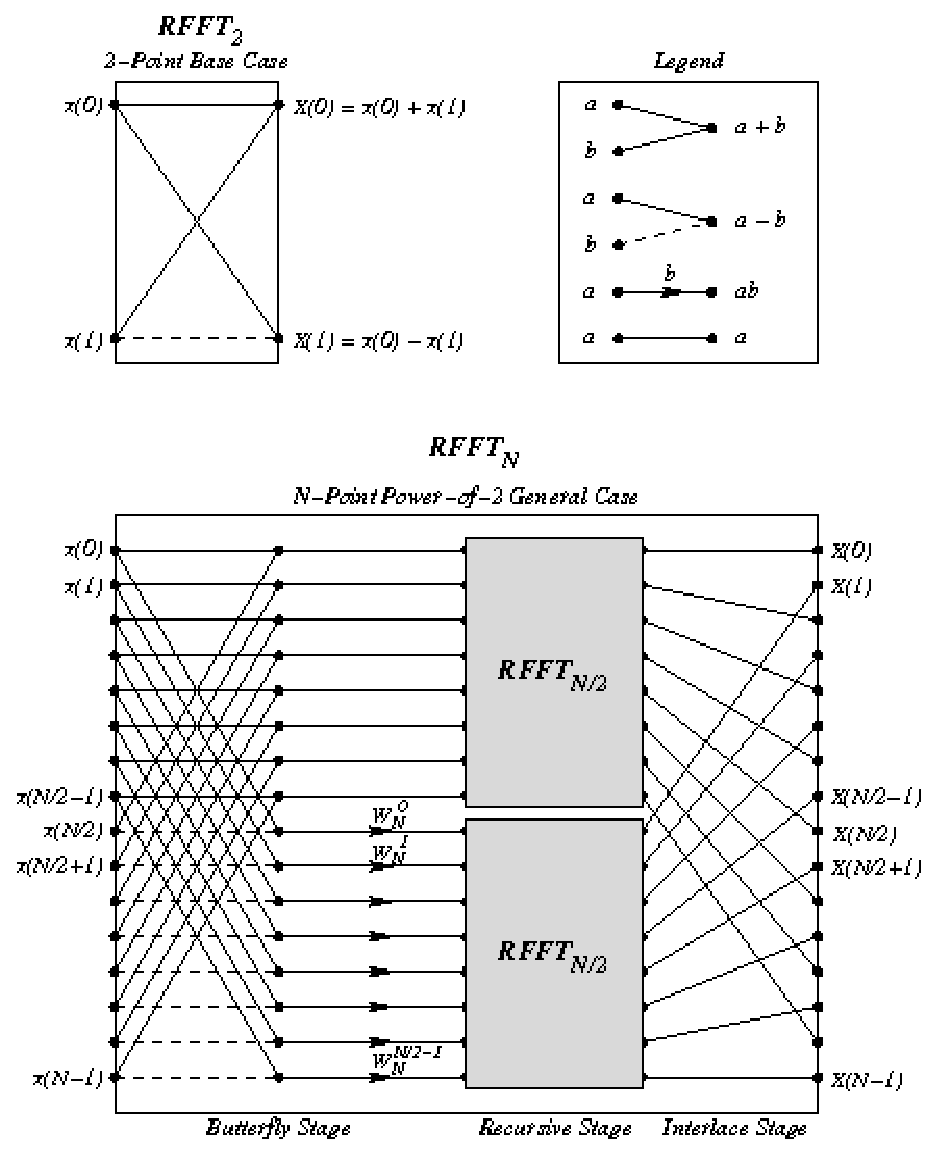
\includegraphics{math/45.eps}
\end{figure}



The diagram above is adapted from one by
Sam Daniel [\hyperref[bibliography_g225]{7}]
and shows the computational structure of the RFFT algorithm.
The first stage computes pairwise sums and differences
of the first and second halves of the input; this stage is labeled
the \textit{butterfly} stage.
The second stage recurs on the resulting subsequences.
The third stage interlaces the output of the
two recursive calls to RFFT, thus yielding the properly ordered
sequence \{\textit{X}(\textit{m})\}\textsubscript{\textit{m}=0}\textsuperscript{\textit{N}-1}.


The procedure \texttt{dft} accepts a sequence
(list) of values, \texttt{x}, the length of which
is assumed to be a power of 2.
\texttt{dft} precomputes a sequence of powers
of \(W_N\), \(\{W_N^n\}_{n=0}^{N/2-1}\), and calls \texttt{rfft} to
initiate the recursion.
\texttt{rfft} follows the algorithm outlined above.


\begin{alltt}
(define (dft x)
  (define (w-powers n)
    (let ([pi (* (acos 0.0) 2)])
      (let ([delta (/ (* -2.0i pi) n)])
        (let f ([n n] [x 0.0])
          (if (= n 0)
              '()
              (cons (exp x) (f (- n 2) (+ x delta))))))))
  (define (evens w)
    (if (null? w)
        '()
        (cons (car w) (evens (cddr w)))))
  (define (interlace x y)
    (if (null? x)
        '()
        (cons (car x) (cons (car y) (interlace (cdr x) (cdr y))))))
  (define (split ls)
    (let split ([fast ls] [slow ls])
      (if (null? fast)
          (values '() slow)
          (let-values ([(front back) (split (cddr fast) (cdr slow))])
            (values (cons (car slow) front) back)))))
  (define (butterfly x w)
    (let-values ([(front back) (split x)])
      (values
        (map + front back)
        (map * (map - front back) w))))
  (define (rfft x w)
    (if (null? (cddr x))
        (let ([x0 (car x)] [x1 (cadr x)])
          (list (+ x0 x1) (- x0 x1)))
        (let-values ([(front back) (butterfly x w)])
          (let ([w (evens w)])
            (interlace (rfft front w) (rfft back w))))))
  (rfft x (w-powers (length x))))
\end{alltt}

\paragraph{Exercise \label{examples_g199}12.9.1}


\label{examples_s71}Alter the algorithm to employ a base case of four points.
What simplifications can be made to avoid multiplying any of the
base case outputs by elements of \texttt{w}?


\paragraph{Exercise \label{examples_g200}12.9.2}


\label{examples_s72}Recode \texttt{dft} to accept a vector rather than a list as input, and
have it produce a vector as output.
Use lists internally if necessary, but do not simply convert the input to a
list on entry and the output to a vector on exit.


\paragraph{Exercise \label{examples_g201}12.9.3}


\label{examples_s73}Rather than recomputing the powers of \texttt{w} on each step for a new
number of points, the code simply uses the even-numbered elements of
the preceding list of powers.
Show that doing so yields the proper list of powers.
That is, show that \texttt{(evens (w-powers n))} is equal to
\texttt{(w-powers (/ n 2))}.


\paragraph{Exercise \label{examples_g202}12.9.4}


\label{examples_s74}The recursion step creates several intermediate lists that are
immediately discarded.
Recode the recursion step to avoid any unnecessary allocation.


\paragraph{Exercise \label{examples_g203}12.9.5}


\label{examples_s75}Each element of a sequence of input values may be regenerated from
the discrete Fourier transform of the sequence via the equation
\[X(n)=\frac{1}{N}\sum_{m=0}^{N-1}X(m)e^{i\frac{2\pi{}mn}{N}}\]
Noting the similarity between this equation and the original equation
defining \textit{X}(\textit{m}), create a modified version of \texttt{dft},
\texttt{inverse-dft}, that performs the inverse transformation.
Verify that \texttt{(inverse-dft (dft \textit{seq}))} returns
\texttt{\textit{seq}} for several input sequences \texttt{\textit{seq}}.

\section{\label{examples_g204}\label{examples_h10}A Unification Algorithm\label{examples_SECTEXUNIFY}}



\textit{Unification} [\hyperref[bibliography_g241]{23}] is a pattern-matching technique
used in automated theorem proving, type-inference systems, computer
algebra, and logic programming, e.g., Prolog [\hyperref[bibliography_g224]{6}].


A \label{examples_s76}unification algorithm attempts to make two symbolic expressions
equal by computing a unifying substitution for the expressions.
A \textit{substitution} is a function that replaces variables with other
expressions.
A substitution must treat all occurrences of a variable the same way,
e.g., if it replaces one occurrence of the variable \textit{x} by \textit{a}, it must
replace all occurrences of \textit{x} by \textit{a}.
A unifying substitution, or \textit{unifier}, for two expressions \textit{e}\textsubscript{1} and
\textit{e}\textsubscript{2} is a substitution, \(\sigma\), such that \(\sigma(e_1)=\sigma(e_2)\).


For example, the two expressions \textit{f}(\textit{x}) and \textit{f}(\textit{y}) can be unified by
substituting \textit{x} for \textit{y} (or \textit{y} for \textit{x}).
In this case, the unifier \(\sigma\) could be described as the function
that replaces \textit{y} with \textit{x} and leaves other variables unchanged.
On the other hand, the two expressions \textit{x} + 1 and \textit{y} + 2 cannot be
unified.
It might appear that substituting 3 for \textit{x} and 2 for \textit{y} would
make both expressions equal to 4 and hence equal to each other.
The symbolic expressions, 3 + 1 and 2 + 2, however, still differ.


Two expressions may have more than one unifier.
For example, the expressions \textit{f}(\textit{x},\textit{y}) and \textit{f}(1,\textit{y}) can be unified to
\textit{f}(1,\textit{y}) with the substitution of 1 for \textit{x}.
They may also be unified to \textit{f}(1,5) with the substitution of 1 for
\textit{x} and 5 for \textit{y}.
The first substitution is preferable, since it does not commit to
the unnecessary replacement of \textit{y}.
Unification algorithms typically produce the \textit{most general unifier},
or \textit{mgu}, for two expressions.
The mgu for two expressions makes no unnecessary substitutions; all
other unifiers for the expressions are special cases of the mgu.
In the example above, the first substitution is the mgu and the second
is a special case.


For the purposes of this program, a symbolic expression can be a variable,
a constant, or a function application.
Variables are represented by Scheme symbols, e.g., \texttt{x};
a function application is represented by a list with the function name in
the first position and its arguments in the remaining positions, e.g.,
\texttt{(f x)}; and
constants are represented by zero-argument functions, e.g., \texttt{(a)}.


The algorithm presented here finds the mgu for two terms, if it exists,
using a \label{examples_s77}continuation-passing style, or
CPS (see Section \ref{further_g75}),
approach to recursion on subterms.
The procedure \label{examples_s78}\texttt{unify} takes two terms and passes
them to a help procedure, \texttt{uni}, along with an initial (identity)
substitution, a success continuation, and a failure continuation.
The success continuation returns the result of applying its argument,
a substitution, to one of the terms, i.e., the unified result.
The failure continuation simply returns its argument, a message.
Because control passes by explicit continuation within \texttt{unify}
(always with tail calls), a return from the success or failure
continuation is a return from \texttt{unify} itself.


Substitutions are procedures.
Whenever a variable is to be replaced by another term, a new
substitution is formed from the variable, the term, and
the existing substitution.
Given a term as an argument, the new substitution replaces
occurrences of its saved variable with its saved term in the
result of invoking the saved substitution on the argument expression.
Intuitively, a substitution is a chain of procedures, one for each
variable in the substitution.
The chain is terminated by the initial, identity substitution.


\begin{alltt}
(unify 'x 'y) \(\Rightarrow\) y
(unify '(f x y) '(g x y)) \(\Rightarrow\) "clash"
(unify '(f x (h)) '(f (h) y)) \(\Rightarrow\) (f (h) (h))
(unify '(f (g x) y) '(f y x)) \(\Rightarrow\) "cycle"
(unify '(f (g x) y) '(f y (g x))) \(\Rightarrow\) (f (g x) (g x))
(unify '(f (g x) y) '(f y z)) \(\Rightarrow\) (f (g x) (g x))
\end{alltt}


\begin{alltt}
(library (tspl unification)
  (export unify)
  (import (rnrs))

 ; occurs? returns true if and only if u occurs in v
  (define occurs?
    (lambda (u v)
      (and (pair? v)
           (let f ([l (cdr v)])
             (and (pair? l)
                  (or (eq? u (car l))
                      (occurs? u (car l))
                      (f (cdr l))))))))

 ; sigma returns a new substitution procedure extending s by
 ; the substitution of u with v
  (define sigma
    (lambda (u v s)
      (lambda (x)
        (let f ([x (s x)])
          (if (symbol? x)
              (if (eq? x u) v x)
              (cons (car x) (map f (cdr x))))))))

 ; try-subst tries to substitute u for v but may require a
 ; full unification if (s u) is not a variable, and it may
 ; fail if it sees that u occurs in v.
  (define try-subst
    (lambda (u v s ks kf)
      (let ([u (s u)])
        (if (not (symbol? u))
            (uni u v s ks kf)
            (let ([v (s v)])
              (cond
                [(eq? u v) (ks s)]
                [(occurs? u v) (kf "cycle")]
                [else (ks (sigma u v s))]))))))

 ; uni attempts to unify u and v with a continuation-passing
 ; style that returns a substitution to the success argument
 ; ks or an error message to the failure argument kf.  The
 ; substitution itself is represented by a procedure from
 ; variables to terms.
  (define uni
    (lambda (u v s ks kf)

      (cond
        [(symbol? u) (try-subst u v s ks kf)]
        [(symbol? v) (try-subst v u s ks kf)]
        [(and (eq? (car u) (car v))
              (= (length u) (length v)))
         (let f ([u (cdr u)] [v (cdr v)] [s s])
           (if (null? u)
               (ks s)
               (uni (car u)
                    (car v)
                    s
                    (lambda (s) (f (cdr u) (cdr v) s))
                    kf)))]
        [else (kf "clash")])))

 ; unify shows one possible interface to uni, where the initial
 ; substitution is the identity procedure, the initial success
 ; continuation returns the unified term, and the initial failure
 ; continuation returns the error message.
  (define unify
    (lambda (u v)
      (uni u
           v
           (lambda (x) x)
           (lambda (s) (s u))
           (lambda (msg) msg)))))
\end{alltt}

\paragraph{Exercise \label{examples_g205}12.10.1}


\label{examples_s79}Modify \texttt{unify} so that it returns its substitution rather
than the unified term.
Apply this substitution to both input terms to verify that it
returns the same result for each.


\paragraph{Exercise \label{examples_g206}12.10.2}


\label{examples_s80}As mentioned above, substitutions on a term are performed
sequentially, requiring one entire pass through the input expression
for each substituted variable.
Represent the substitution differently so that only one pass
through the expression need be made.
Make sure that substitutions are performed not only on the input
expression but also on any expressions you insert during substitution.


\paragraph{Exercise \label{examples_g207}12.10.3}


\label{examples_s81}Extend the continuation-passing style unification algorithm into
an entire continuation-passing style logic programming system.



\section{\label{examples_g208}\label{examples_h11}Multitasking with Engines\label{examples_SECTEXENGINES}}



\label{examples_s82}Engines are a high-level process abstraction supporting
\label{examples_s83}\textit{timed
preemption} [\hyperref[bibliography_g228]{10},\hyperref[bibliography_g233]{15}].
Engines may be used to simulate \label{examples_s84}multiprocessing,
implement \label{examples_s85}\label{examples_s86}light-weight threads,
implement operating
system kernels, and perform \label{examples_s87}nondeterministic computations.
The engine implementation is one of the more interesting applications
of \label{examples_s88}continuations in Scheme.


An engine is created by passing a thunk (procedure of no arguments)
to the procedure \texttt{make-engine}.
The body of the thunk is the computation to be performed by the engine.
An engine itself is a procedure of three arguments:

\begin{enumerate}
\label{examples_g209}\item 
\label{examples_s89}\texttt{\textit{ticks}},
a positive integer that specifies the amount of \textit{fuel} to be given
to the engine.
An engine executes until this fuel runs out or until its computation
finishes.


\label{examples_g210}\item 
\label{examples_s90}\texttt{\textit{complete}},
a procedure of two arguments that
specifies what to do if the computation finishes.
Its arguments will be the amount of fuel left over and the
result of the computation.



\label{examples_g211}\item 
\label{examples_s91}\texttt{\textit{expire}},
a procedure of one argument that specifies what to do if the fuel runs
out before the computation finishes.
Its argument will be a new engine capable of continuing the computation
from the point of interruption.

\end{enumerate}


When an engine is applied to its arguments, it sets up a timer
to fire in \texttt{\textit{ticks}} time units.
If the engine computation completes before the timer goes off, the
system invokes \texttt{\textit{complete}}, passing it the
number of \texttt{\textit{ticks}} left over
and the value of the computation.
If, on the other hand, the timer goes off before the engine computation
completes, the system creates a new engine from the continuation of
the interrupted computation and passes this engine to \texttt{\textit{expire}}.
\texttt{\textit{complete}} and \texttt{\textit{expire}} are invoked in the continuation
of the engine invocation.


The following example creates an engine from a trivial computation,
3, and gives the engine 10 ticks.


\begin{alltt}
(define eng
  (make-engine
    (lambda () 3)))

(eng 10
  (lambda (ticks value) value)
  (lambda (x) x)) \(\Rightarrow\) 3
\end{alltt}


It is often useful to pass \texttt{list} as the \texttt{\textit{complete}} procedure
to an engine, causing the engine to return a list of the
ticks remaining and the value if the computation completes.


\begin{alltt}
(eng 10
  list
  (lambda (x) x)) \(\Rightarrow\) (9 3)
\end{alltt}


In the example above, the value was 3 and there were 9 ticks left over,
i.e., it took only one unit of fuel to evaluate 3.
(The fuel amounts given here are for illustration only.
The actual amount may differ.)


Typically, the engine computation does not finish in one try.
\label{examples_s92}The following example displays the use of an engine to
compute the 10th Fibonacci number (see Section \ref{further_g55})
in steps.


\begin{alltt}
(define fibonacci
  (lambda (n)
    (if (\textless{} n 2)
        n
        (+ (fibonacci (- n 1))
           (fibonacci (- n 2))))))

(define eng
  (make-engine
    (lambda ()
      (fibonacci 10))))

(eng 50
  list
  (lambda (new-eng)
    (set! eng new-eng)
    "expired")) \(\Rightarrow\) "expired"

(eng 50
  list
  (lambda (new-eng)
    (set! eng new-eng)
    "expired")) \(\Rightarrow\) "expired"

(eng 50
  list
  (lambda (new-eng)
    (set! eng new-eng)
    "expired")) \(\Rightarrow\) "expired"

(eng 50
  list
  (lambda (new-eng)
    (set! eng new-eng)
    "expired")) \(\Rightarrow\) (22 55)
\end{alltt}


Each time the engine's fuel ran out, the \texttt{\textit{expire}} procedure assigned
\texttt{eng} to the new engine.
The entire computation required four allotments of 50 ticks to complete; of the
last 50 it used all but 23.
Thus, the total amount of fuel used was 177 ticks.
This leads us to the following procedure, \texttt{mileage}, which
uses engines to ``time'' a computation.


\begin{alltt}
(define mileage
  (lambda (thunk)
    (let loop ([eng (make-engine thunk)] [total-ticks 0])
      (eng 50
        (lambda (ticks value)
          (+ total-ticks (- 50 ticks)))
        (lambda (new-eng)
          (loop new-eng (+ total-ticks 50)))))))

(mileage (lambda () (fibonacci 10))) \(\Rightarrow\) 178
\end{alltt}


The choice of 50 for the number of ticks to use each time is
arbitrary, of course.
It might make more sense to pass a much larger number, say 10000,
in order to reduce the number of times the computation is interrupted.


The next procedure, \label{examples_s93}\texttt{round-robin}, could be the basis for a simple
time-sharing \label{examples_s94}operating system.
\texttt{round-robin} maintains a queue of processes (a list of engines)
and cycles through the queue in a \textit{round-robin} fashion, allowing each
process to run for a set amount of time.
\texttt{round-robin} returns a list of the values returned by the engine
computations in the order that the computations complete.


\begin{alltt}
(define round-robin
  (lambda (engs)
    (if (null? engs)
        '()
        ((car engs) 1
          (lambda (ticks value)
            (cons value (round-robin (cdr engs))))
          (lambda (eng)
            (round-robin
              (append (cdr engs) (list eng))))))))
\end{alltt}


Assuming the amount of computation corresponding to one tick is constant,
the effect of \texttt{round-robin} is to return a list of the values sorted
from the quickest to complete to the slowest to complete.
Thus, when we call \texttt{round-robin} on a list of engines, each computing
one of the Fibonacci numbers, the output list is sorted with the earlier
Fibonacci numbers first, regardless of the order of the input list.


\begin{alltt}
(round-robin
  (map (lambda (x)
         (make-engine
           (lambda ()
              (fibonacci x))))
       '(4 5 2 8 3 7 6 2))) \(\Rightarrow\) (1 1 2 3 5 8 13 21)
\end{alltt}


More interesting things could happen if the amount of fuel varied
each time through the loop.
\label{examples_s95}In this case, the computation would
be nondeterministic, i.e., the results would vary from call to call.


The following syntactic form, \label{examples_s96}\texttt{por} (parallel-or), returns the
first of its expressions to complete with a true value.
\texttt{por} is implemented with the procedure \texttt{first-true}, which is
similar to \texttt{round-robin} but quits when any of the engines
completes with a true value.
If all of the engines complete, but none with a true value,
\texttt{first-true} (and hence \texttt{por}) returns \texttt{\#{}f}.


\begin{alltt}
(define-syntax por
  (syntax-rules ()
    [(\_{} x ...)
     (first-true
       (list (make-engine (lambda () x)) ...))]))

(define first-true
  (lambda (engs)
    (if (null? engs)
        \#{}f
        ((car engs) 1
          (lambda (ticks value)
            (or value (first-true (cdr engs))))
          (lambda (eng)
            (first-true
              (append (cdr engs) (list eng))))))))
\end{alltt}


Even if one of the expressions is an infinite loop,
\texttt{por} can still finish (as long as one of the other expressions
completes and returns a true value).


\begin{alltt}
(por 1 2) \(\Rightarrow\) 1
(por ((lambda (x) (x x)) (lambda (x) (x x)))
     (fibonacci 10)) \(\Rightarrow\) 55
\end{alltt}


The first subexpression of the second \texttt{por} expression is
nonterminating, so the answer is the value of the second
subexpression.


Let's turn to the implementation of engines.
Any preemptive multitasking primitive must have the ability to
interrupt a running process after a given amount of computation.
This ability is provided by a primitive \label{examples_s97}timer
interrupt mechanism in some Scheme implementations.
We will construct a suitable one here.


Our timer system defines three procedures: \texttt{start-timer}, \texttt{stop-timer},
and \texttt{decrement-timer}, which can be described operationally as
follows.

\begin{itemize}
\item 
\texttt{(start-timer \textit{ticks} \textit{handler})}
sets the timer
to \texttt{\textit{ticks}} and installs \texttt{\textit{handler}} as the procedure to be
invoked (without arguments) when the timer expires, i.e., reaches zero.

\item 
\texttt{(stop-timer)}
resets the timer and returns the number of ticks remaining.

\item 
\texttt{(decrement-timer)}
decrements the timer by one tick if the timer is on, i.e., if it is
not zero.
When the timer reaches zero, \texttt{decrement-timer} invokes the saved
handler.
If the timer has already reached zero, \texttt{decrement-timer} returns
without changing the timer.

\end{itemize}


Code to implement these procedures is given along with the engine
implementation below.


Using the timer system requires inserting calls to \texttt{decrement-timer} in
appropriate places.
Consuming a timer tick on entry to a procedure usually provides a sufficient
level of granularity.
This can be accomplished by using \texttt{timed-lambda} as defined below
in place of \texttt{lambda}.
\texttt{timed-lambda} simply invokes \texttt{decrement-timer} before executing the
expressions in its body.


\begin{alltt}
(define-syntax timed-lambda
  (syntax-rules ()
    [(\_{} formals exp1 exp2 ...)
     (lambda formals (decrement-timer) exp1 exp2 ...)]))
\end{alltt}


It may be useful to redefine named \texttt{let} and \texttt{do} to use \texttt{timed-lambda}
as well, so that recursions expressed with these constructs are
timed.
If you use this mechanism, do not forget to use the timed versions of
\texttt{lambda} and other forms in code run within an engine, or no
ticks will be consumed.


Now that we have a suitable timer, we can implement engines in terms of
the timer and continuations.
We use \label{examples_s98}\texttt{call/cc} in two places in the engine
implementation: (1) to obtain the continuation of the computation that invokes
the engine so that we can return to that continuation when the engine
computation completes or the timer expires, and (2) to obtain the continuation
of the engine computation when the timer expires so that we can return
to this computation if the newly created engine is subsequently run.


The state of the engine system is contained in two variables local to
the engine system: \texttt{do-complete} and \texttt{do-expire}.
When an engine is started, the engine assigns to \texttt{do-complete} and
\texttt{do-expire} procedures
that, when invoked, return to the continuation of the engine's caller
to invoke \texttt{\textit{complete}} or \texttt{\textit{expire}}.
The engine starts (or restarts) the computation by invoking
the procedure passed as an argument to \texttt{make-engine} with the specified
number of ticks.
The ticks and the local procedure \texttt{timer-handler} are then used to
start the timer.


Suppose that the timer expires before the engine computation completes.
The procedure \texttt{timer-handler} is then invoked.
It initiates a call to \texttt{start-timer} but obtains the ticks by calling
\texttt{call/cc} with \texttt{do-expire}.
Consequently, \texttt{do-expire} is
called with a continuation that, if invoked,
will restart the timer and continue the interrupted computation.
\texttt{do-expire} creates a new engine from this continuation and
arranges for the engine's \texttt{\textit{expire}} procedure to be invoked with the new
engine in the correct continuation.


If, on the other hand, the engine computation completes before
the timer expires, the timer is stopped and the number of ticks remaining
is passed along with the value to \texttt{do-complete};
\texttt{do-complete} arranges for the engine's \texttt{\textit{complete}} procedure
to be invoked with the ticks and value in the correct continuation.


Let's discuss a couple of subtle aspects to this code.
The first concerns the method used to start the timer when an engine
is invoked.
The code would apparently be simplified by letting \texttt{new-engine} start
the timer before it initiates or resumes the engine computation, instead
of passing the ticks to the computation and letting it start the timer.
Starting the timer within the computation, however, prevents ticks from
being consumed prematurely.
If the engine system itself consumes fuel, then an engine provided with a
small amount of fuel may not progress toward completion.
(It may, in fact, make negative progress.)
If the software timer described above is used, this problem is actually
avoided by compiling the engine-making code with the untimed version of
\texttt{lambda}.


The second subtlety concerns the procedures created by \texttt{do-complete} and
\texttt{do-expire} and subsequently applied by the continuation of the
\label{examples_s99}\label{examples_s100}\texttt{call/cc} application.
It may appear that \texttt{do-complete} could first invoke the engine's
\texttt{\textit{complete}} procedure, then pass the result to the continuation
(and similarly for \texttt{do-expire}) as follows.


\texttt{(escape (complete value ticks))}

This would result in improper treatment of tail recursion, however.
The problem is that the current continuation would not be replaced with the
continuation stored in \texttt{escape} until the call to the \texttt{complete}
procedure returns.
Consequently, both the continuation of the running engine and the continuation
of the engine invocation could be retained for an indefinite period of time,
when in fact the actual engine invocation may appear to be tail-recursive.
This is especially inappropriate because the engine interface encourages use of
continuation-passing style and hence tail recursion.
The round-robin scheduler and \texttt{first-true} provide good examples of this,
since the \texttt{\textit{expire}} procedure in each invokes engines tail-recursively.


We maintain proper treatment of tail recursion by arranging for
\texttt{do-complete} and \texttt{do-expire} to escape from
the continuation of the running engine before invoking the \texttt{complete} or
\texttt{expire} procedures.
Since the continuation of the engine invocation is a procedure application,
passing it a procedure of no arguments results in application of the procedure
in the continuation of the engine invocation.


\begin{alltt}
(library (tspl timer)
  (export start-timer stop-timer decrement-timer)
  (import (rnrs))

  (define clock 0)
  (define handler \#{}f)

  (define start-timer
    (lambda (ticks new-handler)
      (set! handler new-handler)
      (set! clock ticks)))

  (define stop-timer
    (lambda ()
      (let ([time-left clock])
        (set! clock 0)
        time-left)))

  (define decrement-timer
    (lambda ()
      (when (\textgreater{} clock 0)
        (set! clock (- clock 1))
        (when (= clock 0) (handler)))))

  (define-syntax timed-lambda
    (syntax-rules ()
      [(\_{} formals exp1 exp2 ...)
       (lambda formals (decrement-timer) exp1 exp2 ...)])))

(library (tspl engines)
  (export make-engine timed-lambda)
  (import (rnrs) (tspl timer))

  (define make-engine
    (let ([do-complete \#{}f] [do-expire \#{}f])
      (define timer-handler
        (lambda ()
          (start-timer (call/cc do-expire) timer-handler)))
      (define new-engine
        (lambda (resume)
          (lambda (ticks complete expire)
            ((call/cc
               (lambda (escape)
                 (set! do-complete
                   (lambda (ticks value)
                     (escape (lambda () (complete ticks value)))))
                 (set! do-expire
                   (lambda (resume)
                     (escape (lambda ()
                               (expire (new-engine resume))))))
                 (resume ticks)))))))
      (lambda (proc)
        (new-engine
          (lambda (ticks)
            (start-timer ticks timer-handler)
            (let ([value (proc)])
              (let ([ticks (stop-timer)])
                (do-complete ticks value))))))))

  (define-syntax timed-lambda
    (syntax-rules ()
      [(\_{} formals exp1 exp2 ...)
       (lambda formals (decrement-timer) exp1 exp2 ...)])))
\end{alltt}

\paragraph{Exercise \label{examples_g212}12.11.1}


\label{examples_s101}If your Scheme implementation allows definition and import of libraries
in the interactive top level, try defining the libraries above, then
type


\texttt{(import (rename (tspl engines) (timed-lambda lambda)))}

to define \texttt{make-engine} and redefine \texttt{lambda}.
Then try out the examples given earlier in this section.


\paragraph{Exercise \label{examples_g213}12.11.2}


\label{examples_s102}It may appear that the nested \texttt{let} expressions in the body of
\texttt{make-engine}:


\begin{alltt}
(let ([value (proc)])
  (let ([ticks (stop-timer)])
    (do-complete ticks value)))
\end{alltt}


could be replaced with the following.


\begin{alltt}
(let ([value (proc)] [ticks (stop-timer)])
  (do-complete value ticks))
\end{alltt}


Why is this not correct?


\paragraph{Exercise \label{examples_g214}12.11.3}


\label{examples_s103}It would also be incorrect to replace the
nested \texttt{let} expressions discussed in the preceding exercise
with the following.


\begin{alltt}
(let ([value (proc)])
  (do-complete value (stop-timer)))
\end{alltt}


Why?


\paragraph{Exercise \label{examples_g215}12.11.4}


\label{examples_s104}Modify the engine implementation to provide a procedure,
\texttt{engine-return}, that returns immediately from an engine.


\paragraph{Exercise \label{examples_g216}12.11.5}


\label{examples_s105}Implement the kernel of a small \label{examples_s106}operating
system using engines for processes.
Processes should request services (such as reading input from the user)
by evaluating an expression of the form \texttt{(trap 'request)}.
Use \texttt{call/cc} and \texttt{engine-return} from the preceding
exercise to implement \texttt{trap}.


\paragraph{Exercise \label{examples_g217}12.11.6}


\label{examples_s107}Write the same operating-system kernel without using engines, building
instead from continuations and timer interrupts.


\paragraph{Exercise \label{examples_g218}12.11.7}


\label{examples_s108}This implementation of engines does not allow one engine to call
another, i.e., nested engines [\hyperref[bibliography_g228]{10}].
Modify the implementation to allow \label{examples_s109}nested
engines.





\SpecialChapter{References}

\label{bibliography_h0}





\noindent[\label{bibliography_g219}1] 
Michael Adams and R. Kent Dybvig.
Efficient nondestructive equality checking for trees and graphs.
In \textit{Proceedings of the 13th ACM SIGPLAN International
  Conference on Functional Programming},  179-188, September 2008.


\noindent[\label{bibliography_g220}2] 
J. Michael Ashley and R. Kent Dybvig.
An efficient implementation of multiple return values in Scheme.
In \textit{Proceedings of the 1994 ACM Conference on Lisp and
  Functional Programming},  140-149, June 1994.


\noindent[\label{bibliography_g221}3] 
Alan Bawden.
Quasiquotation in lisp.
In \textit{Partial Evaluation and Semantic-Based Program Manipulation},
   88-99, 1999.


\noindent[\label{bibliography_g222}4] 
William Briggs and Van Emden Henson.
\textit{The DFT: An Owner's Manual for the Discrete Fourier
  Transform}.
Society for Industrial and Applied Mathematics, Philadelphia, PA,
  1995.


\noindent[\label{bibliography_g223}5] 
Robert G. Burger and R. Kent Dybvig.
Printing floating-point numbers quickly and accurately.
In \textit{Proceedings of the ACM SIGPLAN '96 Conference on
  Programming Language Design and Implementation},  108-116, May 1996.


\noindent[\label{bibliography_g224}6] 
William F. Clocksin and Christopher S. Mellish.
\textit{Programming in Prolog}, second edition.
Springer-Verlag, Berlin, 1984.


\noindent[\label{bibliography_g225}7] 
Sam M. Daniel.
Efficient recursive FFT implementation in Prolog.
In \textit{Proceedings of the Second International Conference on the
  Practical Application of Prolog},  175-185, 1994.


\noindent[\label{bibliography_g226}8] 
Mark Davis.
Unicode Standard Annex \#{}29: Text boundaries, 2006.
 \textit{http://www.unicode.org/reports/tr29/}.
 
\noindent[\label{bibliography_g227}9] 
R. Kent Dybvig.
\textit{Chez Scheme User's Guide: Version 8}.
Cadence Research Systems, 2009.
 \textit{http://www.scheme.com/csug8/}.
 
\noindent[\label{bibliography_g228}10] 
R. Kent Dybvig and Robert Hieb.
Engines from continuations.
\textit{Computer Languages}, 14(2):109-123, 1989.


\noindent[\label{bibliography_g229}11] 
R. Kent Dybvig and Robert Hieb.
A new approach to procedures with variable arity.
\textit{Lisp and Symbolic Computation}, 3(3):229-244, September
  1990.


\noindent[\label{bibliography_g230}12] 
R. Kent Dybvig, Robert Hieb, and Carl Bruggeman.
Syntactic abstraction in Scheme.
\textit{Lisp and Symbolic Computation}, 5(4):295-326, 1993.


\noindent[\label{bibliography_g231}13] 
Daniel P. Friedman and Matthias Felleisen.
\textit{The Little Schemer}, fourth edition.
MIT Press, Cambridge, MA, 1996.


\noindent[\label{bibliography_g232}14] 
Daniel P. Friedman, Christopher T. Haynes, and Eugene E. Kohlbecker.
Programming with continuations.
In P. Pepper, editor, \textit{Program Transformation and Programming
  Environments},  263-274. Springer-Verlag, New York, 1984.


\noindent[\label{bibliography_g233}15] 
Christopher T. Haynes and Daniel P. Friedman.
Abstracting timed preemption with engines.
\textit{Computer Languages}, 12(2):109-121, 1987.


\noindent[\label{bibliography_g234}16] 
Christopher T. Haynes, Daniel P. Friedman, and Mitchell Wand.
Obtaining coroutines with continuations.
\textit{Computer Languages}, 11(3/4):143-153, 1986.


\noindent[\label{bibliography_g235}17] 
Robert Hieb, R. Kent Dybvig, and Carl Bruggeman.
Representing control in the presence of first-class continuations.
In \textit{Proceedings of the SIGPLAN '90 Conference on Programming
  Language Design and Implementation},  66-77, June 1990.


\noindent[\label{bibliography_g236}18] 
IEEE Computer Society.
\textit{IEEE Standard for the Scheme Programming Language}, May
  1991.
IEEE Std 1178-1990.


\noindent[\label{bibliography_g237}19] 
Brian W. Kernighan and Dennis M. Ritchie.
\textit{The C Programming Language}, second edition.
Prentice Hall, Englewood Cliffs, NJ, 1988.


\noindent[\label{bibliography_g238}20] 
P. Leach, M. Mealling, and R. Salz.
A Universally Unique IDentifier (UUID) URN namespace, July
  2005.
RFC 4122.
 \textit{http://www.ietf.org/rfc/rfc4122.txt}.

\noindent[\label{bibliography_g239}21] 
Peter Naur et al.
Revised report on the algorithmic language ALGOL 60.
\textit{Communications of the ACM}, 6(1):1-17, January 1963.


\noindent[\label{bibliography_g240}22] 
David A. Plaisted.
Constructs for sets, quantifiers, and rewrite rules in Lisp.
Technical Report UIUCDCS-R-84-1176, University of Illinois at
  Urbana-Champaign Department of Computer Science, June 1984.


\noindent[\label{bibliography_g241}23] 
J. A. Robinson.
A machine-oriented logic based on the resolution principle.
\textit{Journal of the ACM}, 12(1):23-41, 1965.


\noindent[\label{bibliography_g242}24] 
Michael Sperber, R. Kent Dybvig, Matthew Flatt, and Anton van Straaten (eds.).
Revised\textsuperscript{6} report on the algorithmic language Scheme, September
  2007.
 \textit{http://www.r6rs.org/}.
 
\noindent[\label{bibliography_g243}25] 
Michael Sperber, R. Kent Dybvig, Matthew Flatt, and Anton van Straaten (eds.).
Revised\textsuperscript{6} report on the algorithmic language
  Scheme---non-normative appendices, September 2007.
 \textit{http://www.r6rs.org/}.
 
\noindent[\label{bibliography_g244}26] 
Michael Sperber, R. Kent Dybvig, Matthew Flatt, and Anton van Straaten (eds.).
Revised\textsuperscript{6} report on the algorithmic language Scheme---standard
  libraries, September 2007.
 \textit{http://www.r6rs.org/}.
 
\noindent[\label{bibliography_g245}27] 
Guy L. Steele Jr.
\textit{Common Lisp, the Language}, second edition.
Digital Press, Bedford, Massachusetts, 1990.


\noindent[\label{bibliography_g246}28] 
Guy L. Steele Jr. and Gerald J. Sussman.
The revised report on Scheme, a dialect of Lisp.
MIT AI Memo 452, Massachusetts Institute of Technology, January 1978.


\noindent[\label{bibliography_g247}29] 
Gerald J. Sussman and Guy L. Steele Jr.
Scheme: An interpreter for extended lambda calculus.
\textit{Higher-Order and Symbolic Computation}, 11(4):405-439, 1998.
Reprinted from the AI Memo 349, MIT (1975), with a foreword.


\noindent[\label{bibliography_g248}30] 
The Unicode Consortium.
\textit{The Unicode Standard, Version 5.0}, fifth edition.
Addison-Wesley Professional, Boston, MA, 2006.


\noindent[\label{bibliography_g249}31] 
Oscar Waddell, Dipanwita Sarkar, and R. Kent Dybvig.
Fixing letrec: A faithful yet efficient implementation of Scheme's
  recursive binding construct.
\textit{Higher-Order and Symbolic Computation}, 18(3/4):299-326, 2005.


\noindent[\label{bibliography_g250}32] 
Mitchell Wand.
Continuation-based multiprocessing.
\textit{Higher-Order and Symbolic Computation}, 12(3):285-299, 1999.
Reprinted from the proceedings of the 1980 Lisp Conference, with a
  foreword.






\SpecialChapter{Answers to Selected Exercises}

\label{answers_h0}




  

\paragraph{Exercise \hyperref[start_g7]{2.2.1}. }(page \pageref{start_s34})

   
 
 \begin{enumerate}[\it a. ]
\item \texttt{(+ (* 1.2 (- 2 1/3)) -8.7)} \item \texttt{(/ (+ 2/3 4/9) (- 5/11 4/3))} \item \texttt{(+ 1 (/ 1 (+ 2 (/ 1 (+ 1 1/2)))))} \item \texttt{(* (* (* (* (* (* 1 -2) 3) -4) 5) -6) 7)} or       \texttt{(* 1 -2 3 -4 5 -6 7)} \end{enumerate}
 


\paragraph{Exercise \hyperref[start_g8]{2.2.2}. }(page \pageref{start_s35})

  See Section \ref{objects_g110}. 


\paragraph{Exercise \hyperref[start_g9]{2.2.3}. }(page \pageref{start_s36})

   
 
 \begin{enumerate}[\it a. ]
\item \texttt{(car . cdr)} \item \texttt{(this (is silly))} \item \texttt{(is this silly?)} \item \texttt{(+ 2 3)} \item \texttt{(+ 2 3)} \item \texttt{+} \item \texttt{(2 3)} \item \texttt{\#{}\textless{}procedure\textgreater{}} \item \texttt{cons} \item \texttt{'cons} \item \texttt{quote} \item \texttt{5} \item \texttt{5} \item \texttt{5} \item \texttt{5} \end{enumerate}
 


\paragraph{Exercise \hyperref[start_g10]{2.2.4}. }(page \pageref{start_s37})

  
\begin{alltt}
 (car (cdr (car '((a b) (c d))))) \(\Rightarrow\) b
 (car (car (cdr '((a b) (c d))))) \(\Rightarrow\) c
 (car (cdr (car (cdr '((a b) (c d)))))) \(\Rightarrow\) d
\end{alltt}



\paragraph{Exercise \hyperref[start_g11]{2.2.5}. }(page \pageref{start_s38})

  
\texttt{ '((a . b) ((c) d) ())}


\paragraph{Exercise \hyperref[start_g12]{2.2.6}. }(page \pageref{start_s39})

  \begin{figure}[H]
\centering
%\includegraphics{math/50.eps}
\begin{tikzpicture}[start chain]

\node[list,on chain] (A1) {$1$ \nodepart{two} \phantom{null}};
\node[list,on chain] (A2) {\phantom{null} \nodepart{two} \phantom{null}};
\node[list,on chain] (A3) {\phantom{null} \nodepart{two} \phantom{null}};
\node[list,on chain] (A4) {$4$ \nodepart{two} $5$};

\node[list,below=of A3] (B1) {\texttt{()} \nodepart{two} \texttt{()}};

\node[list,below left=of B1] (C1) {$2$ \nodepart{two} \phantom{null}};
\node[list,right=of C1] (C2) {\phantom{null} \nodepart{two} \texttt{()}};

\node[list,below=of C2] (D1) {$3$ \nodepart{two} \texttt{()}};
  
\pSF{A1}{A2};
\pSF{A2}{A3};
\pSF{A3}{A4};

\pSF{C1}{C2};

\pFF{A2}{C1};
\pFF{A3}{B1};
\pFF{C2}{D1};

\end{tikzpicture}
\end{figure}
 


\paragraph{Exercise \hyperref[start_g13]{2.2.7}. }(page \pageref{start_s40})

  
\begin{alltt}
 (car '((a b) (c d))) \(\Rightarrow\) (a b)
 (car (car '((a b) (c d)))) \(\Rightarrow\) a
 (cdr (car '((a b) (c d)))) \(\Rightarrow\) (b)
 (car (cdr (car '((a b) (c d))))) \(\Rightarrow\) b
 (cdr (cdr (car '((a b) (c d))))) \(\Rightarrow\) ()
 (cdr '((a b) (c d))) \(\Rightarrow\) ((c d))
 (car (cdr '((a b) (c d)))) \(\Rightarrow\) (c d)
 (car (car (cdr '((a b) (c d))))) \(\Rightarrow\) c
 (cdr (car (cdr '((a b) (c d))))) \(\Rightarrow\) (d)
 (car (cdr (car (cdr '((a b) (c d)))))) \(\Rightarrow\) d
 (cdr (cdr (car (cdr '((a b) (c d)))))) \(\Rightarrow\) ()
 (cdr (cdr '((a b) (c d)))) \(\Rightarrow\) ()
\end{alltt}



\paragraph{Exercise \hyperref[start_g14]{2.2.8}. }(page \pageref{start_s41})

  See Section \ref{start_g15}. 


\paragraph{Exercise \hyperref[start_g16]{2.3.1}. }(page \pageref{start_s49})

   \begin{enumerate}  \label{answers_g251}\item 
Evaluate the variables \texttt{list}, \texttt{+}, \texttt{-}, \texttt{*}, and \texttt{/}, yielding        the list, addition, subtraction, multiplication, and division procedures.  \label{answers_g252}\item \label{answers_listapply}Apply the list procedure to the addition, subtraction, multiplication, and division procedures,        yielding a list containing these procedures in order.  \label{answers_g253}\item Evaluate the variable \texttt{cdr}, yielding the cdr procedure.  \label{answers_g254}\item \label{answers_cdrapply}Apply the cdr procedure to the list produced in step \hyperref[answers_g252]{2},        yielding a list containing the subtraction, multiplication, and        division procedures.  \label{answers_g255}\item Evaluate the variable \texttt{car}, yielding the car procedure.  \label{answers_g256}\item Apply the car procedure to the list produced in step \hyperref[answers_g254]{4},        yielding the subtraction procedure.  \label{answers_g257}\item Evaluate the constants \texttt{17} and \texttt{5}, yielding        \texttt{17} and \texttt{5}.  \label{answers_g258}\item Apply the subtraction procedure to \texttt{17} and \texttt{5},        yielding \texttt{12}. \end{enumerate}
 
Other orders are possible.  For example, the variable \texttt{car} could have been evaluated before its argument. 



\paragraph{Exercise \hyperref[start_g18]{2.4.1}. }(page \pageref{start_s57})

   
 
 \begin{enumerate}[\it a. ]
\item \texttt{(let ([x (* 3 a)]) (+ (- x b) (+ x b)))} \item \texttt{(let ([x (list a b c)]) (cons (car x) (cdr x)))} \end{enumerate}
 


\paragraph{Exercise \hyperref[start_g19]{2.4.2}. }(page \pageref{start_s58})

  The value is 54. The outer \texttt{let} binds \texttt{x} to 9, while the inner \texttt{let} binds \texttt{x} to 3 (9/3). The inner \texttt{let} evaluates to 6 (3 + 3), and the outer \texttt{let} evaluates to 54 (9 \(\times\) 6). 


\paragraph{Exercise \hyperref[start_g20]{2.4.3}. }(page \pageref{start_s59})

   
 
 \begin{enumerate}[\it a. ]
\item 
\begin{alltt}
(let ([x0 'a] [y0 'b])
   (list (let ([x1 'c]) (cons x1 y0))
         (let ([y1 'd]) (cons x0 y1))))
\end{alltt}

\item 
\begin{alltt}
(let ([x0 '((a b) c)])
   (cons (let ([x1 (cdr x0)])
           (car x1))
         (let ([x2 (car x0)])
           (cons (let ([x3 (cdr x2)])
                   (car x3))
                 (cons (let ([x4 (car x2)])
                         x4)
                       (cdr x2))))))
\end{alltt}

\end{enumerate}
 


\paragraph{Exercise \hyperref[start_g22]{2.5.1}. }(page \pageref{start_s72})

   
 
 \begin{enumerate}[\it a. ]
\item \texttt{a} \item \texttt{(a)} \item \texttt{a} \item \texttt{()} \end{enumerate}
 


\paragraph{Exercise \hyperref[start_g23]{2.5.2}. }(page \pageref{start_s73})

  See page \pageref{start_defn_list}. 


\paragraph{Exercise \hyperref[start_g24]{2.5.3}. }(page \pageref{start_s74})

   
 
 \begin{enumerate}[\it a. ]
\item no free variables \item \texttt{+} \item \texttt{f} \item \texttt{cons}, \texttt{f}, and \texttt{y} \item \texttt{cons} and \texttt{y} \item \texttt{cons}, \texttt{y}, and \texttt{z} (\texttt{y} also       appears as a bound variable) \end{enumerate}
 


\paragraph{Exercise \hyperref[start_g26]{2.6.1}. }(page \pageref{start_s91})

  The program would loop indefinitely. 


\paragraph{Exercise \hyperref[start_g27]{2.6.2}. }(page \pageref{start_s92})

  
\begin{alltt}
 (define compose
   (lambda (p1 p2)
     (lambda (x)
       (p1 (p2 x))))) 

(define cadr (compose car cdr))
 (define cddr (compose cdr cdr))
\end{alltt}



\paragraph{Exercise \hyperref[start_g28]{2.6.3}. }(page \pageref{start_s96})

  
\begin{alltt}
 (define caar (compose car car))
 (define cadr (compose car cdr)) 

(define cdar (compose cdr car))
 (define cddr (compose cdr cdr)) 

(define caaar (compose car caar))
 (define caadr (compose car cadr))
 (define cadar (compose car cdar))
 (define caddr (compose car cddr)) 

(define cdaar (compose cdr caar))
 (define cdadr (compose cdr cadr))
 (define cddar (compose cdr cdar))
 (define cdddr (compose cdr cddr)) 

(define caaaar (compose caar caar))
 (define caaadr (compose caar cadr))
 (define caadar (compose caar cdar))
 (define caaddr (compose caar cddr))
 (define cadaar (compose cadr caar))
 (define cadadr (compose cadr cadr))
 (define caddar (compose cadr cdar))
 (define cadddr (compose cadr cddr)) 

(define cdaaar (compose cdar caar))
 (define cdaadr (compose cdar cadr))
 (define cdadar (compose cdar cdar))
 (define cdaddr (compose cdar cddr))
 (define cddaar (compose cddr caar))
 (define cddadr (compose cddr cadr))
 (define cdddar (compose cddr cdar))
 (define cddddr (compose cddr cddr))
\end{alltt}



\paragraph{Exercise \hyperref[start_g30]{2.7.1}. }(page \pageref{start_s126})

  
\begin{alltt}
 (define atom?
   (lambda (x)
     (not (pair? x))))
\end{alltt}



\paragraph{Exercise \hyperref[start_g31]{2.7.2}. }(page \pageref{start_s128})

  
\begin{alltt}
 (define shorter
   (lambda (ls1 ls2)
     (if (\textless{} (length ls2) (length ls1))
         ls2
         ls1)))
\end{alltt}



\paragraph{Exercise \hyperref[start_g33]{2.8.1}. }(page \pageref{start_s149})

  The structure of the output would be the mirror image of the structure of the input. For example, \texttt{(a . b)} would become \texttt{(b . a)} and \texttt{((a . b) . (c . d))} would become \texttt{((d . c) . (b . a))}. 


\paragraph{Exercise \hyperref[start_g34]{2.8.2}. }(page \pageref{start_s150})

  
\begin{alltt}
 (define append
   (lambda (ls1 ls2)
     (if (null? ls1)
         ls2
         (cons (car ls1) (append (cdr ls1) ls2)))))
\end{alltt}



\paragraph{Exercise \hyperref[start_g35]{2.8.3}. }(page \pageref{start_s152})

  
\begin{alltt}
 (define make-list
   (lambda (n x)
     (if (= n 0)
         '()
         (cons x (make-list (- n 1) x)))))
\end{alltt}



\paragraph{Exercise \hyperref[start_g36]{2.8.4}. }(page \pageref{start_s154})

  See the description of \texttt{list-ref} on page \pageref{objects_defn_list_ref} and the description of \texttt{list-tail} on page \pageref{objects_defn_list_tail}. 


\paragraph{Exercise \hyperref[start_g37]{2.8.5}. }(page \pageref{start_s155})

  
\begin{alltt}
 (define shorter?
   (lambda (ls1 ls2)
     (and (not (null? ls2))
          (or (null? ls1)
              (shorter? (cdr ls1) (cdr ls2)))))) 

(define shorter
   (lambda (ls1 ls2)
     (if (shorter? ls2 ls1)
         ls2
         ls1)))
\end{alltt}



\paragraph{Exercise \hyperref[start_g38]{2.8.6}. }(page \pageref{start_s158})

  
\begin{alltt}
 (define even?
   (lambda (x)
     (or (= x 0)
         (odd? (- x 1)))))
 (define odd?
   (lambda (x)
     (and (not (= x 0))
          (even? (- x 1)))))
\end{alltt}



\paragraph{Exercise \hyperref[start_g39]{2.8.7}. }(page \pageref{start_s161})

  
\begin{alltt}
 (define transpose
   (lambda (ls)
     (cons (map car ls) (map cdr ls))))
\end{alltt}



\paragraph{Exercise \hyperref[start_g41]{2.9.1}. }(page \pageref{start_s186})

  
\begin{alltt}
 (define make-counter
   (lambda (init incr)
     (let ([next init])
       (lambda ()
         (let ([v next])
           (set! next (+ next incr))
           v)))))
\end{alltt}



\paragraph{Exercise \hyperref[start_g42]{2.9.2}. }(page \pageref{start_s188})

  
\begin{alltt}
 (define make-stack
   (lambda ()
     (let ([ls '()])
       (lambda (msg . args)
         (case msg
           [(empty? mt?) (null? ls)]
           [(push!) (set! ls (cons (car args) ls))]
           [(top) (car ls)]
           [(pop!) (set! ls (cdr ls))]
           [else "oops"])))))
\end{alltt}



\paragraph{Exercise \hyperref[start_g43]{2.9.3}. }(page \pageref{start_s191})

  
\begin{alltt}
 (define make-stack
   (lambda ()
     (let ([ls '()])
       (lambda (msg . args)
         (case msg
           [(empty? mt?) (null? ls)]
           [(push!) (set! ls (cons (car args) ls))]
           [(top) (car ls)]
           [(pop!) (set! ls (cdr ls))]
           [(ref) (list-ref ls (car args))]
           [(set!) (set-car! (list-tail ls (car args)) (cadr args))]
           [else "oops"])))))
\end{alltt}



\paragraph{Exercise \hyperref[start_g44]{2.9.4}. }(page \pageref{start_s192})

  
\begin{alltt}
 (define make-stack
   (lambda (n)
     (let ([v (make-vector n)] [i -1])
       (lambda (msg . args)
         (case msg
           [(empty? mt?) (= i -1)]
           [(push!)
            (set! i (+ i 1))
            (vector-set! v i (car args))]
           [(top) (vector-ref v i)]
           [(pop!) (set! i (- i 1))]
           [(ref) (vector-ref v (- i (car args)))]
           [(set!) (vector-set! v (- i (car args)) (cadr args))]
           [else "oops"])))))
\end{alltt}



\paragraph{Exercise \hyperref[start_g45]{2.9.5}. }(page \pageref{start_s194})

  
\begin{alltt}
 (define emptyq?
   (lambda (q)
     (eq? (car q) (cdr q)))) 

(define getq
   (lambda (q)
     (if (emptyq? q)
         (assertion-violation 'getq "the queue is empty")
         (car (car q))))) 

(define delq!
   (lambda (q)
     (if (emptyq? q)
         (assertion-violation 'delq! "the queue is empty")
         (set-car! q (cdr (car q))))))
\end{alltt}



\paragraph{Exercise \hyperref[start_g46]{2.9.6}. }(page \pageref{start_s195})

  
\begin{alltt}
 (define make-queue
   (lambda ()
     (cons '() '()))) 

(define putq!
   (lambda (q v)
     (let ([p (cons v '())])
       (if (null? (car q))
           (begin
             (set-car! q p)
             (set-cdr! q p))
           (begin
             (set-cdr! (cdr q) p)
             (set-cdr! q p)))))) 

(define getq
   (lambda (q)
     (car (car q)))) 

(define delq!
   (lambda (q)
     (if (eq? (car q) (cdr q))
         (begin
           (set-car! q '())
           (set-cdr! q '()))
         (set-car! q (cdr (car q))))))
\end{alltt}



\paragraph{Exercise \hyperref[start_g47]{2.9.7}. }(page \pageref{start_s196})

  When asked to print a cyclic structure, some implementations print a representation of the output that reflects its cyclic structure. Other implementations do not detect the cycle and produce either no output or an infinite stream of output. When \texttt{length} is passed a cyclic list, an exception is raised, likely with a message indicating that the list is not proper. The definition of \texttt{length} on page \pageref{start_defn_simplelength} will, however, simply loop indefinitely. 


\paragraph{Exercise \hyperref[start_g48]{2.9.8}. }(page \pageref{start_s199})

  
\begin{alltt}
 (define race
   (lambda (hare tortoise)
     (if (pair? hare)
         (let ([hare (cdr hare)])
           (if (pair? hare)
               (and (not (eq? hare tortoise))
                    (race (cdr hare) (cdr tortoise)))
               (null? hare)))
         (null? hare)))) 

(define list?
   (lambda (x)
     (race x x)))
\end{alltt}



\paragraph{Exercise \hyperref[further_g51]{3.1.1}. }(page \pageref{further_s25})

  
\begin{alltt}
 (let ([x (memv 'a ls)]) (and x (memv 'b x))) \(\rightarrow\)
   ((lambda (x) (and x (memv 'b x))) (memv 'a ls)) \(\rightarrow\)
   ((lambda (x) (if x (and (memv 'b x)) \#{}f)) (memv 'a ls)) \(\rightarrow\)
   ((lambda (x) (if x (memv 'b x) \#{}f)) (memv 'a ls))
\end{alltt}



\paragraph{Exercise \hyperref[further_g52]{3.1.2}. }(page \pageref{further_s26})

  
\begin{alltt}
 (or (memv x '(a b c)) (list x)) \(\rightarrow\)
   (let ((t (memv x '(a b c)))) (if t t (or (list x)))) \(\rightarrow\)
   ((lambda (t) (if t t (or (list x)))) (memv x '(a b c))) \(\rightarrow\)
   ((lambda (t) (if t t (list x))) (memv x '(a b c)))
\end{alltt}



\paragraph{Exercise \hyperref[further_g53]{3.1.3}. }(page \pageref{further_s27})

  See page \pageref{binding_defn_let*}. 


\paragraph{Exercise \hyperref[further_g54]{3.1.4}. }(page \pageref{further_s29})

  
\begin{alltt}
 (define-syntax when
   (syntax-rules ()
     [(\_{} e0 e1 e2 ...)
      (if e0 (begin e1 e2 ...))])) 

(define-syntax unless
   (syntax-rules ()
     [(\_{} e0 e1 e2 ...)
      (when (not e0) e1 e2 ...)]))
\end{alltt}



\paragraph{Exercise \hyperref[further_g56]{3.2.1}. }(page \pageref{further_s52})

  Tail-recursive: \texttt{even?} and \texttt{odd?}, \texttt{race}, \texttt{fact} in second definition of \texttt{factorial}, \texttt{fib} in second version of \texttt{fibonacci}. Nontail-recursive: \texttt{sum}, \texttt{factorial}, \texttt{fib} in first version of \texttt{fibonacci}. Both: \texttt{factor}. 


\paragraph{Exercise \hyperref[further_g57]{3.2.2}. }(page \pageref{further_s53})

  
\begin{alltt}
 (define factor
   (lambda (n)
     (letrec ([f (lambda (n i)
                   (cond
                     [(\textgreater{}= i n) (list n)]
                     [(integer? (/ n i))
                      (cons i (f (/ n i) i))]
                     [else (f n (+ i 1))]))])
       (f n 2))))
\end{alltt}



\paragraph{Exercise \hyperref[further_g58]{3.2.3}. }(page \pageref{further_s55})

  Yes, but we need two named \texttt{let} expressions, one for \texttt{even?} and one for \texttt{odd?}. 
\begin{alltt}
(let even? ([x 20])
   (or (= x 0)
       (let odd? ([x (- x 1)])
         (and (not (= x 0))
              (even? (- x 1))))))
\end{alltt}



\paragraph{Exercise \hyperref[further_g59]{3.2.4}. }(page \pageref{further_s56})

  
\begin{alltt}
 (define fibcount1 0)
 (define fibonacci1
   (lambda (n)
     (let fib ([i n])
       (set! fibcount1 (+ fibcount1 1))
       (cond
         [(= i 0) 0]
         [(= i 1) 1]
         [else (+ (fib (- i 1)) (fib (- i 2)))])))) 

(define fibcount2 0)
 (define fibonacci2
   (lambda (n)
     (if (= n 0)
         0
         (let fib ([i n] [a1 1] [a2 0])
           (set! fibcount2 (+ fibcount2 1))
           (if (= i 1)
               a1
               (fib (- i 1) (+ a1 a2) a1))))))
\end{alltt}

The counts for \texttt{(fibonacci 10)} are 177 and 10, for \texttt{(fibonacci 20)} are 21891 and 20, and for \texttt{(fibonacci 30)} are 2692537 and 30. While the number of calls made by the second is directly proportional to the input, the number of calls made by the first grows rapidly (exponentially, in fact) as the input value increases. 


\paragraph{Exercise \hyperref[further_g60]{3.2.5}. }(page \pageref{further_s57})

  See page \pageref{syntax_defn_let}. 


\paragraph{Exercise \hyperref[further_g61]{3.2.6}. }(page \pageref{further_s58})

  A call in the last subexpression of an \texttt{or} expression in tail position would not be a tail call with the modified definition of \texttt{or}. For the \texttt{even?}/\texttt{odd?} example, the resulting definition of \texttt{even?} would no longer be tail-recursive and for very large inputs might exhaust available space. 
The expansion performed by this definition is incorrect in another way, which has to do with multiple return values (Section \ref{control_g104}): if the last subexpression returns multiple values, the \texttt{or} expression should return multiple values, but with the incorrect definition, each subexpression appears on the right-hand side of a \texttt{let}, which expects a single return value. The simpler and incorrect definition of \texttt{and} has the same problem. 


\paragraph{Exercise \hyperref[further_g62]{3.2.7}. }(page \pageref{further_s59})

  The first of the three versions of \texttt{factor} below directly addresses the identified problems by stopping at \(\sqrt{n}\), avoiding the redundant division, and skipping the even factors after 2. Stopping at \(\sqrt{n}\) probably yields the biggest savings, followed by skipping even factors greater than 2. Avoiding the redundant division is less important, since it occurs only when a factor is found. 
\begin{alltt}
(define factor
   (lambda (n)
     (let f ([n n] [i 2] [step 1])
       (if (\textgreater{} i (sqrt n))
           (list n)
           (let ([n/i (/ n i)])
             (if (integer? n/i)
                 (cons i (f n/i i step))
                 (f n (+ i step) 2)))))))
\end{alltt}

The second version replaces \texttt{(\textgreater{} i (sqrt n))} with \texttt{(\textgreater{} (* i i) n)}, since \texttt{*} is typically much faster than \texttt{sqrt}. 
\begin{alltt}
(define factor
   (lambda (n)
     (let f ([n n] [i 2] [step 1])
       (if (\textgreater{} (* i i) n)
           (list n)
           (let ([n/i (/ n i)])
             (if (integer? n/i)
                 (cons i (f n/i i step))
                 (f n (+ i step) 2)))))))
\end{alltt}

The third version uses \texttt{gcd} (see page \pageref{objects_page_gcd}) to avoid most of the divisions, since \texttt{gcd} should be faster than \texttt{/}. 
\begin{alltt}
(define factor
   (lambda (n)
     (let f ([n n] [i 2] [step 1])
       (if (\textgreater{} (* i i) n)
           (list n)
           (if (= (gcd n i) 1)
               (f n (+ i step) 2)
               (cons i (f (/ n i) i step)))))))
\end{alltt}

To see the difference these changes make, time each version of \texttt{factor}, including the original, in your Scheme system to see which performs better. Try a variety of inputs, including larger ones like \texttt{(+ (expt 2 100) 1)}. 


\paragraph{Exercise \hyperref[further_g70]{3.3.1}. }(page \pageref{further_s66})

  
\begin{alltt}
 (let ([k.n (call/cc (lambda (k) (cons k 0)))])
   (let ([k (car k.n)] [n (cdr k.n)])
     (write n)
     (newline)
     (k (cons k (+ n 1)))))
\end{alltt}

Or with multiple values (see Section \ref{control_g104}): 
\begin{alltt}
(call-with-values
   (lambda () (call/cc (lambda (k) (values k 0))))
   (lambda (k n)
     (write n)
     (newline)
     (k k (+ n 1))))
\end{alltt}



\paragraph{Exercise \hyperref[further_g71]{3.3.2}. }(page \pageref{further_s67})

  
\begin{alltt}
 (define product
   (lambda (ls)
     (if (null? ls)
         1
         (if (= (car ls) 0)
             0
             (let ([n (product (cdr ls))])
               (if (= n 0) 0 (* n (car ls))))))))
\end{alltt}



\paragraph{Exercise \hyperref[further_g72]{3.3.3}. }(page \pageref{further_s68})

  If one of the processes returns without calling \texttt{pause}, it returns to the call to \texttt{pause} that first caused it to run, or to the original call to \texttt{start} if it was the first process in the list. Here is a reimplementation of the system that allows a process to \texttt{quit} explicitly. If other processes are active, the \texttt{lwp} system continues to run. Otherwise, control returns to the continuation of the original call to \texttt{start}. 
\begin{alltt}
(define lwp-list '())
 (define lwp
   (lambda (thunk)
     (set! lwp-list (append lwp-list (list thunk)))))
 (define start
   (lambda ()
     (call/cc
       (lambda (k)
         (set! quit-k k)
         (next)))))
 (define next
   (lambda ()
     (let ([p (car lwp-list)])
       (set! lwp-list (cdr lwp-list))
       (p))))
 (define pause
   (lambda ()
     (call/cc
       (lambda (k)
         (lwp (lambda () (k \#{}f)))
         (next)))))
 (define quit
   (lambda (v)
     (if (null? lwp-list)
         (quit-k v)
         (next))))
\end{alltt}



\paragraph{Exercise \hyperref[further_g73]{3.3.4}. }(page \pageref{further_s69})

  
\begin{alltt}
 (define lwp-queue (make-queue))
 (define lwp
   (lambda (thunk)
     (putq! lwp-queue thunk)))
 (define start
   (lambda ()
     (let ([p (getq lwp-queue)])
       (delq! lwp-queue)
       (p))))
 (define pause
   (lambda ()
     (call/cc
       (lambda (k)
         (lwp (lambda () (k \#{}f)))
         (start)))))
\end{alltt}



\paragraph{Exercise \hyperref[further_g76]{3.4.1}. }(page \pageref{further_s75})

  
\begin{alltt}
 (define reciprocal
   (lambda (n success failure)
     (if (= n 0)
         (failure)
         (success (/ 1 n)))))
\end{alltt}



\paragraph{Exercise \hyperref[further_g77]{3.4.2}. }(page \pageref{further_s77})

  
\begin{alltt}
 (define retry \#{}f) 

(define factorial
   (lambda (x)
     (let f ([x x] [k (lambda (x) x)])
       (if (= x 0)
           (begin (set! retry k) (k 1))
           (f (- x 1) (lambda (y) (k (* x y))))))))
\end{alltt}



\paragraph{Exercise \hyperref[further_g78]{3.4.3}. }(page \pageref{further_s79})

  
\begin{alltt}
 (define map/k
   (lambda (p ls k)
     (if (null? ls)
         (k '())
         (p (car ls)
            (lambda (x)
              (map/k p (cdr ls)
                (lambda (ls)
                  (k (cons x ls))))))))) 

(define reciprocals
   (lambda (ls)
     (map/k (lambda (x k) (if (= x 0) "zero found" (k (/ 1 x))))
            ls
            (lambda (x) x))))
\end{alltt}



\paragraph{Exercise \hyperref[further_g80]{3.5.1}. }(page \pageref{further_s86})

  
\begin{alltt}
 (define-syntax complain
   (syntax-rules ()
     [(\_{} ek msg expr) (ek (list msg expr))]))
\end{alltt}



\paragraph{Exercise \hyperref[further_g81]{3.5.2}. }(page \pageref{further_s87})

  
\begin{alltt}
 (define calc
   (lambda (expr)
     (call/cc
       (lambda (ek)
         (define do-calc
           (lambda (expr)
             (cond
               [(number? expr) expr]
               [(and (list? expr) (= (length expr) 3))
                (let ([op (car expr)] [args (cdr expr)])
                  (case op
                    [(add) (apply-op + args)]
                    [(sub) (apply-op - args)]
                    [(mul) (apply-op * args)]
                    [(div) (apply-op / args)]
                    [else (complain "invalid operator" op)]))]
               [else (complain "invalid expression" expr)])))
         (define apply-op
           (lambda (op args)
             (op (do-calc (car args)) (do-calc (cadr args)))))
         (define complain
           (lambda (msg expr)
             (ek (list msg expr))))
         (do-calc expr)))))
\end{alltt}



\paragraph{Exercise \hyperref[further_g82]{3.5.3}. }(page \pageref{further_s88})

  
\begin{alltt}
 (define calc \#{}f)
 (let ()
   (define do-calc
     (lambda (expr)
       (cond
         [(number? expr) expr]
         [(and (list? expr) (= (length expr) 3))
          (let ([op (car expr)] [args (cdr expr)])
            (case op
              [(add) (apply-op + args)]
              [(sub) (apply-op - args)]
              [(mul) (apply-op * args)]
              [(div) (apply-op / args)]
              [else (complain "invalid operator" op)]))]
         [else (complain "invalid expression" expr)])))
   (define apply-op
     (lambda (op args)
       (op (do-calc (car args)) (do-calc (cadr args)))))
   (define complain
     (lambda (msg expr)
       (assertion-violation 'calc msg expr)))
   (set! calc
     (lambda (expr)
       (do-calc expr))))
\end{alltt}



\paragraph{Exercise \hyperref[further_g83]{3.5.4}. }(page \pageref{further_s89})

  This adds \texttt{sqrt}, \texttt{times} (an alias for \texttt{mul}), and \texttt{expt} along with \texttt{minus}. 
\begin{alltt}
(let ()
   (define do-calc
     (lambda (ek expr)
       (cond
         [(number? expr) expr]
         [(and (list? expr) (= (length expr) 2))
          (let ([op (car expr)] [args (cdr expr)])
            (case op
              [(minus) (apply-op1 ek - args)]
              [(sqrt) (apply-op1 ek sqrt args)]
              [else (complain ek "invalid unary operator" op)]))]
         [(and (list? expr) (= (length expr) 3))
          (let ([op (car expr)] [args (cdr expr)])
            (case op
              [(add) (apply-op2 ek + args)]
              [(sub) (apply-op2 ek - args)]
              [(mul times) (apply-op2 ek * args)]
              [(div) (apply-op2 ek / args)]
              [(expt) (apply-op2 ek expt args)]
              [else (complain ek "invalid binary operator" op)]))]
         [else (complain ek "invalid expression" expr)])))
   (define apply-op1
     (lambda (ek op args)
       (op (do-calc ek (car args)))))
   (define apply-op2
     (lambda (ek op args)
       (op (do-calc ek (car args)) (do-calc ek (cadr args)))))
   (define complain
     (lambda (ek msg expr)
       (ek (list msg expr))))
   (set! calc
     (lambda (expr)
       (call/cc
         (lambda (ek)
           (do-calc ek expr))))))
\end{alltt}



\paragraph{Exercise \hyperref[further_g85]{3.6.1}. }(page \pageref{further_s90})

  This version of \texttt{gpa} returns \texttt{x} when all of the input letter grades are \texttt{x}. 
\begin{alltt}
(define-syntax gpa
   (syntax-rules ()
     [(\_{} g1 g2 ...)
      (let ([ls (map letter-\textgreater{}number (remq 'x '(g1 g2 ...)))])
        (if (null? ls)
            'x
            (/ (apply + ls) (length ls))))]))
\end{alltt}



\paragraph{Exercise \hyperref[further_g86]{3.6.2}. }(page \pageref{further_s91})

  After defining \texttt{\${}distribution} and \texttt{distribution} within the library as follows: 
\begin{alltt}
(define \${}distribution
   (lambda (ls)
     (let loop ([ls ls] [a 0] [b 0] [c 0] [d 0] [f 0])
       (if (null? ls)
           (list (list a 'a) (list b 'b) (list c 'c)
             (list d 'd) (list f 'f))
           (case (car ls)
             [(a) (loop (cdr ls) (+ a 1) b c d f)]
             [(b) (loop (cdr ls) a (+ b 1) c d f)]
             [(c) (loop (cdr ls) a b (+ c 1) d f)]
             [(d) (loop (cdr ls) a b c (+ d 1) f)]
             [(f) (loop (cdr ls) a b c d (+ f 1))]
            ; ignore x grades, per preceding exercise
             [(x) (loop (cdr ls) a b c d f)]
             [else (assertion-violation 'distribution
                     "unrecognized grade letter"
                     (car ls))])))))
 (define-syntax distribution
   (syntax-rules ()
     [(\_{} g1 g2 ...)
      (\${}distribution '(g1 g2 ...))]))
\end{alltt}

modify the \texttt{export} line to add \texttt{distribution} (but not \texttt{\${}distribution}). 


\paragraph{Exercise \hyperref[further_g87]{3.6.3}. }(page \pageref{further_s92})

  After defining \texttt{histogram} as follows: 
\begin{alltt}
(define histogram
   (lambda (port distr)
     (for-each
       (lambda (n g)
         (put-datum port g)
         (put-string port ": ")
         (let loop ([n n])
           (unless (= n 0)
             (put-char port \#{}\textbackslash{}*)
             (loop (- n 1))))
         (put-string port "\textbackslash{}n"))
       (map car distr)
       (map cadr distr))))
\end{alltt}

modify the \texttt{export} line to add \texttt{histogram}. The solution uses \texttt{for-each}, which is described on page \pageref{control_desc_for_each} 

  
  


\SpecialChapter{Formal Syntax\label{grammar_APPENDIXFORMALSYNTAX}}

\label{grammar_h0}




\label{grammar_s0}The formal grammars and accompanying text appearing here describe the
written syntax of Scheme data values, or \textit{datums}.
The grammars also effectively cover the written syntax of Scheme syntactic
forms, since every Scheme syntactic form has a representation as a Scheme
datum.
In particular, parenthesized syntactic forms are written
as lists, and identifiers (e.g., keywords and variables) are written
as symbols.
The high-level structure of each syntactic form is described in detail by
the entries marked ``syntax'' in Chapters \ref{binding_g88}
through \hyperref[exceptions_g147]{11}, and the syntactic forms are summarized in
the Summary of Forms.


\label{grammar_s1}The written representation of a datum involves tokens, whitespace, and comments.
\textit{Tokens} are sequences of one or more characters representing atomic
datums or serving as punctuation marks.
The tokens that represent atomic datums are symbols, numbers, strings,
booleans, and characters, while the tokens
serving as punctuation marks are
open and close parentheses, open and close brackets, the open vector
parenthesis \texttt{\#{}(}, the open bytevector parenthesis \texttt{\#{}vu8(},
the dotted pair marker \texttt{.} (dot), the quotation marks
\texttt{'} and \texttt{`}, the
unquotation marks \texttt{,} and \texttt{,\@{}}, the
syntax quotation marks 
\texttt{\#{}'} and \texttt{\#{}`}, and the syntax
unquotation marks \texttt{\#{},} and \texttt{\#{},\@{}}.


\label{grammar_s2}\label{grammar_s3}\label{grammar_s4}\textit{Whitespace} consists of space, tab, newline, form-feed,
carriage-return, and next-line characters along with any additional
characters categorized as Zs, Zl, or Zp by the Unicode
standard [\hyperref[bibliography_g248]{30}].
A newline character is also called a linefeed character.
Some whitespace characters or character sequences serve as \textit{line endings},
which are recognized as part of the syntax of line comments and strings.
A line ending is a newline character, a next-line character,
a line-separator character, a carriage-return character followed by a
newline character, a carriage return followed by a next-line
character, or a carriage return not followed by a newline
or next-line character.
A different set of whitspace characters serve as \textit{intraline whitespace},
which are recognized as part of the syntax of strings.
Intraline whitespace includes spaces, tabs, and any additional Unicode
characters whose general category is Zs.
The sets of intraline whitespace characters and line endings are disjoint,
and there are other whitespace characters, such as form feed, that are
not in either set.


\label{grammar_s5}\label{grammar_s6}\label{grammar_s7}\label{grammar_s8}\label{grammar_s9}\label{grammar_s10}\label{grammar_s11}\textit{Comments} come in three flavors:  line comments, block comments, and datum
comments.
A line comment consists of a semicolon ( \texttt{;} )
followed by any number of characters up to the next line ending or
end of input.
A block comment consists of a \texttt{\#{}\textbar{}} prefix, any number of
characters and nested block comments, and a \texttt{\textbar{}\#{}}
suffix.
A datum comment consists of a \texttt{\#{};} prefix followed by
any datum.


Symbols, numbers, characters, booleans, and the dotted pair
marker ( \texttt{.} ) must be delimited by the end the
input, whitespace, the start of a comment, an open or close
parenthesis, an open or close bracket, a string quote ( \texttt{"} ), or
a hash mark ( \texttt{\#{}} ).
Any token may be preceded or followed by any number of whitespace
characters and comments.


Case is significant in the syntax of characters, strings, and symbols
except within a hex scalar value, where the
hexadecimal digits ``a'' through ``f'' may be written in either
upper or lower case.
(Hex scalar values are hexadecimal numbers denoting Unicode scalar values.)
Case is insignificant in the syntax of booleans and numbers.
For example, \texttt{Hello} is distinct from
\texttt{hello}, \texttt{\#{}\textbackslash{}A} is distinct from \texttt{\#{}\textbackslash{}a}, and
\texttt{"String"} is distinct from \texttt{"string"}, while
\texttt{\#{}T} is equivalent to \texttt{\#{}t}, \texttt{\#{}E1E3} is equivalent to
\texttt{\#{}e1e3}, \texttt{\#{}X2aBc} is equivalent to \texttt{\#{}x2abc},
and \texttt{\#{}\textbackslash{}x3BA} is equivalent to \texttt{\#{}\textbackslash{}x3ba}.


A conforming implementation of the Revised\textsuperscript{6} Report is not permitted to
extend the syntax of datums, with one exception:  it is permitted to
recognize any token starting with the prefix \texttt{\#{}!} as a flag
indicating certain extensions are valid in the text following the flag.
So, for example, an implementation might recognize the flag
\texttt{\#{}!braces} and switch to a mode in which lists may be enclosed in
braces as well as in parentheses and brackets.


\texttt{\#{}!braces '\{a b c\} \(\Rightarrow\) (a b c)}

\label{grammar_s12}The flag \texttt{\#{}!r6rs} may be used to declare that the subsequent text is
written in R6RS syntax.
It is good practice to include \texttt{\#{}!r6rs} at the start of any file
containing a portable library or top-level program to specify that R6RS
syntax is being used, in the event that future reports extend the syntax
in ways that are incompatible with the text of the library or program.
\texttt{\#{}!r6rs} is otherwise treated as a comment.


In the grammars appearing below, \textless{}empty\textgreater{} stands for an
empty sequence of characters.
An item followed by an asterisk ( * ) represents zero or more
occurrences of the item, and an item followed by a raised plus sign
( \textsuperscript{+} ) represents one or more occurrences.
Spacing between items within a production appears for readability only and
should be treated as if it were not present.


\textbf{Datums\label{grammar_grammar_datums}.}  \label{grammar_s13}A datum is a boolean, character, symbol, string, number, list, vector,
or bytevector.


  
  
  {\footnotesize
\begin{tabular}[H]{lcl}

\textless{}datum\textgreater{} & \(\longrightarrow\) & \textless{}boolean\textgreater{} \\

     & \textbar{} & \textless{}character\textgreater{} \\

     & \textbar{} & \textless{}symbol\textgreater{} \\

     & \textbar{} & \textless{}string\textgreater{} \\

     & \textbar{} & \textless{}number\textgreater{} \\

     & \textbar{} & \textless{}list\textgreater{} \\

     & \textbar{} & \textless{}vector\textgreater{} \\

     & \textbar{} & \textless{}bytevector\textgreater{}
 \\
\end{tabular}
}


Lists, vectors, and bytevectors are compound datums formed from groups of
tokens possibly separated by whitespace and comments.
The others are single tokens.


\textbf{Booleans\label{grammar_grammar_booleans}.}  \label{grammar_s14}Boolean false is written \texttt{\#{}f}.
While all other values count as true, the canonical true value (and only
other value to be considered a boolean value by the \texttt{boolean?}
predicate) is written \texttt{\#{}t}.


  
  
  {\footnotesize
\begin{tabular}[H]{lcl}

\textless{}boolean\textgreater{} & \(\longrightarrow\) & \texttt{\#{}t} \textbar{} \texttt{\#{}f}
 \\
\end{tabular}
}


Case is not significant in the syntax of booleans, so these may also be written
as \texttt{\#{}T} and \texttt{\#{}F}.


\textbf{Characters\label{grammar_grammar_characters}.}  \label{grammar_s15}A character object is written as the prefix \texttt{\#{}\textbackslash{}} followed by a single
character, a character name, or a sequence of characters specifying a
Unicode scalar value.


  
  
  {\footnotesize
\begin{tabular}[H]{lcl}

\textless{}character\textgreater{} & \(\longrightarrow\) & \texttt{\#{}\textbackslash{}} \textless{}any character\textgreater{} \textbar{} \texttt{\#{}\textbackslash{}} \textless{}character name\textgreater{}
                    \textbar{} \texttt{\#{}\textbackslash{}x} \textless{}hex scalar value\textgreater{} \\

\textless{}character name\textgreater{} & \(\longrightarrow\) & \texttt{alarm} \textbar{} \texttt{backspace} \textbar{} \texttt{delete} \textbar{} \texttt{esc} \textbar{}\texttt{linefeed} \\

   & \textbar{} & \texttt{newline} \textbar{} \texttt{page} \textbar{} \texttt{return} \textbar{} \texttt{space} \textbar{} \texttt{tab} \textbar{} \texttt{vtab} \\

\textless{}hex scalar value\textgreater{} & \(\longrightarrow\) & \textless{}digit 16\textgreater{}\textsuperscript{+} \\
\end{tabular}
}


The named characters correspond to the Unicode characters
alarm (Unicode scalar value 7, i.e., U+0007),
backspace (U+0008),
delete (U+007F),
esc (U+001B),
linefeed (U+000A; same as newline),
newline (U+000A),
page (U+000C),
return (U+000D),
space (U+0020),
tab (U+0009) and 
vertical tab (U+000B).


A hex scalar value represents a Unicode scalar value \textit{n},
\(0 \leq n \leq \mathrm{D800_16}\) or
\(\mathrm{E000_16} \leq n \leq \mathrm{10FFF_16}\).
The \textless{}digit 16\textgreater{} nonterminal is defined under \textbf{Numbers} below.


A \texttt{\#{}\textbackslash{}} prefix followed by a character name is always interpreted as
a named character, e.g., \texttt{\#{}\textbackslash{}page} is treated as \texttt{\#{}\textbackslash{}page}
rather than \texttt{\#{}\textbackslash{}p} followed by the symbol \texttt{age}.
Characters must also be delimited, as described above, so that \texttt{\#{}\textbackslash{}pager}
is treated as a syntax error rather than as the character \texttt{\#{}\textbackslash{}p} followed
by the symbol \texttt{ager} or the character \texttt{\#{}\textbackslash{}page} followed by the
symbol \texttt{r}.


Case is significant in the syntax of character objects, except within a hex scalar value.


\textbf{Strings\label{grammar_grammar_strings}.}  \label{grammar_s16}A string is written as a sequence of string elements enclosed in string quotes
(double quotes).
Any character other than a string quote or backslash can appear as a
string element.
A string element can also consist of a backslash followed by a single
character, a backslash followed by sequence of characters specifying a
Unicode scalar value, or a backslash followed by sequence of intraline
whitespace characters that includes a single line ending.


  
  
  {\footnotesize
\begin{tabular}[H]{lcl}

\textless{}string\textgreater{} & \(\longrightarrow\) & \texttt{"} \textless{}string character\textgreater{}* \texttt{"} \\

\textless{}string element\textgreater{} & \(\longrightarrow\) & \textless{}any character except \texttt{"} or \texttt{\textbackslash{}}\textgreater{} \\

   & \textbar{} & \texttt{\textbackslash{}"} \textbar{} \texttt{\textbackslash{}\textbackslash{}} \textbar{} \texttt{\textbackslash{}a} \textbar{} \texttt{\textbackslash{}b}
        \textbar{} \texttt{\textbackslash{}f} \textbar{} \texttt{\textbackslash{}n} \textbar{} \texttt{\textbackslash{}r} \textbar{} \texttt{\textbackslash{}t} \textbar{} \texttt{\textbackslash{}v} \\

   & \textbar{} & \texttt{\textbackslash{}x} \textless{}hex scalar value\textgreater{} \texttt{;} \\

   & \textbar{} & \texttt{\textbackslash{}} \textless{}intraline whitespace\textgreater{}* \textless{}line ending\textgreater{} \textless{}intraline whitespace\textgreater{}* \\
\end{tabular}
}


A string element consisting of a single character represents that
character, except that any single character or pair of characters
representing a line ending represents a single newline character.
A backslash followed by a double quote represents a double quote, while
a backslash followed by a backslash represents a backslash.
A backslash followed by
\texttt{a} represents the alarm character (U+0007);
by \texttt{b}, backspace (U+0008);
by \texttt{f}, form feed (U+000C);
by \texttt{n}, newline (U+000A);
by \texttt{r}, carriage return (U+000D);
by \texttt{t}, tab (U+0009); and
by \texttt{v}, vertical tab (U+000B).
A backslash followed by \texttt{x}, a hex scalar value, and a semi-colon
( \texttt{;} ) represents the Unicode character specified by the scalar value.
The \textless{}hex scalar value\textgreater{} nonterminal is defined under \textbf{Characters} above.
Finally, a sequence of characters consisting of a backslash followed by
intraline whitespace that includes a single line ending represents no characters.


Case is significant in the syntax of strings, except within a hex scalar value.


\textbf{Symbols\label{grammar_grammar_symbols}.}  \label{grammar_s17}A symbol is written either as an ``initial'' character followed by a sequence of
``subsequent'' characters or as a ``peculiar symbol.''
Initial characters are letters, certain special characters, an additional
set of Unicode characters, or arbitrary characters specified by Unicode
scalar values.
Subsequent characters are initial characters, digits, certain additional
special characters, and a set of additional Unicode characters.
The peculiar symbols are \texttt{+}, \texttt{-}, \texttt{...}, and any
sequence of subsequent characters prefixed by \texttt{-\textgreater{}}.


  
  
  {\footnotesize
\begin{tabular}[H]{lcl}

\textless{}symbol\textgreater{} & \(\longrightarrow\) & \textless{}initial\textgreater{} \textless{}subsequent\textgreater{}* \\

\textless{}initial\textgreater{} & \(\longrightarrow\) & \textless{}letter\textgreater{} \textbar{} \texttt{!} \textbar{} \texttt{\${}} \textbar{} \texttt{\%{}}
    \textbar{} \texttt{\&{}} \textbar{} \texttt{*} \textbar{} \texttt{/} \textbar{} \texttt{:}
    \textbar{} \texttt{\textless{}} \textbar{} \texttt{=} \textbar{} \texttt{\textgreater{}} \textbar{} \texttt{?}
    \textbar{} \texttt{\~{}} \textbar{} \texttt{\_{}} \textbar{} \texttt{\^{}} \\

   & \textbar{} & \textless{}Unicode Lu, Ll, Lt, Lm, Lo, Mn, Nl, No, Pd, Pc, Po, Sc, Sm, Sk, So, or Co\textgreater{} \\

   & \textbar{} & \texttt{\textbackslash{}x} \textless{}hex scalar value\textgreater{} \texttt{;} \\

\textless{}subsequent\textgreater{} & \(\longrightarrow\) & \textless{}initial\textgreater{} \textbar{} \textless{}digit 10\textgreater{} \textbar{} \texttt{.}
    \textbar{} \texttt{+} \textbar{} \texttt{-} \textbar{} \texttt{\@{}} \textbar{} \textless{}Unicode Nd, Mc, or Me\textgreater{} \\

\textless{}letter\textgreater{} & \(\longrightarrow\) & \texttt{a} \textbar{} \texttt{b} \textbar{} ... \textbar{} \texttt{z}
              \textbar{} \texttt{A} \textbar{} \texttt{B} \textbar{} ... \textbar{} \texttt{Z}
 \\
\end{tabular}
}


\textless{}Unicode Lu, Ll, Lt, Lm, Lo, Mn, Nl, No, Pd, Pc, Po, Sc, Sm, Sk, So,
or Co\textgreater{} represents any character whose Unicode scalar value is greater than
127 and whose Unicode category is one of the listed categories.
\textless{}Unicode Nd, Mc, or Me\textgreater{} represents any character whose Unicode
category is one of the listed categories.
The \textless{}hex scalar value\textgreater{} nonterminal is defined under \textbf{Characters} above,
and \textless{}digit 10\textgreater{} is defined under \textbf{Numbers} below.


Case is significant in symbols.


\textbf{Numbers\label{grammar_grammar_numbers}.}  \label{grammar_s18}Numbers can appear in one of four radices:
2, 8, 10, and 16, with 10 the default.
Several of the productions below are parameterized by the radix,
\texttt{\textit{r}}, and each represents four productions, one for each of the
four possible radices.
Numbers that contain radix points or exponents are constrained to
appear in radix
10, so \textless{}decimal \texttt{\textit{r}}\textgreater{} is valid only when \texttt{\textit{r}} is 10.


  
  
  {\footnotesize
\begin{tabular}[H]{lcl}

\textless{}number\textgreater{} & \(\longrightarrow\) & \textless{}num 2\textgreater{} \textbar{} \textless{}num 8\textgreater{} \textbar{} \textless{}num 10\textgreater{} \textbar{} \textless{}num 16\textgreater{} \\

\textless{}num \texttt{\textit{r}}\textgreater{} & \(\longrightarrow\) & \textless{}prefix \texttt{\textit{r}}\textgreater{} \textless{}complex \texttt{\textit{r}}\textgreater{} \\

\textless{}prefix \texttt{\textit{r}}\textgreater{} & \(\longrightarrow\) & \textless{}radix \texttt{\textit{r}}\textgreater{} \textless{}exactness\textgreater{} \textbar{} \textless{}exactness\textgreater{} \textless{}radix \texttt{\textit{r}}\textgreater{} \\

\textless{}radix 2\textgreater{} & \(\longrightarrow\) & \texttt{\#{}b} \\

\textless{}radix 8\textgreater{} & \(\longrightarrow\) & \texttt{\#{}o} \\

\textless{}radix 10\textgreater{} & \(\longrightarrow\) & \textless{}empty\textgreater{} \textbar{} \texttt{\#{}d} \\

\textless{}radix 16\textgreater{} & \(\longrightarrow\) & \texttt{\#{}x} \\

\textless{}exactness\textgreater{} & \(\longrightarrow\) & \textless{}empty\textgreater{} \textbar{} \texttt{\#{}i} \textbar{} \texttt{\#{}e} \\

\textless{}complex \texttt{\textit{r}}\textgreater{} & \(\longrightarrow\) & \textless{}real \texttt{\textit{r}}\textgreater{} \textbar{} \textless{}real \texttt{\textit{r}}\textgreater{} \@{} \textless{}real \texttt{\textit{r}}\textgreater{} \\

  & \textbar{} & \textless{}real \texttt{\textit{r}}\textgreater{} \texttt{+} \textless{}imag \texttt{\textit{r}}\textgreater{} \textbar{} \textless{}real \texttt{\textit{r}}\textgreater{} \texttt{-} \textless{}imag \texttt{\textit{r}}\textgreater{} \\

  & \textbar{} & \texttt{+} \textless{}imag \texttt{\textit{r}}\textgreater{} \textbar{} \texttt{-} \textless{}imag \texttt{\textit{r}}\textgreater{} \\

\textless{}real \texttt{\textit{r}}\textgreater{} & \(\longrightarrow\) & \textless{}sign\textgreater{} \textless{}ureal \texttt{\textit{r}}\textgreater{} \textbar{} \texttt{+nan.0} \textbar{} \texttt{-nan.0} \textbar{} \texttt{+inf.0} \textbar{} \texttt{-inf.0} \\

\textless{}imag \texttt{\textit{r}}\textgreater{} & \(\longrightarrow\) & \texttt{i} \textbar{} \textless{}ureal \texttt{\textit{r}}\textgreater{} \texttt{i} \textbar{} \texttt{inf.0} \texttt{i} \textbar{} \texttt{nan.0} \texttt{i} \\

\textless{}ureal \texttt{\textit{r}}\textgreater{} & \(\longrightarrow\) & \textless{}uinteger \texttt{\textit{r}}\textgreater{} \textbar{} \textless{}uinteger \texttt{\textit{r}}\textgreater{} \texttt{/} \textless{}uinteger \texttt{\textit{r}}\textgreater{} \textbar{} \textless{}decimal \texttt{\textit{r}}\textgreater{} \textless{}suffix\textgreater{} \\

\textless{}uinteger \texttt{\textit{r}}\textgreater{} & \(\longrightarrow\) & \textless{}digit \texttt{\textit{r}}\textgreater{}\textsuperscript{+} \\

\textless{}decimal 10\textgreater{} & \(\longrightarrow\) & \textless{}uinteger 10\textgreater{} \textless{}suffix\textgreater{} \\

  & \textbar{} & \texttt{.} \textless{}digit 10\textgreater{}\textsuperscript{+} \textless{}suffix\textgreater{} \\

  & \textbar{} & \textless{}digit 10\textgreater{}\textsuperscript{+} \texttt{.} \textless{}digit 10\textgreater{}* \textless{}suffix\textgreater{} \\

\textless{}suffix\textgreater{} & \(\longrightarrow\) & \textless{}exponent\textgreater{} \textless{}mantissa width\textgreater{} \\

\textless{}exponent\textgreater{} & \(\longrightarrow\) & \textless{}empty\textgreater{} \textbar{} \textless{}exponent marker\textgreater{} \textless{}sign\textgreater{} \textless{}digit 10\textgreater{}\textsuperscript{+} \\

\textless{}exponent marker\textgreater{} & \(\longrightarrow\) & \texttt{e} \textbar{} \texttt{s} \textbar{} \texttt{f}
                 \textbar{} \texttt{d} \textbar{} \texttt{l} \\

\textless{}mantissa width\textgreater{} & \(\longrightarrow\) & \textless{}empty\textgreater{} \textbar{} \texttt{\textbar{}} \textless{}digit 10\textgreater{}\textsuperscript{+} \\

\textless{}sign\textgreater{} & \(\longrightarrow\) & \textless{}empty\textgreater{} \textbar{} \texttt{+} \textbar{} \texttt{-} \\

\textless{}digit 2\textgreater{} & \(\longrightarrow\) & \texttt{0} \textbar{} \texttt{1} \\

\textless{}digit 8\textgreater{} & \(\longrightarrow\) & \texttt{0} \textbar{} \texttt{1} \textbar{} \texttt{2} \textbar{} \texttt{3} \textbar{} \texttt{4}
                     \textbar{} \texttt{5} \textbar{} \texttt{6} \textbar{} \texttt{7} \\

\textless{}digit 10\textgreater{} & \(\longrightarrow\) & \texttt{0} \textbar{} \texttt{1} \textbar{} \texttt{2} \textbar{} \texttt{3} \textbar{} \texttt{4}
                     \textbar{} \texttt{5} \textbar{} \texttt{6} \textbar{} \texttt{7} \textbar{} \texttt{8} \textbar{} \texttt{9} \\

\textless{}digit 16\textgreater{} & \(\longrightarrow\) & \textless{}digit 10\textgreater{} \textbar{} \texttt{a} \textbar{} \texttt{b}
               \textbar{} \texttt{c} \textbar{} \texttt{d} \textbar{} \texttt{e}
               \textbar{} \texttt{f}
 \\
\end{tabular}
}


A number written as above is inexact if it is prefixed by \texttt{\#{}i}
or if it is not prefixed by \texttt{\#{}e} and contains a decimal point,
nonempty exponent, or nonempty mantissa width.
Otherwise, it is exact.


Case is not significant in the syntax of numbers.


\textbf{Lists\label{grammar_grammar_lists}.}  \label{grammar_s19}\label{grammar_s20}\label{grammar_s21}Lists are compound datums formed from groups of tokens and possibly
involving other datums, including other lists.
Lists are written as a sequence of datums within parentheses
or brackets; as a nonempty sequence of datums,
dotted-pair marker ( . ), and single datum enclosed within
parentheses or brackets; or as an abbreviation.


  
  
  {\footnotesize
\begin{tabular}[H]{lcl}

\textless{}list\textgreater{} & \(\longrightarrow\) & \texttt{(}\textless{}datum\textgreater{}*\texttt{)} \textbar{} \texttt{[}\textless{}datum\textgreater{}*\texttt{]} \\

   & \textbar{} & \texttt{(}\textless{}datum\textgreater{}\textsuperscript{+} \texttt{.} \textless{}datum\textgreater{}\texttt{)} \textbar{} \texttt{[}\textless{}datum\textgreater{}\textsuperscript{+} \texttt{.} \textless{}datum\textgreater{}\texttt{]} \\

   & \textbar{} & \textless{}abbreviation\textgreater{} \\

\textless{}abbreviation\textgreater{} & \(\longrightarrow\) & \texttt{'} \textless{}datum\textgreater{} \textbar{} \texttt{`} \textless{}datum\textgreater{} 
                       \textbar{} \texttt{,} \textless{}datum\textgreater{} \textbar{} \texttt{,\@{}} \textless{}datum\textgreater{} \\

 & \textbar{} & \texttt{\#{}'} \textless{}datum\textgreater{} \textbar{} \texttt{\#{}`} \textless{}datum\textgreater{} 
                       \textbar{} \texttt{\#{},} \textless{}datum\textgreater{} \textbar{} \texttt{\#{},\@{}} \textless{}datum\textgreater{}
 \\
\end{tabular}
}


If no dotted-pair marker appears in a list enclosed in parentheses or brackets,
it is a proper list, and the datums are the elements of the list, in the order
given.
If a dotted-pair marker appears, the initial elements of the list are those
before the marker, and the datum that follows the marker is the tail of the
list.
The dotted-pair marker is typically used only when the datum that follows
the marker is not itself a list.
While any proper list may be written without a dotted-pair marker, a
proper list can be written in dotted-pair notation by placing a list after
the dotted-pair marker.


The abbreviations are equivalent to the corresponding two-element lists
shown below. 
Once an abbreviation has been read, the result is indistinguishable from
its nonabbreviated form.


\begin{alltt}
'\textless{}datum\textgreater{} \(\rightarrow\) (quote \textless{}datum\textgreater{})
`\textless{}datum\textgreater{} \(\rightarrow\) (quasiquote \textless{}datum\textgreater{})
,\textless{}datum\textgreater{} \(\rightarrow\) (unquote \textless{}datum\textgreater{})
,\@{}\textless{}datum\textgreater{} \(\rightarrow\) (unquote-splicing \textless{}datum\textgreater{})
\#{}'\textless{}datum\textgreater{} \(\rightarrow\) (syntax \textless{}datum\textgreater{})
\#{}`\textless{}datum\textgreater{} \(\rightarrow\) (quasisyntax \textless{}datum\textgreater{})
\#{},\textless{}datum\textgreater{} \(\rightarrow\) (unsyntax \textless{}datum\textgreater{})
\#{},\@{}\textless{}datum\textgreater{} \(\rightarrow\) (unsyntax-splicing \textless{}datum\textgreater{})
\end{alltt}


\textbf{Vectors\label{grammar_grammar_vectors}.}  \label{grammar_s22}Vectors are compound datums formed from groups of tokens and possibly
involving other datums, including other vectors.
A vector is written as an open vector parenthesis followed by a
sequence of datums and a close parenthesis.


  
  
  {\footnotesize
\begin{tabular}[H]{lcl}

\textless{}vector\textgreater{} & \(\longrightarrow\) & \texttt{\#{}(}\textless{}datum\textgreater{}*\texttt{)}
 \\
\end{tabular}
}


\textbf{Bytevectors\label{grammar_grammar_bytevectors}.}  \label{grammar_s23}Bytevectors are compound datums formed from groups of tokens, but the
syntax does not permit them to contain arbitrary nested datums.
A bytevector is written as an open bytevector parenthesis followed by a
sequence of octets (unsigned 8-bit exact integers) and a close
parenthesis.


  
  
  {\footnotesize
\begin{tabular}[H]{lcl}

\textless{}bytevector\textgreater{} & \(\longrightarrow\) & \texttt{\#{}vu8(}\textless{}octet\textgreater{}*\texttt{)} \\

\textless{}octet\textgreater{} & \(\longrightarrow\) & \textless{}any \textless{}number\textgreater{} representing an exact integer \texttt{\textit{n}}, 0 ≤ \textit{n} ≤ 255\textgreater{}
 \\
\end{tabular}
}





\SpecialChapter{Summary of Forms}

\label{summary_h0}




The table that follows summarizes the Scheme syntactic forms and
procedures described in Chapters \ref{binding_g88} through \ref{exceptions_g147}.
It shows the category of the form and the page number where it
is defined.
The category states whether the form describes a syntactic form or
a procedure.


All page numbers appearing here refer to the printed version of this
book and also serve as hypertext links to the corresponding locations
in the electronic version of this book.

\begin{longtabu} to \textwidth {Llr}\toprule
Form & Category & Page \\\midrule\endhead
\midrule{}See next page & & \\\bottomrule\endfoot
\midrule{}End & & \\\bottomrule\endlastfoot
\texttt{'\textit{obj}} & syntax & \pageref{objects_s2} \\
\texttt{`\textit{obj}} & syntax & \pageref{objects_s5} \\
\texttt{,\textit{obj}} & syntax & \pageref{objects_s5} \\
\texttt{,\@{}\textit{obj}} & syntax & \pageref{objects_s5} \\
\texttt{=\textgreater{}} & syntax & \pageref{control_s16} \\
\texttt{\_{}} & syntax & \pageref{syntax_s26} \\
\texttt{...} & syntax & \pageref{syntax_s26} \\
\texttt{\#{}'\textit{template}} & syntax & \pageref{syntax_s33} \\
\texttt{\#{}`\textit{template}} & syntax & \pageref{syntax_s40} \\
\texttt{\#{},\textit{template}} & syntax & \pageref{syntax_s40} \\
\texttt{\#{},\@{}\textit{template}} & syntax & \pageref{syntax_s40} \\
\texttt{\&{}assertion} & syntax & \pageref{exceptions_s21} \\
\texttt{\&{}condition} & syntax & \pageref{exceptions_s13} \\
\texttt{\&{}error} & syntax & \pageref{exceptions_s22} \\
\texttt{\&{}i/o} & syntax & \pageref{exceptions_s32} \\
\texttt{\&{}i/o-decoding} & syntax & \pageref{exceptions_s42} \\
\texttt{\&{}i/o-encoding} & syntax & \pageref{exceptions_s43} \\
\texttt{\&{}i/o-file-already-exists} & syntax & \pageref{exceptions_s39} \\
\texttt{\&{}i/o-file-does-not-exist} & syntax & \pageref{exceptions_s40} \\
\texttt{\&{}i/o-file-is-read-only} & syntax & \pageref{exceptions_s38} \\
\texttt{\&{}i/o-file-protection} & syntax & \pageref{exceptions_s37} \\
\texttt{\&{}i/o-filename} & syntax & \pageref{exceptions_s36} \\
\texttt{\&{}i/o-invalid-position} & syntax & \pageref{exceptions_s35} \\
\texttt{\&{}i/o-port} & syntax & \pageref{exceptions_s41} \\
\texttt{\&{}i/o-read} & syntax & \pageref{exceptions_s33} \\
\texttt{\&{}i/o-write} & syntax & \pageref{exceptions_s34} \\
\texttt{\&{}implementation-restriction} & syntax & \pageref{exceptions_s28} \\
\texttt{\&{}irritants} & syntax & \pageref{exceptions_s25} \\
\texttt{\&{}lexical} & syntax & \pageref{exceptions_s29} \\
\texttt{\&{}message} & syntax & \pageref{exceptions_s24} \\
\texttt{\&{}no-infinities} & syntax & \pageref{exceptions_s44} \\
\texttt{\&{}no-nans} & syntax & \pageref{exceptions_s45} \\
\texttt{\&{}non-continuable} & syntax & \pageref{exceptions_s27} \\
\texttt{\&{}serious} & syntax & \pageref{exceptions_s19} \\
\texttt{\&{}syntax} & syntax & \pageref{exceptions_s30} \\
\texttt{\&{}undefined} & syntax & \pageref{exceptions_s31} \\
\texttt{\&{}violation} & syntax & \pageref{exceptions_s20} \\
\texttt{\&{}warning} & syntax & \pageref{exceptions_s23} \\
\texttt{\&{}who} & syntax & \pageref{exceptions_s26} \\
\texttt{(* \textit{num} ...)} & procedure & \pageref{objects_s91} \\
\texttt{(+ \textit{num} ...)} & procedure & \pageref{objects_s89} \\
\texttt{(- \textit{num})} & procedure & \pageref{objects_s90} \\
\texttt{(- \textit{num\textsubscript{1}} \textit{num\textsubscript{2}} \textit{num\textsubscript{3}} ...)} & procedure & \pageref{objects_s90} \\
\texttt{(/ \textit{num})} & procedure & \pageref{objects_s92} \\
\texttt{(/ \textit{num\textsubscript{1}} \textit{num\textsubscript{2}} \textit{num\textsubscript{3}} ...)} & procedure & \pageref{objects_s92} \\
\texttt{(\textless{} \textit{real\textsubscript{1}} \textit{real\textsubscript{2}} \textit{real\textsubscript{3}} ...)} & procedure & \pageref{objects_s88} \\
\texttt{(\textless{}= \textit{real\textsubscript{1}} \textit{real\textsubscript{2}} \textit{real\textsubscript{3}} ...)} & procedure & \pageref{objects_s88} \\
\texttt{(= \textit{num\textsubscript{1}} \textit{num\textsubscript{2}} \textit{num\textsubscript{3}} ...)} & procedure & \pageref{objects_s88} \\
\texttt{(\textgreater{} \textit{real\textsubscript{1}} \textit{real\textsubscript{2}} \textit{real\textsubscript{3}} ...)} & procedure & \pageref{objects_s88} \\
\texttt{(\textgreater{}= \textit{real\textsubscript{1}} \textit{real\textsubscript{2}} \textit{real\textsubscript{3}} ...)} & procedure & \pageref{objects_s88} \\
\texttt{(abs \textit{real})} & procedure & \pageref{objects_s105} \\
\texttt{(acos \textit{num})} & procedure & \pageref{objects_s132} \\
\texttt{(and \textit{expr} ...)} & syntax & \pageref{control_s11} \\
\texttt{(angle \textit{num})} & procedure & \pageref{objects_s124} \\
\texttt{(append)} & procedure & \pageref{objects_s49} \\
\texttt{(append \textit{list} ... \textit{obj})} & procedure & \pageref{objects_s49} \\
\texttt{(apply \textit{procedure} \textit{obj} ... \textit{list})} & procedure & \pageref{control_s3} \\
\texttt{(asin \textit{num})} & procedure & \pageref{objects_s132} \\
\texttt{(assert \textit{expression})} & syntax & \pageref{exceptions_s5} \\
\texttt{(assertion-violation \textit{who} \textit{msg} \textit{irritant} ...)} & procedure & \pageref{exceptions_s4} \\
\texttt{(assertion-violation? \textit{obj})} & procedure & \pageref{exceptions_s21} \\
\texttt{(assoc \textit{obj} \textit{alist})} & procedure & \pageref{objects_s58} \\
\texttt{(assp \textit{procedure} \textit{alist})} & procedure & \pageref{objects_s60} \\
\texttt{(assq \textit{obj} \textit{alist})} & procedure & \pageref{objects_s58} \\
\texttt{(assv \textit{obj} \textit{alist})} & procedure & \pageref{objects_s58} \\
\texttt{(atan \textit{num})} & procedure & \pageref{objects_s133} \\
\texttt{(atan \textit{real\textsubscript{1}} \textit{real\textsubscript{2}})} & procedure & \pageref{objects_s133} \\
\texttt{(begin \textit{expr\textsubscript{1}} \textit{expr\textsubscript{2}} ...)} & syntax & \pageref{control_s4} \\
\texttt{(binary-port? \textit{obj})} & procedure & \pageref{io_s45} \\
\texttt{(bitwise-and \textit{exint} ...)} & procedure & \pageref{objects_s134} \\
\texttt{(bitwise-arithmetic-shift \textit{exint\textsubscript{1}} \textit{exint\textsubscript{2}})} & procedure & \pageref{objects_s144} \\
\texttt{(bitwise-arithmetic-shift-left \textit{exint\textsubscript{1}} \textit{exint\textsubscript{2}})} & procedure & \pageref{objects_s143} \\
\texttt{(bitwise-arithmetic-shift-right \textit{exint\textsubscript{1}} \textit{exint\textsubscript{2}})} & procedure & \pageref{objects_s143} \\
\texttt{(bitwise-bit-count \textit{exint})} & procedure & \pageref{objects_s136} \\
\texttt{(bitwise-bit-field \textit{exint\textsubscript{1}} \textit{exint\textsubscript{2}} \textit{exint\textsubscript{3}})} & procedure & \pageref{objects_s141} \\
\texttt{(bitwise-bit-set? \textit{exint\textsubscript{1}} \textit{exint\textsubscript{2}})} & procedure & \pageref{objects_s139} \\
\texttt{(bitwise-copy-bit \textit{exint\textsubscript{1}} \textit{exint\textsubscript{2}} \textit{exint\textsubscript{3}})} & procedure & \pageref{objects_s140} \\
\texttt{(bitwise-copy-bit-field \textit{exint\textsubscript{1}} \textit{exint\textsubscript{2}} \textit{exint\textsubscript{3}}\allowbreak \textit{exint\textsubscript{4}})} & procedure & \pageref{objects_s142} \\
\texttt{(bitwise-first-bit-set \textit{exint})} & procedure & \pageref{objects_s138} \\
\texttt{(bitwise-if \textit{exint\textsubscript{1}} \textit{exint\textsubscript{2}} \textit{exint\textsubscript{3}})} & procedure & \pageref{objects_s135} \\
\texttt{(bitwise-ior \textit{exint} ...)} & procedure & \pageref{objects_s134} \\
\texttt{(bitwise-length \textit{exint})} & procedure & \pageref{objects_s137} \\
\texttt{(bitwise-not \textit{exint})} & procedure & \pageref{objects_s134} \\
\texttt{(bitwise-reverse-bit-field \textit{exint\textsubscript{1}} \textit{exint\textsubscript{2}} \textit{exint\textsubscript{3}})} & procedure & \pageref{objects_s146} \\
\texttt{(bitwise-rotate-bit-field \textit{exint\textsubscript{1}} \textit{exint\textsubscript{2}} \textit{exint\textsubscript{3}}\allowbreak \textit{exint\textsubscript{4}})} & procedure & \pageref{objects_s145} \\
\texttt{(bitwise-xor \textit{exint} ...)} & procedure & \pageref{objects_s134} \\
\texttt{(boolean=? \textit{boolean\textsubscript{1}} \textit{boolean\textsubscript{2}})} & procedure & \pageref{objects_s271} \\
\texttt{(boolean? \textit{obj})} & procedure & \pageref{objects_s14} \\
\texttt{(bound-identifier=? \textit{identifier\textsubscript{1}} \textit{identifier\textsubscript{2}})} & procedure & \pageref{syntax_s37} \\
\texttt{(buffer-mode \textit{symbol})} & syntax & \pageref{io_s27} \\
\texttt{(buffer-mode? \textit{obj})} & syntax & \pageref{io_s28} \\
\texttt{(bytevector-\textgreater{}sint-list \textit{bytevector} \textit{eness} \textit{size})} & procedure & \pageref{objects_s260} \\
\texttt{(bytevector-\textgreater{}string \textit{bytevector} \textit{transcoder})} & procedure & \pageref{io_s91} \\
\texttt{(bytevector-\textgreater{}u8-list \textit{bytevector})} & procedure & \pageref{objects_s252} \\
\texttt{(bytevector-\textgreater{}uint-list \textit{bytevector} \textit{eness} \textit{size})} & procedure & \pageref{objects_s260} \\
\texttt{(bytevector-copy \textit{bytevector})} & procedure & \pageref{objects_s246} \\
\texttt{(bytevector-copy! \textit{src} \textit{src-start}\allowbreak \textit{dst} \textit{dst-start} \textit{n})} & procedure & \pageref{objects_s247} \\
\texttt{(bytevector-fill! \textit{bytevector} \textit{fill})} & procedure & \pageref{objects_s245} \\
\texttt{(bytevector-ieee-double-native-ref\allowbreak \textit{bytevector} \textit{n})} & procedure & \pageref{objects_s262} \\
\texttt{(bytevector-ieee-double-native-set!\allowbreak \textit{bytevector} \textit{n} \textit{x})} & procedure & \pageref{objects_s263} \\
\texttt{(bytevector-ieee-double-ref \textit{bytevector} \textit{n} \textit{eness})} & procedure & \pageref{objects_s264} \\
\texttt{(bytevector-ieee-double-set! \textit{bytevector} \textit{n} \textit{x} \textit{eness})} & procedure & \pageref{objects_s265} \\
\texttt{(bytevector-ieee-single-native-ref \textit{bytevector} \textit{n})} & procedure & \pageref{objects_s262} \\
\texttt{(bytevector-ieee-single-native-set! \textit{bytevector} \textit{n} \textit{x})} & procedure & \pageref{objects_s263} \\
\texttt{(bytevector-ieee-single-ref \textit{bytevector} \textit{n} \textit{eness})} & procedure & \pageref{objects_s264} \\
\texttt{(bytevector-ieee-single-set! \textit{bytevector} \textit{n} \textit{x} \textit{eness})} & procedure & \pageref{objects_s265} \\
\texttt{(bytevector-length \textit{bytevector})} & procedure & \pageref{objects_s243} \\
\texttt{(bytevector-s16-native-ref \textit{bytevector} \textit{n})} & procedure & \pageref{objects_s254} \\
\texttt{(bytevector-s16-native-set! \textit{bytevector} \textit{n} \textit{s16})} & procedure & \pageref{objects_s255} \\
\texttt{(bytevector-s16-ref \textit{bytevector} \textit{n} \textit{eness})} & procedure & \pageref{objects_s256} \\
\texttt{(bytevector-s16-set! \textit{bytevector} \textit{n} \textit{s16} \textit{eness})} & procedure & \pageref{objects_s257} \\
\texttt{(bytevector-s32-native-ref \textit{bytevector} \textit{n})} & procedure & \pageref{objects_s254} \\
\texttt{(bytevector-s32-native-set! \textit{bytevector} \textit{n} \textit{s32})} & procedure & \pageref{objects_s255} \\
\texttt{(bytevector-s32-ref \textit{bytevector} \textit{n} \textit{eness})} & procedure & \pageref{objects_s256} \\
\texttt{(bytevector-s32-set! \textit{bytevector} \textit{n} \textit{s32} \textit{eness})} & procedure & \pageref{objects_s257} \\
\texttt{(bytevector-s64-native-ref \textit{bytevector} \textit{n})} & procedure & \pageref{objects_s254} \\
\texttt{(bytevector-s64-native-set! \textit{bytevector} \textit{n} \textit{s64})} & procedure & \pageref{objects_s255} \\
\texttt{(bytevector-s64-ref \textit{bytevector} \textit{n} \textit{eness})} & procedure & \pageref{objects_s256} \\
\texttt{(bytevector-s64-set! \textit{bytevector} \textit{n} \textit{s64} \textit{eness})} & procedure & \pageref{objects_s257} \\
\texttt{(bytevector-s8-ref \textit{bytevector} \textit{n})} & procedure & \pageref{objects_s249} \\
\texttt{(bytevector-s8-set! \textit{bytevector} \textit{n} \textit{s8})} & procedure & \pageref{objects_s251} \\
\texttt{(bytevector-sint-ref \textit{bytevector} \textit{n} \textit{eness} \textit{size})} & procedure & \pageref{objects_s258} \\
\texttt{(bytevector-sint-set! \textit{bytevector} \textit{n} \textit{sint} \textit{eness} \textit{size})} & procedure & \pageref{objects_s259} \\
\texttt{(bytevector-u16-native-ref \textit{bytevector} \textit{n})} & procedure & \pageref{objects_s254} \\
\texttt{(bytevector-u16-native-set! \textit{bytevector} \textit{n} \textit{u16})} & procedure & \pageref{objects_s255} \\
\texttt{(bytevector-u16-ref \textit{bytevector} \textit{n} \textit{eness})} & procedure & \pageref{objects_s256} \\
\texttt{(bytevector-u16-set! \textit{bytevector} \textit{n} \textit{u16} \textit{eness})} & procedure & \pageref{objects_s257} \\
\texttt{(bytevector-u32-native-ref \textit{bytevector} \textit{n})} & procedure & \pageref{objects_s254} \\
\texttt{(bytevector-u32-native-set! \textit{bytevector} \textit{n} \textit{u32})} & procedure & \pageref{objects_s255} \\
\texttt{(bytevector-u32-ref \textit{bytevector} \textit{n} \textit{eness})} & procedure & \pageref{objects_s256} \\
\texttt{(bytevector-u32-set! \textit{bytevector} \textit{n} \textit{u32} \textit{eness})} & procedure & \pageref{objects_s257} \\
\texttt{(bytevector-u64-native-ref \textit{bytevector} \textit{n})} & procedure & \pageref{objects_s254} \\
\texttt{(bytevector-u64-native-set! \textit{bytevector} \textit{n} \textit{u64})} & procedure & \pageref{objects_s255} \\
\texttt{(bytevector-u64-ref \textit{bytevector} \textit{n} \textit{eness})} & procedure & \pageref{objects_s256} \\
\texttt{(bytevector-u64-set! \textit{bytevector} \textit{n} \textit{u64} \textit{eness})} & procedure & \pageref{objects_s257} \\
\texttt{(bytevector-u8-ref \textit{bytevector} \textit{n})} & procedure & \pageref{objects_s248} \\
\texttt{(bytevector-u8-set! \textit{bytevector} \textit{n} \textit{u8})} & procedure & \pageref{objects_s250} \\
\texttt{(bytevector-uint-ref \textit{bytevector} \textit{n} \textit{eness} \textit{size})} & procedure & \pageref{objects_s258} \\
\texttt{(bytevector-uint-set! \textit{bytevector} \textit{n} \textit{uint} \textit{eness} \textit{size})} & procedure & \pageref{objects_s259} \\
\texttt{(bytevector=? \textit{bytevector\textsubscript{1}} \textit{bytevector\textsubscript{2}})} & procedure & \pageref{objects_s244} \\
\texttt{(bytevector? \textit{obj})} & procedure & \pageref{objects_s24} \\
\texttt{(caaaar \textit{pair})} & procedure & \pageref{objects_s42} \\
\texttt{(caaadr \textit{pair})} & procedure & \pageref{objects_s42} \\
\texttt{(caaar \textit{pair})} & procedure & \pageref{objects_s42} \\
\texttt{(caadar \textit{pair})} & procedure & \pageref{objects_s42} \\
\texttt{(caaddr \textit{pair})} & procedure & \pageref{objects_s42} \\
\texttt{(caadr \textit{pair})} & procedure & \pageref{objects_s42} \\
\texttt{(caar \textit{pair})} & procedure & \pageref{objects_s42} \\
\texttt{(cadaar \textit{pair})} & procedure & \pageref{objects_s42} \\
\texttt{(cadadr \textit{pair})} & procedure & \pageref{objects_s42} \\
\texttt{(cadar \textit{pair})} & procedure & \pageref{objects_s42} \\
\texttt{(caddar \textit{pair})} & procedure & \pageref{objects_s42} \\
\texttt{(cadddr \textit{pair})} & procedure & \pageref{objects_s42} \\
\texttt{(caddr \textit{pair})} & procedure & \pageref{objects_s42} \\
\texttt{(cadr \textit{pair})} & procedure & \pageref{objects_s42} \\
\texttt{(call-with-bytevector-output-port \textit{procedure})} & procedure & \pageref{io_s38} \\
\texttt{(call-with-bytevector-output-port \textit{procedure} \textit{?transcoder})} & procedure & \pageref{io_s38} \\
\texttt{(call-with-current-continuation \textit{procedure})} & procedure & \pageref{control_s54} \\
\texttt{(call-with-input-file \textit{path} \textit{procedure})} & procedure & \pageref{io_s77} \\
\texttt{(call-with-output-file \textit{path} \textit{procedure})} & procedure & \pageref{io_s78} \\
\texttt{(call-with-port \textit{port} \textit{procedure})} & procedure & \pageref{io_s51} \\
\texttt{(call-with-string-output-port \textit{procedure})} & procedure & \pageref{io_s39} \\
\texttt{(call-with-values \textit{producer} \textit{consumer})} & procedure & \pageref{control_s71} \\
\texttt{(call/cc \textit{procedure})} & procedure & \pageref{control_s54} \\
\texttt{(car \textit{pair})} & procedure & \pageref{objects_s38} \\
\texttt{(case \textit{expr\textsubscript{0}} \textit{clause\textsubscript{1}} \textit{clause\textsubscript{2}} ...)} & syntax & \pageref{control_s18} \\
\texttt{(case-lambda \textit{clause} ...)} & syntax & \pageref{binding_s13} \\
\texttt{(cdaaar \textit{pair})} & procedure & \pageref{objects_s42} \\
\texttt{(cdaadr \textit{pair})} & procedure & \pageref{objects_s42} \\
\texttt{(cdaar \textit{pair})} & procedure & \pageref{objects_s42} \\
\texttt{(cdadar \textit{pair})} & procedure & \pageref{objects_s42} \\
\texttt{(cdaddr \textit{pair})} & procedure & \pageref{objects_s42} \\
\texttt{(cdadr \textit{pair})} & procedure & \pageref{objects_s42} \\
\texttt{(cdar \textit{pair})} & procedure & \pageref{objects_s42} \\
\texttt{(cddaar \textit{pair})} & procedure & \pageref{objects_s42} \\
\texttt{(cddadr \textit{pair})} & procedure & \pageref{objects_s42} \\
\texttt{(cddar \textit{pair})} & procedure & \pageref{objects_s42} \\
\texttt{(cdddar \textit{pair})} & procedure & \pageref{objects_s42} \\
\texttt{(cddddr \textit{pair})} & procedure & \pageref{objects_s42} \\
\texttt{(cdddr \textit{pair})} & procedure & \pageref{objects_s42} \\
\texttt{(cddr \textit{pair})} & procedure & \pageref{objects_s42} \\
\texttt{(cdr \textit{pair})} & procedure & \pageref{objects_s39} \\
\texttt{(ceiling \textit{real})} & procedure & \pageref{objects_s103} \\
\texttt{(char-\textgreater{}integer \textit{char})} & procedure & \pageref{objects_s210} \\
\texttt{(char-alphabetic? \textit{char})} & procedure & \pageref{objects_s203} \\
\texttt{(char-ci\textless{}=? \textit{char\textsubscript{1}} \textit{char\textsubscript{2}} \textit{char\textsubscript{3}} ...)} & procedure & \pageref{objects_s202} \\
\texttt{(char-ci\textless{}? \textit{char\textsubscript{1}} \textit{char\textsubscript{2}} \textit{char\textsubscript{3}} ...)} & procedure & \pageref{objects_s202} \\
\texttt{(char-ci=? \textit{char\textsubscript{1}} \textit{char\textsubscript{2}} \textit{char\textsubscript{3}} ...)} & procedure & \pageref{objects_s202} \\
\texttt{(char-ci\textgreater{}=? \textit{char\textsubscript{1}} \textit{char\textsubscript{2}} \textit{char\textsubscript{3}} ...)} & procedure & \pageref{objects_s202} \\
\texttt{(char-ci\textgreater{}? \textit{char\textsubscript{1}} \textit{char\textsubscript{2}} \textit{char\textsubscript{3}} ...)} & procedure & \pageref{objects_s202} \\
\texttt{(char-downcase \textit{char})} & procedure & \pageref{objects_s207} \\
\texttt{(char-foldcase \textit{char})} & procedure & \pageref{objects_s209} \\
\texttt{(char-general-category \textit{char})} & procedure & \pageref{objects_s205} \\
\texttt{(char-lower-case? \textit{char})} & procedure & \pageref{objects_s204} \\
\texttt{(char-numeric? \textit{char})} & procedure & \pageref{objects_s203} \\
\texttt{(char-title-case? \textit{char})} & procedure & \pageref{objects_s204} \\
\texttt{(char-titlecase \textit{char})} & procedure & \pageref{objects_s208} \\
\texttt{(char-upcase \textit{char})} & procedure & \pageref{objects_s206} \\
\texttt{(char-upper-case? \textit{char})} & procedure & \pageref{objects_s204} \\
\texttt{(char-whitespace? \textit{char})} & procedure & \pageref{objects_s203} \\
\texttt{(char\textless{}=? \textit{char\textsubscript{1}} \textit{char\textsubscript{2}} \textit{char\textsubscript{3}} ...)} & procedure & \pageref{objects_s201} \\
\texttt{(char\textless{}? \textit{char\textsubscript{1}} \textit{char\textsubscript{2}} \textit{char\textsubscript{3}} ...)} & procedure & \pageref{objects_s201} \\
\texttt{(char=? \textit{char\textsubscript{1}} \textit{char\textsubscript{2}} \textit{char\textsubscript{3}} ...)} & procedure & \pageref{objects_s201} \\
\texttt{(char\textgreater{}=? \textit{char\textsubscript{1}} \textit{char\textsubscript{2}} \textit{char\textsubscript{3}} ...)} & procedure & \pageref{objects_s201} \\
\texttt{(char\textgreater{}? \textit{char\textsubscript{1}} \textit{char\textsubscript{2}} \textit{char\textsubscript{3}} ...)} & procedure & \pageref{objects_s201} \\
\texttt{(char? \textit{obj})} & procedure & \pageref{objects_s19} \\
\texttt{(close-input-port \textit{input-port})} & procedure & \pageref{io_s88} \\
\texttt{(close-output-port \textit{output-port})} & procedure & \pageref{io_s88} \\
\texttt{(close-port \textit{port})} & procedure & \pageref{io_s46} \\
\texttt{(command-line)} & procedure & \pageref{libraries_s17} \\
\texttt{(complex? \textit{obj})} & procedure & \pageref{objects_s17} \\
\texttt{(cond \textit{clause\textsubscript{1}} \textit{clause\textsubscript{2}} ...)} & syntax & \pageref{control_s13} \\
\texttt{(condition \textit{condition} ...)} & procedure & \pageref{exceptions_s15} \\
\texttt{(condition-accessor \textit{rtd} \textit{procedure})} & procedure & \pageref{exceptions_s18} \\
\texttt{(condition-irritants \textit{condition})} & procedure & \pageref{exceptions_s25} \\
\texttt{(condition-message \textit{condition})} & procedure & \pageref{exceptions_s24} \\
\texttt{(condition-predicate \textit{rtd})} & procedure & \pageref{exceptions_s18} \\
\texttt{(condition-who \textit{condition})} & procedure & \pageref{exceptions_s26} \\
\texttt{(condition? \textit{obj})} & procedure & \pageref{exceptions_s14} \\
\texttt{(cons \textit{obj\textsubscript{1}} \textit{obj\textsubscript{2}})} & procedure & \pageref{objects_s37} \\
\texttt{(cons* \textit{obj} ... \textit{final-obj})} & procedure & \pageref{objects_s44} \\
\texttt{\textit{constant}} & syntax & \pageref{objects_s1} \\
\texttt{(cos \textit{num})} & procedure & \pageref{objects_s131} \\
\texttt{(current-error-port)} & procedure & \pageref{io_s32} \\
\texttt{(current-input-port)} & procedure & \pageref{io_s32} \\
\texttt{(current-output-port)} & procedure & \pageref{io_s32} \\
\texttt{(datum-\textgreater{}syntax \textit{template-identifier} \textit{obj})} & procedure & \pageref{syntax_s45} \\
\texttt{(define \textit{var} \textit{expr})} & syntax & \pageref{binding_s24} \\
\texttt{(define \textit{var})} & syntax & \pageref{binding_s24} \\
\texttt{(define (\textit{var\textsubscript{0}} \textit{var\textsubscript{1}} ...) \textit{body\textsubscript{1}} \textit{body\textsubscript{2}} ...)} & syntax & \pageref{binding_s24} \\
\texttt{(define (\textit{var\textsubscript{0}} . \textit{var\textsubscript{r}}) \textit{body\textsubscript{1}} \textit{body\textsubscript{2}} ...)} & syntax & \pageref{binding_s24} \\
\texttt{(define (\textit{var\textsubscript{0}} \textit{var\textsubscript{1}} \textit{var\textsubscript{2}} ... . \textit{var\textsubscript{r}}) \textit{body\textsubscript{1}} \textit{body\textsubscript{2}} ...)} & syntax & \pageref{binding_s24} \\
\texttt{(define-condition-type \textit{name} \textit{parent} \textit{constructor}\allowbreak \textit{pred} \textit{field} ...)} & syntax & \pageref{exceptions_s17} \\
\texttt{(define-enumeration \textit{name} (\textit{symbol} ...)\allowbreak \textit{constructor})} & syntax & \pageref{objects_s290} \\
\texttt{(define-record-type \textit{record-name} \textit{clause} ...)} & syntax & \pageref{records_s13} \\
\texttt{(define-record-type (\textit{record-name} \textit{constructor} \textit{pred}) \textit{clause} ...)} & syntax & \pageref{records_s13} \\
\texttt{(define-syntax \textit{keyword} \textit{expr})} & syntax & \pageref{syntax_s12} \\
\texttt{(delay \textit{expr})} & syntax & \pageref{control_s65} \\
\texttt{(delete-file \textit{path})} & procedure & \pageref{io_s90} \\
\texttt{(denominator \textit{rat})} & procedure & \pageref{objects_s119} \\
\texttt{(display \textit{obj})} & procedure & \pageref{io_s85} \\
\texttt{(display \textit{obj} \textit{textual-output-port})} & procedure & \pageref{io_s85} \\
\texttt{(div \textit{x\textsubscript{1}} \textit{x\textsubscript{2}})} & procedure & \pageref{objects_s99} \\
\texttt{(div-and-mod \textit{x\textsubscript{1}} \textit{x\textsubscript{2}})} & procedure & \pageref{objects_s99} \\
\texttt{(div0 \textit{x\textsubscript{1}} \textit{x\textsubscript{2}})} & procedure & \pageref{objects_s100} \\
\texttt{(div0-and-mod0 \textit{x\textsubscript{1}} \textit{x\textsubscript{2}})} & procedure & \pageref{objects_s100} \\
\texttt{(do ((\textit{var} \textit{init} \textit{update}) ...) (\textit{test} \textit{result} ...) \textit{expr} ...)} & syntax & \pageref{control_s25} \\
\texttt{(dynamic-wind \textit{in} \textit{body} \textit{out})} & procedure & \pageref{control_s56} \\
\texttt{else} & syntax & \pageref{control_s16} \\
\texttt{(endianness \textit{symbol})} & syntax & \pageref{objects_s240} \\
\texttt{(enum-set-\textgreater{}list \textit{enum-set})} & procedure & \pageref{objects_s294} \\
\texttt{(enum-set-complement \textit{enum-set})} & procedure & \pageref{objects_s299} \\
\texttt{(enum-set-constructor \textit{enum-set})} & procedure & \pageref{objects_s292} \\
\texttt{(enum-set-difference \textit{enum-set\textsubscript{1}} \textit{enum-set\textsubscript{2}})} & procedure & \pageref{objects_s298} \\
\texttt{(enum-set-indexer \textit{enum-set})} & procedure & \pageref{objects_s301} \\
\texttt{(enum-set-intersection \textit{enum-set\textsubscript{1}} \textit{enum-set\textsubscript{2}})} & procedure & \pageref{objects_s298} \\
\texttt{(enum-set-member? \textit{symbol} \textit{enum-set})} & procedure & \pageref{objects_s297} \\
\texttt{(enum-set-projection \textit{enum-set\textsubscript{1}} \textit{enum-set\textsubscript{2}})} & procedure & \pageref{objects_s300} \\
\texttt{(enum-set-subset? \textit{enum-set\textsubscript{1}} \textit{enum-set\textsubscript{2}})} & procedure & \pageref{objects_s295} \\
\texttt{(enum-set-union \textit{enum-set\textsubscript{1}} \textit{enum-set\textsubscript{2}})} & procedure & \pageref{objects_s298} \\
\texttt{(enum-set-universe \textit{enum-set})} & procedure & \pageref{objects_s293} \\
\texttt{(enum-set=? \textit{enum-set\textsubscript{1}} \textit{enum-set\textsubscript{2}})} & procedure & \pageref{objects_s296} \\
\texttt{(environment \textit{import-spec} ...)} & procedure & \pageref{control_s81} \\
\texttt{(eof-object)} & procedure & \pageref{io_s54} \\
\texttt{(eof-object? \textit{obj})} & procedure & \pageref{io_s53} \\
\texttt{(eol-style \textit{symbol})} & syntax & \pageref{io_s23} \\
\texttt{(eq? \textit{obj\textsubscript{1}} \textit{obj\textsubscript{2}})} & procedure & \pageref{objects_s10} \\
\texttt{(equal-hash \textit{obj})} & procedure & \pageref{objects_s279} \\
\texttt{(equal? \textit{obj\textsubscript{1}} \textit{obj\textsubscript{2}})} & procedure & \pageref{objects_s13} \\
\texttt{(eqv? \textit{obj\textsubscript{1}} \textit{obj\textsubscript{2}})} & procedure & \pageref{objects_s12} \\
\texttt{(error \textit{who} \textit{msg} \textit{irritant} ...)} & procedure & \pageref{exceptions_s4} \\
\texttt{(error-handling-mode \textit{symbol})} & syntax & \pageref{io_s25} \\
\texttt{(error? \textit{obj})} & procedure & \pageref{exceptions_s22} \\
\texttt{(eval \textit{obj} \textit{environment})} & procedure & \pageref{control_s80} \\
\texttt{(even? \textit{int})} & procedure & \pageref{objects_s96} \\
\texttt{(exact \textit{num})} & procedure & \pageref{objects_s114} \\
\texttt{(exact-\textgreater{}inexact \textit{num})} & procedure & \pageref{objects_s116} \\
\texttt{(exact-integer-sqrt \textit{n})} & procedure & \pageref{objects_s128} \\
\texttt{(exact? \textit{num})} & procedure & \pageref{objects_s86} \\
\texttt{(exists \textit{procedure} \textit{list\textsubscript{1}} \textit{list\textsubscript{2}} ...)} & procedure & \pageref{control_s36} \\
\texttt{(exit)} & procedure & \pageref{libraries_s18} \\
\texttt{(exit \textit{obj})} & procedure & \pageref{libraries_s18} \\
\texttt{(exp \textit{num})} & procedure & \pageref{objects_s129} \\
\texttt{(expt \textit{num\textsubscript{1}} \textit{num\textsubscript{2}})} & procedure & \pageref{objects_s111} \\
\texttt{fields} & syntax & \pageref{records_s16} \\
\texttt{(file-exists? \textit{path})} & procedure & \pageref{io_s89} \\
\texttt{(file-options \textit{symbol} ...)} & syntax & \pageref{io_s26} \\
\texttt{(filter \textit{procedure} \textit{list})} & procedure & \pageref{objects_s55} \\
\texttt{(find \textit{procedure} \textit{list})} & procedure & \pageref{objects_s57} \\
\texttt{(finite? \textit{real})} & procedure & \pageref{objects_s97} \\
\texttt{(fixnum-\textgreater{}flonum \textit{fx})} & procedure & \pageref{objects_s198} \\
\texttt{(fixnum-width)} & procedure & \pageref{objects_s152} \\
\texttt{(fixnum? \textit{obj})} & procedure & \pageref{objects_s150} \\
\texttt{(fl* \textit{fl} ...)} & procedure & \pageref{objects_s186} \\
\texttt{(fl+ \textit{fl} ...)} & procedure & \pageref{objects_s184} \\
\texttt{(fl- \textit{fl})} & procedure & \pageref{objects_s185} \\
\texttt{(fl- \textit{fl\textsubscript{1}} \textit{fl\textsubscript{2}} \textit{fl\textsubscript{3}} ...)} & procedure & \pageref{objects_s185} \\
\texttt{(fl/ \textit{fl})} & procedure & \pageref{objects_s187} \\
\texttt{(fl/ \textit{fl\textsubscript{1}} \textit{fl\textsubscript{2}} \textit{fl\textsubscript{3}} ...)} & procedure & \pageref{objects_s187} \\
\texttt{(fl\textless{}=? \textit{fl\textsubscript{1}} \textit{fl\textsubscript{2}} \textit{fl\textsubscript{3}} ...)} & procedure & \pageref{objects_s178} \\
\texttt{(fl\textless{}? \textit{fl\textsubscript{1}} \textit{fl\textsubscript{2}} \textit{fl\textsubscript{3}} ...)} & procedure & \pageref{objects_s178} \\
\texttt{(fl=? \textit{fl\textsubscript{1}} \textit{fl\textsubscript{2}} \textit{fl\textsubscript{3}} ...)} & procedure & \pageref{objects_s178} \\
\texttt{(fl\textgreater{}=? \textit{fl\textsubscript{1}} \textit{fl\textsubscript{2}} \textit{fl\textsubscript{3}} ...)} & procedure & \pageref{objects_s178} \\
\texttt{(fl\textgreater{}? \textit{fl\textsubscript{1}} \textit{fl\textsubscript{2}} \textit{fl\textsubscript{3}} ...)} & procedure & \pageref{objects_s178} \\
\texttt{(flabs \textit{fl})} & procedure & \pageref{objects_s192} \\
\texttt{(flacos \textit{fl})} & procedure & \pageref{objects_s195} \\
\texttt{(flasin \textit{fl})} & procedure & \pageref{objects_s195} \\
\texttt{(flatan \textit{fl})} & procedure & \pageref{objects_s195} \\
\texttt{(flatan \textit{fl\textsubscript{1}} \textit{fl\textsubscript{2}})} & procedure & \pageref{objects_s195} \\
\texttt{(flceiling \textit{fl})} & procedure & \pageref{objects_s190} \\
\texttt{(flcos \textit{fl})} & procedure & \pageref{objects_s194} \\
\texttt{(fldenominator \textit{fl})} & procedure & \pageref{objects_s191} \\
\texttt{(fldiv \textit{fl\textsubscript{1}} \textit{fl\textsubscript{2}})} & procedure & \pageref{objects_s188} \\
\texttt{(fldiv-and-mod \textit{fl\textsubscript{1}} \textit{fl\textsubscript{2}})} & procedure & \pageref{objects_s188} \\
\texttt{(fldiv0 \textit{fl\textsubscript{1}} \textit{fl\textsubscript{2}})} & procedure & \pageref{objects_s189} \\
\texttt{(fldiv0-and-mod0 \textit{fl\textsubscript{1}} \textit{fl\textsubscript{2}})} & procedure & \pageref{objects_s189} \\
\texttt{(fleven? \textit{fl-int})} & procedure & \pageref{objects_s182} \\
\texttt{(flexp \textit{fl})} & procedure & \pageref{objects_s193} \\
\texttt{(flexpt \textit{fl\textsubscript{1}} \textit{fl\textsubscript{2}})} & procedure & \pageref{objects_s197} \\
\texttt{(flfinite? \textit{fl})} & procedure & \pageref{objects_s181} \\
\texttt{(flfloor \textit{fl})} & procedure & \pageref{objects_s190} \\
\texttt{(flinfinite? \textit{fl})} & procedure & \pageref{objects_s181} \\
\texttt{(flinteger? \textit{fl})} & procedure & \pageref{objects_s180} \\
\texttt{(fllog \textit{fl})} & procedure & \pageref{objects_s193} \\
\texttt{(fllog \textit{fl\textsubscript{1}} \textit{fl\textsubscript{2}})} & procedure & \pageref{objects_s193} \\
\texttt{(flmax \textit{fl\textsubscript{1}} \textit{fl\textsubscript{2}} ...)} & procedure & \pageref{objects_s183} \\
\texttt{(flmin \textit{fl\textsubscript{1}} \textit{fl\textsubscript{2}} ...)} & procedure & \pageref{objects_s183} \\
\texttt{(flmod \textit{fl\textsubscript{1}} \textit{fl\textsubscript{2}})} & procedure & \pageref{objects_s188} \\
\texttt{(flmod0 \textit{fl\textsubscript{1}} \textit{fl\textsubscript{2}})} & procedure & \pageref{objects_s189} \\
\texttt{(flnan? \textit{fl})} & procedure & \pageref{objects_s181} \\
\texttt{(flnegative? \textit{fl})} & procedure & \pageref{objects_s179} \\
\texttt{(flnumerator \textit{fl})} & procedure & \pageref{objects_s191} \\
\texttt{(flodd? \textit{fl-int})} & procedure & \pageref{objects_s182} \\
\texttt{(flonum? \textit{obj})} & procedure & \pageref{objects_s177} \\
\texttt{(floor \textit{real})} & procedure & \pageref{objects_s102} \\
\texttt{(flpositive? \textit{fl})} & procedure & \pageref{objects_s179} \\
\texttt{(flround \textit{fl})} & procedure & \pageref{objects_s190} \\
\texttt{(flsin \textit{fl})} & procedure & \pageref{objects_s194} \\
\texttt{(flsqrt \textit{fl})} & procedure & \pageref{objects_s196} \\
\texttt{(fltan \textit{fl})} & procedure & \pageref{objects_s194} \\
\texttt{(fltruncate \textit{fl})} & procedure & \pageref{objects_s190} \\
\texttt{(flush-output-port \textit{output-port})} & procedure & \pageref{io_s74} \\
\texttt{(flzero? \textit{fl})} & procedure & \pageref{objects_s179} \\
\texttt{(fold-left \textit{procedure} \textit{obj} \textit{list\textsubscript{1}} \textit{list\textsubscript{2}} ...)} & procedure & \pageref{control_s38} \\
\texttt{(fold-right \textit{procedure} \textit{obj} \textit{list\textsubscript{1}} \textit{list\textsubscript{2}} ...)} & procedure & \pageref{control_s41} \\
\texttt{(for-all \textit{procedure} \textit{list\textsubscript{1}} \textit{list\textsubscript{2}} ...)} & procedure & \pageref{control_s37} \\
\texttt{(for-each \textit{procedure} \textit{list\textsubscript{1}} \textit{list\textsubscript{2}} ...)} & procedure & \pageref{control_s33} \\
\texttt{(force \textit{promise})} & procedure & \pageref{control_s65} \\
\texttt{(free-identifier=? \textit{identifier\textsubscript{1}} \textit{identifier\textsubscript{2}})} & procedure & \pageref{syntax_s37} \\
\texttt{(fx* \textit{fx\textsubscript{1}} \textit{fx\textsubscript{2}})} & procedure & \pageref{objects_s159} \\
\texttt{(fx*/carry \textit{fx\textsubscript{1}} \textit{fx\textsubscript{2}} \textit{fx\textsubscript{3}})} & procedure & \pageref{objects_s162} \\
\texttt{(fx+ \textit{fx\textsubscript{1}} \textit{fx\textsubscript{2}})} & procedure & \pageref{objects_s157} \\
\texttt{(fx+/carry \textit{fx\textsubscript{1}} \textit{fx\textsubscript{2}} \textit{fx\textsubscript{3}})} & procedure & \pageref{objects_s162} \\
\texttt{(fx- \textit{fx})} & procedure & \pageref{objects_s158} \\
\texttt{(fx- \textit{fx\textsubscript{1}} \textit{fx\textsubscript{2}})} & procedure & \pageref{objects_s158} \\
\texttt{(fx-/carry \textit{fx\textsubscript{1}} \textit{fx\textsubscript{2}} \textit{fx\textsubscript{3}})} & procedure & \pageref{objects_s162} \\
\texttt{(fx\textless{}=? \textit{fx\textsubscript{1}} \textit{fx\textsubscript{2}} \textit{fx\textsubscript{3}} ...)} & procedure & \pageref{objects_s153} \\
\texttt{(fx\textless{}? \textit{fx\textsubscript{1}} \textit{fx\textsubscript{2}} \textit{fx\textsubscript{3}} ...)} & procedure & \pageref{objects_s153} \\
\texttt{(fx=? \textit{fx\textsubscript{1}} \textit{fx\textsubscript{2}} \textit{fx\textsubscript{3}} ...)} & procedure & \pageref{objects_s153} \\
\texttt{(fx\textgreater{}=? \textit{fx\textsubscript{1}} \textit{fx\textsubscript{2}} \textit{fx\textsubscript{3}} ...)} & procedure & \pageref{objects_s153} \\
\texttt{(fx\textgreater{}? \textit{fx\textsubscript{1}} \textit{fx\textsubscript{2}} \textit{fx\textsubscript{3}} ...)} & procedure & \pageref{objects_s153} \\
\texttt{(fxand \textit{fx} ...)} & procedure & \pageref{objects_s163} \\
\texttt{(fxarithmetic-shift \textit{fx\textsubscript{1}} \textit{fx\textsubscript{2}})} & procedure & \pageref{objects_s173} \\
\texttt{(fxarithmetic-shift-left \textit{fx\textsubscript{1}} \textit{fx\textsubscript{2}})} & procedure & \pageref{objects_s172} \\
\texttt{(fxarithmetic-shift-right \textit{fx\textsubscript{1}} \textit{fx\textsubscript{2}})} & procedure & \pageref{objects_s172} \\
\texttt{(fxbit-count \textit{fx})} & procedure & \pageref{objects_s165} \\
\texttt{(fxbit-field \textit{fx\textsubscript{1}} \textit{fx\textsubscript{2}} \textit{fx\textsubscript{3}})} & procedure & \pageref{objects_s170} \\
\texttt{(fxbit-set? \textit{fx\textsubscript{1}} \textit{fx\textsubscript{2}})} & procedure & \pageref{objects_s168} \\
\texttt{(fxcopy-bit \textit{fx\textsubscript{1}} \textit{fx\textsubscript{2}} \textit{fx\textsubscript{3}})} & procedure & \pageref{objects_s169} \\
\texttt{(fxcopy-bit-field \textit{fx\textsubscript{1}} \textit{fx\textsubscript{2}} \textit{fx\textsubscript{3}} \textit{fx\textsubscript{4}})} & procedure & \pageref{objects_s171} \\
\texttt{(fxdiv \textit{fx\textsubscript{1}} \textit{fx\textsubscript{2}})} & procedure & \pageref{objects_s160} \\
\texttt{(fxdiv-and-mod \textit{fx\textsubscript{1}} \textit{fx\textsubscript{2}})} & procedure & \pageref{objects_s160} \\
\texttt{(fxdiv0 \textit{fx\textsubscript{1}} \textit{fx\textsubscript{2}})} & procedure & \pageref{objects_s161} \\
\texttt{(fxdiv0-and-mod0 \textit{fx\textsubscript{1}} \textit{fx\textsubscript{2}})} & procedure & \pageref{objects_s161} \\
\texttt{(fxeven? \textit{fx})} & procedure & \pageref{objects_s155} \\
\texttt{(fxfirst-bit-set \textit{fx})} & procedure & \pageref{objects_s167} \\
\texttt{(fxif \textit{fx\textsubscript{1}} \textit{fx\textsubscript{2}} \textit{fx\textsubscript{3}})} & procedure & \pageref{objects_s164} \\
\texttt{(fxior \textit{fx} ...)} & procedure & \pageref{objects_s163} \\
\texttt{(fxlength \textit{fx})} & procedure & \pageref{objects_s166} \\
\texttt{(fxmax \textit{fx\textsubscript{1}} \textit{fx\textsubscript{2}} ...)} & procedure & \pageref{objects_s156} \\
\texttt{(fxmin \textit{fx\textsubscript{1}} \textit{fx\textsubscript{2}} ...)} & procedure & \pageref{objects_s156} \\
\texttt{(fxmod \textit{fx\textsubscript{1}} \textit{fx\textsubscript{2}})} & procedure & \pageref{objects_s160} \\
\texttt{(fxmod0 \textit{fx\textsubscript{1}} \textit{fx\textsubscript{2}})} & procedure & \pageref{objects_s161} \\
\texttt{(fxnegative? \textit{fx})} & procedure & \pageref{objects_s154} \\
\texttt{(fxnot \textit{fx})} & procedure & \pageref{objects_s163} \\
\texttt{(fxodd? \textit{fx})} & procedure & \pageref{objects_s155} \\
\texttt{(fxpositive? \textit{fx})} & procedure & \pageref{objects_s154} \\
\texttt{(fxreverse-bit-field \textit{fx\textsubscript{1}} \textit{fx\textsubscript{2}} \textit{fx\textsubscript{3}})} & procedure & \pageref{objects_s175} \\
\texttt{(fxrotate-bit-field \textit{fx\textsubscript{1}} \textit{fx\textsubscript{2}} \textit{fx\textsubscript{3}} \textit{fx\textsubscript{4}})} & procedure & \pageref{objects_s174} \\
\texttt{(fxxor \textit{fx} ...)} & procedure & \pageref{objects_s163} \\
\texttt{(fxzero? \textit{fx})} & procedure & \pageref{objects_s154} \\
\texttt{(gcd \textit{int} ...)} & procedure & \pageref{objects_s109} \\
\texttt{(generate-temporaries \textit{list})} & procedure & \pageref{syntax_s49} \\
\texttt{(get-bytevector-all \textit{binary-input-port})} & procedure & \pageref{io_s60} \\
\texttt{(get-bytevector-n \textit{binary-input-port} \textit{n})} & procedure & \pageref{io_s57} \\
\texttt{(get-bytevector-n! \textit{binary-input-port} \textit{bytevector} \textit{start} \textit{n})} & procedure & \pageref{io_s58} \\
\texttt{(get-bytevector-some \textit{binary-input-port})} & procedure & \pageref{io_s59} \\
\texttt{(get-char \textit{textual-input-port})} & procedure & \pageref{io_s61} \\
\texttt{(get-datum \textit{textual-input-port})} & procedure & \pageref{io_s67} \\
\texttt{(get-line \textit{textual-input-port})} & procedure & \pageref{io_s66} \\
\texttt{(get-string-all \textit{textual-input-port})} & procedure & \pageref{io_s65} \\
\texttt{(get-string-n \textit{textual-input-port} \textit{n})} & procedure & \pageref{io_s63} \\
\texttt{(get-string-n! \textit{textual-input-port} \textit{string} \textit{start} \textit{n})} & procedure & \pageref{io_s64} \\
\texttt{(get-u8 \textit{binary-input-port})} & procedure & \pageref{io_s55} \\
\texttt{(greatest-fixnum)} & procedure & \pageref{objects_s151} \\
\texttt{(guard (\textit{var} \textit{clause\textsubscript{1}} \textit{clause\textsubscript{2}} ...) \textit{b1} \textit{b2} ...)} & syntax & \pageref{exceptions_s8} \\
\texttt{(hashtable-clear! \textit{hashtable})} & procedure & \pageref{objects_s287} \\
\texttt{(hashtable-clear! \textit{hashtable} \textit{size})} & procedure & \pageref{objects_s287} \\
\texttt{(hashtable-contains? \textit{hashtable} \textit{key})} & procedure & \pageref{objects_s282} \\
\texttt{(hashtable-copy \textit{hashtable})} & procedure & \pageref{objects_s286} \\
\texttt{(hashtable-copy \textit{hashtable} \textit{mutable?})} & procedure & \pageref{objects_s286} \\
\texttt{(hashtable-delete! \textit{hashtable} \textit{key})} & procedure & \pageref{objects_s284} \\
\texttt{(hashtable-entries \textit{hashtable})} & procedure & \pageref{objects_s289} \\
\texttt{(hashtable-equivalence-function \textit{hashtable})} & procedure & \pageref{objects_s278} \\
\texttt{(hashtable-hash-function \textit{hashtable})} & procedure & \pageref{objects_s278} \\
\texttt{(hashtable-keys \textit{hashtable})} & procedure & \pageref{objects_s288} \\
\texttt{(hashtable-mutable? \textit{hashtable})} & procedure & \pageref{objects_s277} \\
\texttt{(hashtable-ref \textit{hashtable} \textit{key} \textit{default})} & procedure & \pageref{objects_s281} \\
\texttt{(hashtable-set! \textit{hashtable} \textit{key} \textit{obj})} & procedure & \pageref{objects_s280} \\
\texttt{(hashtable-size \textit{hashtable})} & procedure & \pageref{objects_s285} \\
\texttt{(hashtable-update! \textit{hashtable} \textit{key} \textit{procedure} \textit{default})} & procedure & \pageref{objects_s283} \\
\texttt{(hashtable? \textit{obj})} & procedure & \pageref{objects_s25} \\
\texttt{(i/o-decoding-error? \textit{obj})} & procedure & \pageref{exceptions_s42} \\
\texttt{(i/o-encoding-error-char \textit{condition})} & procedure & \pageref{exceptions_s43} \\
\texttt{(i/o-encoding-error? \textit{obj})} & procedure & \pageref{exceptions_s43} \\
\texttt{(i/o-error-filename \textit{condition})} & procedure & \pageref{exceptions_s36} \\
\texttt{(i/o-error-port \textit{condition})} & procedure & \pageref{exceptions_s41} \\
\texttt{(i/o-error-position \textit{condition})} & procedure & \pageref{exceptions_s35} \\
\texttt{(i/o-error? \textit{obj})} & procedure & \pageref{exceptions_s32} \\
\texttt{(i/o-file-already-exists-error? \textit{obj})} & procedure & \pageref{exceptions_s39} \\
\texttt{(i/o-file-does-not-exist-error? \textit{obj})} & procedure & \pageref{exceptions_s40} \\
\texttt{(i/o-file-is-read-only-error? \textit{obj})} & procedure & \pageref{exceptions_s38} \\
\texttt{(i/o-file-protection-error? \textit{obj})} & procedure & \pageref{exceptions_s37} \\
\texttt{(i/o-filename-error? \textit{obj})} & procedure & \pageref{exceptions_s36} \\
\texttt{(i/o-invalid-position-error? \textit{obj})} & procedure & \pageref{exceptions_s35} \\
\texttt{(i/o-port-error? \textit{obj})} & procedure & \pageref{exceptions_s41} \\
\texttt{(i/o-read-error? \textit{obj})} & procedure & \pageref{exceptions_s33} \\
\texttt{(i/o-write-error? \textit{obj})} & procedure & \pageref{exceptions_s34} \\
\texttt{(identifier-syntax \textit{tmpl})} & syntax & \pageref{syntax_s27} \\
\texttt{(identifier-syntax (\textit{id\textsubscript{1}} \textit{tmpl\textsubscript{1}}) ((set! \textit{id\textsubscript{2}} \textit{e\textsubscript{2}}) \textit{tmpl\textsubscript{2}}))} & syntax & \pageref{syntax_s27} \\
\texttt{(identifier? \textit{obj})} & procedure & \pageref{syntax_s35} \\
\texttt{(if \textit{test} \textit{consequent} \textit{alternative})} & syntax & \pageref{control_s8} \\
\texttt{(if \textit{test} \textit{consequent})} & syntax & \pageref{control_s8} \\
\texttt{(imag-part \textit{num})} & procedure & \pageref{objects_s121} \\
\texttt{immutable} & syntax & \pageref{records_s16} \\
\texttt{(implementation-restriction-violation? \textit{obj})} & procedure & \pageref{exceptions_s28} \\
\texttt{(inexact \textit{num})} & procedure & \pageref{objects_s112} \\
\texttt{(inexact-\textgreater{}exact \textit{num})} & procedure & \pageref{objects_s116} \\
\texttt{(inexact? \textit{num})} & procedure & \pageref{objects_s87} \\
\texttt{(infinite? \textit{real})} & procedure & \pageref{objects_s97} \\
\texttt{(input-port? \textit{obj})} & procedure & \pageref{io_s44} \\
\texttt{(integer-\textgreater{}char \textit{n})} & procedure & \pageref{objects_s211} \\
\texttt{(integer-valued? \textit{obj})} & procedure & \pageref{objects_s18} \\
\texttt{(integer? \textit{obj})} & procedure & \pageref{objects_s17} \\
\texttt{(irritants-condition? \textit{obj})} & procedure & \pageref{exceptions_s25} \\
\texttt{(lambda \textit{formals} \textit{body\textsubscript{1}} \textit{body\textsubscript{2}} ...)} & syntax & \pageref{binding_s3} \\
\texttt{(latin-1-codec)} & procedure & \pageref{io_s22} \\
\texttt{(lcm \textit{int} ...)} & procedure & \pageref{objects_s110} \\
\texttt{(least-fixnum)} & procedure & \pageref{objects_s151} \\
\texttt{(length \textit{list})} & procedure & \pageref{objects_s46} \\
\texttt{(let ((\textit{var} \textit{expr}) ...) \textit{body\textsubscript{1}} \textit{body\textsubscript{2}} ...)} & syntax & \pageref{binding_s16} \\
\texttt{(let \textit{name} ((\textit{var} \textit{expr}) ...) \textit{body\textsubscript{1}} \textit{body\textsubscript{2}} ...)} & syntax & \pageref{control_s20} \\
\texttt{(let* ((\textit{var} \textit{expr}) ...) \textit{body\textsubscript{1}} \textit{body\textsubscript{2}} ...)} & syntax & \pageref{binding_s18} \\
\texttt{(let*-values ((\textit{formals} \textit{expr}) ...) \textit{body\textsubscript{1}} \textit{body\textsubscript{2}} ...)} & syntax & \pageref{binding_s23} \\
\texttt{(let-syntax ((\textit{keyword} \textit{expr}) ...) \textit{form\textsubscript{1}} \textit{form\textsubscript{2}} ...)} & syntax & \pageref{syntax_s13} \\
\texttt{(let-values ((\textit{formals} \textit{expr}) ...) \textit{body\textsubscript{1}} \textit{body\textsubscript{2}} ...)} & syntax & \pageref{binding_s23} \\
\texttt{(letrec ((\textit{var} \textit{expr}) ...) \textit{body\textsubscript{1}} \textit{body\textsubscript{2}} ...)} & syntax & \pageref{binding_s20} \\
\texttt{(letrec* ((\textit{var} \textit{expr}) ...) \textit{body\textsubscript{1}} \textit{body\textsubscript{2}} ...)} & syntax & \pageref{binding_s22} \\
\texttt{(letrec-syntax ((\textit{keyword} \textit{expr}) ...) \textit{form\textsubscript{1}} \textit{form\textsubscript{2}} ...)} & syntax & \pageref{syntax_s13} \\
\texttt{(lexical-violation? \textit{obj})} & procedure & \pageref{exceptions_s29} \\
\texttt{(list \textit{obj} ...)} & procedure & \pageref{objects_s43} \\
\texttt{(list-\textgreater{}string \textit{list})} & procedure & \pageref{objects_s229} \\
\texttt{(list-\textgreater{}vector \textit{list})} & procedure & \pageref{objects_s238} \\
\texttt{(list-ref \textit{list} \textit{n})} & procedure & \pageref{objects_s47} \\
\texttt{(list-sort \textit{predicate} \textit{list})} & procedure & \pageref{objects_s62} \\
\texttt{(list-tail \textit{list} \textit{n})} & procedure & \pageref{objects_s48} \\
\texttt{(list? \textit{obj})} & procedure & \pageref{objects_s45} \\
\texttt{(log \textit{num})} & procedure & \pageref{objects_s130} \\
\texttt{(log \textit{num\textsubscript{1}} \textit{num\textsubscript{2}})} & procedure & \pageref{objects_s130} \\
\texttt{(lookahead-char \textit{textual-input-port})} & procedure & \pageref{io_s62} \\
\texttt{(lookahead-u8 \textit{binary-input-port})} & procedure & \pageref{io_s56} \\
\texttt{(magnitude \textit{num})} & procedure & \pageref{objects_s125} \\
\texttt{(make-assertion-violation)} & procedure & \pageref{exceptions_s21} \\
\texttt{(make-bytevector \textit{n})} & procedure & \pageref{objects_s242} \\
\texttt{(make-bytevector \textit{n} \textit{fill})} & procedure & \pageref{objects_s242} \\
\texttt{(make-custom-binary-input-port \textit{id} \textit{r!} \textit{gp} \textit{sp!} \textit{close})} & procedure & \pageref{io_s41} \\
\texttt{(make-custom-binary-input/output-port \textit{id} \textit{r!} \textit{w!} \textit{gp} \textit{sp!} \textit{close})} & procedure & \pageref{io_s41} \\
\texttt{(make-custom-binary-output-port \textit{id} \textit{w!} \textit{gp} \textit{sp!} \textit{close})} & procedure & \pageref{io_s41} \\
\texttt{(make-custom-textual-input-port \textit{id} \textit{r!} \textit{gp} \textit{sp!} \textit{close})} & procedure & \pageref{io_s42} \\
\texttt{(make-custom-textual-input/output-port \textit{id} \textit{r!} \textit{w!} \textit{gp} \textit{sp!} \textit{close})} & procedure & \pageref{io_s42} \\
\texttt{(make-custom-textual-output-port \textit{id} \textit{w!} \textit{gp} \textit{sp!} \textit{close})} & procedure & \pageref{io_s42} \\
\texttt{(make-enumeration \textit{symbol-list})} & procedure & \pageref{objects_s291} \\
\texttt{(make-eq-hashtable)} & procedure & \pageref{objects_s274} \\
\texttt{(make-eq-hashtable \textit{size})} & procedure & \pageref{objects_s274} \\
\texttt{(make-eqv-hashtable)} & procedure & \pageref{objects_s275} \\
\texttt{(make-eqv-hashtable \textit{size})} & procedure & \pageref{objects_s275} \\
\texttt{(make-error)} & procedure & \pageref{exceptions_s22} \\
\texttt{(make-hashtable \textit{hash} \textit{equiv?})} & procedure & \pageref{objects_s276} \\
\texttt{(make-hashtable \textit{hash} \textit{equiv?} \textit{size})} & procedure & \pageref{objects_s276} \\
\texttt{(make-i/o-decoding-error \textit{pobj})} & procedure & \pageref{exceptions_s42} \\
\texttt{(make-i/o-encoding-error \textit{pobj} \textit{cobj})} & procedure & \pageref{exceptions_s43} \\
\texttt{(make-i/o-error)} & procedure & \pageref{exceptions_s32} \\
\texttt{(make-i/o-file-already-exists-error \textit{filename})} & procedure & \pageref{exceptions_s39} \\
\texttt{(make-i/o-file-does-not-exist-error \textit{filename})} & procedure & \pageref{exceptions_s40} \\
\texttt{(make-i/o-file-is-read-only-error \textit{filename})} & procedure & \pageref{exceptions_s38} \\
\texttt{(make-i/o-file-protection-error \textit{filename})} & procedure & \pageref{exceptions_s37} \\
\texttt{(make-i/o-filename-error \textit{filename})} & procedure & \pageref{exceptions_s36} \\
\texttt{(make-i/o-invalid-position-error \textit{position})} & procedure & \pageref{exceptions_s35} \\
\texttt{(make-i/o-port-error \textit{pobj})} & procedure & \pageref{exceptions_s41} \\
\texttt{(make-i/o-read-error)} & procedure & \pageref{exceptions_s33} \\
\texttt{(make-i/o-write-error)} & procedure & \pageref{exceptions_s34} \\
\texttt{(make-implementation-restriction-violation)} & procedure & \pageref{exceptions_s28} \\
\texttt{(make-irritants-condition \textit{irritants})} & procedure & \pageref{exceptions_s25} \\
\texttt{(make-lexical-violation)} & procedure & \pageref{exceptions_s29} \\
\texttt{(make-message-condition \textit{message})} & procedure & \pageref{exceptions_s24} \\
\texttt{(make-no-infinities-violation)} & procedure & \pageref{exceptions_s44} \\
\texttt{(make-no-nans-violation)} & procedure & \pageref{exceptions_s45} \\
\texttt{(make-non-continuable-violation)} & procedure & \pageref{exceptions_s27} \\
\texttt{(make-polar \textit{real\textsubscript{1}} \textit{real\textsubscript{2}})} & procedure & \pageref{objects_s123} \\
\texttt{(make-record-constructor-descriptor \textit{rtd} \textit{parent-rcd} \textit{protocol})} & procedure & \pageref{records_s24} \\
\texttt{(make-record-type-descriptor \textit{name} \textit{parent} \textit{uid} \textit{s?} \textit{o?} \textit{fields})} & procedure & \pageref{records_s20} \\
\texttt{(make-rectangular \textit{real\textsubscript{1}} \textit{real\textsubscript{2}})} & procedure & \pageref{objects_s122} \\
\texttt{(make-serious-condition)} & procedure & \pageref{exceptions_s19} \\
\texttt{(make-string \textit{n})} & procedure & \pageref{objects_s218} \\
\texttt{(make-string \textit{n} \textit{char})} & procedure & \pageref{objects_s218} \\
\texttt{(make-syntax-violation \textit{form} \textit{subform})} & procedure & \pageref{exceptions_s30} \\
\texttt{(make-transcoder \textit{codec})} & procedure & \pageref{io_s19} \\
\texttt{(make-transcoder \textit{codec} \textit{eol-style})} & procedure & \pageref{io_s19} \\
\texttt{(make-transcoder \textit{codec} \textit{eol-style} \textit{error-handling-mode})} & procedure & \pageref{io_s19} \\
\texttt{(make-undefined-violation)} & procedure & \pageref{exceptions_s31} \\
\texttt{(make-variable-transformer \textit{procedure})} & procedure & \pageref{syntax_s42} \\
\texttt{(make-vector \textit{n})} & procedure & \pageref{objects_s232} \\
\texttt{(make-vector \textit{n} \textit{obj})} & procedure & \pageref{objects_s232} \\
\texttt{(make-violation)} & procedure & \pageref{exceptions_s20} \\
\texttt{(make-warning)} & procedure & \pageref{exceptions_s23} \\
\texttt{(make-who-condition \textit{who})} & procedure & \pageref{exceptions_s26} \\
\texttt{(map \textit{procedure} \textit{list\textsubscript{1}} \textit{list\textsubscript{2}} ...)} & procedure & \pageref{control_s30} \\
\texttt{(max \textit{real\textsubscript{1}} \textit{real\textsubscript{2}} ...)} & procedure & \pageref{objects_s107} \\
\texttt{(member \textit{obj} \textit{list})} & procedure & \pageref{objects_s51} \\
\texttt{(memp \textit{procedure} \textit{list})} & procedure & \pageref{objects_s52} \\
\texttt{(memq \textit{obj} \textit{list})} & procedure & \pageref{objects_s51} \\
\texttt{(memv \textit{obj} \textit{list})} & procedure & \pageref{objects_s51} \\
\texttt{(message-condition? \textit{obj})} & procedure & \pageref{exceptions_s24} \\
\texttt{(min \textit{real\textsubscript{1}} \textit{real\textsubscript{2}} ...)} & procedure & \pageref{objects_s108} \\
\texttt{(mod \textit{x\textsubscript{1}} \textit{x\textsubscript{2}})} & procedure & \pageref{objects_s99} \\
\texttt{(mod0 \textit{x\textsubscript{1}} \textit{x\textsubscript{2}})} & procedure & \pageref{objects_s100} \\
\texttt{(modulo \textit{int\textsubscript{1}} \textit{int\textsubscript{2}})} & procedure & \pageref{objects_s98} \\
\texttt{mutable} & syntax & \pageref{records_s16} \\
\texttt{(nan? \textit{real})} & procedure & \pageref{objects_s97} \\
\texttt{(native-endianness)} & procedure & \pageref{objects_s241} \\
\texttt{(native-eol-style)} & procedure & \pageref{io_s24} \\
\texttt{(native-transcoder)} & procedure & \pageref{io_s21} \\
\texttt{(negative? \textit{real})} & procedure & \pageref{objects_s95} \\
\texttt{(newline)} & procedure & \pageref{io_s87} \\
\texttt{(newline \textit{textual-output-port})} & procedure & \pageref{io_s87} \\
\texttt{(no-infinities-violation? \textit{obj})} & procedure & \pageref{exceptions_s44} \\
\texttt{(no-nans-violation? \textit{obj})} & procedure & \pageref{exceptions_s45} \\
\texttt{(non-continuable-violation? \textit{obj})} & procedure & \pageref{exceptions_s27} \\
\texttt{nongenerative} & syntax & \pageref{records_s16} \\
\texttt{(not \textit{obj})} & procedure & \pageref{control_s10} \\
\texttt{(null-environment \textit{version})} & procedure & \pageref{control_s82} \\
\texttt{(null? \textit{obj})} & procedure & \pageref{objects_s15} \\
\texttt{(number-\textgreater{}string \textit{num})} & procedure & \pageref{objects_s148} \\
\texttt{(number-\textgreater{}string \textit{num} \textit{radix})} & procedure & \pageref{objects_s148} \\
\texttt{(number-\textgreater{}string \textit{num} \textit{radix} \textit{precision})} & procedure & \pageref{objects_s148} \\
\texttt{(number? \textit{obj})} & procedure & \pageref{objects_s17} \\
\texttt{(numerator \textit{rat})} & procedure & \pageref{objects_s118} \\
\texttt{(odd? \textit{int})} & procedure & \pageref{objects_s96} \\
\texttt{opaque} & syntax & \pageref{records_s16} \\
\texttt{(open-bytevector-input-port \textit{bytevector})} & procedure & \pageref{io_s34} \\
\texttt{(open-bytevector-input-port \textit{bytevector} \textit{?transcoder})} & procedure & \pageref{io_s34} \\
\texttt{(open-bytevector-output-port)} & procedure & \pageref{io_s36} \\
\texttt{(open-bytevector-output-port \textit{?transcoder})} & procedure & \pageref{io_s36} \\
\texttt{(open-file-input-port \textit{path})} & procedure & \pageref{io_s29} \\
\texttt{(open-file-input-port \textit{path} \textit{options})} & procedure & \pageref{io_s29} \\
\texttt{(open-file-input-port \textit{path} \textit{options} \textit{b-mode})} & procedure & \pageref{io_s29} \\
\texttt{(open-file-input-port \textit{path} \textit{options} \textit{b-mode} \textit{?transcoder})} & procedure & \pageref{io_s29} \\
\texttt{(open-file-input/output-port \textit{path})} & procedure & \pageref{io_s31} \\
\texttt{(open-file-input/output-port \textit{path} \textit{options})} & procedure & \pageref{io_s31} \\
\texttt{(open-file-input/output-port \textit{path} \textit{options} \textit{b-mode})} & procedure & \pageref{io_s31} \\
\texttt{(open-file-input/output-port \textit{path} \textit{options} \textit{b-mode} \textit{?transcoder})} & procedure & \pageref{io_s31} \\
\texttt{(open-file-output-port \textit{path})} & procedure & \pageref{io_s30} \\
\texttt{(open-file-output-port \textit{path} \textit{options})} & procedure & \pageref{io_s30} \\
\texttt{(open-file-output-port \textit{path} \textit{options} \textit{b-mode})} & procedure & \pageref{io_s30} \\
\texttt{(open-file-output-port \textit{path} \textit{options} \textit{b-mode} \textit{?transcoder})} & procedure & \pageref{io_s30} \\
\texttt{(open-input-file \textit{path})} & procedure & \pageref{io_s75} \\
\texttt{(open-output-file \textit{path})} & procedure & \pageref{io_s76} \\
\texttt{(open-string-input-port \textit{string})} & procedure & \pageref{io_s35} \\
\texttt{(open-string-output-port)} & procedure & \pageref{io_s37} \\
\texttt{(or \textit{expr} ...)} & syntax & \pageref{control_s12} \\
\texttt{(output-port-buffer-mode \textit{port})} & procedure & \pageref{io_s52} \\
\texttt{(output-port? \textit{obj})} & procedure & \pageref{io_s44} \\
\texttt{(pair? \textit{obj})} & procedure & \pageref{objects_s16} \\
\texttt{parent} & syntax & \pageref{records_s16} \\
\texttt{parent-rtd} & syntax & \pageref{records_s16} \\
\texttt{(partition \textit{procedure} \textit{list})} & procedure & \pageref{objects_s56} \\
\texttt{(peek-char)} & procedure & \pageref{io_s83} \\
\texttt{(peek-char \textit{textual-input-port})} & procedure & \pageref{io_s83} \\
\texttt{(port-eof? \textit{input-port})} & procedure & \pageref{io_s68} \\
\texttt{(port-has-port-position? \textit{port})} & procedure & \pageref{io_s49} \\
\texttt{(port-has-set-port-position!? \textit{port})} & procedure & \pageref{io_s50} \\
\texttt{(port-position \textit{port})} & procedure & \pageref{io_s49} \\
\texttt{(port-transcoder \textit{port})} & procedure & \pageref{io_s48} \\
\texttt{(port? \textit{obj})} & procedure & \pageref{io_s43} \\
\texttt{(positive? \textit{real})} & procedure & \pageref{objects_s94} \\
\texttt{(\textit{expr\textsubscript{0}} \textit{expr\textsubscript{1}} ...)} & syntax & \pageref{control_s1} \\
\texttt{(procedure? \textit{obj})} & procedure & \pageref{objects_s23} \\
\texttt{protocol} & syntax & \pageref{records_s16} \\
\texttt{(put-bytevector \textit{binary-output-port} \textit{bytevector})} & procedure & \pageref{io_s70} \\
\texttt{(put-bytevector \textit{binary-output-port} \textit{bytevector} \textit{start})} & procedure & \pageref{io_s70} \\
\texttt{(put-bytevector \textit{binary-output-port} \textit{bytevector} \textit{start} \textit{n})} & procedure & \pageref{io_s70} \\
\texttt{(put-char \textit{textual-output-port} \textit{char})} & procedure & \pageref{io_s71} \\
\texttt{(put-datum \textit{textual-output-port} \textit{obj})} & procedure & \pageref{io_s73} \\
\texttt{(put-string \textit{textual-output-port} \textit{string})} & procedure & \pageref{io_s72} \\
\texttt{(put-string \textit{textual-output-port} \textit{string} \textit{start})} & procedure & \pageref{io_s72} \\
\texttt{(put-string \textit{textual-output-port} \textit{string} \textit{start} \textit{n})} & procedure & \pageref{io_s72} \\
\texttt{(put-u8 \textit{binary-output-port} \textit{octet})} & procedure & \pageref{io_s69} \\
\texttt{(quasiquote \textit{obj} ...)} & syntax & \pageref{objects_s5} \\
\texttt{(quasisyntax \textit{template} ...)} & syntax & \pageref{syntax_s40} \\
\texttt{(quote \textit{obj})} & syntax & \pageref{objects_s2} \\
\texttt{(quotient \textit{int\textsubscript{1}} \textit{int\textsubscript{2}})} & procedure & \pageref{objects_s98} \\
\texttt{(raise \textit{obj})} & procedure & \pageref{exceptions_s3} \\
\texttt{(raise-continuable \textit{obj})} & procedure & \pageref{exceptions_s3} \\
\texttt{(rational-valued? \textit{obj})} & procedure & \pageref{objects_s18} \\
\texttt{(rational? \textit{obj})} & procedure & \pageref{objects_s17} \\
\texttt{(rationalize \textit{real\textsubscript{1}} \textit{real\textsubscript{2}})} & procedure & \pageref{objects_s117} \\
\texttt{(read)} & procedure & \pageref{io_s81} \\
\texttt{(read \textit{textual-input-port})} & procedure & \pageref{io_s81} \\
\texttt{(read-char)} & procedure & \pageref{io_s82} \\
\texttt{(read-char \textit{textual-input-port})} & procedure & \pageref{io_s82} \\
\texttt{(real-\textgreater{}flonum \textit{real})} & procedure & \pageref{objects_s198} \\
\texttt{(real-part \textit{num})} & procedure & \pageref{objects_s120} \\
\texttt{(real-valued? \textit{obj})} & procedure & \pageref{objects_s18} \\
\texttt{(real? \textit{obj})} & procedure & \pageref{objects_s17} \\
\texttt{(record-accessor \textit{rtd} \textit{idx})} & procedure & \pageref{records_s31} \\
\texttt{(record-constructor \textit{rcd})} & procedure & \pageref{records_s29} \\
\texttt{(record-constructor-descriptor \textit{record-name})} & syntax & \pageref{records_s28} \\
\texttt{(record-field-mutable? \textit{rtd} \textit{idx})} & procedure & \pageref{records_s39} \\
\texttt{(record-mutator \textit{rtd} \textit{idx})} & procedure & \pageref{records_s32} \\
\texttt{(record-predicate \textit{rtd})} & procedure & \pageref{records_s30} \\
\texttt{(record-rtd \textit{record})} & procedure & \pageref{records_s41} \\
\texttt{(record-type-descriptor \textit{record-name})} & syntax & \pageref{records_s28} \\
\texttt{(record-type-descriptor? \textit{obj})} & procedure & \pageref{records_s23} \\
\texttt{(record-type-field-names \textit{rtd})} & procedure & \pageref{records_s38} \\
\texttt{(record-type-generative? \textit{rtd})} & procedure & \pageref{records_s37} \\
\texttt{(record-type-name \textit{rtd})} & procedure & \pageref{records_s34} \\
\texttt{(record-type-opaque? \textit{rtd})} & procedure & \pageref{records_s37} \\
\texttt{(record-type-parent \textit{rtd})} & procedure & \pageref{records_s35} \\
\texttt{(record-type-sealed? \textit{rtd})} & procedure & \pageref{records_s37} \\
\texttt{(record-type-uid \textit{rtd})} & procedure & \pageref{records_s36} \\
\texttt{(record? \textit{obj})} & procedure & \pageref{records_s40} \\
\texttt{(remainder \textit{int\textsubscript{1}} \textit{int\textsubscript{2}})} & procedure & \pageref{objects_s98} \\
\texttt{(remove \textit{obj} \textit{list})} & procedure & \pageref{objects_s53} \\
\texttt{(remp \textit{procedure} \textit{list})} & procedure & \pageref{objects_s54} \\
\texttt{(remq \textit{obj} \textit{list})} & procedure & \pageref{objects_s53} \\
\texttt{(remv \textit{obj} \textit{list})} & procedure & \pageref{objects_s53} \\
\texttt{(reverse \textit{list})} & procedure & \pageref{objects_s50} \\
\texttt{(round \textit{real})} & procedure & \pageref{objects_s104} \\
\texttt{(scheme-report-environment \textit{version})} & procedure & \pageref{control_s82} \\
\texttt{sealed} & syntax & \pageref{records_s16} \\
\texttt{(serious-condition? \textit{obj})} & procedure & \pageref{exceptions_s19} \\
\texttt{(set! \textit{var} \textit{expr})} & syntax & \pageref{binding_s28} \\
\texttt{(set-car! \textit{pair} \textit{obj})} & procedure & \pageref{objects_s40} \\
\texttt{(set-cdr! \textit{pair} \textit{obj})} & procedure & \pageref{objects_s41} \\
\texttt{(set-port-position! \textit{port} \textit{pos})} & procedure & \pageref{io_s50} \\
\texttt{(simple-conditions \textit{condition})} & procedure & \pageref{exceptions_s16} \\
\texttt{(sin \textit{num})} & procedure & \pageref{objects_s131} \\
\texttt{(sint-list-\textgreater{}bytevector \textit{list} \textit{eness} \textit{size})} & procedure & \pageref{objects_s261} \\
\texttt{(sqrt \textit{num})} & procedure & \pageref{objects_s127} \\
\texttt{(standard-error-port)} & procedure & \pageref{io_s33} \\
\texttt{(standard-input-port)} & procedure & \pageref{io_s33} \\
\texttt{(standard-output-port)} & procedure & \pageref{io_s33} \\
\texttt{(string \textit{char} ...)} & procedure & \pageref{objects_s217} \\
\texttt{(string-\textgreater{}bytevector \textit{string} \textit{transcoder})} & procedure & \pageref{io_s92} \\
\texttt{(string-\textgreater{}list \textit{string})} & procedure & \pageref{objects_s228} \\
\texttt{(string-\textgreater{}number \textit{string})} & procedure & \pageref{objects_s147} \\
\texttt{(string-\textgreater{}number \textit{string} \textit{radix})} & procedure & \pageref{objects_s147} \\
\texttt{(string-\textgreater{}symbol \textit{string})} & procedure & \pageref{objects_s269} \\
\texttt{(string-\textgreater{}utf16 \textit{string})} & procedure & \pageref{io_s94} \\
\texttt{(string-\textgreater{}utf16 \textit{string} \textit{endianness})} & procedure & \pageref{io_s94} \\
\texttt{(string-\textgreater{}utf32 \textit{string})} & procedure & \pageref{io_s94} \\
\texttt{(string-\textgreater{}utf32 \textit{string} \textit{endianness})} & procedure & \pageref{io_s94} \\
\texttt{(string-\textgreater{}utf8 \textit{string})} & procedure & \pageref{io_s93} \\
\texttt{(string-append \textit{string} ...)} & procedure & \pageref{objects_s223} \\
\texttt{(string-ci-hash \textit{string})} & procedure & \pageref{objects_s279} \\
\texttt{(string-ci\textless{}=? \textit{string\textsubscript{1}} \textit{string\textsubscript{2}} \textit{string\textsubscript{3}} ...)} & procedure & \pageref{objects_s216} \\
\texttt{(string-ci\textless{}? \textit{string\textsubscript{1}} \textit{string\textsubscript{2}} \textit{string\textsubscript{3}} ...)} & procedure & \pageref{objects_s216} \\
\texttt{(string-ci=? \textit{string\textsubscript{1}} \textit{string\textsubscript{2}} \textit{string\textsubscript{3}} ...)} & procedure & \pageref{objects_s216} \\
\texttt{(string-ci\textgreater{}=? \textit{string\textsubscript{1}} \textit{string\textsubscript{2}} \textit{string\textsubscript{3}} ...)} & procedure & \pageref{objects_s216} \\
\texttt{(string-ci\textgreater{}? \textit{string\textsubscript{1}} \textit{string\textsubscript{2}} \textit{string\textsubscript{3}} ...)} & procedure & \pageref{objects_s216} \\
\texttt{(string-copy \textit{string})} & procedure & \pageref{objects_s222} \\
\texttt{(string-downcase \textit{string})} & procedure & \pageref{objects_s226} \\
\texttt{(string-fill! \textit{string} \textit{char})} & procedure & \pageref{objects_s225} \\
\texttt{(string-foldcase \textit{string})} & procedure & \pageref{objects_s226} \\
\texttt{(string-for-each \textit{procedure} \textit{string\textsubscript{1}} \textit{string\textsubscript{2}} ...)} & procedure & \pageref{control_s50} \\
\texttt{(string-hash \textit{string})} & procedure & \pageref{objects_s279} \\
\texttt{(string-length \textit{string})} & procedure & \pageref{objects_s219} \\
\texttt{(string-normalize-nfc \textit{string})} & procedure & \pageref{objects_s227} \\
\texttt{(string-normalize-nfd \textit{string})} & procedure & \pageref{objects_s227} \\
\texttt{(string-normalize-nfkc \textit{string})} & procedure & \pageref{objects_s227} \\
\texttt{(string-normalize-nfkd \textit{string})} & procedure & \pageref{objects_s227} \\
\texttt{(string-ref \textit{string} \textit{n})} & procedure & \pageref{objects_s220} \\
\texttt{(string-set! \textit{string} \textit{n} \textit{char})} & procedure & \pageref{objects_s221} \\
\texttt{(string-titlecase \textit{string})} & procedure & \pageref{objects_s226} \\
\texttt{(string-upcase \textit{string})} & procedure & \pageref{objects_s226} \\
\texttt{(string\textless{}=? \textit{string\textsubscript{1}} \textit{string\textsubscript{2}} \textit{string\textsubscript{3}} ...)} & procedure & \pageref{objects_s215} \\
\texttt{(string\textless{}? \textit{string\textsubscript{1}} \textit{string\textsubscript{2}} \textit{string\textsubscript{3}} ...)} & procedure & \pageref{objects_s215} \\
\texttt{(string=? \textit{string\textsubscript{1}} \textit{string\textsubscript{2}} \textit{string\textsubscript{3}} ...)} & procedure & \pageref{objects_s215} \\
\texttt{(string\textgreater{}=? \textit{string\textsubscript{1}} \textit{string\textsubscript{2}} \textit{string\textsubscript{3}} ...)} & procedure & \pageref{objects_s215} \\
\texttt{(string\textgreater{}? \textit{string\textsubscript{1}} \textit{string\textsubscript{2}} \textit{string\textsubscript{3}} ...)} & procedure & \pageref{objects_s215} \\
\texttt{(string? \textit{obj})} & procedure & \pageref{objects_s20} \\
\texttt{(substring \textit{string} \textit{start} \textit{end})} & procedure & \pageref{objects_s224} \\
\texttt{(symbol-\textgreater{}string \textit{symbol})} & procedure & \pageref{objects_s270} \\
\texttt{(symbol-hash \textit{symbol})} & procedure & \pageref{objects_s279} \\
\texttt{(symbol=? \textit{symbol\textsubscript{1}} \textit{symbol\textsubscript{2}})} & procedure & \pageref{objects_s268} \\
\texttt{(symbol? \textit{obj})} & procedure & \pageref{objects_s22} \\
\texttt{(syntax \textit{template})} & syntax & \pageref{syntax_s33} \\
\texttt{(syntax-\textgreater{}datum \textit{obj})} & procedure & \pageref{syntax_s44} \\
\texttt{(syntax-case \textit{expr} (\textit{literal} ...) \textit{clause} ...)} & syntax & \pageref{syntax_s30} \\
\texttt{(syntax-rules (\textit{literal} ...) \textit{clause} ...)} & syntax & \pageref{syntax_s14} \\
\texttt{(syntax-violation \textit{who} \textit{msg} \textit{form})} & procedure & \pageref{exceptions_s6} \\
\texttt{(syntax-violation \textit{who} \textit{msg} \textit{form} \textit{subform})} & procedure & \pageref{exceptions_s6} \\
\texttt{(syntax-violation-form \textit{condition})} & procedure & \pageref{exceptions_s30} \\
\texttt{(syntax-violation-subform \textit{condition})} & procedure & \pageref{exceptions_s30} \\
\texttt{(syntax-violation? \textit{obj})} & procedure & \pageref{exceptions_s30} \\
\texttt{(tan \textit{num})} & procedure & \pageref{objects_s131} \\
\texttt{(textual-port? \textit{obj})} & procedure & \pageref{io_s45} \\
\texttt{(transcoded-port \textit{binary-port} \textit{transcoder})} & procedure & \pageref{io_s47} \\
\texttt{(transcoder-codec \textit{transcoder})} & procedure & \pageref{io_s20} \\
\texttt{(transcoder-eol-style \textit{transcoder})} & procedure & \pageref{io_s20} \\
\texttt{(transcoder-error-handling-mode \textit{transcoder})} & procedure & \pageref{io_s20} \\
\texttt{(truncate \textit{real})} & procedure & \pageref{objects_s101} \\
\texttt{(u8-list-\textgreater{}bytevector \textit{list})} & procedure & \pageref{objects_s253} \\
\texttt{(uint-list-\textgreater{}bytevector \textit{list} \textit{eness} \textit{size})} & procedure & \pageref{objects_s261} \\
\texttt{(undefined-violation? \textit{obj})} & procedure & \pageref{exceptions_s31} \\
\texttt{(unless \textit{test-expr} \textit{expr\textsubscript{1}} \textit{expr\textsubscript{2}} ...)} & syntax & \pageref{control_s17} \\
\texttt{(unquote \textit{obj} ...)} & syntax & \pageref{objects_s5} \\
\texttt{(unquote-splicing \textit{obj} ...)} & syntax & \pageref{objects_s5} \\
\texttt{(unsyntax \textit{template} ...)} & syntax & \pageref{syntax_s40} \\
\texttt{(unsyntax-splicing \textit{template} ...)} & syntax & \pageref{syntax_s40} \\
\texttt{(utf-16-codec)} & procedure & \pageref{io_s22} \\
\texttt{(utf-8-codec)} & procedure & \pageref{io_s22} \\
\texttt{(utf16-\textgreater{}string \textit{bytevector} \textit{endianness})} & procedure & \pageref{io_s96} \\
\texttt{(utf16-\textgreater{}string \textit{bytevector} \textit{endianness} \textit{endianness-mandatory?})} & procedure & \pageref{io_s96} \\
\texttt{(utf32-\textgreater{}string \textit{bytevector} \textit{endianness})} & procedure & \pageref{io_s96} \\
\texttt{(utf32-\textgreater{}string \textit{bytevector} \textit{endianness} \textit{endianness-mandatory?})} & procedure & \pageref{io_s96} \\
\texttt{(utf8-\textgreater{}string \textit{bytevector})} & procedure & \pageref{io_s95} \\
\texttt{(values \textit{obj} ...)} & procedure & \pageref{control_s70} \\
\texttt{\textit{variable}} & syntax & \pageref{binding_s2} \\
\texttt{(vector \textit{obj} ...)} & procedure & \pageref{objects_s231} \\
\texttt{(vector-\textgreater{}list \textit{vector})} & procedure & \pageref{objects_s237} \\
\texttt{(vector-fill! \textit{vector} \textit{obj})} & procedure & \pageref{objects_s236} \\
\texttt{(vector-for-each \textit{procedure} \textit{vector\textsubscript{1}} \textit{vector\textsubscript{2}} ...)} & procedure & \pageref{control_s47} \\
\texttt{(vector-length \textit{vector})} & procedure & \pageref{objects_s233} \\
\texttt{(vector-map \textit{procedure} \textit{vector\textsubscript{1}} \textit{vector\textsubscript{1}} ...)} & procedure & \pageref{control_s44} \\
\texttt{(vector-ref \textit{vector} \textit{n})} & procedure & \pageref{objects_s234} \\
\texttt{(vector-set! \textit{vector} \textit{n} \textit{obj})} & procedure & \pageref{objects_s235} \\
\texttt{(vector-sort \textit{predicate} \textit{vector})} & procedure & \pageref{objects_s239} \\
\texttt{(vector-sort! \textit{predicate} \textit{vector})} & procedure & \pageref{objects_s239} \\
\texttt{(vector? \textit{obj})} & procedure & \pageref{objects_s21} \\
\texttt{(violation? \textit{obj})} & procedure & \pageref{exceptions_s20} \\
\texttt{(warning? \textit{obj})} & procedure & \pageref{exceptions_s23} \\
\texttt{(when \textit{test-expr} \textit{expr\textsubscript{1}} \textit{expr\textsubscript{2}} ...)} & syntax & \pageref{control_s17} \\
\texttt{(who-condition? \textit{obj})} & procedure & \pageref{exceptions_s26} \\
\texttt{(with-exception-handler \textit{procedure} \textit{thunk})} & procedure & \pageref{exceptions_s7} \\
\texttt{(with-input-from-file \textit{path} \textit{thunk})} & procedure & \pageref{io_s79} \\
\texttt{(with-output-to-file \textit{path} \textit{thunk})} & procedure & \pageref{io_s80} \\
\texttt{(with-syntax ((\textit{pattern} \textit{expr}) ...) \textit{body\textsubscript{1}} \textit{body\textsubscript{2}} ...)} & syntax & \pageref{syntax_s38} \\
\texttt{(write \textit{obj})} & procedure & \pageref{io_s84} \\
\texttt{(write \textit{obj} \textit{textual-output-port})} & procedure & \pageref{io_s84} \\
\texttt{(write-char \textit{char})} & procedure & \pageref{io_s86} \\
\texttt{(write-char \textit{char} \textit{textual-output-port})} & procedure & \pageref{io_s86} \\
\texttt{(zero? \textit{num})} & procedure & \pageref{objects_s93} \\
\end{longtabu}


\SpecialChapter{Index}

\label{tspl_h0}




All page numbers appearing here refer to the printed version of this
book and also serve as hypertext links to the corresponding locations
in the electronic version of this book.


   
{\footnotesize
\begin{multicols}{2}
\RaggedRight
\texttt{!} (exclamation point), \pageref{intro_s50}
  
\texttt{"} (double quote), \pageref{objects_s213}
  
\texttt{\#{}!r6rs}, \pageref{grammar_s12}
  
\texttt{\#{}'} (\texttt{syntax}), \textit{\pageref{syntax_s33}}
  
\texttt{\#{},} (\texttt{unsyntax}), \textit{\pageref{syntax_s40}}
  
\texttt{\#{},\@{}} (\texttt{unsyntax-splicing}), \textit{\pageref{syntax_s40}}
  
\texttt{\#{};} (datum comment), \pageref{grammar_s8}
  
\texttt{\#{}\textbackslash{}}, \pageref{objects_s200}
  
\texttt{\#{}`} (\texttt{quasisyntax}), \textit{\pageref{syntax_s40}}
  
\texttt{\#{}\textbar{}...\textbar{}\#{}} (block comment), \pageref{grammar_s10}
  
\texttt{\#{}b} (binary), \pageref{objects_s78}
  
\texttt{\#{}d} (decimal), \pageref{objects_s80}
  
\texttt{\#{}f}, \pageref{intro_s39}, \pageref{start_s105}, \pageref{objects_s8}
  
\texttt{\#{}o} (octal), \pageref{objects_s79}
  
\texttt{\#{}t}, \pageref{intro_s38}, \pageref{start_s104}, \pageref{objects_s7}
  
\texttt{\#{}x} (hexadecimal), \pageref{objects_s81}
  
\texttt{\&{}assertion}, \textit{\pageref{exceptions_s21}}
  
\texttt{\&{}condition}, \textit{\pageref{exceptions_s13}}
  
\texttt{\&{}error}, \textit{\pageref{exceptions_s22}}
  
\texttt{\&{}i/o}, \textit{\pageref{exceptions_s32}}
  
\texttt{\&{}i/o-decoding}, \textit{\pageref{exceptions_s42}}
  
\texttt{\&{}i/o-encoding}, \textit{\pageref{exceptions_s43}}
  
\texttt{\&{}i/o-file-already-exists}, \textit{\pageref{exceptions_s39}}
  
\texttt{\&{}i/o-file-does-not-exist}, \textit{\pageref{exceptions_s40}}
  
\texttt{\&{}i/o-file-is-read-only}, \textit{\pageref{exceptions_s38}}
  
\texttt{\&{}i/o-file-protection}, \textit{\pageref{exceptions_s37}}
  
\texttt{\&{}i/o-filename}, \textit{\pageref{exceptions_s36}}
  
\texttt{\&{}i/o-invalid-position}, \textit{\pageref{exceptions_s35}}
  
\texttt{\&{}i/o-port}, \textit{\pageref{exceptions_s41}}
  
\texttt{\&{}i/o-read}, \textit{\pageref{exceptions_s33}}
  
\texttt{\&{}i/o-write}, \textit{\pageref{exceptions_s34}}
  
\texttt{\&{}implementation-restriction}, \textit{\pageref{exceptions_s28}}
  
\texttt{\&{}irritants}, \textit{\pageref{exceptions_s25}}
  
\texttt{\&{}lexical}, \textit{\pageref{exceptions_s29}}
  
\texttt{\&{}message}, \textit{\pageref{exceptions_s24}}
  
\texttt{\&{}no-infinities}, \textit{\pageref{exceptions_s44}}
  
\texttt{\&{}no-nans}, \textit{\pageref{exceptions_s45}}
  
\texttt{\&{}non-continuable}, \textit{\pageref{exceptions_s27}}
  
\texttt{\&{}serious}, \textit{\pageref{exceptions_s19}}
  
\texttt{\&{}syntax}, \textit{\pageref{exceptions_s30}}
  
\texttt{\&{}undefined}, \textit{\pageref{exceptions_s31}}
  
\texttt{\&{}violation}, \textit{\pageref{exceptions_s20}}
  
\texttt{\&{}warning}, \textit{\pageref{exceptions_s23}}
  
\texttt{\&{}who}, \textit{\pageref{exceptions_s26}}
  
\texttt{'} (\texttt{quote}), \pageref{start_s15}, \pageref{start_s44}, \pageref{further_s4}, \textit{\pageref{objects_s2}}
  
\texttt{()}, \pageref{intro_s33}, \pageref{start_s23}
  
\texttt{*}, \pageref{start_s8}, \textit{\pageref{objects_s91}}
  
\texttt{+}, \pageref{start_s6}, \textit{\pageref{objects_s89}}
  
\texttt{,} (\texttt{unquote}), \textit{\pageref{objects_s5}}
  
\texttt{,\@{}} (\texttt{unquote-splicing}), \textit{\pageref{objects_s5}}
  
\texttt{-}, \pageref{start_s7}, \textit{\pageref{objects_s90}}
  
\texttt{-\textgreater{}}, \pageref{intro_s49}
  
\texttt{.} (dot), \pageref{start_s30}, \pageref{grammar_s20}
  
\texttt{...} (ellipsis), \pageref{further_s20}, \pageref{syntax_s20}, \textit{\pageref{syntax_s26}}
  
\texttt{/}, \pageref{start_s9}, \textit{\pageref{objects_s92}}
  
\texttt{;} (comment), \pageref{intro_s43}, \pageref{grammar_s6}
  
\texttt{\textless{}}, \textit{\pageref{objects_s88}}
  
\texttt{\textless{}=}, \textit{\pageref{objects_s88}}
  
\texttt{=}, \textit{\pageref{objects_s88}}
  
\texttt{=\textgreater{}}, \pageref{control_s14}, \textit{\pageref{control_s16}}
  
\texttt{\textgreater{}}, \textit{\pageref{objects_s88}}
  
\texttt{\textgreater{}=}, \textit{\pageref{objects_s88}}
  
\texttt{?} (question mark), \pageref{intro_s46}, \pageref{start_s111}
  
\texttt{\_{}} (underscore), \pageref{further_s18}, \pageref{syntax_s25}, \pageref{syntax_s59}
  
\texttt{\_{}} (underscore), \pageref{syntax_s18}, \textit{\pageref{syntax_s26}}
  
\texttt{`} (\texttt{quasiquote}), \textit{\pageref{objects_s5}}
  
\texttt{abs}, \pageref{start_s98}, \textit{\pageref{objects_s105}}, \pageref{objects_s126}
  
abstract objects, \pageref{start_s179}, \pageref{examples_s60}
  
\texttt{acos}, \textit{\pageref{objects_s132}}
  
actual parameters, \pageref{start_s64}, \pageref{binding_s7}
  
Algol 60, \pageref{intro_s27}
  
\texttt{and}, \pageref{start_s108}, \pageref{further_s22}, \textit{\pageref{control_s11}}
  
\texttt{angle}, \textit{\pageref{objects_s124}}
  
\texttt{append}, \pageref{start_s151}, \textit{\pageref{objects_s49}}
  
\texttt{apply}, \textit{\pageref{control_s3}}
  
arbitrary precision, \pageref{objects_s76}
  
\texttt{asin}, \textit{\pageref{objects_s132}}
  
\texttt{assert}, \textit{\pageref{exceptions_s5}}
  
\texttt{assertion-violation}, \textit{\pageref{exceptions_s4}}
  
\texttt{assertion-violation?}, \textit{\pageref{exceptions_s21}}
  
assignment, \pageref{binding_s29}
  
assignments, \pageref{start_s163}, \pageref{binding_s30}
  
\texttt{assoc}, \textit{\pageref{objects_s58}}
  
association list, \pageref{objects_s59}, \pageref{objects_s61}, \pageref{objects_s273}, \pageref{examples_s50}
  
\texttt{assp}, \textit{\pageref{objects_s60}}
  
\texttt{assq}, \textit{\pageref{objects_s58}}
  
\texttt{assv}, \textit{\pageref{objects_s58}}
  
\texttt{atan}, \textit{\pageref{objects_s133}}
  
\texttt{atom?}, \pageref{start_s127}
  
auxiliary keywords, \pageref{further_s16}, \pageref{syntax_s22}
  
base case, \pageref{start_s134}
  
\texttt{be-like-begin}, \pageref{syntax_s54}
  
\texttt{begin}, \pageref{start_s174}, \pageref{further_s10}, \pageref{binding_s26}, \textit{\pageref{control_s4}}
  
binary port, \pageref{io_s6}
  
binary trees, \pageref{objects_s33}
  
\texttt{binary-port?}, \textit{\pageref{io_s45}}
  
binding, \pageref{intro_s14}
  
\texttt{bitwise-and}, \textit{\pageref{objects_s134}}
  
\texttt{bitwise-arithmetic-shift}, \textit{\pageref{objects_s144}}
  
\texttt{bitwise-arithmetic-shift-left}, \textit{\pageref{objects_s143}}
  
\texttt{bitwise-arithmetic-shift-right}, \textit{\pageref{objects_s143}}
  
\texttt{bitwise-bit-count}, \textit{\pageref{objects_s136}}
  
\texttt{bitwise-bit-field}, \textit{\pageref{objects_s141}}
  
\texttt{bitwise-bit-set?}, \textit{\pageref{objects_s139}}
  
\texttt{bitwise-copy-bit}, \textit{\pageref{objects_s140}}
  
\texttt{bitwise-copy-bit-field}, \textit{\pageref{objects_s142}}
  
\texttt{bitwise-first-bit-set}, \textit{\pageref{objects_s138}}
  
\texttt{bitwise-if}, \textit{\pageref{objects_s135}}
  
\texttt{bitwise-ior}, \textit{\pageref{objects_s134}}
  
\texttt{bitwise-length}, \textit{\pageref{objects_s137}}
  
\texttt{bitwise-not}, \textit{\pageref{objects_s134}}
  
\texttt{bitwise-reverse-bit-field}, \textit{\pageref{objects_s146}}
  
\texttt{bitwise-rotate-bit-field}, \textit{\pageref{objects_s145}}
  
\texttt{bitwise-xor}, \textit{\pageref{objects_s134}}
  
block buffering, \pageref{io_s17}
  
block comment ( \texttt{\#{}\textbar{}...\textbar{}\#{}} ), \pageref{grammar_s11}
  
block structure, \pageref{intro_s13}
  
boolean syntax, \pageref{grammar_s14}
  
boolean values, \pageref{intro_s35}
  
\texttt{boolean=?}, \textit{\pageref{objects_s271}}
  
\texttt{boolean?}, \textit{\pageref{objects_s14}}
  
\texttt{bound-identifier=?}, \textit{\pageref{syntax_s37}}
  
brackets ( \texttt{[} \texttt{]} ), \pageref{intro_s34}, \pageref{objects_s34}
  
\texttt{break}, \pageref{syntax_s47}
  
buffer modes, \pageref{io_s16}
  
\texttt{buffer-mode}, \textit{\pageref{io_s27}}
  
\texttt{buffer-mode?}, \textit{\pageref{io_s28}}
  
bytevector syntax, \pageref{grammar_s23}
  
\texttt{bytevector-\textgreater{}sint-list}, \textit{\pageref{objects_s260}}
  
\texttt{bytevector-\textgreater{}string}, \textit{\pageref{io_s91}}
  
\texttt{bytevector-\textgreater{}u8-list}, \textit{\pageref{objects_s252}}
  
\texttt{bytevector-\textgreater{}uint-list}, \textit{\pageref{objects_s260}}
  
\texttt{bytevector-copy}, \textit{\pageref{objects_s246}}
  
\texttt{bytevector-copy!}, \textit{\pageref{objects_s247}}
  
\texttt{bytevector-fill!}, \textit{\pageref{objects_s245}}
  
\texttt{bytevector-ieee-double-native-ref}, \textit{\pageref{objects_s262}}
  
\texttt{bytevector-ieee-double-native-set!}, \textit{\pageref{objects_s263}}
  
\texttt{bytevector-ieee-double-ref}, \textit{\pageref{objects_s264}}
  
\texttt{bytevector-ieee-double-set!}, \textit{\pageref{objects_s265}}
  
\texttt{bytevector-ieee-single-native-ref}, \textit{\pageref{objects_s262}}
  
\texttt{bytevector-ieee-single-native-set!}, \textit{\pageref{objects_s263}}
  
\texttt{bytevector-ieee-single-ref}, \textit{\pageref{objects_s264}}
  
\texttt{bytevector-ieee-single-set!}, \textit{\pageref{objects_s265}}
  
\texttt{bytevector-length}, \textit{\pageref{objects_s243}}
  
\texttt{bytevector-s16-native-ref}, \textit{\pageref{objects_s254}}
  
\texttt{bytevector-s16-native-set!}, \textit{\pageref{objects_s255}}
  
\texttt{bytevector-s16-ref}, \textit{\pageref{objects_s256}}
  
\texttt{bytevector-s16-set!}, \textit{\pageref{objects_s257}}
  
\texttt{bytevector-s32-native-ref}, \textit{\pageref{objects_s254}}
  
\texttt{bytevector-s32-native-set!}, \textit{\pageref{objects_s255}}
  
\texttt{bytevector-s32-ref}, \textit{\pageref{objects_s256}}
  
\texttt{bytevector-s32-set!}, \textit{\pageref{objects_s257}}
  
\texttt{bytevector-s64-native-ref}, \textit{\pageref{objects_s254}}
  
\texttt{bytevector-s64-native-set!}, \textit{\pageref{objects_s255}}
  
\texttt{bytevector-s64-ref}, \textit{\pageref{objects_s256}}
  
\texttt{bytevector-s64-set!}, \textit{\pageref{objects_s257}}
  
\texttt{bytevector-s8-ref}, \textit{\pageref{objects_s249}}
  
\texttt{bytevector-s8-set!}, \textit{\pageref{objects_s251}}
  
\texttt{bytevector-sint-ref}, \textit{\pageref{objects_s258}}
  
\texttt{bytevector-sint-set!}, \textit{\pageref{objects_s259}}
  
\texttt{bytevector-u16-native-ref}, \textit{\pageref{objects_s254}}
  
\texttt{bytevector-u16-native-set!}, \textit{\pageref{objects_s255}}
  
\texttt{bytevector-u16-ref}, \textit{\pageref{objects_s256}}
  
\texttt{bytevector-u16-set!}, \textit{\pageref{objects_s257}}
  
\texttt{bytevector-u32-native-ref}, \textit{\pageref{objects_s254}}
  
\texttt{bytevector-u32-native-set!}, \textit{\pageref{objects_s255}}
  
\texttt{bytevector-u32-ref}, \textit{\pageref{objects_s256}}
  
\texttt{bytevector-u32-set!}, \textit{\pageref{objects_s257}}
  
\texttt{bytevector-u64-native-ref}, \textit{\pageref{objects_s254}}
  
\texttt{bytevector-u64-native-set!}, \textit{\pageref{objects_s255}}
  
\texttt{bytevector-u64-ref}, \textit{\pageref{objects_s256}}
  
\texttt{bytevector-u64-set!}, \textit{\pageref{objects_s257}}
  
\texttt{bytevector-u8-ref}, \textit{\pageref{objects_s248}}
  
\texttt{bytevector-u8-set!}, \textit{\pageref{objects_s250}}
  
\texttt{bytevector-uint-ref}, \textit{\pageref{objects_s258}}
  
\texttt{bytevector-uint-set!}, \textit{\pageref{objects_s259}}
  
\texttt{bytevector=?}, \textit{\pageref{objects_s244}}
  
\texttt{bytevector?}, \textit{\pageref{objects_s24}}
  
C, \pageref{examples_s23}
  
\texttt{caaaar}, \textit{\pageref{objects_s42}}
  
\texttt{caaadr}, \textit{\pageref{objects_s42}}
  
\texttt{caaar}, \textit{\pageref{objects_s42}}
  
\texttt{caadar}, \textit{\pageref{objects_s42}}
  
\texttt{caaddr}, \textit{\pageref{objects_s42}}
  
\texttt{caadr}, \textit{\pageref{objects_s42}}
  
\texttt{caar}, \textit{\pageref{objects_s42}}
  
\texttt{caar, cadr, ..., cddddr}, \pageref{start_s97}
  
\texttt{cadaar}, \textit{\pageref{objects_s42}}
  
\texttt{cadadr}, \textit{\pageref{objects_s42}}
  
\texttt{cadar}, \textit{\pageref{objects_s42}}
  
\texttt{caddar}, \textit{\pageref{objects_s42}}
  
\texttt{cadddr}, \textit{\pageref{objects_s42}}
  
\texttt{caddr}, \textit{\pageref{objects_s42}}
  
\texttt{cadr}, \pageref{start_s83}, \pageref{start_s85}, \pageref{start_s93}, \textit{\pageref{objects_s42}}
  
call-by-name, \pageref{examples_s58}
  
call-by-value, \pageref{examples_s57}
  
\texttt{call-with-bytevector-output-port}, \textit{\pageref{io_s38}}
  
\texttt{call-with-current-continuation}, \textit{\pageref{control_s54}}, \pageref{examples_s99}
  
\texttt{call-with-input-file}, \textit{\pageref{io_s77}}
  
\texttt{call-with-output-file}, \textit{\pageref{io_s78}}
  
\texttt{call-with-port}, \textit{\pageref{io_s51}}
  
\texttt{call-with-string-output-port}, \textit{\pageref{io_s39}}
  
\texttt{call-with-values}, \pageref{control_s69}, \textit{\pageref{control_s71}}
  
\texttt{call/cc}, \pageref{further_s62}, \pageref{control_s53}, \textit{\pageref{control_s54}}, \pageref{control_s62}, \pageref{control_s77}, \pageref{examples_s98}, \pageref{examples_s100}
  
\texttt{car}, \pageref{start_s21}, \pageref{objects_s30}, \textit{\pageref{objects_s38}}
  
\texttt{case}, \pageref{start_s189}, \textit{\pageref{control_s18}}, \pageref{syntax_s41}
  
\texttt{case-lambda}, \textit{\pageref{binding_s13}}
  
\texttt{cdaaar}, \textit{\pageref{objects_s42}}
  
\texttt{cdaadr}, \textit{\pageref{objects_s42}}
  
\texttt{cdaar}, \textit{\pageref{objects_s42}}
  
\texttt{cdadar}, \textit{\pageref{objects_s42}}
  
\texttt{cdaddr}, \textit{\pageref{objects_s42}}
  
\texttt{cdadr}, \textit{\pageref{objects_s42}}
  
\texttt{cdar}, \textit{\pageref{objects_s42}}
  
\texttt{cddaar}, \textit{\pageref{objects_s42}}
  
\texttt{cddadr}, \textit{\pageref{objects_s42}}
  
\texttt{cddar}, \textit{\pageref{objects_s42}}
  
\texttt{cdddar}, \textit{\pageref{objects_s42}}
  
\texttt{cddddr}, \textit{\pageref{objects_s42}}
  
\texttt{cdddr}, \textit{\pageref{objects_s42}}
  
\texttt{cddr}, \pageref{start_s84}, \pageref{start_s94}, \textit{\pageref{objects_s42}}
  
\texttt{cdr}, \pageref{start_s22}, \pageref{start_s114}, \pageref{objects_s29}, \textit{\pageref{objects_s39}}
  
\texttt{ceiling}, \textit{\pageref{objects_s103}}
  
\texttt{char-\textgreater{}integer}, \textit{\pageref{objects_s210}}
  
\texttt{char-alphabetic?}, \textit{\pageref{objects_s203}}
  
\texttt{char-ci\textless{}=?}, \textit{\pageref{objects_s202}}
  
\texttt{char-ci\textless{}?}, \textit{\pageref{objects_s202}}
  
\texttt{char-ci=?}, \textit{\pageref{objects_s202}}
  
\texttt{char-ci\textgreater{}=?}, \textit{\pageref{objects_s202}}
  
\texttt{char-ci\textgreater{}?}, \textit{\pageref{objects_s202}}
  
\texttt{char-downcase}, \textit{\pageref{objects_s207}}
  
\texttt{char-foldcase}, \textit{\pageref{objects_s209}}
  
\texttt{char-general-category}, \textit{\pageref{objects_s205}}
  
\texttt{char-lower-case?}, \textit{\pageref{objects_s204}}
  
\texttt{char-numeric?}, \textit{\pageref{objects_s203}}
  
\texttt{char-title-case?}, \textit{\pageref{objects_s204}}
  
\texttt{char-titlecase}, \textit{\pageref{objects_s208}}
  
\texttt{char-upcase}, \textit{\pageref{objects_s206}}
  
\texttt{char-upper-case?}, \textit{\pageref{objects_s204}}
  
\texttt{char-whitespace?}, \textit{\pageref{objects_s203}}
  
\texttt{char\textless{}=?}, \textit{\pageref{objects_s201}}
  
\texttt{char\textless{}?}, \textit{\pageref{objects_s201}}
  
\texttt{char=?}, \textit{\pageref{objects_s201}}
  
\texttt{char\textgreater{}=?}, \textit{\pageref{objects_s201}}
  
\texttt{char\textgreater{}?}, \textit{\pageref{objects_s201}}
  
\texttt{char?}, \textit{\pageref{objects_s19}}
  
character syntax, \pageref{grammar_s15}
  
characters, \pageref{objects_s199}
  
Chez Scheme, \pageref{preface_s3}, \pageref{start_s139}
  
child type, \pageref{records_s10}
  
circular lists, \pageref{objects_s36}
  
\texttt{close-input-port}, \textit{\pageref{io_s88}}
  
\texttt{close-output-port}, \textit{\pageref{io_s88}}
  
\texttt{close-port}, \textit{\pageref{io_s46}}
  
codec, \pageref{io_s10}
  
\texttt{command-line}, \textit{\pageref{libraries_s17}}
  
comments, \pageref{intro_s42}, \pageref{grammar_s5}
  
Common Lisp, \pageref{intro_s28}
  
compiler, \pageref{intro_s9}
  
\textit{complete}, \textit{see} engines
  
complex numbers, \pageref{objects_s67}, \pageref{examples_s69}
  
\texttt{complex?}, \textit{\pageref{objects_s17}}, \pageref{objects_s71}
  
\texttt{compose}, \pageref{start_s95}
  
compound condition, \pageref{exceptions_s11}
  
\texttt{cond}, \pageref{start_s124}, \pageref{start_s142}, \textit{\pageref{control_s13}}, \pageref{syntax_s39}
  
\texttt{condition}, \textit{\pageref{exceptions_s15}}
  
condition object, \pageref{exceptions_s9}
  
condition type, \pageref{exceptions_s10}
  
\texttt{condition-accessor}, \textit{\pageref{exceptions_s18}}
  
\texttt{condition-irritants}, \textit{\pageref{exceptions_s25}}
  
\texttt{condition-message}, \textit{\pageref{exceptions_s24}}
  
\texttt{condition-predicate}, \textit{\pageref{exceptions_s18}}
  
\texttt{condition-who}, \textit{\pageref{exceptions_s26}}
  
\texttt{condition?}, \textit{\pageref{exceptions_s14}}
  
conditionals, \pageref{control_s9}
  
conditions, \pageref{exceptions_s1}
  
\texttt{cons}, \pageref{start_s25}, \textit{\pageref{objects_s37}}
  
cons cell, \pageref{objects_s27}
  
\texttt{cons*}, \textit{\pageref{objects_s44}}
  
consing, \pageref{start_s26}
  
constant, \textit{\pageref{objects_s1}}
  
constants, \pageref{start_s42}, \pageref{objects_s4}
  
continuation-passing style, \pageref{further_s71}, \pageref{examples_s77}
  
continuations, \pageref{intro_s24}, \pageref{further_s61}, \pageref{control_s57}, \pageref{examples_s88}
  
control structures, \pageref{control_s0}
  
core syntactic forms, \pageref{intro_s6}, \pageref{start_s47}, \pageref{further_s0}, \pageref{examples_s51}
  
\texttt{cos}, \textit{\pageref{objects_s131}}
  
CPS, \pageref{further_s72}
  
current exception handler, \pageref{exceptions_s2}
  
\texttt{current-error-port}, \textit{\pageref{io_s32}}
  
\texttt{current-input-port}, \textit{\pageref{io_s32}}
  
\texttt{current-output-port}, \textit{\pageref{io_s32}}
  
cyclic lists, \pageref{start_s198}
  
\texttt{d} (double), \pageref{objects_s84}
  
data, \pageref{objects_s3}
  
datum comment ( \texttt{\#{};} ), \pageref{grammar_s9}
  
datum syntax, \pageref{grammar_s0}, \pageref{grammar_s13}
  
\texttt{datum-\textgreater{}syntax}, \textit{\pageref{syntax_s45}}, \pageref{syntax_s65}, \pageref{syntax_s71}
  
default protocol, \pageref{records_s12}
  
\texttt{define}, \pageref{start_s78}, \pageref{further_s80}, \textit{\pageref{binding_s24}}
  
\texttt{define-condition-type}, \textit{\pageref{exceptions_s17}}
  
\texttt{define-enumeration}, \textit{\pageref{objects_s290}}
  
\texttt{define-integrable}, \pageref{syntax_s61}
  
\texttt{define-object}, \pageref{examples_s63}
  
\texttt{define-record-type}, \pageref{records_s1}, \textit{\pageref{records_s13}}
  
\texttt{define-structure}, \pageref{syntax_s70}
  
\texttt{define-syntax}, \pageref{further_s13}, \pageref{syntax_s3}, \textit{\pageref{syntax_s12}}, \pageref{examples_s17}
  
defining syntactic extensions, \pageref{further_s11}
  
defun syntax, \pageref{start_s87}, \pageref{further_s9}
  
\texttt{delay}, \textit{\pageref{control_s65}}
  
delayed evaluation, \pageref{examples_s59}
  
\texttt{delete-file}, \textit{\pageref{io_s90}}
  
\texttt{delq!}, \pageref{start_s185}
  
\texttt{denominator}, \textit{\pageref{objects_s119}}
  
\texttt{describe-segment}, \pageref{control_s75}
  
\texttt{display}, \textit{\pageref{io_s85}}, \pageref{examples_s33}
  
\texttt{div}, \textit{\pageref{objects_s99}}
  
\texttt{div-and-mod}, \textit{\pageref{objects_s99}}
  
\texttt{div0}, \textit{\pageref{objects_s100}}
  
\texttt{div0-and-mod0}, \textit{\pageref{objects_s100}}
  
\texttt{divisors}, \pageref{control_s24}, \pageref{control_s29}
  
\texttt{do}, \textit{\pageref{control_s25}}, \pageref{syntax_s53}
  
dot ( \texttt{.} ), \pageref{start_s31}, \pageref{grammar_s21}
  
dotted pair, \pageref{start_s32}, \pageref{objects_s35}
  
\texttt{double}, \pageref{start_s65}, \pageref{start_s89}
  
double quotes, \pageref{objects_s214}
  
\texttt{double-any}, \pageref{start_s79}
  
\texttt{double-cons}, \pageref{start_s66}, \pageref{start_s90}
  
\texttt{doubler}, \pageref{start_s88}
  
doubly recursive, \pageref{further_s49}
  
\texttt{dxdy}, \pageref{control_s72}
  
dynamic allocation, \pageref{intro_s2}
  
\texttt{dynamic-wind}, \textit{\pageref{control_s56}}
  
ellipsis ( \texttt{...} ), \pageref{further_s21}, \pageref{syntax_s21}
  
\texttt{else}, \pageref{control_s15}, \textit{\pageref{control_s16}}, \pageref{control_s19}
  
empty list, \pageref{intro_s32}, \pageref{start_s24}
  
\texttt{endianness}, \textit{\pageref{objects_s240}}
  
engines, \pageref{examples_s82}
  
\texttt{enum-set-\textgreater{}list}, \textit{\pageref{objects_s294}}
  
\texttt{enum-set-complement}, \textit{\pageref{objects_s299}}
  
\texttt{enum-set-constructor}, \textit{\pageref{objects_s292}}
  
\texttt{enum-set-difference}, \textit{\pageref{objects_s298}}
  
\texttt{enum-set-indexer}, \textit{\pageref{objects_s301}}
  
\texttt{enum-set-intersection}, \textit{\pageref{objects_s298}}
  
\texttt{enum-set-member?}, \textit{\pageref{objects_s297}}
  
\texttt{enum-set-projection}, \textit{\pageref{objects_s300}}
  
\texttt{enum-set-subset?}, \textit{\pageref{objects_s295}}
  
\texttt{enum-set-union}, \textit{\pageref{objects_s298}}
  
\texttt{enum-set-universe}, \textit{\pageref{objects_s293}}
  
\texttt{enum-set=?}, \textit{\pageref{objects_s296}}
  
\texttt{environment}, \textit{\pageref{control_s81}}
  
environment, \pageref{examples_s49}
  
eof object, \pageref{io_s4}
  
\texttt{eof-object}, \textit{\pageref{io_s54}}
  
\texttt{eof-object?}, \pageref{io_s5}, \textit{\pageref{io_s53}}
  
eol style, \pageref{io_s14}
  
\texttt{eol-style}, \textit{\pageref{io_s23}}
  
\texttt{eq?}, \textit{\pageref{objects_s10}}
  
\texttt{equal-hash}, \textit{\pageref{objects_s279}}
  
\texttt{equal?}, \textit{\pageref{objects_s13}}
  
equivalence predicates, \pageref{objects_s9}
  
\texttt{eqv?}, \pageref{start_s116}, \textit{\pageref{objects_s12}}
  
\texttt{error}, \textit{\pageref{exceptions_s4}}
  
error handling mode, \pageref{io_s15}
  
\texttt{error-handling-mode}, \textit{\pageref{io_s25}}
  
\texttt{error?}, \textit{\pageref{exceptions_s22}}
  
\texttt{eval}, \textit{\pageref{control_s80}}
  
\texttt{even?}, \pageref{start_s160}, \pageref{further_s37}, \pageref{further_s82}, \textit{\pageref{objects_s96}}
  
\texttt{exact}, \textit{\pageref{objects_s114}}
  
\texttt{exact-\textgreater{}inexact}, \textit{\pageref{objects_s116}}
  
\texttt{exact-integer-sqrt}, \textit{\pageref{objects_s128}}
  
\texttt{exact?}, \pageref{objects_s73}, \textit{\pageref{objects_s86}}
  
exactness, \pageref{objects_s72}, \pageref{objects_s113}
  
exactness preserving, \pageref{objects_s75}
  
\texttt{except} import set, \pageref{libraries_s10}
  
exceptions, \pageref{intro_s55}, \pageref{exceptions_s0}
  
exclamation point ( \texttt{!} ), \pageref{intro_s51}
  
\texttt{exists}, \textit{\pageref{control_s36}}
  
\texttt{exit}, \textit{\pageref{libraries_s18}}
  
\texttt{exp}, \textit{\pageref{objects_s129}}
  
expansion, \pageref{further_s3}
  
\textit{expire}, \textit{see} engines
  
\texttt{export}, \pageref{libraries_s3}
  
export level, \pageref{libraries_s7}
  
expressions, \pageref{intro_s40}
  
\texttt{expt}, \textit{\pageref{objects_s111}}
  
extended examples, \pageref{examples_s0}
  
\texttt{f} (single), \pageref{objects_s83}
  
\texttt{factor}, \pageref{further_s51}, \pageref{further_s54}, \pageref{further_s60}
  
\texttt{factorial}, \pageref{further_s46}, \pageref{further_s64}, \pageref{control_s27}
  
false, \pageref{intro_s37}, \pageref{start_s107}
  
fast Fourier transform (FFT), \pageref{examples_s70}
  
fenders, \pageref{syntax_s31}, \pageref{syntax_s36}
  
\texttt{fibonacci}, \pageref{further_s47}, \pageref{binding_s33}, \pageref{control_s28}, \pageref{examples_s92}
  
Fibonacci numbers, \pageref{further_s48}, \pageref{binding_s32}
  
\texttt{fields}, \textit{\pageref{records_s16}}
  
file, \pageref{io_s3}
  
\texttt{file-exists?}, \textit{\pageref{io_s89}}
  
\texttt{file-options}, \textit{\pageref{io_s26}}
  
\texttt{filter}, \textit{\pageref{objects_s55}}
  
\texttt{find}, \textit{\pageref{objects_s57}}
  
\texttt{finite?}, \textit{\pageref{objects_s97}}
  
first-class data values, \pageref{intro_s4}
  
first-class procedures, \pageref{intro_s18}
  
fixnum, \pageref{objects_s149}
  
\texttt{fixnum-\textgreater{}flonum}, \textit{\pageref{objects_s198}}
  
\texttt{fixnum-width}, \textit{\pageref{objects_s152}}
  
\texttt{fixnum?}, \textit{\pageref{objects_s150}}
  
\texttt{fl*}, \textit{\pageref{objects_s186}}
  
\texttt{fl+}, \textit{\pageref{objects_s184}}
  
\texttt{fl-}, \textit{\pageref{objects_s185}}
  
\texttt{fl/}, \textit{\pageref{objects_s187}}
  
\texttt{fl\textless{}=?}, \textit{\pageref{objects_s178}}
  
\texttt{fl\textless{}?}, \textit{\pageref{objects_s178}}
  
\texttt{fl=?}, \textit{\pageref{objects_s178}}
  
\texttt{fl\textgreater{}=?}, \textit{\pageref{objects_s178}}
  
\texttt{fl\textgreater{}?}, \textit{\pageref{objects_s178}}
  
\texttt{flabs}, \textit{\pageref{objects_s192}}
  
\texttt{flacos}, \textit{\pageref{objects_s195}}
  
\texttt{flasin}, \textit{\pageref{objects_s195}}
  
\texttt{flatan}, \textit{\pageref{objects_s195}}
  
\texttt{flceiling}, \textit{\pageref{objects_s190}}
  
\texttt{flcos}, \textit{\pageref{objects_s194}}
  
\texttt{fldenominator}, \textit{\pageref{objects_s191}}
  
\texttt{fldiv}, \textit{\pageref{objects_s188}}
  
\texttt{fldiv-and-mod}, \textit{\pageref{objects_s188}}
  
\texttt{fldiv0}, \textit{\pageref{objects_s189}}
  
\texttt{fldiv0-and-mod0}, \textit{\pageref{objects_s189}}
  
\texttt{fleven?}, \textit{\pageref{objects_s182}}
  
\texttt{flexp}, \textit{\pageref{objects_s193}}
  
\texttt{flexpt}, \textit{\pageref{objects_s197}}
  
\texttt{flfinite?}, \textit{\pageref{objects_s181}}
  
\texttt{flfloor}, \textit{\pageref{objects_s190}}
  
\texttt{flinfinite?}, \textit{\pageref{objects_s181}}
  
\texttt{flinteger?}, \textit{\pageref{objects_s180}}
  
\texttt{flip-flop}, \pageref{binding_s31}
  
\texttt{fllog}, \textit{\pageref{objects_s193}}
  
\texttt{flmax}, \textit{\pageref{objects_s183}}
  
\texttt{flmin}, \textit{\pageref{objects_s183}}
  
\texttt{flmod}, \textit{\pageref{objects_s188}}
  
\texttt{flmod0}, \textit{\pageref{objects_s189}}
  
\texttt{flnan?}, \textit{\pageref{objects_s181}}
  
\texttt{flnegative?}, \textit{\pageref{objects_s179}}
  
\texttt{flnumerator}, \textit{\pageref{objects_s191}}
  
floating
point, \pageref{objects_s77}
  
\texttt{flodd?}, \textit{\pageref{objects_s182}}
  
flonum, \pageref{objects_s176}
  
\texttt{flonum?}, \textit{\pageref{objects_s177}}
  
\texttt{floor}, \textit{\pageref{objects_s102}}
  
\texttt{flpositive?}, \textit{\pageref{objects_s179}}
  
\texttt{flround}, \textit{\pageref{objects_s190}}
  
\texttt{flsin}, \textit{\pageref{objects_s194}}
  
\texttt{flsqrt}, \textit{\pageref{objects_s196}}
  
\texttt{fltan}, \textit{\pageref{objects_s194}}
  
\texttt{fltruncate}, \textit{\pageref{objects_s190}}
  
fluid binding, \pageref{control_s61}
  
\texttt{flush-output-port}, \textit{\pageref{io_s74}}
  
\texttt{flzero?}, \textit{\pageref{objects_s179}}
  
\texttt{fold-left}, \textit{\pageref{control_s38}}
  
\texttt{fold-right}, \textit{\pageref{control_s41}}
  
folding, \pageref{control_s39}, \pageref{control_s42}
  
\texttt{for-all}, \textit{\pageref{control_s37}}
  
\texttt{for-each}, \textit{\pageref{control_s33}}
  
\texttt{force}, \textit{\pageref{control_s65}}
  
formal parameters, \pageref{start_s62}, \pageref{start_s70}, \pageref{binding_s5}
  
formatted output, \pageref{examples_s37}
  
\texttt{fprintf}, \pageref{examples_s38}
  
free variable, \pageref{start_s68}
  
\texttt{free-identifier=?}, \textit{\pageref{syntax_s37}}
  
\texttt{frequency}, \pageref{examples_s24}
  
\texttt{fx*}, \textit{\pageref{objects_s159}}
  
\texttt{fx*/carry}, \textit{\pageref{objects_s162}}
  
\texttt{fx+}, \textit{\pageref{objects_s157}}
  
\texttt{fx+/carry}, \textit{\pageref{objects_s162}}
  
\texttt{fx-}, \textit{\pageref{objects_s158}}
  
\texttt{fx-/carry}, \textit{\pageref{objects_s162}}
  
\texttt{fx\textless{}=?}, \textit{\pageref{objects_s153}}
  
\texttt{fx\textless{}?}, \textit{\pageref{objects_s153}}
  
\texttt{fx=?}, \textit{\pageref{objects_s153}}
  
\texttt{fx\textgreater{}=?}, \textit{\pageref{objects_s153}}
  
\texttt{fx\textgreater{}?}, \textit{\pageref{objects_s153}}
  
\texttt{fxand}, \textit{\pageref{objects_s163}}
  
\texttt{fxarithmetic-shift}, \textit{\pageref{objects_s173}}
  
\texttt{fxarithmetic-shift-left}, \textit{\pageref{objects_s172}}
  
\texttt{fxarithmetic-shift-right}, \textit{\pageref{objects_s172}}
  
\texttt{fxbit-count}, \textit{\pageref{objects_s165}}
  
\texttt{fxbit-field}, \textit{\pageref{objects_s170}}
  
\texttt{fxbit-set?}, \textit{\pageref{objects_s168}}
  
\texttt{fxcopy-bit}, \textit{\pageref{objects_s169}}
  
\texttt{fxcopy-bit-field}, \textit{\pageref{objects_s171}}
  
\texttt{fxdiv}, \textit{\pageref{objects_s160}}
  
\texttt{fxdiv-and-mod}, \textit{\pageref{objects_s160}}
  
\texttt{fxdiv0}, \textit{\pageref{objects_s161}}
  
\texttt{fxdiv0-and-mod0}, \textit{\pageref{objects_s161}}
  
\texttt{fxeven?}, \textit{\pageref{objects_s155}}
  
\texttt{fxfirst-bit-set}, \textit{\pageref{objects_s167}}
  
\texttt{fxif}, \textit{\pageref{objects_s164}}
  
\texttt{fxior}, \textit{\pageref{objects_s163}}
  
\texttt{fxlength}, \textit{\pageref{objects_s166}}
  
\texttt{fxmax}, \textit{\pageref{objects_s156}}
  
\texttt{fxmin}, \textit{\pageref{objects_s156}}
  
\texttt{fxmod}, \textit{\pageref{objects_s160}}
  
\texttt{fxmod0}, \textit{\pageref{objects_s161}}
  
\texttt{fxnegative?}, \textit{\pageref{objects_s154}}
  
\texttt{fxnot}, \textit{\pageref{objects_s163}}
  
\texttt{fxodd?}, \textit{\pageref{objects_s155}}
  
\texttt{fxpositive?}, \textit{\pageref{objects_s154}}
  
\texttt{fxreverse-bit-field}, \textit{\pageref{objects_s175}}
  
\texttt{fxrotate-bit-field}, \textit{\pageref{objects_s174}}
  
\texttt{fxxor}, \textit{\pageref{objects_s163}}
  
\texttt{fxzero?}, \textit{\pageref{objects_s154}}
  
garbage collector, \pageref{intro_s3}
  
\texttt{gcd}, \textit{\pageref{objects_s109}}
  
\texttt{generate-temporaries}, \textit{\pageref{syntax_s49}}
  
generative, \pageref{records_s4}
  
\texttt{get-bytevector-all}, \textit{\pageref{io_s60}}
  
\texttt{get-bytevector-n}, \textit{\pageref{io_s57}}
  
\texttt{get-bytevector-n!}, \textit{\pageref{io_s58}}
  
\texttt{get-bytevector-some}, \textit{\pageref{io_s59}}
  
\texttt{get-char}, \textit{\pageref{io_s61}}
  
\texttt{get-datum}, \textit{\pageref{io_s67}}
  
\texttt{get-line}, \textit{\pageref{io_s66}}
  
\texttt{get-string-all}, \textit{\pageref{io_s65}}
  
\texttt{get-string-n}, \textit{\pageref{io_s63}}
  
\texttt{get-string-n!}, \textit{\pageref{io_s64}}
  
\texttt{get-u8}, \textit{\pageref{io_s55}}
  
\texttt{getq}, \pageref{start_s184}
  
\texttt{goodbye}, \pageref{start_s133}
  
\texttt{greatest-fixnum}, \textit{\pageref{objects_s151}}
  
\texttt{guard}, \textit{\pageref{exceptions_s8}}
  
hare and tortoise, \pageref{start_s202}, \pageref{further_s40}
  
\texttt{hashtable-clear!}, \textit{\pageref{objects_s287}}
  
\texttt{hashtable-contains?}, \textit{\pageref{objects_s282}}
  
\texttt{hashtable-copy}, \textit{\pageref{objects_s286}}
  
\texttt{hashtable-delete!}, \textit{\pageref{objects_s284}}
  
\texttt{hashtable-entries}, \textit{\pageref{objects_s289}}
  
\texttt{hashtable-equivalence-function}, \textit{\pageref{objects_s278}}
  
\texttt{hashtable-hash-function}, \textit{\pageref{objects_s278}}
  
\texttt{hashtable-keys}, \textit{\pageref{objects_s288}}
  
\texttt{hashtable-mutable?}, \textit{\pageref{objects_s277}}
  
\texttt{hashtable-ref}, \textit{\pageref{objects_s281}}
  
\texttt{hashtable-set!}, \textit{\pageref{objects_s280}}
  
\texttt{hashtable-size}, \textit{\pageref{objects_s285}}
  
\texttt{hashtable-update!}, \textit{\pageref{objects_s283}}
  
\texttt{hashtable?}, \textit{\pageref{objects_s25}}
  
hashtables, \pageref{objects_s272}
  
\texttt{i/o-decoding-error?}, \textit{\pageref{exceptions_s42}}
  
\texttt{i/o-encoding-error-char}, \textit{\pageref{exceptions_s43}}
  
\texttt{i/o-encoding-error?}, \textit{\pageref{exceptions_s43}}
  
\texttt{i/o-error-filename}, \textit{\pageref{exceptions_s36}}
  
\texttt{i/o-error-port}, \textit{\pageref{exceptions_s41}}
  
\texttt{i/o-error-position}, \textit{\pageref{exceptions_s35}}
  
\texttt{i/o-error?}, \textit{\pageref{exceptions_s32}}
  
\texttt{i/o-file-already-exists-error?}, \textit{\pageref{exceptions_s39}}
  
\texttt{i/o-file-does-not-exist-error?}, \textit{\pageref{exceptions_s40}}
  
\texttt{i/o-file-is-read-only-error?}, \textit{\pageref{exceptions_s38}}
  
\texttt{i/o-file-protection-error?}, \textit{\pageref{exceptions_s37}}
  
\texttt{i/o-filename-error?}, \textit{\pageref{exceptions_s36}}
  
\texttt{i/o-invalid-position-error?}, \textit{\pageref{exceptions_s35}}
  
\texttt{i/o-port-error?}, \textit{\pageref{exceptions_s41}}
  
\texttt{i/o-read-error?}, \textit{\pageref{exceptions_s33}}
  
\texttt{i/o-write-error?}, \textit{\pageref{exceptions_s34}}
  
\texttt{identifier-syntax}, \pageref{syntax_s9}, \textit{\pageref{syntax_s27}}, \pageref{syntax_s43}, \pageref{syntax_s62}, \pageref{syntax_s64}
  
\texttt{identifier?}, \textit{\pageref{syntax_s35}}
  
identifiers, \pageref{intro_s30}
  
\texttt{if}, \pageref{start_s99}, \pageref{start_s102}, \pageref{start_s125}, \pageref{start_s175}, \pageref{further_s7}, \textit{\pageref{control_s8}}
  
\texttt{imag-part}, \textit{\pageref{objects_s121}}
  
immutability of exports, \pageref{libraries_s16}
  
\texttt{immutable}, \textit{\pageref{records_s16}}
  
\texttt{implementation-restriction-violation?}, \textit{\pageref{exceptions_s28}}
  
implicit \texttt{begin}, \pageref{control_s7}
  
\texttt{import}, \pageref{libraries_s4}
  
import level, \pageref{libraries_s6}
  
import spec, \pageref{libraries_s5}, \pageref{libraries_s8}
  
improper list, \pageref{start_s29}, \pageref{objects_s32}
  
\texttt{include}, \pageref{syntax_s48}
  
indirect exports, \pageref{libraries_s15}
  
\texttt{inexact}, \textit{\pageref{objects_s112}}
  
\texttt{inexact-\textgreater{}exact}, \textit{\pageref{objects_s116}}
  
\texttt{inexact?}, \pageref{objects_s74}, \textit{\pageref{objects_s87}}
  
\texttt{infinite?}, \textit{\pageref{objects_s97}}
  
inheritance, \pageref{examples_s67}
  
inheritance in records, \pageref{records_s8}
  
input port, \pageref{io_s1}
  
\texttt{input-port?}, \textit{\pageref{io_s44}}
  
\texttt{integer-\textgreater{}char}, \textit{\pageref{objects_s211}}
  
\texttt{integer-divide}, \pageref{further_s73}
  
\texttt{integer-valued?}, \textit{\pageref{objects_s18}}
  
\texttt{integer?}, \textit{\pageref{objects_s17}}, \pageref{objects_s68}
  
integers, \pageref{objects_s64}
  
integrable procedures, \pageref{syntax_s60}
  
internal definitions, \pageref{further_s81}, \pageref{binding_s6}
  
internal state, \pageref{start_s167}
  
\texttt{interpret}, \pageref{examples_s46}
  
interpreter, \pageref{intro_s8}, \pageref{examples_s48}
  
intraline whitespace, \pageref{grammar_s4}
  
\texttt{irritants-condition?}, \textit{\pageref{exceptions_s25}}
  
iteration, \pageref{intro_s21}, \pageref{start_s145}, \pageref{further_s43}, \pageref{control_s22}, \pageref{control_s26}, \pageref{control_s32}, \pageref{control_s35}, \pageref{control_s40}, \pageref{control_s43}, \pageref{control_s49}
  
keywords, \pageref{intro_s11}, \pageref{further_s15}, \pageref{syntax_s11}
  
\texttt{l} (long), \pageref{objects_s85}
  
\texttt{lambda}, \pageref{start_s60}, \pageref{start_s71}, \pageref{further_s6}, \textit{\pageref{binding_s3}}, \pageref{binding_s9}
  
\texttt{lambda*}, \pageref{binding_s12}
  
latin-1, \pageref{io_s11}
  
\texttt{latin-1-codec}, \textit{\pageref{io_s22}}
  
\texttt{lazy}, \pageref{start_s172}
  
lazy evaluation, \pageref{start_s171}, \pageref{control_s64}
  
\texttt{lcm}, \textit{\pageref{objects_s110}}
  
\texttt{least-fixnum}, \textit{\pageref{objects_s151}}
  
\texttt{length}, \pageref{start_s136}, \textit{\pageref{objects_s46}}
  
\texttt{let}, \pageref{start_s51}, \pageref{start_s69}, \pageref{further_s33}, \textit{\pageref{binding_s16}}, \textit{\pageref{control_s20}}
  
\texttt{let*}, \pageref{further_s28}, \textit{\pageref{binding_s18}}
  
\texttt{let*-values}, \textit{\pageref{binding_s23}}, \pageref{control_s79}
  
\texttt{let}-bound variables, \pageref{start_s53}
  
\texttt{let-syntax}, \pageref{syntax_s4}, \textit{\pageref{syntax_s13}}, \pageref{syntax_s57}
  
\texttt{let-values}, \textit{\pageref{binding_s23}}, \pageref{control_s78}, \pageref{syntax_s51}
  
\texttt{letrec}, \pageref{further_s35}, \pageref{further_s84}, \textit{\pageref{binding_s20}}, \pageref{syntax_s50}
  
\texttt{letrec*}, \textit{\pageref{binding_s22}}
  
\texttt{letrec-syntax}, \pageref{syntax_s5}, \textit{\pageref{syntax_s13}}, \pageref{syntax_s56}
  
lexical scoping, \pageref{intro_s12}, \pageref{intro_s17}, \pageref{start_s56}, \pageref{further_s24}
  
\texttt{lexical-violation?}, \textit{\pageref{exceptions_s29}}
  
libraries, \pageref{libraries_s0}
  
library body, \pageref{libraries_s14}
  
library version, \pageref{libraries_s2}
  
library version reference, \pageref{libraries_s13}
  
light-weight threads, \pageref{examples_s85}
  
line buffering, \pageref{io_s18}
  
line ending, \pageref{grammar_s3}
  
Lisp, \pageref{preface_s0}, \pageref{intro_s26}
  
\texttt{lisp-cdr}, \pageref{start_s115}
  
\texttt{list}, \pageref{start_s33}, \pageref{start_s82}, \pageref{start_s86}, \textit{\pageref{objects_s43}}
  
list constants, \pageref{intro_s31}
  
list syntax, \pageref{grammar_s19}
  
\texttt{list-\textgreater{}string}, \textit{\pageref{objects_s229}}
  
\texttt{list-\textgreater{}vector}, \textit{\pageref{objects_s238}}
  
\texttt{list-copy}, \pageref{start_s140}
  
\texttt{list-ref}, \textit{\pageref{objects_s47}}
  
\texttt{list-sort}, \textit{\pageref{objects_s62}}, \pageref{examples_s9}
  
\texttt{list-tail}, \textit{\pageref{objects_s48}}
  
\texttt{list?}, \pageref{start_s200}, \pageref{further_s39}, \pageref{further_s42}, \pageref{further_s85}, \textit{\pageref{objects_s45}}
  
lists, \pageref{start_s13}, \pageref{start_s20}, \pageref{objects_s28}
  
literals, \pageref{syntax_s15}
  
\texttt{load}, \pageref{start_s0}
  
local variable bindings, \pageref{binding_s17}
  
\texttt{log}, \textit{\pageref{objects_s130}}
  
\texttt{lookahead-char}, \textit{\pageref{io_s62}}
  
\texttt{lookahead-u8}, \textit{\pageref{io_s56}}
  
\texttt{loop}, \pageref{syntax_s46}
  
looping, \pageref{intro_s22}
  
macros, \pageref{syntax_s2}
  
\texttt{magnitude}, \pageref{objects_s106}, \textit{\pageref{objects_s125}}
  
\texttt{make-assertion-violation}, \textit{\pageref{exceptions_s21}}
  
\texttt{make-bytevector}, \textit{\pageref{objects_s242}}
  
\texttt{make-counter}, \pageref{start_s168}, \pageref{start_s187}
  
\texttt{make-custom-binary-input-port}, \textit{\pageref{io_s41}}
  
\texttt{make-custom-binary-input/output-port}, \textit{\pageref{io_s41}}
  
\texttt{make-custom-binary-output-port}, \textit{\pageref{io_s41}}
  
\texttt{make-custom-textual-input-port}, \textit{\pageref{io_s42}}
  
\texttt{make-custom-textual-input/output-port}, \textit{\pageref{io_s42}}
  
\texttt{make-custom-textual-output-port}, \textit{\pageref{io_s42}}
  
\texttt{make-enumeration}, \textit{\pageref{objects_s291}}
  
\texttt{make-eq-hashtable}, \textit{\pageref{objects_s274}}
  
\texttt{make-eqv-hashtable}, \textit{\pageref{objects_s275}}
  
\texttt{make-error}, \textit{\pageref{exceptions_s22}}
  
\texttt{make-hashtable}, \textit{\pageref{objects_s276}}
  
\texttt{make-i/o-decoding-error}, \textit{\pageref{exceptions_s42}}
  
\texttt{make-i/o-encoding-error}, \textit{\pageref{exceptions_s43}}
  
\texttt{make-i/o-error}, \textit{\pageref{exceptions_s32}}
  
\texttt{make-i/o-file-already-exists-error}, \textit{\pageref{exceptions_s39}}
  
\texttt{make-i/o-file-does-not-exist-error}, \textit{\pageref{exceptions_s40}}
  
\texttt{make-i/o-file-is-read-only-error}, \textit{\pageref{exceptions_s38}}
  
\texttt{make-i/o-file-protection-error}, \textit{\pageref{exceptions_s37}}
  
\texttt{make-i/o-filename-error}, \textit{\pageref{exceptions_s36}}
  
\texttt{make-i/o-invalid-position-error}, \textit{\pageref{exceptions_s35}}
  
\texttt{make-i/o-port-error}, \textit{\pageref{exceptions_s41}}
  
\texttt{make-i/o-read-error}, \textit{\pageref{exceptions_s33}}
  
\texttt{make-i/o-write-error}, \textit{\pageref{exceptions_s34}}
  
\texttt{make-implementation-restriction-violation}, \textit{\pageref{exceptions_s28}}
  
\texttt{make-irritants-condition}, \textit{\pageref{exceptions_s25}}
  
\texttt{make-lexical-violation}, \textit{\pageref{exceptions_s29}}
  
\texttt{make-list}, \pageref{start_s153}, \pageref{binding_s14}
  
\texttt{make-message-condition}, \textit{\pageref{exceptions_s24}}
  
\texttt{make-no-infinities-violation}, \textit{\pageref{exceptions_s44}}
  
\texttt{make-no-nans-violation}, \textit{\pageref{exceptions_s45}}
  
\texttt{make-non-continuable-violation}, \textit{\pageref{exceptions_s27}}
  
\texttt{make-polar}, \textit{\pageref{objects_s123}}
  
\texttt{make-promise}, \pageref{control_s67}
  
\texttt{make-queue}, \pageref{start_s182}
  
\texttt{make-record-constructor-descriptor}, \textit{\pageref{records_s24}}
  
\texttt{make-record-type-descriptor}, \pageref{records_s2}, \textit{\pageref{records_s20}}
  
make-record-type-descriptor, \pageref{records_s19}
  
\texttt{make-rectangular}, \textit{\pageref{objects_s122}}
  
\texttt{make-serious-condition}, \textit{\pageref{exceptions_s19}}
  
\texttt{make-stack}, \pageref{start_s178}, \pageref{start_s190}
  
\texttt{make-string}, \textit{\pageref{objects_s218}}
  
\texttt{make-syntax-violation}, \textit{\pageref{exceptions_s30}}
  
\texttt{make-transcoder}, \textit{\pageref{io_s19}}
  
\texttt{make-undefined-violation}, \textit{\pageref{exceptions_s31}}
  
\texttt{make-variable-transformer}, \pageref{syntax_s10}, \pageref{syntax_s28}, \textit{\pageref{syntax_s42}}
  
\texttt{make-vector}, \textit{\pageref{objects_s232}}
  
\texttt{make-violation}, \textit{\pageref{exceptions_s20}}
  
\texttt{make-warning}, \textit{\pageref{exceptions_s23}}
  
\texttt{make-who-condition}, \textit{\pageref{exceptions_s26}}
  
\texttt{map}, \pageref{start_s147}, \pageref{start_s162}, \textit{\pageref{control_s30}}, \pageref{examples_s21}
  
\texttt{map1}, \pageref{start_s148}
  
mapping, \pageref{start_s146}, \pageref{control_s31}, \pageref{control_s34}, \pageref{control_s45}, \pageref{control_s48}
  
matrix multiplication, \pageref{examples_s1}
  
\texttt{max}, \textit{\pageref{objects_s107}}
  
\texttt{member}, \textit{\pageref{objects_s51}}
  
\texttt{memp}, \textit{\pageref{objects_s52}}
  
\texttt{memq}, \textit{\pageref{objects_s51}}
  
\texttt{memv}, \pageref{start_s141}, \textit{\pageref{objects_s51}}
  
\texttt{merge}, \pageref{examples_s11}
  
\texttt{message-condition?}, \textit{\pageref{exceptions_s24}}
  
messages, \pageref{start_s177}, \pageref{examples_s62}
  
meta-circular interpreter, \pageref{examples_s47}
  
\texttt{method}, \pageref{syntax_s67}
  
\texttt{min}, \textit{\pageref{objects_s108}}
  
\texttt{mod}, \textit{\pageref{objects_s99}}
  
\texttt{mod0}, \textit{\pageref{objects_s100}}
  
\texttt{modulo}, \textit{\pageref{objects_s98}}
  
\texttt{mul}, \pageref{examples_s2}
  
multiple values, \pageref{intro_s54}
  
multiprocessing, \pageref{examples_s84}
  
\texttt{mutable}, \textit{\pageref{records_s16}}
  
mutually recursive procedures, \pageref{further_s36}, \pageref{binding_s21}
  
named \texttt{let}, \pageref{further_s41}, \pageref{further_s50}, \pageref{control_s21}
  
naming conventions, \pageref{intro_s45}
  
\texttt{nan?}, \textit{\pageref{objects_s97}}
  
\texttt{native-endianness}, \textit{\pageref{objects_s241}}
  
\texttt{native-eol-style}, \textit{\pageref{io_s24}}
  
\texttt{native-transcoder}, \textit{\pageref{io_s21}}
  
\texttt{negative?}, \textit{\pageref{objects_s95}}
  
nested engines, \pageref{examples_s109}
  
nested \texttt{let} expressions, \pageref{binding_s19}
  
\texttt{newline}, \textit{\pageref{io_s87}}
  
\texttt{no-infinities-violation?}, \textit{\pageref{exceptions_s44}}
  
\texttt{no-nans-violation?}, \textit{\pageref{exceptions_s45}}
  
\texttt{non-continuable-violation?}, \textit{\pageref{exceptions_s27}}
  
nondeterministic computations, \pageref{examples_s87}, \pageref{examples_s95}
  
\texttt{nongenerative}, \textit{\pageref{records_s16}}
  
nongenerative, \pageref{records_s5}
  
nonlocal exits, \pageref{control_s55}, \pageref{control_s60}
  
\texttt{not}, \pageref{start_s100}, \textit{\pageref{control_s10}}
  
\texttt{null-environment}, \textit{\pageref{control_s82}}
  
\texttt{null?}, \pageref{start_s113}, \textit{\pageref{objects_s15}}
  
number syntax, \pageref{grammar_s18}
  
\texttt{number-\textgreater{}string}, \textit{\pageref{objects_s148}}
  
\texttt{number?}, \pageref{start_s120}, \textit{\pageref{objects_s17}}
  
numbers, \pageref{start_s5}, \pageref{objects_s63}
  
\texttt{numerator}, \textit{\pageref{objects_s118}}
  
object identity, \pageref{objects_s11}
  
\texttt{object-\textgreater{}string}, \pageref{io_s40}
  
object-oriented programming, \pageref{syntax_s66}, \pageref{examples_s61}
  
objects, \pageref{intro_s1}
  
occur free, \pageref{start_s67}, \pageref{start_s75}
  
octet, \pageref{io_s8}
  
\texttt{odd?}, \pageref{start_s159}, \pageref{further_s38}, \pageref{further_s83}, \textit{\pageref{objects_s96}}
  
\texttt{only} import set, \pageref{libraries_s9}
  
\texttt{opaque}, \textit{\pageref{records_s16}}
  
opaque record type, \pageref{records_s15}, \pageref{records_s33}
  
\texttt{open-bytevector-input-port}, \textit{\pageref{io_s34}}
  
\texttt{open-bytevector-output-port}, \textit{\pageref{io_s36}}
  
\texttt{open-file-input-port}, \textit{\pageref{io_s29}}
  
\texttt{open-file-input/output-port}, \textit{\pageref{io_s31}}
  
\texttt{open-file-output-port}, \textit{\pageref{io_s30}}
  
\texttt{open-input-file}, \textit{\pageref{io_s75}}
  
\texttt{open-output-file}, \textit{\pageref{io_s76}}
  
\texttt{open-string-input-port}, \textit{\pageref{io_s35}}
  
\texttt{open-string-output-port}, \textit{\pageref{io_s37}}
  
operating system, \pageref{examples_s94}, \pageref{examples_s106}
  
operations on objects, \pageref{objects_s0}
  
operator precedence, \pageref{start_s12}
  
optional arguments, \pageref{binding_s10}
  
\texttt{or}, \pageref{start_s101}, \pageref{further_s23}, \textit{\pageref{control_s12}}
  
order of evaluation, \pageref{start_s48}, \pageref{control_s2}
  
output port, \pageref{io_s2}
  
\texttt{output-port-buffer-mode}, \textit{\pageref{io_s52}}
  
\texttt{output-port?}, \textit{\pageref{io_s44}}
  
\texttt{pair?}, \pageref{start_s118}, \textit{\pageref{objects_s16}}
  
pairs, \pageref{start_s27}, \pageref{objects_s26}
  
\texttt{parent}, \textit{\pageref{records_s16}}
  
parent type, \pageref{records_s9}
  
\texttt{parent-rtd}, \textit{\pageref{records_s16}}
  
\texttt{partition}, \textit{\pageref{objects_s56}}
  
pattern variable, \pageref{syntax_s17}
  
pattern variables, \pageref{further_s19}, \pageref{syntax_s32}
  
patterns, \pageref{syntax_s16}
  
\texttt{peek-char}, \textit{\pageref{io_s83}}
  
Petite Chez Scheme, \pageref{preface_s4}
  
pointers, \pageref{intro_s5}
  
\texttt{por} (parallel-or), \pageref{examples_s96}
  
port, \pageref{io_s0}
  
\texttt{port-eof?}, \textit{\pageref{io_s68}}
  
\texttt{port-has-port-position?}, \textit{\pageref{io_s49}}
  
\texttt{port-has-set-port-position!?}, \textit{\pageref{io_s50}}
  
\texttt{port-position}, \textit{\pageref{io_s49}}
  
\texttt{port-transcoder}, \textit{\pageref{io_s48}}
  
\texttt{port?}, \textit{\pageref{io_s43}}
  
\texttt{positive?}, \textit{\pageref{objects_s94}}
  
predicates, \pageref{intro_s48}, \pageref{start_s110}, \pageref{objects_s6}
  
\texttt{prefix} import set, \pageref{libraries_s11}
  
prefix notation, \pageref{start_s3}, \pageref{start_s11}
  
primitive procedures, \pageref{intro_s7}
  
\texttt{printf}, \pageref{examples_s39}
  
procedure application, \pageref{start_s10}, \pageref{start_s14}, \pageref{start_s43}, \pageref{start_s63}, \textit{\pageref{control_s1}}
  
procedure definition, \pageref{intro_s16}, \pageref{start_s80}, \pageref{binding_s25}
  
\texttt{procedure?}, \textit{\pageref{objects_s23}}
  
procedures, \pageref{start_s61}, \pageref{binding_s1}, \pageref{binding_s4}
  
\texttt{product}, \pageref{further_s63}, \pageref{further_s74}
  
proper list, \pageref{start_s28}, \pageref{start_s201}, \pageref{objects_s31}
  
\texttt{protocol}, \textit{\pageref{records_s16}}
  
protocol for records, \pageref{records_s11}, \pageref{records_s27}
  
\texttt{put-bytevector}, \textit{\pageref{io_s70}}
  
\texttt{put-char}, \textit{\pageref{io_s71}}
  
\texttt{put-datum}, \textit{\pageref{io_s73}}, \pageref{examples_s31}
  
\texttt{put-string}, \textit{\pageref{io_s72}}
  
\texttt{put-u8}, \textit{\pageref{io_s69}}
  
\texttt{putq!}, \pageref{start_s183}
  
\texttt{quadratic-formula}, \pageref{start_s166}
  
\texttt{quasiquote} ( \texttt{`} ), \textit{\pageref{objects_s5}}
  
\texttt{quasisyntax} ( \texttt{\#{}`} ), \textit{\pageref{syntax_s40}}
  
question mark ( \texttt{?} ), \pageref{intro_s47}, \pageref{start_s112}
  
queue, \pageref{start_s180}
  
\texttt{quote} ( \texttt{'} ), \pageref{start_s16}, \pageref{start_s45}, \pageref{further_s5}, \textit{\pageref{objects_s2}}
  
\texttt{quotient}, \textit{\pageref{objects_s98}}
  
\texttt{raise}, \textit{\pageref{exceptions_s3}}
  
\texttt{raise-continuable}, \textit{\pageref{exceptions_s3}}
  
rational numbers, \pageref{objects_s65}
  
\texttt{rational-valued?}, \textit{\pageref{objects_s18}}
  
\texttt{rational?}, \textit{\pageref{objects_s17}}, \pageref{objects_s69}
  
\texttt{rationalize}, \textit{\pageref{objects_s117}}
  
rcd, \pageref{records_s26}
  
\texttt{read}, \textit{\pageref{io_s81}}
  
\texttt{read-char}, \textit{\pageref{io_s82}}
  
real numbers, \pageref{objects_s66}
  
\texttt{real-\textgreater{}flonum}, \textit{\pageref{objects_s198}}
  
\texttt{real-part}, \textit{\pageref{objects_s120}}
  
\texttt{real-valued?}, \textit{\pageref{objects_s18}}
  
\texttt{real?}, \textit{\pageref{objects_s17}}, \pageref{objects_s70}
  
\texttt{rec}, \pageref{syntax_s52}
  
\texttt{reciprocal}, \pageref{start_s4}, \pageref{start_s109}, \pageref{start_s123}, \pageref{further_s76}
  
record generativity, \pageref{records_s3}
  
record inheritance, \pageref{records_s7}
  
record uid, \pageref{records_s6}
  
\texttt{record-accessor}, \textit{\pageref{records_s31}}
  
\texttt{record-constructor}, \textit{\pageref{records_s29}}
  
record-constructor descriptor, \pageref{records_s25}
  
\texttt{record-constructor-descriptor}, \textit{\pageref{records_s28}}
  
\texttt{record-field-mutable?}, \textit{\pageref{records_s39}}
  
\texttt{record-mutator}, \textit{\pageref{records_s32}}
  
\texttt{record-predicate}, \textit{\pageref{records_s30}}
  
\texttt{record-rtd}, \textit{\pageref{records_s41}}
  
record-type descriptor, \pageref{records_s17}
  
\texttt{record-type-descriptor}, \textit{\pageref{records_s28}}
  
\texttt{record-type-descriptor?}, \textit{\pageref{records_s23}}
  
\texttt{record-type-field-names}, \textit{\pageref{records_s38}}
  
\texttt{record-type-generative?}, \textit{\pageref{records_s37}}
  
\texttt{record-type-name}, \textit{\pageref{records_s34}}
  
\texttt{record-type-opaque?}, \textit{\pageref{records_s37}}
  
\texttt{record-type-parent}, \textit{\pageref{records_s35}}
  
\texttt{record-type-sealed?}, \textit{\pageref{records_s37}}
  
\texttt{record-type-uid}, \textit{\pageref{records_s36}}
  
\texttt{record?}, \textit{\pageref{records_s40}}
  
records, \pageref{records_s0}
  
recursion, \pageref{intro_s19}, \pageref{start_s130}, \pageref{further_s32}, \pageref{control_s23}
  
recursion step, \pageref{start_s135}
  
recursive procedure, \pageref{start_s132}
  
\texttt{remainder}, \textit{\pageref{objects_s98}}
  
\texttt{remove}, \textit{\pageref{objects_s53}}
  
\texttt{remp}, \textit{\pageref{objects_s54}}
  
\texttt{remq}, \textit{\pageref{objects_s53}}
  
\texttt{remv}, \pageref{start_s143}, \textit{\pageref{objects_s53}}
  
\texttt{rename} import set, \pageref{libraries_s12}
  
\texttt{retry}, \pageref{further_s65}, \pageref{further_s78}
  
\texttt{reverse}, \textit{\pageref{objects_s50}}
  
Revised Reports, \pageref{preface_s2}, \pageref{intro_s0}
  
\texttt{round}, \textit{\pageref{objects_s104}}
  
\texttt{round-robin}, \pageref{examples_s93}
  
rtd, \pageref{records_s18}
  
\texttt{s} (short), \pageref{objects_s82}
  
Scheme standard, \pageref{preface_s1}
  
\texttt{scheme-report-environment}, \textit{\pageref{control_s82}}
  
scope, \pageref{start_s55}
  
\texttt{sealed}, \textit{\pageref{records_s16}}
  
sealed record type, \pageref{records_s14}
  
\texttt{segment-length}, \pageref{control_s73}
  
\texttt{segment-slope}, \pageref{control_s74}
  
semicolon ( \texttt{;} ), \pageref{intro_s44}, \pageref{grammar_s7}
  
\texttt{sequence}, \pageref{syntax_s55}
  
sequencing, \pageref{control_s5}
  
\texttt{serious-condition?}, \textit{\pageref{exceptions_s19}}
  
\texttt{set!}, \pageref{start_s165}, \pageref{further_s8}, \textit{\pageref{binding_s28}}
  
\texttt{set-car!}, \textit{\pageref{objects_s40}}
  
\texttt{set-cdr!}, \pageref{start_s197}, \textit{\pageref{objects_s41}}
  
\texttt{set-of}, \pageref{examples_s15}
  
\texttt{set-port-position!}, \textit{\pageref{io_s50}}
  
sets, \pageref{examples_s16}
  
shadowing, \pageref{intro_s15}, \pageref{start_s54}, \pageref{start_s81}
  
\texttt{shhh}, \pageref{start_s169}
  
\texttt{shorter}, \pageref{start_s129}, \pageref{start_s156}
  
\texttt{shorter?}, \pageref{start_s157}
  
side effects, \pageref{intro_s52}, \pageref{control_s6}
  
simple condition, \pageref{exceptions_s12}
  
\texttt{simple-conditions}, \textit{\pageref{exceptions_s16}}
  
\texttt{sin}, \textit{\pageref{objects_s131}}
  
\texttt{sint-list-\textgreater{}bytevector}, \textit{\pageref{objects_s261}}
  
\texttt{sort}, \pageref{examples_s10}
  
\texttt{split}, \pageref{control_s76}
  
\texttt{sqrt}, \textit{\pageref{objects_s127}}
  
\texttt{square}, \pageref{start_s2}
  
stack objects, \pageref{start_s176}
  
\texttt{standard-error-port}, \textit{\pageref{io_s33}}
  
\texttt{standard-input-port}, \textit{\pageref{io_s33}}
  
\texttt{standard-output-port}, \textit{\pageref{io_s33}}
  
streams, \pageref{control_s66}
  
\texttt{string}, \textit{\pageref{objects_s217}}
  
string syntax, \pageref{grammar_s16}
  
\texttt{string-\textgreater{}bytevector}, \textit{\pageref{io_s92}}
  
\texttt{string-\textgreater{}list}, \textit{\pageref{objects_s228}}
  
\texttt{string-\textgreater{}number}, \textit{\pageref{objects_s147}}
  
\texttt{string-\textgreater{}symbol}, \textit{\pageref{objects_s269}}
  
\texttt{string-\textgreater{}utf16}, \textit{\pageref{io_s94}}
  
\texttt{string-\textgreater{}utf32}, \textit{\pageref{io_s94}}
  
\texttt{string-\textgreater{}utf8}, \textit{\pageref{io_s93}}
  
\texttt{string-append}, \textit{\pageref{objects_s223}}
  
\texttt{string-ci-hash}, \textit{\pageref{objects_s279}}
  
\texttt{string-ci\textless{}=?}, \textit{\pageref{objects_s216}}
  
\texttt{string-ci\textless{}?}, \textit{\pageref{objects_s216}}
  
\texttt{string-ci=?}, \textit{\pageref{objects_s216}}
  
\texttt{string-ci\textgreater{}=?}, \textit{\pageref{objects_s216}}
  
\texttt{string-ci\textgreater{}?}, \textit{\pageref{objects_s216}}
  
\texttt{string-copy}, \textit{\pageref{objects_s222}}
  
\texttt{string-downcase}, \textit{\pageref{objects_s226}}
  
\texttt{string-fill!}, \textit{\pageref{objects_s225}}
  
\texttt{string-foldcase}, \textit{\pageref{objects_s226}}
  
\texttt{string-for-each}, \textit{\pageref{control_s50}}
  
\texttt{string-hash}, \textit{\pageref{objects_s279}}
  
\texttt{string-length}, \textit{\pageref{objects_s219}}
  
\texttt{string-normalize-nfc}, \textit{\pageref{objects_s227}}
  
\texttt{string-normalize-nfd}, \textit{\pageref{objects_s227}}
  
\texttt{string-normalize-nfkc}, \textit{\pageref{objects_s227}}
  
\texttt{string-normalize-nfkd}, \textit{\pageref{objects_s227}}
  
\texttt{string-ref}, \textit{\pageref{objects_s220}}
  
\texttt{string-set!}, \textit{\pageref{objects_s221}}
  
\texttt{string-titlecase}, \textit{\pageref{objects_s226}}
  
\texttt{string-upcase}, \textit{\pageref{objects_s226}}
  
\texttt{string\textless{}=?}, \textit{\pageref{objects_s215}}
  
\texttt{string\textless{}?}, \textit{\pageref{objects_s215}}
  
\texttt{string=?}, \textit{\pageref{objects_s215}}
  
\texttt{string\textgreater{}=?}, \textit{\pageref{objects_s215}}
  
\texttt{string\textgreater{}?}, \textit{\pageref{objects_s215}}
  
\texttt{string?}, \pageref{start_s121}, \textit{\pageref{objects_s20}}
  
strings, \pageref{start_s1}, \pageref{objects_s212}
  
structured forms, \pageref{intro_s29}
  
structures, \pageref{syntax_s69}
  
\texttt{substring}, \pageref{binding_s15}, \textit{\pageref{objects_s224}}
  
sum, \pageref{further_s34}
  
symbol syntax, \pageref{grammar_s17}
  
symbol table, \pageref{objects_s267}
  
\texttt{symbol-\textgreater{}string}, \textit{\pageref{objects_s270}}
  
\texttt{symbol-hash}, \textit{\pageref{objects_s279}}
  
\texttt{symbol=?}, \textit{\pageref{objects_s268}}
  
\texttt{symbol?}, \pageref{start_s119}, \textit{\pageref{objects_s22}}
  
symbols, \pageref{start_s19}, \pageref{objects_s266}
  
syntactic extensions, \pageref{intro_s25}, \pageref{start_s46}, \pageref{further_s2}, \pageref{further_s12}, \pageref{syntax_s0}
  
syntactic forms, \pageref{start_s17}, \pageref{further_s1}, \pageref{syntax_s1}
  
\texttt{syntax}, \pageref{syntax_s8}
  
\texttt{syntax} ( \texttt{\#{}'} ), \textit{\pageref{syntax_s33}}
  
syntax object, \pageref{syntax_s29}
  
syntax violation, \pageref{intro_s56}
  
\texttt{syntax-\textgreater{}datum}, \textit{\pageref{syntax_s44}}
  
\texttt{syntax-case}, \pageref{syntax_s7}, \textit{\pageref{syntax_s30}}
  
\texttt{syntax-rules}, \pageref{syntax_s6}, \textit{\pageref{syntax_s14}}, \pageref{syntax_s34}, \pageref{examples_s18}
  
\texttt{syntax-violation}, \textit{\pageref{exceptions_s6}}
  
\texttt{syntax-violation-form}, \textit{\pageref{exceptions_s30}}
  
\texttt{syntax-violation-subform}, \textit{\pageref{exceptions_s30}}
  
\texttt{syntax-violation?}, \textit{\pageref{exceptions_s30}}
  
tail call, \pageref{intro_s23}, \pageref{further_s44}
  
tail recursion, \pageref{intro_s20}, \pageref{further_s45}
  
\texttt{tan}, \textit{\pageref{objects_s131}}
  
tconc, \pageref{start_s181}
  
\texttt{tell}, \pageref{start_s170}
  
templates, \pageref{syntax_s23}
  
textual port, \pageref{io_s7}
  
\texttt{textual-port?}, \textit{\pageref{io_s45}}
  
threads, \pageref{examples_s86}
  
thunk, \pageref{start_s173}, \pageref{control_s58}
  
\textit{ticks}, \textit{see} engines
  
timed preemption, \pageref{examples_s83}
  
timer interrupts, \pageref{examples_s97}
  
tokens, \pageref{grammar_s1}
  
top-level definitions, \pageref{start_s76}, \pageref{binding_s27}
  
top-level programs, \pageref{libraries_s1}
  
\texttt{trace}, \pageref{start_s138}
  
tracing, \pageref{start_s137}
  
\texttt{transcoded-port}, \textit{\pageref{io_s47}}
  
transcoder, \pageref{io_s9}
  
\texttt{transcoder-codec}, \textit{\pageref{io_s20}}
  
\texttt{transcoder-eol-style}, \textit{\pageref{io_s20}}
  
\texttt{transcoder-error-handling-mode}, \textit{\pageref{io_s20}}
  
transformer, \pageref{further_s14}
  
\texttt{tree-copy}, \pageref{start_s144}
  
true, \pageref{intro_s36}, \pageref{start_s106}
  
\texttt{truncate}, \textit{\pageref{objects_s101}}
  
type predicates, \pageref{start_s117}
  
\texttt{u8-list-\textgreater{}bytevector}, \textit{\pageref{objects_s253}}
  
\texttt{uint-list-\textgreater{}bytevector}, \textit{\pageref{objects_s261}}
  
\texttt{undefined-violation?}, \textit{\pageref{exceptions_s31}}
  
underscore ( \texttt{\_{}} ), \pageref{further_s17}, \pageref{syntax_s24}, \pageref{syntax_s58}
  
underscore (\texttt{\_{}}), \pageref{syntax_s19}
  
unification, \pageref{examples_s76}
  
\texttt{unify}, \pageref{examples_s78}
  
\texttt{unless}, \pageref{further_s31}, \textit{\pageref{control_s17}}
  
\texttt{unquote} ( \texttt{,} ), \textit{\pageref{objects_s5}}
  
\texttt{unquote-splicing} ( \texttt{,\@{}} ), \textit{\pageref{objects_s5}}
  
unspecified, \pageref{intro_s53}
  
\texttt{unsyntax} ( \texttt{\#{},} ), \textit{\pageref{syntax_s40}}
  
\texttt{unsyntax-splicing} ( \texttt{\#{},\@{}} ), \textit{\pageref{syntax_s40}}
  
unwind-protect (in Lisp), \pageref{control_s59}
  
utf-16, \pageref{io_s13}
  
\texttt{utf-16-codec}, \textit{\pageref{io_s22}}
  
utf-8, \pageref{io_s12}
  
\texttt{utf-8-codec}, \textit{\pageref{io_s22}}
  
\texttt{utf16-\textgreater{}string}, \textit{\pageref{io_s96}}
  
\texttt{utf32-\textgreater{}string}, \textit{\pageref{io_s96}}
  
\texttt{utf8-\textgreater{}string}, \textit{\pageref{io_s95}}
  
\texttt{values}, \pageref{control_s68}, \textit{\pageref{control_s70}}
  
variable binding, \pageref{start_s52}, \pageref{binding_s0}
  
variable reference, \textit{\pageref{binding_s2}}
  
variables, \pageref{intro_s10}, \pageref{start_s18}, \pageref{start_s50}, \pageref{start_s77}, \pageref{start_s164}
  
\texttt{vector}, \textit{\pageref{objects_s231}}
  
vector syntax, \pageref{grammar_s22}
  
\texttt{vector-\textgreater{}list}, \textit{\pageref{objects_s237}}
  
\texttt{vector-fill!}, \textit{\pageref{objects_s236}}
  
\texttt{vector-for-each}, \textit{\pageref{control_s47}}
  
\texttt{vector-length}, \textit{\pageref{objects_s233}}
  
\texttt{vector-map}, \textit{\pageref{control_s44}}
  
\texttt{vector-ref}, \textit{\pageref{objects_s234}}
  
\texttt{vector-set!}, \textit{\pageref{objects_s235}}
  
\texttt{vector-sort}, \textit{\pageref{objects_s239}}
  
\texttt{vector-sort!}, \textit{\pageref{objects_s239}}
  
\texttt{vector?}, \textit{\pageref{objects_s21}}
  
vectors, \pageref{start_s193}, \pageref{objects_s230}, \pageref{examples_s3}
  
\texttt{violation?}, \textit{\pageref{exceptions_s20}}
  
\texttt{warning?}, \textit{\pageref{exceptions_s23}}
  
\texttt{when}, \pageref{further_s30}, \textit{\pageref{control_s17}}
  
whitespace, \pageref{grammar_s2}
  
whitespace characters, \pageref{intro_s41}
  
\texttt{who-condition?}, \textit{\pageref{exceptions_s26}}
  
winders, \textit{see} \texttt{dynamic-wind}
  
\texttt{with-exception-handler}, \textit{\pageref{exceptions_s7}}
  
\texttt{with-input-from-file}, \textit{\pageref{io_s79}}
  
\texttt{with-output-to-file}, \textit{\pageref{io_s80}}
  
\texttt{with-syntax}, \textit{\pageref{syntax_s38}}
  
\texttt{write}, \textit{\pageref{io_s84}}, \pageref{examples_s32}
  
\texttt{write-char}, \textit{\pageref{io_s86}}
  
\texttt{x++}, \pageref{syntax_s63}
  
\texttt{zero?}, \textit{\pageref{objects_s93}}
\end{multicols}
}

%\pdfbookmark[0]{About}{about}
%\chapter*{The Scheme Programming Language, 4th Edition}

\textbf{\huge Written by R. Kent Dybvig}

\textbf{\Large Illustrations by Jean-Pierre Hébert}

 Scheme is a general-purpose programming language, descended from Algol and Lisp, widely used in computing education and research and a broad range of industrial applications. This thoroughly updated edition of \textit{The Scheme Programming Language} provides an introduction to Scheme and a definitive reference for standard Scheme, presented in a clear and concise manner. Written for professionals and students with some prior programming experience, it begins by leading the programmer gently through the basics of Scheme and continues with an introduction to some of the more advanced features of the language.

The fourth edition has been substantially revised and expanded to bring the content up to date with the current Scheme standard, the Revised\textsuperscript{6} Report on Scheme. All parts of the book were updated and three new chapters were added, covering the language's new library, exception handling, and record-definition features.

The book offers three chapters of introductory material with numerous examples, eight chapters of reference material, and one chapter of extended examples and additional exercises. All of the examples can be entered directly from the keyboard into an interactive Scheme session. Answers to many of the exercises, a complete formal syntax of Scheme, and a summary of forms and procedures are provided in appendixes.

\textit{The Scheme Programming Language} is the only book available that serves both as an introductory text in a variety of courses and as an essential reference for Scheme programmers. 

\section*{About the Author}

R. Kent Dybvig is Professor of Computer Science at Indiana University and principal developer of Chez Scheme. 

\section*{Endorsements}

``Kent Dybvig's \textit{The Scheme Programming Language} is to Scheme what Kernighan and Ritchie's \textit{The C Programming Language} is to C. Kent's book is the book for either the novice or serious Scheme programmer. Its style, wit, and organization has reached a new high with the publication of the fourth edition.'' \\
---\textbf{Daniel P. Friedman}, Department of Computer Science, Indiana University

``Students in my Programming Language Concepts class need to learn the basics of Scheme in a few days, and to pick up harder concepts throughout the course. For 19 years, \textit{The Scheme Programming Language} has been an excellent guide for them. Dybvig's rapid-fire prose and examples serve both the Scheme beginner and the experienced programmer in need of a reference. Seldom do my students make a point of praising a computer science textbook; that happens over and over with this one.'' \\
---\textbf{Claude W. Anderson}, Rose-Hulman Institute of Technology

``Eric Raymond once wrote that learning Lisp makes one a better programmer for the rest of one's days. Scheme is the best dialect of Lisp to learn for this purpose, and Kent Dybvig's book provides a comprehensive and beautiful introduction to learning Scheme and becoming a better programmer.'' \\
---\textbf{Olivier Danvy}, Aarhus University, Denmark, co-Editor-in-Chief of \textit{Higher-Order and Symbolic Computation}

\end{document}
